% =====================================================================
% HOL Manual LaTeX Source: arith library (standard latex style)
% =====================================================================

\documentstyle[12pt,fleqn,
               ../../../Manual/LaTeX/alltt,
               ../../../Manual/LaTeX/layout]{book}

% ---------------------------------------------------------------------
% Input defined macros and commands
% ---------------------------------------------------------------------
% =====================================================================
%
% Macros for typesetting the HOL system manual
%
% =====================================================================

% ---------------------------------------------------------------------
% Abbreviations for words and phrases
% ---------------------------------------------------------------------

\newcommand\TUTORIAL{{\footnotesize\sl TUTORIAL}}
\newcommand\DESCRIPTION{{\footnotesize\sl DESCRIPTION}}
\newcommand\REFERENCE{{\footnotesize\sl REFERENCE}}
\newcommand\LOGIC{{\footnotesize\sl LOGIC}}
\newcommand\LIBRARIES{{\footnotesize\sl LIBRARIES}}

\newcommand{\bs}{\texttt{\char'134}} % backslash
\newcommand{\lb}{\texttt{\char'173}} % left brace
\newcommand{\rb}{\texttt{\char'175}} % right brace
\newcommand{\td}{\texttt{\char'176}} % tilde
\newcommand{\lt}{\texttt{\char'74}} % less than
\newcommand{\gt}{\texttt{\char'76}} % greater than
\newcommand{\dol}{\texttt{\char'44}} % dollar
% double back quotes ``
\newcommand{\dq}{\texttt{\char'140\char'140}}
%These macros were included by slind:

\newcommand{\holquote}[1]{\dq#1\dq}

\def\HOL{{\small HOL}}
\def\holn{\HOL}  % i.e. hol n(inety-eight), no digits in
                 % macro names is a bit of a pain; deciding to do away
                 % with hol98 nomenclature means that we just want to
                 % write HOL for hol98.
\def\holnversion{Kananaskis-7}
\def\holnsversion{Kananaskis~7} % version with space rather than hyphen
\def\LCF{{\small LCF}}
\def\LCFLSM{{\small LCF{\kern-.2em}{\normalsize\_}{\kern0.1em}LSM}}
\def\PPL{{\small PP}{\kern-.095em}$\lambda$}
\def\PPLAMBDA{{\small PPLAMBDA}}
\def\ML{{\small ML}}
\def\holmake{\texttt{Holmake}}

\newcommand\ie{\mbox{i{.}e{.}}}
\newcommand\eg{\mbox{e{.}g{.}}}
\newcommand\viz{\mbox{viz{.}}}
\newcommand\adhoc{\mbox{\it ad hoc}}
\newcommand\etal{{\it et al.\/}}
\newcommand\etc{\mbox{etc{.}}}

% ---------------------------------------------------------------------
% Simple abbreviations and macros for mathematical typesetting
% ---------------------------------------------------------------------

\newcommand\fun{{\to}}
\newcommand\prd{{\times}}

\newcommand\conj{\ \wedge\ }
\newcommand\disj{\ \vee\ }
\newcommand\imp{ \Rightarrow }
\newcommand\eqv{\ \equiv\ }
\newcommand\cond{\rightarrow}
\newcommand\vbar{\mid}
\newcommand\turn{\ \vdash\ }
\newcommand\hilbert{\varepsilon}
\newcommand\eqdef{\ \equiv\ }

\newcommand\natnums{\mbox{${\sf N}\!\!\!\!{\sf N}$}}
\newcommand\bools{\mbox{${\sf T}\!\!\!\!{\sf T}$}}

\newcommand\p{$\prime$}
\newcommand\f{$\forall$\ }
\newcommand\e{$\exists$\ }

\newcommand\orr{$\vee$\ }
\newcommand\negg{$\neg$\ }

\newcommand\arrr{$\rightarrow$}
\newcommand\hex{$\sharp $}

\newcommand{\uquant}[1]{\forall #1.\ }
\newcommand{\equant}[1]{\exists #1.\ }
\newcommand{\hquant}[1]{\hilbert #1.\ }
\newcommand{\iquant}[1]{\exists ! #1.\ }
\newcommand{\lquant}[1]{\lambda #1.\ }

\newcommand{\leave}[1]{\\[#1]\noindent}
\newcommand\entails{\mbox{\rule{.3mm}{4mm}\rule[2mm]{.2in}{.3mm}}}

% ---------------------------------------------------------------------
% Font-changing commands
% ---------------------------------------------------------------------

\newcommand{\theory}[1]{\hbox{{\small\tt #1}}}
\newcommand{\theoryimp}[1]{\texttt{#1}}

\newcommand{\con}[1]{{\sf #1}}
\newcommand{\rul}[1]{{\tt #1}}
\newcommand{\ty}[1]{\textsl{#1}}

\newcommand{\ml}[1]{\mbox{{\def\_{\char'137}\texttt{#1}}}}
\newcommand{\holtxt}[1]{\ml{#1}}
\newcommand\ms{\tt}
\newcommand{\s}[1]{{\small #1}}

\newcommand{\pin}[1]{{\bf #1}}
\def\m#1{\mbox{\normalsize$#1$}}

% ---------------------------------------------------------------------
% Abbreviations for particular mathematical constants etc.
% ---------------------------------------------------------------------

\newcommand\T{\con{T}}
\newcommand\F{\con{F}}
\newcommand\OneOne{\con{One\_One}}
\newcommand\OntoSubset{\con{Onto\_Subset}}
\newcommand\Onto{\con{Onto}}
\newcommand\TyDef{\con{Type\_Definition}}
\newcommand\Inv{\con{Inv}}
\newcommand\com{\con{o}}
\newcommand\Id{\con{I}}
\newcommand\MkPair{\con{Mk\_Pair}}
\newcommand\IsPair{\con{Is\_Pair}}
\newcommand\Fst{\con{Fst}}
\newcommand\Snd{\con{Snd}}
\newcommand\Suc{\con{Suc}}
\newcommand\Nil{\con{Nil}}
\newcommand\Cons{\con{Cons}}
\newcommand\Hd{\con{Hd}}
\newcommand\Tl{\con{Tl}}
\newcommand\Null{\con{Null}}
\newcommand\ListPrimRec{\con{List\_Prim\_Rec}}


\newcommand\SimpRec{\con{Simp\_Rec}}
\newcommand\SimpRecRel{\con{Simp\_Rec\_Rel}}
\newcommand\SimpRecFun{\con{Simp\_Rec\_Fun}}
\newcommand\PrimRec{\con{Prim\_Rec}}
\newcommand\PrimRecRel{\con{Prim\_Rec\_Rel}}
\newcommand\PrimRecFun{\con{Prim\_Rec\_Fun}}

\newcommand\bool{\ty{bool}}
\newcommand\num{\ty{num}}
\newcommand\ind{\ty{ind}}
\newcommand\lst{\ty{list}}

% ---------------------------------------------------------------------
% \minipagewidth = \textwidth minus 1.02 em
% ---------------------------------------------------------------------

\newlength{\minipagewidth}
\setlength{\minipagewidth}{\textwidth}
\addtolength{\minipagewidth}{-1.02em}

% ---------------------------------------------------------------------
% Environment for the items on the title page of a case study
% ---------------------------------------------------------------------

\newenvironment{inset}[1]{\noindent{\large\bf #1}\begin{list}%
{}{\setlength{\leftmargin}{\parindent}%
\setlength{\topsep}{-.1in}}\item }{\end{list}\vskip .4in}

% ---------------------------------------------------------------------
% Macros for little HOL sessions displayed in boxes.
%
% Usage: (1) \setcounter{sessioncount}{1} resets the session counter
%
%        (2) \begin{session}\begin{verbatim}
%             .
%              < lines from hol session >
%             .
%            \end{verbatim}\end{session}
%
%            typesets the session in a numbered box.
% ---------------------------------------------------------------------

\newlength{\hsbw}
\setlength{\hsbw}{\textwidth}
\addtolength{\hsbw}{-\arrayrulewidth}
\addtolength{\hsbw}{-\tabcolsep}
\newcommand\HOLSpacing{13pt}

\newcounter{sessioncount}
\setcounter{sessioncount}{0}

\newenvironment{session}{\begin{flushleft}
 \refstepcounter{sessioncount}
 \begin{tabular}{@{}|c@{}|@{}}\hline
 \begin{minipage}[b]{\hsbw}
 \vspace*{-.5pt}
 \begin{flushright}
 \rule{0.01in}{.15in}\rule{0.3in}{0.01in}\hspace{-0.35in}
 \raisebox{0.04in}{\makebox[0.3in][c]{\footnotesize\sl \thesessioncount}}
 \end{flushright}
 \vspace*{-.55in}
 \begingroup\small\baselineskip\HOLSpacing}{\endgroup\end{minipage}\\ \hline
 \end{tabular}
 \end{flushleft}}

% ---------------------------------------------------------------------
% Macro for boxed ML functions, etc.
%
% Usage: (1) \begin{holboxed}\begin{verbatim}
%               .
%               < lines giving names and types of mk functions >
%               .
%            \end{verbatim}\end{holboxed}
%
%            typesets the given lines in a box.
%
%            Conventions: lines are left-aligned under the "g" of begin,
%            and used to highlight primary reference for the ml function(s)
%            that appear in the box.
% ---------------------------------------------------------------------

\newenvironment{holboxed}{\begin{flushleft}
  \begin{tabular}{@{}|c@{}|@{}}\hline
  \begin{minipage}[b]{\hsbw}
% \vspace*{-.55in}
  \vspace*{.06in}
  \begingroup\small\baselineskip\HOLSpacing}{\endgroup\end{minipage}\\ \hline
  \end{tabular}
  \end{flushleft}}

% ---------------------------------------------------------------------
% Macro for unboxed ML functions, etc.
%
% Usage: (1) \begin{hol}\begin{verbatim}
%               .
%               < lines giving names and types of mk functions >
%               .
%            \end{verbatim}\end{hol}
%
%            typesets the given lines exactly like {boxed}, except there's
%            no box.
%
%            Conventions: lines are left-aligned under the "g" of begin,
%            and used to display ML code in verbatim, left aligned.
% ---------------------------------------------------------------------

\newenvironment{hol}{\begin{flushleft}
 \begin{tabular}{c@{}@{}}
 \begin{minipage}[b]{\hsbw}
% \vspace*{-.55in}
 \vspace*{.06in}
 \begingroup\small\baselineskip\HOLSpacing}{\endgroup\end{minipage}\\
 \end{tabular}
 \end{flushleft}}

% ---------------------------------------------------------------------
% Emphatic brackets
% ---------------------------------------------------------------------

\newcommand\leb{\lbrack\!\lbrack}
\newcommand\reb{\rbrack\!\rbrack}


% ---------------------------------------------------------------------
% Quotations
% ---------------------------------------------------------------------


%These macros were included by ap; they are used in Chapters 9 and 10
%of the HOL DESCRIPTION

\newcommand{\inds}%standard infinite set
 {\mbox{\rm I}}

\newcommand{\ch}%standard choice function
 {\mbox{\rm ch}}

\newcommand{\den}[1]%denotational brackets
 {[\![#1]\!]}

\newcommand{\two}%standard 2-element set
 {\mbox{\rm 2}}

% =====================================================================
% Macros for typesetting hol reference manual entries
% =====================================================================

% ---------------------------------------------------------------------
% boolean flag for verbose printing of reference manual typesetting
% ---------------------------------------------------------------------

\newif\ifverboseref
\verbosereffalse                          % don't be verbose

% ---------------------------------------------------------------------
% Macro for generating right-hand page running titles.
% ---------------------------------------------------------------------

\makeatletter

\def\mkhead{\futurelet\@t\chsize}
\def\chsize#1.{\ifx a\@t \markright{{\protect\bf #1}}\else
               \ifx b\@t \markright{{\protect\bf #1}}\else
               \ifx c\@t \markright{{\protect\bf #1}}\else
               \ifx d\@t \markright{{\protect\bf #1}}\else
               \ifx e\@t \markright{{\protect\bf #1}}\else
               \ifx f\@t \markright{{\protect\bf #1}}\else
               \ifx g\@t \markright{{\protect\bf #1}}\else
               \ifx h\@t \markright{{\protect\bf #1}}\else
               \ifx i\@t \markright{{\protect\bf #1}}\else
               \ifx j\@t \markright{{\protect\bf #1}}\else
               \ifx k\@t \markright{{\protect\bf #1}}\else
               \ifx l\@t \markright{{\protect\bf #1}}\else
               \ifx m\@t \markright{{\protect\bf #1}}\else
               \ifx n\@t \markright{{\protect\bf #1}}\else
               \ifx o\@t \markright{{\protect\bf #1}}\else
               \ifx p\@t \markright{{\protect\bf #1}}\else
               \ifx q\@t \markright{{\protect\bf #1}}\else
               \ifx r\@t \markright{{\protect\bf #1}}\else
               \ifx s\@t \markright{{\protect\bf #1}}\else
               \ifx t\@t \markright{{\protect\bf #1}}\else
               \ifx u\@t \markright{{\protect\bf #1}}\else
               \ifx v\@t \markright{{\protect\bf #1}}\else
               \ifx w\@t \markright{{\protect\bf #1}}\else
               \ifx z\@t \markright{{\protect\bf #1}}\else
               \ifx y\@t \markright{{\protect\bf #1}}\else
               \ifx z\@t \markright{{\protect\bf #1}}\else
               \markright{{\protect\small\bf #1}}\fi
               \fi\fi\fi\fi\fi\fi\fi\fi\fi\fi\fi\fi\fi\fi\fi
               \fi\fi\fi\fi\fi\fi\fi\fi\fi\fi}

\makeatother

% ---------------------------------------------------------------------
% \DOC{<object>}  : start a manual entry for <object>.
% ---------------------------------------------------------------------

\newcommand{\DOC}[2]%
{\bigskip
 {\ifverboseref{\def\_{\string_}\typeout{Typesetting: #1}}\fi}
 \bgroup\samepage               % ended after \TYPE
 \mkhead #1.
 \begin{flushleft}
 \begin{tabular}{|c|}\hline
 \begin{minipage}{\minipagewidth}
 \bigskip
 {\def\_{\char'137}\LARGE\tt #2}\autoindex{#1@{\tt #1}}
 \bigskip
 \end{minipage}\\ \hline
 \end{tabular}
 \end{flushleft}
 \vskip10pt}

% ---------------------------------------------------------------------
% \setseps = set the spacing parameters for above and below displays
% ---------------------------------------------------------------------
\def\setseps{\partopsep=0mm\topsep=12pt plus2pt minus2pt}

% ---------------------------------------------------------------------
% flag for typesetting SEEALSO list
% ---------------------------------------------------------------------
\newif\ifseealso
\seealsofalse                     % start false.

% ---------------------------------------------------------------------
% \TYPE {<thing>} : {<type>}
% ---------------------------------------------------------------------
\def\TYPE{\noindent}

% ---------------------------------------------------------------------
% Commands for parts of a \DOC:
%    \SYNOPSIS
%    \DESCRIBE
%    \FAILURE
%    \EXAMPLE
%    \USES
%    \SEEALSO
% ---------------------------------------------------------------------

\newcommand\beforeskip{\vspace{12pt plus4pt minus4pt}}

\newcommand{\SYNOPSIS}%
{\beforeskip\leftline{\large\bf Synopsis}\nobreak\noindent}

\newcommand{\DESCRIBE}%
{\beforeskip\leftline{\large\bf Description}\nobreak\noindent}

\newcommand{\FAILURE}%
{\beforeskip\leftline{\large\bf Failure}\nobreak\noindent}

\newcommand{\EXAMPLE}%
{\beforeskip\leftline{\large\bf Example}\nobreak\noindent}

\newcommand{\USES}%
{\beforeskip\leftline{\large\bf Uses}\nobreak\noindent}

\newcommand{\COMMENTS}%
{\beforeskip\leftline{\large\bf Comments}\nobreak\noindent}

\newcommand{\SEEALSO}%
{\beforeskip\seealsotrue\leftline{\large\bf See also}\nobreak\noindent%
\bgroup\raggedright\small\tt\catcode`\_=12}

% ---------------------------------------------------------------------
% \ENDDOC = do nothing, but close off the group started by \SEEALSO
% ---------------------------------------------------------------------

\newcommand{\ENDDOC}{\ifseealso \egroup\seealsofalse \else \relax \fi}

% =====================================================================
% Commands for typesetting theorems
% =====================================================================

\makeatletter

% ---------------------------------------------------------------------
% define \@xboxverb<thing>\ENDTHEOREM to mean <thing>\ENDTHEOREM
% ---------------------------------------------------------------------

\begingroup \catcode `|=0 \catcode `[= 1
\catcode`]=2 \catcode `\{=12 \catcode `\}=12
\catcode`\\=12 |gdef|@xboxverb#1\ENDTHEOREM[#1|ENDTHEOREM]
|endgroup

% ---------------------------------------------------------------------
% \bboxverb<thing> = <thing> in a verbatim box 5mm from left margin
% ---------------------------------------------------------------------

\def\@boxverb{\bgroup\leftskip=5mm\parindent\z@
\parfillskip=\@flushglue\parskip\z@
\obeylines\small\tt \catcode``=13 \@noligs \let\do\@makeother \dospecials}

\def\boxverb{\@boxverb \frenchspacing\@vobeyspaces \@xboxverb}

% ---------------------------------------------------------------------
% \ENDTHEOREM just finishes off the group (and kick page if necessary)
% ---------------------------------------------------------------------

\def\ENDTHEOREM{\egroup\filbreak}

% ---------------------------------------------------------------------
% \THEOREM <name> <thy> ... \ENDTHEOREM = typeset a theorem
% ---------------------------------------------------------------------

\def\THEOREM #1 #2 {
 \autoindex{#1@{\tt #1}}
   \vspace{4mm plus2mm minus1mm}
\noindent {\def\_{{\char'137}}\small\tt #1}\quad({\small\tt #2}) \par \boxverb
}

\makeatother

% ---------------------------------------------------------------------
% The theory name \none = italic "none"
% ---------------------------------------------------------------------

\def\none{{\it none}}

\newcommand{\ptt}{\tt}

% ---------------------------------------------------------------------
% The document has an index
% ---------------------------------------------------------------------
\makeindex

\begin{document}

   \setlength{\unitlength}{1mm}		  % unit of length = 1mm
   \setlength{\baselineskip}{16pt}        % line spacing = 16pt

   % ---------------------------------------------------------------------
   % prelims
   % ---------------------------------------------------------------------

   \pagenumbering{roman}	          % roman page numbers for prelims
   \setcounter{page}{1}		          % start at page 1

   % ===================================================================== %
% Standard titlepage for reduce library                                 %
% ===================================================================== %

\begin{titlepage}

\setcounter{page}{1}                      % titlepage IS page 1 !

% --------------------------------------------------------------------- %
% Name of the library.                                                  %
% --------------------------------------------------------------------- %

\mbox{}
\vskip20mm
\begin{center}
{\Huge\bf The HOL reduce Library}
\end{center}

% --------------------------------------------------------------------- %
% Name of the author                                                    %
% --------------------------------------------------------------------- %

\vskip15mm
\begin{center}
\large\bf J.\ R. \ Harrison
\end{center}

% --------------------------------------------------------------------- %
% Address of the author                                                 %
% --------------------------------------------------------------------- %

\vfill
\begin{center}
\bf
University of Cambridge, Computer Laboratory\\
New Museums Site, Pembroke Street\\
Cambridge, {\small\bf CB}2 3{\small\bf QG}, England.
\end{center}

% --------------------------------------------------------------------- %
% Date.                                                                 %
% --------------------------------------------------------------------- %

\vskip5mm
\begin{center}
\bf June 1991
\end{center}

\end{titlepage}

% --------------------------------------------------------------------- %
% To kick a blank page with no header (back of title page is blank).    %
% --------------------------------------------------------------------- %
\thispagestyle{empty}
\mbox{}

% --------------------------------------------------------------------- %
% Copyright notice (if desired).                                        %
% --------------------------------------------------------------------- %
\vfill
\begin{center}
\copyright\ J.\ R.\ Harrison 1991
\end{center}
\newpage
			  % title page
   \tableofcontents			  % table of contents

   % ---------------------------------------------------------------------
   % Systematic description of the library 
   % ---------------------------------------------------------------------

   \cleardoublepage			 % kick to a right-hand page
   \pagenumbering{arabic}		 % arabic page numbers
   \setcounter{page}{1}		         % start at page 1
   % =====================================================================
% HOL Manual LaTeX Source: description
% =====================================================================

\documentclass[12pt]{book}

\usepackage{latexsym}
\usepackage{makeidx}
\usepackage{fleqn}
\usepackage{alltt}
\usepackage{../LaTeX/layout}
\usepackage{epsfig}

% ---------------------------------------------------------------------
% Input defined macros and commands
% ---------------------------------------------------------------------
% =====================================================================
%
% Macros for typesetting the HOL system manual
%
% =====================================================================

% ---------------------------------------------------------------------
% Abbreviations for words and phrases
% ---------------------------------------------------------------------

\newcommand\TUTORIAL{{\footnotesize\sl TUTORIAL}}
\newcommand\DESCRIPTION{{\footnotesize\sl DESCRIPTION}}
\newcommand\REFERENCE{{\footnotesize\sl REFERENCE}}
\newcommand\LOGIC{{\footnotesize\sl LOGIC}}
\newcommand\LIBRARIES{{\footnotesize\sl LIBRARIES}}

\newcommand{\bs}{\texttt{\char'134}} % backslash
\newcommand{\lb}{\texttt{\char'173}} % left brace
\newcommand{\rb}{\texttt{\char'175}} % right brace
\newcommand{\td}{\texttt{\char'176}} % tilde
\newcommand{\lt}{\texttt{\char'74}} % less than
\newcommand{\gt}{\texttt{\char'76}} % greater than
\newcommand{\dol}{\texttt{\char'44}} % dollar
% double back quotes ``
\newcommand{\dq}{\texttt{\char'140\char'140}}
%These macros were included by slind:

\newcommand{\holquote}[1]{\dq#1\dq}

\def\HOL{{\small HOL}}
\def\holn{\HOL}  % i.e. hol n(inety-eight), no digits in
                 % macro names is a bit of a pain; deciding to do away
                 % with hol98 nomenclature means that we just want to
                 % write HOL for hol98.
\def\holnversion{Kananaskis-7}
\def\holnsversion{Kananaskis~7} % version with space rather than hyphen
\def\LCF{{\small LCF}}
\def\LCFLSM{{\small LCF{\kern-.2em}{\normalsize\_}{\kern0.1em}LSM}}
\def\PPL{{\small PP}{\kern-.095em}$\lambda$}
\def\PPLAMBDA{{\small PPLAMBDA}}
\def\ML{{\small ML}}
\def\holmake{\texttt{Holmake}}

\newcommand\ie{\mbox{i{.}e{.}}}
\newcommand\eg{\mbox{e{.}g{.}}}
\newcommand\viz{\mbox{viz{.}}}
\newcommand\adhoc{\mbox{\it ad hoc}}
\newcommand\etal{{\it et al.\/}}
\newcommand\etc{\mbox{etc{.}}}

% ---------------------------------------------------------------------
% Simple abbreviations and macros for mathematical typesetting
% ---------------------------------------------------------------------

\newcommand\fun{{\to}}
\newcommand\prd{{\times}}

\newcommand\conj{\ \wedge\ }
\newcommand\disj{\ \vee\ }
\newcommand\imp{ \Rightarrow }
\newcommand\eqv{\ \equiv\ }
\newcommand\cond{\rightarrow}
\newcommand\vbar{\mid}
\newcommand\turn{\ \vdash\ }
\newcommand\hilbert{\varepsilon}
\newcommand\eqdef{\ \equiv\ }

\newcommand\natnums{\mbox{${\sf N}\!\!\!\!{\sf N}$}}
\newcommand\bools{\mbox{${\sf T}\!\!\!\!{\sf T}$}}

\newcommand\p{$\prime$}
\newcommand\f{$\forall$\ }
\newcommand\e{$\exists$\ }

\newcommand\orr{$\vee$\ }
\newcommand\negg{$\neg$\ }

\newcommand\arrr{$\rightarrow$}
\newcommand\hex{$\sharp $}

\newcommand{\uquant}[1]{\forall #1.\ }
\newcommand{\equant}[1]{\exists #1.\ }
\newcommand{\hquant}[1]{\hilbert #1.\ }
\newcommand{\iquant}[1]{\exists ! #1.\ }
\newcommand{\lquant}[1]{\lambda #1.\ }

\newcommand{\leave}[1]{\\[#1]\noindent}
\newcommand\entails{\mbox{\rule{.3mm}{4mm}\rule[2mm]{.2in}{.3mm}}}

% ---------------------------------------------------------------------
% Font-changing commands
% ---------------------------------------------------------------------

\newcommand{\theory}[1]{\hbox{{\small\tt #1}}}
\newcommand{\theoryimp}[1]{\texttt{#1}}

\newcommand{\con}[1]{{\sf #1}}
\newcommand{\rul}[1]{{\tt #1}}
\newcommand{\ty}[1]{\textsl{#1}}

\newcommand{\ml}[1]{\mbox{{\def\_{\char'137}\texttt{#1}}}}
\newcommand{\holtxt}[1]{\ml{#1}}
\newcommand\ms{\tt}
\newcommand{\s}[1]{{\small #1}}

\newcommand{\pin}[1]{{\bf #1}}
\def\m#1{\mbox{\normalsize$#1$}}

% ---------------------------------------------------------------------
% Abbreviations for particular mathematical constants etc.
% ---------------------------------------------------------------------

\newcommand\T{\con{T}}
\newcommand\F{\con{F}}
\newcommand\OneOne{\con{One\_One}}
\newcommand\OntoSubset{\con{Onto\_Subset}}
\newcommand\Onto{\con{Onto}}
\newcommand\TyDef{\con{Type\_Definition}}
\newcommand\Inv{\con{Inv}}
\newcommand\com{\con{o}}
\newcommand\Id{\con{I}}
\newcommand\MkPair{\con{Mk\_Pair}}
\newcommand\IsPair{\con{Is\_Pair}}
\newcommand\Fst{\con{Fst}}
\newcommand\Snd{\con{Snd}}
\newcommand\Suc{\con{Suc}}
\newcommand\Nil{\con{Nil}}
\newcommand\Cons{\con{Cons}}
\newcommand\Hd{\con{Hd}}
\newcommand\Tl{\con{Tl}}
\newcommand\Null{\con{Null}}
\newcommand\ListPrimRec{\con{List\_Prim\_Rec}}


\newcommand\SimpRec{\con{Simp\_Rec}}
\newcommand\SimpRecRel{\con{Simp\_Rec\_Rel}}
\newcommand\SimpRecFun{\con{Simp\_Rec\_Fun}}
\newcommand\PrimRec{\con{Prim\_Rec}}
\newcommand\PrimRecRel{\con{Prim\_Rec\_Rel}}
\newcommand\PrimRecFun{\con{Prim\_Rec\_Fun}}

\newcommand\bool{\ty{bool}}
\newcommand\num{\ty{num}}
\newcommand\ind{\ty{ind}}
\newcommand\lst{\ty{list}}

% ---------------------------------------------------------------------
% \minipagewidth = \textwidth minus 1.02 em
% ---------------------------------------------------------------------

\newlength{\minipagewidth}
\setlength{\minipagewidth}{\textwidth}
\addtolength{\minipagewidth}{-1.02em}

% ---------------------------------------------------------------------
% Environment for the items on the title page of a case study
% ---------------------------------------------------------------------

\newenvironment{inset}[1]{\noindent{\large\bf #1}\begin{list}%
{}{\setlength{\leftmargin}{\parindent}%
\setlength{\topsep}{-.1in}}\item }{\end{list}\vskip .4in}

% ---------------------------------------------------------------------
% Macros for little HOL sessions displayed in boxes.
%
% Usage: (1) \setcounter{sessioncount}{1} resets the session counter
%
%        (2) \begin{session}\begin{verbatim}
%             .
%              < lines from hol session >
%             .
%            \end{verbatim}\end{session}
%
%            typesets the session in a numbered box.
% ---------------------------------------------------------------------

\newlength{\hsbw}
\setlength{\hsbw}{\textwidth}
\addtolength{\hsbw}{-\arrayrulewidth}
\addtolength{\hsbw}{-\tabcolsep}
\newcommand\HOLSpacing{13pt}

\newcounter{sessioncount}
\setcounter{sessioncount}{0}

\newenvironment{session}{\begin{flushleft}
 \refstepcounter{sessioncount}
 \begin{tabular}{@{}|c@{}|@{}}\hline
 \begin{minipage}[b]{\hsbw}
 \vspace*{-.5pt}
 \begin{flushright}
 \rule{0.01in}{.15in}\rule{0.3in}{0.01in}\hspace{-0.35in}
 \raisebox{0.04in}{\makebox[0.3in][c]{\footnotesize\sl \thesessioncount}}
 \end{flushright}
 \vspace*{-.55in}
 \begingroup\small\baselineskip\HOLSpacing}{\endgroup\end{minipage}\\ \hline
 \end{tabular}
 \end{flushleft}}

% ---------------------------------------------------------------------
% Macro for boxed ML functions, etc.
%
% Usage: (1) \begin{holboxed}\begin{verbatim}
%               .
%               < lines giving names and types of mk functions >
%               .
%            \end{verbatim}\end{holboxed}
%
%            typesets the given lines in a box.
%
%            Conventions: lines are left-aligned under the "g" of begin,
%            and used to highlight primary reference for the ml function(s)
%            that appear in the box.
% ---------------------------------------------------------------------

\newenvironment{holboxed}{\begin{flushleft}
  \begin{tabular}{@{}|c@{}|@{}}\hline
  \begin{minipage}[b]{\hsbw}
% \vspace*{-.55in}
  \vspace*{.06in}
  \begingroup\small\baselineskip\HOLSpacing}{\endgroup\end{minipage}\\ \hline
  \end{tabular}
  \end{flushleft}}

% ---------------------------------------------------------------------
% Macro for unboxed ML functions, etc.
%
% Usage: (1) \begin{hol}\begin{verbatim}
%               .
%               < lines giving names and types of mk functions >
%               .
%            \end{verbatim}\end{hol}
%
%            typesets the given lines exactly like {boxed}, except there's
%            no box.
%
%            Conventions: lines are left-aligned under the "g" of begin,
%            and used to display ML code in verbatim, left aligned.
% ---------------------------------------------------------------------

\newenvironment{hol}{\begin{flushleft}
 \begin{tabular}{c@{}@{}}
 \begin{minipage}[b]{\hsbw}
% \vspace*{-.55in}
 \vspace*{.06in}
 \begingroup\small\baselineskip\HOLSpacing}{\endgroup\end{minipage}\\
 \end{tabular}
 \end{flushleft}}

% ---------------------------------------------------------------------
% Emphatic brackets
% ---------------------------------------------------------------------

\newcommand\leb{\lbrack\!\lbrack}
\newcommand\reb{\rbrack\!\rbrack}


% ---------------------------------------------------------------------
% Quotations
% ---------------------------------------------------------------------


%These macros were included by ap; they are used in Chapters 9 and 10
%of the HOL DESCRIPTION

\newcommand{\inds}%standard infinite set
 {\mbox{\rm I}}

\newcommand{\ch}%standard choice function
 {\mbox{\rm ch}}

\newcommand{\den}[1]%denotational brackets
 {[\![#1]\!]}

\newcommand{\two}%standard 2-element set
 {\mbox{\rm 2}}


%\includeonly{title,contents,preface,ML,logic,semantics,system,drules,conv,see}

%\includeonly{title,contents,preface,ML,logic,semantics,system,drules,conv,index,see}

%\includeonly{title,contents,preface,ML}
%\includeonly{tactics}
%\includeonly{preface,ack}
%\includeonly{logic,semantics}

\makeindex

\begin{document}

   \setlength{\unitlength}{1mm}           % unit of length = 1mm
   \setlength{\baselineskip}{16pt}        % line spacing = 16pt

   % ---------------------------------------------------------------------
   % prelims
   % ---------------------------------------------------------------------

   \pagenumbering{roman}                  % roman page numbers for prelims
   \setcounter{page}{1}                   % start at page 1

   % ===================================================================== %
% Standard titlepage for reduce library                                 %
% ===================================================================== %

\begin{titlepage}

\setcounter{page}{1}                      % titlepage IS page 1 !

% --------------------------------------------------------------------- %
% Name of the library.                                                  %
% --------------------------------------------------------------------- %

\mbox{}
\vskip20mm
\begin{center}
{\Huge\bf The HOL reduce Library}
\end{center}

% --------------------------------------------------------------------- %
% Name of the author                                                    %
% --------------------------------------------------------------------- %

\vskip15mm
\begin{center}
\large\bf J.\ R. \ Harrison
\end{center}

% --------------------------------------------------------------------- %
% Address of the author                                                 %
% --------------------------------------------------------------------- %

\vfill
\begin{center}
\bf
University of Cambridge, Computer Laboratory\\
New Museums Site, Pembroke Street\\
Cambridge, {\small\bf CB}2 3{\small\bf QG}, England.
\end{center}

% --------------------------------------------------------------------- %
% Date.                                                                 %
% --------------------------------------------------------------------- %

\vskip5mm
\begin{center}
\bf June 1991
\end{center}

\end{titlepage}

% --------------------------------------------------------------------- %
% To kick a blank page with no header (back of title page is blank).    %
% --------------------------------------------------------------------- %
\thispagestyle{empty}
\mbox{}

% --------------------------------------------------------------------- %
% Copyright notice (if desired).                                        %
% --------------------------------------------------------------------- %
\vfill
\begin{center}
\copyright\ J.\ R.\ Harrison 1991
\end{center}
\newpage
                        % description title page
   \chapter*{Preface}\markboth{Preface}{Preface}
\label{intro}

This volume contains a tutorial on the \HOL\ system.  It is one of three
documents making up the documentation for \HOL:

\begin{myenumerate}
\item \TUTORIAL: a tutorial introduction to \HOL.
\item \DESCRIPTION: a description of higher order logic,
the \ML\ programming language, and theorem proving methods in the \HOL\ system;
\item \REFERENCE: the reference documentation of the tools available in \HOL.
\end{myenumerate}

\noindent These three documents will be referred to by the short names (in
small slanted capitals) given above.

This document, \TUTORIAL, is intended to be the first item read by new users of
\HOL.  It provides a self-study introduction to the structure and use of the
system.  The tutorial is intended to give a `hands-on' feel for the way \HOL\
is used, but it does not systematically explain all the underlying principles
(\DESCRIPTION, explains these).  After working through \TUTORIAL\ the reader
should be capable of using \HOL\ for simple tasks, and should also be in a
position to consult the other two documents.

\section*{Getting started}

Chapter~\ref{install} explains how to get and install \HOL.  Once this is done,
the potential \HOL\ user should become familiar with the following subjects:

\begin{enumerate}
\item The programming meta-language \ML, and how to interact
with it through an editor.
\item The formal logic supported by 
the \HOL\ system (higher order logic) and its manipulation via \ML.
\item Forward proof and derived rules of inference.
\item Goal directed proof, tactics and tacticals.
\end{enumerate}

Chapters 1--5 introduce these topics. The remaining three chapters
contain examples of complete pieces of work.
\begin{itemize}
\item Chapter~\ref{parity}
consists of a worked example: the specification and
verification of a simple sequential parity checker.  The intention is
to   accomplish two things:
(i) to present a complete piece of work with \HOL; and
(ii) to give an idea of what it is like to use the \HOL\
system for a tricky proof.  

\item Chapter~\ref{tool} shows how a special purpose proof tool (a conjunction
normaliser) can be implemented and optimised. It illustrates methods for
`tuning' proof generating programs and discusses trade-offs between generality
and efficiency.

\item Chapter~\ref{binomial} is a proof of the Binomial Theorem in a ring.  It
is a medium sized worked example whose subject matter is probably more widely
known than any specific piece of hardware or software. The small amount of
algebra and mathematical notation needed to state and prove the Binomial
Theorem is presented; the notation is expressed in \HOL{}, and the
structure of the proof is outlined.

\end{itemize}

\noindent \TUTORIAL\ has been kept short so that new users of \HOL\ can get
going as fast as possible. Sometimes details have been simplified. It is
recommended that as soon as a topic in \TUTORIAL\ has been digested, the
relevant bits of \DESCRIPTION\ and \REFERENCE\ be studied.

\section*{Exercises}

The directory:

\begin{hol}\begin{verbatim}
   hol/Training/exercises
\end{verbatim}\end{hol}

\noindent contains exercises (with solutions) in the use of \HOL. It is
recommended that these exercises be studied in conjunction with reading
\TUTORIAL\ and \DESCRIPTION.

\section*{Courseware}

The  directory:

\begin{hol}\begin{verbatim}
   hol/Training/course
\end{verbatim}\end{hol}

\noindent contains the \LaTeX\ sources for an intensive course on \HOL\
developed by Tom Melham. These are intended to be a resource for anyone who
wishes to teach \HOL.

\section*{Case studies}

The previous version of \TUTORIAL\ contained a number of advanced case
studies. These are now separate documents in the directory:

\begin{hol}\begin{verbatim}
   hol/Training/studies
\end{verbatim}\end{hol}

\noindent The case studies in this directory are:

\begin{enumerate}
\item {\tt microprocessor}:  the specification and verification of a simple
microprocessor, due to Jeff Joyce ({\verb+joyce@cs.ubc.ca+}).
This case study illustrates the
state-of-the-art in an already mature area. Several new techniques are
illustrated, including the use of temporal logic embedded in \HOL\ for
reasoning about asynchronous processes.
\item {\tt protocols}: the specification and verification of a sliding window
protocol, due to Rachel Cardell-Oliver ({\verb+rco@cam.sri.com+}).
This case study shows a new and
rapidly evolving application of the \HOL\ system that is currently an
active area of research at Cambridge. There have been significant developments 
in this field since this study was written.
\item {\tt int\_mod}: modular arithmetic of integers
developed as an application of the group
theory library, due to Elsa Gunter ({\verb+elsa@research.att.com+}).
This case study
is a comprehensive
tutorial on how one might conduct mathematical proof in type theory.
It shows how to apply the abstract group theory library, which she
wrote, to the development of a particular mathematical theory (modular
arithmetic).  Her paper {\sl Doing Algebra in Simple Type Theory} is
included with the case study for the reader's convenience (it is also
to be published elsewhere).
\end{enumerate}

The case studies use different styles of proof in \HOL, different ways of
laying out \ML\ code, etc. These reflect the differing aesthetic tastes and
backgrounds of the authors. It is not intended that any of the styles is to be
considered `standard'.  There may eventually emerge a `Manual of Proof Style
for \HOL', but it would be premature to try to write one now. It is a
considerable virtue of Milner's \LCF\ approach to theorem proving that it so
smoothly accommodates such a wide variety of styles, and yet maintains complete
logical security.

The reader is warned that the case studies were developed for \HOL 88 Version
1.10 and it is possible that they will need to be modified to run in later
versions of \HOL.












                      % preface to entire description
%   \chapter*{Riconoscimenti}\markboth{Riconoscimenti}{Riconoscimenti}

La maggior parte di \HOL\ � basato su codice scritto da---in ordine 
alfabetico---%
Hasan Amjad,
Richard Boulton,
Anthony Fox,
Mike Gordon,
Elsa Gunter,
John Harrison,
Peter Homeier,
G\'erard Huet (e altri presso l'istituto INRIA),
Joe Hurd,
Ramana Kumar,
Ken Friis Larsen,
Tom Melham,
Robin Milner,
Lockwood Morris,
Magnus Myreen,
Malcolm Newey,
Michael Norrish,
Larry Paulson,
Konrad Slind,
Don Syme,
Thomas T\"urk,
Chris Wadsworth,
e
Tjark Weber.
Molti altri hanno fornito parti del sistema, correzione di bug, ecc.

\subsection*{Edizione attuale}

L'edizione attuale di tutti e quattro i volumi (\LOGIC, \TUTORIAL,
\DESCRIPTION\ e \REFERENCE) � stata preparata da Michael Norrish e 
Konrad Slind. Altri contributi a questi volumi sono venuti da Hasan
Amjad, che ha sviluppato una libreria di controllo del modello, e ha scritto le sezioni 
che ne descrivono l'uso; Jens Brandt, che ha sviluppato e documentato una 
libreria per i numeri razionali; Anthony Fox, che ha formalizzato e 
documentato nuove teorie dei gruppi riguardanti i word e le librerie associate; Mike 
Gordon, che ha documentato le librerie per i BDD e SAT; Peter Homeier, 
che ha implementato e documentato la libreria quoziente; Joe Hurd, che 
ha aggiunto materiale sulla ricerca della dimostrazione nel primo ordine; e Tjark Weber, che ha scritto 
le librerie per le Teorie Modulo Soddisfacibilit�~(SMT) e le Formule Booleane 
Quantificate~(QBF).

\medskip

Il materiale nella terza edizione costituisce un'approfondita rielaborazione 
ed estensione delle edizioni precedenti, l'unico pezzo essenzialmente non 
alterato � la semantica di Andy Pitts (in \LOGIC), il che riflette il fatto 
che, nonostante il sistema \HOL\ abbia subito uno sviluppo e un miglioramento 
continuo, la logica di \HOL\ � rimasta inalterata dalla sua prima edizione 
(1988).

\newpage

\subsection*{Seconda edizione}

La seconda edizione di \REFERENCE\ � stato uno sforzo congiunto da parte del gruppo 
\HOL\ di Cambridge.

\subsection*{Prima edizione}

I tre volumi \TUTORIAL, \DESCRIPTION\ e \REFERENCE\ sono stati 
prodotti presso il Cambridge Research Center della SRI International con il 
supporto del DSTO Australia.

Il progetto di documentazione di \HOL\ fu gestito da Mike Gordon, che 
scrisse anche parti di \DESCRIPTION\ e \TUTORIAL\ usando del materiale basato su 
uno scritto originario che descriveva il sistema \HOL\footnote{M.J.C.\ Gordon, `HOL:
  a Proof Generating System for Higher Order Logic', in: {\it VLSI
    Specification, Verification and Synthesis\/}, edito da G.\
  Birtwistle e P.A.\ Subrahmanyam, (Kluwer Academic Publishers,
  1988), pp.\ 73--128.} e {\sl The ML Handbook\/}\footnote{{\sl The
    ML Handbook}, scritto inedito presso l'Inria da parte di Guy Cousineau, Mike
  Gordon, G\'erard Huet, Robin Milner, Larry Paulson and Chris
  Wadsworth.}. Altri che hanno contribuito a \DESCRIPTION\ includono Avra Cohn, 
che ha scritto del materiale su teoremi, regole, conversioni e tattiche, 
e ha anche composto l'indice (che fu battuto a macchina da Juanito Camilleri); 
Tom Melham, che ha scritto le sezioni che descrivono le definizioni di tipo, 
il concreto pacchetto dei tipi, e le tattiche di `risoluzione'; e Andy Pitts, 
che ha ideato la semantica a modelli insiemistici della logica di \HOL\ e ha scritto 
il materiale che la descrive.

Il documento originario usava macro \LaTeX\ fornite da Elsa
Gunter, Tom Melham e Larry Paulson. La battitura di tutti e tre 
i volumi fu gestita da Tom Melham. La copertina fu disegnata da Arnold
Smith, che us� una fotografia di una `lanterna da neve' presa da 
Avra Cohn (nel cui giardino risiede l'oggetto originale). John Van
Tassel ha composto l'immagine \LaTeX\ della lanterna.

Molte altre persone oltre a quelle elencate di sopra hanno contribuito nello sforzo della 
documentazione di \HOL\, sia fornendo materiale, sia inviando elenchi di errori nella prima 
edizione. Grazie a tutti coloro che hanno aiutato, e grazie al DSTO e all'SRI per il loro 
generoso supporto.




                   % global acknowledgements
   \tableofcontents                       % table of contents


   \pagenumbering{arabic}                % arabic page numbers
   \setcounter{page}{1}                  % start at page 1

   % ---------------------------------------------------------------------
   % part 1: The HOL Logic
   % ---------------------------------------------------------------------

   \part{The HOL Logic \label{HOL-logic}}

%   \chapter{The HOL Logic}
\label{HOLlogic}

The \HOL\  system  supports {\it  higher order  logic}.   This is  a version of
predicate calculus with three main extensions:

\begin{itemize}
\item Variables can range over functions and predicates
(hence `higher order').
\item The logic is {\it typed}.
\item There is no separate syntactic category of {\it formulae\/}
(terms of type \ml{bool} fulfill their role).
\end{itemize}

\section{Overview of higher order logic}

It is assumed the reader is familiar with predicate logic.  The syntax
and semantics of the particular logical system supported by \HOL\ is
described in detail in \DESCRIPTION.  The table below summarizes the
notation used.

\begin{center}
\begin{tabular}{|l|l|l|l|} \hline
\multicolumn{4}{|c|}{ } \\
\multicolumn{4}{|c|}{\bf Terms of the HOL Logic} \\
\multicolumn{4}{|c|}{ } \\
{\it Kind of term} & {\it \HOL\ notation} &
{\it Standard notation} &
{\it Description} \\ \hline
 & & & \\
Truth & {\small\verb|T|} & $\top$ & {\it true}\\ \hline
Falsity & {\small\verb|F|} & $\bot$ & {\it false}\\ \hline
Negation & {\small\verb|~|}$t$ & $\neg t$ & {\it not}$\ t$\\ \hline
Disjunction & $t_1${\small\verb|\/|}$t_2$ & $t_1\vee t_2$ &
$t_1\ ${\it or}$\ t_2$ \\ \hline
Conjunction & $t_1${\small\verb|/\|}$t_2$ & $t_1\wedge t_2$ &
$t_1\ ${\it and}$\ t_2$ \\ \hline
Implication & $t_1${\small\verb|==>|}$t_2$ & $t_1\imp t_2$ &
$t_1\ ${\it implies}$\ t_2$ \\ \hline
Equality & $t_1${\small\verb|=|}$t_2$ & $t_1 = t_2$ &
$t_1\ ${\it equals}$\ t_2$ \\ \hline
$\forall$-quantification & {\small\verb|!|}$x${\small\verb|.|}$t$ &
$\uquant{x}t$ & {\it for\ all\ }$x: t$ \\ \hline
$\exists$-quantification & {\small\verb|?|}$x${\small\verb|.|}$t$ &
$\equant{x}\ t$ & {\it for\ some\ }$x: t$ \\ \hline
$\hilbert$-term & {\small\verb|@|}$x${\small\verb|.|}$t$ &
$\hquant{x}t$ & {\it an}$\ x\ ${\it such\ that:}$\ t$ \\ \hline
Conditional & {\small\verb|(if|} $t$ {\small\verb|then|} $t_1$
              {\small\verb|else|} $t_2${\small\verb|)|} &
$(t\rightarrow t_1, t_2)$ & {\it if\ }$t${\it \ then\ }$t_1${\it\ else\ }$t_2$
 \\ \hline
\end{tabular}
\end{center}\label{logic-table}

\paragraph{Note on HOL example sessions}
All of the examples below assume that the user is running
\texttt{hol.unquote}, the executable for which is in the \texttt{bin/}
directory along with that for \texttt{hol}.  Further, the user needs
to execute the following commands before starting the sessions below:
\setcounter{sessioncount}{0}
\begin{session}
\begin{verbatim}
- app load ["arithmeticTheory", "pairTheory", "Psyntax"];
> val it = () : unit
- open Psyntax;
\end{verbatim}
\end{session}

\bigskip

Terms of the \HOL\ logic are represented in \ML\ by an {\it abstract
  type\/}\footnote{Abstract types appear to the user as primitive
  types with a collection of operations; they are described in
  \DESCRIPTION} called {\small\verb|term|}. They are normally input
between double back-quote marks.  For example, the expression
{\small\verb|``x /\ y ==> z``|} evaluates in \ML\ to a term representing
{\small\verb|x|}$\wedge${\small\verb|y|}$\Rightarrow${\small\verb|z|}.
Terms can be manipulated by various built-in \ML\ functions. For
example, the \ML\ function \ml{dest\_imp} with \ML\ type
{\small\verb|term -> term * term|} splits an implication into a pair
of terms consisting of its antecedent and consequent, and the \ML\
function \ml{dest\_conj} of type {\small\verb|term -> term * term|}
splits a conjunction into its two conjuncts.


\setcounter{sessioncount}{1}
\begin{session}
\begin{verbatim}
- ``x /\ y ==> z``;
> val it = ``x /\ y ==> z`` : term

- dest_imp it;
> val it = (``x /\ y``, ``z``) : term * term

- dest_conj(#1 it);
> val it = (``x``, ``y``) : term * term
\end{verbatim}
\end{session}

Terms of the \HOL\ logic are quite similar to \ML\ expressions, and
this can at first be confusing.  Indeed, terms of the logic have types
similar to those of \ML\ expressions.  For example,
{\small\verb|``(1,2)``|} is an \ML\ expression with \ML\ type
{\small\verb|term|}.  The \HOL\ type of this term is
{\small\verb|num # num|}.  By contrast, the \ML\ expression
{\small\verb|(``1``, ``2``)|} has type {\small\verb|term * term|}.

The types of \HOL\ terms form an \ML\ type called
{\small\verb|hol_type|}.  Types are usually input by applying the
parsing functionExpressions having the form
{\small\verb|``: |}$\cdots${\small\verb| ``|} evaluate to logical
types.
The built-in function {\small\verb|type_of|} has \ML\ type
{\small\verb|term->type|} and returns the logical type of a term.

\begin{session}
\begin{verbatim}
- ``(1,2)``;
> val it = ``(1,2)`` : term

- type_of it;
> val it = ``:num # num`` : hol_type

- (``1``, ``2``);
> val it = (``1``, ``2``) : term * term

- type_of(#1 it);
> val it = ``:num`` : hol_type
\end{verbatim}
\end{session}

To try to minimise confusion between the logical types of \HOL\ terms and
the \ML\ types of \ML\ expressions, the former will be referred to as {\it object
language types\/} and the latter as {\it meta-language types\/}.  For example,
{\small\verb|``(1,T)``|} is an \ML\ expression that has meta-language type
{\small\verb|term|} and evaluates to a term with object language type
{\small\verb|``:num#bool``|}.


\begin{session}
\begin{verbatim}
- ``(1,T)``;
> val it = ``(1,T)`` : term

- type_of it;
> val it = ``:num * bool`` : hol_type
\end{verbatim}
\end{session}

\HOL\ terms can be input using explicit {\it quotation\/}, as above, or
they can be constructed using \ML\ constructor functions. The function
{\small\verb|mk_var|} constructs a variable from a string and a type.  In
the example below, three variables of type {\small\verb|bool|} are
constructed.  These are used later.

\begin{session}
\begin{verbatim}
- val x = mk_var("x", ``:bool``)
  and y = mk_var("y", ``:bool``)
  and z = mk_var("z", ``:bool``);
> val x = ``x`` : term
  val y = ``y`` : term
  val z = ``z`` : term
\end{verbatim}
\end{session}

The constructors {\small\verb|mk_conj|} and {\small\verb|mk_imp|} construct
conjunctions and implications respectively.

\begin{session}
\begin{verbatim}
- val t = mk_imp(mk_conj(x,y),z);
> val t = ``x /\ y ==> z`` : term
\end{verbatim}
\end{session}

\section{Terms}

There are only four different kinds of terms:
\begin{enumerate}
\item Variables.
\item Constants.
\item Function applications: \ml{``$t_1$\ $t_2$``}.
\item $\lambda$-abstractions: {\small\verb|``\|}$x$\ml{.}$t$\ml{``}.
\end{enumerate}

Both variables and constants have a name and a type; the difference is
that constants cannot be bound by quantifiers, and their type is fixed
when they are declared (see below). The type checking algorithm uses
the types of constants to infer the types of variables in the same
quotation. If there is not enough type information type variables will
be guessed:

\begin{session}\begin{verbatim}
- ``~x``;
val it = ``~x`` : term

- ``x``;
<<HOL message: inventing new type variable names: 'a.>>
> val it = ``x`` : Term.term
- type_of it;
> val it = ``:'a`` : hol_type
\end{verbatim}\end{session}

    In the first case, the \HOL\ type checker used the known type
    \ml{bool->bool} of {\small\verb|~|} to deduce that the variable
    \ml{x} must have type \ml{bool}.  In the second case, it cannot
    deduce the type of \ml{x}.  The default `scope' of type
    information for type checking is a single quotation, so a type in
    one quotation cannot affect the type-checking of another.  If
    there is not enough contextually-determined type information to
    resolve the types of all variables in a quotation, then the system
    will guess different type variables for all the unconstrained
    variables.  Alternatively, it is possible to explicitly indicate
    the required types by using \ml{``$term$:$type$``} as illustrated
    below.

\begin{session}\begin{verbatim}
- ``(x,y)``;
<<HOL message: inventing new type variable names: 'a, 'b.>>
> val it = ``(x,y)`` : term
- type_of it;
> val it = ``:'a # 'b`` : hol_type

- ``x:num``;
> val it = ``x`` : term
- type_of it;
> val it = ``:num`` : hol_type
\end{verbatim}\end{session}

    Functions have types of the form \ml{$\sigma_1$->$\sigma_2$},
    where $\sigma_1$ and $\sigma_2$ are the types of the domain and
    range of the function, respectively.

\begin{session}\begin{verbatim}
- type_of ``$==>``;
> val it = ``:bool -> bool -> bool`` : hol_type

- type_of ``$+``;
> val it = ``:num -> num -> num`` : hol_type
\end{verbatim}\end{session}

\noindent Both \ml{+} and \ml{==>} are infixes, so their use in
contexts where they are not being used as such requires their
prefixing by the \texttt{\$}-sign.  This is analogous to the way in
which \texttt{op} is used in \ML. The session below illustrates the
use of these constants as infixes; it also illustrates object language
versus meta-language types.

\begin{session}\begin{verbatim}
- ``(x + 1, t1 ==> t2)``;
> val it = ``(x + 1,t1 ==> t2)`` : term

- type_of it;
> val it = ``:num # bool`` : hol_type

- (``x=1``, ``t1==>t2``);
> val it = (``x = 1``, ``t1 ==> t2``) : term * term

- (type_of (#1 it), type_of (#2 it));
> val it = (``:bool``, ``:bool``) : hol_type * hol_type
\end{verbatim}\end{session}

\noindent The types of constants are declared in {\it theories}.  This is
described later.

An application $t_1\ t_2$ is badly typed if $t_1$ is not a function:

\begin{session}\begin{verbatim}
- ``1 2``;

Type inference failure: unable to infer a type for the application of

(1 :num)

to

(2 :num)

unification failure message: unify failed
! Uncaught exception:
! HOL_ERR <poly>
\end{verbatim}\end{session}

\noindent or if it is a function, but $t_2$ is not in its range:

\begin{session}\begin{verbatim}
- ``~1``;

Type inference failure: unable to infer a type for the application of

$~

to

(1 :num)

unification failure message: unify failed
! Uncaught exception:
! HOL_ERR <poly>
\end{verbatim}\end{session}

    As before, the dollar in front of {\small\verb|~|} indicates that
    the constant has a special syntactic status (in this case a
    non-standard precedence). Putting {\small\verb|$|} in front of any
    symbol causes the parser to ignore any special syntactic status
    (like being an infix) it might have.

\begin{session}\begin{verbatim}
- ``$==> t1 t2``;
> val it = ``t1 ==> t2`` : term
- ``$/\ t1 t2``;
> val it = ``t1 /\ t2`` : term
\end{verbatim}\end{session}

    Lambda-terms, or $\lambda$-terms, denote functions. The symbol
    `{\small\verb|\|}' is used as an {\small ASCII} approximation to
    $\lambda$.  Thus `{\small\verb|\|}$x$\ml{.}$t$' should be read as
    `$\lquant{x}t$'. For example, {\small\verb|"\x. x+1"|} is a term
    that denotes the function $n\mapsto n{+}1$.

\begin{session}\begin{verbatim}
- ``\x. x + 1``;
> val it = ``\x. x + 1`` : term

- type_of it;
> val it = ``:num -> num`` : hol_type
\end{verbatim}\end{session}

The two most important quantifiers are \ml{!} and \ml{?}, universal
and existential quantifiers.  The logical statement that every number
is either even or odd might be phrased as
{\small\verb|!n. (n MOD 2 = 1) \/ (n MOD 2 = 0)|}, while the statement
of Euclid's result about the infinitude of primes is:
{\small\verb|!n. ?p. prime p /\ p > n|}






%%% Local Variables:
%%% mode: latex
%%% TeX-master: "tutorial"
%%% End:
                       % Syntax and informal semantics
%   % Revised version of Part II, Chapter 10 of HOL DESCRIPTION
% Incorporates material from both of chapters 9 and 10 of the old
% version of DESCRIPTION
% Written by Andrew Pitts
% 8 March 1991
% revised August 1991
\chapter{Teorie}\label{semantics}

\section{Introduzione}

Il risultato, se ce n'� uno, di una sessione con il sistema \HOL{} � un oggetto
chiamato una {\it teoria\/}. Questo oggetto � strettamente collegato con ci� che un
logico chiamerebbe una teoria\index{theories, nella logica HOL@teorie, nella logica \HOL{}!forma astratta di}, ma ci sono alcune differenze che sorgono
dalle necessit� della dimostrazione meccanica. Una teoria \HOL{}, come la teoria di
un logico, contiene insiemi di tipi, costanti, definizioni e assiomi. In
aggiunta, tuttavia, una teoria \HOL{}, in qualsiasi punto del tempo, contiene una
esplicita lista di teoremi che sono gi� stati dimostrati dagli
assiomi e dalle definizioni. I logici non hanno alcuna necessit� di distinguere i teoremi
attualmente dimostrati da quelli meramente dimostrabili; di conseguenza essi normalmente non
considerano insiemi di teoremi dimostrati come parte di una teoria; piuttosto, essi
considerano i teoremi di una teoria essere l'insieme (spesso infinito) di tutte
le conseguenze degli assiomi e le definizioni. Una differenza collegata
tra le teorie dei logici e le teorie \HOL{} � che per i logici,
le teorie sono oggetti statici, ma in \HOL{} esse possono essere pensate come
potenzialmente estensibili. Per esempio, il sistema \HOL{} fornisce strumenti
per aggiungere alle teorie e combinare teorie. Un'interazione tipica
con \HOL{} consiste nel combinare qualche teoria esistente, facendo qualche
definizione, dimostrando alcuni teoremi e poi salvare i nuovi risultati.

Lo scopo del sistema \HOL{} � di fornire strumenti per permettere
di costruire teorie ben-formate. La logica \HOL{} � tipizzata:
ogni teoria specifica una firma di constanti di tipo e individuali;
queste poi determinano gli insiemi dei tipi e dei termini come nel capitolo
precedente. Tutti i teoremi di tali teorie sono conseguenze logiche
delle definizioni e degli assiomi della teoria. Il sistema \HOL{} assicura
che solo teorie ben-formate possono essere costruite permettendo di creare
teoremi solo per {\it dimostrazione formale\/}. Esplicitare questo comporta
definire cosa significa essere un teorema, il che porta alla descrizione
del sistema di dimostrazione di \HOL{}, che sar� dato di seguito. Esso � dimostrato essere {\em
valido\/} per la semantica insiemistica di \HOL{} descritta nel
capitolo precedente. Questo significa che un teorema � soddisfatto da un modello
se ha una dimostrazione formale da assiomi che sono a loro volta soddisfatti dal
modello. Dal momento che una contraddizione logica non � soddisfatta da alcun
modello, questo garantisce in particolare che una teoria che possiede un modello
� necessariamente coerente, cio� non pu� essere dimostrata una contraddizione
logica dai suoi assiomi.

Questo capitolo descrive anche i vari meccanismi per i quali le teorie
\HOL\ possono essere estese a nuove teorie. Ogni meccanismo � mostrato
preservare la propriet� di possedere un modello. Cos� le teorie costruite
dalla teoria \HOL{} iniziale (che possiede un modello) usando
questi meccanismi sono garantite essere coerenti.


\section{Sequenti}
\label{sequents}

La logica \HOL{} � formulata in termini di asserzioni ipotetiche chiamate
{\em sequenti}\index{sequenti!nella deduzione naturale}. Fissando una
firma (standard) $\Sigma_\Omega$, un sequente � una coppia $(\Gamma,
t)$ dove $\Gamma$ � un insieme finito di formule su $\Sigma_\Omega$
e $t$ � una singola formula su $\Sigma_\Omega$\footnote{Si noti che
il sottoscritto di tipo � omesso dai termini quando � chiaro dal
contesto che essi sono formule, cio� hanno tipo \ty{bool}.}. L'insieme di
formule $\Gamma$ che formano il primo componente di un sequente � chiamato
il suo insieme di {\it assunzioni\/}\index{assunzioni!di sequenti} e il
termine $t$ che forma il secondo componente � chiamato la sua {\it
conclusione\/}\index{conclusioni!di sequenti}. Quando non d� origine ad
ambiguit�, un sequente $(\{\},t)$ � scritto semplicemente $t$.


Intuitivamente un modello $M$ di $\Sigma_\Omega$ {\em
soddisfa}\index{soddisfazione di sequenti, da parte di un modello} un sequente
$(\Gamma, t)$ se qualsiasi interpretazione delle variabili libere rilevanti come
elementi di $M$ che rendono le formule in $\Gamma$ vere, rendono vera
anche la formula $t$. Per rendere questo pi� preciso, supponiamo che
$\Gamma=\{t_1,\ldots,t_p\}$ e sia $\alpha\!s,\!x\!s$  un
contesto contenente tutte le variabili di tipo e tutte le variabili libere
che occorrono nelle formule $t,t_{1},\ldots,t_{p}$. Supponiamo che
$\alpha\!s$ abbia lunghezza $n$, che $x\!s=x_{1},\ldots,x_{m}$ e che il
tipo di $x_{j}$ sia $\sigma_{j}$. Dal momento che le formule sono termini di tipo
$\bool$, la semantica dei termini definita nel capitolo precedente da
origine a elementi $\den{\alpha\!s,\!x\!s.t}_M$ e
$\den{\alpha\!s,\!x\!s.t_{k}}_M$ ($k=1,\ldots,p$) in
\[
\prod_{X\!s\in{\cal U}^{n}} \left(
\prod_{j=1}^{m}\den{\alpha\!s.\sigma_{j}}_M(X\!s)\right) \fun \:\two  \]
Diciamo che il modello $M$ {\em soddisfa\/} il sequente $(\Gamma,t)$ e
scriviamo
\[
\Gamma \models_{M} t
\]
se per tutti gli $X\!s\in{\cal U}^{n}$ e
tutti gli $y\!s\in\den{\alpha\!s.\sigma_{1}}_M(X\!s)\times\cdots\times
\den{\alpha\!s.\sigma_{m}}_M(X\!s)$ con
\[
\den{\alpha\!s,\!x\!s.t_{k}}_M(X\!s)(y\!s)=1
\]
per tutti i $k=1,\ldots,p$, � anche il caso che
\[
\den{\alpha\!s,\!x\!s.t}_M(X\!s)(y\!s)=1.
\]
(Si ricordi che $\two$ � l'insieme $\{0,1\}$.)

Nel caso $p=0$, la soddisfazione di $(\{\},t)$ da parte di $M$ sar� scritta
$\models_{M} t$. Cos� $\models_{M} t$ significa che la funzione dipendentemente tipizzata
\[
\den{t}_M \in \prod_{X\!s\in{\cal U}^{n}}
\left(\prod_{j=1}^{m}\den{\alpha\!s.\sigma_{j}}_M(X\!s)\right) \fun \:\two
\]
� costante con valore $1\in\two$.

\section{Logica}

Un sistema deduttivo\index{sistemi deduttivi}
${\cal D}$ � un insieme di coppie $(L,(\Gamma,t))$ dove $L$ � una
lista (possibilmente vuota) di sequenti e $(\Gamma,t)$ � un sequente.

Un sequente $(\Gamma,t)$ segue da\index{segue da, nella deduzione naturale}
un insieme di sequenti
$\Delta$ per un sistema deduttivo
${\cal D}$ se
e solo se esistono sequenti
$(\Gamma_1,t_1)$, $\ldots$ , $(\Gamma_n,t_n)$ tali che:
\begin{enumerate}
\item $(\Gamma,t) = (\Gamma_n,t_n)$, e
\item per tutti gli $i$ tali che $1\leq i\leq n$
\begin{enumerate}
\item o
$(\Gamma_i,t_i)\in \Delta$ o
\item $(L_i,(\Gamma_i,t_i))\in{\cal D}$ per qualche lista $L_i$ di membri di
$\Delta\cup\{(\Gamma_1,t_1),\ldots,(\Gamma_{i-1},t_{i-1})\}$ .
\end{enumerate}
\end{enumerate}
La sequenza $(\Gamma_1,t_1),\cdots,(\Gamma_n,t_n)$
� chiamata una {\it dimostrazione\/}\index{dimostrazione!nella deduzione naturale} di
$(\Gamma,t)$ da $\Delta$ rispetto a ${\cal D}$.

Si noti che se $(\Gamma,t)$ segue da $\Delta$, allora anche $(\Gamma,t)$
segue da qualsiasi $\Delta'$ tale che $\Delta\subseteq\Delta'$.
Questa propriet� � chiamata {\it monotonicit�\/}\index{monotonicit�, nei sistemi deduttivi}.

La notazione\index{turnstile} $t_1,\ldots,t_n\vdash_{{\cal
D},\Delta} t$ significa che il sequente $(\{t_1,\ldots,t_n\},\ t)$
segue da $\Delta$ per ${\cal D}$.  Se o ${\cal D}$ o $\Delta$
� chiaro dal contesto allora pu� essere omesso.  Nel caso in cui
non ci siano ipotesi\index{ipotesi!di sequenti} (cio� $n=0$),
si scrive semplicemente $\vdash t$.

In pratica, un particolare sistema deduttivo � di solito specificato da un
numero di \emph{regole d'inferenza} (schematiche),
\index{regole d'inferenza, della logica HOL@regole d'inferenza, della logica \HOL{}!forma astratta di primitive}
che prendono la forma
\[
\frac{\Gamma_1\turn t_1 \qquad\cdots\qquad\Gamma_n\turn t_n}
{\Gamma \turn t}
\]
I sequenti sopra la linea sono chiamate le {\it
ipotesi\/}\index{ipotesi!di regole d'inferenza} della regola e il
sequente sotto la linea � chiamato la sua {\it
conclusione}\index{conclusioni!di regole d'inferenza}. Una tale regola �
schematica perch� pu� contenere meta-variabili
che stanno per termini arbitrari dei tipi appropriati. Istanziando
queste meta-variabili con termini reali, si ottiene una lista di sequenti
sopra la linea e un singolo sequente sotto la linea che insieme
costituiscono un elemento particolare del sistema deduttivo. Le
istanziazioni permesse per una particolare regola possono essere ristrette
imponendo una {\em condizione a lato\/} della regola.


\subsection{Il sistema deduttivo \HOL{}}
\label{HOLrules}

Il sistema deduttivo della logica \HOL{} � specificato da otto regole
d'inferenza, date di seguito. Le prime tre regole non hanno ipotesi;
le loro conclusioni possono essere dedotte sempre. Gli identificatori nelle parentesi
quadre sono i nomi delle funzioni \ML\ nel sistema \HOL{} che
implementano le corrispondenti regole d'inferenza (si veda \DESCRIPTION). Qualsiasi
condizioni a lato che restringano lo scopo di una regola sono date immediatamente
al di sotto di essa.

\bigskip

\subsubsection*{Introduzione di assunzione [{\small\tt
ASSUME}]}\index{introduzione di assunzione, nella logica HOL@Introduzione di assunzione, nella logica \HOL{}!forma astratta di}
\[
\overline{t \turn t}
\]

\subsubsection*{Riflessivit� [{\small\tt
REFL}]}\index{REFL@\ml{REFL}}\index{riflessivit�, nella logica HOL@riflessivit�, nella logica \HOL{}!forma astratta di}
\[
\overline{\turn t = t}
\]

\subsubsection*{Beta-conversione [{\small\tt BETA\_CONV}]}
\index{beta-conversione, nella logica HOL@beta-conversione, nella logica \HOL{}!forma astratta di}\index{BETA_CONV@\ml{BETA\_CONV}}
\[
\overline{\turn (\lquant{x}t_1)t_2 = t_1[t_2/x]}
\]
\begin{itemize}
\item Dove $t_1[t_2/x]$ �
il risultato di sostituire $t_2$ per $x$
in $t_1$, con un'adatta rinomina delle variabili per impedire che le variabili libere
in $t_2$ diventino legate dopo la sostituzione.
\end{itemize}

\subsubsection*{Sostituzione [{\small\tt
SUBST}]}\index{SUBST@\ml{SUBST}} \index{sostituzione regola, nella logica HOL@sostituzione, regola di, nella logica \HOL{}!forma astratta di}
\[
\frac{\Gamma_1\turn t_1 = t_1'\qquad\cdots\qquad\Gamma_n\turn t_n =
t_n'\qquad\qquad \Gamma\turn t[t_1,\ldots,t_n]}
{\Gamma_1\cup\cdots\cup\Gamma_n\cup\Gamma\turn t[t_1',\ldots,t_n']}
\]
\begin{itemize}
\item Dove $t[t_1,\ldots,t_n]$ denota un termine $t$ con alcune occorrenze
libere di sottotermini $t_1$, $\ldots$ , $t_n$ isolati e
$t[t_1',\ldots,t_n']$ denota il risultato di sostituire ciascuna occorrenza
selezionata di $t_i$ per $t_i'$ (per $1{\leq}i{\leq}n$), con una rinomina
adatta delle variabili per impedire che variabili libere in $t_1'$ diventino
legate dopo la sostituzione.
\end{itemize}

\subsubsection*{Astrazione [{\small\tt ABS}]}
\index{ABS@\ml{ABS}}\index{regola di astrazione}
\[
\frac{\Gamma\turn t_1 = t_2}
{\Gamma\turn (\lquant{x}t_1) = (\lquant{x}t_2)}
\]
\begin{itemize}
\item Purch� $x$ non sia libera in $\Gamma$.
\end{itemize}

\subsubsection*{Istanziazione di tipo [{\small\tt INST\_TYPE}]}
\index{type instantiation, nella logica HOL@type instantiation, nella logica \HOL{}!forma astratta di}
\newcommand{\insttysub}{[\sigma_1,\ldots,\sigma_n/\alpha_1,\ldots,\alpha_n]}
\[
\frac{\Gamma\turn t}
{\Gamma\insttysub\turn t\insttysub}
\]
\begin{itemize}
\item Dove $t\insttysub$ � il risultato di sostituire, in parallelo,
	i tipi $\sigma_1$, $\dots$, $\sigma_n$ per le variabili di tipo
	$\alpha_1$, $\dots$, $\alpha_n$ in $t$, e dove $\Gamma\insttysub$
	� il risultato di eseguire la stessa sostituzione in tutte le
	ipotesi del teorema.
\item Dopo l'istanziazione, le variabili libere nell'input non possono
	diventare legate, ma variabili libere distinte nell'input possono diventare
	identiche.
\end{itemize}

\subsubsection*{Scaricamento di assunzione [{\small\tt
DISCH}]}\index{discharging assumptions, nella logica HOL@discharging assumptions, nella logica \HOL{}!forma astratta di}\index{DISCH@\ml{DISCH}}
\[
\frac{\Gamma\turn t_2}
{\Gamma -\{t_1\} \turn t_1 \imp t_2}
\]
\begin{itemize}
\item Dove $\Gamma -\{t_1\}$ � la sottrazione insiemistica di $\{t_1\}$
da $\Gamma$.
\end{itemize}

\subsubsection*{Modus Ponens [{\small\tt
MP}]}\index{MP@\ml{MP}}\index{Modus Ponens, nella logica HOL@Modus Ponens, nella logica \HOL{}!forma astratta di}
\[
\frac{\Gamma_1 \turn t_1 \imp t_2  \qquad\qquad   \Gamma_2\turn t_1}
{\Gamma_1 \cup \Gamma_2 \turn t_2}
\]

In aggiunta a queste otto regole, ci sono anche quattro {\it
assiomi\/}\index{assiomi!come regole d'inferenza} che avrebbero potuto essere
considerate come regole d'inferenza senza le ipotesi. Questo non � fatto,
tuttavia, dal momento che � pi� naturale formulare gli assiomi usando qualche
costante logica definita e il principio di definizione di costante non �
stato ancora descritto. Gli assiomi sono dati nella Sezione~\ref{INIT} e
le definizioni delle costanti logiche extra che essi coinvolgono sono date nella
Sezione~\ref{LOG}.

Il particolare insieme di regole e assiomi scelti per assiomatizzare la logica
\HOL\ � piuttosto arbitrario. In parte � basato sulle regole che erano state
utilizzate nella logica
\LCF\index{LCF@\LCF}\
\PPL\index{PPlambda (same as PPLAMBDA), of LCF system@\ml{PP}$\lambda$ (same as \ml{PPLAMBDA}), of \ml{LCF} system}, dal momento che \HOL{} � stato
implementato modificando il sistema \LCF. In particolare, la
regola di sostituzione\index{substitution rule, nella logica HOL@substitution rule, nella logica \HOL{}!implementation of} {\small\tt SUBST} � esattamente
la stessa della corrispondente regola in \LCF; il codice che implementa questa regola
fu scritto da Robin Milner ed � altamente ottimizzato. Poich�
la sostituzione � un'attivit� cos� pervasiva nella dimostrazione, si � ritenuto
importante che la primitiva di sistema fosse il pi� veloce possibile. Da un
punto di vista logico sarebbe stato meglio avere una primitiva
di sostituzione pi� semplice, come la `Regola R' della logica di Andrews ${\cal
Q}_0$, e poi derivare regole pi� complicate da essa.

\subsection{Teorema di validit�}
\index{soundness!of HOL deductive system@of \HOL{} deductive system}
\label{soundness}

\index{inference rules, della logica HOL@inference rules, della logica \HOL{}!formal semantics of}
\emph{Le regole del sistema deduttivo \HOL{} sono {\em valide} per
	la nozione di soddisfacimento definita nella Sezione~\ref{sequents}: per
	qualsiasi istanza di regole d'inferenza, se un modello (standard)
	soddisfa le ipotesi della regola soddisfa anche la
	conclusione.}

\medskip

\noindent{\bf Dimostrazione\ }
La verifica della validit� delle regole � semplice.
Le propriet� della semantica rispetto alla sostituzione date dai
Lemmi 3 e 4 nella Sezione~\ref{term-substitution} sono necessari per le regole
\ml{BETA\_CONV}, \ml{SUBST} and
\ml{INST\_TYPE}\index{INST_TYPE@\ml{INST\_TYPE}}\footnote{Si noti in
	particolare che la seconda restrizione su \ml{INST\_TYPE} permette
	il risultato sulla semantica della sostituzione di tipi per variabili di tipo
	nei termini da applicare}. Il fatto che $=$ e $\imp$ siano
interpretate in modo standard (come nella Sezione~\ref{standard-signatures}) �
necessario per le regole \ml{REFL}\index{REFL@\ml{REFL}},
\ml{BETA\_CONV}\index{BETA_CONV@\ml{BETA\_CONV}},
\ml{SUBST}\index{SUBST@\ml{SUBST}}, \ml{ABS}\index{ABS@\ml{ABS}},
\ml{DISCH}\index{DISCH@\ml{DISCH}} e \ml{MP}\index{MP@\ml{MP}}.

\section{Teorie \HOL{}}
\label{theories}

Una {\it teoria\/}\index{theories, nella logica HOL@theories, nella logica \HOL{}!forma astratta di} \HOL{} ${\cal T}$ � una $4$-tupla:
\begin{eqnarray*}
{\cal T} & = & \langle{\sf Struc}_{\cal T},{\sf Sig}_{\cal T},
               {\sf Axioms}_{\cal T},{\sf Theorems}_{\cal T}\rangle
\end{eqnarray*}
dove
\begin{myenumerate}

\item ${\sf Struc}_{\cal T}$ � una struttura di tipo\index{type structures, of HOL theories@type structures, of \HOL{} theories}  chiamata la
struttura di tipo di ${\cal T}$;

\item ${\sf Sig}_{\cal T}$ � una firma\index{signatures, della logica HOL@signatures, della logica \HOL{}!of HOL theories@of \HOL{} theories}
su ${\sf Struc}_{\cal T}$ chiamata la firma di ${\cal T}$;

\item ${\sf Axioms}_{\cal T}$ � un insieme di sequenti su ${\sf Sig}_{\cal T}$
chiamati gli assiomi\index{assiomi, in una teoria HOL@assiomi, in una teoria \HOL{}}
 di  ${\cal T}$;

\item ${\sf Theorems}_{\cal T}$ � un insieme di sequenti su
${\sf Sig}_{\cal T}$ chiamati i teoremi
%
\index{theorems, nella logica HOL@theorems, nella logica \HOL{}!forma astratta di}
%
di ${\cal T}$, con
la propriet� che ogni membro segue da ${\sf Axioms}_{\cal T}$ per
il sistema deduttivo \HOL{}.

\end{myenumerate}

Gli insiemi ${\sf Types}_{\cal T}$ e ${\sf Terms}_{\cal T}$ dei tipi e
dei termini di una teoria ${\cal T}$ sono, rispettivamente, gli insiemi dei tipi e
dei termini costruibili dalla struttura di tipo e dalla firma di ${\cal
T}$, cio�:
\begin{eqnarray*}
{\sf Types}_{\cal T} & = & {\sf Types}_{{\sf Struc}_{\cal T}}\\
{\sf Terms}_{\cal T} & = & {\sf Terms}_{{\sf Sig}_{\cal T}}
\end{eqnarray*}
Un modello di una teoria $\cal T$ � specificato dando un modello (standard)
$M$ della sottostante firma della teoria con la propriet� che
$M$ soddisfa tutti i sequenti che sono assiomi di $\cal T$.  A causa
del Teorema di Validit�~\ref{soundness}, segue che $M$ soddisfa
anche qualunque sequente nell'insieme dei teoremi dati, ${\sf
Theorems}_{\cal T}$.

\subsection{La teoria {\tt MIN}}
\label{sec:min-thy}

La {\it teoria minimale\/}\index{MIN@\ml{MIN}}\index{minimal theory, della logica HOL@minimal theory, della logica \HOL{}} \theory{MIN} � definita da:
\[
\theory{MIN} =
\langle\{(\bool,0),\ (\ind,0)\},\
 \{\imp_{\bool\fun\bool\fun\bool},
=_{\alpha\fun\alpha\fun\bool},
\hilbert_{(\alpha\fun\bool)\fun\alpha}\},\
\{\},\ \{\}\rangle
\]
Dal momento che la teoria \theory{MIN} ha una firma che consiste solo di
elementi standard e non ha assiomi, essa possiede un unico modello standard,
che sar� indicato con {\em Min}.

Bench� la teoria \theory{MIN} contiene solo la sintassi standard
minimale, sfruttando i costrutti di ordine superiore di \HOL{} si pu�
costruire su di essa una collezione di termini piuttosto ricca. La seguente
teoria introduce nomi per alcuni di questi termini che denotano utili
operazioni logiche nel modello {\em Min}.

Nell'implementazione, alla teoria \theory{MIN} � dato il nome
\theoryimp{min}, e contiene anche il distinto operatore di tipo
binario $\fun$, per costruire spazi di funzione.

\subsection{La teoria {\tt LOG}}
\index{LOG@\ml{LOG}}
\label{LOG}

La teoria \theory{LOG} ha la stessa struttura
di tipo di \theory{MIN}. La sua firma contiene le costanti in
\theory{MIN}. e le seguenti costanti:
\[
\T_\ty{bool}
\index{T@\holtxt{T}!forma astratta di}
\index{truth values, nella logica HOL@truth values, nella logica \HOL{}!forma astratta di}
\]
\[
\forall_{(\alpha\fun\ty{bool})\fun\ty{bool}}
\index{universal quantifier, nella logica HOL@universal quantifier, nella logica \HOL{}!forma astratta di}
\]
\[
\exists_{(\alpha\fun\ty{bool})\fun\ty{bool}}
\index{existential quantifier, nella logica HOL@existential quantifier, nella logica \HOL{}!forma astratta di}
\]
\[
\F_\ty{bool}
\index{F@\holtxt{F}!forma astratta di}
\]
\[
\neg_{\ty{bool}\fun\ty{bool}}
\index{negation, nella logica HOL@negation, nella logica \HOL{}!forma astratta di}
\]
\[
\wedge_{\ty{bool}\fun\ty{bool}\fun\ty{bool}}
\index{conjunction, nella logica HOL@conjunction, nella logica \HOL{}!forma astratta di}
\]
\[
\vee_{\ty{bool}\fun\ty{bool}\fun\ty{bool}}
\index{disjunction, nella logica HOL@disjunction, nella logica \HOL{}!forma astratta di}
\]
\[
\OneOne_{(\alpha\fun\beta)\fun\ty\bool}
\index{one-to-one predicate, nella logica HOL@one-to-one predicate, nella logica \HOL{}!forma astratta di}
\]
\[
\Onto_{(\alpha\fun\beta)\fun\ty\bool}
\index{onto predicate, nella logica HOL@onto predicate, nella logica \HOL{}!forma astratta di}
\]
\[
\TyDef_{(\alpha\fun\ty{bool})\fun(\beta\fun\alpha)\fun\ty{bool}}
\]
In connessione con queste costanti � usata la seguente notazione speciale:
\begin{center}
\index{existential quantifier, nella logica HOL@existential quantifier, nella logica \HOL{}!abbreviation for multiple}
\index{universal quantifier, nella logica HOL@universal quantifier, nella logica \HOL{}!abbreviation for multiple}
\begin{tabular}{|l|l|}\hline
{\rm Notation} & {\rm Meaning}\\ \hline $\uquant{x_{\sigma}}t$ &
$\forall(\lambda x_{\sigma}.\ t)$\\ \hline $\uquant{x_1\ x_2\ \cdots\
x_n}t$ & $\uquant{x_1}(\uquant{x_2} \cdots\ (\uquant{x_n}t)
\ \cdots\ )$\\ \hline
$\equant{x_{\sigma}}t$
  & $\exists(\lambda x_{\sigma}.\ t)$\\ \hline
$\equant{x_1\ x_2\ \cdots\ x_n}t$
  & $\equant{x_1}(\equant{x_2} \cdots\ (\equant{x_n}t)
\ \cdots\ )$\\ \hline
$t_1\ \wedge\ t_2$  & $\wedge\ t_1\ t_2$\\ \hline
$t_1\ \vee\ t_2$  & $\vee\ t_1\ t_2$\\ \hline
\end{tabular}\end{center}

Gli assiomi della teoria \theory{LOG} consistono dei seguenti
sequenti:
\[
\begin{array}{l}

\turn \T       =  ((\lquant{x_{\ty{bool}}}x) =
               (\lquant{x_{\ty{bool}}}x))    \\
\turn \forall  =  \lquant{P_{\alpha\fun\ty{bool}}}\ P =
                    (\lquant{x}\T ) \\
\turn \exists  =  \lquant{P_{\alpha\fun\ty{bool}}}\
                    P({\hilbert}\ P) \\
\turn \F       =  \uquant{b_{\ty{bool}}}\ b  \\
\turn \neg    =  \lquant{b}\ b \imp \F \\
\turn {\wedge}  =  \lquant{b_1\ b_2}\uquant{b}
                     (b_1\imp (b_2 \imp b)) \imp b \\
\turn {\vee}  =  \lquant{b_1\ b_2}\uquant{b}
                   (b_1 \imp b)\imp ((b_2 \imp b) \imp b) \\
\turn \OneOne  =  \lquant{f_{\alpha \fun\beta}}\uquant{x_1\ x_2}
                    (f\ x_1 = f\ x_2)  \imp (x_1 = x_2) \\
\turn \Onto  =  \lquant{f_{\alpha\fun\beta}}
                  \uquant{y}\equant{x} y = f\ x \\
\turn \TyDef  =   \begin{array}[t]{l}
                  \lambda P_{\alpha\fun\ty{bool}}\
                  rep_{\beta\fun\alpha}.
                  \OneOne\ rep\ \ \wedge{}\\
                  \quad(\uquant{x}P\ x \ =\ (\equant{y} x = rep\ y))
                  \end{array}
\end{array}
\]
Ininfe, come per la teoria \theory{MIN}, l'insieme ${\sf
Theorems}_{\theory{LOG}}$ � considerato essere vuoto.

Si noti che gli assiomi della teoria \theory{LOG} sono essenzialmente {\em
definizioni\/} delle nuove costanti di \theory{LOG} come termini nella
teoria originaria \theory{MIN}. (Il meccanismo per fare tali
estensioni alle teorie attraverso definizioni di nuove costanti sar� riportato
in generale nella Sezione~\ref{defs}.) I primi sette assiomi definiscono le
costanti logiche per la verit�, la quantificazione universale, la quantificazione
esistenziale, la falsit�, la negazione, la congiunzione e la disgiunzione.
Bench� queste definizioni possano essere oscure a qualche lettore, esse sono di
fatto definizioni standard di queste costanti logiche in termini di
implicazione, uguaglianza e scelta all'interno della logica di ordine superiore. I
due assiomi successivi definiscono le propriet� di una funzione di essere iniettiva e suriettiva;
esse saranno usate per esprimere l'assioma dell'infinito (si veda
la Sezione~\ref{INIT}), tra le altre cose. L'ultimo assioma definisce una
costante usata per le definizioni di tipo (si veda la Sezione~\ref{tydefs}).

L'unico modello standard {\em Min\/} di \theory{MIN} d� origine a un
unico modello standard di
\theory{LOG}\index{LOG@\ml{LOG}!formal semantics of}. Questo
perch�, data la semantica dei termini formulata nella
Sezione~\ref{semantics of terms}, per soddisfare le equazioni di sopra si �
costretti ad interpretare le nuove costanti nel modo seguente:
\index{assiomi!semantica formale degli assiomi della logic HOL@semantica formale degli assiomi della logic \HOL{}|(}
\begin{itemize}

\item $\den{\T_{\bool}}\index{T@\holtxt{T}!formal semantics of} = 1 \in \two$

\item \index{universal quantifier, nella logica HOL@universal quantifier, nella logica \HOL{}!formal semantics of}
$\den{\forall_{(\alpha\fun\bool)\fun\bool}}\in\prod_{X\in{\cal
 U}}(X\fun\two)\fun\two$ manda $X\in{\cal U}$ e $f\in X\fun\two$ a
\[
\den{\forall}(X)(f) = \left\{ \begin{array}{ll} 1 & \mbox{se
$f^{-1}\{1\}=X$} \\ 0 & \mbox{altrimenti} \end{array} \right.
\]
\index{universal quantifier, nella logica HOL@universal quantifier, nella logica \HOL{}!formal semantics of}

\item \index{existential quantifier, nella logica HOL@existential quantifier, nella logica \HOL{}!formal semantics of}
$\den{\exists_{(\alpha\fun\bool)\fun\bool}}\in\prod_{X\in{\cal
 U}}(X\fun\two)\fun\two$ manda $X\in{\cal U}$ e $f\in X\fun\two$ a
\[
\den{\exists}(X)(f) = \left\{ \begin{array}{ll}
                                   1 & \mbox{se $f^{-1}\{1\}\not=\emptyset$} \\
                                   0 & \mbox{altrimenti}
                                  \end{array}
                          \right. \]

\item $\den{\F_{\bool}} = 0 \in \two$\index{F@\holtxt{F}!formal semantics of}

\item $\den{\neg_{\bool\fun\bool}}\in\two\fun\two$ manda $b\in\two$ a
 \[ \den{\neg}(b) = \left\{ \begin{array}{ll}
                             1 & \mbox{se $b=0$} \\
                             0 & \mbox{altrimenti}
                            \end{array}
                    \right. \]\index{negation, nella logica HOL@negation, nella logica \HOL{}!formal semantics of}

\item $\den{\wedge_{\bool\fun\bool\fun\bool}}\in\two\fun\two\fun\two$ manda
$b,b'\in\two$ a
 \[ \den{\wedge}(b)(b') = \left\{ \begin{array}{ll}
                                   1 & \mbox{se $b=1=b'$} \\
                                    0 & \mbox{altrimenti}
                                  \end{array}
                           \right. \]\index{conjunction, nella logica HOL@conjunction, nella logica \HOL{}!formal semantics of}

\item $\den{\vee_{\bool\fun\bool\fun\bool}}\in\two\fun\two\fun\two$ manda
$b,b'\in\two$ a
 \[ \den{\vee}(b)(b') = \left\{ \begin{array}{ll}
                                 0 & \mbox{se $b=0=b'$} \\
                                 1 & \mbox{altrimenti}
                                \end{array}
                        \right. \]\index{disjunction, nella logica HOL@disjunction, nella logica \HOL{}!formal semantics of}

\item $\den{\OneOne_{(\alpha\fun\beta)\fun\bool}}\in\prod_{(X,Y)\in{\cal
 U}^{2}} (X\fun Y)\fun \two$ manda $(X,Y)\in{\cal U}^{2}$ e
 $f\in(X\fun Y)$   a
 \[ \den{\OneOne}(X,Y)(f) = \left\{ \begin{array}{ll}
                                     0 & \mbox{se $f(x)=f(x')$
                                               per qualche $x\not=x'$ in $X$} \\
                                     1 & \mbox{altrimenti}
                                    \end{array}
                            \right. \]\index{one-to-one predicate, nella logica HOL@one-to-one predicate, nella logica \HOL{}!formal semantics of}

\item $\den{\Onto_{(\alpha\fun\beta)\fun\bool}}\in\prod_{(X,Y)\in{\cal
 U}^{2}} (X\fun Y)\fun \two$ manda $(X,Y)\in{\cal U}^{2}$ e
 $f\in(X\fun Y)$   a
 \[ \den{\Onto}(X,Y)(f) = \left\{ \begin{array}{ll}
                                   1 & \mbox{se $\{f(x):x\in X\}=Y$} \\
                                   0 & \mbox{altrimenti}
                                  \end{array}
                           \right. \]\index{onto predicate, nella logica HOL@onto predicate, nella logica \HOL{}!formal semantics of}

\item $\den{\TyDef_{(\alpha\fun\bool)\fun(\beta\fun\alpha)\fun\bool}}\in
 \prod_{(X,Y)\in{\cal U}^{2}} (X\fun\two)\fun(Y\fun X)\fun\two$ \\
 manda $(X,Y)\in{\cal U}^{2}$, $f\in(X\fun\two)$ and $g\in(Y\fun X)$  a
 \[ \den{\TyDef}(X,Y)(f)(g) = \left\{ \begin{array}{ll}
                                        1 & \mbox{se
                                            $\den{\OneOne}(Y,X)(g)=1$}\\
                                          & \mbox{e $f^{-1}\{1\}=
                                            \{g(y) : y\in Y\}$} \\
                                        0 & \mbox{altrimenti.}
                                       \end{array}
                               \right.
\]
\end{itemize}
\index{assiomi!semantica formale degli assiomi della logic HOL@semantica formale degli assiomi della logic \HOL{}|)}
Dal momento che queste definizioni sono state ottenute applicando la semantica dei
termini ai lati sinistri dell'equazioni che formano gli assiomi di
\theory{LOG}, questi assiomi sono soddisfatti e si ottiene un modello della
teoria \theory{LOG}.


\subsection{La teoria {\tt INIT}}
\label{INIT}

La teoria \theory{INIT}\index{INIT@\ml{INIT}!forma astratta di} si
ottiene aggiungendo i seguenti quattro assiomi\index{assiomi!della logica HOL@della logica \HOL{}} alla teoria
\theory{LOG}.
\[
\index{BOOL_CASES_AX@\ml{BOOL\_CASES\_AX}!forma astratta di}
\index{ETA_AX@\ml{ETA\_AX}!forma astratta di}
\index{SELECT_AX@\ml{SELECT\_AX}!forma astratta di}
\index{INFINITY_AX@\ml{INFINITY\_AX}!forma astratta di}
\index{assioma di scelta}
\index{assioma dell'infinito}
\begin{array}{@{}l@{\qquad}l}
\mbox{\small\tt BOOL\_CASES\_AX}&\vdash \uquant{b} (b = \T ) \vee (b = \F )\\
 \\
\mbox{\small\tt ETA\_AX}&
\vdash \uquant{f_{\alpha\fun\beta}}(\lquant{x}f\ x) = f\\
 \\
\mbox{\small\tt SELECT\_AX}&
\vdash \uquant{P_{\alpha\fun\ty{bool}}\ x} P\ x \imp
P({\hilbert}\ P)\\
  \\
\mbox{\small\tt INFINITY\_AX}&
\vdash \equant{f_{\ind\fun \ind}} \OneOne \ f \conj \neg(\Onto \ f)\\
\end{array}
\]

L'unico modello standard di \theory{LOG} soddisfa questi quattro assiomi
e di conseguenza � l'unico modello standard della teoria
\theory{INIT}.\index{INIT@\ml{INIT}!formal semantics of} (Per l'assioma
{\small\tt SELECT\_AX} � necessario usare la definizione di
$\den{\hilbert}$ data nella Sezione~\ref{standard-signatures}; per l'assioma
{\small\tt INFINITY\_AX} � ncessario il fatto che $\den{\ind}=\inds$ �
un insieme infinito.)

La teoria \theory{INIT} � la teoria iniziale\index{initial theory,
  della logica HOL@initial theory, della logica \HOL{}!forma astratta di} della
logica \HOL{}. Una teoria che estende \theory{INIT} sar� chiamata una
{\em teoria standard}\index{teoria standard}.

\subsection{Implementare le teorie \texttt{LOG} e \texttt{INIT}}
\label{sec:implementing-log-init}

L'implementazione combina le teorie \theory{LOG} e
\theory{INIT} in una teoria \theoryimp{bool}. Essa include tutte le
costanti e gli assiomi da queste teorie, e include un numero di
risultati derivati circa queste costanti. Per maggiori informazioni sulla
teoria \theoryimp{bool} d'implementazione, si veda \DESCRIPTION.

\subsection{Coerenza}
\label{consistency}

Una teoria (standard) � {\em coerente\/}\index{teoria coerente} se
non � il caso che ogni sequente nella sua firma possa essere
derivato dagli assiomi della teoria usando la logica \HOL{}, o
in modo equivalente, se non pu� essere derivato in questo modo il particolare sequente $\turn\F$.

L'esistenza di un modello (standard) di una teoria � sufficiente per
stabilire la sua coerenza. Perch� per il Teorema
di Validit�~\ref{soundness}, qualsiasi sequente che possa essere derivato dagli
assiomi della teoria sar� soddisfatto dal modello, mentre il sequente
$\turn\F$ non � mai soddisfatto in alcun modello. Cos� in particolare,
la teoria iniziale \theory{INIT} � coerente.

Tuttavia, � possibile che una teoria sia coerente ma non
possieda un modello standard. Questo avviene perch� la nozione di un
modello {\em standard\/} � piuttosto restrittiva---in particolare non c'� alcuna
scelta su come interpretare gli interi e la loro aritmetica in un tale
modello. Il famoso teorema di incompletezza di G\"odel assicura che ci
sono sequenti che sono soddisfatti in tutti i modelli standard (cio� che sono
`veri'), ma che non sono dimostrabili nella logica \HOL{}.





\section{Estensioni di teorie}
\index{extension, della logica HOL@extension, della logica \HOL{}!forma astratta di}
\label{extensions}

Una teoria ${\cal T}'$ � detta essere un'{\em
estensione\/}\index{extension, of theory} di una teoria ${\cal T}$ se:
\begin{myenumerate}
\item ${\sf Struc}_{{\cal T}}\subseteq{\sf Struc}_{{\cal T}'}$.
\item ${\sf Sig}_{{\cal T}}\subseteq{\sf Sig}_{{\cal T}'}$.
\item ${\sf Axioms}_{{\cal T}}\subseteq{\sf Axioms}_{{\cal T}'}$.
\item ${\sf Theorems}_{{\cal T}}\subseteq{\sf Theorems}_{{\cal T}'}$.
\end{myenumerate}
In questo caso, qualsiasi modello $M'$ della teoria pi� grande ${\cal T}'$ pu� essere
ristretto a un modello della teoria pi� piccola $\cal T$ nel modo
seguente. Primo, $M'$ d� origine a un modello della struttura e della firma
di $\cal T$ semplicemente dimenticando i valori di $M'$ alle costanti che non sono
in ${\sf Struc}_{\cal T}$ or ${\sf Sig}_{\cal T}$. Indicando questo modello
con $M$, si ha che per ogni $\sigma\in{\sf Types}_{\cal T}$, $t\in{\sf
Terms}_{\cal T}$ e per tutti i contesti adatti che
\begin{eqnarray*}
\den{\alpha\!s.\sigma}_{M}   & = & \den{\alpha\!s.\sigma}_{M'} \\
\den{\alpha\!s,\!x\!s.t}_{M} & = & \den{\alpha\!s,\!x\!s.t}_{M'}.
\end{eqnarray*}
Di conseguenza se $(\Gamma,t)$ � un sequente su ${\sf Sig}_{\cal T}$
(e di conseguenza anche su ${\sf Sig}_{{\cal T}'}$), allora $\Gamma
\models_{M} t$ se e solo se $\Gamma \models_{M'} t$. Dal momento che ${\sf
Axioms}_{\cal T}\subseteq{\sf Axioms}_{{\cal T}'}$ e $M'$ � un modello
di ${\cal T}'$, segue che $M$ � un modello di $\cal T$. $M$ sar�
chiamata la {\em restrizione}\index{restrictions, of models} del
modello $M'$ della teoria ${\cal T}'$ alla sotto-teoria $\cal T$.

\bigskip

Ci sono due meccanismi principali per fare estensioni alle teorie in \HOL:
\begin{itemize}

\item Estensione attraverso la specifica di una costante   (si veda la Sezione~\ref{specs}).

\item Estensione attraverso la specifica di un tipo (si veda la
Sezione~\ref{tyspecs}).\footnote{Questo meccanismo di estensione di teorie non �
implementato nel sistema \HOL{}4.}

\end{itemize}
Il primo meccanismo permette la `specifica libera' di costanti (come nella
notazione {\bf Z}~\cite{Z}, per esempio); la seconda permette di
introdurre nuovi tipi e operatori di tipo. Come casi speciali (quando la
cosa che si sta definendo � univocamente determinata) si hanno anche:
\begin{itemize}

\item Estensione attraverso la definizione di una costante (si veda la Sezione~\ref{defs}).

\item Estensione attraverso la definizione di un tipo (si veda la Sezione~\ref{tydefs}).

\end{itemize}
Questi meccanismi sono descritti nelle seguenti sezioni. Essi producono
tutti delle {\it estensioni definizionali\/} nel senso che essi estendono
una teoria aggiungendo delle nuove costanti e dei nuovi tipi che sono definiti in termini
di propriet� di quelli esistenti. La loro propriet� chiave � che la
teoria estesa possiede un modello (standard) se la teoria originale
lo ha. Cos� � garantito che una serie di queste estensioni che iniziano dalla teoria
\theory{INIT} risulter� in una teoria con un modello
standard, e di conseguenza in una teoria coerente. E' anche possibile estendere
teorie semplicemente aggiungendo nuove costanti e tipi non interpretati. Questo
preserva la coerenza, ma difficilmente sar� utile senza assiomi
addizionali. Tuttavia, quando si aggiungono arbitrariamente nuovi
assiomi\index{assiomi!non necessit� di aggiungere}, non c'� alcuna garanzia
che la coerenza sia preservata. I vantaggi della postulazione rispetto
alla definizione sono stati paragonati da Bertrand Russell ai vantaggi del
furto rispetto al lavoro onesto\footnote{Si veda la pagina 71 del libro di Russel {\sl
Introduction to Mathematical Philosophy\/}}. Dal momento che � sin troppo facile
introdurre assiomatizzazioni incoerenti, gli utenti del sistema \HOL{} sono
caldamente invitati a resistere alla tentazione di aggiungere assiomi, ma di lavorare
onestamente attraverso teorie definizionali.




\subsection{Estensione per definizione di costanti}
\index{extension, della logica HOL@extension, della logica \HOL{}!by constant definition|(}
\label{defs}

Una {\it definizione di costante\/}\index{definizione di costante} su una
firma $\Sigma_{\Omega}$ � una formula della forma
$\con{c}_{\sigma} = t_{\sigma}$, tale che:
\begin{myenumerate}

\item
$\con{c}$ non � il nome di alcuna costante in $\Sigma_{\Omega}$;

\item
$t_{\sigma}$ � un termine chiuso in ${\sf Terms}_{\Sigma_{\Omega}}$.

\item
tutte le variabili di tipo che occorrono in $t_\sigma$ occorrono anche in $\sigma$

\end{myenumerate}

Data una teoria $\cal T$ e una tale definizione di costante su ${\sf
Sig}_{\cal T}$, allora l'{\em estensione definizionale\/}\index{constant definition extension, della logica HOL@constant definition extension, della logica \HOL{}!forma astratta di} di ${\cal T}$
per $\con{c}_{\sigma}=t_{\sigma}$ � la teoria ${\cal T}{+_{\it
def}}\langle
\con{c}_{\sigma}=t_{\sigma}\rangle$ definita da:
\[
{\cal T}{+_{\it def}}\langle
\con{c}_{\sigma}=t_{\sigma}\rangle\  =\ \langle
\begin{array}[t]{l}
{\sf Struc}_{\cal T},\
{\sf Sig}_{\cal T}\cup\{(\con{c},\sigma)\},\\
{\sf Axioms}_{\cal T}\cup\{
\con{c}_{\sigma}=t_{\sigma} \},\
{\sf Theorems}_{\cal T}\rangle
\end{array}
\]

Si noti che il meccanismo di estensione per definizione di costante � gi�
stato usato implicitamente nel formare la teoria \theory{LOG} dalla
teoria \theory{MIN} nella Sezione~\ref{LOG}. Cos� con la notazione
di questa sezione si ha
\[
\theory{LOG}\; =\; \theory{MIN}\;\begin{array}[t]{@{}l}
   {+_{\it def}} \langle \T\index{T@\holtxt{T}!forma astratta di}\index{truth values, nella logica HOL@truth values, nella logica \HOL{}!forma astratta di} \ =\
     ((\lquant{x_{\ty{bool}}}x) = (\lquant{x_{\ty{bool}}}x))\rangle\\
   {+_{\it def}}\langle {\forall}\index{universal quantifier, nella logica HOL@universal quantifier, nella logica \HOL{}!forma astratta di}\ =\ \lquant{P_{\alpha\fun\ty{bool}}}\ P =
     (\lquant{x}\T )\rangle\\
   {+_{\it def}}\langle {\exists}\index{existential quantifier, nella logica HOL@existential quantifier, nella logica \HOL{}!forma astratta di}\ =\
     \lquant{P_{\alpha\fun\ty{bool}}}\ P({\hilbert}\ P)\rangle\\
   {+_{\it def}}\langle \F\index{F@\holtxt{F}!forma astratta di}
 \ =\ \uquant{b_{\ty{bool}}}\ b\rangle\\
   {+_{\it def}}\langle \neg\ =\ \lquant{b}\ b \imp \F \rangle\index{negation, nella logica HOL@negation, nella logica \HOL{}!forma astratta di}\\
   {+_{\it def}}\langle {\wedge}\index{conjunction, nella logica HOL@conjunction, nella logica \HOL{}!forma astratta di}\ =\ \lquant{b_1\ b_2}\uquant{b}
     (b_1\imp (b_2 \imp b)) \imp b\rangle\\
   {+_{\it def}}\langle {\vee}\index{disjunction, nella logica HOL@disjunction, nella logica \HOL{}!forma astratta di}\ =\ \lquant{b_1\ b_2}\uquant{b}
     (b_1 \imp b)\imp ((b_2 \imp b) \imp b)\rangle\\
   {+_{\it def}}\langle\OneOne \ =\ \lquant{f_{\alpha \fun\beta}}
     \uquant{x_1\ x_2} (f\ x_1 = f\ x_2)  \imp (x_1 = x_2)\rangle\index{one-to-one predicate, nella logica HOL@one-to-one predicate, nella logica \HOL{}!forma astratta di}\\
   {+_{\it def}}\langle\Onto \  =\ \lquant{f_{\alpha\fun\beta}}\index{onto predicate, nella logica HOL@onto predicate, nella logica \HOL{}!forma astratta di}
     \uquant{y}\equant{x} y = f\ x\rangle\\
   {+_{\it def}}\langle\TyDef \  =\
        \begin{array}[t]{@{}l}
          \lambda P_{\alpha\fun\ty{bool}}\ rep_{\beta\fun\alpha}.\\
          \OneOne\ rep\ \ \wedge\\
          (\uquant{x}P\ x \ =\ (\equant{y} x = rep\ y)) \rangle\\
\end{array}\end{array}
\]

Se $\cal T$ possiede un modello standard allora lo ha anche l'estensione
${\cal T}{+_{\it def}}\langle\con{c}_{\sigma}=t_{\sigma}\rangle$. Questo
sar� dimostrato come un corollario del corrispondente risultato nella\linebreak
Sezione~\ref{specs} mostrando che l'estensione per definizione di costante
� di fatto un caso speciale di estensione per specifica di costante.
(Questa riduzione richiede che si stia trattando con teorie
{\em standard\/} nel senso della sezione~\ref{INIT}, dal momento che bench�
la quantificazione esistenziale non sia necessaria per le definizioni di costanti, �
necessaria per formulare il meccanismo di specifica di costante.)

\medskip

\noindent{\bf Nota\ } La condizione (iii) nella definizione di
ci� che costituisce una definizione di costante corretta � una restrizione
importante senza la quale la coerenza non potrebbe essere garantita. Per vedere
questo, consideriamo il termine $\equant{f_{\alpha\fun\alpha}} \OneOne \ f
\conj \neg(\Onto \ f)$, che esprime la proposizione che il (l'insieme
di elementi denotati dal) tipo $\alpha$ � infinito. Il termine contiene
la variabile di tipo $\alpha$, mentre il tipo del termine, $\ty{bool}$,
no. Cos� per (iii)
\[
\con{c}_\ty{bool} =
\equant{f_{\alpha\fun\alpha}} \OneOne \ f \conj \neg(\Onto \ f)
\]
non � permessa come definizione di una costante. Il problema � che il
significato del lato destro della definizione varia con $\alpha$,
mentre il significato della costante sul lato sinistro � fissato,
dal momento che non contiene $\alpha$. Di fatto, se ci fosse permesso di
estendere la teoria coerente $\theory{INIT}$ con questa definizione, il
risultato darebbe una teoria incoerente. Perch� istanziare $\alpha$ a
$\ty{ind}$ nel lato destro risulta in un termine che � dimostrabile
dagli assiomi di $\theory{INIT}$, e di conseguenza $\con{c}_\ty{bool}=\T$ �
dimostrabile nella teoria estesa. Ma ugualmente, istanziare $\alpha$
a $\ty{bool}$ rende la negazione del lato destro dimostrabile
dagli assiomi di $\theory{INIT}$, e di conseguenza anche $\con{c}_\ty{bool}=\F$ �
dimostrabile nella teoria estesa. Combinando questi teoremi, si
ha che $\T=\F$, cio� $\F$ � dimostrabile nella teoria estesa.
\index{extension, della logica HOL@extension, della logica \HOL{}!by constant definition|)}

\subsection{Estensione per specifica di costante}
\index{extension, della logica HOL@extension, della logica \HOL{}!by constant specification|(}
\label{specs}

Le specifiche di costanti\index{constant specification extension, della logica HOL@constant specification extension, della logica \HOL{}!abstract form
of} introducono costanti (o insiemi di costanti)
che soddisfano propriet� (coerenti) arbitrariamente date. Per esempio, una
teoria potrebbe essere estesa da una specifica di costante in modo da avere due nuove
costanti $\con{b}_1$ e $\con{b}_2$ di tipo \ty{bool} tali che
$\neg(\con{b}_1=\con{b}_2)$. Questa specifica non definisce
in modo univoco $\con{b}_1$ e $\con{b}_2$, dal momento che � soddisfatta sia da
$\con{b}_1=\T$ e $\con{b}_2=\F$, sia da $\con{b}_1=\F$ e
$\con{b}_2=\T$. Per assicurare che tali specifiche sono
coerenti\index{consistency, della logica HOL@consistency, della logica \HOL{}!under constant specification}, esse possono essere fatte solo se �
gi� stato dimostrato che le propriet� che le nuove costanti devono
avere sono coerenti. Questo impedisce, per esempio, di introdurre tre
costanti booleane $\con{b}_1$, $\con{b}_2$ e $\con{b}_3$ tali che
$\con{b}_1\neq \con{b}_2$, $\con{b}_1\neq \con{b}_3$ e
$\con{b}_2\neq \con{b}_3$.

Supponiamo che $\equant{x_1\cdots x_n}t$ sia una formula, con $x_1,\ldots, x_n$
variabili distinte. Se $\turn \equant{x_1 \cdots x_n}t$, allora una
specifica di costante permette di introdurre le nuove costanti $\con{c}_1$, $\ldots$ ,
$\con{c}_n$ che soddisfano:
\[
\turn t[\con{c}_1,\cdots,\con{c}_n/x_1,\cdots,x_n]
\]
dove $t[\con{c}_1,\cdots,\con{c}_n/x_1,\cdots,x_n]$ denota il
risultato di sostituire simultaneamente $\con{c}_1, \ldots, \con{c}_n$
per $x_1, \ldots, x_n$ rispettivamente. Naturalmente il tipo di ciascuna
costante $\con{c}_i$ deve essere lo stesso del tipo della corrispondente
variabile $x_i$. Per assicurare che questo meccanismo di estensione preserva la
propriet� di possedere un modello, � imposto su questi tipi un ulteriore
requisito pi� tecnico: essi devono contenere ciascuno tutte le variabili
di tipo che occorrono in $t$. Questa condizione � discussa ulteriormente nella
Sezione~\ref{constants} di sotto.

Formalmente, una {\em specifica di costante\/}\index{constant specification}
per una teoria ${\cal T}$ � data da

\medskip
\noindent{\bf Dati}
\[
\langle(\con{c}_1,\ldots,\con{c}_n),
\lquant{{x_1}_{\sigma_1},\ldots,{x_n}_{\sigma_n}}t_{\ty{bool}}\rangle
\]

\noindent{\bf Condizioni}
\begin{myenumerate}

\item
$\con{c}_1,\ldots,\con{c}_n$ sono nomi distinti che
non sono i nomi di alcuna costante in ${\sf Sig}_{\cal T}$.

\item
$\lquant{{x_1}_{\sigma_1}
\cdots {x_n}_{\sigma_n}}t_{\ty{bool}}\ \in\ {\sf Terms}_{\cal T}$.

\item
$tyvars(t_{\ty{bool}})\ =\ tyvars(\sigma_i)$ per $1\leq i\leq n$.

\item
$\equant{{x_1}_{\sigma_1}\ \cdots\ {x_n}_{\sigma_n}}t
\ \in\ {\sf Theorems}_{\cal T}$.

\end{myenumerate}
L'estensione di una teoria standard ${\cal T}$ per mezzo di una tale specifica
di costante � denotata da
\[
{\cal T}{+_{\it spec}}\langle(\con{c}_1,\ldots,\con{c}_n),
\lquant{{x_1}_{\sigma_1},\ldots,{x_n}_{\sigma_n}}t_{\ty{bool}} \rangle
\]
ed � definita essere la teoria:
\[
\langle
\begin{array}[t]{@{}l}
{\sf Struc}_{\cal T},\\
{\sf Sig}_{\cal T} \cup
\{{\con{c}_1}_{\sigma_1}, \ldots,
{\con{c}_n}_{\sigma_n}\},\\
{\sf Axioms}_{\cal T}\cup
\{ t[\con{c}_1,\ldots,\con{c}_n/x_1,\ldots,x_n] \},\\
{\sf Theorems}_{\cal T}
\rangle
\end{array}
\]

\noindent{\bf Proposizione\ }{\em
La teoria ${\cal
T}{+_{\it spec}}\langle(\con{c}_1,\ldots,\con{c}_n),
\lquant{{x_1}_{\sigma_1},\ldots,{x_n}_{\sigma_n}}t_{\ty{bool}}
\rangle$ ha un modello standard se la teoria ${\cal T}$ lo ha.}

\medskip

\noindent{\bf Dimostrazione\ }
Supponiamo che $M$ sia un modello standard di ${\cal T}$. Sia
$\alpha\!s=\alpha_{1},\ldots,\alpha_{m}$ la lista di variabili di tipo
distinte che occorrono nella formula $t$. Allora $\alpha\!s,\!x\!s.t$ � un
termine-in-contesto, dove $x\!s=x_{1},\ldots,x_{n}$. (Cambiando ogni variabile
legata in $t$ in modo da renderle distinte da $x\!s$ se necessario.)
Interpretando questo termine-in-contesto nel modello $M$ si ottiene
\[
\den{\alpha\!s,\!x\!s.t}_{M} \in \prod_{X\!s\in{\cal U}^{m}}
\left(\prod_{i=1}^{n}\den{\alpha\!s.\sigma_{i}}_{M}(X\!s)\right)
\fun \two
\]
Ora $\equant{x\!s}t$ � in ${\sf Theorems}_{\cal T}$ e di conseguenza per il
Teorema di Validit� \ref{soundness}\index{consistency, della logica HOL@consistency, della logica \HOL{}!under constant specification} questo
sequente � soddisfatto da $M$. Usando la semantica di $\exists$ data nella
Sezione~\ref{LOG}, questo significa che per ogni $X\!s\in{\cal
U}^{m}$ l'insieme
\[
S(X\!s) = \{y\!s\in\den{\alpha\!s.\sigma_{1}}_{M}(X\!s) \times\cdots\times
          \den{\alpha\!s.\sigma_{n}}_{M}(X\!s)\; : \;
          \den{\alpha\!s,\!x\!s.t}_{M}(X\!s)(y\!s)=1 \}
\]
non � vuoto. Dal momento che � anche un sottoinsieme di un prodotto finito di insiemi in
$\cal U$, ne segue che � un elemento di $\cal U$ (usando le propriet�
{\bf Sub} e {\bf Prod} dell'universo). Cos� si pu� applicare la funzione
di scelta globale $\ch\in\prod_{X\in{\cal U}}X$ per selezionare un elemento specifico.
\[
(s_{1}(X\!s),\ldots,s_{n}(X\!s)) =
\ch(S(X\!s)) \in \prod_{i=1}^{n}\den{\alpha\!s.\sigma_{i}}_{M}(X\!s)
\]
per il quale  $\den{\alpha\!s,\!x\!s.t}_{M}(X\!s)$ prende il valore $1$. Estendiamo
$M$ a un modello $M'$ della firma di ${\cal
T}{+_{\it spec}}\langle(\con{c}_1,\ldots,\con{c}_n),
\lquant{{x_1}_{\sigma_1},\ldots,{x_n}_{\sigma_n}}t_{\ty{bool}}
\rangle$ definendo che il suo valore per
ogni nuova costante $(\con{c}_{i},\sigma_{i})$ sia
\[
M'(\con{c}_{i},\sigma_{i}) =
s_{i} \in \prod_{X\!s\in{\cal U}^{m}}\den{\sigma_{i}}_{M}(X\!s) .
\]
Si noti che la Condizione (iii) nella definizione di una specifica
di costante assicura che $\alpha\!s$ � il contesto canonico di ogni
tipo $\sigma_{i}$, cos� che
$\den{\sigma_{i}}=\den{\alpha\!s.\sigma_{i}}$ e quindi $s_{i}$ �
di fatto un elemento del prodotto di sopra.

Dal momento che $t$ � un termine della sotto-teoria $\cal T$ di \linebreak${\cal
T}{+_{\it spec}}\langle(\con{c}_1,\ldots,\con{c}_n),
\lquant{{x_1}_{\sigma_1},\ldots,{x_n}_{\sigma_n}}t_{\ty{bool}}
\rangle$,
come notato all'inizio della Sezione~\ref{extensions}, si ha che
$\den{\alpha\!s,\!x\!s.t}_{M'} = \den{\alpha\!s,\!x\!s.t}_{M}$. Di conseguenza per
la definizione degli $s_{i}$, per tutti gli $X\!s\in{\cal U}^{m}$
\[
\den{\alpha\!s,\!x\!s.t}_{M'}(X\!s)(s_{1}(X\!s),\ldots,s_{n}(X\!s)) = 1
\]
Quindi usando il Lemma~4 nella
Sezione~\ref{term-substitution} sulla semantica della sostituzione insieme con
la definizione di $\den{\con{c}_{i}}_{M'}$, si ottiene infine che
per tutti gli $X\!s\in{\cal U}^{m}$
\[
\den{t[\con{c}_{1},\ldots,\con{c}_{n}/x_{1},\ldots,x_{n}]}_{M'}(X\!s)=1
\]
o in altre parole che $M'$ soddisfa
$t[\con{c}_{1},\ldots,\con{c}_{n}/x_{1},\ldots,x_{n}]$.
Quindi $M'$ � un modello di ${\cal T}{+_{\it
spec}}\langle(\con{c}_1,\ldots,\con{c}_n),
\lquant{{x_1}_{\sigma_1},\ldots,{x_n}_{\sigma_n}}t_{\ty{bool}}
\rangle$, come richiesto.

\medskip

Le costanti che sono affermate esistere in una specifica di costante
non sono necessariamente determinate in modo univoco. In modo corrispondente, ci possono
essere pi� modelli differenti di ${\cal T}{+_{\it
spec}}\langle(\con{c}_1,\ldots,\con{c}_n),
\lquant{{x_1}_{\sigma_1},\ldots,{x_n}_{\sigma_n}}t_{\ty{bool}}
\rangle$ la cui restrizione a $\cal T$ � $M$; la costruzione di sopra
produce un tale modello in una maniera uniforme facendo uso della funzione
di scelta globale sull'universo.

L'estensione per mezzo di una definizione di costante, $\con{c}_\sigma=t_\sigma$, � un
caso speciale di estensione per specifica di costante. Perch� sia $t'$
la formula $x_\sigma=t_\sigma$, dove $x_\sigma$ � una variabile che non
occorre in $t_\sigma$. Allora chiaramente $\turn
\equant{x_\sigma}t'$ e si pu� applicare il metodo della specifica
di costante per ottenere la teoria
\[
{\cal T}{+_{\it spec}}\langle \con{c},\lquant{x_\sigma}t'\rangle
\]
Ma dal momento che $t'[\con{c}_\sigma/x_\sigma]$ � semplicemente
$\con{c}_\sigma=t_\sigma$,
questa estensione porta esattamente a ${\cal T}{+_{\it def}}\langle
\con{c}_{\sigma}=t_{\sigma}\rangle$.
Cos� come corollario della Proposizione, si ha che per ogni modello
standard $M$ di $\cal T$, c'� un modello standard $M'$ di ${\cal
T}{+_{\it def}}\langle\con{c}_{\sigma}=t_{\sigma}\rangle$ la cui
restrizione a $\cal T$ � $M$. In contrasto con il caso delle specifiche
di costante, $M'$ � determinato in modo univoco da $M$ e dalla definizione di
costante
\index{extension, della logica HOL@extension, della logica \HOL{}!by constant specification|)}

\subsection{Note circa le costanti in \HOL{}}
\label{constants}

Si noti come la Condizione (iii) nella definizione di una specifica di costante
sia stata necessaria nella dimostrazione che il meccanismo di estensione preserva la
propriet� di possedere un modello standard. Il suo ruolo � di assicurare che
le costanti introdotte abbiano, attraverso i loro tipi, la stessa dipendenza dalle
variabili di tipo che ha la formula che le specifica. La
situazione � la stessa di quella discussa nella Nota nella
Sezione~\ref{defs}. In un senso, ci� che causava il problema
nell'esempio dato in quella Nota non � tanto il metodo di estensione per mezzo
dell'introduzione di costanti, ma piuttosto la sintassi di \HOL{} che non
permette alle costanti di dipendere esplicitamente dalle variabili di tipo (nel modo
in cui lo fanno gli operatori di tipo). Cos� nell'esempio si vorrebbe
introdurre una costante `polimorfica' $\con{c}_\ty{bool}(\alpha)$
che dipende esplicitamente da $\alpha$, e definirla essere
$\equant{f_{\alpha\fun\alpha}} \OneOne \ f \conj
\neg(\Onto \ f)$. Allora nella teoria estesa si potrebbe derivare
$\con{c}_\ty{bool}(\ty{ind})=\T$ e
$\con{c}_\ty{bool}(\ty{bool})=\F$, ma ora non risulta alcuna contraddizione dal momento che
$\con{c}_\ty{bool}(\ty{ind})$ e $\con{c}_\ty{bool}(\ty{bool})$
sono differenti.

Nella versione attuale di \HOL, le costanti sono coppie-(nome,tipo).
Si potrebbe immaginare una leggera estensione della sintassi di \HOL{} con
costanti `polimorfiche', specificate da coppie
$(\con{c},\alpha\!s.\sigma)$ dove ora $\alpha\!s.\sigma$ � un
tipo-in-contesto e la lista $\alpha\!s$ pu� ben contenere variabili di tipo
extra che non occorrono in $\sigma$. Una tale coppia darebbe origine
al particolare termine costante
$\con{c}_\sigma(\alpha\!s)$, e pi� in generale ai
termini costanti $\con{c}_{\sigma'}(\tau\!s)$ ottenuti da
questo istanziando le variabili di tipo $\alpha_i$ con i tipi
$\tau_i$ (cos� $\sigma'$ � l'istanza di $\sigma$ ottenuta
sostituendo  $\tau\!s$ per $\alpha\!s$). Questa nuova sintassi di costanti
polimorfiche � paragonabile alla sintassi esistente dei tipi composti (si veda
la sezione~\ref{types}): un operatore di tipo $n$-ario $\textsl{op}$ da origine a un
tipo composto $(\alpha_1,\ldots,\alpha_n){\textsl{op}}$ che dipende da $n$
variabili di tipo. Analogamente, la sintassi di sopra delle costanti polimorfiche
registra come esse dipendono dalle variabili di tipo (as well as which generic
type the constant has).

Tuttavia, registrare esplicitamente la dipendenza delle costanti dalle variabili di tipo
da origine a una sintassi ingombrante che in pratica si preferirebbe
evitare laddove possibile. E' possibile evitarlo se il contesto
di tipo $\alpha\!s$ in $(\con{c},\alpha\!s.\sigma)$ � di fatto il
contesto {\em canonico\/} di $\sigma$, cio� contiene esattamente le variabili
di tipo di $\sigma$. Perch� allora si pu� applicare il Lemma~1 della
Sezione~\ref{instances-and-substitution} per dedurre che la
costante polimorfica $\con{c}_{\sigma'}(\tau\!s)$ pu� essere abbreviata
alla costante ordinaria $\con{c}_{\sigma'}$ senza ambiguit�---l'informazione
mancante $\tau\!s$ pu� essere ricostruita da $\sigma'$ e
dall'informazione circa la costante $\con{c}$ data nella firma.
Da questo prospettiva, il lato piuttosto tecnico delle Condizioni (iii) nelle
Sezioni~\ref{defs} e \ref{specs} diventano molto meno misteriose:
esse precisamente assicurano che nell'introdurre nuove costanti si stia sempre
trattando solo con i contesti canonici, e cos� si possano usare costanti ordinarie
piuttosto che quelle polimorfiche senza ambiguit�. In questo modo si evita
di complicare la sintassi esistente al costo di restringere
in qualche modo l'applicabilit� di questi meccanismi di estensioni delle teorie.


\subsection{Estensione per definizione di tipo}
\index{extension, della logica HOL@extension, della logica \HOL{}!by type definition|(}
\index{representing types, nella logica HOL@representing types, nella logica \HOL{}!forma astratta di|(}
\label{tydefs}

Ogni tipo (monomorfico) $\sigma$ nella teoria iniziale \theory{INIT}
determina un insieme\linebreak $\den{\sigma}$ nell'universo $\cal U$. Tuttavia,
ci sono molti pi� insiemi in $\cal U$ dei tipi che sono in
\theory{INIT}. In particolare, mentre $\cal U$ � chiuso rispetto
all'operazione di prendere un sottoinsieme non-vuoto di $\den{\sigma}$, non c'�
alcun meccanismo corrispondente per formare un `sottotipo' di $\sigma$. Piuttosto,
i sottoinsiemi sono denotati indirettamente attraverso funzioni caratteristiche, per mezzo delle quali un
termine chiuso $p$ di tipo $\sigma\fun\ty{bool}$ determina il sottoinsieme
$\{x\in\den{\sigma} : \den{p}(x)=1\}$ (che � un insieme nell'universo
purch� non sia vuoto). Tuttavia, � utile avere un
meccanismo per introdurre nuovi tipi che sono sottotipi di quelli
esistenti. Tali tipi sono definiti\index{extension, della logica HOL@extension, della logica \HOL{}!by type definition} in \HOL{} introducendo una nuova costante
di tipo e asserendo un assioma che la caratterizza denotare un
insieme in biezione (cio� in corrispondenza uno-a-uno) con un sottoinsieme
non-vuoto di un tipo esistente (chiamato il {\em tipo rappresentante\/}).
Per esempio, il tipo \ml{num} � definito essere uguale a un sottoinsieme
numerabile del tipo \ml{ind}, che � garantito esistere dall'assioma
{\small\tt INFINITY\_AX} (si veda la Sezione~\ref{INIT}).

Cos� come definire tipi, � anche conveniente essere in grado di definire
operatori di tipo. Un esempio sarebbe un operatore di tipo \ty{inj} che
mappasse un insieme all'insieme di funzioni uno-a-uno (cio� iniettive) su
di esso. Il sottoinsieme di $\sigma\fun\sigma$ che rappresenta $(\sigma)\ty{inj}$
sarebbe definito dal predicato \OneOne. Un altro esempio sarebbe un
operatore di tipo per il prodotto cartesiano binario \ty{prod}. Questo � definito
scegliendo un tipo rappresentante che contiene due variabili di tipo, diciamo
$\sigma[\alpha_1;\alpha_2]$, tale che per ogni tipo $\sigma_1$ e
$\sigma_2$, un sottoinsieme di $\sigma[\sigma_1;\sigma_2]$ rappresenta il
prodotto cartesiano di $\sigma_1$ e $\sigma_2$. I dettagli di una tale
definizione sono dati nella sezione di \DESCRIPTION\/ sulla teoria dei
prodotti cartesiani.

I tipi in \HOL{} devono denotare insiemi non-vuoti. Cos� �
coerente\index{consistency, della logica HOL@consistency, della logica \HOL{}!under type definition} definire un nuovo tipo isomorfo a un
sottoinsieme specificato da un predicato $p$, solo se c'� almeno una cosa
per cui $p$ vale, cio� $\turn\equant{x}p\ x$. Per esempio,
sarebbe incoerente definire un operatore di tipo binario \ty{iso} tale
che $(\sigma_1,\sigma_2)\ty{iso}$ denotasse l'insieme di funzioni
uno-a-uno da $\sigma_1$ {\em onto\/} $\sigma_2$ perch� per qualche
valore di $\sigma_1$ e $\sigma_2$ l'insieme sarebbe vuoto; per
esempio $(\ty{ind},\ty{bool})\ty{iso}$ denoterebbe l'insieme vuoto. Per
evitare questo, una precondizione di definire un nuovo tipo � che il
sottoinsieme rappresentante non sia vuoto.

Riassumendo, un nuovo tipo � definito:
\begin{enumerate}
\item Specificando un tipo esistente.
\item Specificando un sottoinsieme di questo tipo.
\item Dimostrando che questo sottoinsieme non � vuoto.
\item Specificando che il nuovo tipo � isomorfo a questo sottoinsieme.
\end{enumerate}

\noindent In maggiore dettaglio,
definire un nuovo tipo $(\alpha_1,\ldots,\alpha_n)\ty{op}$ consiste nel:
\begin{enumerate}
\item
Specificare un tipo-in-contesto, $\alpha_1,\ldots,\alpha_n.\sigma$ diciamo.
Il tipo
$\sigma$ � chiamato il {\it tipo rappresentante\/}, e il tipo
$(\alpha_1,\ldots,\alpha_n)\ty{op}$ � inteso essere isomorfo a un
sottoinsieme di $\sigma$.

\item
Specificare un termine-in-contesto chiuso, $\alpha_1,\ldots,\alpha_n,.p$
diciamo, di tipo $\sigma\fun\bool$. Il termine $p$ � chiamato la {\it
funzione caratteristica\/}\index{characteristic function, of type definitions}. Questo definisce il sottoinsieme di $\sigma$ al quale
$(\alpha_1,\ldots,\alpha_n)\ty{op}$ deve essere isomorfo\footnote{La
ragione per richiedere che $p$ sia chiuso, cio� non abbia variabili
libere, � che altrimenti per coerenza l'operatore di tipo definito
dovrebbe {\em dipendere\/} da (cio� essere una funzione di) queste
variabili. Tali tipi dipendenti non fanno (ancora!) parte del sistema \HOL{}}.

\item
Dimostrare $\turn \equant{x_{\sigma}} p\ x$.

\item
Asserire un assioma che dice che $(\alpha_1,\ldots,\alpha_n)\ty{op}$ �
isomorfo al sottoinsieme di $\sigma$ selezionato da $p$.

\end{enumerate}

Per rendere questo formale, la teoria \theory{LOG} fornisce
la costante polimorfica \TyDef\ definita nella Sezione~\ref{LOG}.
La formula
$\equant{f_{(\alpha_1,\ldots,\alpha_n)\ty{op}\fun\sigma}}\TyDef\ p\ f$
asserisce che
esiste una funzione uno-a uno $f$ da $(\alpha_1,\ldots,\alpha_n)\ty{op}$
al sottoinsieme di elementi di $\sigma$ per cui $p$ � vero.
Di conseguenza, l'assioma che caratterizza $(\alpha_1,\ldots,\alpha_n)\ty{op}$ �:
\[
\turn \equant{f_{(\alpha_1,\ldots,\alpha_n)\ty{op}\fun\sigma}}\TyDef\
p\ f
\]

Definire un nuovo tipo $(\alpha_1,\ldots,\alpha_n)\ty{op}$ in una teoria
${\cal T}$ cos� consiste nell'introdurre $\ty{op}$ come un nuovo
operatore di tipo $n$-ario e l'assioma di sopra come un nuovo assioma. Formalmente, una {\em
definizione di tipo\/}\index{type definitions, nella logica HOL@type definitions, nella logica \HOL{}!abstract structure of} per una teoria ${\cal
T}$ � data da

\medskip

\noindent{\bf Dati}
\[
\langle (\alpha_1,\ldots,\alpha_n)\ty{op},\ \sigma,\
p_{\sigma\fun\ty{bool}}\rangle
\]

\noindent{\bf Condizioni}

\begin{myenumerate}
\item
$(\ty{op},n)$ non � il nome di una costante di tipo in ${\sf Struc}_{\cal T}$.

\item
$\alpha_1,\ldots,\alpha_n.\sigma$ � un tipo-in-contesto con $\sigma
\in{\sf Types}_{\cal T}$.

\item $p_{\sigma\fun\bool}$ � un termine chiuso in ${\sf Terms}_{\cal T}$
le cui variabili di tipo occorrono in $\alpha_1,\ldots,\alpha_n$.

\item
$\equant{x_{\sigma}}p\ x \ \in\ {\sf Theorems}_{\cal T}$.
\end{myenumerate}

L'estensione di una teoria standard ${\cal T}$ per mezzo di una tale definizione di tipo
� denotata da
\[
{\cal
T}{+_{tydef}}\langle(\alpha_1,\ldots,\alpha_n)\ty{op},\sigma,p\rangle
\]
e definita essere la teoria
\[
\langle
\begin{array}[t]{@{}l}
{\sf Struc}_{\cal T}\cup\{(\ty{op},n)\},\\
  {\sf Sig}_{\cal T},\\
  {\sf Axioms}_{\cal T}\cup\{
\equant{f_{(\alpha_1,\ldots,\alpha_n)\ty{op}
\fun\sigma}}\TyDef\ p\ f\},\\
  {\sf Theorems}_{\cal T}\rangle\\
\end{array}
\]

\medskip

\noindent{\bf Proposizione\ }{\em
La teoria ${\cal T}{+_{\it
tydef}}\langle(\alpha_1,\ldots,\alpha_n)\ty{op},\sigma,p\rangle$ ha un
modello standard se la teoria ${\cal T}$ lo ha.}

\medskip

Al posto di dare una dimostrazione diretta di questo risultato, esso sar� dedotto come
corollario della proposizione corrispondente nella prossima sezione.
\index{extension, della logica HOL@extension, della logica \HOL{}!by type definition|)}
\index{representing types, nella logica HOL@representing types, nella logica \HOL{}!forma astratta di|)}


\subsection{Estensione per specifica di tipo}
\index{extension, della logica HOL@extension, della logica \HOL{}!by type specification|(}
\label{tyspecs}
\noindent
(\textbf{Nota:} Questo meccanismo di estensione \emph{non} �
implementato nel sistema HOL4. Fu proposto da T.~Melham e
raffina una proposta di R.~Jones e R.~Arthan.)

\smallskip
\noindent Il meccanismo di definizione di
tipo permette d'introdurre nuovi tipi dando una concreta
rappresentazione del tipo come un `sottotipo' di un tipo esistente. Si
potrebbe invece desiderare d'introdurre un nuovo tipo che soddisfa qualche propriet�
senza dare un'esplicita rappresentazione per il tipo. Per
esempio, si potrebbe volere estendere \theory{INIT} con un tipo atomico
$\ty{one}$ che soddisfa $\turn\uquant{f_{\alpha\fun\ty{one}}\
  g_{\alpha\fun\ty{one}}}f=g$ senza scegliere un tipo specifico in
$\theory{INIT}$ e dicendo che $\ty{one}$ � in biezione con un
suo sottoinsieme di un elemento. (L'idea � quella che la scelta del
tipo rappresentante � irrilevante per le propriet� di $\ty{one}$ che
possono essere espresse in \HOL.) Il meccanismo descritto in questa sezione
fornisce un modo di ottenere questo preservando allo stesso tempo
la propriet� fondamentale di possedere un modello standard e quindi
di mantenere la coerenza.

Ogni formula chiusa $q$ che coinvolge una singola variabile di tipo $\alpha$ pu�
essere pensata come se specificasse una propriet� $q[\tau/\alpha]$ dei tipi
$\tau$. La sua interpretazione in un modello � della forma
\[
\den{\alpha,.q}\in \prod_{X\in{\cal U}}\den{\alpha.\bool}(X)
\;= \prod_{X\in{\cal U}}\two \;=\; {\cal U}\fun\two
\]
che � una funzione caratteristica sull'universo, che determina un
sottoinsieme $\{X\in{\cal U}:\den{\alpha,.q}(X)=1\}$ che consiste di quegli
insiemi nell'universo per cui vale la propriet� $q$. Il modo
pi� generale per assicurare la coerenza nell'introduzione di un nuovo tipo
atomico $\nu$ che soddisfa $q[\nu/\alpha]$ sarebbe dimostrare
`$\equant{\alpha}q$'. Tuttavia, una tale
formula con la quantificazione sui tipi non �\footnote{ancora!} parte della
logica \HOL{} e si potrebbe procedere in modo indiretto---sostituendo la
formula con una (logicamente pi� debole) che pu� essere espressa formalmente con
la sintassi \HOL{}. La formula usata �
\[
(\equant{f_{\alpha\fun\sigma}}{\sf Type\_Definition}\ p\ f)\ \imp\ q
\]
dove $\sigma$ � un tipo, $p_{\sigma\fun\ty{bool}}$ � un termine chiuso
e non coinvolge la variabile di tipo $\alpha$. Questa formula dice `$q$
vale di qualsiasi tipo che � in biezione con il sottotipo di $\sigma$
determinato da $p$'. Se questa formula � dimostrabile e il sottotipo non �
vuoto, cio� se
\[
\equant{x_\sigma}p\ x
\]
� dimostrabile, allora � coerente introdurre un'estensione con un nuovo
tipo atomico $\nu$ che soddisfa $q[\nu/\alpha]$.

Nel dare la definizione formale di questo meccanismo di estensione, saranno
fatti due raffinamenti. Per prima cosa, a $\sigma$ � permesso essere
polimorfico e di conseguenza � introdotta una nuova costante di ripo di ariet�
appropriata, piuttosto che semplicemente un tipo atomico. In secondo luogo, alle formule
esistenziali di sopra � permesso di essere dimostrate (nella teoria che deve essere
estesa) da qualche ipotesi\footnote{Questo raffinamento accresce
l'applicabilit� del meccanismo di estensione senza accrescere il suo
potere espressivo. Avremmo potuto fare un raffinamento simile per l'altro
meccanismo di estensione di teoria.}. Cos� una {\em specifica
di tipo\/}\index{specifica di tipo} per una teoria $\cal T$ �
data da

\medskip

\noindent{\bf Dati}
\[
\langle (\alpha_1,\ldots,\alpha_n)\ty{op},\sigma,p,\alpha,\Gamma,q\rangle
\]

\noindent{\bf Condizioni}

\begin{myenumerate}
\item
$(\ty{op},n)$ � una costante di tipo che non � in
${\sf Struc}_{\cal T}$.

\item
$\alpha_1,\ldots,\alpha_n.\sigma$ � un tipo-in-contesto con
$\sigma\in{\sf Types}_{\cal T}$.

\item $p_{\sigma\fun\bool}$ � un termine chiuso in ${\sf Terms}_{\cal T}$
le cui variabili di tipo occorrono in $\alpha\!s=\alpha_1,\ldots,\alpha_n$.

\item $\alpha$ � una variabile di tipo distinta da quelle in
$\alpha\!s$.

\item $\Gamma$ � una lista di formule chiuse in ${\sf Terms}_{\cal T}$
che non coinvolgono la variabile di tipo $\alpha$.

\item $q$ � una formula chiusa in ${\sf Terms}_{\cal T}$.

\item I sequenti
\begin{eqnarray*}
(\Gamma & , & \equant{x_\sigma}p\ x )\\
(\Gamma & , & (\equant{f_{\alpha\fun\sigma}}{\sf Type\_Definition}\
                 p\ f)\ \imp\ q )
\end{eqnarray*}
sono in ${\sf Theorems}_{\cal T}$.

\end{myenumerate}
L'estensione di una teoria standard $\cal T$ per mezzo di una tale specifica
di tipo � denotata
\[
{\cal T}{+_{\it tyspec}} \langle
(\alpha_1,\ldots,\alpha_n)\ty{op},\sigma,p,\alpha,\Gamma,q\rangle
\]
ed � definita essere la teoria
\[
\langle
\begin{array}[t]{@{}l}
{\sf Struc}_{\cal T}\cup\{(\ty{op},n)\},\\
  {\sf Sig}_{\cal T},\\
  {\sf Axioms}_{\cal
  T}\cup\{(\Gamma , q[(\alpha_1,\ldots,\alpha_n)\ty{op}/\alpha])\},\\
  {\sf Theorems}_{\cal T}\rangle
\end{array}
\]

\noindent{\bf Esempio\ } Per eseguire l'estensione di \theory{INIT}
mensionata all'inizio di questa sezione, si forma
\[
\theory{INIT}{+_{\it tyspec}} \langle
()\ty{one},\ty{bool},p,\alpha,\emptyset,q\rangle
\]
dove $p$ � il termine $\lquant{b_\bool}b$ e $q$ � la formula
$\uquant{f_{\beta\fun\alpha}\ g_{\beta\fun\alpha}}f=g$. Cos� il
risultato � una teoria che estende \theory{INIT} con una
nuova costante di tipo $\ty{one}$ che soddisfa l'assioma
$\uquant{f_{\beta\fun\ty{one}}\ g_{\beta\fun\ty{one}}}f=g$.

Per verificare che questa � un'applicazione corretta del meccanismo
di estensione, si devono controllare le Condizioni da (i) a (vii) di sopra. Solo l'ultima
non � banale: essa impone l'obbligo di dimostrare
due sequenti dagli assiomi di \theory{INIT}. Il primo sequente dice
che $p$ definisce un sottoinsieme abitato di $\bool$, il che � certamente
vero dal momento che $\T$ testimonia questo fatto. Il secondo sequente dice
in effetti che qualsiasi tipo $\alpha$ che sia in biezione con il sottoinsieme di
$\bool$ definito da $p$ ha la propriet� che c'� al massimo una
funzione ad esso da qualsiasi tipo dato $\beta$; la dimostrazione di questo dagli
assiomi di \theory{INIT} � lasciata come esercizio.

\medskip

\noindent{\bf Proposizione\ }{\em
The theory ${\cal T}{+_{\it tyspec}}\langle
(\alpha_1,\ldots,\alpha_n)\ty{op},\sigma,p,\alpha,\Gamma,q
\rangle$ ha un modello standard se la teoria ${\cal T}$ lo ha.}

\medskip

\noindent{\bf Dimostrazione\ }
Scriviamo $\alpha\!s$ per $\alpha_1,\ldots,\alpha_n$, e supponiamo che
$\alpha\!s'={\alpha'}_1,\ldots,{\alpha'}_m$  sia la lista delle variabili
di tipo che occorrono in $\Gamma$ e $q$, ma che non sono ancora nella lista
$\alpha\!s,\alpha$.

Supponiamo che $M$ sia un modello standard di ${\cal T}$. Dal momento che $\alpha\!s,.p$ �
un termine-in-contesto di tipo $\sigma\fun\ty{bool}$, interpretarlo in
$M$ porta a
\[
\den{\alpha\!s,.p}_{M}
\in \prod_{X\!s\in{\cal U}^{n}}\den{\alpha\!s.\sigma\fun\ty{bool}}_M(X\!s)
= \prod_{X\!s\in{\cal U}^{n}}
   \den{\alpha\!s.\sigma}_M(X\!s)\fun\two .
\]

Non c'� alcuna perdita di generalit� nell'assumere che $\Gamma$ consista di
una singola formula $\gamma$. (Semplicemente rimpiazziamo $\Gamma$ con la congiunzione delle
formula che esso contiene, con la convenzione che questa congiunzione sia
$\T$ se $\Gamma$ � vuoto.) Per l'assunzione su $\alpha\!s'$ e per la
Condizione~(iv), $\alpha\!s,\alpha\!s',.\gamma$ � un termine-in-contesto.
Interpretarlo in $M$ porta a
\[
\den{\alpha\!s,\alpha\!s'.\gamma}_{M}
\in \prod_{(X\!s,X\!s')\in
{\cal U}^{n+m}}\den{\alpha\!s,\alpha\!s'.\ty{bool}}_M(X\!s,X\!s')
={\cal U}^{n+m}\fun\two
\]

Ora $(\gamma,\equant{x_{\sigma}}p\ x)$ � in ${\sf Theorems}_{\cal T}$
e di conseguenza per il Teorema di Validit�~\ref{soundness} questo sequente �
soddisfatto da $M$. Usando la semantica di $\exists$ data nella
Sezione~\ref{LOG} e la definizione di soddisfacimento di un sequente dalla
Sezione~\ref{sequents}, questo significa che per tutti gli $(X\!s,X\!s')\in{\cal U}^{n+m}$
se $\den{\alpha\!s,\alpha\!s'.\gamma}_M(X\!s,X\!s')=1$, allora
l'insieme
\[
\{y\in\den{\alpha\!s.\sigma}_{M}\: :\: \den{\alpha\!s,.p}(X\!s)(y)=1\}
\]
non � vuoto. (Questo usa il fatto che $p$ non coinvolge
le variabili di tipo $\alpha\!s'$, cos� per il Lemma~4 nella
Sezione~\ref{term-substitution}
$\den{\alpha\!s,\alpha\!s'.p}_M(X\!s,X\!s')=\den{\alpha\!s,.p}_M(X\!s)$.)
Dal momento che � anche un sottoinsieme di un insieme in $\cal U$, esso
segue per la propriet� {\bf Sub} dell'universo che questo insieme � un elemento di
$\cal U$. Cos� definendo
\[
S(X\!s) = \left\{\hspace{-1mm}
\begin{array}{ll}
\{y\in\den{\alpha\!s.\sigma}_{M} : \den{\alpha\!s,.p}(X\!s)(y)=1\}
  & \mbox{\rm se $\den{\alpha\!s,.\gamma}_M(X\!s,X\!s')=1$, qualche $X\!s'$}\\
1 & \mbox{\rm altrimenti}
\end{array}
\right.%\}
\]
si ha che $S$ � una funzione ${\cal U}^n\fun{\cal U}$. Estendiamo $M$
a un modello della firma di ${\cal T}'$ definendo che il suo valore alla
nuova costante di tipo $n$-aria $\ty{op}$ sia questa funzione $S$. Si noti
che i valori di $\sigma$, $p$, $\gamma$ e
$q$ in $M'$ sono gli stessi di quelli in $M$, dal momento che queste espressioni non
coinvolgono la nuova costante di tipo $\ty{op}$.

Per ogni $X\!s\in{\cal U}^{n}$ definiamo $i_{X\!s}$ essere la funzione
d'inclusione per il sottoinsiem $S(X\!s)\subseteq\den{\alpha\!s.\sigma}_{M}$
se $\den{\alpha\!s,\alpha\!s'.\gamma}_M(X\!s,X\!s')=1$ per qualche
$X\!s'$, e altrimenti essere la funzione
$1\fun\den{\alpha\!s.\sigma}_{M}$ che manda $0\in 1$ in
$\ch(\den{\alpha\!s.\sigma}_{M})$. Allora
$i_{X\!s}\in(S(X\!s)\fun\den{\alpha\!s.\sigma}_{M'}(X\!s))$ poich�
$\den{\alpha\!s.\sigma}_{M'}=\den{\alpha\!s.\sigma}_M$. Usando la
semantica di $\TyDef$ data nella Sezione~\ref{LOG}, si ha che per qualsiasi
$(X\!s,X\!s')\in{\cal U}^{n+m}$, se
$\den{\alpha\!s,\alpha\!s'.\gamma}_{M'}(X\!s,X\!s')=1$ allora
\[
\den{\TyDef}_{M'}(\den{\alpha\!s.\sigma}_{M'} ,
   S(X\!s))(\den{\alpha\!s,.p}_{M'})(i_{X\!s}) = 1.
\]
Cos� $M'$ soddisfa il sequente
\[
(\gamma\ ,\ \equant{f_{(\alpha\!s)\ty{op}\fun\sigma}}\TyDef\ p\ f).
\]
Ma dal momento che il sequente $(\gamma,(\equant{f_{\alpha\fun\sigma}}{\sf
Type\_Definition}\ p\ f)\ \imp\ q )$ � in ${\sf Theorems}_{\cal T}$,
� soddisfatto dal modello $M$ e di conseguenza anche dal modello $M'$
(dal momento che il sequente non coinvolge la nuova costante di tipo $\ty{op}$).
Istanziando $\alpha$ a $(\alpha\!s)\ty{op}$ in questo sequente (cosa che
� ammissibile dal momento che per la Condizione~(iv) $\alpha$ non occorre in
$\gamma$), si ha che $M'$ soddisfa il sequente
\[
(\gamma\ ,\
(\equant{f_{(\alpha\!s)\ty{op}\fun\sigma}}\TyDef\ p\ f)\imp
q[(\alpha\!s)\ty{op}/\alpha]).
\]
Applicando il Modus Ponens, si conclude che $M'$ soddisfa
$(\gamma\ ,\ q[(\alpha\!s)\ty{op}/\alpha])$ e
quindi $M'$ � un modello di ${\cal T}'$, come richiesto.

\medskip

Un'estensione per definizione di tipo � di fatto un caso speciale di estensione
per specifica di tipo. Per vedere questo, supponiamo che
$\langle (\alpha_1,\ldots,\alpha_n)\ty{op},\ \sigma,\
p_{\sigma\fun\ty{bool}}\rangle$ sia una definizione di tipo per una teoria
$\cal T$. Scegliendo una variabile di tipo $\alpha$ differente da
$\alpha_1,\ldots,\alpha_n$, $q$ denoti la formula
\[
\equant{f_{\alpha\fun\sigma}}{\sf Type\_Definition}\ p\ f
\]
Allora $\langle
(\alpha_1,\ldots,\alpha_n)\ty{op},\sigma,p,\alpha,\emptyset,q\rangle$
soddisfa tutte le condizioni necessarie per essere una specifica di tipo per
$\cal T$. Dal momento che $q[(\alpha_1,\ldots,\alpha_n)\ty{op}/\alpha]$ � solo
$\equant{f_{(\alpha_1,\ldots,\alpha_n)\ty{op}\fun\sigma}}{\sf
Type\_Definition}\ p\ f$, si ha che
\[
{\cal T}{+_{tydef}}
\langle(\alpha_1,\ldots,\alpha_n)\ty{op},\sigma,p\rangle
={\cal T}{+_{\it tyspec}}
\langle(\alpha_1,\ldots,\alpha_n)\ty{op},\sigma,p,\alpha,\emptyset,q\rangle
\]
Cos� la Proposizione nella Sezione~\ref{tydefs} � un caso speciale della
Proposizione di sopra.

In un'estensione per specifica di tipo, la propriet� $q$ che �
affermata della nuova costante di tipo introdotta non ha bisogno di determinare la
costante di tipo in modo univoco (persino fino alla biezione). In modo corrispondente ci
possono essere molti modelli standard differenti della nuova teoria estesa la
cui restrizione a $\cal T$ � un dato modello $M$. Per contro, una definizione
di tipo determina la nuova costante di tipo in modo univoco fino alla biezione,
e due modelli qualsiasi della teoria estesa che si restringono allo stesso
modello della teoria originaria saranno isomorfi.
\index{extension, della logica HOL@extension, della logica \HOL{}!by type specification|)}



%%% Local Variables:
%%% mode: latex
%%% TeX-master: "logic"
%%% End:
                   % formal semantics

   % ---------------------------------------------------------------------
   % part 2: The HOL System
   % ---------------------------------------------------------------------

   \part{The HOL System \label{HOL-SYS}}


   \chapter{The HOL Logic in ML}\label{HOLsyschapter}

In this chapter, the concrete representation of the \HOL\ logic is
described.  This involves describing the \ML\ functions that comprise
the interface to the logic (up to and including
Section~\ref{avra_terms}); the quotation, printing and parsing of
logical terms (Section~\ref{quotation}); the representation of
theorems (Section~\ref{avra_theorems}); the representation of theories
(Section~\ref{theoryfns}); some useful \HOL\ theories
(Sections~\ref{HOL-theory} and \ref{rules}); the methods for extending
theories (throughout Section~\ref{HOL-ancestry} and in
Section~\ref{types-package}); and the \ML\ system functions
concerning the logic (Section~\ref{HOLflags}).  It is assumed that the
reader is familiar with \ML.  If not, the introduction to \ML\ in
{\sl Getting Started with HOL\/} in \TUTORIAL\ should be read first.

The \HOL\ system provides \ML\ types \ml{hol\_type} and \ml{term} to represent
types and terms of the \HOL\ logic, as defined in Sections~\ref{types} and
\ref{terms}, respectively. It also provides primitive \ML\ functions for
creating and manipulating values of these types.  The key idea of the \HOL\
system, due to Robin Milner\index{Milner, R.}, and discussed in this chapter,
is that theorems are represented as an abstract \ML\ type whose only
pre-defined values are axioms, and whose only operations are rules of
inference. This means that the only way to construct theorems in \HOL\ is
to apply rules of inference to axioms or existing theorems; hence the
consistency of the logic is preserved.

The purpose of the meta-language \ML\ is to provide a programming
environment in which to build theorem proving tools to assist in the
construction of proofs.  When the \HOL\ system is built, a range of
useful theorems is pre-proved and a set of tools pre-defined. The basic
system thus offers a rich initial environment; users can further enrich
it by implementing their own application specific tools and building
their own application specific theories.


\section{Lexical matters}
\label{HOL-lex}

\index{identifiers, in HOL logic@identifiers, in \HOL\ logic|(} The name
of a \HOL\ variable\index{variables, in HOL logic@variables, in \HOL\
logic!names of|(} can be any \ML\ string, but the quotation mechanism
will parse only names that are identifiers (see Section~\ref{ident}
below).  The use of non-identifiers as variable names is discouraged
except in special circumstances (for example, when writing derived rules
that generate variables with names that are guaranteed to be different
from existing names). The name of a type variable\index{type variables,
in HOL logic@type variables, in \HOL\ logic!names of} in the \HOL\ logic
is formed by a prime (\ml{'}) followed by an alphanumeric which itself
contains no prime (see Section~\ref{tyvars} for examples).  The name of
a type constant or a term constant in the \HOL\ logic can be any
identifier, although some names are treated specially by the HOL parser
and printer and should therefore be avoided.
\index{identifiers, in HOL logic@identifiers, in \HOL\ logic|)}

\subsection{Identifiers}
\label{ident}

A \HOL\ identifier can be of two forms:
\begin{myenumerate}
\item A finite sequence of alphanumerics starting with a letter.
\item A \emph{symbolic} identifier, \ie, a finite sequence formed by any
combination of the following characters:
\begin{hol}\begin{verbatim}
  #  ?  +  *  /  \  =  <  >  &  %  @  !  ,  :  ;  _  |  ~  -
\end{verbatim}\end{hol}

\end{myenumerate}

\noindent A letter is a member of the list:

\begin{hol}\begin{verbatim}
   a b c d e f g h i j k l m n o p q r s t u v w x y z

   A B C D E F G H I J K L M N O P Q R S T U V W X Y Z
\end{verbatim}\end{hol}

\noindent \HOL\ is case-sensitive: upper and lower case letters are
considered to be different.

Alphanumerics are letters or digits or underscores (\ml{\_}) or primes
(\ml{'}).  A digit is one of
{\small\verb%0%}, {\small\verb%1%}, {\small\verb%2%}, {\small\verb%3%},
{\small\verb%4%}, {\small\verb%5%}, {\small\verb%6%}, {\small\verb%7%},
{\small\verb%8%}, or {\small\verb%9%}.
A {\it number\/} is a string of one or more digits.

\subsubsection{Separators}

The separators used by the \HOL\ lexical analyser are (with ascii codes in
brackets):

\bigskip

space (32), carriage return (13), line feed (10), tab ({\verb%^%}I, 9),
form feed ({\verb%^%}L, 12)


\subsubsection{Special identifiers}

The following valid identifiers should not be used as the name of
a variable or a constant.

{\small \begin{verbatim}
   let  in  and  \  ;  =>  |  :  :=  with  updated_by
\end{verbatim}}

\subsubsection{Type variable names}
\label{tyvars}

The name of a type variable in the \HOL\ logic is a string
beginning with a prime (\ml{'}) followed by an alphanumeric which itself
contains no prime; for example all of the following are valid type
variable names except for the last:

\begin{hol}\begin{verbatim}
   'a   'b   'cat   'A11   'g_a_p   'f'oo
\end{verbatim}\end{hol}


\section{Types}\index{types, in HOL logic@types, in \HOL\ logic}

The allowed types\index{type constraint!in HOL logic@in \HOL\ logic}
depend on which type constants\index{type constants, in HOL logic@type
constants, in \HOL\ logic} have been declared in the
current theory. See Section~\ref{theoryfns} for details of how such
declarations are made.


There are two primitive constructor\index{types, in HOL logic@types, in \HOL\ logic!constructors for}
\index{type constructors!in HOL logic@in \HOL\ logic} functions for
values of type \ml{hol\_type}:


\begin{boxed}
\index{function types, in HOL logic@function types, in \HOL\
logic!constructors for}\index{mk_vartype@\ml{mk\_vartype}|pin}
\index{mk_type@\ml{mk\_type}|pin}
\begin{verbatim}
   mk_vartype : string -> hol_type
   mk_type    : (string * hol_type list) -> hol_type
\end{verbatim}\end{boxed}

The function \ml{mk\_vartype}
 constructs a type variable\index{type variables, in HOL logic@type
 variables, in \HOL\ logic!constructor for} with a given name;
it fails if the name is not an allowable type variable name (\ie\ not
a \ml{'} followed by an alphanumeric).

The function \ml{mk\_type} constructs a compound type\index{compound
 types, in HOL logic@compound types, in \HOL\ logic!constructors for}
 from a string
representing the name of the type operator and a list of types representing the
arguments to   the  operator.     Function types  $\sigma_1\fun\sigma_2$
of the logic are
represented in \ML\ as though they were compound types
$(\sigma_1,\sigma_2)$\ml{fun} (in  Section~\ref{types}, however,
function types were not regarded as compound types).

The evaluation of
\ml{mk\_type("}$name$\ml{",\ [}$\sigma_1$\ml{,}$\cdots$\ml{,}$\sigma_n$\ml{])}
fails if
\begin{myenumerate}
% \item $name$ is not an identifier;
\item $name$ is not a type operator of the current theory;
\item $name$ is a type operator of the current theory,
but its arity is not $n$.
\end{myenumerate}

For example, \ml{mk\_type("bool",[])}\index{truth values, in HOL logic@truth values, in \HOL\ logic}\index{bool, the type in HOL logic@\ml{bool}, the type in \HOL\ logic} evaluates to
an \ML\ value of type term representing the type \ty{bool} and
{\small\verb%mk_type("fun", [mk_type("ind",[]), mk_type("bool",[])])%}
evaluates to a value representing $\ty{ind}\fun\ty{bool}$.
(These types are introduced in Section~\ref{boolthy}).

There are two primitive destructor\index{types, in HOL logic@types, in
\HOL\ logic!destructors for}\index{type destructors, in HOL logic@type
destructors, in \HOL\ logic}  functions for values of type \ml{hol\_type}:


\begin{boxed}
\index{function types, in HOL logic@function types, in \HOL\
logic!destructors for}
\index{dest_vartype@\ml{dest\_vartype}|pin}
\index{dest_type@\ml{dest\_type}|pin}
\begin{verbatim}
   dest_vartype : hol_type -> string
   dest_type    : hol_type -> (string * hol_type list)
\end{verbatim}\end{boxed}

\noindent The function \ml{dest\_vartype}\index{type variables, in HOL
 logic@type variables, in \HOL\ logic!destructors for}\index{compound
 types, in HOL logic@compound types, in \HOL\ logic!destructors for}
 extracts the name of a type variable.
The function \ml{dest\_type}  destructs a  compound type  into the  name
 of the type operator  and  a  list  of  the  argument  types;
 \ml{dest\_vartype}  and \ml{dest\_type} are  thus the  inverses of
 \ml{mk\_vartype} and \ml{mk\_type}, respectively.  The destructors fail
 on arguments of the wrong form.


Types are printed\index{ type constraint, in HOL logic@\ml{:} (type
constraint, in \HOL\ logic)} \index{printing, in HOL logic@printing, in
\HOL\ logic!of types} in the form \ml{`:}$\ \cdots\ $\ml{`}
using the quotation syntax described in Section~\ref{quotation}.
For example, the \ML\ value of type \ml{hol\_type} representing
$\ty{ind}\fun(\ty{ind}\fun\ty{bool})$ would be printed
as \ml{`:ind -> ind -> bool`}.

\section{Terms}
\label{avra_terms}

The four primitive kinds of terms of the logic are described in
Section~\ref{terms}.  The \ML\ functions for manipulating these are
described in this section.  There are also various derived terms that
are described in Section~\ref{derived-terms}.

The allowed terms depend on which constants have been declared
in the current theory. See Section~\ref{theoryfns} for details
of how such declarations are made.

There are four primitive constructor\index{variables, in HOL
logic@variables, in \HOL\ logic!constructor for}\index{terms, in HOL
logic@terms, in \HOL\ logic!constructors for}\index{term constructors,
in HOL logic@term constructors, in \HOL\ logic} functions for values of
type \ml{term}:

\begin{boxed}
\index{mk_var@\ml{mk\_var}|pin}
\begin{verbatim}
   mk_var : (string * hol_type) -> term
\end{verbatim}\end{boxed}

\noindent\ml{mk\_var(}$x$\ml{,}$\sigma$\ml{)} evaluates to a variable
with name $x$ and type $\sigma$; it always succeeds.

\begin{boxed}
\index{mk_const@\ml{mk\_const}|pin}
\begin{verbatim}
   mk_const : (string * hol_type) -> term
\end{verbatim}\end{boxed}


\noindent\ml{mk\_const(}$c$\ml{,}$\sigma$\ml{)} evaluates to a
term representing
the constant\index{constants, in HOL logic@constants, in \HOL\ logic!constructor for} with name $c$ and type $\sigma$; it fails if:
\begin{myenumerate}
% \item $c$ is not an allowable constant name;
\item $c$ is not the name of a constant in the current theory;
\item $\sigma$ is not an instance of the generic type of $c$
(the generic type of a constant is established when the constant is defined;
see Section~\ref{theoryfns}).
\end{myenumerate}

\begin{boxed}\index{mk_comb@\ml{mk\_comb}|pin}
\begin{verbatim}
   mk_comb : (term * term) -> term
\end{verbatim}\end{boxed}

\noindent\ml{mk\_comb(}$t_1$\ml{,}$t_2$\ml{)}\index{function application, in HOL logic@function application, in \HOL\ logic!constructor for} evaluates to a term
representing the combination\index{combinations, in HOL logic@combinations, in \HOL\ logic!constructor for}
$t_1\ t_2$. It fails if:
\begin{myenumerate}
\item the type of $t_1$ does not have the form \ml{$\sigma'$->$\sigma$};
\item the type of $t_1$ has the form \ml{$\sigma'$->$\sigma$}, but the
type of $t_2$ is not equal to $\sigma'$.
\end{myenumerate}

\begin{boxed}
\index{mk_abs@\ml{mk\_abs}|pin}
\begin{verbatim}
   mk_abs : (term * term) -> term
\end{verbatim}\end{boxed}

\noindent\ml{mk\_abs(}$x$\ml{,}$t$\ml{)} evaluates to a term representing
the abstraction\index{function abstraction, in HOL logic@function abstraction, in \HOL\ logic!constructor for} $\lquant{x}t$; it fails if $x$ is not a variable.


There are four primitive destructor\index{term destructors, in HOL logic@term destructors, in \HOL\ logic}\index{variables, in HOL logic@variables, in \HOL\ logic!destructor for}\index{constants, in HOL logic@constants, in \HOL\ logic!destructor for}\index{combinations, in HOL logic@combinations, in \HOL\ logic!destructor for}\index{function abstraction, in HOL logic@function abstraction, in \HOL\ logic!destructor for}\index{function application, in HOL logic@function application, in \HOL\ logic!destructor for} functions on terms:

\begin{boxed}

\index{dest_var@\ml{dest\_var}|pin
}\index{dest_const@\ml{dest\_const}|pin}
\index{dest_comb@\ml{dest\_comb}|pin}
\index{dest_abs@\ml{dest\_abs}|pin}
\begin{verbatim}
   dest_var   : term -> (string * hol_type)
   dest_const : term -> (string * hol_type)
   dest_comb  : term -> (term * term)
   dest_abs   : term -> (term * term)
\end{verbatim}\end{boxed}

These are the inverses of \ml{mk\_var}, \ml{mk\_const},
\ml{mk\_comb} and \ml{mk\_abs}, respectively. They fail when applied
to terms of the wrong form. Other useful destructor functions are
\ml{rator}\index{rator@\ml{rator}},
\ml{rand}\index{rand@\ml{rand}},
\ml{bvar}\index{bvar@\ml{bvar}},
\ml{body}\index{body@\ml{body}},
\ml{lhs}\index{lhs@\ml{lhs}} and
\ml{rhs}\index{rhs@\ml{rhs}}.
See \REFERENCE\ for details.

The function

\begin{boxed}\index{type_of@\ml{type\_of}|pin}
\begin{verbatim}
   type_of : term -> hol_type
\end{verbatim}\end{boxed}

\noindent returns the type\index{types, in HOL logic@types, in \HOL\
logic!determination of} of a term. It could be defined (recursively)
in terms of the destructors but is predefined for convenience.

Terms are printed in the form \ml{`}$\ \cdots\ $\ml{`}
using the quotation syntax\index{quotation, in HOL logic@quotation, in \HOL\ logic} described in Section~\ref{quotation}.
For example, the term representing

\[ \uquant{x\ y}x<y \imp\equant{z}x+z = y \]

\noindent would be printed as:

\[ \ml{`!x y. x < y ==> ?z. x + z = y`} \]

Note that a colon\index{ type constraint, in HOL logic@\ml{:} (type constraint, in \HOL\ logic)}
 is used to distinguish type quotation from term quotation;
the former have the form \ml{`:}$\ \cdots\ $\ml{`} and the latter have
 the form \ml{`}$\ \cdots\ $\ml{`}.


\section{Quotation}
\label{quotation}\label{gen-abs}\label{let}
\index{type checking, in HOL logic@type checking, in \HOL\ logic!of quotation syntax|(}

\index{quotation, in HOL logic@quotation, in \HOL\ logic|(}
\index{ type quotes, in ML@\ml{"":$\cdots$""} (type quotes, in \ML)|(}
\index{ term quotes, in ML@\ml{""$\cdots$""} (term quotes, in \ML)|(}
\HOL\ types and terms can be input\index{terms, in HOL logic@terms, in \HOL\ logic!input of} to the system in two ways:  by using
constructor functions, or by using {\it quotation\/}.  The former
allows some terms to be built which cannot be  constructed using quotation.
For example, a term containing two variables with  the same name but different
types, \eg\ the term  $x_{\ty{bool}}=(x_{\ty{num}}=1)$,
 can be built only by using
constructors.

It would be tedious, however, to always have to input types and terms using the
constructor functions. The \HOL\ system, adapting the approach taken in
\LCF, \index{LCF@\LCF}, has special quotation\index{quotation, in HOL
logic@quotation, in \HOL\ logic!parser for}\index{parsing, of HOL
logic@parsing, of \HOL\ logic!of quotation syntax} parsers for \HOL\
types and terms (named {\small\verb%Type%} and  {\small\verb%Term%}, respectively)
which enables types and terms to be input using a fairly standard
syntax.  The \HOL\ printer also outputs types and terms using this
syntax\index{printing, in HOL logic@printing, in \HOL\ logic!of quotation syntax}.

For example, the \ML\ expression

\begin{verbatim}
    Type `:bool -> bool`
\end{verbatim}

denotes exactly the same value (of \ML\ type {\small\verb%type%}) as

\begin{hol}\index{bool, the type in HOL logic@\ml{bool}, the type in
\HOL\ logic}
\begin{verbatim}
    mk_type("fun",[mk_type("bool",[]), mk_type("bool",[])])
\end{verbatim}\end{hol}

\noindent and

\begin{verbatim}
    Term `\x.x+1`
\end{verbatim}

\index{function abstraction, in HOL
logic@function abstraction, in \HOL\ logic}
\noindent can be used
instead of\footnote{In order to be processed successfully, the latter
quotation (which features a numeral) requires the theory of arithmetic
to have already been loaded. This can be accomplished by
{\tt load "arithmeticTheory"}.}

\newpage %PBHACK

{\small\baselineskip\HOLSpacing\begin{verbatim}

   mk_abs
    (mk_var("x",mk_type("num",[])),
     mk_comb
     (mk_comb
      (mk_const
       ("+",
        mk_type("fun",[mk_type("num",[]),
                       mk_type("fun",[mk_type("num",[]),
                                      mk_type("num",[])])])),
       mk_var("x", mk_type("num",[]))),
      mk_numeral (Arbnum.fromString "1")))
\end{verbatim}}

\index{type constraint!in HOL logic@in \HOL\ logic|(}It should be noted
that there is no  explicit type  information in {\small\verb%\x.x+1%}.
The \HOL\ type checker knows that \ml{1} has type \ml{num} and  \ml{+} has type
\ml{num->(num->num)}.  From this information it can infer that both occurrences
of {\small\verb%x%} in {\small\verb%\x.x+1%} could have type
{\small\verb%num%}.  This  is  not  the  only  possible type  assignment;  for
example, the first occurrence of {\small\verb%x%} could have type \ml{bool} and
the second one have type {\small\verb%num%}.  In that  case there  would be two
{\it different\/} variables with name {\small\verb%x%}, namely
{\small\verb%x%}$_{\tt bool}$ and  {\small\verb%x%}$_{\tt num}$,  the second of
which is free.  In fact, as mentioned, the only  way to  construct a
term with this second type assignment is  by using  constructors, since
the type checker uses the heuristic that all variables in a term with
the same name  have the  same type.   This is illustrated in the
following session.

\setcounter{sessioncount}{1}
\begin{session}\begin{verbatim}
  - Term `x = (x = 1)`;
  Type inference failure: unable to infer a type for the application of

  $= (x :num)

  which has type

  :num -> bool

  to

  (x :num) = (1 :num)

  which has type

  :bool

  unification failure message: unify failed

  - mk_eq
     (mk_var("x",mk_type("bool",[])),
      mk_eq
       (mk_var("x",mk_type("num",[])),
        mk_numeral (Arbnum.fromString "1")));
  > val it = `x = x = 1` : term
\end{verbatim}\end{session}

The original quotation type checker was designed and implemented by
Robin Milner\index{Milner, R.}.  It employs heuristics like the one
above to infer a sensible type for all variables occurring in a term.

At times, the user may want to
control the exact type of a subterm. To support such functionality,
types can be  explicitly indicated by following any subterm with a colon
and then a type.  For example, {\small\verb%Term `f(x:num):bool`%} will
type check with {\small\verb%f%} and {\small\verb%x%} getting types  {\small\verb%num->bool%} and {\small\verb%num%}
respectively.  \noindent This treatment of types within quotations is inherited from \LCF\index{LCF@\LCF}.
\index{type constraint!in HOL logic@in \HOL\ logic|)}
\index{ term quotes, in ML@\ml{`$\cdots$`} (term quotes, in \ML)|)}

The type inference \index{type checker, for HOL logic vs ML@type checker,
for \HOL\ logic {\it vs} \ML} algorithm used for the \HOL\ logic is
almost identical to that used for \ML. For example, the \ML\ expression
{\small\verb%fn x => x%}\index{terms, in HOL logic@terms, in \HOL\ logic!function abstraction}\index{function abstraction, in HOL logic@function abstraction, in \HOL\ logic!type checking of}\index{function abstraction, in HOL logic@function abstraction, in \HOL\ logic!syntax of}
will be ascribed \ML\ type {\small\verb%'a -> 'a%}, and the \HOL\ term constructed by
{\small\verb%Term `\x.x`%} will get an analogous type, as shown in the
session below. This session also shows that a \HOL\ term has both an \ML\ type
(namely {\small\verb%hol_type%}) and a \HOL\ type ({\small\verb%: 'a -> 'a%}
in this case).

\begin{session}\begin{verbatim}
- Term `\x. x`;
<<HOL message: inventing new type variable names: 'a.>>
> val it = `\x. x` : term

- type_of it;
> val it = `:'a -> 'a` : hol_type
\end{verbatim}\end{session}

\noindent For terms of polymorphic type, \ie, terms whose types have
type variables, the type checker will invent names for the type
variables (as in the above session).  This is further shown in the
following session (in which we first tell the \HOL\ printer to output
type information):

\begin{session}\begin{verbatim}
- show_types := true;
> val it = () : unit

- Term `f x`;
<<HOL message: inventing new type variable names: 'a, 'b.>>
> val it = `(f :'a -> 'b) (x :'a)` : term
\end{verbatim}\end{session}

\noindent In this example, {\small\verb%x%} is unconstrained in the term
{\small\verb+f x+}, since it appears only as an argument. The system assigns
it the type variable {\small\verb%'a%}. On the other hand, {\small\verb%f%} is a function,
since it is applied to {\small\verb%x%}. Thus {\small\verb%f%} has a
function type, the domain of which is {\small\verb%'a%}; moreover, since
the result of the application is also unconstrained, the range of the
function type is chosen to be the next type variable different from
{\small\verb%'a%}, \ie, {\small\verb%'b%}.

Allowing the system to invent type variables introduces a degree of
non-determinism that may not be suitable for some applications. In such
cases, explicit type constraints should be used. The system can be
prevented from inventing type variables by setting the flag
{\small\verb+Globals.guessing_tyvars+} to {\small\verb+false+}.

\subsection{Overloading}

A limited amount of overloading resolution is performed by the quotation
parser for terms. For example, the tilde symbol ({\small\verb+~+})
denotes boolean negation in the initial theory of \HOL\, and it also denotes
the additive inverse in the {\small\verb+integer+} and
{\small\verb+real+} theories. If we load the {\small\verb+integer+}
theory and enter an ambiguous term featuring {\small\verb+~+}, the
system will inform us that overloading resolution is being performed.

\setcounter{sessioncount}{1}
\begin{session}\begin{verbatim}
- load "integerTheory";
> val it = () : unit

- Term `~~x`;
<<HOL message: more than one resolution of overloading was possible.>>
> val it = `~~x` : term

- type_of it;
> val it = `:bool` : hol_type
\end{verbatim}\end{session}

A priority mechanism is used to resolve multiple possible choices. In
the example, {\small\verb+~+} could be consistently chosen to have type
{\small\verb+:bool -> bool+} or {\small\verb+:int -> int+}, and the
mechanism has chosen the former. For finer control, explicit type
constraints may be used. In the following session, the
{\small\verb+~~x+} in the first quotation has type {\small\verb+:bool+},
while in the second, a type constraint ensures that {\small\verb+~~x+} has
type {\small\verb+:int+}.

\begin{session}\begin{verbatim}
- show_types := true;
> val it = () : unit

- Term `~(x = ~~x)`;
<<HOL message: more than one resolution of overloading was possible.>>
> val it = `~((x :bool) = ~~x)` : term

- Term `~(x:int = ~~x)`;
> val it = `~((x :int) = ~~x)` : term
\end{verbatim}\end{session}

Note that the symbol {\small\verb+~+} stands for two different constants in
the second quotation; its first occurrence is boolean negation, while
the other two occurrences are the additive inverse operation for integers.
For more information on how to set up and use overloading, consult
\REFERENCE.


\subsection{Antiquotation}

Within a quotation, expressions of the form
{\small\verb%^(%}$t${\small\verb%)%}\index{ antiquotation, in HOL logic@{\small\verb+^+} (antiquotation, in \HOL\ logic)} (where $t$ is an \ML\ expression of
type\index{type checking, in HOL logic@type checking, in \HOL\ logic!antiquotation in} {\small\verb%term%} or {\small\verb%type%}) are called {\it
antiquotations\/}\index{terms, in HOL logic@terms, in \HOL\ logic!antiquotation}\index{antiquotation, in HOL logic terms@antiquotation, in \HOL\ logic terms}.
An antiquotation {\small\verb%^(%}$t${\small\verb%)%}
evaluates to the \ML\ value of $t$. For example,
{\small\verb%Term `x \/ ^(mk_conj(Term`y:bool`, Term`z:bool`))`%} evaluates to the same
term as {\small\verb%Term `x \/ (y /\ z)`%}. The most common use of antiquotation
is when the term $t$ is just an \ML\ variable $x$. In this case
{\small\verb%^(%}$x${\small\verb%)%} can be abbreviated by
{\small\verb%^%}$x$.

The following session illustrates antiquotation.

\setcounter{sessioncount}{1}
\begin{session}\begin{verbatim}
- load "arithmeticTheory";
> val it = () : unit

- val y = Term `x+1`;
> val y = `x + 1` : term

val z = Term `y = ^y`;
> val z = `y = x + 1` : term

- Term `!x:num.?y:num.^z`;
> val it = `!x. ?y. y = x + 1` : term
\end{verbatim}\end{session}

\noindent Types may be antiquoted as well:

\setcounter{sessioncount}{1}
\begin{session}\begin{verbatim}
- val pred = Type `:'a -> bool`;
> val pred = `:'a -> bool` : hol_type

- Type`:^pred -> bool`;
> val it = `:('a -> bool) -> bool` : hol_type
\end{verbatim}\end{session}

One requirement of the system is that antiquoting a type into a term
quotation requires the use of {\small\verb+ty_antiq+}. For example,

\begin{session}\begin{verbatim}
- Term `!P:^pred. P x ==> Q x`;

! Toplevel input:
! Term `!P:^pred. P x ==> Q x`;
!           ^^^^
! Type clash: expression of type
!   hol_type
! cannot have type
!   term

- Term `!P:^(ty_antiq pred). P x ==> Q x`;
> val it = `!P. P x ==> Q x` : term
\end{verbatim}\end{session}



\section{Ways to construct types and terms}

\index{type variables, in HOL logic@type variables, in \HOL\ logic!constructor for}
\index{type constructors!in HOL logic@in \HOL\ logic}
\index{term constructors, in HOL logic@term constructors, in \HOL\ logic|(}
\index{terms, in HOL logic@terms, in \HOL\ logic!constructors for|(}
The table below shows \ML\ expressions for various kinds of type
quotations\index{quotation, in HOL logic@quotation, in \HOL\ logic!of types}.
The expressions in the same row are equivalent.

\bigskip


\begin{center}
\index{compound types, in HOL logic@compound types, in \HOL\ logic!constructors for}
\index{ type variables, in HOL logic@\ml{*,\,**,\,}$\ldots$ (type variables, in \HOL\ logic)}
\index{types, in HOL logic@types, in \HOL\ logic!constructors for}
\index{ function type operator, in HOL logic@\ml{->} (function type operator, in \HOL\ logic)}
\index{mk_vartype@\ml{mk\_vartype}}
\index{mk_type@\ml{mk\_type}}
\begin{tabular}{|l|l|l|} \hline
\multicolumn{3}{|c|}{ } \\
\multicolumn{3}{|c|}{\bf Types} \\
\multicolumn{3}{|c|}{ } \\
{\it Kind of type} & {\it \ML\ quotation} &
{\it Constructor expression}  \\ \hline
 & & \\
Type variable &
{\small\verb+: '+}{\small $alphanum$}  & {\small\verb%mk_vartype("'%$alphanum$\verb%")%}   \\ \hline
Type constant &
$:op$ & {\small\verb%mk_type("%}$op${\small\verb%",[])%}   \\ \hline
Function type &
$: \sigma_1$ {\small\verb%->%} $\sigma_2$ &
{\small\verb%mk_type("fun", [%} $\sigma_1$ {\small\verb%,%} $\sigma_2$ {\small\verb%])%} \\ \hline
Compound type &
{\small\verb+:(+}$\sigma_1${\small\verb%,%} $\ldots$ {\small\verb%,%} $\sigma_n${\small\verb%)%}$op$ &
{\small\verb%mk_type("%}$op${\small\verb%", [%}
 $\sigma_1$ {\small\verb%,%} $\ldots$ {\small\verb%,%} $\sigma_n${\small\verb%])%}
\\ \hline
\end{tabular}
\end{center}

\index{type quotes, in ML@\ml{`:$\cdots$`} (type quotes, in \ML)|)}

\index{terms, in HOL logic@terms, in \HOL\ logic!syntax of|(}

Equivalent ways of inputting the four primitive kinds of term are shown in
the next table.

\bigskip

\begin{center}
\index{combinations, in HOL logic@combinations, in \HOL\ logic!quotation of}
\index{terms, in HOL logic@terms, in \HOL\ logic!primitive}
\index{terms, in HOL logic@terms, in \HOL\ logic!constructors for}
\index{quotation, in HOL logic@quotation, in \HOL\ logic!of primitive terms}
\index{function abstraction, in HOL logic@function abstraction, in \HOL\ logic!symbol for}
\index{function application, in HOL logic@function application, in \HOL\ logic!constructor for}
\index{function application, in HOL logic@function application, in \HOL\ logic!syntax of}
\index{variables, in HOL logic@variables, in \HOL\ logic!constructor for}
\index{variables, in HOL logic@variables, in \HOL\ logic!syntax of}
\index{mk_var@\ml{mk\_var}}
\index{mk_const@\ml{mk\_const}}
\index{mk_comb@\ml{mk\_comb}}
\index{mk_abs@\ml{mk\_abs}}
\begin{tabular}{|l|l|l|} \hline
\multicolumn{3}{|c|}{ } \\
\multicolumn{3}{|c|}{\bf Primitive terms} \\
\multicolumn{3}{|c|}{ } \\
{\it Kind of term} & {\it \ML\ quotation} &
{\it Constructor expression}  \\ \hline
 & & \\
Variable & $var${\small\verb%:%}$\sigma$ &
{\small\verb%mk_var("%}$var${\small\verb%",%}$\sigma${\small\verb%)%} \\ \hline
Constant & $const${\small\verb%:%}$\sigma$ &
{\small\verb%mk_const("%}$const${\small\verb%",%}$\sigma${\small\verb%)%} \\ \hline
Combination & $t_1\ t_2$ &
{\small\verb%mk_comb(%}$t_1${\small\verb%, %}$t_2${\small\verb%)%} \\ \hline
Abstraction & {\small\verb%\%}$x${\small\verb%.%}$t$ &
{\small\verb%mk_abs(%}$x${\small\verb%, %}$t${\small\verb%)%} \\ \hline
\end{tabular}
\end{center}\index{type checking, in HOL logic@type checking, in \HOL\ logic!of quotation syntax|)}

\subsection{Derived syntactic forms}\label{derived-terms}

\index{type checking, in HOL logic@type checking, in \HOL\ logic!special forms in|(}
\index{quotation, in HOL logic@quotation, in \HOL\ logic!of non-primitive terms|(}
The \HOL\ quotation parser\index{quotation, in HOL logic@quotation, in \HOL\ logic!parser for} can translate
various standard logical notations\index{parsing, of HOL logic@parsing,
of \HOL\ logic!of standard notations} into primitive terms. For example,
if {\small\verb%+%} has been
declared an infix\index{infixes, in HOL logic@infixes, in \HOL\ logic}
(as explained in Section~\ref{theoryfns}) (as it is when
{\small\verb+arithmeticTheory+} has been loaded), then
{\small\verb%`x+1`%} is translated to {\small\verb%`$+ x 1`%}. The escape
character {\small\verb%$%}\index{ escape, in HOL logic parser@{\small\verb+$+} (escape, in \HOL\ logic parser)}\index{declared constants, in HOL logic@declared constants, in \HOL\ logic}\index{infixes, in HOL logic@infixes, in \HOL\ logic}
 suppresses the infix behaviour of
{\small\verb%+%} and prevents the quotation parser getting confused.  In
general, {\small\verb%$%} can be used to suppress any special syntactic
behaviour a constant name\index{constants, in HOL logic@constants, in \HOL\ logic!supressing parsing behaviour of} might have. This is illustrated in the table
below, in which the terms in the column headed `{\it \ML\ quotation}' are
translated by the quotation parser to the corresponding terms in the column
headed `{\it Primitive term\/}'. Conversely, the terms in the latter
column are always printed in the form shown in the former one.
\label{cond}The \ML\ constructor expressions in the rightmost column
evaluate to the same values (of type {\small\verb%term%}) as the other
quotations in the same row.

\bigskip

\begin{center}
\index{choice operator, in HOL logic@choice operator, in \HOL\ logic!syntax of}
\index{ negation, in HOL logic@{\small\verb+~+} (negation, in \HOL\ logic)}
\index{ disjunction, in HOL logic@{\small\verb+\/+} (disjunction, in \HOL\ logic)}
\index{ conjunction, in HOL logic@{\small\verb+/\+} (conjunction, in \HOL\ logic)}
\index{ implication, in HOL logic@{\small\verb+==>+} (implication, in \HOL\ logic)}
\index{ equality, in HOL logic@\ml{=} (equality, in \HOL\ logic)}
\index{ universal quantifier, in HOL logic@{\small\verb+"!+} (universal quantifier, in \HOL\ logic)}
\index{ existential quantifier, in HOL logic@{\small\verb+?+} (existential quantifier, in \HOL\ logic)}
\index{ choice function, in HOL logic@{\small\verb+"@+} (choice function, in \HOL\ logic)}
\index{terms, in HOL logic@terms, in \HOL\ logic!non-primitive}
\index{terms, in HOL logic@terms, in \HOL\ logic!constructors for}
\index{conditional predicate, in HOL logic@conditional predicate, in \HOL\ logic}
\index{conditionals, in HOL logic@conditionals, in \HOL\ logic}
\index{conjunction, in HOL logic@conjunction, in \HOL\ logic!constructor for}
\index{disjunction, in HOL logic@disjunction, in \HOL\ logic!constructor for}
\index{equality, in HOL logic@equality, in \HOL\ logic!syntax of}
\index{negation, in HOL logic@negation, in \HOL\ logic!syntax of}
\index{negation, in HOL logic@negation, in \HOL\ logic!constructor for}
\index{existential quantifier, in HOL logic@existential quantifier, in \HOL\ logic!syntax of}
\index{universal quantifier, in HOL logic@universal quantifier, in \HOL\ logic!syntax of}
\index{implication, in HOL logic@implication, in \HOL\ logic!syntax of}
\index{mk_neg@\ml{mk\_neg}}
\index{mk_disj@\ml{mk\_disj}}
\index{mk_conj@\ml{mk\_conj}}
\index{mk_imp@\ml{mk\_imp}}
\index{mk_eq@\ml{mk\_eq}}
\index{mk_forall@\ml{mk\_forall}}
\index{mk_exists@\ml{mk\_exists}}
\index{mk_select@\ml{mk\_select}}
\index{mk_cond@\ml{mk\_cond}}
\index{mk_let@\ml{mk\_let}}
\index{conjunction, in HOL logic@conjunction, in \HOL\ logic!syntax of}
\begin{tabular}{|l|l|l|l|} \hline
\multicolumn{4}{|c|}{ } \\
\multicolumn{4}{|c|}{\bf Non-primitive terms} \\
\multicolumn{4}{|c|}{ } \\
{\it Kind of term} & {\it \ML\ quotation} &
{\it Primitive term} &
{\it Constructor expression} \\ \hline
 & & & \\
Negation & {\small\verb%~%}$t$ & {\small\verb%$~ %}$t$ & {\small\verb%mk_neg(%}$t${\small\verb%)%} \\ \hline
Disjunction & $t_1${\small\verb%\/%}$t_2$ & {\small\verb%$\/ %}$t_1\ t_2$ &
{\small\verb%mk_disj(%}$t_1${\small\verb%,%}$t_2${\small\verb%)%} \\ \hline
Conjunction & $t_1${\small\verb%/\%}$t_2$ & {\small\verb%$/\ %}$t_1\ t_2$ &
{\small\verb%mk_conj(%}$t_1${\small\verb%,%}$t_2${\small\verb%)%} \\ \hline
Implication & $t_1${\small\verb%==>%}$t_2$ & {\small\verb%$==> %}$t_1\ t_2$ &
{\small\verb%mk_imp(%}$t_1${\small\verb%,%}$t_2${\small\verb%)%} \\ \hline
Equality & $t_1${\small\verb%=%}$t_2$ & {\small\verb%$= %}$t_1\ t_2$ &
{\small\verb%mk_eq(%}$t_1${\small\verb%,%}$t_2${\small\verb%)%} \\ \hline
$\forall$-quantification & {\small\verb%!%}$x${\small\verb%.%}$t$ &
{\small\verb%$!(\%}$x${\small\verb%.%}$t${\small\verb%)%} & {\small\verb%mk_forall(%}$x${\small\verb%,%}$t${\small\verb%)%} \\ \hline
$\exists$-quantification & {\small\verb%?%}$x${\small\verb%.%}$t$ &
{\small\verb%$?(\%}$x${\small\verb%.%}$t${\small\verb%)%} & {\small\verb%mk_exists(%}$x${\small\verb%,%}$t${\small\verb%)%} \\ \hline
$\hilbert$-term & {\small\verb%@%}$x${\small\verb%.%}$t$ &
{\small\verb%$@(\%}$x${\small\verb%.%}$t${\small\verb%)%} & {\small\verb%mk_select(%}$x${\small\verb%,%}$t${\small\verb%)%} \\ \hline
Conditional\index{COND@\ml{COND}} & {\small\verb%(%}$t${\small\verb%=>%}$t_1${\small\verb%|%}$t_2${\small\verb%)%} &
{\small\verb%COND %}$t\ t_1\ t_2$ & {\small\verb%mk_cond(%}$t${\small\verb%,%}$t_1${\small\verb%,%}$t_2${\small\verb%)%}
 \\ \hline
{\small\verb%let%}-expression & {\small\verb%let %}$x${\small\verb%=%}$t_1${\small\verb% in %}$t_2$ &
{\small\verb%LET(\%}$x${\small\verb%.%}$t_2${\small\verb%)%}$t_1$ &
{\small\verb%mk_let(\%}$x${\small\verb%.%}$t_1${\small\verb%,%}$t_2${\small\verb%)%} \\ \hline
\end{tabular}
\end{center}

\bigskip

There are constructors, destructors and indicators for all the
obvious constructs. (Indicators, \eg\ \ml{is\_neg}, return truth
values indicating whether or not a term belongs to the syntax
class in question.) In addition to the constructors listed in the table there
are constructors, destructors, and indicators for pairs and lists, namely
\ml{mk\_pair}\index{mk_pair@\ml{mk\_pair}},
\ml{mk\_cons}\index{mk_cons@\ml{mk\_cons}} and
\ml{mk\_list}\index{mk_list@\ml{mk\_list}} (see \REFERENCE).
The constants {\small\verb%COND%}\index{COND@\ml{COND}} and {\small\verb%LET%} are explained in
Sections~\ref{conditionals} and \ref{let-exp}, respectively.
The constants {\small\verb%\/%}\index{disjunction, in HOL logic@disjunction, in \HOL\ logic!syntax of}, {\small\verb%/\%},
{\small\verb%==>%} and {\small\verb%=%} are examples of {\it infixes\/}
and represent $\vee$, $\wedge$, $\imp$ and equality, respectively. If
$c$ is declared to be an infix, then the \HOL\ parser will translate
$t_1\ c\ t_2$ to
{\small\verb%$%}$c\ t_1\ t_2$.

The constants {\small\verb%!%}, {\small\verb%?%} and {\small\verb%@%} are examples
of \label{binder} {\it binders\/}\index{binders, in HOL logic@binders, in \HOL\ logic}
 and represent $\forall$, $\exists$ and $\hilbert$, respectively.  If $c$
is declared to be a binder, then the
\HOL\ parser will translate $c\ x${\small\verb%.%}$t$ to the combination
{\small\verb%$%}$c${\small\verb%(\%}$x${\small\verb%.%}$t${\small\verb%)%}
(\ie\ the application of the constant $c$ to the representation of
the abstraction $\lquant{x}t$)\index{ function abstraction binder, in HOL logic@{\small\verb+\+} (function abstraction binder, in \HOL\ logic)}.

In addition to the kinds of terms in the tables above,
the parser also supports the following syntactic abbreviations.


\begin{center}

\index{variables, in HOL logic@variables, in \HOL\ logic!multiple bound}
\index{list_mk_comb@\ml{list\_mk\_comb}|pin}
\index{list_mk_abs@\ml{list\_mk\_abs}|pin}
\index{list_mk_forall@\ml{list\_mk\_forall}|pin}
\index{list_mk_exists@\ml{list\_mk\_exists}|pin}
\index{combinations, in HOL logic@combinations, in \HOL\ logic!abbreviation for multiple}
\index{existential quantifier, in HOL logic@existential quantifier, in \HOL\ logic!abbreviation for multiple}
\index{universal quantifier, in HOL logic@universal quantifier, in \HOL\ logic!abbreviation for multiple}
\begin{tabular}{|l|l|l|} \hline
\multicolumn{3}{|c|}{ } \\
\multicolumn{3}{|c|}{\bf Syntactic abbreviations} \\
\multicolumn{3}{|c|}{ } \\
{\it Abbreviated term} & {\it Meaning} &
{\it Constructor expression} \\ \hline
 & &  \\
$t\ t_1 \cdots t_n$ &
{\small\verb%(%}$\cdots${\small\verb%(%}$t\ t_1${\small\verb%)%}$\cdots t_n${\small\verb%)%} &
{\small\verb%list_mk_comb(%}$t${\small\verb%,[%}$t_1${\small\verb%, %}$\ldots${\small\verb% ,%}$t_n${\small\verb%])%} \\ \hline
{\small\verb%\%}$x_1\cdots x_n${\small\verb%.%}$t$ &
{\small\verb%\%}$x_1${\small\verb%. %}$\cdots${\small\verb% \%}$x_n${\small\verb%.%}$t$ &
{\small\verb%list_mk_abs([%}$x_1${\small\verb%, %}$\ldots${\small\verb% ,%}$x_n${\small\verb%],%}$t${\small\verb%)%}
\\ \hline
{\small\verb%!%}$x_1\cdots x_n${\small\verb%.%}$t$ &
{\small\verb%!%}$x_1${\small\verb%. %}$\cdots${\small\verb% !%}$x_n${\small\verb%.%}$t$ &
{\small\verb%list_mk_forall([%}$x_1${\small\verb%, %}$\ldots${\small\verb% ,%}$x_n${\small\verb%],%}$t${\small\verb%)%}
\\ \hline
{\small\verb%?%}$x_1\cdots x_n${\small\verb%.%}$t$ &
{\small\verb%?%}$x_1${\small\verb%. %}$\cdots${\small\verb% ?%}$x_n${\small\verb%.%}$t$ &
{\small\verb%list_mk_exists([%}$x_1${\small\verb%, %}$\ldots${\small\verb% ,%}$x_n${\small\verb%],%}$t${\small\verb%)%} \\
\hline
\end{tabular}
\end{center}

\noindent There are also constructors
\ml{list\_mk\_conj}\index{list_mk_conj@\ml{list\_mk\_conj}},
\ml{list\_mk\_disj}\index{list_mk_disj@\ml{list\_mk\_disj}},
\ml{list\_mk\_imp}\index{list_mk_imp@\ml{list\_mk\_imp}} and
\ml{list\_mk\_pair}\index{list_mk_pair@\ml{list\_mk\_pair}}
for conjunctions, disjunctions, implications and tuples respectively.
The corresponding destructor functions are called \ml{strip\_comb}, \etc,
\index{term constructors, in HOL logic@term constructors, in \HOL\ logic|)}
\index{terms, in HOL logic@terms, in \HOL\ logic!constructors for|)}


\section{Theorems}
\label{avra_theorems}
% I have added this section in a hurry 9 Nov 89.  Was missing!

In Chapter~\ref{logic}, the notion of deduction was introduced in terms
of {\it sequents\/}\index{sequents!in natural deduction}, where a sequent
is a pair whose second component is a formula being
asserted (a conclusion)\index{conclusions!of sequents},
and whose first component is a set of formulas (hypotheses)\index{hypotheses!of sequents}.
Based on this was the notion of a {\it deductive system\/}\index{natural deduction}\index{deductive systems}: a set of pairs,
whose second component is a sequent, and
whose first component is a sequent list\footnote{Note that these sequents
form a list, not a set; that is, are ordered.}.
The concept of a sequent {\it following from\/}\index{follows from, in natural deduction}
a set of sequents via a
deductive system was then defined: a sequent follows from a set of sequents if
the sequent
is the last element of some chain of sequents, each of whose
elements is either in the set, or itself follows from the set along with
earlier elements of the chain, via the deductive system.

A notation for `follows from' was then introduced.
That a
sequent $(\{t_1,\ldots,t_n\},\ t)$ follows from
a set of sequents $\Delta$, via a deductive system ${\cal D}$, is
denoted\index{turnstile notation|(} by: $t_1,\ldots,t_n\vdash_{{\cal D},\Delta} t$.
(It was noted that
where either ${\cal D}$ or $\Delta$ were clear by context, their mention
could be omitted; and where the set of hypotheses was empty,
its mention could be omitted.)

A sequent that follows from the empty set of sequents via
a deductive system is called a {\it theorem\/} of that deductive system.
That is, a theorem\index{theorems, in natural deduction} is the last element of a {\it proof\/}\index{proof!in natural deduction} (in the sense
of Chapter~\ref{logic}) from the empty
set of sequents. When a pair $(L,(\Gamma,t))$ belongs to a deductive system,
and the list $L$ is empty,
then the sequent $(\Gamma,t)$ is called an {\it axiom\/}\index{axioms!in
natural deduction}.
Any pair $(L,(\Gamma,t))$ belonging to
a deductive system is called a {\it primitive inference\/}\index{inference, in natural deduction}\index{primitive inference, in natural deduction}
of the system, with hypotheses\footnote{Note that
`hypotheses' and `conclusion' are also used for the components
of sequents.} $L$ and
conclusion $(\Gamma,t)$.

A formula\index{formulas as terms, in HOL logic@formulas as terms, in \HOL\ logic}
 in the abstract is represented concretely in \HOL\ by
a term whose \HOL\ type is {\small\verb%":bool"%}.
Therefore, a term\index{terms, in HOL logic@terms, in \HOL\ logic!as logical formulas} of type {\small\verb%":bool"%} is used to represent
a member of the set of hypotheses of a sequent;
and likewise to represent the
conclusion of a sequent.
Sets in this context
are represented by lists, so the set of hypotheses of a sequent\index{sequents!representation of, in HOL logic@representation of, in \HOL\ logic}
is represented by a list of {\small\verb%`:bool`%}-typed terms.

A theorem in the abstract is represented concretely in the \HOL\
system by a value with the \ML\ abstract type
{\small\verb%thm%}\index{thm@\ml{thm}}.
The type {\small\verb%thm%} has a primitive destructor function

\begin{boxed}
\index{dest_thm@\ml{dest\_thm}|pin}
\begin{verbatim}
   dest_thm : thm -> (term list * term)
\end{verbatim}\end{boxed}

\noindent which returns a pair consisting of the hypothesis\index{hypotheses!of theorems} list and
the conclusion\index{conclusions!of theorems}, respectively, of a theorem.
From this, two destructor\index{theorems, in HOL logic@theorems, in \HOL\ logic!destructors for} functions are derived


\begin{boxed}
\index{hyp@\ml{hyp}|pin}
\index{concl@\ml{concl}|pin}
\begin{verbatim}
   hyp   : thm -> term list
   concl : thm -> term
\end{verbatim}\end{boxed}

\noindent for extracting the hypothesis list and the conclusion, respectively,
of a theorem. The \ML\ type {\small\verb%thm%} does not have
a primitive constructor function.  In this way, the \ML\ type system protects
the \HOL\ logic
from the arbitrary and unrecorded construction
of theorems, which would compromise
the consistency\index{consistency, of HOL logic@consistency, of \HOL\ logic} of the logic. (Functions which return theorems as values,
\eg\ functions representing primitive inferences,
are discussed first in Section~\ref{rules}, and further in
Chapter\ref{derived-rules}.)

It was mentioned in Chapter~\ref{logic} that the deductive system of \HOL\
includes five axioms\footnote{This is
a simplification:
%each inference rule corresponds to an infinite family of elements
%of the deductive system, and
the axioms are an extension
of the basic logic. See Sections~\ref{boolthy} and \ref{ind}.}.
In that Chapter, the axioms were presented in abstract form.
The concrete representation of the axioms in \HOL\ is given
in Section~\ref{HOL-theory}.
% and of the inference rules, in
%Section~\ref{rules}.
To anticipate, the axiom \ml{BOOL\_CASES\_AX}
mentioned in Chapter~\ref{logic} is printed in \HOL\ as follows
(where \ml{T} and \ml{F}
are the \HOL\ logic's constants representing truth and
falsity, respectively):

\begin{hol}
\index{F@\ml{F}!axiom for}
\begin{verbatim}
   |- !t. (t = T) \/ (t = F) : thm
\end{verbatim}\end{hol}

\noindent Note the special print format\index{printing, in HOL logic@printing, in \HOL\ logic!of theorems},
 with the approximation
to the abstract $\vdash$ notation\index{theorem notation, in HOL logic@theorem notation, in \HOL\ logic|(}, \ml{|-}, used to indicate \ML\ type
{\small\verb%thm%} status;
as well as the absence of \HOL\ quotation marks\index{ theorem marker, in HOL logic@\ml{"|-} (theorem marker, in \HOL\ logic)}
 in the \ml{|-} context.
The session below illustrates the use of the destructor functions:

\setcounter{sessioncount}{1}
\begin{session}\begin{verbatim}
- val th = BOOL_CASES_AX;
> val th = |- !t. (t = T) \/ (t = F) : thm

- hyp th;
> val it = [] : term list

- concl th;
> val it = `!t. (t = T) \/ (t = F)` : term

- type_of it;
> val it = `:bool` : hol_type
\end{verbatim}\end{session}\index{turnstile notation|)}

\noindent In addition to the print conventions mentioned above,
the printing of theorems prints hypotheses\index{printing, in HOL logic@printing, in \HOL\ logic!of hypotheses of theorems}
 as periods (\ie\ full stops or
dots).  The flag \ml{show\_assums}\index{show_assums@\ml{show\_assums}} prints theorems with
hypotheses shown in full. These points are illustrated with a
theorem inferred, for example purposes, from another axiom mentioned
in Chapter~\ref{logic}: \ml{SELECT\_AX}.

\setcounter{sessioncount}{1}
\begin{session}\begin{verbatim}
- val th = UNDISCH (SPEC_ALL SELECT_AX);
> val th =  [.] |- P ($@ P) : thm

- show_assums := true;
> val it = () : unit

- th;
> val it =  [P x] |- P ($@ P) : thm
\end{verbatim}\end{session}\index{theorem notation, in HOL logic@theorem notation, in \HOL\ logic|)}

\section{Theories}\index{theories, in HOL logic@theories, in \HOL\ logic!representation of|(}
\label{theoryfns}

In Chapter~\ref{logic} a theory is described as a $4$-tuple

\[ {\cal T}\ =\ \langle{\sf Struc}_{\cal T},\
                {\sf Sig}_{\cal T},\
                {\sf Axioms}_{\cal T},\
                {\sf Theorems}_{\cal T}\rangle \]

\noindent where
\begin{myenumerate}
\item ${\sf Struc}_{\cal T}$ is
the type structure of ${\cal T}$;
\item ${\sf Sig}_{\cal T}$ is
the signature of ${\cal T}$;
\item ${\sf Axioms}_{\cal T}$ is
the set of axioms of ${\cal T}$;
\item ${\sf Theorems}_{\cal T}$ is the set of
theorems of ${\cal T}$.
\end{myenumerate}

Theories are structured hierarchically to represent sequences of
extensions called \emph{segments}\index{theory segments} of an initial
theory (see Section~\ref{extensions}) called
\ml{min}\index{min@\ml{min}}. A theory segment is not really a logical
concept, but rather a concept of the representation of theories in the
\HOL\ system. Each segment records some types, constants, axioms and
theorems, together with pointers to other segments called its {\it
parents\/}\index{parents, of HOL theories@parents, of \HOL\ theories}.
The theory represented by a segment is obtained by taking the
union of all the types, constants, axioms and theorems in the segment,
together with the types, constants, axioms and theorems in all the
segments reachable by following pointers to parents. This collection
of reachable segments is called the {\it ancestry\/}\index{ancestry,
of HOL system theories@ancestry, of \HOL\ system
theories}\index{theories, in HOL logic@theories, in \HOL\
logic!hierarchies of} of the segment.

A typical\index{HOL system@\HOL\ system!typical work in} piece of work
with the \HOL\ system consists in a number of sessions\index{sessions
with HOL system@sessions, with \HOL\ system}.  In the first of these, a
new theory, ${\cal T}$ say, is created by importing some existing theory
segments, making a number of definitions, and perhaps proving and
storing some theorems in the current segment. Then the current segment
(named $name$ say) is exported. The concrete result will be an \ML\
module $name$\ml{Theory} whose contents is the current theory segment
created during the session and whose ancestry represents the desired
logical theory ${\cal T}$. Subsequent work sessions can access the
definitions and theorems of ${\cal T}$ by importing $name$\ml{Theory};
this avoids having to load the tools and replay
the proofs that created $name$\ml{Theory} in the first place.

The naming of data in theories is based on the names given to segments.
Specifically an axiom, definition, specification or theorem is
accessed\index{theories, in HOL logic@theories, in \HOL\ logic!naming of}
by an \ML\ long identifier $thy${\small\verb+Theory.+}$name$, where
$thy$ is the name of the theory segment current when the item was
declared and $name$ is a specific name supplied by the user (see the
functions \ml{new\_axiom}, \ml{new\_definition}, below). Different items
can have the same specific name if the associated segment is different.
Thus each theory segment provides a separate namespace of ML bindings of
\HOL\ items.

Various additional pieces of information are stored in a theory
segment, including the parsing status of the constants (\eg\ whether
they are infixes or binders).

There is always a \emph{current theory} which is the theory
represented by the current theory segment together with its
ancestry. The name of the current theory segment is returned by the \ML\
function:

\begin{boxed}\index{current_theory@\ml{current\_theory}|pin}
\begin{verbatim}
   current_theory : unit -> string
\end{verbatim}\end{boxed}

On startup, the current theory segment of \HOL\ is named \ml{scratch},
which is an empty theory, having the theory {\small\verb+bool+} as its sole
parent. This is a very simple logical setting; for example, common types
such as numbers and pairs are not present. Typically, a user would begin
by loading whatever specific logical context is required.

\subsection{Primitive ML functions for creating theories}
\label{theoryprims}

The \ML\ functions for creating theories and manipulating
\index{theories, in HOL logic@theories, in \HOL\ logic!creation of|(}
are listed below.

\begin{boxed}
\index{new_theory@\ml{new\_theory}|pin}
\begin{verbatim}
   new_theory : string -> unit
\end{verbatim}\end{boxed}

\noindent One creates a new theory segment by a call to
\verb+new_theory+.  This allocates a new `area' where subsequent theory
operations take effect. If the current theory ($thy_1$ say) at the time
of a call to {\small\verb+new_theory +}$thy_2$ is non-empty, \ie, has
had an axiom, definition, or theorem stored in it, then $thy_1$ is
exported before $thy_2$ is allocated. Furthermore, $thy_2$ will obtain
$thy_1$ as a parent. If {\small\verb+new_theory +}$thy$ is called when
the current theory segment is already named $thy$, then that is
interpreted as a request merely to clear the current theory segment
(nothing will be exported).

A call to {\small\verb+new_theory "+}$name${\small\verb+"+} fails if:
\begin{itemize}

\item $name$ is not an alphanumeric starting with a letter.

\item there is a theory already named $name$ in the ancestry of the
current segment.

\item if it is necessary to export the current segment before creating
the new theory and the export attempt fails.

\end{itemize}

The current theory segment acts as a kind of scratchpad. Elements stored
in the current segment may be overwritten by subsequent additions, or
deleted outright. Any theory elements that were built from overwritten
or deleted elements are now held to be {\it out-of-date}, and will not
be included in the theory when it is finally exported.  Out-of-date
constants and types are detected by the \HOL\ printer, which will print
them surrounded by odd-looking syntax to alert the user.

In contrast to the current segment, (proper) ancestor segments may not
be altered.

Since \HOL\ theories are represented by \ML\ modules, one imports an
existing theory segment by simply importing the corresponding module.

\begin{boxed}
\index{load@\ml{load|pin}}
\begin{verbatim}
   load : string -> unit
\end{verbatim}\end{boxed}

Executing {\small\verb+load +}$name${\small\verb+Theory+} imports the
first file named $name${\small\verb+Theory.uo+} found along the
{\small\verb+loadPath+} into the session. Any unloaded ancestors of
$name$ will be loaded before loading of $name${\small\verb+Theory+}
continues.

\begin{boxed}
\index{new_type@\ml{new\_type}|pin}
\begin{verbatim}
   new_type : int -> string -> unit
\end{verbatim}\end{boxed}


\noindent Executing \ml{new\_type}$\ n\ \ml{"\ty{op}"}$ makes \ty{op}
a new $n$-ary type operator\index{type operators, in HOL logic@type
operators, in \HOL\ logic!declaration} in the current theory.
Failure if:
\begin{myenumerate}
\item there already exists a type operator named $\ty{op}$ in an ancestor
      theory segment.
\item \ty{op} is not an allowed name for a type.
\end{myenumerate}


\begin{boxed}
\index{new_constant@\ml{new\_constant}|pin}
\begin{verbatim}
   new_constant : (string * type) -> unit
\end{verbatim}\end{boxed}

\noindent Executing {\small\verb%new_constant("%}$c${\small\verb%",%}$\sigma${\small\verb%)%} makes
$c_{\sigma'}$ a new constant\index{constants, in HOL logic@constants, in \HOL\ logic!declaration of} of the current theory,
for all $c_{\sigma'}$ where $\sigma'$ is an instance of $\sigma$.
The type $\sigma$ is
called the {\it generic type\/}\index{generic types, in HOL logic@generic types, in \HOL\ logic} of $c$. Failure if:
\begin{myenumerate}
\item there already exists a constant named $c$ in an ancestor theory segment.
\end{myenumerate}

\begin{boxed}
\index{new_infix@\ml{new\_infix}|pin}
\begin{verbatim}
   new_infix : (string * type) -> unit
\end{verbatim}\end{boxed}


\noindent Executing \ml{new\_infix("}$ix$\ml{",}$\sigma$\ml{)}
declares $ix$ to be a new constant with generic type $\sigma$ and
infix status.
Failure if:
\begin{myenumerate}
\item there already exists a constant named $ix$ in an ancestor theory segment;
\item $\sigma$ not of the form \ml{$\sigma_1$->$\sigma_2$->$\sigma_3$}.
\end{myenumerate}


\begin{boxed}
\index{new_binder@\ml{new\_binder}|pin}
\begin{verbatim}
   new_binder : (string * type) -> unit
\end{verbatim}\end{boxed}


\noindent Executing \ml{new\_binder("}$b$\ml{",}$\sigma$\ml{)}\index{binders, in HOL logic@binders, in \HOL\ logic!declaration of}
declares $b$ to be a new constant with generic type $\sigma$ and
binder status.
Failure if:
\begin{myenumerate}
\item there already exists a constant named $b$ an ancestor theory segment;
\item $\sigma$ not of the form \ml{($\sigma_1$->$\sigma_2$)->$\sigma_3$}.
\end{myenumerate}

\begin{boxed}
\index{new_axiom@\ml{new\_axiom}|pin}
\begin{verbatim}
   new_axiom : (string * term) -> thm
\end{verbatim}\end{boxed}


\noindent Executing \ml{new\_axiom("}$name$\ml{",}$t$\ml{)} declares the
sequent
\ml{(\{\},$t$)} to be an axiom\index{axioms!declaration of, in HOL logic@declaration of, in \HOL\ logic} of the current theory with name $name$.
Failure if:
\begin{myenumerate}
\item $t$ contains out-of-date constants or types.
\end{myenumerate}


Once a theorem has been proved, it can be saved with the function

\begin{boxed}
\index{save_thm@\ml{save\_thm}|pin}
\begin{verbatim}
   save_thm : (string * thm) -> thm
\end{verbatim}\end{boxed}

\noindent Evaluating \ml{save\_thm("}$name$\ml{",}$th$\ml{)} will save
the theorem\index{theorems, in HOL logic@theorems, in \HOL\ logic!saving
of}\index{saving theorems} $th$ with name $name$ in the current theory
segment.

Once a theory segment has been constructed, it can be written out to a
file, which, after compilation, can be imported into future sessions.

\begin{boxed}
\index{export_theory@\ml{export\_theory}|pin}
\begin{verbatim}
    export_theory : unit -> unit
\end{verbatim}\end{boxed}

When {\small\verb+export_theory+} is called, all out-of-date entities
are removed from the current segment. Also, the parenthood of the theory
is computed. The current theory segment is written to file
$name${\small{\tt Theory.sml}} in the current working directory.  The
file $name${\small{\tt Theory.sig}}, which documents the contents of
$name$, is also written to the current working directory.  Notice that
the exported theory is not compiled by \HOL. That is left to an external
tool, {\small\verb+Holmake+}, which maintains dependencies among
collections of \HOL\ theory segments.

\subsection{Functions for creating definitional extensions}\index{extension, of HOL logic@extension, of \HOL\ logic!definitional}\index{definitional extension, of HOL logic@definitional extension, of \HOL\ logic}\index{theories, in HOL logic@theories, in \HOL\ logic!extension of|(}
\label{avra_definitional}

There are three kinds of definitional extensions:
constant definitions, constant specifications and type definitions.

\subsubsection{Constant definitions}

In Section~\ref{defs} a constant definition\index{extension, of HOL logic@extension, of \HOL\ logic!by constant definition}\index{constant definition extension, of HOL logic@constant definition extension, of \HOL\ logic!ML function for@\ML\ function for|(}
over a signature $\Sigma_{\Omega}$ is defined to be
an equation, \ie\ a formula of the form $c_{\sigma}=t_{\sigma}$,
such that:
\begin{myenumerate}
\item $c$ is not the name of any constant in $\Sigma_{\Omega}$;
\item $t_{\sigma}$ is a closed term in ${\sf Terms}_{\Sigma_{\Omega}}$;
\item all the type variables occurring in $t_{\sigma}$ occur in $\sigma$.
\end{myenumerate}

In \HOL, definitions can be slightly more general than this, in that
an equation:

\[ c\ v_1\ \cdots\ v_n\ =\ t \]

\noindent is  allowed  to  be a  definition where  $v_1$, $\dots$, $v_n$ are
variable structures (\ie\ tuples of distinct variables).   Such  an equation is
logically equivalent to:

\[ c\ =\ \lambda v_1\ \cdots\ v_n.\  t \]

\noindent which is a definition in the sense of  Section~\ref{defs} if (i),
(ii) and (iii) hold.

The following  \ML\ function  creates\index{defining mechanisms, for HOL logic@defining mechanisms, for \HOL\ logic} a  new definition in
the current theory.

\begin{boxed}
\index{new_definition@\ml{new\_definition}|pin}
\begin{verbatim}
   new_definition : (string * term) -> thm
\end{verbatim}\end{boxed}


\noindent Evaluating
 \ml{new\_definition("}$name$\ml{",\ }$c\ v_1\ \cdots\ v_n\ =\ t$\ml{)},
where $c$ is not already a constant, declares the sequent
\ml{(\{\},$\lambda v_1\ \cdots\ v_n.\  t$)} to be a constant definition\index{definitions, adding to HOL logic@definitions, adding to \HOL\ logic}
of the current theory. The name associated with the definition in
this theory is $name$.
Failure if:
\begin{myenumerate}
\item $c$ is already a constant in an ancestor current theory;
\item $t$ contains free variables that are not in any of
the variable structures $v_1$, $\dots$, $v_n$ (this is equivalent
to requiring $\lambda v_1\ \cdots\ v_n.\  t$ to be a closed term);
\item there is a type variable in  $v_1$, $\dots$, $v_n$ or $t$
that does not occur in the type of $c$.
\end{myenumerate}

\subsubsection{Constant specifications}
\label{conspec}

\index{specification of constants, in HOL logic@specification of constants, in \HOL\ logic|(}
\index{extension, of HOL logic@extension, of \HOL\ logic!by constant specification}
In Section~\ref{specs} a constant specification\index{constant specification extension, of HOL logic@constant specification extension, of \HOL\ logic!ML function for@\ML\ function for} for a theory ${\cal T}$
is defined to be a pair:

\[ \langle(c_1,\ldots,c_n),\ \lquant{{x_1}_{\sigma_1}
\cdots {x_n}_{\sigma_n}}t_{\ty{bool}}\rangle \]

\noindent such that:

\begin{myenumerate}
\item $c_1$, $\dots$, $c_n$ are distinct names.
\item $\lquant{{x_1}_{\sigma_1}
\cdots {x_n}_{\sigma_n}}t_{\ty{bool}}\ \in\ {\sf Terms}_{\cal T}$.
\item $tyvars(\lquant{{x_1}_{\sigma_1}
\cdots {x_n}_{\sigma_n}}t_{\ty{bool}})\ \subseteq\ tyvars(\sigma_i)$ for
$1\leq i\leq n$.
\item $\equant{{x_1}_{\sigma_1}\ \cdots\ {x_n}_{\sigma_n}}t
\ \in\ {\sf Theorems}_{\cal T}$.
\end{myenumerate}

The following \ML\ function is used to make constant specifications in
the \HOL\ system.

\begin{boxed}
\index{new_specification@\ml{new\_specification}|pin}
\begin{verbatim}
   new_specification : string -> ((string*string)list) -> thm -> thm
\end{verbatim}\end{boxed}

Evaluating:

\medskip

\begin{tabular}{l}
   \ml{new\_specification}\\
\ \ml{"}$name$\ml{"}\\
\ \ml{[}$flag_1$\ml{,"}$c_1$\ml{",\ }$\ldots$\ml{\ ,\ "}$flag_n$\ml{","}$c_n$\ml{"]}\\
\ \ml{|-\ ?}$x_1\ \cdots\ x_n$\ml{.}\  $t$\ml{[}$x_1$\ml{,}$\ \ldots\
$\ml{,}$x_n$\ml{]}\\
\end{tabular}

\medskip

\noindent simultaneously  introduces  new constants  named $c_1$, $\dots$,
$c_n$ satisfying the property:

\[ \ml{|- }t\ml{[}c_1\ml{,}\ \ldots\ \ml{,}c_n\ml{]} \]

\noindent If $flag_i$ is \ml{constant}
then $c_i$ is declared an ordinary constant, if it is
\ml{infixl}$\ n$ then $c_i$ is declared a left associative infix with
binding strength $n$, if it is
\ml{infixr}$\ n$ then $c_i$ is declared a right associative infix with
binding strength $n$, and if it is
\ml{binder}\index{binders, in HOL logic@binders, in \HOL\ logic} then $\ml{c}_i$ is declared
a binder.  This theorem is stored,
with name $name$, as a definition in the current theory segment. A call to
\ml{new\_specification} fails if:

\begin{myenumerate}
\item the theorem argument has a non-empty assumption list;
\item there are free variables in the theorem argument;
\item $c_1$, $\dots$, $c_n$ are not distinct variables;
\item some $c_i$ is already a constant in an ancestor theory;
\item some $c_i$ is not an allowed name for a constant;
\item some $flag_i$ is not either \ml{constant}, \ml{infix}
or \ml{binder};
\item the type of $c_i$ is not suitable for a constant with the syntactic
status specified by $flag_i$;
\item the type of some $c_i$ does not contain all the type
variables which occur in the term
{\small\verb%\%}$x_1\ \cdots\ x_n$\ml{.}\  $t$\ml{[}$x_1$\ml{,}$\ \ldots\
$\ml{,}$x_n$\ml{]}.
\end{myenumerate}

\subsubsection{Type definitions}\index{extension, of HOL logic@extension, of \HOL\ logic!by type definition|(}
\label{type-defs}\index{type definitions, in HOL logic@type definitions, in \HOL\ logic|(}

In Section~\ref{tydefs} it is explained that
defining\index{type definitions, in HOL logic@type definitions, in \HOL\ logic!introduction of}\index{type definition extension, in HOL logic@type definition extension, in \HOL\ logic!ML function for@\ML\ function for|(}
a new type $(\alpha_1,\ldots,\alpha_n)\ty{op}$ in a theory ${\cal T}$ consists
of introducing $\ty{op}$ as a new $n$-ary type operator and

\[\turn \equant{f_{(\alpha_1,\ldots,\alpha_n)\ty{op}\fun\sigma}}\TyDef\ p\ f\]

\noindent as a new axiom, where $p$ is a predicate
characterizing\index{characteristic predicate, of type definitions} a
non-empty subset of an existing type $\sigma$.  Formally, a type definition
for a theory ${\cal T}$ is a $3$-tuple

\[ \langle \sigma,\ (\alpha_1,\ldots,\alpha_n)\ty{op},
    \ p_{\sigma\fun\ty{bool}}\rangle \]

\noindent where:

\begin{myenumerate}
\item $\sigma\in{\sf Types}_{\cal T}$  and
$tyvars(\sigma)\in\{\alpha_1, \ldots , \alpha_n\}$.
\item \ty{op} is not the name of a type constant in ${\sf Struc}_{\cal T}$.
\item $p\in{\sf Terms}_{\cal T}$ is a closed term of
type $\sigma\fun\ty{bool}$  and
$tyvars(p)\subseteq\{\alpha_1, \ldots , \alpha_n\}$.
\item $\equant{x_{\sigma}}p\ x \ \subseteq\ {\sf Theorems}_{\cal T}$.
\end{myenumerate}

The following \ML\ function makes a type definition in the \HOL\ system.

\begin{boxed}
\index{new_type_definition@\ml{new\_type\_definition}|pin}
\begin{verbatim}
   new_type_definition : (string * term * thm) -> thm
\end{verbatim}\end{boxed}

\noindent If $t$ is a term of type
$\sigma$\ml{->bool} containing $n$ distinct type variables, then
evaluating:

{\def\op{{\normalsize\sl op}}
\begin{hol}\begin{alltt}
   new_type_definition("{\op}", \m{t}, |- ?\m{x}.\m{\:t \;x})
\end{alltt}\end{hol}}

\noindent results in \ty{op} being declared as a new $n$-ary type operator
characterized by the definitional\index{definitional axioms}\index{type operators, in HOL logic@type operators, in \HOL\ logic!definitional axioms for} axiom:

\begin{hol}\begin{alltt}
   |- ?rep. TYPE\_DEFINITION \m{t} rep
\end{alltt}\end{hol}

\noindent which is stored as a definition with the automatically
generated name
\ty{op}\ml{\_TY\_DEF}.\index{TY_DEF@$\ldots$\ml{\_TY\_DEF}}. The constant
\ml{TYPE\_DEFINITION}\index{TYPE_DEFINITION@\ml{TYPE\_DEFINITION}}
is defined in the theory \ml{bool} by:

\begin{hol}\begin{verbatim}
   |- TYPE_DEFINITION (P:*->bool) (rep:**->*) =
       (!x' x''. (rep x' = rep x'') ==> (x' = x'')) /\
       (!x. P x = (?x'. x = rep x'))
\end{verbatim}\end{hol}

\noindent Executing \ml{new\_type\_definition("\ty{op}",\ }$t$\ml{,\
|- ?}$x$\ml{.}\ $t\ x$\ml{)} fails if:
\begin{myenumerate}
\item $\ty{op}$ is already the name of a type or type operator
in an ancestor theory;
\item $t$ does not have a type of the form $\sigma$\ml{->bool}.
\end{myenumerate}
\index{extension, of HOL logic@extension, of \HOL\ logic!by type definition|)}
\index{theories, in HOL logic@theories, in \HOL\ logic!extension of|)}\index{type definition extension, in HOL logic@type definition extension, in \HOL\ logic!ML function for@\ML\ function for|)}\index{type definitions, in HOL logic@type definitions, in \HOL\ logic|)}

\subsubsection{Defining bijections}
\index{type definitions, in HOL logic@type definitions, in \HOL\ logic!defining bijections for|(}

The result of a type definition using \ml{new\_type\_definition} is a theorem
which asserts only the {\it existence\/} of a
bijection\index{bijection of types, in HOL logic@bijection of types, in \HOL\ logic}
from the type it defines to the corresponding subset of an existing type.  To
introduce constants that in fact denote such a bijection and its inverse, the
following \ML\ function is provided:

\begin{boxed}
\index{define_new_type_bijections@\ml{define\_new\_type\_bijections}|pin}
\begin{verbatim}
   define_new_type_bijections : string -> string -> string -> thm -> thm
\end{verbatim}\end{boxed}

\noindent This function takes three string arguments and a theorem argument.
The theorem argument must be a definitional axiom of the form returned by
\ml{new\_type\_definition}.  The first string argument is the name under which
the constant definition (a constant specification, in fact) made by
{\small\verb!define_new_type_bijections!} will be stored in the current theory
segment, and the second and third string arguments are user-specified names for
the two constants that are to be defined. These constants are defined so as to
denote mutually inverse bijections between the defined type, whose definition
is given by the supplied theorem, and the representing type of this defined
type.

Evaluating:

\medskip
{\def\op{{\normalsize\sl op}}
\begin{hol}\begin{alltt}
   define\_new\_type\_bijections "\m{name}" "\m{abs}" "\m{rep}"
           |- ?rep:newty->ty. TYPE\_DEFINITION \m{P} rep
\end{alltt}\end{hol}}

\medskip

\noindent automatically defines two new constants
\m{abs}{\small\verb!:ty->newty!} and \m{rep}{\small\verb!:ty->newty!}
such that:

{\def\bk{\char'134}
\begin{hol}\begin{alltt}
   |- (!a. \m{abs}(\m{rep} a) = a) /\bk (!r. \m{P} r = (\m{rep}(\m{abs} r) = r))
\end{alltt}\end{hol}}

\noindent This theorem, which is the defining property for the constants
\m{abs} and \m{rep}, is stored under the name "\m{name}" in the current theory
segment.  It is also the value returned by \ml{define\_new\_type\_bijections}.
The theorem states that \m{abs} is the left inverse of \m{rep} and---for
values satisfying \m{P}---that \m{rep} is the left inverse of \m{abs}.

A call to
\ml{define\_new\_type\_bijections \m{name} \m{abs} \m{rep} \m{th}}
fails if:

\begin{myenumerate}
\item either $abs$ or $rep$ is already the name of a constant in
an ancestor theory;
\item $th$ is not a theorem of the form returned by
\ml{new\_type\_definition}.
\end{myenumerate}%
\index{type definitions, in HOL logic@type definitions, in \HOL\ logic!defining bijections for|)}

\subsubsection{Properties of type bijections}
\index{type definitions, in HOL logic@type definitions, in \HOL\ logic!properties of bijections for|(}

The following \ML\ functions are provided for proving that the bijections
introduced by \ml{define\_new\_type\_isomorphisms} are injective (one-to-one)
and surjective (onto):

\begin{boxed}
\index{prove_rep_fn_one_one@\ml{prove\_rep\_fn\_one\_one}|pin}
\index{prove_rep_fn_onto@\ml{prove\_rep\_fn\_onto}|pin}
\index{prove_abs_fn_one_one@\ml{prove\_abs\_fn\_one\_one}|pin}
\index{prove_abs_fn_onto@\ml{prove\_abs\_fn\_onto}|pin}
\begin{verbatim}
   prove_rep_fn_one_one : thm -> thm
   prove_rep_fn_onto    : thm -> thm
   prove_abs_fn_one_one : thm -> thm
   prove_abs_fn_onto    : thm -> thm
\end{verbatim}\end{boxed}

\noindent The theorem argument to each of these functions must be a theorem
of the form returned by \ml{define\_new\_type\_bijections}:

{\def\bk{\char'134}
\begin{hol}\begin{alltt}
   |- (!a. \m{abs}(\m{rep} a) = a) /\bk (!r. \m{P} r = (\m{rep}(\m{abs} r) = r))
\end{alltt}\end{hol}}

\noindent If \m{th} is a theorem of this form, then evaluating
\ml{prove\_rep\_fn\_one\_one \m{th}} proves that the function \m{rep} is
one-to-one, and returns the theorem:

\begin{hol}\begin{alltt}
   |- !a a'. (\m{rep} a = \m{rep} a') = (a = a')
\end{alltt}\end{hol}

\noindent Likewise, \ml{prove\_rep\_fn\_onto \m{th}} proves that \m{rep} is
onto the set of values that satisfy \m{P}:

{\def\bk{\char'134}
\begin{hol}\begin{alltt}
   |- !r. \m{P} r = (?a. r = \m{rep} a)
\end{alltt}\end{hol}}

\noindent Evaluating \ml{prove\_abs\_fn\_one\_one \m{th}} proves that \m{abs}
is one-to-one for values that satisfy \m{P}, and returns the theorem:

{\def\bk{\char'134}
\begin{hol}\begin{alltt}
   |- !r r'. \m{P} r ==> \m{P} r' ==> ((\m{abs} r = \m{abs} r') = (r = r'))
\end{alltt}\end{hol}}

\noindent And evaluating \ml{prove\_abs\_fn\_onto \m{th}} proves that \m{abs}
is onto, returning the theorem:

{\def\bk{\char'134}
\begin{hol}\begin{alltt}
   |- !a. ?r. (a = \m{abs} r) /\bk \m{P} r
\end{alltt}\end{hol}}

\noindent All four functions will fail if applied to any theorem that does not
have the form of a theorem returned by \ml{define\_new\_type\_bijections}.
None of these functions saves anything in the current theory.

\index{type definitions, in HOL logic@type definitions, in \HOL\ logic!properties of bijections for|)}

\subsection{ML functions for accessing theories}

\index{theories, in HOL logic@theories, in \HOL\ logic!functions for accessing|(}
\index{axioms!retrieval of, in HOL system@retrieval of, in \HOL\ system|(}
The arguments of \ML\ type {\small\verb%string%} to {\small\verb%new_axiom%},
{\small\verb%new_definition%}
\etc\ are the names of the corresponding axioms and definitions. These
names are used when accessing theories with the functions
{\small\verb%axiom%}, {\small\verb%definition%}, \etc, described below.
%The various functions for setting up theories are illustrated in the
%example session in Section~\ref{example}.


The current theory\index{theories, in HOL logic@theories, in \HOL\ logic!hierarchies of}
can be extended by adding new parents, types,
constants, axioms and definitions. Theories that are in the ancestry of
the current theory cannot be extended in this way; they can be thought of as
\emph{frozen}.

There are various functions for loading the contents of theory files:

\begin{boxed}
\index{parents@\ml{parents}|pin}
\index{types@\ml{types}|pin}
\index{constants@\ml{constants}|pin}
\index{infixes@\ml{infixes}|pin}
\index{binders@\ml{binders}|pin}
\index{axioms@\ml{axioms}|pin}
\index{definitions@\ml{definitions}|pin}
\index{theorems@\ml{theorems}|pin}
\begin{verbatim}
   parents     : string -> string list
   types       : string -> (int * string) list
   constants   : string -> term list
   infixes     : string -> term list
   binders     : string -> term list
   axioms      : string -> (string * thm) list
   definitions : string -> (string * thm) list
   theorems    : string -> (string * thm) list
\end{verbatim}\end{boxed}

\noindent The first argument is the name of a theory (which must be in the
ancestry of the current theory segment); the result is a list of the
components of the theory. The name of the current theory can be abbreviated by
\ml{`-`}.\index{ abbreviation, of HOL theory part names@\ml{-}
(abbreviation, of \HOL\ theory part names)} For example, \ml{parents `-`} returns the parents of the current
theory.

In the case of \ml{types} a list of arity-name pairs is returned; in the
case of  \ml{axioms}, \ml{definitions} or \ml{theorems} a list
of string-theorem
pairs is returned, where the string is the name of the theorem representing the
axiom, definition or theorem that was supplied by the user. Note that constant
specifications and type definitions are both retrieved using the function
\ml{definitions}.


Individual axioms, definitions and theorems can be read from the current theory
using the following \ML\ functions:

\begin{boxed}
\index{axiom@\ml{axiom}|pin}
\index{definition@\ml{definition}|pin}
\index{theorem@\ml{theorem}|pin}
\begin{verbatim}
   axiom      : string -> thm
   definition : string -> thm
   theorem    : string -> thm
\end{verbatim}\end{boxed}

\noindent The  first  argument  is the user  supplied name  of the axiom,
definition or theorem in the current theory.

The contents of the current theory can be printed in a readable format using the function
{\small\verb%print_theory%}\index{printing, in HOL logic@printing, in \HOL\ logic!of theories}\index{print_theory@\ml{print\_theory}}.
\index{axioms!retrieval of, in HOL system@retrieval of, in \HOL\
system|)}\index{theories, in HOL logic@theories, in \HOL\
logic!functions for accessing|)}


%\subsection{Type abbreviations}\label{typeabbrev}\index{types, in HOL logic@types, in \HOL\ logic!abbreviation of}\index{type abbreviations!in HOL logic@in \HOL\ logic}\index{abbreviation of types, in HOL logic@abbreviation of types, in \HOL\ logic|(}
%It is possible to introduce an abbreviation for a monomorphic type using the
%function:
%
%\begin{boxed}\index{new_type_abbrev@\ml{new\_type\_abbrev}|pin}
%\begin{verbatim}
%   new_type_abbrev : (string * type) -> unit
%\end{verbatim}\end{boxed}
%
%\noindent Evaluating \ml{new\_type\_abbrev(`}$name$\ml{`,":}$\sigma$\ml{")}
%enables $name$ to be used in quotations instead of $\sigma$. The evaluation
%fails
%if $\sigma$ is polymorphic. Type abbreviations
%are recorded in theory files, so that
%when a theory is loaded, any type abbreviations made are
%activated. The list of currently active abbreviations in a theory
%is given by the function:
%
%\begin{boxed}\index{type_abbrevs@\ml{type\_abbrevs}|pin}
%\begin{verbatim}
%   type_abbrevs : string -> (string * type) list
%\end{verbatim}\end{boxed}
%
%
%Note that abbreviation can also be made using antiquotation\index{antiquotation, in HOL logic terms@antiquotation, in \HOL\ logic terms}, without the
%restriction to monomorphic types. Such \ML\ abbreviations are not, of course,
%stored in theory files and so do not persist beyond a single session.
%The following session illustrates various ways of
%abbreviating types:
%
%\setcounter{sessioncount}{1}
%\begin{session}\begin{verbatim}
%*new_theory `numpair`;;
%() : unit
%
%#new_type_abbrev(`numpair`, ":num*num");;
%() : unit
%
%#let t1 = "x:numpair";;
%t1 = "x" : term
%
%#type_of t1;;
%":num * num" : type
%
%#":numpair" = ":num*num";;
%true : bool
%\end{verbatim}\end{session}
%
%\noindent The alternative to introducing a type abbreviation is
%to give an \ML\ name to the type, and then to use this name via antiquotation.
%Continuing the session:\index{abbreviation of types, in HOL logic@abbreviation of types, in \HOL\ logic|)}
%
%\begin{session}\begin{verbatim}
%#let ty = ":num*num";;
%ty = ":num * num" : type
%
%#let t2 = "x:^ty";;
%t2 = "x" : term
%
%#t1 = t2;;
%true : bool
%\end{verbatim}\end{session}
%
%\pagebreak[2]
%
%\noindent The type abbreviation is stored in the theory file and so
%persists across sessions. This can be seen by the result of printing
%the theory \ml{numpair}:
%
%\begin{session}\begin{verbatim}
%#print_theory`numpair`;;
%The Theory numpair
%Parents --  HOL
%Type Abbreviations --  numpair ":num * num"
%******************** numpair ********************
%
%() : unit
%\end{verbatim}\end{session}
%
%\noindent If the session is then ended:
%
%\begin{session}\begin{verbatim}
%#close_theory();;
%() : unit
%
%#quit();;
%\end{verbatim}\end{session}
%
%\noindent and a new session is started in which the theory \ml{numpair} is
%loaded:
%
%\setcounter{sessioncount}{1}
%\begin{session}\begin{verbatim}
%#load_theory`numpair`;;
%Theory numpair loaded
%() : unit
%
%#"x:numpair";;
%"x" : term
%
%#type_abbrevs `-`;;
%[(`numpair`, ":num * num")] : (string * type) list
%\end{verbatim}\end{session}
%
%\noindent then the type abbreviation persists.
%
%Type abbreviations tend to be little used in practice; the antiquotation
%method is usually sufficient.


\section{The theory {\tt min}}\label{minTheory}

The theory \ml{min}\index{min, the HOL theory@\ml{min}, the \HOL\
theory|(} declares the type constant {\small\verb+bool+} of booleans,
the binary type operator {\small\verb+fun+} of functions, and the type
constant {\small\verb+ind+} of individuals.  Building on this, three
primitive constants\index{constants, in HOL
 logic@constants, in \HOL\ logic!primitive logical}\index{primitive
 constants, of HOL logic@primitive constants, of \HOL\ logic}
are declared in the theory {\small\verb%min%}: equality, implication, and a choice operator.
\index{ equality, in HOL logic@\ml{=} (equality, in
 \HOL\ logic)}\index{equality, in HOL logic@equality, in \HOL\ logic}

Equality ({\small\verb+$= : 'a -> 'a -> bool+}) parses as an infix with
low binding precedence (100).

Implication ({\small\verb+$==> : bool -> bool -> bool+}) parses as a
right-associative infix with binding precedence 200.

 Equality\index{equality, in HOL logic@equality, in \HOL\
 logic}\index{implication, in HOL logic@implication, in \HOL\ logic}
 and implication are standard predicate calculus notions, but choice is
 more exotic:
if $t$ is a term having type $\sigma${\small\verb%->bool%},
then {\small\verb%@x.%}$t${\small\verb% x%} (or, equivalently,
{\small\verb%$@%}$t$) denotes {\it some\/} member of the set whose
characteristic\index{characteristic predicate, of type definitions}
 function is $t$. If the set is empty, then
{\small\verb%@x.%}$t${\small\verb% x%} denotes an arbitrary member of the
set denoted by $\sigma$. The constant {\small\verb%@%} is a higher order
version of Hilbert's\index{Hilbert, D.}\index{epsilon operator}
 $\hilbert$-operator; it is related to the constant
$\iota$ in Church's formulation of higher order logic. For more details,
see Church's\index{Church, A.} original paper \cite{Church}, Leisenring's\index{Leisenring, A.} book
on Hilbert's $\hilbert$-symbol \cite{Leisenring}, or
Andrews' textbook on type theory \cite{Andrews}.

\section{Primitive rules of inference of the HOL Logic}
\label{rules}

\index{inference rules, of HOL logic@inference rules, of \HOL\ logic!primitive|(}
The primitive rules of inference of the logic were described abstractly
in Section~\ref{HOLrules}. The descriptions relied on meta-variables
$t$, $t_1$, $t_2$, and so on.
%In Section~\ref{avra_theorems}, a primitive inference was defined as
%a pair $(L,(\Gamma,t))$ belonging to
%a deductive system.
In the \HOL\ logic, infinite families of primitive
inferences are grouped together and thought of as single primitive inference
schemes.\index{families of inferences, in HOL logic@families of inferences, in \HOL\ logic}  Each family contains all the concrete instances of one
particular inference `pattern'. These can be produced, in
abstract form, by instantiating the meta-variables in Section~\ref{HOLrules}
to concrete terms.

In \HOL, primitive inference schemes are represented
by \ML\ functions that return theorems as values.
That is, for particular \HOL\ terms, the \ML\ functions return
the instance of the theorem at those terms. The \ML\ functions
are part of the \ML\ abstract type
 \ml{thm}\index{thm@\ml{thm}}:
although \ml{thm} has no primitive constructors, it has (eight)
operations which return theorems as values: \ml{ASSUME}, \ml{REFL},
\ml{BETA\_CONV}, \ml{SUBST}, \ml{ABS}, \ml{INST\_TYPE},
\ml{DISCH} and \ml{MP}.\index{inference schemes, in HOL logic@inference schemes, in \HOL\ logic}

The \ML\ functions that implement the primitive inference schemes in the
\HOL\ system are described below.  The same notation\index{notation!for
specification of rules}\index{inferences, in HOL logic@inferences, in
\HOL\ logic!notation for} is used here as in Section~\ref{HOLrules}:
hypotheses above a horizontal line and conclusion\index{conclusions!of
inference rules} beneath. The machine-readable {\small ASCII} notation
is used for the logical constants.

\subsection{Assumption introduction}\index{assumption introduction,
in HOL logic@assumption introduction, in \HOL\ logic!ML function
for@\ML\ function for}

\begin{boxed}
\index{ASSUME@\ml{ASSUME}|pin}
\begin{verbatim}
   ASSUME : term -> thm
\end{verbatim}\end{boxed}

\begin{center}
\begin{tabular}{c}
  \\ \hline
$t${\small\verb% |- %}$t$ \\
\end{tabular}
\end{center}

\noindent
{\small\verb%ASSUME %}$t${\small\verb%%} evaluates to $t${\small\verb%|- %}$t$.
Failure if $t$ is not of type \ml{bool}.

\bigskip

\subsection{Reflexivity}\index{reflexivity, in HOL logic@reflexivity, in \HOL\ logic!ML function for@\ML\ function for}

\begin{boxed}\index{REFL@\ml{REFL}|pin}
\begin{verbatim}
   REFL : term -> thm
\end{verbatim}\end{boxed}

\begin{center}
\begin{tabular}{c}
  \\ \hline
{\small\verb% |- %}$t${\small\verb% = %}$t$ \\
\end{tabular}
\end{center}

\noindent {\small\verb%REFL %}$t${\small\verb%%} evaluates to
{\small\verb%|- %}$t${\small\verb% = %}$t$. A call to \ml{REFL} never fails.

\bigskip

\subsection{Beta-conversion}\index{beta-conversion, in HOL logic@beta-conversion, in \HOL\ logic!ML function for@\ML\ function for}

\begin{boxed}\index{BETA_CONV@\ml{BETA\_CONV}|pin}
\begin{verbatim}
   BETA_CONV : term -> thm
\end{verbatim}\end{boxed}

\begin{center}
\begin{tabular}{c}
  \\ \hline
{\small\verb% |- (\%}$x${\small\verb%.%}$t_1${\small\verb%)%}$t_2${\small\verb% = %}$t_1[t_2/x]$
\end{tabular}
\end{center}

\begin{itemize}
\item where $t_1[t_2/x]$ denotes the result of substituting $t_2$ for $x$
in $t_1$, with suitable renaming of variables to prevent free variables
in $t_2$ becoming bound after substitution. The substitution
 $t_1[t_2/x]$ is always defined.
\end{itemize}


\noindent {\small\verb%BETA_CONV (\%}$x${\small\verb%.%}$t_1${\small\verb%)%}$t_2${\small\verb%%} evaluates to the
theorem {\small\verb%|- (\%}$x${\small\verb%.%}$t_1${\small\verb%)%}$t_2${\small\verb% = %}$t_1[t_2/x]$.
Failure if the argument to \ml{BETA\_CONV} is not a $\beta$-redex (\ie\ is not
of the form {\small\verb%(\%}$x${\small\verb%.%}$t_1${\small\verb%)%}$t_2${\small\verb%%}).

\bigskip

\subsection{Substitution}\index{substitution rule, in HOL logic@substitution rule, in \HOL\ logic!ML function for@\ML\ function for|(}\index{SUBST@\ml{SUBST}|(}

\begin{boxed}
\begin{verbatim}
   SUBST : (thm * term)list -> term -> thm -> thm
\end{verbatim}\end{boxed}

\begin{center}
\begin{tabular}{c}
$\Gamma_1${\small\verb% |- %} $t_1${\small\verb%=%}$t'_1$ {\small\verb%  %} $\cdots$ {\small\verb%  %}
$\Gamma_n${\small\verb% |- %} $t_n${\small\verb%=%}$t'_n$ {\small\verb%  %}
$\Gamma${\small\verb% |- %} $t[t_1,\ldots,t_n]$ \\ \hline
$\Gamma_1 \cup \cdots
\cup \Gamma_n \cup \Gamma${\small\verb% |- %} $t[t'_1,\ldots,t'_n]$ \\
\end{tabular}
\end{center}

\bigskip

\begin{itemize}
\item where $t[t_1,\ldots,t_n]$ denotes a term $t$ with some free
occurrences of the terms $t_1$, $\dots$, $t_n$ singled out and
$t[t'_1,\ldots,t'_n]$ denotes the result of simultaneously replacing each
such occurrences of $t_i$ by $t'_i$ (for $1{\leq}i {\leq} n$),
with suitable renaming of variables to prevent free variables
in $t_i'$ becoming bound after substitution.
\end{itemize}

\noindent
The first argument to {\small\verb%SUBST%} is a list
{\small\verb%[(|-%}$t_1${\small\verb%=%}$t'_1${\small\verb%, %}$x_1${\small\verb%);%}$\:\ldots\:${\small\verb%;(|-%}$t_n${\small\verb%=%}
$t'_n${\small\verb%, %}$x_n${\small\verb%)]%}.  The second argument is a
template term $t[x_1,\ldots,x_n]$ in which occurrences of the variable
$x_i$ (where $1 \leq i\leq n$) are used to mark the places where
substitutions with {\small\verb%|- %}$t_i${\small\verb%=%}$t'_i$ are to be
done. Thus

\bigskip

{\small\verb%SUBST [(|-%}$t_1${\small\verb%=%}$t'_1${\small\verb%, %}$x_1${\small\verb%);%}$\ldots${\small\verb%;(|-%}$t_n${\small\verb%=%}
$t'_n${\small\verb%, %}$x_n${\small\verb%)]  %}$t[x_1,\ldots,x_n]${\small\verb%  %}
$\Gamma${\small\verb% |- %}$t[t_1,\ldots,t_n]$

\bigskip

\noindent returns $\Gamma${\small\verb% |- %}$t[t'_1,\ldots,t'_n]$.
Failure if:
\begin{myenumerate}
\item any of the arguments are of the wrong form;
\item the type of $x_i$ is not equal to the type of $t_i$ for some
$1\leq i\leq n$.
\end{myenumerate}\index{SUBST@\ml{SUBST}|)}\index{substitution rule, in HOL logic@substitution rule, in \HOL\ logic!ML function for@\ML\ function for|)}

\subsection{Abstraction}\index{abstraction rule, in HOL logic@abstraction rule, in \HOL\ logic!ML function for@\ML\ function for}
\index{function abstraction, in HOL logic@function abstraction, in \HOL\ logic!inference rules for}


\begin{boxed}\index{ABS@\ml{ABS}|pin}
\begin{verbatim}
   ABS : term -> thm -> thm
\end{verbatim}\end{boxed}


\begin{center}
\begin{tabular}{c}
$\Gamma${\small\verb% |- %}$t_1${\small\verb% = %}$t_2$ \\ \hline
$\Gamma${\small\verb% |- (\%}$x${\small\verb%.%}$t_1${\small\verb%) = (\%}$x${\small\verb%.%}$t_2${\small\verb%)%} \\
\end{tabular}
\end{center}

\begin{itemize}
\item where $x$ is not free in $\Gamma$.
\end{itemize}

\noindent
{\small\verb%ABS %}$x${\small\verb% %}$\Gamma${\small\verb% |- %}$t_1${\small\verb%=%}$t_2$ returns the theorem
$\Gamma${\small\verb% |- (\%}$x${\small\verb%.%}$t_1${\small\verb%) = (\%}$x${\small\verb%.%}$t_2${\small\verb%)%}.
Failure if $x$ is not a variable, or $x$
 occurs free in any assumption in $\Gamma$.


\bigskip

\subsection{Type instantiation}\index{type instantiation, in HOL logic@type instantiation, in \HOL\ logic!ML function for@\ML\ function for}\index{types, in HOL logic@types, in \HOL\ logic!instantiation of}

\begin{boxed}\index{INST_TYPE@\ml{INST\_TYPE}|pin}
\begin{verbatim}
   INST_TYPE : (type*type) list -> thm -> thm
\end{verbatim}\end{boxed}

\begin{center}
\begin{tabular}{c}
$\Gamma${\small\verb% |- %}$t$ \\ \hline
$\Gamma${\small\verb% |- %}$t[\sigma_1,\ \ldots\ ,\sigma_n/\alpha_1,\ \ldots\ ,\alpha_n]$
\end{tabular}
\end{center}

\bigskip

\begin{itemize}
\item $t[\sigma_1,\ \ldots\ ,\sigma_n/\alpha_1,\ \ldots\ ,\alpha_n]$
denotes the result of substituting (in parallel) the types $\sigma_1$,
$\ldots$\ , $\sigma_n$ for the type variables $\alpha_1$, $\ldots$\ ,
$\alpha_n$ in $t$, with the restriction that none of $\alpha_1$, $\ldots$\
, $\alpha_n$ occur in $\Gamma$.
\end{itemize}

\noindent
{\small\verb%INST_TYPE[(%}$\sigma_1${\small\verb%,%}$\alpha_1${\small\verb%);%}$\ldots${\small\verb%;(%}$\sigma_n${\small\verb%,%}$\alpha_n${\small\verb%)] %}$th$
returns the result of instantiating each occurrence of $\alpha_i$ in the
theorem $th$ to $\sigma_i$ (for $1 \leq i \leq n$). Failure if:
\begin{myenumerate}
\item arguments of the wrong form (\eg\ an $\alpha_i$ is not a type variable);
\item $\alpha_i$
(for $1\leq i\leq n$) occurs in any assumption in $\Gamma$.
\end{myenumerate}

\bigskip

\subsection{Discharging an assumption}\index{discharging assumptions, in HOL logic@discharging assumptions, in \HOL\ logic!ML function for@\ML\ function for}


\begin{boxed}\index{DISCH@\ml{DISCH}|pin}
\begin{verbatim}
   DISCH : term -> thm -> thm
\end{verbatim}\end{boxed}

\begin{center}
\begin{tabular}{c}
$\Gamma${\small\verb% |- %} $t_2$ \\ \hline
$\Gamma{-}\{t_1\}${\small\verb% |- %} $t_1${\small\verb% ==> %}$t_2$
\end{tabular}
\end{center}

\begin{itemize}
\item  $\Gamma{-}\{t_1\}$ denotes the set obtained by removing $t_1$
from $\Gamma$ (note that $t_1$ need not occur in $\Gamma$; in this case
$\Gamma{-}\{t_1\} = \Gamma$).
\end{itemize}

\noindent
{\small\verb%DISCH %}$t_1${\small\verb% %}$\Gamma${\small\verb% |- %}$t_2$
evaluates to the theorem
$\Gamma{-}\{t_1\}${\small\verb% |- %}$t_1${\small\verb% ==> %}$t_2$.
\ml{DISCH} fails if the term given as its first argument is not of
type \ml{bool}.



\bigskip

\subsection{Modus Ponens}\index{Modus Ponens, in HOL logic@Modus Ponens, in \HOL\ logic!ML function for@\ML\ function for}


\begin{boxed}\index{MP@\ml{MP}|pin}
\begin{verbatim}
   MP : thm -> thm -> thm
\end{verbatim}\end{boxed}

\begin{center}
\begin{tabular}{c}
$\Gamma_1${\small\verb% |- %}$t_1${\small\verb% ==> %}$t_2$ {\small\verb%     %} $\Gamma_2${\small\verb% |- %}$t_1$ \\
\hline
$\Gamma_1 \cup \Gamma_2${\small\verb% |- %}$t_2$ \\
\end{tabular}
\end{center}

\noindent
{\small\verb%MP%} takes two theorems (in the order shown above) and returns
the result of applying Modus Ponens; it fails if the arguments are not of the
right form.
\index{inference rules, of HOL logic@inference rules, of \HOL\ logic!primitive|)}

\section{Oracles}

\holn{} extends the \LCF\ tradition by allowing the use of an \emph
{oracle} mechanism, enabling arbitrary formulas to become elements of
the \verb+thm+ type. By use of this mechanism, \holn{} can utilize the
results of arbitrary proof procedures. In spite of such liberalness, one
can still make strong assertions about the security of ML objects of
type \verb+thm+.

To avoid unsoundness, a \emph{tag} is attached to any theorem
coming from an oracle. This tag is propagated through every
inference that the theorem participates in (much as ordinary assumptions
are propagated in the inference rule {\small\verb+MP+}). If it happens
that falsity becomes derived, the offending oracle can be found by
examining the tags component of the theorem. A theorem proved without
use of any oracle will have an empty tag, and can thus be considered to
have been proved solely by deductive steps in the HOL logic.

A tagged theorem can be created via

\begin{boxed}
\index{mk_oracle_thm@\ml{mk\_oracle\_thm}!type of}
\begin{verbatim}
   mk_oracle_thm : tag -> term list * term -> thm
\end{verbatim}\end{boxed}

which directly creates the requested theorem and attaches the given tag to
it. Tags may be created with

\begin{boxed}
\index{Tag.read@\ml{Tag.read}!making tags}
\begin{verbatim}
   Tag.read : string -> tag.
\end{verbatim}\end{boxed}

As well as providing principled access to the results of external
reasoners, tags are used to implement some useful `system' operations on
theorems. For example, one can directly create a theorem via the function
\verb+mk_thm+. The tag \verb+MK_THM+ gets attached to each theorem
created with this call. This allows users to directly create useful
theorems, \eg, to use as test data for derived rules of inference.
Another tag is used to implement so-called `validity checking' for tactics.

The tags in a theorem can be viewed by setting \verb+Globals.show_tags+ to
true.

\setcounter{sessioncount}{1}
\begin{session}\begin{verbatim}
- Globals.show_tags := true;
> val it = () : unit

- mk_thm([], Term `F`);;
> val it = [oracles: MK_THM] [axioms: ] [] |- F : thm
\end{verbatim}\end{session}\index{mk_thm@mk_thm)}

There are three elements to the left of the turnstile in the fully printed
representation of a theorem: the first two\footnote{Tags are also used for
tracking the use of axioms in proofs.} comprise the tags component and the
third is the standard assumption list. The tag component of a theorem
can be extracted by

\begin{boxed} \begin{verbatim}
     Thm.tag : thm -> tag
\end{verbatim}\end{boxed}

\noindent and prettyprinted by

\begin{boxed} \begin{verbatim}
     Tag.pp : ppstream -> tag -> unit.
\end{verbatim}\end{boxed}

\section{The theory {\tt bool}}\label{boolfull}

\index{axioms!primitive, of HOL logic@primitive, of \HOL\ logic|(}
At start-up,  the  initial  theory  for  users  of  the \HOL\  system is called
\ml{bool}\index{HOL@\ml{HOL}}, which is constructed when the \HOL\
system is built. The theory {\small\verb%bool%}
contains the five axioms\index{axioms!in bool theory@in \ml{bool} theory}
for higher order logic. These axioms, together with the rules
of inference described in Section~\ref{rules}, constitute the core of the
\HOL\ logic.  Because of the way the \HOL\ system evolved from
\LCF,\index{LCF@\LCF}\footnote{To simplify the porting of the LCF
theorem-proving tools to the HOL system, the HOL logic was made as like
PP$\lambda$ (the logic built-in to LCF) as possible.} the particular
axiomatization\index{axioms!non-primitive, of HOL logic@non-primitive,
of \HOL\ logic} of higher order logic it uses differs from the classical
axiomatization due to Church\index{Church, A.} \cite{Church}.  The
biggest difference is that in Church's formulation type
variables\index{type variables, in HOL  logic@type variables, in \HOL\
logic!differences from classical} are in  the meta-language, whereas in
the \HOL\ logic they are part of the object language.

The logical constants\index{logical constants, in HOL logic@logical constants, in \HOL\ logic} {\small\verb%T%}\index{truth values, in HOL logic@truth values, in \HOL\ logic!constants for}\index{T@\ml{T}!defined in terms of primitives} (truth), {\small\verb%F%}\index{F@\ml{F}!defined in terms of primitives} (falsity),
{\small\verb%~%} (negation)\index{ negation, in HOL logic@{\small\verb+~+} (negation, in \HOL\ logic)}, {\small\verb%/\%} (conjunction)\index{ conjunction, in HOL logic@{\small\verb+/\+} (conjunction, in \HOL\ logic)}\index{conjunction, in HOL logic@conjunction, in \HOL\ logic!defined in terms of primitives},
{\small\verb%\/%} (disjunction)\index{ disjunction, in HOL logic@{\small\verb+\/+} (disjunction, in \HOL\ logic)}\index{disjunction, in HOL logic@disjunction, in \HOL\ logic!defined in terms of primitives}, {\small\verb%!%} (universal
quantification)\index{ universal quantifier, in HOL logic@{\small\verb+"!+} (universal quantifier, in \HOL\ logic)}\index{universal quantifier, in HOL logic@universal quantifier, in \HOL\ logic!defined in terms of primitives}, {\small\verb%?%} (existential quantification)\index{ existential quantifier, in HOL logic@{\small\verb+?+} (existential quantifier, in \HOL\ logic)}\index{existential quantifier, in HOL logic@existential quantifier, in \HOL\ logic!defined in terms of primitives}
and {\small\verb%?!%} (unique existence quantifier)\index{ exists unique, in HOL logic@{\small\verb+?"!+} (exists unique, in \HOL\ logic)}\index{exists unique, in HOL logic@exists unique, in \HOL\ logic!defined in terms of primitives}
 can all
be defined in terms of equality\index{equality, in HOL logic@equality, in \HOL\ logic}, implication and choice.  The definitions
listed below are fairly standard; each one is preceded by its \ML\ name.
(Later definitions sometimes use earlier ones.)


\begin{hol}
\index{truth values, in HOL logic@truth values, in \HOL\ logic!definition of}
\index{T_DEF@\ml{T\_DEF}}
\index{T@\ml{T}!definitional axiom for}
\index{disjunction, in HOL logic@disjunction, in \HOL\ logic!definitional axiom for}
\index{conjunction, in HOL logic@conjunction, in \HOL\ logic!definitional axiom for}
\index{iff, in HOL logic@iff, in \HOL\ logic!definitional axiom for}
\index{negation, in HOL logic@negation, in \HOL\ logic!definitional axiom for}
\index{exists unique, in HOL logic@exists unique, in \HOL\ logic}
\index{F@\ml{F}!axiom for}
\index{F@\ml{F}!definitional axiom for}
\index{ exists unique, in HOL logic@{\small\verb+?"!+} (exists unique, in \HOL\ logic)}
\index{T_DEF@\ml{T\_DEF}}
\index{FORALL_DEF@\ml{FORALL\_DEF}}
\index{EXISTS_DEF@\ml{EXISTS\_DEF}}
\index{AND_DEF@\ml{AND\_DEF}}
\index{OR_DEF@\ml{OR\_DEF}}
\index{F_DEF@\ml{F\_DEF}}
\index{NOT_DEF@\ml{NOT\_DEF}}
\index{EXISTS_UNIQUE_DEF@\ml{EXISTS\_UNIQUE\_DEF}}
\index{conjunction, in HOL logic@conjunction, in \HOL\ logic!definitional axiom for}
\index{disjunction, in HOL logic@disjunction, in \HOL\ logic!definitional axiom for}
\index{equality, in HOL logic@equality, in \HOL\ logic!primitive axiom for}
\index{existential quantifier, in HOL logic@existential quantifier, in \HOL\ logic!definitional axiom for}
\index{universal quantifier, in HOL logic@universal quantifier, in \HOL\ logic!definitional axiom for}
\index{exists unique, in HOL logic@exists unique, in \HOL\ logic!definitional axiom for}
\begin{verbatim}
   T_DEF              |- T   = ((\x:bool. x) = (\x. x))

   FORALL_DEF         |- $!  = \P:'a->bool. P = (\x. T)

   EXISTS_DEF         |- $?  = \P:'a->bool. P($@ P)

   AND_DEF            |- $/\ = \t1 t2. !t. (t1 ==> t2 ==> t) ==> t

   OR_DEF             |- $\/ = \t1 t2. !t. (t1 ==> t) ==> (t2 ==> t) ==> t

   F_DEF              |- F   = !t. t

   NOT_DEF            |- $~  = \t. t ==> F

   EXISTS_UNIQUE_DEF  |- $?! = (\P. $? P /\ (!x y. P x /\ P y ==> (x = y)))
\end{verbatim}\end{hol}


There are five
\index{universal quantifier, in HOL logic@universalquantifier,
       in \HOL\ logic!in four primitive axioms}
axioms in the theory {\small\verb%bool%}\index{bool, the HOL
theory@\ml{bool}, the \HOL\ theory}; the first four are the following:

\begin{hol}
\index{BOOL_CASES_AX@\ml{BOOL\_CASES\_AX}}
\index{IMP_ANTISYM_AX@\ml{IMP\_ANTISYM\_AX}}
\index{ETA_AX@\ml{ETA\_AX}}
\index{SELECT_AX@\ml{SELECT\_AX}}
\index{implication, in HOL logic@implication, in \HOL\ logic!primitive axiom for}
\index{ choice function, in HOL logic@{\small\verb+"@+} (choice function, in \HOL\ logic)}
\index{choice axiom}
\index{choice operator, in HOL logic@choice operator, in \HOL\ logic!primitive axiom for}
\begin{verbatim}
   BOOL_CASES_AX   |- !t. (t = T) \/ (t = F)

   IMP_ANTISYM_AX  |- !t1 t2. (t1 ==> t2) ==> (t2 ==> t1) ==> (t1 = t2)

   ETA_AX          |- !t. (\x. t x) = t

   SELECT_AX       |- !P:'a->bool x. P x ==> P($@ P)
\end{verbatim}\end{hol}

\noindent
The fifth and last axiom of the \HOL\ logic is the Axiom of
Infinity\index{axiom of infinity}. Its statement is phrased in terms of
the function properties {\small\verb%ONE_ONE%} and {\small\verb%ONTO%}. The
definitions are:

\begin{hol}
\index{ONE_ONE_DEF@\ml{ONE\_ONE\_DEF}}
\index{ONTO_DEF@\ml{ONTO\_DEF}}
\index{one-to-one predicate, in HOL logic@one-to-one predicate, in \HOL\ logic!definitional axiom for}
\index{onto predicate, in HOL logic@onto predicate, in \HOL\ logic!definitional axiom for}
\begin{verbatim}
   ONE_ONE_DEF |- ONE_ONE f = (!x1 x2. (f x1 = f x2) ==> (x1 = x2))

   ONTO_DEF    |- ONTO f    = (!y. ?x. y = f x)
\end{verbatim}\end{hol}

The Axiom of Infinity\index{axioms!in bool theory@in \ml{bool} theory} is

{\begin{hol}
\index{INFINITY_AX@\ml{INFINITY\_AX}}
\index{axiom of infinity}
\index{existential quantifier, in HOL logic@existential quantifier, in \HOL\ logic!in infinity axiom}
\begin{verbatim}
  INFINITY_AX  |- ?f:ind->ind. ONE_ONE f /\ ~(ONTO f)
\end{verbatim}\end{hol}}

\noindent
This asserts that there exists a one-to-one map from {\small\verb%ind%} to
itself that is not onto. This implies that the type {\small\verb%ind%}
denotes an infinite set.\index{axioms!primitive, of HOL logic@primitive, of \HOL\ logic|)}

The four other axioms of the theory {\small\verb%bool%}, the rules of
inference in Section~\ref{rules} and the Axiom of Infinity are,
together, sufficient for developing all of standard mathematics. Thus,
in principle, the user of the \HOL\ system should never need to make a
non-definitional\index{axioms!dispensibility of
adding}\index{definitional theories} theory. In practice, it is often
very tempting to take the risk of introducing new axioms because
deriving them from definitions can be tedious---proving that `axioms'
follow from definitions amounts to proving their consistency.

The theory {\small\verb%bool%} also supplies the definitions of a number of
useful constants.
\begin{hol}
\index{LET_DEF@\ml{LET\_DEF}}
\index{COND_DEF@\ml{COND\_DEF}}
\index{COND@\ml{COND}}
\index{LET@\ml{LET}}
\index{conditional predicate, in HOL logic@conditional predicate, in \HOL\ logic!definitional axiom for}
\index{conditionals, in HOL logic@conditionals, in \HOL\ logic}
\begin{verbatim}
   LET_DEF      |- LET    = \f x. f x

   COND_DEF     |- COND   = \t t1 t2.@x.((t=T)==>(x=t1))/\((t=F)==>(x=t2))

   ARB_DEF      |- ARB    = @x. T
\end{verbatim}\end{hol}

The constant {\small\verb%LET%}\index{let-terms, in HOL logic@\ml{let}-terms, in \HOL\ logic!constant for} is used in representing terms
containing local variable bindings (\ie\
{\small\verb%let%}-terms\index{let-terms, in HOL logic@\ml{let}-terms,
in \HOL\ logic!definitional axiom for}. For example, the concrete syntax
{\small\verb+let v = M in N+} is translated by the parser to the term
{\small\verb+LET (\v.N) M+}. For the full description of how
{\small\verb+let+} expressions are translated, see Section \ref{prod}.

The constant {\small\verb%COND%} is used in representing conditional
expressions. The concrete syntax \index{terms, in HOL logic@terms,
in \HOL\ logic!conditional}\index{conditional
predicate, in HOL logic@conditional predicate,
in \HOL\ logic}\index{conditionals, in HOL
logic@conditionals, in \HOL\ logic}
\ml{`if $t_1\ $then$\ t_2\ $else$\ t_3$`} abbreviates the application
\ml{COND\ $t_1\ t_2\ t_3$}. The syntax \ml{$t_1\;
$=>$\;t_2\;$|$\;t_3$} is also permitted. The system alway prints out
conditionals in the "if $t_1$ then $t_2$ else $t_3$" form.

The polymorphic constant {\small\verb+ARB+} is used to denote a fixed
but arbitrary element in a type, which is occasionally useful when
attempting to deal with the issue of partiality.

%\subsection{Conditionals}\label{conditionals}
%
%An iterated conditional
%
%\[
%t_{11}\ \ml{=>}\ t_{12}\ \ml{|}\
%t_{21}\ \ml{=>}\ t_{22}\ \ml{|}\
%\ \ldots\ \ml{|}\
%t_{n1}\ \ml{=>}\ t_{n2}\ \ml{|}\ t_{n3}
%\]
%
%\noindent translates\index{parsing, of HOL logic@parsing, of \HOL\ logic!of conditionals} to:
%
%\[
%t_{11}\ \ml{=>}\ t_{12}\ \ml{|}\
%(t_{21}\ \ml{=>}\ t_{22}\ \ml{|}\
%\ \ldots\ \ml{|}\
%(t_{n1}\ \ml{=>}\ t_{n2}\ \ml{|}\ t_{n3})\ \ldots\ )
%\]
%
%\noindent which, in turn, abbreviates:
%
%\[\ml{COND}\ t_{11}\ t_{12}\ \ml{(COND}\ t_{21}\ t_{22}\ \ldots\
%\ml{(COND}\ t_{n1}\ t_{n2}\ t_{n3}\ml{)}\ \ldots\ \ml{)}\]
%
%\noindent For example,
%
%\begin{session}\begin{verbatim}
%- Term `if b then if c then if d then e else f else g else h`;
%<<HOL message: inventing new type variable names: 'a.>>
%
%> val it =
%    `(if b then (if c then (if d then e else f) else g) else h)`
%    : term
%
%- Term `b => c => d => e | f | g | h`;
%<<HOL message: inventing new type variable names: 'a.>>
%
%> val it =
%    `(if b then (if c then (if d then e else f) else g) else h)`
%    : term
%
%\end{verbatim}\end{session}
%
%

A large number of theorems involving the logical constants are
pre-proved in the theory {\small\verb+bool+}. The following are only a
selection.

\begin{boxed}\begin{verbatim}
BOTH_EXISTS_AND_THM  |- !P Q. (?x. P /\ Q) = (?x. P) /\ ?x. Q

BOTH_EXISTS_IMP_THM  |- !P Q. (?x. P ==> Q) = (!x. P) ==> ?x. Q

BOTH_FORALL_IMP_THM  |- !P Q. (!x. P ==> Q) = (?x. P) ==> !x. Q

BOTH_FORALL_OR_THM   |- !P Q. (!x. P \/ Q) = (!x. P) \/ !x. Q

COND_ABS        |- !b f g. (\x. (if b then f x else g x)) = if b then f else g

COND_EXPAND     |- !b t1 t2. (if b then t1 else t2) = (~b \/ t1) /\ (b \/ t2)

COND_ID         |- !b t. (if b then t else t) = t

COND_RAND       |- !f b x y. f (if b then x else y) = if b then f x else f y

COND_RATOR      |- !b f g x. (if b then f else g) x = if b then f x else g x

DE_MORGAN_THM        |- !A B. (~(A /\ B) = ~A \/ ~B) /\ (~(A \/ B) = ~A /\ ~B)

ETA_THM              |- !M. (\x. M x) =  M

EXISTS_OR_THM        |- !P Q. (?x. P x \/ Q x) = (?x. P x) \/ ?x. Q x

FORALL_AND_THM       |- !P Q. (!x. P x /\ Q x) = (!x. P x) /\ !x. Q x

LEFT_AND_FORALL_THM  |- !P Q. (!x. P x) /\ Q = !x. P x /\ Q

LEFT_EXISTS_AND_THM  |- !P Q. (?x. P x /\ Q) = (?x. P x) /\ Q

LEFT_EXISTS_IMP_THM  |- !P Q. (?x. P x ==> Q) = (!x. P x) ==> Q

LEFT_FORALL_IMP_THM  |- !P Q. (!x. P x ==> Q) = (?x. P x) ==> Q

LEFT_FORALL_OR_THM   |- !Q P. (!x. P x \/ Q) = (!x. P x) \/ Q

LEFT_OR_EXISTS_THM   |- !P Q. (?x. P x) \/ Q = ?x. P x \/ Q

NOT_EXISTS_THM       |- !P. ~(?x. P x) = !x. ~P x

NOT_FORALL_THM       |- !P. ~(!x. P x) = ?x. ~P x
\end{verbatim}\end{boxed}

\begin{boxed}\begin{verbatim}
RIGHT_AND_FORALL_THM |- !P Q. P /\ (!x. Q x) = !x. P /\ Q x

RIGHT_AND_OVER_OR    |- !A B C. (B \/ C) /\ A = B /\ A \/ C /\ A

RIGHT_EXISTS_AND_THM |- !P Q. (?x. P /\ Q x) = P /\ ?x. Q x

RIGHT_EXISTS_IMP_THM |- !P Q. (?x. P ==> Q x) = P ==> ?x. Q x

RIGHT_FORALL_IMP_THM |- !P Q. (!x. P ==> Q x) = P ==> !x. Q x

RIGHT_FORALL_OR_THM  |- !P Q. (!x. P \/ Q x) = P \/ !x. Q x

RIGHT_OR_EXISTS_THM  |- !P Q. (?x. P ==> Q x) = P ==> ?x. Q x

RIGHT_FORALL_IMP_THM |- !P Q. (!x. P ==> Q x) = P ==> !x. Q x

RIGHT_FORALL_OR_THM  |- !P Q. (!x. P \/ Q x) = P \/ !x. Q x

RIGHT_OR_EXISTS_THM  |- !P Q. P \/ (?x. Q x) = ?x. P \/ Q x

SELECT_REFL          |- !x. (@y. y = x) = x

SELECT_UNIQUE        |- !P x. (!y. P y = y = x) ==> ($@ P = x)
\end{verbatim}\end{boxed}

%%% Local Variables:
%%% mode: latex
%%% TeX-master: "description"
%%% End:
                      % embedding HOL logic in ML
   \chapter{Teorie Fondamentali}\label{HOLtheories}

% LaTeX macros in HOL manuals
%
% \holtxt{..}     for typewriter text that is HOL types or terms.  To
%                 produce backslashes, for /\, \/ and \x. x + 1, use \bs
% \ml{..}         for typewriter text that is ML input, including the
%                 names of HOL API functions, such as mk_const
% \theoryimp{..}  for names of HOL theories.

% Inside \begin{verbatim}, indent contents three spaces, unless
% displaying a HOL session in a box (boxed or session environments).
% In that case, put the session flush against the left margin

% Rather than wrapping begin{verbatim} blocks in \small, which does
% terrible things to line-spacing in the vicinity, use the hol
% environment, thus \begin{hol}\begin{verbatim}...\end{verbatim}\end{hol}

\setcounter{sessioncount}{0}


\newcommand{\konst}[1]{\ensuremath{\mbox{\small{\textbf{\sf{#1}}}}}}
\newcommand{\nil}{\mathbf{[} \;\mathbf{]}}
\newcommand{\cons}[2]{{#1}\mathbf{:}\mathbf{:}{#2}}

\index{teorie, nella logica HOL@theories, nella logica \HOL{}!gerarchie 
delle}%
Il sistema \HOL{} fornisce una collezione di teorie sulla quali basare strumenti di verifica o un ulteriore sviluppo di teorie. 
Nel resto di questa sezione, queste teorie sono descritte brevemente.
Le sessioni che seguono forniscono una panoramica del contenuto di ciascuna teoria.
Per un elenco completo degli assiomi, definizioni e teoremi in \HOL, si vedano le risorse online distribuite con il sistema.
In particolare, il file HTML \url{help/HOLindex.html} � un buon punto di partenza per esplorare le teorie disponibili. 
Per un'immagine grafica della gerarchia delle teorie, si veda \url{help/theorygraph/theories.html}.

\section{La Teoria {\tt min}}\label{minTheory}

La teoria di partenza di \HOL{} � la teoria \ml{min}.
\index{min, la teoria HOL@\ml{min}, la teoria \HOL{}|(}
In questa teoria sono dichiarate la costante di tipo {\small\verb+bool+} dei booleani, 
l'operatore di tipo binario $(\alpha,\beta)${\small\verb+fun+} delle funzioni, e la costante 
di tipo {\small\verb+ind+} degli individui. Sulla base di 
questi tipi, sono dichiarate tre costanti primitive:
%
\index{costanti, nella logica HOL@costanti, nella logica \HOL{}!logiche primitive}
\index{costanti primitive, della logica HOL@costanti primitive, della logica \HOL{}}
eguaglianza, implicazione, e un operatore di scelta:
\index{ eguaglianza, nella logica HOL@\ml{=} (eguaglianza, nella logica \HOL{})}
\index{eguaglianza, nella logica HOL@eguaglianza, nella logica \HOL{}}
\begin{description}
\item [Eguaglianza] ({\small\verb+= : 'a -> 'a -> bool+}) � un
  operatore infisso.
\index{eguaglianza, nella logica HOL@eguaglianza, nella logica \HOL{}}
\item [Implicazione] Implicazione
  ({\small\verb+==> : bool -> bool -> bool+}) � l'
  \emph{implicazione materiale} ed � un operatore infisso che � 
  associativo a destra, cio�, \verb+x ==> y ==> z+ � parsato allo stesso termine 
  di \verb+x ==> (y ==> z)+.
\index{implicazione, nella logica HOL@implicazione, nella logica \HOL{}}
\item [Scelta] L'eguaglianza 
e l'implicazione sono nozioni standard del calcolo dei predicati, ma la scelta � 
pi� esotica: se $t$ � un termine che ha il tipo $\sigma${\small\verb+->bool+}, 
allora {\small\verb+@x.+}$t${\small\verb+ x+} (o, equivalentemente, 
{\small\verb+$@+}$t$) denota \emph{qualche} membro dell'insieme la cui 
funzione caratteristica\index{predicato caratteristico, delle definizioni di tipo} 
 � $t$. Se l'insieme � vuoto, allora 
{\small\verb+@x.+}$t${\small\verb+ x+} denota un membro arbitrario 
dell'insieme denotato da $\sigma$. La costante {\small\verb+@+} � una versione 
di ordine superiore dell'$\hilbert$-operatore 
\index{Hilbert, D.}
\index{operatore epsilon}
di Hilbert; � collegato alla costante 
$\iota$ nella formulazione di Church della logica di ordine superiore. Per maggiori dettagli, 
si veda lo scritto 
originale 
di Church\index{Church, A.} \cite{Church}, il libro di 
Leinsenring\index{Leisenring, A.} 
del simbolo-$\hilbert$ di Hilbert \cite{Leisenring}, oppure il libro di testo 
di Andrews sulla teoria dei tipi \cite{Andrews}.

\end{description}

\medskip

\noindent Nella teoria \theoryimp{min} non si trova alcun teorema o assioma.
Le regole primitive d'inferenza di \HOL{} dipendono dalla presenza di
\theoryimp{min}.
%
\index{min, la teoria HOL@\ml{min}, la teoria \HOL{}|)}

\section{Teorie di Base}

Le teorie pi� di base in HOL forniscono il supporto per una collezione standard 
di tipi. La teoria \theoryimp{bool} definisce la base della 
logica \HOL{}, includendo le operazioni booleane e 
i quantificatori. Su questa piattaforma si pu� gi� costruire un bel p� 
d'infrastruttura di dimostrazione di teoremi. Ulteriori tipi base sono sviluppati 
nella teoria delle coppie (\theoryimp{prod}), delle somme disgiunte 
(\theoryimp{sum}),  del tipo di un solo elemento (\theoryimp{one}), e del 
tipo (\theoryimp{option}).


\subsection{La teoria \theoryimp{bool}}\label{boolfull}

\index{assiomi!primitivi, della logica HOL@primitivi, della logica \HOL{}|(}
%
All'avvio, la teoria iniziale per gli utenti del sistema \HOL{} � 
chiamata \ml{bool}\index{HOL@\HOL{}}, che � costruita quando viene eseguito 
il build del sistema \HOL{}. La teoria \theoryimp{bool} � un'estensione 
della combinazione delle teorie ``concettuali'' \theory{LOG} e 
\theory{INIT}, descritte in \LOGIC. Cos� essa contiene i quattro assiomi
%
\index{assiomi!nella teoria bool@nella teoria \ml{bool}}
%
per la logica di ordine superiore. Questi assiomi, insieme con le regole 
d'inferenza descritte nella Sezione~\ref{rules}, costituiscono il nucleo della 
logica \HOL{}. A causa del modo in cui il sistema \HOL{} si � evoluto dall'\LCF%
%
\index{LCF@\LCF}%
%
\footnote{Per semplificare il porting degli strumenti di dimostrazione di teoremi LCF al 
	sistema HOL, la logica HOL � stata resa quanto pi� simile possibile a 
	PP$\lambda$ (la logica incorporata in LCF).}, la particolare assiomatizzazione 
della logica di ordine superiore che esso usa differisce dall'assiomatizzazione 
classica dovuta a Church\index{Church, A.}  \cite{Church}. La 
differenza pi� grande � che nella formulazione di Church le variabili di tipo
%
\index{variabili di tipo, nella logica HOL@variabili di tipo, nella logica \HOL{}!differenza da quelle classiche}
%
sono nel meta-linguaggio, mentre nella logica \HOL{} esse sono parte del 
linguaggio oggetto.

Le costanti logiche
%
\index{costanti logiche, nella logica HOL@costanti logiche, nella logica \HOL{}}
%
\holtxt{T}~(verit�),
%
\index{valori di verit�, nella logica HOL@valori di verit�, nella logica \HOL{}!costanti per}
%
\holtxt{F}~(falsit�),
\holtxt{\~{}}~(negazione),
%
\index{ negazione, nella logica HOL@\holtxt{\~{}} (negazione, nella logica \HOL{})}
%
\holtxt{/\bs} (congiunzione),
%
\index{ congiunzione, nella logica HOL@\holtxt{/\bs} (congiunzione, nella logica \HOL{})}
%
\holtxt{\bs/} (disgiunzione),
%
\index{ disgiunzione, nella logica HOL@\holtxt{\bs/} (disgiunzione, nella logica \HOL{})}
%
\holtxt{!} (quantificazione universale),
%
\index{ quantificatore universale, nella logica HOL@\holtxt{"!} (quantificatore universale, nella logica \HOL{})}
%
\holtxt{?} (quantificazione esistenziale),
%
\index{ quantificatore esistenziale, nella logica HOL@\holtxt{?} (quantificatore esistenziale, nella logica \HOL{})}
%
e \holtxt{?!} (quantificatore di esistenza unica)
%
\index{ esiste un unico, nella logica HOL@\holtxt{?"!} (esiste un unico, nella logica \HOL{})}
%
possono essere tutte definite in termini di eguaglianza,
%
\index{eguaglianza, nella logica HOL@eguaglianza, nella logica \HOL{}}
%
implicazione e scelta. Le definizioni elencate di sotto sono abbastanza 
standard; ognuna � preceduta dal suo nome \ML{}. Le definizioni posteriori 
a volte sono costruite sulla base di quelle precedenti.

\begin{hol}
\index{valori di verit�, nella logica HOL@valori di verit�, nella logica \HOL{}!definizione dei}
\index{T@\holtxt{T}!assioma definizionale per}
\index{disgiunzione, nella logica HOL@disgiunzione, nella logica \HOL{}!assioma definizionale per}
\index{congiunzione, nella logica HOL@congiunzione, nella logica \HOL{}!assioma definizionale per}
\index{sse, nella logica HOL@sse, nella logica \HOL{}!assioma definizionale per}
\index{negazione, nella logica HOL@negazione, nella logica \HOL{}!assioma definizionale per}
\index{ esiste un unico, nella logica HOL@\holtxt{?"!} (esiste un unico, nella logica \HOL{})}
\index{F (falsit�), la costante HOL@\holtxt{F} (falsit�), la costante \HOL{}!assioma definizionale per}
\index{congiunzione, nella logica HOL@congiunzione, nella logica \HOL{}!assioma definizionale per}
\index{disgiunzione, nella logica HOL@disgiunzione, nella logica \HOL{}!assioma definizionale per}
\index{eguaglianza, nella logica HOL@eguaglianza, nella logica \HOL{}!assioma primitivo per}
\index{quantificatore esistenziale, nella logica HOL@quantificatore esistenziale, nella logica \HOL{}!assioma definizionale per}
\index{quantificatore universale, nella logica HOL@quantificatore universale, nella logica \HOL{}!assioma definizionale per}
\index{esiste un unico, nella logica HOL@esiste un unico, nella logica \HOL{}!assioma definizionale per}
\begin{verbatim}
   T_DEF              |- T  = ((\x:bool. x) = (\x. x))

   FORALL_DEF         |- !  = \P:'a->bool. P = (\x. T)

   EXISTS_DEF         |- ?  = \P:'a->bool. P($@ P)

   AND_DEF            |- /\ = \t1 t2. !t. (t1 ==> t2 ==> t) ==> t

   OR_DEF             |- \/ = \t1 t2. !t. (t1 ==> t) ==> (t2 ==> t) ==> t

   F_DEF              |- F  = !t. t

   NOT_DEF            |- ~  = (\t. t ==> F)

   EXISTS_UNIQUE_DEF  |- ?! = (\P. $? P /\ (!x y. P x /\ P y ==> (x = y)))
\end{verbatim}
\end{hol}


Ci sono quattro
%
\index{quantificatore universale, nella logica HOL@quantificatore universale, nella logica \HOL{}!in quattro assiomi primitivi}
%
assiomi nella teoria \theoryimp{bool};
%
\index{bool, la teoria HOL@\ml{bool}, the \HOL{} theory}
%
i primi tre sono i seguenti:

\begin{hol}
\index{BOOL_CASES_AX@\ml{BOOL\_CASES\_AX}}
\index{ETA_AX@\ml{ETA\_AX}}
\index{SELECT_AX@\ml{SELECT\_AX}}
\index{implicazione, nella logica HOL@implicazione, nella logica \HOL{}!assioma primitivo per}
\index{ funzione di scelta, nella logica HOL@\holtxt{"@} (funzione di scelta, nella logica \HOL{})}
\index{scelta assioma}
\index{assioma di scelta}
\index{assiomi!di scelta}
\index{operatore di scelta, nella logica HOL@operatore di scelta, nella logica \HOL{}!assioma primitivo per}
\begin{verbatim}
   BOOL_CASES_AX   |- !t. (t = T) \/ (t = F)

   ETA_AX          |- !t. (\x. t x) = t

   SELECT_AX       |- !P:'a->bool x. P x ==> P($@ P) 
\end{verbatim}
\end{hol}

\noindent
Il quarto ed ultimo assioma della logica \HOL{} � l'Assioma 
dell'Infinito\index{assioma dell'infinito}. Il suo enunciato � formulato in termini delle 
propriet� di funzione {\small\verb+ONE_ONE+} e {\small\verb+ONTO+}. Le 
definizioni sono:

\begin{hol}
\index{ONE_ONE_DEF@\ml{ONE\_ONE\_DEF}}
\index{ONTO_DEF@\ml{ONTO\_DEF}}
\index{one-to-one predicato, nella logica HOL@one-to-one predicato, nella logica \HOL{}!assioma definizionale per}
\index{onto predicato, nella logica HOL@onto predicato, nella logica \HOL{}!assioma definizionale per}
\begin{verbatim}
   ONE_ONE_DEF |- ONE_ONE f = (!x1 x2. (f x1 = f x2) ==> (x1 = x2))

   ONTO_DEF    |- ONTO f    = (!y. ?x. y = f x)
\end{verbatim}
\end{hol}

\noindent L'Assioma dell'Infinito\index{assiomi!nella teoria bool@nella teoria \ml{bool}} �
%
\begin{hol}
\index{INFINITY_AX@\ml{INFINITY\_AX}}
\index{assioma dell'infinito}
\index{quantificatore esistenziale, nella logica HOL@quantificatore esistenziale, nella logica \HOL{}!nell'assioma dell'infinito}
\begin{verbatim}
  INFINITY_AX  |- ?f:ind->ind. ONE_ONE f /\ ~(ONTO f)
\end{verbatim}
\end{hol}
%
\noindent
Questo asserisce che esiste una mappa uno-a-uno da \holtxt{ind} a 
s� stesso che non � suriettiva. Questo implica che il tipo \holtxt{ind} 
denota un insieme infinito.
%
\index{assiomi!primitive, della logica HOL@primitive, della logica \HOL{}|)}

Gli altri tre assiomi della teoria \theoryimp{bool}, le regole 
d'inferenza nella Sezione~\ref{rules} e l'Assioma dell'Infinito sono, 
insieme, sufficienti per sviluppare tutta la matematica standard. Cos�, 
in linea di principio, l'utente del sistema \HOL{} non dovrebbe avere mai bisogno 
di fare una teoria 
%
\index{assiomi!dispensabilit� di aggiungere}
\index{teorie definizionali}
%
non-definizionale. In pratica, � spesso molto allettante correre il rischio di 
introdurre nuovi assiomi perch� derivarli dalle definizioni pu� essere 
noioso---dimostrare che gli `assiomi' seguono da definizioni equivale a 
dimostrare la loro coerenza.

\paragraph {Ulteriori definizioni}

La teoria \theoryimp{bool} fornisce anche le definizioni di un numero di 
utili costanti.
\begin{hol}
\index{COND, la costante HOL@\holtxt{COND}, la costante \HOL{}}
\index{LET, la costante HOL@\ml{LET}, la costante \HOL{}}
\index{condizionali, nella logica HOL@condizionali, nella logica \HOL{}!assioma definizionale per}
\begin{verbatim}
   LET_DEF  |- LET  = \f x. f x
   COND_DEF |- COND = \t t1 t2. @x. ((t=T)==>(x=t1)) /\ ((t=F)==>(x=t2))
   IN_DEF   |- IN   = \x (f:'a -> bool). f x
\end{verbatim}
\end{hol}

La costante \holtxt{LET}
%
\index{termini-let, nella logica HOL@termini-\holtxt{let}, nella logica \HOL{}!costante per}
%
� usata nella rappresentazione di termini che contengono binding per variabili locali (cio� 
termini-\holtxt{let}).
%
\index{termini-let, nella logica HOL@termini-\holtxt{let}, nella logica \HOL{}!assioma definizionale per}
%
Per esempio, la sintassi concreta \holtxt{let v = M in N} � tradotta 
dal parser al termine \holtxt{LET (\bs{}v.N) M}. Per la descrizione 
completa di come le espressioni \holtxt{let} sono tradotte, si veda 
la Sezione \ref{prod}.

La costante \holtxt{COND} � usata per rappresentare espressioni 
condizionali. La sintassi concreta
%
\index{termini, nella logica HOL@termini, nella logica \HOL{}!condizionali}%
\index{condizionali, nella logica HOL@v, nella logica \HOL{}}%
%
$\holtxt{if}\;t_1\;\holtxt{then}\;t_2\;\holtxt{else}\;t_3$ abbrevia 
l'applicazione \holtxt{COND $t_1$ $t_2$ $t_3$}.

La costante \holtxt{IN} (scritta come un infisso) � la base 
della modellazione degli insiemi attraverso funzioni caratteristiche. Il termine 
$x\holtxt{ IN }P$ pu� essere letto come ``$x$ � un elemento dell'insieme 
$P$'', o (pi� in linea con la sua definizione) come ``il predicato $P$ � 
vero di $x$''.

Infine, la costante polimorfica $\holtxt{ARB}:\alpha$ denota un 
elemento arbitrario fissato. \holtxt{ARB} � occasionalmente utile quando 
si tenta di trattare con il problema della parzialit�.

\subsubsection{Quantificatori ristretti}\label{res-quant}

\index{quantificazione ristretta}
%
La teoria \theoryimp{bool} definisce anche costanti che implementano 
la \emph{quantificazione ristretta}. Questa fornisce un mezzo per simulare 
sotto-tipi e tipi dipendenti con dei predicati. Quelle usate pi� pesantemente 
sono le restrizioni dei quantificatori esistenziale e universale:
%
\begin{verbatim}
   RES_FORALL_DEF |- RES_FORALL = \P m. !x. x IN P ==> m x

   RES_EXISTS_DEF |- RES_EXISTS = \P m. ?x. x IN P /\ m x

   RES_ABSTRACT_DEF |- (!P m x. x IN P ==> (RES_ABSTRACT P m x = m x) /\
                       (!P m1 m2.
                           (!x. x IN P ==> (m1 x = m2 x)) ==>
                            (RES_ABSTRACT P m1 = RES_ABSTRACT P m2)
\end{verbatim}
%
La definizione di \ml{RES\_ABSTRACT} � una formula caratterizzante, piuttosto 
che un'equazione diretta. Ci sono due propriet� importanti
\begin{itemize}
\item se $y$ � un elemento di $P$ allora $(\bs{}x :: P.\; M)
  y = M[y/x]$
\item se due astrazioni ristrette concordano per tutti i valori sul loro 
	insieme (comune) di restrizione, allora sono uguali.
\end{itemize}

Per completezza, sono fornite le versioni ristrette dell'esistenza unica e 
della descrizione indefinita, bench� difficilmente usate.
\begin{verbatim}
   RES_EXISTS_UNIQUE_DEF
    |- RES_EXISTS_UNIQUE = \P m. (?x :: P. m x) /\
                                 (!x y :: P. m x /\ m y ==> (x = y))

   RES_SELECT_DEF
     |- RES_SELECT = \P m. @x. x IN P /\ m x
\end{verbatim}

La definizione di \ml{RES\_EXISTS\_UNIQUE} usa la sintassi della 
quantificazione ristretta con il simbolo {\small\verb+::+}, che si riferisce 
alle precedenti definizioni \ml{RES\_EXISTS} e \ml{RES\_FORALL}.
La sintassi \texttt{::} � usata con i quantificatori ristretti per permettere 
predicati arbitrari per restringere le variabili di binding. Il parser \HOL{} 
permette la quantificazione ristretta su tutte le variabili di una sequenza di variabili 
di binding mettendo la restrizione alla fine della sequenza, cos� 
con una quantificazione universale:
%
\[
\forall x \, y \, z \, {\tt ::} \; P \, . \; Q(x,y,z)
\]
%
Qui il predicato $P$ restringe ognuna delle $x$, $y$ e $z$.

\subsubsection{Forme sintattiche derivate}\label{derived-terms}

\index{quotation, nella logica HOL@quotation, nella logica \HOL{}!of non-primitive terms|(}
% don't refill the \index entries above, it's important to keep each
% entry on one line
Il parser delle quotation di \HOL{} 
%
\index{quotation, nella logica HOL@quotation, nella logica \HOL{}!parser per}
%
pu� tradurre varie notazioni logiche 
standard
%
\index{parsing, della logica HOL@parsing, della logica \HOL{}!delle notazioni standard}
%
in termini primitivi. Per esempio, se \ml{+} � stato dichiarato un 
infisso
%
\index{infissi, nella logica HOL@infissi, nella logica \HOL{}}
%
(come spiegato nella Sezione~\ref{theoryfns}), come avviene quando 
� stata caricata \ml{arithmeticTheory}, allora \ml{``x+1``} � 
tradotto in \ml{``\$+~x~1``}. Il carattere di escape \ml{\$}
%
\index{ escape, nel parser della logica HOL@\ml{\$} (escape, nel parser della logica \HOL{})}
\index{costanti dichiarate, nella logica HOL@costanti dichiarate, nella logica \HOL{}}
\index{infissi, nella logica HOL@infissi, nella logica \HOL{}}
%
sopprime il comportamento infisso di \ml{+} e impedisce al parser delle 
quotation di rimanere confuso. In generale, \ml{\$} pu� essere usato per sopprimere 
qualsiasi comportamento sintattico speciale che un token (come \texttt{if},
\texttt{+} o \texttt{let})
%
\index{token!sopprimere il comportamento di parsing di}
%
potrebbe avere. Questo � illustrato nella tabella di sotto, in cui i termini 
nella colonna intestata \textit{`Quotation \ML{}'} sono tradotti dal 
parser di quotation nei corrispondenti termini nella colonna intestata 
\textit{`Termine primitivo'}. Invece, i termini nell'ultima colonna 
sono sempre stampati nella forma mostrata nella prima. Le espressioni 
costruttore \ML{} nella colonna pi� a destra sono valutate agli stessi 
valori (di tipo \ml{term}) come le altre quotation nella stessa riga.

\bigskip

\begin{center}
\index{operatore di scelta, nella logica HOL@operatore di scelta, nella logica \HOL{}!sintassi del}
\index{ negazione, nella logica HOL@\holtxt{\~{}} (negazione, nella logica \HOL{})}
\index{ disgiunzione, nella logica HOL@\holtxt{\bs/} (disgiunzione, nella logica \HOL{})}
\index{ congiunzione, nella logica HOL@\holtxt{/\bs} (congiunzione, nella logica \HOL{})}
\index{ implicazione, nella logica HOL@\holtxt{==>} (implicazione, nella logica \HOL{})}
\index{ eguaglianza, nella logica HOL@\ml{=} (eguaglianza, nella logica \HOL{})}
\index{ quantificatore universale, nella logica HOL@\holtxt{"!} (quantificatore universale, nella logica \HOL{})}
\index{ quantificatore esistenziale, nella logica HOL@\holtxt{?} (quantificatore esistenziale, nella logica \HOL{})}
\index{ funzione di scelta, nella logica HOL@\holtxt{"@} (funzione di scelta, nella logica \HOL{})}
\index{termini, nella logica HOL@termini, nella logica \HOL{}!non-primitivi}
\index{termini, nella logica HOL@termini, nella logica \HOL{}!costruttori per}
\index{condizionali, nella logica HOL@condizionali, nella logica \HOL{}}
\index{congiunzione, nella logica HOL@congiunzione, nella logica \HOL{}!costruttore per}
\index{disgiunzione, nella logica HOL@disgiunzione, nella logica \HOL{}!costruttore per}
\index{eguaglianza, nella logica HOL@eguaglianza, nella logica \HOL{}!sintassi di}
\index{negazione, nella logica HOL@negazione, nella logica \HOL{}!sintassi di}
\index{negazione, nella logica HOL@negazione, nella logica \HOL{}!costruttore per}
\index{quantificatore esistenziale, nella logica HOL@quantificatore esistenziale, nella logica \HOL{}!sintassi di}
\index{quantificatore universale, nella logica HOL@quantificatore universale, nella logica \HOL{}!sintassi di}
\index{implicazione, nella logica HOL@implicazione, nella logica \HOL{}!sintassi di}
\index{mk_neg@\ml{mk\_neg}}
\index{mk_disj@\ml{mk\_disj}}
\index{mk_conj@\ml{mk\_conj}}
\index{mk_imp@\ml{mk\_imp}}
\index{mk_eq@\ml{mk\_eq}}
\index{mk_forall@\ml{mk\_forall}}
\index{mk_exists@\ml{mk\_exists}}
\index{mk_select@\ml{mk\_select}}
\index{mk_cond@\ml{mk\_cond}}
\index{mk_let@\ml{mk\_let}}
\index{congiunzione, nella logica HOL@congiunzione, nella logica \HOL{}!sintassi di}
\begin{tabular}{|l|l|l|l|} \hline
\multicolumn{4}{|c|}{ } \\
\multicolumn{4}{|c|}{\bf Termini non-primitivi} \\
\multicolumn{4}{|c|}{ } \\
{\it Specie di termine} & {\it Quotation \ML} &
{\it Termine primitivo} &
{\it Espressione costruttore} \\ \hline
 & & & \\
Negazione & {\small\verb+~+}$t$ & {\small\verb+$~ +}$t$ & {\small\verb+mk_neg(+}$t${\small\verb+)+} \\ \hline
Disgiunzione & $t_1${\small\verb+\/+}$t_2$ & {\small\verb+$\/ +}$t_1\ t_2$ &
{\small\verb+mk_disj(+}$t_1${\small\verb+,+}$t_2${\small\verb+)+} \\ \hline
%
Congiunzione & $t_1$\holtxt{/\bs}$t_2$ & $\holtxt{\$/\bs}\ t_1\ t_2$ &
{\small\verb+mk_conj(+}$t_1${\small\verb+,+}$t_2${\small\verb+)+} \\
\hline
%
Implicazione & $t_1${\small\verb+==>+}$t_2$ & {\small\verb+$==> +}$t_1\ t_2$ &
{\small\verb+mk_imp(+}$t_1${\small\verb+,+}$t_2${\small\verb+)+} \\ \hline
%
Eguaglianza & $t_1${\small\verb+=+}$t_2$ & {\small\verb+$= +}$t_1\ t_2$ &
{\small\verb+mk_eq(+}$t_1${\small\verb+,+}$t_2${\small\verb+)+} \\ \hline
%
Quantificazione-$\forall$ & {\small\verb+!+}$x${\small\verb+.+}$t$ &
\holtxt{\$!(\bs}$x${\small\verb+.+}$t${\small\verb+)+} & {\small\verb+mk_forall(+}$x${\small\verb+,+}$t${\small\verb+)+} \\ \hline
%
Quantificazione-$\exists$ & {\small\verb+?+}$x${\small\verb+.+}$t$ &
\holtxt{\$?(\bs}$x${\small\verb+.+}$t${\small\verb+)+} & {\small\verb+mk_exists(+}$x${\small\verb+,+}$t${\small\verb+)+} \\ \hline
%
Termine-$\hilbert$ & {\small\verb+@+}$x${\small\verb+.+}$t$ &
\holtxt{\$@(\bs}$x${\small\verb+.+}$t${\small\verb+)+} & {\small\verb+mk_select(+}$x${\small\verb+,+}$t${\small\verb+)+} \\ \hline
%
Condizionale & {\small\verb+if +}$t\ ${\small\verb+then +}$t_1${\small\verb+ else +}$t_2$ &
{\small\verb+COND +}$t\ t_1\ t_2$ & {\small\verb+mk_cond(+}$t${\small\verb+,+}$t_1${\small\verb+,+}$t_2${\small\verb+)+}
 \\ \hline
%
Espressione-{\small\verb+let+} & {\small\verb+let +}$x${\small\verb+=+}$t_1${\small\verb+ in +}$t_2$ &
\holtxt{LET(\bs}$x${\small\verb+.+}$t_2${\small\verb+)+}$t_1$ &
\holtxt{mk\_let(mk\_abs($x$,$t_2$),$t_1$)} \\ \hline
\end{tabular}
\end{center}

\bigskip

Ci sono costruttori, de-costruttori, e indicatori per tutti i costrutti 
ovvi. (Gli indicatori, ad esempio \ml{is\_neg}, restituiscono valori di verit� 
che indicano se un termine appartiene o meno alla classe di sintassi in 
questione.) In aggiunta ai costruttori elencati nella tabella ci sono 
costruttori, de-costruttori, e indicatori per coppie e liste, 
cio� \ml{mk\_pair},
%
\index{mk_pair@\ml{mk\_pair}}
%
\ml{mk\_cons}
%
\index{mk_cons@\ml{mk\_cons}}
%
e \ml{mk\_list}
%
\index{mk_list@\ml{mk\_list}}
%
(si veda \REFERENCE). Le costanti \holtxt{COND} e \holtxt{LET} sono 
spiegate nella Sezione~\ref{boolfull}. Le costanti \holtxt{\bs/},
%
\index{disgiunzione, nella logica HOL@disgiunzione, nella logica \HOL{}!sintassi di}
%
\holtxt{/\bs}, \holtxt{==>} e \holtxt{=} sono esempi di 
\textit{infissi} e rappresentano $\vee$, $\wedge$, $\imp$ e l'eguaglianza,
rispettivamente. Se $c$ � dichiarato essere un infisso, allora il parser 
\HOL{} tradurr� $t_1\ c\ t_2$ in {\small\verb+$+}$c\ t_1\ t_2$.

Le costanti {\small\verb+!+}, {\small\verb+?+} e {\small\verb+@+} 
sono esempi di \label{binder} \textit{binder}
%
\index{binder, nella logica HOL@binder, nella logica \HOL{}}
%
e rappresentano $\forall$, $\exists$ e $\hilbert$, rispettivamente. Se 
$c$ � dichiarata essere un binder, allora il parser \HOL{} tradurr� 
\holtxt{$c$ $x$.$t$} nella combinazione \holtxt{\$$c$(\bs$x$.$t$)} 
(cio� l'applicazione della costante $c$ alla rappresentazione 
dell'astrazione $\lquant{x}t$).
\index{ binder astrazione di funzione, nella logica HOL@\holtxt{\bs} (binder astrazione di funzione, nella logica \HOL{})}

\begin{center}

\index{variabili, nella logica HOL@variabili, nella logica \HOL{}!multiple legate}
\index{list_mk_comb@\ml{list\_mk\_comb}|pin}
\index{list_mk_abs@\ml{list\_mk\_abs}|pin}
\index{list_mk_forall@\ml{list\_mk\_forall}|pin}
\index{list_mk_exists@\ml{list\_mk\_exists}|pin}
\index{combinazioni, nella logica HOL@combinazioni, nella logica \HOL{}!abbreviazione per ... multiple}
\index{quantificatore esistenziale, nella logica HOL@quantificatore esistenziale, nella logica \HOL{}!abbreviazione per ... multiplo}
\index{quantificatore universale, nella logica HOL@quantificatore universale, nella logica \HOL{}!abbreviazione per ... multiplo}
\begin{tabular}{|l|l|l|} \hline
\multicolumn{3}{|c|}{ } \\
\multicolumn{3}{|c|}{\bf Abbreviazioni sintattiche} \\
\multicolumn{3}{|c|}{ } \\
{\it Termine abbreviato} & {\it Significato} &
{\it Espressione costruttore} \\ \hline
 & &  \\
$t\ t_1 \cdots t_n$ &
{\small\verb+(+}$\cdots${\small\verb+(+}$t\ t_1${\small\verb+)+}$\cdots t_n${\small\verb+)+} &
{\small\verb+list_mk_comb(+}$t${\small\verb+,[+}$t_1${\small\verb+, +}$\ldots${\small\verb+ ,+}$t_n${\small\verb+])+} \\ \hline
\holtxt{\bs}$x_1\cdots x_n${\small\verb+.+}$t$ &
\holtxt{\bs}$x_1${\small\verb+. +}$\cdots$\holtxt{ \bs}$x_n${\small\verb+.+}$t$ &
{\small\verb+list_mk_abs([+}$x_1${\small\verb+, +}$\ldots${\small\verb+ ,+}$x_n${\small\verb+],+}$t${\small\verb+)+}
\\ \hline
{\small\verb+!+}$x_1\cdots x_n${\small\verb+.+}$t$ &
{\small\verb+!+}$x_1${\small\verb+. +}$\cdots${\small\verb+ !+}$x_n${\small\verb+.+}$t$ &
{\small\verb+list_mk_forall([+}$x_1${\small\verb+, +}$\ldots${\small\verb+ ,+}$x_n${\small\verb+],+}$t${\small\verb+)+}
\\ \hline
{\small\verb+?+}$x_1\cdots x_n${\small\verb+.+}$t$ &
{\small\verb+?+}$x_1${\small\verb+. +}$\cdots${\small\verb+ ?+}$x_n${\small\verb+.+}$t$ &
{\small\verb+list_mk_exists([+}$x_1${\small\verb+, +}$\ldots${\small\verb+ ,+}$x_n${\small\verb+],+}$t${\small\verb+)+} \\
\hline
\end{tabular}
\end{center}

\noindent Ci sono anche costruttori 
\ml{list\_mk\_conj}\index{list_mk_conj@\ml{list\_mk\_conj}},
\ml{list\_mk\_disj}\index{list_mk_disj@\ml{list\_mk\_disj}} e
\ml{list\_mk\_imp}\index{list_mk_imp@\ml{list\_mk\_imp}} 
per le congiunzioni, le disgiunzioni, e le implicazioni rispettivamente.
Le corrispondenti funzioni de-costruttore sono chiamate \ml{strip\_comb}, ecc.,
%
\index{costruttori di termine, nella logica HOL@costruttori di termine, nella logica \HOL{}|)}
%
\index{termini, nella logica HOL@termini, nella logica \HOL{}!costruttori per|)}
%
\index{quotation, nella logica HOL@quotation, nella logica \HOL{}!di termini non-primitivi|)}

\subsubsection{Teoremi}

Nella teoria \theoryimp{bool} sono pre-dimostrati molti teoremi che coinvolgono 
costanti logiche. I seguenti teoremi 
illustrano come la logica di ordine superiore permette l'espressione concisa di 
teoremi che supportano lo spostamento del quantificatore.

\begin{holboxed}
\begin{verbatim}
 LEFT_AND_FORALL_THM  |- !P Q. (!x. P x) /\ Q = !x. P x /\ Q
 RIGHT_AND_FORALL_THM |- !P Q. P /\ (!x. Q x) = !x. P /\ Q x

 LEFT_EXISTS_AND_THM  |- !P Q. (?x. P x /\ Q) = (?x. P x) /\ Q
 RIGHT_EXISTS_AND_THM |- !P Q. (?x. P /\ Q x) = P /\ ?x. Q x

 LEFT_FORALL_IMP_THM  |- !P Q. (!x. P x ==> Q) = (?x. P x) ==> Q
 RIGHT_FORALL_IMP_THM |- !P Q. (!x. P ==> Q x) = P ==> !x. Q x

 LEFT_EXISTS_IMP_THM  |- !P Q. (?x. P x ==> Q) = (!x. P x) ==> Q
 RIGHT_EXISTS_IMP_THM |- !P Q. (?x. P ==> Q x) = P ==> ?x. Q x

 LEFT_FORALL_OR_THM   |- !Q P. (!x. P x \/ Q) = (!x. P x) \/ Q
 RIGHT_FORALL_OR_THM  |- !P Q. (!x. P \/ Q x) = P \/ !x. Q x

 LEFT_OR_EXISTS_THM   |- !P Q. (?x. P x) \/ Q = ?x. P x \/ Q
 RIGHT_OR_EXISTS_THM  |- !P Q. P \/ (?x. Q x) = ?x. P \/ Q x

 EXISTS_OR_THM        |- !P Q. (?x. P x \/ Q x) = (?x. P x) \/ ?x. Q x
 FORALL_AND_THM       |- !P Q. (!x. P x /\ Q x) = (!x. P x) /\ !x. Q x

 NOT_EXISTS_THM       |- !P. ~(?x. P x) = !x. ~P x
 NOT_FORALL_THM       |- !P. ~(!x. P x) = ?x. ~P x

 SKOLEM_THM           |- !P. (!x. ?y. P x y) = ?f. !x. P x (f x)
\end{verbatim}
\end{holboxed}

Inoltre, � dimostrato un teorema che giustifica la Skolemizzazione 
({\small\verb+SKOLEM_THM+}). Nella teoria \theoryimp{bool} si possono trovare molti altri teoremi.


\subsection{Combinatori}
\label{sec:combinTheory}

\index{composizione di funzione, nella logica HOL@composizione di funzione, nella logica \HOL{}|(}

La teoria \theoryimp{combin}
\index{combin@\theoryimp{combin}}
\index{combinatori, nella logica HOL@combinatori, nella logica \HOL{}}
contiene le definizioni della composizione di funzione (\ml{o} infisso),
\index{ operatore di composizione di funzioni, nella logica HOL@\ml{o} (operatore di composizione di funzioni), nella logica \HOL{}|(}
un operatore di applicazione inversa di funzione,
\index{ operatore applicazione di funzione, nella logica HOL@\ml{:>} (operatore applicazione di funzione (inversa)), nella logica \HOL{}}
di override di funzione (\ml{=+} infisso),
\index{ operatore di override di funzione, nella logica HOL@\ml{=+} (operatore di override di funzione), nella logica \HOL{}}
e i combinatori
\ml{S},
\index{S, la costante HOL@\ml{S}, la costante \HOL{}}
\ml{K},
\index{K, la costante HOL@\ml{K}, la costante \HOL{}}
\ml{I},
\index{I, la costante HOL@\ml{I}, la costante \HOL{}}
\ml{W},
\index{W, la costante HOL@\ml{W}, la costante \HOL{}}
and \ml{C},
\index{C, la costante HOL@\ml{C}, la costante \HOL{}}

\begin{hol}
\begin{verbatim}
     o_DEF |- f o g = (\x. f(g x))
   APP_DEF |- x :> f = f x
UPDATE_DEF |- (k =+ v) = (\f c. if k = c then v else f c)
     K_DEF |- K = (\x y. x)
     S_DEF |- S = (\f g x. f x(g x))
     I_DEF |- I = S K K
     W_DEF |- W = (\f x. f x x)
     C_DEF |- C = (\f x y. f y x)
\end{verbatim}
\end{hol}

\noindent Le seguenti propriet� elementari sono dimostrate nella teoria 
\ml{combin}:

\begin{hol}
\begin{verbatim}
   o_THM   |- !f g x. (f o g) x = f(g x)
   o_ASSOC |- !f g h. f o (g o h) = (f o g) o h

   UPDATE_EQ
           |- !f a b c. (a =+ c) ((a =+ b) f) = (a =+ c) f
   UPDATE_COMMUTES
           |- !f a b c d. a <> b ==>
                          ((a =+ c) ((b =+ d) f) = (b =+ d) ((a =+ c) f))

   K_THM   |- !x y. K x y = x
   S_THM   |- !f g x. S f g x = f x (g x)
   I_THM   |- !x. I x = x
   W_THM   |- !f x. W f x = f x x
   C_THM   |- !f x y. C f x y = f y x
\end{verbatim}
\end{hol}

\index{ operatore di applicazione di funzione, nella logica HOL@\ml{:>} (operatore di applicazione (inversa) di funzione), nella logica \HOL{}}
Non ci sono teoremi circa \ml{:>}; il suo uso � una sintassi conveniente per le applicazioni di funzione.
Per esempio, le catene di update possono perdere qualche parentesi se scritte
\begin{hol}
\begin{verbatim}
   f :> (k1 += v1) :> (k2 += v2) :> (k3 += v3)
\end{verbatim}
\end{hol}
Questa presentazione rende anche l'ordine in cui le funzione sono applicate da sinistra a destra.

Avere i simboli \ml{o}, \ml{S}, \ml{K}, \ml{I}, \ml{W}, and \ml{C}
come costanti incorporate
%
\index{variabili, nella logica HOL@variabili, nella logica \HOL{}!con nomi di costanti}
%
talvolta non � conveniente perch� spesso essi sono desiderati come nomi 
mnemonici per variabili (ad esempio \ml{S} varia su insiemi e \ml{o}  
varia su output)\footnote{Le costanti dichiarate nelle nuove teorie possono 
	riutilizzare liberamente questi nomi, con input ambigui risolti dall'inferenza 
	di tipo.}. Si possono usare variabili con questi nomi nel sistema 
attuale se \ml{o}, \ml{S}, \ml{K}, \ml{I}, \ml{W}, e \ml{C} sono prima 
nascosti (si veda la Sezione~\ref{hidden}). Di fatto, questo accade cos� spesso 
con la costante \holtxt{C} che essa � `nascosta' di default. Quando � 
nascosta, deve essere scritta nella sua forma completamente-qualificata, come
\holtxt{combin\$C}.
%
\index{ operatore composizione di funzione, nella logica HOL@\ml{o} (operatore composizione di funzione), nella logica \HOL{}|)}
\index{composizione di funzione, nella logica HOL@composizione di funzione, nella logica \HOL{}|)}
\index{costanti, nella logica HOL@costanti, nella logica \HOL{}!nomi completamente-qualificati di}


\subsection{Coppie}\label{prod}

\index{tipi rappresentanti, nella logica HOL@tipi rappresentanti, nella logica \HOL{}!coppia esempio di|(}
\index{coppie, nella logica HOL@coppie, nella logica \HOL{}|(}
\index{tipi prodotto!nella logica HOL@in \HOL{} logic|(}
%
L'operatore di prodotto Cartesiano 
%
\index{operatori di tipo, nella logica HOL@operatori di tipo, nella logica \HOL{}!per coppie}
%
\holtxt{prod}
%
\index{prod, l'operatore di tipo HOL@\holtxt{prod}, l'operatore di tipo \HOL{}}
%
� definito nella teoria \theoryimp{pair}. I valori di tipo 
\holtxt{($\sigma_1$,$\sigma_2$)prod} sono coppie ordinate il cui primo 
componente ha il tipo $\sigma_1$ e il cui secondo componente ha il tipo 
$\sigma_2$. Il parser di tipo \HOL{} 
%
\index{parsing, della logica HOL@parsing, della logica \HOL{}!of pairs}
%
converte le espressioni di tipo della forma \holtxt{:$\sigma_1$\#$\sigma_2$} 
%
\index{ operatore di tipo prodotto, nella logica HOL@\holtxt{\#} (operatore di tipo prodotto, nella logica \HOL{})}
%
in \holtxt{($\sigma_1$,$\sigma_2$)prod},
%
\index{ costruttore di coppia, nella logica HOL@\ml{,} (costruttore di coppia, nella logica \HOL{})}
%
e il printer inverte questa trasformazione. Le coppie
%
\index{costruttore di accoppiamento, nella logica HOL@costruttore di accoppiamento, nella logica \HOL{}}
%
sono costruite con un simbolo di virgola infisso

\begin{hol}
\begin{verbatim}
   $, : 'a -> 'b -> 'a # 'b
\end{verbatim}
\end{hol}

\noindent
cos�, per esempio, se $t_1$ e $t_2$ hanno i tipi $\sigma_1$ e 
$\sigma_2$ rispettivamente, allora $t_1$\ml{,}$t_2$ � un termine con tipo 
$\sigma_1$\holtxt{\#}$\sigma_2$. Di solito, le coppie sono scritte all'interno 
di parentesi: \holtxt{($t_1$,$t_2$)}. Il simbolo virgola associa 
%
\index{costruttore di accoppiamento, nella logica HOL@costruttore di accoppiamento, nella logica \HOL{}!associativit� di}
%
a destra, cos� che \holtxt{($t_1$,$t_2$,$\ldots$,$t_n$)} significa 
\holtxt{($t_1$,($t_2$,$\ldots$,$t_n$))}.

\paragraph {Definire il tipo prodotto}

Il tipo dei prodotti Cartesiani � definito rappresentando una coppia 
{\small\verb%(%}$t_1${\small\verb%,%}$t_2${\small\verb%)%} 
per mezzo della funzione
%
\begin{hol}
\begin{alltt}
   \bs{}a b. (a=\m{t\sb{1}}) /\bs (b=\m{t\sb{2}})
\end{alltt}
\end{hol}
%
\noindent Il tipo rappresentante di 
$\sigma_1${\small\verb%#%}$\sigma_2$ � cos� 
$\sigma_1${\small\verb%->%}$\sigma_2${\small\verb%->bool%}.
E' facile dimostrare il seguente teorema\footnote{Questo teorema ha 
un $\beta$-redex non ridotto al fine di soddisfare l'interfaccia 
richiesta dal principio di definizione di tipo}.
%
\begin{hol}
\begin{verbatim}
   |- ?p:'a->'b->bool. (\p. ?x y. p = \a b. (a = x) /\ (b = y)) p
\end{verbatim}
\end{hol}
%
L'operatore di tipo {\small\verb%prod%} � definito invocando \ml{new\_type\_definition}\index{new_type_definition@\ml{new\_type\_definition}} con questo teorema che risulta nell'asserazione nella teoria \ml{pair} dell'assioma definizionale \index{assiomi!non-primitivi, della logica HOL@non-primitivi, della logica \HOL{}!per prodotti} \index{assiomi!nella teoria bool@nella teoria \ml{bool}} \ml{prod\_TY\_DEF} mostrato di sotto.
% Perch� il glossario mette quest'assioma nella teoria bool?
\begin{hol}
\begin{verbatim}
   prod_TY_DEF
     |- ?rep. TYPE_DEFINITION (\p. ?x y. p = (\a b. (a = x) /\ (b = y))) rep
\end{verbatim}
\end{hol}
%
Poi, sono introdotte le funzioni di rappresentazione e astrazione \holtxt{REP\_prod}
e \holtxt{ABS\_prod} per il nuovo tipo, insieme con il 
seguente teorema caratterizzante, per mezzo dell'uso della funzione 
\ml{define\_new\_type\_bijections}.
%
\begin{hol}
\begin{verbatim}
  |- (!a. ABS_prod (REP_prod a) = a) /\
     (!r. (\p. ?x y. p = (\a b. (a=x) /\ (b=y)) r = (REP_prod(ABS_prod r) = r)
\end{verbatim}
\end{hol}

\paragraph {Coppie e proiezioni}

Il costruttore infisso `{\small\verb%,%}' � poi definito 
essere un'applicazione della funzione di astrazione. Successivamente, sono 
dimostrati due teoremi cruciali: {\small\verb+PAIR_EQ+} afferma che coppie 
uguali hanno componenti uguali e {\small\verb+ABS_PAIR_THM+} mostra che 
ogni termine che ha un tipo prodotto pu� essere decomposto in una coppia di termini.
\begin{hol}
\index{costruttore di accoppiamento, nella logica HOL@costruttore di accoppiamento, nella logica \HOL{}!definizione di}
\index{PAIR_EQ@\ml{PAIR\_EQ}}
\index{ABS_PAIR_THM@\ml{ABS\_PAIR\_THM}}
\begin{verbatim}
   COMMA_DEF    |- !x y. $, x y = ABS_prod (\a b. (a = x) /\(b = y))

   PAIR_EQ      |- ((x,y) = (a,b)) = (x=a) /\ (y=b)

   ABS_PAIR_THM |- !x. ?q r. x = (q,r)
	$
\end{verbatim}
\end{hol}
%
Skolemizzando {\small\verb+ABS_PAIR_THM+} e facendo le specifiche di costante 
per {\small\verb+FST+} e {\small\verb+SND+}, sono dimostrati i 
seguenti teoremi.
%
\begin{hol}
\index{PAIR@\ml{PAIR}}
\index{FST, la costante HOL@\ml{FST}, la costante \HOL{}!definizione di}
\index{SND, la costante HOL@\ml{SND}, la costante \HOL{}!definizione di}
\index{selettori, nella logica HOL@selettori, nella logica \HOL{}!per coppie}
\begin{verbatim}
   PAIR     |- !x. (FST x,SND x) = x
   FST      |- !x y. FST(x,y) = x
   SND      |- !x y. SND(x,y) = y
\end{verbatim}
\end{hol}
\index{coppie, nella logica HOL@coppie, nella logica \HOL{}|)}
\index{tipi prodotto!nella logica HOL@nella logica \HOL{}|)}
\index{tipi rappresentanti, nella logica HOL@tipi rappresentanti, nella logica \HOL{}!coppia esempio di|)}

\paragraph{Coppie e funzioni}

In \HOL{}, una funzione di tipo $\alpha \# \beta\to\gamma$ ha sempre una 
controparte di tipo $\alpha\to\beta\to\gamma$, e \emph{vice versa}.
Questa conversione � compiuta attraverso le funzioni \holtxt{CURRY} e
\holtxt{UNCURRY}. Queste funzioni sono inverse.
%
\begin{hol}
\index{CURRY, la costante HOL@\ml{CURRY}, la costante \HOL{}}
\index{UNCURRY, la costante HOL@\ml{UNCURRY}, la costante \HOL{}}
\begin{verbatim}
   CURRY_DEF    |- !f x y. CURRY f x y = f (x,y)
   UNCURRY_DEF  |- !f x y. UNCURRY f (x,y) = f x y

   CURRY_UNCURRY_THM |- !f. CURRY (UNCURRY f) = f
   UNCURRY_CURRY_THM |- !f. UNCURRY (CURRY f) = f
\end{verbatim}
\end{hol}


\paragraph {Mappare funzioni su una coppia}

Le funzioni $f : \alpha \to \gamma_1$ e $g : \beta\to\gamma_2$ possono essere 
applicate in modo componente ({\small\verb+##+}, infisso) su una coppia di tipo 
$\alpha \# \beta$ per ottenere una coppia di tipo $\gamma_1 \# \gamma_2$.
%
\begin{hol}
\index{mappare funzioni, in the HOL logic@mappare funzioni, nella logica \HOL{}!per coppie}
\index{ PAIR_MAP funzione@\ml{\#\#} (\holtxt{PAIR\_MAP} funzione)}
\begin{verbatim}
   PAIR_MAP_THM  |- !f g x y. (f ## g) (x,y) = (f x,g y)
\end{verbatim}
\end{hol}

\paragraph {Binder e coppie}

Quando si fanno dimostrazioni, gli enunciati che coinvolgono tuple possono prendere la forma di un 
binding (quantificazione o $\lambda$-astrazione) di una variabile con un 
tipo prodotto. Pu� essere conveniente nei successivi passi di ragionamento 
rimpiazzare le variabili con tuple di variabili. I seguenti teoremi 
supportano questo.
%
\begin{hol}
\begin{verbatim}
  FORALL_PROD  |- (!p. P p) = !p_1 p_2. P (p_1,p_2)
  EXISTS_PROD  |- (?p. P p) = ?p_1 p_2. P (p_1,p_2)
  LAMBDA_PROD  |- !P. (\p. P p) = \(p1,p2). P (p1,p2)
\end{verbatim}
\end{hol}
%
Il teorema \ml{LAMBDA\_PROD} coinvolge una \emph{astrazione
 accoppiata}, discussa nella Sezione \ref{HOL-varstruct}.


\paragraph {Relazioni benfondate su coppie}

La benfondatezza, definita nella Sezione \ref{prim-rec-conseq},
� una nozione utile, specialmente per dimostrare la terminazione delle 
funzioni ricorsive. Per le coppie, la combinazione lessicografica 
delle relazioni ({\small\verb+LEX+}, infisso) pu� essere definita usando 
astrazioni accoppiate. Poi il teorema che la combinazione lessicografica 
delle relazioni benfondate produce [delivers n.d.t.] una relazione benfondata � facile da 
dimostrare.
%
\begin{hol}
\begin{verbatim}
   LEX_DEF =
      |- !R1 R2. R1 LEX R2 = (\(s,t) (u,v). R1 s u \/ (s = u) /\ R2 t v)
   WF_LEX
      |- !R Q. WF R /\ WF Q ==> WF (R LEX Q)
\end{verbatim}
\end{hol}

\subsubsection{Astrazioni accoppiate}
\label{HOL-varstruct}
\index{coppie, nella logica HOL@coppie, nella logica \HOL{}!nelle astrazioni|(}
\index{coppie, nella logica HOL@coppie, nella logica \HOL{}!parsing delle}
\index{termini, nella logica HOL@termini, nella logica \HOL{}!coppia|(}
\index{parsing, della logica HOL@parsing, della logica \HOL{}!delle astrazioni accoppiate}
\index{astrazione di funzione, nella logica HOL@astrazione di funzione, nella logica \HOL{}!accoppiate|(}
\index{astrazione di funzione, nella logica HOL@astrazione di funzione, nella logica \HOL{}!uncurrying, nella ... accoppiata|(}

E' conveniente dal punto di vista della notazione includere l'accoppiamento nella lambda 
astrazione, come un semplice meccanismo di pattern-matching. Il parser delle quotation 
\index{parsing, della logica HOL@parsing, della logica \HOL{}!di astrazioni di funzione}
\index{astrazione di funzione nella logica HOL@astrazione di funzione, nella logica \HOL{}!abbreviazione per ... multipla}
\index{termini, nella logica HOL@termini, nella logica \HOL{}!astrazione di funzione} 
convertir� il termine 
{\small\bs\texttt{(}}$x_1${\small\verb%,%}$x_2${\small\verb%).%}$t$ 
in {\small\verb%UNCURRY(%\bs}$x_1\ x_2${\small\verb%.%}$t${\small\verb%)%}.
La trasformazione � fatta ricorsivamente cos� che, per esempio,
%
\begin{hol}
\begin{alltt}
   \bs(\m{x\sb{1}},\m{x\sb{2}},\m{x\sb{3}}).\m{t}
\end{alltt}
\end{hol}
%
\noindent � convertito in
%
\begin{hol}
\begin{alltt}
   UNCURRY \bs\m{x\sb{1}}. UNCURRY(\bs\m{x\sb{2}} \m{x\sb{3}}.\m{t}))
\end{alltt}
\end{hol}
%
\noindent Pi� in generale, il parser delle quotation applica ripetutamente la 
trasformazione:
%
\begin{hol}
\begin{alltt}
   \bs(\m{v\sb{1}},\m{v\sb{2}}).\m{t}\m{\quad \leadsto\quad}UNCURRY(\bs\m{v\sb{1}}.\bs\m{v\sb{2}}.\m{t})
\end{alltt}
\end{hol}
%
\noindent fino a quando non rimane pi� alcuna struttura variabili. Per esempio:

\vspace{1ex}
\begin{tabular}{ll}
\texttt{\bs($x$,$y$).$t$} &
  $\leadsto$ \texttt{UNCURRY(\bs$x\,y$.$t$)}\\
%
\texttt{\bs($x_1$,$x_2$,$\ldots$,$x_n$).$t$} &
  $\leadsto$ \texttt{UNCURRY(\bs$x_1$.\bs($x_2$,$\ldots$,$x_n$).$t$)}\\
%
\texttt{\bs(($x_1$,$\ldots$,$x_n$),$y_1$,$\ldots$,$y_m$).$t$} &
  $\leadsto$
  \texttt{UNCURRY(\bs($x_1$,$\ldots$,$x_n$).\bs($y_1$,$\ldots$,$y_m$).$t$)}\\
\end{tabular}

\vspace{1ex}

\noindent Come risultato di questa traduzione del parser, una struttura variabile, come \ml{(x,y)} in
\ml{\bs(x,y).x+y}, non � un sottotermine della astrazione 
\index{astrazione di funzione, nella logica HOL@astrazione di funzione, nella logica \HOL{}!sottotermini di} 
in cui occorre; essa scompare nel parsing.
\index{binder, nella logica HOL@binder, nella logica \HOL{}!parsing di}
\index{parsing, della logica HOL@parsing, della logica \HOL{}!di binders}
Questo pu� portare ad errori inaspettati (accompagnati da oscuri messaggi 
di errore). Per esempio, l'antiquoting di una coppia nella posizione della variabile 
legata di una lambda astrazione fallisce:

\begin{session}
\begin{verbatim}
- ``\(x,y).x+y``;
> val it = `\(x,y). x + y` : term

- val p = Term `(x:num,y:num)`;
> val p = `(x,y)` : term

- Lib.try Term `\^p.x+y`;

Exception raised at Term.dest_var:
not a var
! Uncaught exception:
\end{verbatim}
\end{session}
Se $b$ � un binder, allora \ml{$b$($x_1$,$x_2$).$t$} � parsato come 
\ml{$b$(\bs($x_1$,$x_2$).$t$)}, e di conseguenza trasformato come di sopra. Per 
esempio, 
\ml{!(x,y).\ x > y}
� parsato a\linebreak 
\ml{\$!(UNCURRY(\bs{}x.\bs{}y.\ x > y))}.
\index{astrazione di funzione, nella logica HOL@astrazione di funzione, nella logica \HOL{}!accoppiata|)}
\index{astrazione di funzione, nella logica HOL@astrazione di funzione, nella logica \HOL{}!uncurrying, nella ... accoppiata|)}
\index{coppie, nella logica HOL@coppie, nella logica \HOL{}!nelle astrazioni|)}
\index{termini, nella logica HOL@termini, nella logica \HOL{}!pair|)}


\subsubsection{Termini-\texttt{let}}
\label{let-exp}

Il parser delle quotation
%
\index{parsing, della logica HOL@parsing, della logica \HOL{}!di termini-let@di termini-\holtxt{let}}
%
accetta termini-\ml{let} 
\index{termini, nella logica HOL@termini, nella logica \HOL{}!let-@\holtxt{let}-}
\index{termini-let, nella logica HOL@termini-\holtxt{let}, nella logica \HOL{}!come abbreviazioni}
analoghi a quelli \ML. Per esempio, sono permessi i seguenti termini:

\begin{hol}
\begin{verbatim}
   let x = 1 and y = 2 in x+y

   let f(x,y) = (x*x)+(y*y) and a = 20*20 and b = 50*49 in f(a,b)
\end{verbatim}
\end{hol}

i termini-\ml{let} sono di fatto abbreviazioni per termini ordinari che sono 
supportati in modo speciale dal parser e dal pretty printer.
La costante \ml{LET}
%
\index{LET, la costante HOL@\ml{LET}, la costante \HOL{}}
%
� definita (nella teoria \ml{bool}) da:

\begin{hol}\index{astrazione di funzione, nella logica HOL@astrazione di funzione, nella logica \HOL{}!relazione con i termini-let@relazione con i termini-\ml{let}}
\begin{verbatim}
   LET = (\f x. f x)
\end{verbatim}
\end{hol}

\noindent ed � usata per codificare i termini-\ml{let} nella logica. Il parser 
applica ripetutamente le trasformazioni:

\bigskip

{\small\begin{tabular}{ll}
\texttt{let~$f\,v_1\,\ldots\,v_n$~=~$t_1$~in~$t_2$} &
$\leadsto$~~\texttt{LET(\bs$f$.$t_2$)(\bs$v_1\,\ldots\,v_n$.$t_1$)}\\
%
\texttt{let~($v_1$,$\ldots$,$v_n$)~=~$t_1$~in~$t_2$} &
$\leadsto$~~\texttt{LET(\bs($v_1$,$\ldots$,$v_n$).$t_2$)$t_1$}\\
%
\texttt{let~$v_1$=$t_1$~and~$\ldots$~and~$v_n$=$t_n$~in~$t$} &
$\leadsto$~~\texttt{LET($\ldots$(LET(LET(\bs$v_1\ldots v_n$.$t$)$t_1$)$t_2$)$\ldots$)$t_n$}\\
\end{tabular}}

\bigskip


\noindent La struttura sottostante del termine si pu� vedere applicando 
le operazioni di de-costruzione. Per esempio:

\begin{session}
\begin{verbatim}
- Term `let x = 1 and y = 2 in x+y`;
> val it = `let x = 1 and y = 2 in x + y` : term

- dest_comb it;
> val it = (`LET (LET (\x y. x + y) 1)`, `2`) : term * term

- Term `let (x,y) = (1,2) in x+y`;
> val it = `let (x,y) = (1,2) in x + y` : Term.term

- dest_comb it;
> val it = (`LET (\(x,y). x + y)`, `(1,2)`) : Term.term * Term.term
\end{verbatim}
\end{session}

I lettori sono incoraggiati a convincersi che le traduzioni dei 
termini-\ml{let} rappresentano il significato intuitivo suggerito dalla 
sintassi di superficie.%
%

\subsection{Somme disgiunte}
\label{sum}
\index{unioni disgiunte, la teoria HOL delle@unioni disgiunte, la teoria \HOL{} delle|(}
\index{somme (unioni disgiunte), la teoria HOL delle@somme (unioni disgiunte), la teoria \HOL{} delle|(}


La teoria \theoryimp{sum} definisce l'operatore di tipo binario unione 
disgiunta \holtxt{sum}. Un tipo \holtxt{($\sigma_1$,$\sigma_2$)sum} 
denota l'unione disgiunta dei tipi $\sigma_1$ and $\sigma_2$. L'operatore 
di tipo \holtxt{sum} pu� essere definito, esattamente come � stato per \holtxt{prod}, 
ma i dettagli sono qui omessi\footnote{La definizione delle unioni 
	disgiunte nel sistema HOL � dovuta a Tom Melham. I dettagli tecnici 
	di questa definizione si possono trovare in~\cite{Melham-banff}.} Il parser 
di \HOL{}
%
\index{parsing, della logica HOL@parsing, della logica \HOL{}!dei tipi sum}
%
converte \holtxt{``:$\sigma_1$+$\sigma_2$``}
%
\index{ tipo operatore unione disgiunta, nella logica HOL@\ml{+} (tipo operatore unione disgiunta, nella logica HOL)}
%
in \holtxt{``:($\sigma_1$,$\sigma_2$)sum``}, e il printer inverte
questo.

Le operazioni standard sulle somme sono:

\begin{hol}
\index{INL, la costante HOL@\ml{INL}, la costante \HOL{}}
\index{INR, la costante HOL@\ml{INR}, la costante \HOL{}}
\index{ISL, la costante HOL@\ml{ISL}, la costante \HOL{}}
\index{ISR, la costante HOL@\ml{ISR}, la costante \HOL{}}
\index{OUTL, la costante HOL@\ml{OUTL}, la costante \HOL{}}
\index{OUTR, la costante HOL@\ml{OUTR}, la costante \HOL{}}
\begin{verbatim}
   INL  : 'a -> 'a + 'b
   INR  : 'b -> 'a + 'b
   ISL  : 'a + 'b -> bool
   ISR  : 'a + 'b -> bool
   OUTL : 'a + 'b -> 'a
   OUTR : 'a + 'b -> 'b
\end{verbatim}
\end{hol}

\noindent Queste sono tutte definite come costanti nella teoria \ml{sum}. Le 
costanti \ml{INL} e \ml{INR} iniettano nei sommandi sinistro e destro, 
rispettivamente. Le costanti \ml{ISL} e \ml{ISR} testano l'appartenenza ai 
sommandi sinistro e destro, rispettivamente. Le costanti \ml{OUTL} e \ml{OUTR} 
proiettano da una somma ai sommandi sinistro e destro, rispettivamente.

Il seguente teorema � dimostrato nella teoria \ml{sum}. Esso fornisce una 
caratterizzazione completa e astratta del tipo somma disgiunta, ed 
� usato per giustificare la definizione delle funzioni sulle somme.

\begin{hol}
\begin{verbatim}
  sum_Axiom  |- !f g. ?! h. (!x. h(INL x) = f x) /\ (!x. h(INR x) = g x)
\end{verbatim}
\end{hol}

\noindent Inoltre sono forniti i seguenti teoremi che hanno a che fare 
con le funzioni discriminatore \ml{ISL} e \ml{ISR}:

\begin{hol}
\begin{verbatim}
   ISL         |- (!x. ISL(INL x)) /\ (!y. ~ISL(INR y))
   ISR         |- (!x. ISR(INR x)) /\ (!y. ~ISR(INL y))

   ISL_OR_ISR  |- !x. ISL x \/ ISR x
\end{verbatim}
\end{hol}

\noindent La teoria \ml{sum} fornisce anche i seguenti teoremi 
relativi alle funzioni di proiezione e ai discriminatori.

\begin{hol}
\begin{verbatim}
   OUTL        |- !x. OUTL(INL x) = x
   OUTR        |- !x. OUTR(INR x) = x

   INL         |- !x. ISL x ==> (INL(OUTL x) = x)
   INR         |- !x. ISR x ==> (INR(OUTR x) = x)
\end{verbatim}
\end{hol}

\index{unioni disgiunte, la teoria HOL delle@unioni disgiunte, la teoria \HOL{} delle|)}
\index{somme (unioni disgiunte), la teoria HOL delle@somme (unioni disgiunte), la teoria HOL \HOL{} delle|)}


\subsection{Il tipo di un-unico-elemento}%
\index{one, la teoria e il tipo HOL@\ml{one}, la teoria e il tipo \HOL{}}%

La teoria \ml{one} definisce il tipo \ml{one} che contiene un solo elemento.
La costante \ml{one} � specificata denotare questo elemento. I teoremi 
pre-dimostrati nella teoria \ml{one} sono:

\begin{hol}
\index{one_Axiom@\ml{one\_Axiom}}
\begin{verbatim}
   one_axiom   |- !(f:'a->one) (g:'a -> one). f = g
   one         |- !(v:one). v = one
   one_Axiom   |- !(e:'a). ?!(fn:one->'a). fn one = e
\end{verbatim}
\end{hol}

\noindent Questi tre teoremi sono caratterizzazioni equivalenti del tipo 
con un solo valore. La teoria \ml{one} � usata tipicamente nella 
costruzione di tipi pi� elaborati. L'unico valore del tipo 
\ml{one}, pu� anche essere scritto \ml{()} per analogia con il valore 
unit nell'\ML. Questo � anche il modo di default in cui questo valore 
� stampato dal pretty-printer del sistema.

\subsubsection{Il tipo itself}
\index{itself, l'operatore di tipo HOL@\holtxt{itself}, l'operatore di tipo \HOL{}}%
L'operatore di tipo \holtxt{itself} fornisce una famiglia di tipi singleton simili a \holtxt{one}. 
Cos�, per ogni tipo $\alpha$, \holtxt{$\alpha$~itself} � un tipo che contiene solo un unico valore. 
Il nome di questo valore � \holtxt{the\_value}, ma il parser e il pretty-printere sono impostati cos� che per il tipo \holtxt{$\alpha$~itself}, \holtxt{the\_value} pu� essere scritto come \holtxt{(:$\alpha$)} (la sintassi include le parentesi). 
Per esempio, \holtxt{(:num)} � il singolo valore che abita il tipo \holtxt{num~itself}.

Il punto del tipo itself � che se si definisce una funzione con \holtxt{$\alpha$~itself} come dominio, la funzione sceglie un solo valore nel suo rango, e cos� si pu� pensare alla funzione come se fosse una dal tipo a un valore per l'intero tipo.

Per esempio, si potrebbe definire
\begin{hol}
\begin{verbatim}
   finite_univ (:'a) = FINITE (UNIV :'a set)
\end{verbatim}
\end{hol}
Sarebbe quindi semplice dimostrare i seguenti teoremi
\begin{hol}
\begin{alltt}
   \(\vdash\) finite_univ(:bool)
   \(\vdash\) \(\neg\)finite_univ(:num)
   \(\vdash\) finite_univ(:'a) \(\land\) finite_univ(:'b) \(\Rightarrow\) finite_univ(:'a # 'b)
\end{alltt}
\end{hol}

Il tipo itself � usato nella costruzione del Prodotto Cartesiano Finito sottostante al tipo delle parole a larghezza fissa (si veda la Sezione~\ref{sec:bit-vectors} di sotto).

\subsection{Il tipo option}
\index{option, la teoria HOL delle@option, la teoria \HOL{} delle}

La teoria \theoryimp{option} definisce un operatore di tipo \verb+option+ 
che `solleva' il suo tipo argomento, creando un tipo con tutti i valori 
dell'argomento e un altro valore distinto in modo speciale. 
I costruttori di questo tipo sono
\begin{hol}
\begin{verbatim}
   NONE : 'a option
   SOME : 'a -> 'a option
\end{verbatim}
\end{hol}
Le option possono essere usate per modellizzare le funzioni parziali. Se una funzione di tipo 
$\alpha\rightarrow\beta$ non valori $\beta$ utili per tutti 
gli input $\alpha$, allora questa distinzione pu� essere contrassegnata rendendo il 
rango della funzione $\beta\,\konst{option}$, e mappando i 
valori $\alpha$ indefiniti su \holtxt{NONE}.

Come tipo induttivo, le option hanno un teorema di ricorsione che supporta la 
definizione di funzioni ricorsive primitive su valori option.
%
\begin{hol}
\begin{verbatim}
   option_Axiom
     |- !e f.
         ?h:'a option -> 'b.
           (!x. h (SOME x) = f x) /\
           (h NONE = e)
\end{verbatim}
\end{hol}
La teoria \theoryimp{option} definisce anche una costante case che permette 
di ispezionare i valori option in un stile ``pattern-matching''.
\begin{hol}
\begin{verbatim}
   case e of
     NONE => u
   | SOME x => f x
\end{verbatim}
\end{hol}
%
La costante sottostante a questo addolcimento sintattico � \verb+option_case+ 
con la definizione 
\begin{hol}
\begin{verbatim}
   option_case_def |- (option_case u f NONE = u) /\
                      (option_case u f (SOME x) = f x)
\end{verbatim}
\end{hol}
%
Un altre funzione utile mappa una funzione su un'option:
%
\index{mapping di funzioni, nella logica HOL@mapping di funzioni, nella logica \HOL{}!per le option}
\begin{hol}
\begin{verbatim}
   OPTION_MAP_DEF  |- (OPTION_MAP f NONE = NONE) /\
                      (OPTION_MAP f (SOME x) = SOME (f x))
\end{verbatim}
\end{hol}
Infine, la funzione \holtxt{THE} prende un valore 
\holtxt{SOME} per quell'argomento del costruttore, ed � indefinita su 
\holtxt{NONE}:
\begin{hol}
\begin{verbatim}
   THE_DEF   |- THE (SOME x) = x
\end{verbatim}
\end{hol}

\section{Numeri}

I numeri naturali, gli interi, e i numeri reali sono forniti in una 
serie di teorie. Sono anche disponibili teorie di parole di $n$-bit 
(numeri modulo $2^n$), numeri a virgola mobile e numeri a virgola fissa.

\subsection{Numeri naturali}

I numeri naturali sono sviluppati in una serie di teorie: 
\theoryimp{num}, \theoryimp{prim\_rec}, \theoryimp{arithmetic}, e
\theoryimp{numeral}. In \theoryimp{num}, il tipo dei numeri � 
definito dall'Assioma dell'Infinito, e sono derivati gli assiomi di Peano. In 
\theoryimp{prim\_rec} � dimostrato il teorema di Ricorsione Primitiva. Sulla base 
di questo, in \theoryimp{arithmetic} � sviluppata un'ampia teoria che tratta le operazioni aritmetiche 
standard. Da ultimo, � sviluppata una teoria dei 
numerali.

\subsubsection{La teoria \theoryimp{num}}

La teoria \theoryimp{num}
\index{num, la teoria nella logica HOL@\ml{num}, la teoria nella logica \HOL{}}
definisce che il tipo \ml{num} dei numeri naturali � 
isomorfo a un sottoinsieme numerabile del tipo primitivo \ml{ind}. In questa 
teoria, sono definite le costanti \ml{0}
\index{ zero, nella logica HOL@\ml{0} (zero, nella logica \HOL{})}
e \ml{SUC} (la funzione successore) 
e gli assiomi di Peano 
\index{assiomi!nella teoria num@nella teoria \ml{num}}
\index{gli assiomi di Peano}
\index{assiomi!non-primitivi, della logica HOL@non-primitive, della logica \HOL{}!per i numeri naturali}
sono pre-dimostrati nella forma:

\begin{hol}
\index{NOT_SUC@\ml{NOT\_SUC}}
\index{INV_SUC@\ml{INV\_SUC}}
\index{teoremi d'induzione, nella logica HOL@teoremi d'induzione, nella logica \HOL{}!per i numeri naturali}
\begin{verbatim}
   NOT_SUC    |- !n. ~(SUC n = 0)
   INV_SUC    |- !m n. (SUC m = SUC n) ==> (m = n)
   INDUCTION  |- !P. P 0 /\ (!n. P n ==> P(SUC n)) ==> (!n. P n)
\end{verbatim}
\end{hol}

Nella logica di ordine superiore, gli assiomi di Peano sono sufficienti per sviluppare 
la teoria dei numeri perch� possono essere definite l'addizione e la moltiplicazione. Nella 
logica del primo ordine queste devono essere prese come primitive. Si noti anche che 
\ml{INDUCTION} non potrebbe essere enunciato come un singolo assioma nella logica del 
primo ordine perch� i predicati (ad esempio \holtxt{P}) non possono essere quantificati.

\subsubsection{La teoria \theoryimp{prim\_rec}}
\label{prim_rec}

\index{teorema per la ricorsione primitiva!per i numeri}
\index{prim_rec, la teoria HOL@\ml{prim\_rec}, la teoria \HOL{}|(}
Nella logica classica, diversamente dalle logiche domain theory come \PPL,
%
\index{PPlambda (same as PPLAMBDA), del sistema LCF@\ml{PP}$\lambda$ (same as \ml{PPLAMBDA}), del sistema \ml{LCF}}
%
le definizioni arbitrariamente ricorsive
%
\index{definizioni ricorsive, nelle logiche classiche}
%
non sono permesse. Per esempio, non c'� alcuna funzione $f$ (di tipo 
\ml{num->num}) tale che

\begin{alltt}
   !\(x\). \(f\) \(x\) = (\(f\) \(x\)) + 1
\end{alltt}
Certe ristrette forme di definizione 
%
\index{funzioni ricorsive primitive}
%
ricorsiva, comunque, definiscono funzioni in modo univoco. Un esempio 
importante sono le funzioni \emph{ricorsive primitive}\footnote{Nella 
	logica di ordine superiore, la ricorsione primitiva � molto pi� potente che 
	nella logica del primo ordine; per esempio la funzione di Ackermann pu� essere 
	definita per ricorsione primitiva nella logica di ordine superiore.}. Per qualsiasi $x$ 
e $f$ il \emph{teorema di ricorsione primitiva} ci dice che c'� 
un'unica funzione \holtxt{fn} tale che:

\begin{alltt}
   (fn 0 = \(x\)) /\bs (!\(n\). fn(SUC \(n\)) = f (fn \(n\)) \(n\))
\end{alltt}

Il teorema di ricorsione primitiva, chiamato \ml{num\_Axiom} in \HOL, 
segue dagli assiomi 
%
\index{assiomi di Peano}
%
di Peano.

\begin{hol}\index{num_Axiom@\ml{num\_Axiom}}
\index{teorema di caratterizzazione!per i numeri}
\begin{verbatim}
   num_Axiom  |- !x f. ?fn. (fn 0 = x) /\ (!n. fn(SUC n) = f n (fn n))
\end{verbatim}
\end{hol}

\noindent Il teorema stabilisce la validit� delle definizioni ricorsive 
primitive sui numeri naturali: per qualsiasi \ml{x} e \ml{f} esiste una 
corrispondente funzione totale \ml{fn} che soddisfa 
la definizione ricorsiva primitiva la cui forma � determinata da \ml{x} e 
\ml{f}.

\paragraph{La relazione minore-di}

La relazione minore-di `\holtxt{<}'
\index{ minore di, nella logica HOL@\ml{<} (minore di, nella logica \HOL{})}
\index{minore di, nella logica HOL@minore di, nella logica \HOL{}}
� definita in modo pi� naturale per ricorsione primitiva. Tuttavia, nel nostro 
sviluppo � richiesta per la dimostrazione del 
	teorema di ricorsione primitiva, cos� deve essere definita prima che la definizione 
	per ricorsione primitiva sia disponibile. La teoria \theoryimp{prim\_rec} 
	di conseguenza contiene la seguente definizione non ricorsiva di \ml{<}:

\begin{hol}
\index{LESS@\ml{LESS}}
\begin{verbatim}
   LESS  |- !m n. m < n = ?P. (!n. P(SUC n) ==> P n) /\ P m /\ ~P n
\end{verbatim}
\end{hol}

\noindent
Questa definizione dice che {\small\verb%m < n%} se esiste un insieme (con 
funzione caratteristica {\small\verb%P%}) che � chiuso 
verso il basso\footnote{Un insieme di numeri � \textit{chiuso verso il basso} se ogni volta che 
contiene il successore di un numero, contiene anche il numero.} e 
contiene {\small\verb%m%} ma non {\small\verb%n%}.
\index{prim_rec, la teoria HOL@\ml{prim\_rec}, la teoria \HOL{}|)}


\subsubsection{Meccanizzazione delle definizioni ricorsive primitive}
\label{num-prim-rec}

\index{definizioni ricorsive, nella logica HOL@definizioni ricorsive, nella logica \HOL{}!automatiche, per i numeri}
\index{teorema di ricorsione primitiva!uso automatico del, nel sistema HOL@uso automatico del, nel sistema \HOL{}|(}
Il teorema 
\index{definizioni ricorsive primitive, nella logica HOL@definizioni ricorsive primitive, nella logica \HOL{}!giustificazione delle}
di ricorsione primitiva pu� essere usato per giustificare qualsiasi definizione di una funzione 
sui numeri naturali per ricorsione primitiva. Per esempio, una 
definizione ricorsiva primitiva nella logica di ordine superiore della forma

\begin{hol}
\begin{alltt}
   fun 0       x\(\sb{1}\) \m{\dots} x\(\sb{i}\) = \m{f\sb{1}[}x\(\sb{1}\)\m{,\ldots,\,} x\(\sb{i}]\)
   fun (SUC n) x\(\sb{1}\) \m{\dots} x\(\sb{i}\) = \m{f\sb{2}[}fun n \m{t\sb{1} \dots t\sb{i},} n\m{,} x\(\sb{1}\)\m{,\ldots,\,}x\(\sb{i}]\)
\end{alltt}
\end{hol}

\noindent dove tutte le variabili libere nei termini $t_1$,
\dots, $t_i$ sono contenute in $\{$\ml{n}, $\ml{x}_1$, \dots, $\ml{x}_i\}$,
� logicamente equivalente a:

\begin{hol}
\begin{alltt}
   fun 0       = \bs{}x\(\sb{1}\) \m{\dots} x\(\sb{i}\).\m{f\sb{1}[}x\(\sb{1}\)\m{,\ldots,\,}x\(\sb{i}]\)
   fun (SUC n) = \bs{}x\(\sb{1}\) \m{\dots} x\(\sb{i}\).\m{f\sb{2}[}fun n \m{t\sb{1} \dots t\sb{i},} n\m{,}x\(\sb{1}\)\m{,\ldots,\,}x\(\sb{i}]\)
               = (\bs{}f n x\(\sb{1}\) \m{\dots} x\(\sb{i}\).\m{f\sb{2}[}f \m{t\sb{1} \dots t\sb{i},} n\m{,} x\(\sb{1}\)\m{,\ldots,\,}x\(\sb{i}]\)) (fun n) n
\end{alltt}
\end{hol}

L'esistenza di una funzione ricorsiva \ml{fun} che soddisfa queste due 
equazioni segue direttamente dal teorema di ricorsione primitiva 
\ml{num\_Axiom} mostrato di sopra. La specializzazione delle variabili quantificate \verb!x!
e \verb!f! con un'adeguata istanziazione dei tipi di \ml{num\_Axiom} cos� 
che

\begin{hol}
\begin{alltt}
   x\m{=}\bs{}x\(\sb{1}\) \(\dots\) x\(\sb{i}\).\m{f\sb{1}[}x\(\sb{1}\)\(,\ldots,\,\)x\(\sb{i}]\)  {\rm e}  f\(=\)\bs{}f n x\(\sb{1}\) \(\dots\) x\(\sb{i}\).\m{f\sb{2}[}f \m{t\sb{1} \dots t\sb{i},} n\(,\) x\(\sb{1}\)\(,\ldots,\,\)x\(\sb{i}]\))
\end{alltt}
\end{hol}

\noindent restituisce il teorema di esistenza mostrato di sotto:

\begin{hol}
\begin{alltt}
   |- ?fn. fn 0       = \bs{}x\(\sb{1}\) \(\dots\) x\(\sb{i}\).\m{f\sb{1}[}x\(\sb{1}\)\(,\ldots,\,\)x\(\sb{i}]\) /\bs{}
           fn (SUC n) = (\bs{}f n x\(\sb{1}\) \(\dots\) x\(\sb{i}\).\m{f\sb{2}[}f \m{t\sb{1} \dots t\sb{i},} n\(,\) x\(\sb{1}\)\(,\ldots,\,\)x\(\sb{i}]\)) (fn n) n
\end{alltt}
\end{hol}

\noindent Questo teorema permette d'introdurre una costante \ml{fun} (attraverso il 
meccanismo\linebreak definizionale delle specifiche di costante---si veda la Sezione~\ref{conspec}) 
per denotare la funzione ricorsiva che soddisfa le due equazioni nel corpo 
del teorema. L'introduzione di una costante \ml{fun} per nominare la funzione che � affermata 
esistere dal teorema mostrato di sopra, e la semplificazione per mezzo di una $\beta$-riduzione, 
porta al seguente teorema:

\begin{hol}
\begin{alltt}
   |- fun 0       = \bs{}x\(\sb{1}\) \(\dots\) x\(\sb{i}\).\m{f\sb{1}[}x\(\sb{1}\)\(,\ldots,\,\)x\(\sb{i}]\) /\bs{}
      fun (SUC n) = \bs{}x\(\sb{1}\) \(\dots\) x\(\sb{i}\).\m{f\sb{2}[}fun n \m{t\sb{1} \dots t\sb{i},} n\(,\) x\(\sb{1}\)\(,\ldots,\,\)x\(\sb{i}]\)
\end{alltt}
\end{hol}

\noindent Segue immediatamente da questo teorema che la costante \ml{fun} 
soddisfa le equazioni di definizione ricorsiva primitiva date dal teorema mostrato 
di sotto:

\begin{hol}
\begin{alltt}
   |- fun 0 x\(\sb{1}\) \(\dots\) x\(\sb{i}\) = \m{f\sb{1}[}x\(\sb{1}\)\(,\ldots,\,\)x\(\sb{i}]\)
      fun (SUC n) x\(\sb{1}\) \(\dots\) x\(\sb{i}\) = \m{f\sb{2}[}fun n \m{t\sb{1} \dots t\sb{i},} n\(,\) x\(\sb{1}\)\(,\ldots,\,\)x\(\sb{i}]\)
\end{alltt}
\end{hol}

Per automatizzare l'uso del teorema di ricorsione primitiva nel derivare 
definizioni ricorsive di questo genere, il sistema \HOL{} fornisce una funzione 
che automaticamente dimostra l'esistenza di funzioni ricorsive 
primitive e poi fa una specifica di costante per introdurre la costante 
che denota una tale funzione:

\begin{holboxed}
\index{new_recursive_definition@\ml{new\_recursive\_definition}|pin}
\begin{verbatim}
   new_recursive_definition :
      {def : term, name : string, rec_axiom : thm} -> thm
\end{verbatim}
\end{holboxed}

\noindent Di fatto, \ml{new\_recursive\_definition} gestisce 
definizioni ricorsive primitive su un range di tipi, non solo sui 
numeri naturali. Per i dettagli, si veda la documentazione \REFERENCE.

In modo ancora pi� conveniente, la funzione \ml{Define} (si veda 
la Sezione~\ref{sec:high-level-proof-steps}) supporta la ricorsione 
primitiva, insieme con altri stili di ricorsione, e non richiede 
all'utente di citare l'assioma di ricorsione primitiva. Pu�, tuttavia, 
richiedere di eseguire dimostrazioni di terminazione; fortunatamente, non � necessario 
fare queste dimostrazioni per le ricorsioni primitive.

\subsubsection{Scelta dipendente e benfondatezza}
\label{prim-rec-conseq}

Il teorema di ricorsione primitiva � utile oltre il suo scopo principale di 
giustificare le definizioni ricorsive. Per esempio, la teoria 
\theoryimp{prim\_rec} dimostra l'Assioma di Scelta Dipendente ({\small\verb+DC+}).

\begin{hol}
\index{assioma di scelta dipendente (DC)@assioma di scelta dipendente (\ml{DC})}
\index{assiomi!di scelta}
\begin{verbatim}
   DC  |- !P R a.
            P a /\ (!x. P x ==> ?y. P y /\ R x y)
             ==>
           ?f. (f 0 = a) /\ !n. P (f n) /\ R (f n) (f (SUC n))
\end{verbatim}
\end{hol}

La dimostrazione usa {\small\verb+SELECT_AX+}. Il teorema {\small\verb+DC+} 
� utile quando si desidera costruire una funzione che ha una certa 
propriet� da una relazione. Per esempio, un modo di definire la 
benfondatezza di una relazione $R$ � quello di dire che non ha infinite 
$R$ catene discendenti.
%
\begin{hol}
\index{benfondata@\ml{benfondata}}
\begin{verbatim}
   wellfounded_def
     |- wellfounded (R:'a->'a->bool) = ~?f. !n. R (f (SUC n)) (f n)

   WF_IFF_WELLFOUNDED
     |- !R. WF R = wellfounded R
\end{verbatim}
\end{hol}
Per mezzo dell'uso di {\small\verb+DC+}, questo enunciato pu� essere dimostrato 
essere uguale alla nozione di benfondatezza {\small\verb+WF+} 
(cio�, che ogni insieme ha un elemento $R$-minimale) definita nella teoria 
\theoryimp{relation}.

Nella teoria \theoryimp{prim\_rec} sono anche dimostrati teoremi che affermano la benfondatezza della relazione di predecessore e 
della relazione minore-di, esattamente come la benfondatezza delle funzioni 
di misura.

\begin{hol}
\index{WF_PRED@\ml{WF\_PRED}}
\index{WF_LESS@\ml{WF\_LESS}}
\index{measure_def@\ml{measure\_def}}
\index{WF_measure@\ml{WF\_measure}}
\begin{verbatim}
   WF_PRED     |- WF (\x y. y = SUC x)
   WF_LESS     |- WF $<

   measure_def |- measure = inv_image $<
   measure_thm |- !f x y. measure f x y = f x < f y
   WF_measure  |- !m. WF (measure m)
\end{verbatim}
\end{hol}


\subsection{Aritmetica}
\index{aritmetica, la teoria HOL della@aritmetica, la teoria \HOL{} della}

La teoria \HOL{} \theoryimp{arithmetic} contiene le definizioni ricorsive 
primitive, dei seguenti operatori aritmetici standard.

\begin{hol}
\index{ADD@\ml{ADD}}
\index{SUB@\ml{SUB}}
\index{MULT@\ml{MULT}}
\index{EXP, la costante HOL@\holtxt{EXP}, la costante \HOL{}}
\index{ sottrazione, nella logica HOL@\holtxt{-} (sottrazione, nella logica \HOL{})}
\index{ moltiplicazione, nella logica HOL@\holtxt{*} (moltiplicazione, nella logica \HOL{})}
\index{ esponenziazione, nella logica HOL@\holtxt{**} (esponenziazione, nella logica \HOL{})}
\begin{verbatim}
   ADD    |- (!n. 0 + n = n) /\
             (!m n. (SUC m) + n = SUC(m + n))

   SUB    |- (!m. 0 - m = 0) /\
             (!m n. (SUC m) - n = if m < n then 0 else SUC(m - n))

   MULT   |- (!n. 0 * n = 0) /\
             (!m n. (SUC m) * n = (m * n) + n)

   EXP    |- (!m. m EXP 0 = 1) /\
             (!m n. m EXP (SUC n) = m * (m EXP n))
\end{verbatim}
\end{hol}
%
Si noti che \holtxt{EXP} � un infisso. La notazione infissa 
\holtxt{**} pu� essere usata al posto di \holtxt{EXP}. Cos� 
(\holtxt{x EXP y}) significa $x^y$, e lo stesso vale per (\holtxt{x ** y}).

\paragraph{Operatori di confronto}

Un completo insieme di operatori di confronto � definito in termini di \verb+<+.

\begin{hol}
\index{ maggiore di, nella logica HOL@\ml{>} (maggiore di, nella logica \HOL{})}
\index{ minore o uguale, nella logica HOL@\ml{<=} (minore o uguale, nella logica \HOL{})}
\index{ maggiore o uguale, nella logica HOL@\ml{>=} (maggiore o uguale, nella logica \HOL{})}
\begin{verbatim}
   GREATER_DEF    |- !m n. m > n = (n < m)
   LESS_OR_EQ     |- !m n. m <= n = (m < n \/ (m = n))
   GREATER_OR_EQ  |- !m n. m >= n = (m > n \/ (m = n))
\end{verbatim}
\end{hol}

\paragraph{Divisione e modulo}

Per introdurre gli operatori divisione ({\small\verb+DIV+}, infisso) e
modulo ({\small\verb+MOD+}, infisso) � usata una specifica di costante, insieme con le loro 
propriet� caratterizzanti.
\begin{hol}
\index{MOD, la costante HOL@\ml{MOD}, la costante \HOL{}}
\index{DIV, la costante HOL@\ml{DIV}, la costante \HOL{}}
\begin{verbatim}
   DIVISION
     |- !n. 0 < n ==> !k. (k = ((k DIV n) * n) + (k MOD n)) /\ (k MOD n) < n
\end{verbatim}
\end{hol}

\paragraph{Pari e dispari}

Le propriet� di un numero di essere pari o dispari sono definite ricorsivamente.
%
\begin{hol}
\index{EVEN, la costante HOL@\ml{EVEN}, la costante \HOL{}}
\index{ODD, la costante HOL@\ml{ODD}, la costante \HOL{}}
\begin{verbatim}
   EVEN |- (EVEN 0 = T) /\ !n. EVEN (SUC n) = ~EVEN n

   ODD  |- (ODD 0 = F) /\ !n. ODD (SUC n) = ~ODD n
\end{verbatim}
\end{hol}

\paragraph{Massimo e minimo}

Il minimo e il massimo di due numeri sono definiti nel modo usuale.
%
\begin{hol}
\index{MIN, la costante HOL@\ml{MIN}, la costante \HOL{}}
\index{MAX, la costante HOL@\ml{MAX}, la costante \HOL{}}
\begin{verbatim}
   MAX_DEF |- !m n. MAX m n = (if m < n then n else m)
   MIN_DEF |- !m n. MIN m n = (if m < n then m else n)
\end{verbatim}
\end{hol}

\paragraph{Fattoriale}
\index{FACT, la costante HOL@\ml{FACT}, la costante \HOL{}}

Il fattoriale di un numero � una definizione ricorsiva primitiva.
%
\begin{hol}
\begin{verbatim}
   FACT |- (FACT 0 = 1) /\ !n. FACT (SUC n) = SUC n * FACT n
\end{verbatim}
\end{hol}

\paragraph{Iterazione di funzione}
\index{FUNPOW, la costante HOL@\ml{FUNPOW}, la costante \HOL{}}

L'applicazione iterata $f^n x$ di una funzione $f : \alpha \to
\alpha$ � definita per ricorsione primitiva. La definizione 
(\ml{FUNPOW}) � tail-recursive, il che pu� essere scomodo per ragionarci 
sopra. Una caratterizzazione alternativa (\ml{FUNPOW\_SUC}) pu� essere pi� facile 
da applicare quando si fanno delle dimostrazioni.
%
\begin{hol}
\begin{verbatim}
   FUNPOW
     |- (!f x. FUNPOW f 0 x = x) /\
        (!f n x. FUNPOW f (SUC n) x = FUNPOW f n (f x))
   FUNPOW_SUC
     |- !f n x. FUNPOW f (SUC n) x = f (FUNPOW f n x)
\end{verbatim}
\end{hol}

\medskip

Su questa base, quando � eseguito il build di \HOL{} una serie \adhoc\ ma utile di pi� duecentocinquanta 
teoremi elementari sono dimostrati 
e archiviati nella teoria \theoryimp{arithmetic}. Per una lista 
completa dei teoremi disponibili, si veda \REFERENCE. Si veda inoltre 
la Sezione~\ref{sec:while-loops} per la discussione dell'operatore 
\holtxt{LEAST}, che restituisce il pi� piccolo numero che soddisfa un predicato.

\subsubsection{Informazioni sulla grammatica}

La seguente tabella da lo status di parsing delle costanti 
aritmetiche.

\begin{center}
{\small
\begin{tabular}{@{}ccc}
Operatore & Forza & Associativit� \\ \hline
\holtxt{>=} & 450 & nessuna \\
\holtxt{<=} & 450 & nessuna \\
\holtxt{>} & 450 & nessuna \\
\holtxt{<} & 450 & nessuna \\
\holtxt{+} & 500 & sinistra \\
\holtxt{-} & 500 & sinistra \\
\holtxt{*} & 600& sinistra \\
\holtxt{DIV} & 600 & sinistra \\
\holtxt{MOD} & 650 & sinistra \\
\holtxt{EXP} & 700 & destra \\
\end{tabular}}
\end{center}

\subsection{Numerali}\label{sec:numerals}

Il tipo \ml{num}
\index{num, il tipo ... nella logica \HOL{}@\ml{num}, il tipo ... nella logica  \HOL{}} 
di solito � pensato essere fornito di una collezione infinita di 
numerali: \ml{1}, \ml{2}, \ml{3}, \etc. Tuttavia, la logica \HOL{} non ha 
alcun modo di definire tali famiglie infinite di costanti; piuttosto, tutti 
i numerali diversi da $0$ sono di fatto costruiti dalle costanti 
introdotte dalle seguenti definizioni:

\begin{verbatim}
   NUMERAL_DEF |- !x. NUMERAL x = x

   BIT1        |- !n. BIT1 n = n + (n + SUC 0)
   BIT2        |- !n. BIT2 n = n + (n + SUC(SUC 0))

   ALT_ZERO    |- ZERO = 0
\end{verbatim}

\noindent Per esempio, il numerale $5$ � rappresentato dal termine
\[
   \ml{NUMERAL}(\ml{BIT1}(\ml{BIT2}\;\ml{ZERO}))
\]
e il parser e il pretty-printer di \HOL{} fanno apparire tali termini come 
numerali. Questa rappresentazione binaria per i numerali permette un 
calcolo asintoticamente efficiente. I teoremi che supportano i calcoli 
aritmetici sui numerali si possono trovare nella teoria 
\theoryimp{numeral}; questi sono meccanizzati dalla libreria \verb+reduce+. Cos�, 
i calcoli aritmetici sono eseguiti per passi deduttivi in \HOL. Per 
esempio il seguente calcolo di $2 ^{(1023 + 14)/9}$ richiede 
approssimativamente 4,200 passi d'inferenza primitiva e si completa in 30 
milli-secondi.
%
\setcounter{sessioncount}{0}
\begin{session}
\begin{verbatim}
- reduceLib.REDUCE_CONV ``2 EXP ((1023 + 14) DIV 9)``;

> val it = |- 2 ** ((1023 + 14) DIV 9) = 41538374868278621028243970633760768
\end{verbatim}
\end{session}

\paragraph {Costruzione dei numerali}
\index{numerali, nella logica HOL@numerali, nella logica \HOL{}!costruzione dei}

I numerali si possono naturalmente costruire usando\linebreak \ml{mk\_comb}, e si possono scomporre con 
\ml{dest\_comb}; comunque, un'interfaccia pi� conveniente per questa 
funzionalit� � fornita dalle funzioni \ml{mk\_numeral},
\ml{dest\_numeral}, e \ml{is\_numeral} (che si trovano nella structure 
\ml{numSyntax}). Questi entry-point fanno uso di una structure \ML 
\ml{Arbnum} che implementa numeri di precisione arbitraria {\verb+num+}. La 
seguente sessione mostra come i numerali \HOL{} sono costruiti da elementi del 
tipo \verb+num+ e come i numerali sono de-costruiti. La structure 
{\small\verb+Arbnum+} fornisce una collezione completa di operazioni 
aritmetiche, che usano i nomi usuali per le operazioni, ad esempio \verb|+|,
\verb|*|, \verb|-|, ecc.

\begin{session}
\begin{verbatim}
- numSyntax.mk_numeral
     (Arbnum.fromString "3432432423423423234");
> val it = ``3432432423423423234`` : term

- numSyntax.dest_numeral it;
> val it = 3432432423423423234 : num

- Arbnum.+(it,it);
> val it = 6864864846846846468 : num
\end{verbatim}
\end{session}

\paragraph{I numerali e il parser}
%
\index{parsing, della logica HOL@parsing, della logica \HOL{}!di numerali}
\index{token!parsing dei numerali}
\index{numerali, nella logica HOL@numerali, nella logica \HOL{}!parsing dei}
%
Le sequenze semplici di cifre sono rese dal parser come numeri decimali, ma il parser 
supporta anche l'input di numeri in notazione binaria, ottale ed 
esadecimale. I numeri possono essere scritti in forma binaria ed esadecimale aggiungendo ad essi 
come prefisso le stringhe \holtxt{0b} e \holtxt{0x} rispettivamente. Le 
`cifre' A--F nei numeri esadecimali possono essere scritte con le lettere maiuscole o 
minuscole. I numeri binari hanno le loro cifre pi� significative pi� a sinistra. Ai 
fini della retro-compatibilit� i numeri ottali non sono 
abilitati di default, ma se la reference 
\ml{base\_tokens.allow\_octal\_input} � impostata a \ml{true}, i numeri 
ottali sono quelli che appaiono con gli zero in testa.

Infine, tutti i numeri possono essere intervallati da caratteri di underscore 
(\ml{\_}). Questi possono essere usati per raggruppare le cifre per aggiungere leggibilit� 
e non hanno alcun effetto semantico.

Cos�
\begin{session}
\begin{verbatim}
- ``0xAA``;
> val it = ``170`` : term

- ``0b1010_1011``;
> val it = ``171`` : term

- base_tokens.allow_octal_input := true;
> val it = () : unit

- ``067``;
> val it = ``55`` : term
\end{verbatim}
\end{session}

\paragraph{Numerali e numeri di Peano}

I numerali sono collegati ai numeri costruiti da \holtxt{0} e \holtxt{SUC} 
attraverso la regola d'inferenza derivata \ml{num\_CONV}, che si trova 
nella libreria \ml{numLib}.

\begin{holboxed}
\index{num_CONV@\ml{num\_CONV}|pin}
\begin{verbatim}
   num_CONV : term -> thm
\end{verbatim}
\end{holboxed}

\noindent \ml{num\_CONV} pu� essere usata per generare l'equazione 
`\ml{SUC}' per qualsiasi numerale diverso da zero. Per esempio:

\begin{session}
\begin{verbatim}
- load "numLib"; open numLib;

- num_CONV ``2``;
> val it = |- 2 = SUC 1 : thm

- num_CONV ``3141592653``;
> val it = |- 3141592653 = SUC 3141592652 : thm
\end{verbatim}
\end{session}

\noindent La funzione \ml{num\_CONV} funziona puramente per inferenza.

\subsubsection{Overloading degli operatori aritmetici}
\label{arith-overloading}

Quando sono caricate altre teorie numeriche (come quelle per i reali o 
gli interi), i numerali sono sottoposti all'overloading cos� che il numerale {\small\verb+1+} pu� 
stare di fatto per un numero naturale, un intero o un valore reale. Il 
parser ha un passo di risoluzione dell'overloading in cui tenta di 
determinare il tipo corrente da dare a un numero. Per esempio, nella 
seguente sessione, la teoria degli interi � caricata, dopo di che il 
numerale \verb+2+ � considerato essere un intero.
%
\begin{session}
\begin{verbatim}
- load "integerTheory";
> val it = () : unit

- ``2``;
<<HOL message: more than one resolution of overloading was possible.>>
> val it = `2` : term

- type_of it;
> val it = `:int` : hol_type
\end{verbatim}
\end{session}

Al fine di specificare in modo preciso il tipo desiderato, l'utente pu� usare dei suffissi 
di un singolo carattere (`\ml{n}' per i numeri naturali, e `\ml{i}' per 
gli interi):
\begin{session}
\begin{verbatim}
- type_of ``2n``;
> val it = `:num` : hol_type

- type_of ``42i``;
> val it = `:int` : hol_type
\end{verbatim}
\end{session}

Un letterale numerico per un tipo \HOL{} diverso da \verb+num+, come 
\verb+42i+, � rappresentato dall'applicazione di una funzione 
d'\emph{iniezione} di tipo {\small\verb+num -> ty+} per un 
numerale. La funzione di iniezione � differente per ogni tipo 
{\small\verb+ty+}. Si veda la Sezione \ref{integers} per un'ulteriore discussione.

Le funzioni {\verb+mk_numeral+}, {\verb+dest_numeral+}, e 
{\verb+is_numeral+} funzionano solo per numerali, e per letterali 
numerici con suffissi di un carattere diverso da {\small\verb+n+}. Per 
informazioni su come installare nuovi suffissi di un carattere, si consulti la 
voce \ml{add\_numeral\_form} in \REFERENCE.

\subsection{Interi}
\label{integers}
\index{interi, la teoria HOL degli@interi, la teoria \HOL{} degli}

In \HOL{} c'� un'estesa teoria degli interi. Il tipo degli interi 
� costruito come un quoziente su coppie di numeri naturali. E' definita 
una collezione standard di operatori. Questi sono degli overload con 
operazioni analoghe sui numeri naturali, e sui numeri reali.
Le costanti definite nella teoria degli interi includono quelle che si trovano nella 
seguente tabella.

\begin{center}
{\small
\begin{tabular}{@{}cccc}
Costante & Simbolo sottoposto a overload & Forza & Associativit� \\ \hline
{\small\verb+int_ge+} &{\small\verb+>=+} & 450 & nessuna \\
{\small\verb+int_le+} &{\small\verb+<=+} & 450 & nessuna \\
{\small\verb+int_gt+} &{\small\verb+>+}  & 450 & nessuna \\
{\small\verb+int_lt+} &{\small\verb+<+}  & 450 & nessuna \\
{\small\verb+int_add+} &{\small\verb%+%} & 500 & sinistra \\
{\small\verb+int_sub+} &{\small\verb%-%} & 500 & sinistra \\
{\small\verb+int_neg+} &{\small\verb%~%} & 900 & vero prefisso \\
{\small\verb+int_mul+} &{\small\verb%*%} & 600 & sinistra \\
{\small\verb%/%} & & 600 & sinistra \\
{\small\verb+%+} & & 650 & sinistra \\
{\small\verb+int_exp+} &{\small\verb%**%} & 700 & destra \\
{\small\verb+int_of_num+} &{\small\verb%&%} & & prefisso \\
\end{tabular}}
\end{center}

Il simbolo sottoposto a overload {\small\verb+& : num -> int+} denota la 
funzione d'iniezione dai numeri naturali agli interi. La seguente 
sessione illustra come sono trattati l'overloading e i letterali interi.

\setcounter{sessioncount}{0}
\begin{session}
\begin{verbatim}
Term `1i = &(1n + 0n)`;
> val it = `1 = & (1 + 0)` : term

- show_numeral_types := true;
> val it = () : unit

- Term `&1 = &(1n + 0n)`;
<<HOL message: more than one resolution of overloading was possible.>>
> val it = `1i = & (1n + 0n)` : Term.term
\end{verbatim}
\end{session}


\subsection{Numeri razionali}\label{rationals}
\index{numeri razionali, la teoria HOL dei@razionali, la teoria \HOL{} dei|(}

Il tipo dei razionali � costruito come un quoziente di coppie ordinate di 
interi (il numeratore e il denominatore di una frazione) il cui secondo 
componente non deve essere zero. Per rendere le cose pi� semplici nella teoria \HOL\, 
il segno di un numero razionale � sempre spostato al numeratore. 
Cos�, il denominatore � sempre positivo.

E' definita una collezione di operatori, che sono sottoposti a overload con 
operazioni analoghe sugli interi. Questi includono quelli che si trovano nella 
seguente tabella. L'iniezione dai numeri naturali � supportata 
dal simbolo sottoposto a overload {\small\verb+& : num -> rat+} e dal 
suffisso {\small\verb+q+}.


\begin{center}
{\small
\begin{tabular}{@{}cccc}
Costante & Simbolo sottoposto a overload & Forza & Associativit� \\ \hline
{\small\verb+rat_geq+} &{\small\verb+>=+} & 450 & nessuna \\
{\small\verb+rat_leq+} &{\small\verb+<=+} & 450 & nessuna \\
{\small\verb+rat_gre+} &{\small\verb+>+}  & 450 & nessuna \\
{\small\verb+rat_les+} &{\small\verb+<+}  & 450 & nessuna \\
{\small\verb+rat_add+} &{\small\verb%+%} & 500 & sinistra \\
{\small\verb+rat_sub+} &{\small\verb%-%} & 500 & sinistra \\
{\small\verb+rat_ainv+} &{\small\verb%~%} & 900 & vero prefisso \\
{\small\verb+rat_minv+} & & & \\
{\small\verb+rat_mul+} &{\small\verb%*%} & 600 & sinistra \\
{\small\verb+rat_div+} &{\small\verb%/%} & 600 & sinistra \\
{\small\verb+rat_of_num+} &{\small\verb%&%} & & \\
\end{tabular}}
\end{center}

I teoremi nella teoria dei numeri razionali includono le propriet� del campo, 
le regole aritmetiche la manipolazione delle (in)equazioni e la loro riduzione a 
(in)equazioni tra interi, le propriet� delle relazioni minore-di e la 
densit� dei numeri razionali. Per i dettagli, si consulti \REFERENCE\ e i 
file sorgenti.

\index{numeri razionali, la teoria HOL dei@razionali, la teoria \HOL{} dei|)}

\subsection{Numeri reali}\label{reals}
\index{numeri reali, la teoria HOL dei@numeri reali, la teoria \HOL{} dei|(}

C'� un'estesa collezione di teorie che costituisce lo 
sviluppo dei numeri reali e dell'analisi in HOL, dovuta a John Harrison 
\cite{jrh:thesis}. Daremo solo una panoramica approssimativa dello 
sviluppo; il lettore interessato dovrebbe consultare \REFERENCE\ e 
la tesi di Harrison.

Gli assiomi per i numeri reali sono derivati dai `mezzi reali' che 
sono costruiti dai `mezzi razionali'. Questa parte dello sviluppo 
� registrata in {\small\verb+hratTheory+} e
{\small\verb+hrealTheory+}, ma non � usata una volta che i reali sono stati 
costruiti. Gli assiomi reali sono derivati nella teoria 
{\small\verb+realaxTheory+}. Una collezione standard di operatori sui 
reali, e di teoremi che li riguardano, si trova in {\small\verb+realaxTheory+}
and {\small\verb+realTheory+}. Gli operatori e il loro status di parsing sono 
elencati nella seguente tabella.

\begin{center}
{\small
\begin{tabular}{@{}cccc}
Constante & Simbolo sottoposto a overload & Forza & Associativit� \\ \hline
{\small\verb+real_ge+} &{\small\verb+>=+} & 450 & nessuna \\
{\small\verb+real_lte+} &{\small\verb+<=+} & 450 & nessuna \\
{\small\verb+real_gt+} &{\small\verb+>+}  & 450 & nessuna \\
{\small\verb+real_lt+} &{\small\verb+<+}  & 450 & nessuna \\
{\small\verb+real_add+} &{\small\verb%+%} & 500 & sinistra \\
{\small\verb+real_sub+} &{\small\verb%-%} & 500 & sinistra \\
{\small\verb+real_neg+} &{\small\verb%~%} & 900 & trueprefix \\
{\small\verb+real_mul+} &{\small\verb%*%} & 600 & sinistra \\
{\small\verb+real_div+} & {\small\verb%/%} & 600 & sinistra \\
{\small\verb+pow+} & &700 & right \\
{\small\verb+real_of_num+} &{\small\verb%&%} & & prefisso \\
\end{tabular}}
\end{center}

Sulla base di {\small\verb+realTheory+}, � costruita la seguente sequenza di 
teorie:

\begin{description}
\item [topology] Topologie e spazi metrici, inclusa la metrica sulla 
linea reale.
\item [nets] Reti di convergenza Moore-Smith, e casi speciali come 
le sequenze.
\item [seq] Sequenze e serie di numeri reali.
\item [lim] Limiti, continuit� e differenziazione.
\item [powser] Serie potenza.
\item [transc] Funzioni trascendenti, \emph{ad esempio}, exp, sin,
cos, ln, root, sqrt, pi, tan, asn, acs, atn. Inoltre la misura integrale 
Kurzweil-Henstock il teorema fondamentale del calcolo, e il teorema di 
McLaurin

\end{description}
\index{numeri reali, la teoria HOL dei@numeri reali, la teoria \HOL{} dei|)}

\index{numeri complessi, la teoria HOL dei@numeri complessi, la teoria \HOL{} dei}
\noindent
\HOL{} include anche una teoria di base dei numeri complessi (\ml{complexTheory}), dove il tipo \holtxt{complex} � un'abbreviazione di tipo per una coppia di numeri reali. 
Il valore $\sqrt{-1}$ � la costante \HOL{} \holtxt{i}.
I numerali sono supportati (con il suffisso \holtxt{c} disponibile per forzare il parsing dei numerali come numeri complessi).
Sono definite le operazioni aritmetiche standard, con dimostrati gli appropriati teoremi che le riguardano.

\subsection{Teoria della probabilit�}\label{prob}
\index{probabilit�, la teoria HOL della@probabilit�, la teoria \HOL{} della}

Una costruzione fondazionale della teoria della probabilit� sviluppata da Joe 
Hurd~\cite{hurd-thesis}. Per prima cosa � definito un tipo di sequenze booleane 
per modellare una sequenza infinita di lanci di monete. Poi � formalizzata 
una funzione di probabilit� che prende come input un insieme di sequenze 
booleane, e restituisce un numero reale tra 0 e 1. Sfortunatamente 
non a tutti gli insiemi pu� essere assegnata una probabilit� (il paradosso di 
Banach-Tarski), piuttosto gli insiemi a cui pu� essere assegnata una probabilit� sono 
chiamati \emph{insiemi misurabili}, e anche questi sono formalizzati nella 
teoria HOL.

Su questa base, la teoria della probabilit� � usata per definire 
una funzione di esempio che prende una sequenza infinita di lanci di monete e 
un intero positivo $N$, e restituisce un intero $n$ nel range $0\le
n < N$, selezionato uniformemente a caso tra le scelte possibili. Questa 
funzione di esempio per la distribuzione uniforme � usata pi� avanti per verificare 
il test di primalit� di Miller-Rabin.

\subsection{Vettori di bit}
\label{sec:bit-vectors}
\index{bit vectors, the HOL theory of@bit vectors, the \HOL{} theory of|(}

{
\newcommand{\fcp}[2]{\ty{#1}[\ty{#2}]}
\newcommand{\worda}{\fcp{\bool}{\ensuremath\alpha}}
\newcommand{\wordb}{\fcp{\bool}{\ensuremath\beta}}
\newcommand{\wordc}{\fcp{\bool}{\ensuremath\gamma}}
\newcommand{\rarr}{\ensuremath\rightarrow}
\newcommand{\hash}{\,\holtxt{\#}\,}
\newcommand{\oo}[2]{\mbox{\holtxt{#1\,'\,#2}}}

\HOL{} fornisce una teoria di vettori du bit, o parole di $n$-bit. Per esempio, nelle architetture 
informatiche si trovano:
byte/octet ($n = 8$), mezze-parole ($n = 16$), parole ($n = 32$) e parole-lunghe
($n = 64$). Nella teoria \theoryimp{words}, i vettori di bit sono rappresentati come 
\emph{prodotti cartesiani finiti}: a una parola di $n$-bit � dato il tipo $\worda$ 
dove la \emph{dimensione} del tipo $\alpha$ determina la lunghezza $n$ della parola. Questo 
approccio viene da un'idea di John Harrison, che fu presentata al TPHOLs del 
2005\footnote{La teoria attuale sussume teorie di parola precedenti -- si � evoluta da uno sviluppo basato su una costruzione di classi di equivalenza. La teoria di parola di Wai Wong, che era basata sulla teoria \ml{rich\_list} di Paul Curzon, non � pi� distribuita con HOL. I principali vantaggi della teoria attuale sono che c'� un'unica teoria per tutte le dimensioni di parole e che non sono richiesti effetti secondari della lunghezza delle parole.}

\subsubsection{Prodotti cartesiani finiti}

La teoria \HOL{} \theoryimp{fcp} introduce un operatore di tipo infisso 
\holtxt{**}, che � usato per rappresentare prodotti cartesiani finiti\footnote{La teoria dei 
prodotti cartesiani finiti � stata portata da HOL Light.}. Il tipo \holtxt{'a ** 'b}, o equivalentemente \fcp{'a}{'b}, � concettualmente equivalente a:
\begin{hol}
$\underbrace{\ty{'a}\;\hash\;\ty{'a}\;\hash\;\cdots\;\hash\;\ty{'a}}_{\holtxt{dimindex('b)}}$
\end{hol}
dove \holtxt{dimindex('b)} � la cardinalit� di \holtxt{univ(:'b)} quando \ty{'b} � finito e uno quando � infinito. Cos�, \fcp{'a}{\num} � analogo a \ty{'a}, e \fcp{'a}{\bool} � analogo a \ty{'a}\hash\ty{'a}. Sono supportati nomi di tipo numerici, cos� si pu� lavorare liberamente con insiemi indicizzati di qualsiasi dimensione, ad esempio il tipo \ty{32} ha trentadue elementi e \fcp{\bool}{32} rappresenta parole di 32-bit.

Si accede alle \emph{componenti} di un prodotto cartesiano finito con una 
funzione di indicizzazione 
\begin{hol}
\begin{alltt}
   fcp_index : \fcp{'a}{'b}\rarr\num\rarr\ty{'a}
\end{alltt}
\end{hol}
che tipicamente � scritta con un apostrofo infisso: 
\oo{x}{i} denota il valore del vettore \holtxt{x} alla posizione \holtxt{i}. 
Tipicamente, gli indici sono vincolati ad essere minori della dimensione di \ty{'b}.

Il seguente teorema mostra che due prodotti cartesiani \holtxt{x} e 
\holtxt{y} sono uguali se, e solo se, tutte le loro componenti \oo{x}{i} e 
\oo{y}{i} sono uguali:
\begin{hol}
\begin{verbatim}
CART_EQ: |- !x y. (x = y) = !i. i < dimindex (:'a) ==> (x ' i = y ' i)
\end{verbatim}
\end{hol}

Al fine di costruire prodotti cartesiani, la teoria \theoryimp{fcp} introduce un 
binder \holtxt{FCP}, che � caratterizzato dai seguenti teoremi:
\begin{hol}
\begin{verbatim}
FCP_BETA: |- !i. i < dimindex (:'a) ==> ($FCP g ' i = g i)
FCP_ETA:  |- !x. (FCP i. x ' i) = x
$
\end{verbatim}
\end{hol}
Il teorema \ml{FCP\_BETA} mostra che i componenti di \holtxt{\$FCP g} sono 
determinati dalla funzione \holtxt{g:\num\rarr\ty{'a}}. Il teorema 
\ml{FCP\_ETA} mostra che si pu� eliminare un binding quando tutte le componenti 
sono identiche a quelle di \holtxt{x}.
Questi due teoremi, insieme con \ml{CART\_EQ}, si possono trovare nel 
frammento \ml{fcpLib.FCP\_ss} di \emph{simpset}.

I prodotti cartesiani finiti forniscono un buon mezzo per modellare parole di $n$-bit. Vale a 
dire, il tipo \fcp{bool}{'a} pu� rappresentare una parola binaria la cui lunghezza $n$ 
corrisponde alla dimensione del tipo \ty{'a}. Il binder \holtxt{FCP} 
fornisce un mezzo flessibile per definire parole -- si pu� fornire una funzione 
\holtxt{f:\num\rarr\bool} che da i valori bit della parola, a ciascuno dei quali si pu� accedere usando la mappa d'indicizzazione \holtxt{fcp\_index}.

\subsubsection{Teoria bit}

La teoria \theoryimp{bit} definisce alcune operazioni bit sui numeri naturali, 
ad esempio \holtxt{BITS}, \holtxt{SLICE}, \holtxt{BIT}, \holtxt{BITWISE} e
\holtxt{BIT\_MODIFY}. In questo contesto, i numeri naturali sono trattati come parole binarie di 
lunghezza slegata. Le operazioni in \theoryimp{bit} principalmente sono definite usando \holtxt{DIV}, \holtxt{MOD} e \holtxt{EXP}. Pe esempio, dalla definizione di \holtxt{BIT}, vale il seguente teorema:
\begin{hol}
\begin{verbatim}
|- !b n. BIT b n = ((n DIV 2 ** b) MOD 2 = 1)
\end{verbatim}
\end{hol}

Questa teoria � usata nello sviluppo della teoria word e fornisce anche 
un meccanismo per la valutazione efficiente di alcune operazioni su parole attraverso la teoria 
\theoryimp{numeral\_bit}.

\subsubsection{La teoria words}

La teoria \theoryimp{words} introduce una selezione di costanti ed operazioni polimorfiche, i cui tipi possono essere istanziati a parole di qualsiasi dimensione. Per esempio, l'addizione word 
ha il tipo:
\begin{hol}
+:\worda\rarr\worda\rarr\worda
\end{hol}
Se \ty{'a} � istanziato a \ty{32} allora questa operazione corrisponde all'addizione 32-bit. 
Tutti i teoremi circa operazioni word si applicano a word di qualsiasi lunghezza\footnote{Si noti 
che � impossibile introdurre word di lunghezza zero perch� tutti i tipi 
devono essere abitati, e di conseguenza la loro dimensione sar� sempre maggiore o uguale a 
uno.}

\paragraph{Alcune operazioni di base}

La funzione \holtxt{w2n:\worda\rarr\num} da il valore del numero naturale di una 
parola. Se $x\in\bools^{\{0, 1, \ldots, n - 1\}}$ � un prodotto cartesiano finito 
che rappresenta una parola di $n$-bit allora il valore del suo numero naturale �:
\[ \mathrm{w2n}(x) = \sum_{i = 0}^{n - 1} \textbf{if } x_i \textbf{ then } 2^i
\textbf{ else } 0\ .\]
La lunghezza di una parola (il numero $n$) � dato dalla funzione 
\holtxt{word\_len:\worda\rarr\num}.
La funzione \holtxt{n2w:\num\rarr\worda} mappa un numero a una parola ed � 
definita in \HOL{} da:
\begin{hol}
\begin{verbatim}
|- !n. n2w n = FCP i. BIT i n
\end{verbatim}
\end{hol}
Il suffisso \holtxt{w} � usato per denotare parole letterali, ad esempio 
\holtxt{255w} � lo stesso di \holtxt{n2w 255}.

La funzione \holtxt{w2w:\worda\rarr\wordb} fornisce conversioni da-parola-a-parola (casting):
\begin{hol}
\begin{verbatim}
|- !w. w2w w = n2w (w2n w)
\end{verbatim}
\end{hol}
Se $\beta$ � pi� piccolo di $\alpha$ allora i bit pi� alti di \holtxt{w} saranno 
persi (esegue un'estrazione di bit), altrimenti la parola pi� lunga avr� lo stesso valore dell'originale (fornendo in effetti zero padding). 
Tuttavia, se si stesse trattando \holtxt{w} come un numero complemento di due allora la 
parola dovrebbe essere sign extended, cio�
\begin{eqnarray*}
\mbox{\small ($-$ve)}\quad 1b_{n-2} \cdots b_0\ \mapsto \ 1 \cdots 1 1 b_{n-2}
\cdots b_0 \\
\mbox{\small ($+$ve)}\quad 0b_{n-2} \cdots b_0\ \mapsto \ 0 \cdots 0 0 b_{n-2}
\cdots b_0
\end{eqnarray*}
La funzione \holtxt{sw2sw:\worda\rarr\wordb} fornisce questa versione sign extending di 
\holtxt{w2w}.

E' fornita una collezione di operazioni per mappare da stringhe a liste di numeri (cifre) e vice versa, ad esempio 
\begin{hol}
\begin{verbatim}
|- word_to_dec_string 876w = "876"
\end{verbatim}
\end{hol}
e
\begin{hol}
\begin{verbatim}
|- word_to_hex_list 876w = [12; 6; 3]
\end{verbatim}
\end{hol}
Queste funzioni sono versioni specializzate di \holtxt{w2s} e \holtxt{w2l} rispettivamente.

\paragraph{Concatenazione}

L'operazione \holtxt{word\_concat:\worda\rarr\wordb\rarr\wordc} concatena parole. Si noti che il tipo restituito non � vincolato. Questo significa che due parole di sedici bit possono essere concatenate per dare una parola di qualsiasi lunghezza -- che pu� essere pi� piccola o pi� grande del valore atteso di 32. La funzione correlata \holtxt{word\_join} restituisce una parola della lunghezza attesa, cio� di tipo fcp{\bool}{$\alpha+\beta$}; comunque, l'operazione di concatenazione � pi� utile perch� spesso vogliamo \fcp{\bool}{\ty{32}} e non il logicamente distinto \fcp{\bool}{\ty{16}+\ty{16}}.

\paragraph{Parole con e senza segno}

Le parole possono essere \emph{viste} sia come aventi segno (usando la rappresentazione 
in complemento a due) o come non aventi segno. Tuttavia, questo non � 
reso esplicito all'interno della teoria\footnote{Le parole non sono etichettate come 
	aventi/non aventi segno. Sono forniti mapping a/da interi (\holtxt{w2i} e
  \holtxt{i2w}) nella teoria \theoryimp{integer\_word}.}
e tutte le operazioni aritmetiche sono definite usando i numeri 
naturali, cio� attraverso \holtxt{w2n} e \holtxt{n2w}. In particolare, 
l'addizione e la moltiplicazione funzionano in modo naturale (hanno la stessa definizione) 
sotto la rappresentazione in complemento a due. Questo tuttavia non avviene 
nella conversione da-parola-a-parola, negli ordinamenti, nella divisione e nello shifting 
a destra, dove sono necessarie le varianti con segno e senza segno. Quando 
si opera su numeri naturali, alcune delle versioni complemento 
a due hanno delle presentazioni leggermente innaturali da vedere. Per esempio, 
con la versione (complemento a due) con segno di ``minore di'' abbiamo 
\holtxt{255w < (0w:word8)} perch� la parola \holtxt{255w} � di fatto 
considerata rappresentare l'intero $-1$, mentre la versione 
senza segno � pi� naturale: \holtxt{0w <+ (255w:word8)}.

\paragraph{Operazioni bit field}

Sono fornite le operazioni booleane bit field standard, cio� la negazione bitwise 
(complemento a uno), la congiunzione bitwise, la disgiunzione bitwise e l'or-esclusivo bitwise. Queste funzioni 
sono definite in modo piuttosto naturale usando il binder prodotto cartesiano; per esempio, 
la congiunzione bitwise � definita da:
\begin{hol}
\begin{verbatim}
|- !v w. v && w = FCP i. v ' i /\ w ' i .
\end{verbatim}
\end{hol}
C'� anche una collezione di operazioni di \emph{riduzione} parola, che riducono vettori di bit a parole di 1 bit, ad esempio 
\[ \mathrm{reduce\_and}(x)\;'\; 0= \bigwedge_{i = 0}^{n - 1} x_i\ .\]

Le funzioni \holtxt{word\_lsb}, \holtxt{word\_msb} e \holtxt{word\_bit(i)} 
danno il valore bit di una parola alle posizioni $0$, $n - 1$ e $i$ 
rispettivamente. Sono fornite quattro operazioni per selezionare bit 
field, o sotto-parole: \holtxt{word\_bits} (\holtxt{--}),  \holtxt{word\_signed\_bits} (\holtxt{---}), \holtxt{word\_slice} (\holtxt{''}) e 
\holtxt{word\_extract} (\holtxt{><}). Per esempio, \holtxt{word\_bits 4 1} selezioner� quattro bit iniziando dalla posizione bit 1. La funzione slice � una variante in-place 8azzeira i bit fuori dal bit range) e la funzione extract combina \holtxt{word\_bits} con un cast di parola (\holtxt{w2w}). L'operazione \holtxt{word\_signed\_bits} � analoga a \holtxt{word\_bits}, eccetto che segna-estende il bit field.


L'operazione \holtxt{bit\_field\_insert} inserisce un bit field. Per esempio,
\begin{hol}
\begin{verbatim}
bit_field_insert 5 2 a b
\end{verbatim}
\end{hol}
� una parola \holtxt{b} con i bit 5--2 sostituiti dai bit 3--0 di \holtxt{a}.

L'ordinamento di un bit di parola pu� essere capovolto con \holtxt{word\_reverse}, cio� il bit zero � scambiato con il bit $n - 1$ e cos� via.

La funzione 
\holtxt{word\_modify:(\num\,\rarr\,\bool\,\rarr\,\bool)\,\rarr\,\worda\,\rarr\,\worda} cambia 
una parola applicando una mappa ad ogni posizione bit.
Questa operazione fornisce un meccanismo molto flessibile e conveniente per 
manipolare parole, as esempio
\begin{hol}
\holtxt{word\_modify ($\lambda$i b.\,if EVEN i then $\sim$b else b) w}
\end{hol}
nega i bit di \holtxt{w} che sono nelle posizioni pari. Naturalmente, il 
binder \holtxt{FCP} fornisce anche un mezzo molto generale per rappresentare parole usando 
un predicato ad esempio \holtxt{\$FCP ODD} rappresenta una parola dove tutti i bit dispari 
sono insiemi.

\paragraph{Shift}

Sono fornite sei tipi di shift: shift logico sinistra/destra (\holtxt{<<} e
\holtxt{>>>}), shift aritmetico destro (\holtxt{>>}), ruotare a sinistra/destra 
(\holtxt{\#<<} e \holtxt{\#>>}) e ruotare a destra propagato di 1 posto 
(\holtxt{word\_rrx}). Questi shisft sono illustrati nella Figura~\ref{fig:shifts} e sono definiti in un maniera analoga alle operazioni bit field. Per 
esempio, la rotazione a destra � definita da:

\begin{hol}
\begin{verbatim}
|- !w n. w #>> x = FCP i. w ' (i + x) MOD dimindex (:'a) .
\end{verbatim}
\end{hol}
La rotazione a sinistra di $x$ posti � definita come rotazione a destra di $n - x \bmod n$ 
posti.

\begin{figure}
\begin{center}
\small
\begin{tabular}{ll}
\scalebox{.8}{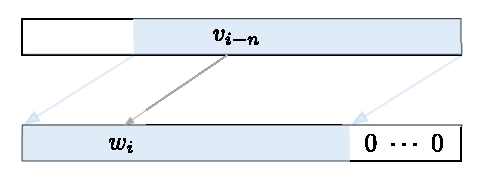
\includegraphics{figs/lsl}} &
\scalebox{.8}{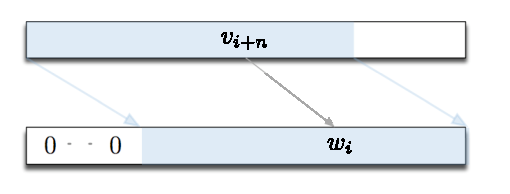
\includegraphics{figs/lsr}} \\
(a) Logical shift left: \holtxt{w = v << x}. & (b) Logical shift right:
\holtxt{w = v >>> x}. \\[12pt]
\scalebox{.8}{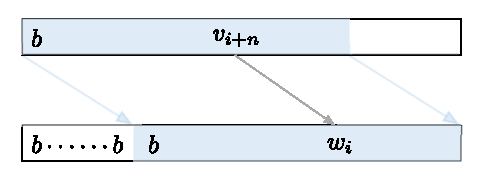
\includegraphics{figs/asr}} &
\hspace{-5mm}\scalebox{.8}{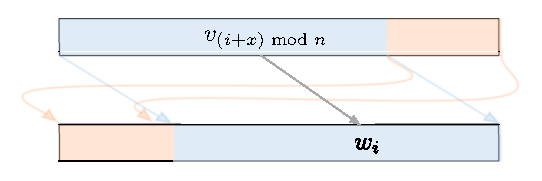
\includegraphics{figs/ror}} \\
(c) Arithmetic shift right: \holtxt{w = v >> x}. & (d) Rotate right: \holtxt{w
= v \#>> x}. \\[12pt]
\multicolumn{2}{c}{\scalebox{.8}{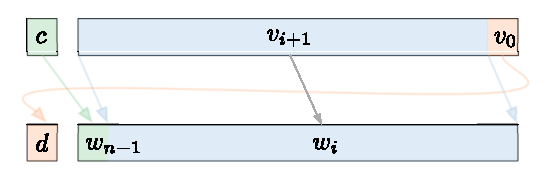
\includegraphics{figs/rrx}}} \\
\multicolumn{2}{c}{(e) Rotate right extended by 1 place: \holtxt{(d,w) =
word\_rrx (c,v)}.}
\end{tabular}
\caption{Shift operations.}
\label{fig:shifts}
\end{center}
\end{figure}

\paragraph{Aritmetica e ordinamenti}

Le operazioni aritmetiche sono: addizione, sottrazione, meno unario (coplemento a 
due), logaritmo (base-2), moltiplicazione, modulo e divisione (con e senza 
segno).
Queste operazioni sono definite rispetto ai numeri naturali. Per esempio, 
l'addizione parola � definita da:
\begin{hol}
\begin{verbatim}
|- !v w. v + w = n2w (w2n v + w2n w)
\end{verbatim}
\end{hol}
Il \holtxt{+} sul lato sinistro � un'addizione parola e quello sul lato destro � 
l'addizione sui numeri naturali.

Sono forniti tutti gli ordinamenti parola standard, con le versioni con e senza 
segno di $<$, $\leq$, $>$ e $\geq$. Le versioni senza segno hanno un suffisso 
con un pi�; per esempio, \holtxt{<+} � il ``minore di'' senza segno.

\paragraph{Costanti}

La teoria word definisce anche alcune costanti parola:
\begin{center}\small
\begin{tabular}{lll}
\multicolumn{1}{l}{Costante} & \multicolumn{1}{l}{Valore}  &
\multicolumn{1}{l}{Binario} \\
\noalign{\smallskip}
\hline
\noalign{\smallskip}
\holtxt{word\_T} or \holtxt{UINT\_MAXw} & $2^l - 1$ & $11\cdots 11$ \\
\holtxt{word\_L} or \holtxt{INT\_MINw} & $2^{l - 1}$ & $10\cdots 00$ \\
\holtxt{word\_H} or \holtxt{INT\_MAXw} & $2^{l - 1} - 1$ & $01\cdots 11$
\end{tabular}
\end{center}

\paragraph{Elenco di operazioni su vettori di bit}

Un elenco di operazioni � fornito nella tabella di sotto.
{
\setlength{\tabcolsep}{4pt}
\begin{center}
\tablefirsthead{%
\hline
\multicolumn{1}{|c}{Operazione\rule{0pt}{14pt}} &
\multicolumn{1}{c}{Simbolo} &
Type &
\multicolumn{1}{c|}{Descrizione} \\[4pt]
\hline}
\tablehead{%
\hline
\multicolumn{4}{|l|}{\small\sl continua dalla pagina precedente}\\
\hline
\multicolumn{1}{|c}{Operazione\rule{0pt}{14pt}} &
\multicolumn{1}{c}{Simbolo} &
Type &
\multicolumn{1}{c|}{Descrizione} \\[4pt]
\hline}
\tabletail{%
\hline
\multicolumn{4}{|r|}{\small\sl continua sulla pagina successiva}\\
\hline}
\tablelasttail{\hline}
\small
\begin{supertabular}{|l|c|l|l|}
\holtxt{n2w} & & \num\rarr\worda & Map from a natural number \\
\holtxt{w2n} & & \worda\rarr\num & Map to a natural number \\
\holtxt{w2w} & & \worda\rarr\wordb & Map word-to-word (unsigned) \\
\holtxt{sw2sw} & & \worda\rarr\wordb & Map word-to-word (signed) \\
\holtxt{w2l} & & \num\rarr\worda\rarr\num~\ty{list} & Map word to digit list \\
\holtxt{l2w} & & \num\rarr\num~\ty{list}\rarr\worda & Map digit list to word \\
\holtxt{w2s} & & \num\rarr(\num\rarr\ty{char})\rarr\worda\rarr\ty{string} & Map word to string \\
\holtxt{s2w} & & \num\rarr(\ty{char}\rarr\num)\rarr\ty{string}\rarr\worda & Map string to word \\
\holtxt{word\_len} & & \worda\rarr\num & The word length \\
\holtxt{word\_lsb} & & \worda\rarr\bool & The least significant bit \\
\holtxt{word\_msb} & & \worda\rarr\bool & The most significant bit \\
\holtxt{word\_bit} & & \num\rarr\worda\rarr\bool & Test bit position \\
\holtxt{word\_bits} & \holtxt{--} & \num\rarr\num\rarr\worda\rarr\worda & Select a bit field \\
\holtxt{word\_signed\_bits} & \holtxt{---} & \num\rarr\num\rarr\worda\rarr\worda & Sign-extend selected bit field \\
\holtxt{word\_slice} & \holtxt{''} & \num\rarr\num\rarr\worda\rarr\worda &  Set bits outside field to zero \\
\holtxt{word\_extract} & \holtxt{><} & \num\rarr\num\rarr\worda\rarr\wordb & Extract (cast) a bit field \\
\holtxt{word\_reverse} & & \worda\rarr\worda & Reverse the bit order \\
\holtxt{bit\_field\_insert} & & {\setlength{\tabcolsep}{0pt}\begin{tabular}[t]{ll}\num\rarr\num\rarr\worda\rarr\\\wordb\rarr\wordb\end{tabular}} & Insert a bit field \\
\holtxt{word\_modify} & & {\setlength{\tabcolsep}{0pt}\begin{tabular}[t]{ll}(\num\rarr\bool\rarr\bool)\rarr\\\worda\rarr\worda\end{tabular}} & Apply a function to each bit \\
\holtxt{word\_join} & & \worda\rarr\wordb\rarr\fcp{\bool}{$\alpha+\beta$} & Join words \\
\holtxt{word\_concat} & \holtxt{@@} & \worda\rarr\wordb\rarr\wordc & Concatenate words \\
\holtxt{concat\_word\_list} & & \worda~\ty{list}\rarr\wordb & Concatenate list of words \\
\holtxt{word\_replicate} & & \num\rarr\worda\rarr\wordb & Replicate word \\
\holtxt{word\_or} & \holtxt{||} & \worda\rarr\worda\rarr\worda & Bitwise disjunction \\
\holtxt{word\_xor} & \holtxt{??} & \worda\rarr\worda\rarr\worda & Bitwise exclusive-or \\
\holtxt{word\_and} & \holtxt{\&\&} & \worda\rarr\worda\rarr\worda & Bitwise conjunction \\
\holtxt{word\_nor} & \holtxt{\~{}||} & \worda\rarr\worda\rarr\worda & Bitwise NOR \\
\holtxt{word\_xnor} & \holtxt{\~{}??} & \worda\rarr\worda\rarr\worda & Bitwise XNOR \\
\holtxt{word\_nand} & \holtxt{\~{}\&\&} & \worda\rarr\worda\rarr\worda & Bitwise NAND \\
\holtxt{word\_reduce} & & {\setlength{\tabcolsep}{0pt}\begin{tabular}[t]{ll}(\bool\rarr\bool\rarr\bool)\rarr\\\worda\rarr\fcp{\bool}{1}\end{tabular}} & Word reduction \\
\holtxt{reduce\_or} & & \worda\rarr\fcp{\bool}{1} & Disjunction reduction \\
\holtxt{reduce\_xor} & & \worda\rarr\fcp{\bool}{1} & Exclusive-or reduction \\
\holtxt{reduce\_and} & & \worda\rarr\fcp{\bool}{1} & Conjunction reduction \\
\holtxt{reduce\_nor} & & \worda\rarr\fcp{\bool}{1} & NOR reduction \\
\holtxt{reduce\_xnor} & & \worda\rarr\fcp{\bool}{1} & XNOR reduction \\
\holtxt{reduce\_nand} & & \worda\rarr\fcp{\bool}{1} & NAND reduction \\
\holtxt{word\_{}1comp} & \holtxt{\~} & \worda\rarr\worda & One's complement \\
\holtxt{word\_{}2comp} & \holtxt{-} & \worda\rarr\worda & Two's complement \\
\holtxt{word\_add} & \holtxt{+} & \worda\rarr\worda\rarr\worda & Addition \\
\holtxt{word\_sub} & \holtxt{-} & \worda\rarr\worda\rarr\worda & Subtraction \\
\holtxt{word\_mul} & \holtxt{*} & \worda\rarr\worda\rarr\worda & Multiplication \\
\holtxt{word\_div} & \holtxt{//} & \worda\rarr\worda\rarr\worda & Division (unsigned) \\
\holtxt{word\_sdiv} & \holtxt{/} & \worda\rarr\worda\rarr\worda & Division (signed) \\
\holtxt{word\_mod} & & \worda\rarr\worda\rarr\worda & Modulus \\
\holtxt{word\_log2} & & \worda\rarr\worda & Logarithm base-2 \\
\holtxt{word\_lsl} & \holtxt{<<} & \worda\rarr\num\rarr\worda & Logical shift left \\
\holtxt{word\_lsr} & \holtxt{>>>} & \worda\rarr\num\rarr\worda & Logical shift right \\
\holtxt{word\_asr} & \holtxt{>>} & \worda\rarr\num\rarr\worda & Arithmetic shift right \\
\holtxt{word\_ror} & \holtxt{\#>>} & \worda\rarr\num\rarr\worda & Rotate right \\
\holtxt{word\_rol} & \holtxt{\#<<} & \worda\rarr\num\rarr\worda & Rotate left \\
\holtxt{word\_rrx} & & \bool\#\worda\rarr\bool\#\worda & Rotate right extended by 1 place \\
\holtxt{word\_lt} & \holtxt{<} & \worda\rarr\worda\rarr\bool & Signed ``less than'' \\
\holtxt{word\_le} & \holtxt{<=} & \worda\rarr\worda\rarr\bool & Signed ``less than or equal'' \\
\holtxt{word\_gt} & \holtxt{>} & \worda\rarr\worda\rarr\bool & Signed ``greater than'' \\
\holtxt{word\_ge} & \holtxt{>=} & \worda\rarr\worda\rarr\bool & Signed ``greater than or equal'' \\
\holtxt{word\_lo} & \holtxt{<+} & \worda\rarr\worda\rarr\bool & Unsigned ``less than''  \\
\holtxt{word\_ls} & \holtxt{<=+} & \worda\rarr\worda\rarr\bool & Unsigned ``less than or equal'' \\
\holtxt{word\_hi} & \holtxt{>+} & \worda\rarr\worda\rarr\bool & Unsigned ``greater than'' \\
\holtxt{word\_hs} & \holtxt{>=+} & \worda\rarr\worda\rarr\bool & Unsigned ``greater than or equal'' \\
\end{supertabular}
\end{center}}

\index{vettori di bit, la teoria HOL dei@vettori di bit, la teoria \HOL{} dei|)}
} % matches bracket at beginning of n-bit section, where some n-bit
  % specific macros are defined

\section{Sequenze}

\HOL{} fornisce teorie per vari generi di sequenze: liste finite, liste lazy, 
percorsi, e stringhe finite.

\subsection{Liste}\label{avra_list}
\index{list, l'operatore di tipo ... nella logica HOL@\ml{list}, l'operatore di tipo ... nella logica \HOL{}}
\index{tipi, nella logica HOL@tipi, nella logica \HOL{}!strumenti per la costruzione di}
\index{liste, la teoria HOL dei@liste, la teoria \HOL{} dei|(}
\index{ liste, la teoria HOL dei@\ml{[} $\cdots$ \ml{;} $\cdots$ \ml{]} (liste, la teoria \HOL{} dei)|(}

Le liste \HOL{} sono sequenze finite definite induttivamente dove ogni 
elemento in una lista ha lo stesso tipo. La teoria \ml{list} introduce 
l'operatore di tipo unario $\alpha \; \konst{list}$ per mezzo di una definizione di tipo 
ed � definita una collezione standard di funzioni di elaborazioni di 
liste. I costruttori primitivi {\small\verb+NIL+} e {\small\verb+CONS+}
%
\begin{hol}
\index{NIL, la costante HOL@\holtxt{NIL}, la costante \HOL{}}
\index{CONS, la costante HOL@\holtxt{CONS}, la costante \HOL{}}
\begin{verbatim}
   NIL  : 'a list
   CONS : 'a -> 'a list -> 'a list
\end{verbatim}
\end{hol}
%
sono usati per costruire liste e sono state definite dal tipo rappresentante per 
le liste. Il parser \HOL{}
%
\index{parsing, della logica HOL@parsing, della logica \HOL{}!delle espressioni lista}
%
� stato modificato in modo speciale per eseguire il parsing dell'espressione \holtxt{[]} in 
\holtxt{NIL}, per eseguire il parsing dell'espressione \holtxt{h::t} in \holtxt{CONS
  h t}, e il parsing dell'espressione \holtxt{[$t_1$;$t_2$;\dots;$t_n$]}
in \holtxt{CONS $t_1$ (CONS $t_2$ $\cdots$ (CONS $t_n$ NIL)
  $\cdots$)}. Il printer di \HOL{}
%
\index{printing, nella logica HOL@printing, nella logica \HOL{}!delle espressioni lista}
%
inverte queste trasformazioni.

\index{teoremi sulle liste, nella logica HOL@teoremi sulle liste, nella logica \HOL{}}
Sulla base della caratterizzazione induttiva del tipo, i seguenti 
teoremi fondamentali sulle liste sono dimostrati e archiviati nella teoria 
\ml{list}.

\begin{hol}
\index{list_Axiom@\ml{list\_Axiom}}
\index{assiomi!non-primitivi, della logica HOL@non-primitivi, della logica \HOL{}!per le liste}
\index{teoremi d'induzione, nella logica HOL@teoremi d'induzione, nella logica \HOL{}!per le liste}
\index{teorema caratterizzante!per le liste}
\begin{verbatim}
   list_Axiom
     |- !x f. ?fn. (fn [] = x) /\ (!h t. fn (h::t) = f(fn t)h t)
   list_INDUCT
     |- !P. P [] /\ (!t. P t ==> (!h. P(h::t))) ==> (!l. P l)
   list_CASES
     |- !l. (l = []) \/ (?t h. l = h::t)
   CONS_11
     |- !h t h' t'. (h::t = h'::t') = (h = h') /\ (t = t')
   NOT_NIL_CONS
     |- !h t. ~([] = h::t)
   NOT_CONS_NIL
     |- !h t. ~(h::t = [])
\end{verbatim}
\end{hol}

Il teorema \ml{list\_Axiom} mostrato di sopra � analogo al teorema di 
ricorsione primitiva 
%
\index{teorema di ricorsione primitiva!per le liste}
%
sui numeri naturali discusso di sopra nella Sezione~\ref{num-prim-rec}. 
Esso afferma la validit� delle definizioni ricorsive primitive sulle liste, 
e pu� essere usato per giustificare qualsiasi di tali definizioni. La funzione \ML{} 
\ml{new\_recursive\_definition} usa questo teorema per fare 
%
\index{teorema di ricorsione primitiva!uso automatizzato del, nel sistema HOL@uso automatizzato del, nel sistema \HOL{}|)}
%
dimostrazioni di esistenza delle funzioni ricorsive primitive sulle liste e 
quindi fare specifiche di costanti per introdurre costanti che denotano 
tali funzioni.

Il teorema d'induzione per le liste, \ml{list\_INDUCT}, fornisce lo strumento 
di dimostrazione principale usato per ragionare su operazioni che manipolano liste. Il 
teorema \ml{list\_CASES} � usato per eseguire l'analisi dei casi riguardo al fatto che una 
lista sia vuota o meno.

Il teorema {\small\verb+CONS_11+}  mostra che {\small\verb+CONS+} � iniettiva; 
i teoremi {\small\verb+NOT_NIL_CONS+} e {\small\verb+NOT_CONS_NIL+} mostrano che 
{\small\verb+NIL+} e {\small\verb+CONS+} sono distinte, cio�, 
non possono dare origine alla stessa struttura. Insieme, questi tre teoremi 
sono usati per il ragionamento equazionale circa le liste.

Il predicato \ml{NULL} e i selettori 
%
\index{selettori, nella logica HOL@selettori, nella logica \HOL{}!per le liste}
%
\ml{HD} e \ml{TL} sono definiti nella teoria \theoryimp{list} da
%
\begin{hol}
\index{NULL, la costante HOL@\ml{NULL}, la costante \HOL{}}
\index{HD, la costante HOL@\ml{HD}, la costante \HOL{}}
\index{TL, la costante HOL@\ml{TL}, la costante \HOL{}}
\begin{verbatim}
   NULL |- NULL [] /\ (!h t. ~NULL(h::t))
   HD   |- !h t. HD(h::t) = h
   TL   |- !h t. TL(h::t) = t
\end{verbatim}
\end{hol}

\noindent Nella teoria \ml{list} sono definite anche le seguenti funzioni.
%
%
\paragraph{Espressioni case}
\index{espressioni case!sulle liste}

Le espressioni composte \HOL{} che ramificano sulla base del fatto che un termine sia 
un lista vuota o non vuota hanno la sintassi di superficie (grossomodo presa in prestito 
dall'ML)
\begin{hol}
\begin{verbatim}
   case e1
    of [] => e2
     | (h::t) => e3
\end{verbatim}
\end{hol}
%
Una tale espressione � tradotta in
$\holtxt{list\_CASE}\ e_1\ e_2\ (\lambda h\; t.\ e_3)$ dove la costante 
\holtxt{list\_CASE} � definita come segue:
\begin{hol}
\begin{verbatim}
   list_case_def
     |- (!v f. list_CASE [] v f = v) /\
        (!v f a0 a1. list_CASE (a0::a1) v f = f a0 a1)
\end{verbatim}
\end{hol}

\paragraph{Appartenenza a una lista}
\index{MEM, la costante HOL@\ml{MEM}, la costante \HOL{}}

L'appartenenza a una lista, \ml{MEM}, � definita come segue:
%
\begin{hol}
\begin{verbatim}
   MEM |- (!x. MEM x [] = F) /\
          (!x h t. MEM x (h::t) = (x = h) \/ MEM x t)
\end{verbatim}
\end{hol}

\paragraph {Concatenazione di liste}
\index{APPEND, la costante HOL@\ml{APPEND}, la costante \HOL{}}
\index{concatenazione di liste!nella logica HOL@nella logica \HOL{}}
\index{FLAT, la costante HOL@\ml{FLAT}, la costante \HOL{}}

La concatenazione binaria di liste ({\small\verb+APPEND+}) pu� anche essere denotata 
dall'operatore infisso {\small\verb|++|}; cos� l'espressione 
{\small\verb|L1 ++ L2|} � tradotta in {\small\verb+APPEND L1 L2+}. 
La concatenazione di una lista di liste in una lista � ottenuta da 
{\small\verb+FLAT+}.
%
\begin{hol}
\begin{verbatim}
   APPEND
     |- (!l. APPEND [] l = l) /\
        (!l1 l2 h. APPEND (h::l1) l2 = h::APPEND l1 l2)
   FLAT
     |- (FLAT [] = []) /\ (!h t. FLAT(h::t) = h ++ FLAT t)
\end{verbatim}
\end{hol}

\paragraph {Numeri e liste}
\index{LENGTH, la costante HOL@\ml{LENGTH}, la costante \HOL{}}
\index{EL, la costante HOL@\ml{EL}, la costante \HOL{}}
\index{list_size, la costante HOL@\ml{list\_size}, la costante \HOL{}}

La lunghezza (\holtxt{LENGTH}) e la dimensione (\holtxt{list\_size}) di una lista 
sono nozioni correlate. La dimensione di una lista tiene conto della dimensione di 
ciascun elemento della lista (data dal parametro 
$f:\alpha\to\konst{num}$), mentre la lunghezza della lista ignora la 
dimensione di ciascun elemento della lista. La definizione alternativa della lunghezza 
(\holtxt{LEN}) � tail-recursive. Si possono inoltre usare numeri come indici 
nelle liste, estraendo l'elemento alla posizione specificata.
%
\begin{hol}
\begin{verbatim}
   LENGTH
     |- (LENGTH [] = 0) /\ (!h t. LENGTH (h::t) = SUC(LENGTH t))
   LEN_DEF
     |- (!n. LEN [] n = n) /\ !h t n. LEN (h::t) n = LEN t (n + 1)
   list_size_def
     |- (!f. list_size f [] = 0) /\
        !f a0 a1. list_size f (a0::a1) = 1 + (f a0 + list_size f a1))
   EL
     |- (!l. EL 0 l = HD l) /\ (!l n. EL (SUC n) l = EL n (TL l))
\end{verbatim}
\end{hol}

\noindent
Si noti che l'estrazione dell'elemento $n$-esimo (\holtxt{EL}) di una lista 
inizia la sua indicizzazione da 0. Se la lunghezza della lista $\ell$ � minore 
o uguale a $n$, il risultato di \holtxt{EL~$n$~$\ell$~} non � 
specificato.

\paragraph {Funzioni di mapping sulle liste}
\index{MAP, la costante HOL@\ml{MAP}, la costante \HOL{}}
\index{MAP2, la costante HOL@\ml{MAP2}, la costante \HOL{}}
\index{funzioni di mapping, nella logica HOL@funzioni di mapping, nella logica \HOL{}!per liste}

Ci sono delle funzioni per mappare una funzione $f : \alpha \to \beta$ su 
una singola lista (\holtxt{MAP}) o una funzione $f : \alpha \to \beta
\to \gamma$ sopra due liste (\holtxt{MAP2}).
\begin{hol}
\begin{verbatim}
   MAP
     |- (!f. MAP f [] = []) /\
        (!f h t. MAP f (h::t) = f h::MAP f t)
   MAP2
     |- (!f. MAP2 f [] [] = []) /\
        !f h1 t1 h2 t2. MAP2 f (h1::t1) (h2::t2) = f h1 h2::MAP2 f t1 t2
\end{verbatim}
\end{hol}
Il comportamento di \holtxt{MAP2} nel caso in cui le siano date liste di 
lunghezza diversa � indeterminato.

\paragraph {Predicati su liste}
\index{FILTER, la costante HOL@\ml{FILTER}, la costante \HOL{}}
\index{EVERY, la costante HOL@\ml{EVERY}, la costante \HOL{}}
\index{ALL_DISTINCT, la costante HOL@\ml{ALL\_DISTINCT}, la costante \HOL{}}
\index{EXISTS, la costante HOL (sulle liste)@\ml{EXISTS}, la costante \HOL{}
  (sulle liste)}

I predicati possono essere applicati a liste in un senso universale (il predicato 
deve valere per ogni elemento nella lista) o in un senso esistenziale (il 
predicato deve valere per qualche elemento nella lista). Questa funzionalit� 
� supportata da \holtxt{EVERY} e \holtxt{EXISTS}, rispettivamente. L'eliminazione 
di tutti gli elementi in una lista che non soddisfano il predicato dato 
� eseguita da \holtxt{FILTER}.
\begin{hol}
\begin{verbatim}
   EVERY_DEF
     |- (!P. EVERY P [] = T) /\
        (!P h t. EVERY P (h::t) = P h /\ EVERY P t)
   EXISTS_DEF
     |- (!P. EXISTS P [] = F) /\
        (!P h t. EXISTS P (h::t) = P h \/ EXISTS P t)
   FILTER
     |- (!P. FILTER P [] = []) /\
        (!P h t. FILTER P (h::t) = if P h then h::FILTER P t else FILTER P t)
   ALL_DISTINCT
     |- (ALL_DISTINCT [] = T) /\
        (!h t. ALL_DISTINCT (h::t) = ~MEM h t /\ ALL_DISTINCT t)
\end{verbatim}
\end{hol}
Il predicato \holtxt{ALL\_DISTINCT} vale su una lista solo nel caso in cui 
nessun elemento nella lista � uguale ad uno qualsiasi degli altri.

\paragraph {Folding}
\index{FOLDL, la costante HOL@\ml{FOLDL}, la costante \HOL{}}
\index{FOLDR, la costante HOL@\ml{FOLDR}, la costante \HOL{}}

L'applicare una funzione binaria $f : \alpha\to\beta\to\beta$ in modo accoppiato 
attraverso una lista e accumulando il risultato � conosciuto come 
\emph{folding}. A volte, � necessario eseguire questa operazione 
da sinistra a destra (\holtxt{FOLDL}), e altre volte � richieste la 
direzione da destra a sinistra (\holtxt{FOLDR}).
\begin{hol}
\begin{verbatim}
   FOLDL
     |- (!f e. FOLDL f e [] = e) /\
        (!f e x l. FOLDL f e (x::l) = FOLDL f (f e x) l)
   FOLDR
     |- (!f e. FOLDR f e [] = e) /\
        (!f e x l. FOLDR f e (x::l) = f x (FOLDR f e l))
\end{verbatim}
\end{hol}

\paragraph {Capovolgimento di liste}

Il capovolgimento di una lista (\holtxt{REVERSE}) e la sua controparte 
tail recursive \holtxt{REV} sono definite in \theoryimp{list}.
\begin{hol}
\begin{verbatim}
   REVERSE_DEF
     |- (REVERSE [] = []) /\
        (!h t. REVERSE (h::t) = REVERSE t ++ [h])
   REV_DEF
     |- (!acc. REV [] acc = acc) /\
        (!h t acc. REV (h::t) acc = REV t (h::acc))
\end{verbatim}
\end{hol}

\paragraph {Conversione a insiemi}

Le liste possono essere convertite in insiemi (\ml{LIST\_TO\_SET}) attraverso l'applicazione 
parziale di of \holtxt{MEM}. La definizione in qualche modo concisa � usata per 
derivare il teorema \ml{IN\_LIST\_TO\_SET}.
%
\begin{hol}
\begin{verbatim}
  LIST_TO_SET
    |- LIST_TO_SET = combin$C MEM
  IN_LIST_TO_SET
    |- x IN LIST_TO_SET l = MEM x l
	$
\end{verbatim}
\end{hol}
%
Ulteriore supporto per tradurre tra differenti generi di 
collezioni si pu� trovare nella teoria \theoryimp{container}.

\paragraph {Coppie e liste}

Due liste di uguale lunghezza possono essere accoppiate componente per componente attraverso 
l'operazione {\small\verb+ZIP+}. Il risultato non � specificato 
quando le liste non sono della stessa lunghezza. L'operazione inversa, 
{\small\verb+UNZIP+}, traduce una lista di coppie in una coppia di 
liste.
\begin{hol}
\begin{verbatim}
  ZIP
    |- (ZIP ([],[]) = []) /\
       (!x1 l1 x2 l2. ZIP (x1::l1,x2::l2) = (x1,x2)::ZIP (l1,l2))
  UNZIP_THM
    |- (UNZIP [] = ([],[])) /\
       (UNZIP ((x,y)::t) = let (L1,L2) = UNZIP t in (x::L1,y::L2))
\end{verbatim}
\end{hol}

\paragraph {Accesso alternativo}
\index{LAST, la costante HOL@\ml{LAST}, la costante \HOL{}}
\index{FRONT, la costante HOL@\ml{FRONT}, la costante \HOL{}}
%
Le liste sono trattate essenzialmente in modo simile a uno stack. Tuttavia, a 
volte � conveniente accedere all'ultimo elemento 
(\holtxt{LAST}) di una lista non vuota in modo diretto. L'ultimo elemento 
di una lista non vuota � eliminato attraverso \holtxt{FRONT}.
\begin{hol}
\begin{verbatim}
  LAST_DEF
    |- !h t. LAST (h::t) = if t = [] then h else LAST t
  FRONT_DEF
    |- !h t. FRONT (h::t) = if t = [] then [] else h::FRONT t
  APPEND_FRONT_LAST
    |- !l. ~(l = []) ==> (FRONT l ++ [LAST l] = l)
\end{verbatim}
\end{hol}
%
Concatenare la parte frontale e l'ultimo elemento di una lista non vuota porta 
alla lista originale. Entrambi \holtxt{LAST} e \holtxt{FRONT} 
sono non specificate su liste vuote.


\paragraph {Controllo prefisso}

\index{isPREFIX, la costante HOL@\ml{isPREFIX}, la costante \HOL{}}
La relazione che cattura se una lista $\ell_1$ � un prefisso di $\ell_2$ 
({\holtxt{isPREFIX}) pu� essere definita per ricorsione. L'infisso 
\holtxt{<{}<=} pu� anche essere usato come una notazione per questo ordine parziale.
% use of {} above is just a trick to stop Emacs font-lock colouring
% this file disgustingly
%
\begin{hol}
\begin{verbatim}
   isPREFIX_THM
     |- ([] <<= l <=> T) /\
        (h::t <<= [] <=> F) /\
        (h1::t1 <<= h2::t2 <=> (h1 = h2) /\ t1 <<= t2)
\end{verbatim}
\end{hol}
Il teorema di sopra afferma che: la lista vuota � un prefisso di ogni altra 
lista (clausola 1); che nessuna lista non vuota � un prefisso della lista vuota 
(clausola 2); e che una lista non vuota � un prefisso di un'altra lista 
non vuota se i primi elementi delle liste sono gli stessi, e se la coda 
della prima � un prefisso della coda della seconda.

\vspace{1ex}
\noindent Per una lista completa dei teoremi disponibili in 
\theoryimp{list}, si veda \REFERENCE. Un ulteriore sviluppo della teoria 
delle liste si pu� trovare in \theoryimp{rich\_list}.


\subsubsection{Permutazioni e ordinamento di liste}
\index{permutazioni (di liste), la teoria HOL delle@permutazioni (di liste), la teoria \HOL{} delle}
\index{ordinamento, la teoria HOL del@ordinamento, la teoria \HOL{} del}

La teoria \theoryimp{sorting} definisce la nozione per cui due liste sono 
permutazioni l'una dell'altra, poi definisce una nozione generale di ordinamento, 
quindi mostra che Quicksort � una funzione di ordinamento.

\paragraph{Permutazione di liste}

Due liste sono in permutazione se hanno esattamente gli stessi membri, 
e ogni membro ha lo stesso numero di occorrenze in entrambe le liste. Una 
definizione (\holtxt{PERM}) che cattura questa relazione � la 
seguente:
%
\begin{hol}
\begin{verbatim}
   PERM_DEF
     |- !L1 L2. PERM L1 L2 = !x. FILTER ($= x) L1 = FILTER ($= x) L2
   PERM_IND =
     |- !P.
          P [] [] /\
          (!x l1 l2. P l1 l2 ==> P (x::l1) (x::l2)) /\
          (!x y l1 l2. P l1 l2 ==> P (x::y::l1) (y::x::l2)) /\
          (!l1 l2 l3. P l1 l2 /\ P l2 l3 ==> P l1 l3)
         ==>
         !l1 l2. PERM l1 l2 ==> P l1 l2
\end{verbatim}
\end{hol}
%
Un teorema di induzione derivato (\holtxt{PERM\_IND}) � molto 
utile nelle dimostrazioni circa le permutazioni.

\paragraph{Ordinamento}

Una lista � $R$-ordinata se $R$ vale a coppie attraverso la lista. Questa 
nozione (\holtxt{SORTED}) � catturata da una definizione ricorsiva. Quindi 
una funzione di tipo
%
\begin{hol}
\begin{verbatim}
   ('a -> 'a -> bool) -> 'a list -> 'a list
\end{verbatim}
\end{hol}
%
� una funzione di ordinamento (\holtxt{SORTS}) rispetto a $R$ se 
emette una permutazione del suo input, e il risultato � $R$-ordinato.
%
\begin{hol}
\begin{verbatim}
   SORTED_DEF
     |- (SORTED R [] = T) /\
        (SORTED R [x] = T) /\
        (SORTED R (x::y::rst) = R x y /\ SORTED R (y::rst))
   SORTS_DEF
     |- !f R. SORTS f R = !l. PERM l (f R l) /\ SORTED R (f R l)
\end{verbatim}
\end{hol}
%
Quicksort � definito nell'usuale stile di programmazione funzionale, ed 
� di fatto una funzione di ordinamento, purch� $R$ sia una relazione 
transitiva e totale.
%
\begin{hol}
\begin{verbatim}
   QSORT_DEF =
     |- (QSORT ord [] = []) /\
        (QSORT ord (h::t) =
           let (l1,l2) = PARTITION (\y. ord y h) t
           in
             QSORT ord l1 ++ [h] ++ QSORT ord l2)
   QSORT_SORTS
     |- !R. transitive R /\ total R ==> SORTS QSORT R
\end{verbatim}
\end{hol}



\index{liste, la teoria HOL delle@liste, la teoria \HOL{} delle|)}
\index{ liste, la teoria HOL delle@\ml{[} $\cdots$ \ml{;} $\cdots$ \ml{]} (liste, la teoria \HOL{} delle)|)}

\subsection{Sequenze potenzialmente infinite (\theoryimp{llist})}

\index{liste lazy, la teoria HOL delle@liste ``lazy'', la teoria \HOL{} delle|(}

La teoria \theoryimp{llist} contiene la definizione di un tipo di 
sequenze potenzialmente infinite. Questo tipo � analogo alle ``liste 
lazy'' di linguaggi di programmazione come l'Haskell, da qui il nome 
della teoria. La teoria \theoryimp{llist} ha un numero di costanti che 
sono analoghe alle costanti nella teoria delle liste 
finite. Le versioni \theoryimp{llist} di queste costanti hanno gli 
stessi nomi, ma con una `L\/' maiuscola anteposta. Cos�, alcune delle costanti 
core in questa teoria sono:
\begin{hol}
\begin{verbatim}
   LNIL  : 'a llist
   LCONS : 'a -> 'a llist -> 'a llist
   LHD   : 'a llist -> 'a option
   LTL   : 'a llist -> 'a llist option
\end{verbatim}
\end{hol}

Le costanti \ml{LHD} e \ml{LTL} restituiscono \ml{NONE} quando applicate alla 
sequenza vuota, \ml{LNIL}. Questo uso di un tipo opzione � un altro 
modo di modellare la parzialit� essenziale di queste costanti. (Nella 
teoria delle liste, le analoghe funzioni \ml{HD} e \ml{TL} hanno 
semplicemente dei valori non specificati quando applicate alle liste vuote.)

Il tipo \ml{llist} non � induttivo, e non c'� alcun teorema di 
ricorsione primitiva che supporti la definizione di funzioni che hanno 
domini di tipo \ml{llist}. Piuttosto, \ml{llist} � un tipo coinduttivo, 
e ha un assioma che giustifica la definizione di funzioni 
(co-)ricorsive che mappano \emph{al} tipo \ml{llist}:
\begin{hol}
\begin{verbatim}
   llist_Axiom
      |- !f : 'a -> ('a # 'b) option.
           ?g : 'a -> 'b llist.
             (!x. LHD (g x) = OPTION_MAP SND (f x)) /\
             (!x. LTL (g x) = OPTION_MAP (g o FST) (f x))
\end{verbatim}
\end{hol}
\noindent Una forma equivalente a quella di sopra
\begin{hol}
\begin{verbatim}
   llist_Axiom_1
      |- !f. ?g.
           !x. g x =
               case f x
                of NONE => LNIL
                 | SOME (x',y) => LCONS y (g x')
\end{verbatim}
\end{hol}

Altre costanti, nella teoria \theoryimp{llist} includono \ml{LMAP}, \ml{LFINITE},
\ml{LNTH}, \ml{LTAKE}, \ml{LDROP}, e \ml{LFILTER}. I loro tipi sono
%
\index{mapping di funzioni, nella logica HOL@mapping di funzioni, nella logia \HOL{}!per sequenze potenzialmente infinite}
\begin{hol}
\begin{verbatim}
   LMAP    : ('a -> 'b) -> 'a llist -> 'b llist
   LFINITE : 'a llist -> bool
   LNTH    : num -> 'a llist -> 'a option
   LTAKE   : num -> 'a llist -> 'a list option
   LDROP   : num -> 'a llist -> 'a llist option
   LFILTER : ('a -> bool) -> 'a llist -> 'a llist
\end{verbatim}
\end{hol}
Esse sono caratterizzate dai seguenti teoremi
\begin{hol}
\begin{verbatim}
   LMAP
      |- (LMAP f LNIL = LNIL) /\
         (LMAP f (LCONS h t) = LCONS (f h) (LMAP f t))
   LFINITE_THM
      |- (LFINITE LNIL = T) /\
         (LFINITE (LCONS h t) = LFINITE t)
   LNTH_THM
      |- (!n. LNTH n LNIL = NONE) /\
         (!h t. LNTH 0 (LCONS h t) = SOME h) /\
         (!n h t. LNTH (SUC n) (LCONS h t) = LNTH n t)
   LTAKE_THM
      |- (LTAKE 0 l = SOME []) /\
         (LTAKE (SUC n) LNIL = NONE) /\
         (LTAKE (SUC n) (LCONS h t) = OPTION_MAP (CONS h) (LTAKE n t)
   LDROP_THM
      |- (LDROP 0 ll = SOME ll) /\
         (LDROP (SUC n) ll = NONE) /\
         (LDROP (SUC n) (LCONS h t) = LDROP n t)
   LFILTER_THM
      |- (LFILTER P LNIL = LNIL) /\
         (LFILTER P (LCONS h t) = if P h then LCONS h (LFILTER P t)
                                         else LFILTER P t)
\end{verbatim}
\end{hol}

\paragraph{Concatenazione}

Due liste lazy possono essere concatenate per mezzo di \ml{LAPPEND}. Se la prima lista 
lazy � infinita, gli elementi della seconda sono inaccessibili nel 
risultato. Una lista lazy di liste lazy pu� essere appiattita per mezzo 
di \ml{LFLATTEN}.
\begin{hol}\begin{verbatim}
   LAPPEND
      |- (!x. LAPPEND LNIL x = x) /\
         (!h t x. LAPPEND (LCONS h t) x = LCONS h (LAPPEND t x))
   LFLATTEN_THM
      |- (LFLATTEN LNIL = LNIL) /\
         (!tl. LFLATTEN (LCONS LNIL t) = LFLATTEN t) /\
         (!h t tl. LFLATTEN (LCONS (LCONS h t) tl) =
                      LCONS h (LFLATTEN (LCONS t tl)))
\end{verbatim}\end{hol}

\paragraph{Liste e liste lazy}

Il mapping da liste a liste lazy e vice versa si ottiene 
per mezzo di \ml{fromList} and \ml{toList}:
\begin{hol}\begin{verbatim}
   fromList
      |- (fromList [] = LNIL) /\
         (!h t. fromList (h::t) = LCONS h (fromList t))
   toList_THM
      |- (toList LNIL = SOME []) /\
         (!h t. toList (LCONS h t) = OPTION_MAP (CONS h) (toList t))
\end{verbatim}\end{hol}

\paragraph{Principi di dimostrazione}

In fine, ci sono due principi di dimostrazione molto importanti per dimostrare 
che due valori \ml{llist} sono uguali. Il primo afferma che due 
sequenze sono uguali se restituiscono gli stessi prefissi di lunghezza $n$ per 
tutti i valori possibili di $n$:
\begin{hol}
\begin{verbatim}
   LTAKE_EQ |- (ll1 = ll2) = (!n. LTAKE n ll1 = LTAKE n ll2)
\end{verbatim}
\end{hol}
Questo teorema � usato successivamente per derivare il principio 
di bi-simulazione:
\begin{hol}
\begin{verbatim}
   LLIST_BISIMULATION
            |- (ll1 = ll2) =
               ?R. R ll1 ll2 /\
                   !ll3 ll4. R ll3 ll4 ==>
                             (ll3 = LNIL) /\ (ll4 = LNIL) \/
                             (LHD ll3 = LHD ll4) /\
                             R (THE (LTL ll3)) (THE (LTL ll4))
\end{verbatim}
\end{hol}
Il principio di bi-simulazione afferma che due valori \ml{llist} $l_1$ 
e $l_2$ sono uguali se (e solo se) � possibile trovare una 
relazione $R$ tale che
\begin{itemize}
\item $R$ collega i due valori, cio�, $R\;l_1\;l_2$; and
\item se $R$ vale di due valori qualsiasi $l_3$ e $l_4$, allora o 
  \begin{itemize}
  \item entrambi $l_3$ e $l_4$ sono vuoti; o
  \item gli elementi testa di $l_3$ e $l_4$ sono gli stessi, e le 
		code di quei due valori sono di nuovo collegati da $R$
  \end{itemize}
\end{itemize}
Naturalmente, un $R$ possibile � l'eguaglianza stessa, ma la forza 
di questo teorema � che possono essere usate anche altre relazioni 
pi� convenienti.
\index{liste lazy, la teoria HOL delle@liste ``lazy'', la teoria \HOL{} delle|)}

\subsection{Percorsi etichettati (\theoryimp{path})}

La teoria \theoryimp{path}
%
\index{percorsi etichettati, la teoria HOL dei@percorsi etichettati, la teoria \HOL{} dei|(}
\index{sequenze di riduzione, la teoria HOL delle@sequenze di riduzione, la teoria \HOL{} delle|(}
\index{percorsi (sequenze di riduzione), la teoria HOL delle@percorsi (sequenze di riduzione), la teoria \HOL{} delle|(}
%
definisce un operatore di tipo binario $(\alpha,\beta)\ml{path}$, che 
sta per percorsi potenzialmente infiniti della seguente forma
\[
  \alpha_1 \stackrel{\beta_1}{\longrightarrow}
  \alpha_2 \stackrel{\beta_2}{\longrightarrow}
  \alpha_3 \stackrel{\beta_3}{\longrightarrow} \cdots
  \alpha_n \stackrel{\beta_n}{\longrightarrow}
  \alpha_{n+1} \stackrel{\beta_{n+1}}{\longrightarrow}  \cdots
  \]
Il tipo \ml{path} � cos� un modello appropriato per sequenze 
di riduzione, dove il parametro $\alpha$ corrisponde a ``stati'', e 
il parametro $\beta$ corrisponde alle etichette sulle frecce.

Il modello di $(\alpha,\beta)\ml{path}$ � $\alpha \times
((\alpha\times\beta)\ml{llist})$. Il tipo dei percorsi ha due 
costruttori:
\begin{hol}
\begin{verbatim}
   stopped_at : 'a -> ('a,'b) path
   pcons      : 'a -> 'b -> ('a,'b) path -> ('a,'b) path
\end{verbatim}
\end{hol}
Il costruttore \holtxt{stopped\_at} restituisce un percorso che contiene solo uno 
stato, e nessuna transizione. (Cos�, la sequenza di riduzione ha 
questo stato ``fermato'' [``stopped at'' ndt].) Il costruttore \ml{pcons} prende uno stato, 
un'etichetta, e un percorso, e restituisce un percorso che � ora intestato 
dall'argomento stato, e che si sposta da quello stato attraverso l'argomento etichetta 
al percorso. Graficamente, $\ml{pcons}\;x\;l\;p$ � uguale a
\[
x \stackrel{l}{\longrightarrow}
\underbrace{p_1 \stackrel{l_1}{\longrightarrow} p_2
  \stackrel{l_2}{\longrightarrow} \cdots\quad}_p
\]
Altre costanti definite nella teoria \theoryimp{path} includono
%
\index{funzioni di mapping, nella logica HOL@funzioni di mapping, nella logica \HOL{}!per percorsi etichettati}
%
\begin{hol}
\begin{verbatim}
   finite  : ('a,'b) path -> bool
   first   : ('a,'b) path -> 'a
   labels  : ('a,'b) path -> 'b llist
   last    : ('a,'b) path -> 'a
   length  : ('a,'b) path -> num option
   okpath  : ('a -> 'b -> 'a -> bool) -> ('a,'b) path -> bool
   pconcat : ('a,'b) path -> 'b -> ('a,'b) path -> ('a,'b) path
   pmap    : ('a -> 'c) -> ('b -> 'd) -> ('a,'b)path -> ('c,'d)path
\end{verbatim}
\end{hol}

La funzione \ml{first} restituisce il primo elemento di un percorso.
C'� sempre un tale elemento, e le equazioni di definizione sono
\begin{hol}
\begin{verbatim}
   first_thm  |- (first (stopped_at x) = x) /\
                 (first (pcons x l p) = x)
\end{verbatim}
\end{hol}

Dall'altro lato, la funzione \ml{last} non ha sempre un 
valore ben-specificato, bench� abbia ancora delle eleganti equazioni 
di caratterizzazione.
\begin{hol}
\begin{verbatim}
   last_thm   |- (last (stopped_at x) = x) /\
                 (last (pcons x l p) = last p)
\end{verbatim}
\end{hol}

Il teorema per \ml{finite} ha un aspetto simile, ma ha un valore 
definito (\ml{F}, o \emph{false}) su percorsi infiniti, mentre il 
valore di \ml{last} su tali percorsi non � specificato:
\begin{hol}
\begin{verbatim}
   finite_thm |- (finite (stopped_at x) = T) /\
                 (finite (pcons x l p) = finite p)
\end{verbatim}
\end{hol}

La funzione \ml{pconcat} concatena due percorsi, collegandoli 
con un'etichetta fornita. Se il primo percorso � infinito, allora il risultato 
� uguale a quello del primo percorso. Le equazioni di definizioni � 
\begin{hol}
\begin{verbatim}
   pconcat_thm |- (pconcat (stopped_at x) lab p2 = pcons x lab p2) /\
                  (pconcat (pcons x r p) lab p2 =
                       pcons x r (pconcat p lab p2)
\end{verbatim}
\end{hol}
%
Queste equazioni sono vere persino quando il primo argomento a 
\ml{pconcat} � un percorso infinito.

Il predicato \ml{okpath} testa se un percorso � o meno una transizione 
valida data una relazione di transizione ternaria. Il suo teorema 
di caratterizzazione �
\begin{hol}
\begin{verbatim}
  okpath_thm |-
     (okpath R (stopped_at x)) /\
     (okpath R (pcons x r p) = R x r (first p) /\ okpath R p)
\end{verbatim}
\end{hol}
%
C'� anche un principio d'induzione che semplifica il ragionamento circa 
$R$-percorsi finiti:
%
\begin{hol}
\begin{verbatim}
   finite_okpath_ind |-
       (!x. P (stopped_at x)) /\
       (!x r p. okpath R p /\ finite p /\ R x r (first p) /\ P p ==>
                P (pcons x r p)) ==>
       !p. okpath R p /\ finite p ==> P p
\end{verbatim}
\end{hol}

Si pu� mostrare che un insieme \holtxt{P} di percorsi sono tutti $R$-percorsi con il 
principio di co-induzione:
\begin{hol}
\begin{verbatim}
   okpath_co_ind |-
      !P.
         (!x r p. P (pcons x r p) ==> R x r (first p) /\ P p) ==>
         !p. P p ==> okpath R p
\end{verbatim}
\end{hol}
\index{percorsi etichettati, la teoria HOL dei@percorsi etichettati, la teoria \HOL{} dei|)}
\index{sequenze di riduzione, la teoria HOL delle@sequenze di riduzione, la teoria \HOL{} delle|)}
\index{percorsi (sequenze di riduzione),la teoria HOL dei@percorsi (sequenze di riduzione), la teoria \HOL{} dei|)}


\subsection{Le stringhe di caratteri (\theoryimp{string})}
\index{stringhe, la teoria HOL delle@stringhe, la teoria \HOL{} delle|(}

La teoria \theoryimp{string} definisce un tipo di caratteri e un tipo 
di stringhe finite costruite da quei caratteri, insieme con un'utile suite di 
definizioni per operare su stringhe.

\paragraph {Caratteri}
\index{caratteri, la teoria HOL dei@caratteri, la teoria \HOL{} dei}

Il tipo \holtxt{char} � rappresentato dai numeri minori di 256. Sono 
definite due costanti: {\small\verb+CHR +}$: \konst{num}\to\konst{char}$ e
{\small\verb+ORD +}$: \konst{char}\to\konst{num}$. Valgono i seguenti 
teoremi:
\begin{hol}
\begin{verbatim}
  CHR_ORD  |- !a. CHR (ORD a) = a
  ORD_CHR  |- !r. r < 256 = (ORD (CHR r) = r)
\end{verbatim}
\end{hol}

\index{letterali carattere}
I letterali carattere possono essere inseriti usando la sintassi \ML{}, con un carattere 
hash immediatamente seguito da un letterale stringa di lunghezza uno.
Cos�:
\setcounter{sessioncount}{0}
\begin{session}
\begin{verbatim}
- val t = ``f #"c" #"\n"``;
<<HOL message: inventing new type variable names: 'a>>
> val t = ``f #"c" #"\n"`` : term

- dest_term ``#"\t"``;
> val it = COMB(``CHR``, ``9``) : lambda
\end{verbatim}
\end{session}



\paragraph {Stringhe}

Il tipo \holtxt{string} � un alias per il tipo \holtxt{char list}. 
Tutte le funzioni e i predicati sulle liste sono cos� disponibili per l'uso 
sulle stringhe. Alcune di queste costanti sono sottoposte a overload cos� che sono 
stampate (e possono essere elaborate dal parsing) con nomi che sono pi� appropriate per 
il particolare caso delle liste di caratteri.

Per esempio, \holtxt{NIL} e \holtxt{CONS} su liste hanno 
i nomi alternativi \holtxt{EMPTYSTRING} e \holtxt{STRING} 
rispettivamente:
%
\begin{hol}
\index{EMPTYSTRING, la costante HOL@\holtxt{EMPTYSTRING}, la costante \HOL{}}
\index{STRING, la costante HOL@\holtxt{STRING}, la costante \HOL{}}
\begin{verbatim}
   EMPTYSTRING : string
   STRING      : char -> string -> string
\end{verbatim}
\end{hol}
\index{letterali stringa}
Il parser \HOL{} mappa la sintassi \holtxt{""} a \holtxt{EMPTYSTRING}, 
e il printer \HOL{} inverte questo. Il parser espande i letterali 
stringa della forma \holtxt{"$c_1 c_2 \ldots c_n$"} al termine 
composto
\[
\holtxt{STRING} \;c_1\; (\holtxt{STRING}\;c_2\,\ldots\,
 (\holtxt{STRING} \;c_{n-1} \; (\holtxt{STRING}\;
c_n \; \holtxt{EMPTYSTRING})) \,\ldots\, )
\]
Naturalmente, si potrebbe anche scrivere
\begin{session}
\begin{verbatim}
- ``[#"a"; #"b"]``;
> val it = ``"ab"`` : term
\end{verbatim}
\end{session}

I letterali stringa possono essere costruiti usando le varie speciali sequenze 
di escape che sono usate in \ML{}. Per esempio, \ml{\bs{}n} per il 
carattere di nuova linea, e un backslash seguite da tre cifre decimali 
per caratteri del numero dato.
\begin{session}
\begin{verbatim}
- val t = ``"foo bar\n\001"``;
> val t = ``"foo bar\n\^A"`` : term
\end{verbatim}
\end{session}
Si noti che se si vuole usare la sintassi di controllo caratteri con il 
caret che il pretty-printer ha scelto di usare per stampare la stringa 
data, e questo accade all'interno di una quotation, allora il caret dovr� 
essere duplicato. (Si veda la Sezione~\ref{sec:quotation-antiquotation}.)

C'� anche una funzione de-costruttore {\small\verb+DEST_STRING+} per 
le stringhe che restituisce un tipo opzione.
\begin{hol}
\begin{verbatim}
   DEST_STRING
     |- (DEST_STRING "" = NONE) /\
        (DEST_STRING (STRING c rst) = SOME(c,rst))
\end{verbatim}
\end{hol}


\paragraph{Espressioni case}
\index{espressioni case!su stringhe}

Le espressioni \HOL{} composte che ramificano sulla base del fatto che 
un termine sia una stringa vuota o non vuota possono essere scritte con la 
sintassi di superficie
\begin{hol}
\begin{verbatim}
   case s
    of "" => e1
     | STRING c rst => e2
\end{verbatim}
\end{hol}

Una tale espressione � di fatto un'espressione case sulla lista sottostante, e cos� la costante sottostante � quella per le liste.

\paragraph {Lunghezza e concatenazione}

Una funzione standard \holtxt{LENGTH} pu� essere scritta \holtxt{STRLEN} 
quando applicata a una stringa, e \holtxt{APPEND} pu� essere scritta come 
\holtxt{STRCAT}. Ci sono anche teoremi che caratterizzano queste 
costanti in \ml{stringTheory}, bench� esse siano semplicemente istanziazioni 
dei risultati da \ml{listTheory}:
\begin{hol}
\begin{verbatim}
   STRLEN_THM
     |- (STRLEN "" = 0) /\
        (STRLEN (STRING c s) = 1 + STRLEN s)

   STRCAT_EQNS =
     |- (STRCAT "" s = s) /\
        (STRCAT s "" = s) /\
        (STRCAT (STRING c s1) s2 = STRING c (STRCAT s1 s2))
\end{verbatim}
\end{hol}


\index{stringhe, la teoria HOL delle@stringhe, la teoria \HOL{} delle|)}

\section{Collezioni}

In \HOL{} sono disponibili alcune nozioni differenti di collezione di elementi: 
insiemi, multi-insiemi, relazioni, e mappe finite.

\subsection{Insiemi (\theoryimp{pred\_set})}
\label{sec:theory-of-sets}
\index{insiemi, la teoria HOL dei@insiemi, la teoria \HOL{} dei}

Un esteso sviluppo della teoria degli insiemi � disponibile nella teoria 
\theoryimp{pred\_set}. Gli insiemi sono rappresentati da funzione del tipo 
$\alpha \to \konst{bool}$, cio�, essi sono le cosiddette funzioni 
caratteristiche.
%
\index{funzioni caratteristiche!come base della teoria \HOL{} degli insiemi}
%
Si pu� usare l'abbreviazione di tipo $\alpha\; \konst{set}$ 
al posto di $\alpha \to \konst{bool}$. Gli insiemi possono essere finiti o 
infiniti. Tutti gli elementi in un insieme devono avere lo stesso tipo.

L'\emph{appartenenza a un insieme} � la nozione base sui cui � basata la teoria degli insiemi 
formalizzata. In \HOL, l'appartenenza � rappresentata da una costante 
infissa \holtxt{IN}, definita per convenienza nella teoria 
\theoryimp{bool}.
\begin{hol}
\begin{verbatim}
   IN_DEF   |- IN = \x f. f x
\end{verbatim}
\end{hol}
L'operatore \holtxt{IN} � semplicemente un modo di applicare la 
funzione caratteristica a un elemento, come mostra la seguente conseguenza 
banale della definizione:
\begin{hol}
\begin{verbatim}
   SPECIFICATION   |- !P x. x IN P = P x
\end{verbatim}
\end{hol}
Due insiemi sono uguali se hanno gli stessi elementi.
\begin{hol}
\begin{verbatim}
   EXTENSION   |- !s t. (s = t) = (!x. (x IN s) = (x IN t))
\end{verbatim}
\end{hol}

\paragraph{Insiemi vuoti e universali}
\index{insieme universale}
L'insieme vuoto � la funzione caratteristica che � costantemente falsa. La costante \holtxt{EMPTY} denota l'insieme vuoto; essa pu� essere scritta come \holtxt{\{\}} and \holtxt{$\emptyset$} (U+2205).
L'insieme universale, \holtxt{UNIV}, su un tipo � la funzione caratteristica che � sempre vera per elementi di quel tipo.
\begin{hol}
\begin{verbatim}
   EMPTY_DEF   |- {} = (\x. F)
   UNIV_DEF    |- UNIV = (\x. T)
\end{verbatim}
\end{hol}
In aggiunta a \holtxt{UNIV} (magari con un'annotazione di tipo \holtxt{:'a~set}), si pu� anche  scrivere \holtxt{univ(:'a)} per rappresentare l'insieme universale sul tipo \holtxt{:'a}.
La sintassi Unicode \holtxt{$\mathbb{U}$(:'a)} significa la stessa cosa. 
Il simbolo Unicode per $\mathbb{U}$ � U+1D54C, e potrebbe non esistere in molti set di font.

Una di queste forme sar� usata per stampare \holtxt{UNIV} di default. 
La traccia utente (si veda la Sezione~\ref{sec:traces}) \ml{"Univ~pretty-printing"} pu� essere impostata a zero per cancellare questo comportamento. 
Inoltre, la traccia \ml{"Unicode Univ printing"} pu� essere usata per smettere di usare la sintassi U+1D54C, persino se � attiva la traccia Unicode.

I simboli \holtxt{univ} e \holtxt{$\mathbb{U}$} sono prefissi di priorit� alta (si veda la Sezione~\ref{sec:parseprint:fixities}), e pattern sottoposti a overload (si veda la Sezione~\ref{sec:parser:syntactic-patterns}) che mappano un valore dello tipo stesso alla costante corrispondente \holtxt{UNIV}.
Un effetto � che si pu� scrivere cose del tipo
\begin{hol}
\begin{verbatim}
   FINITE univ(:'a)
\end{verbatim}
\end{hol}
senza il bisogno di parentesi intorno all'argomento di \holtxt{FINITE}.

\paragraph{Inserimento, unione, e intersezione}

L'inserimento ({\small\verb+INSERT+}, scritto infisso) di un elemento 
in un insieme � definito con una comprensione d'insieme. La comprensione d'insieme � 
discussa nella sottosezione successiva. Le definizioni usuali per l'unione insiemistica ({\small\verb+UNION+},
scritto infisso) e l'intersezione ({\small\verb+INTER+}, anch'esso infisso) 
sono date attraverso la comprensione d'insieme.
\begin{hol}
\begin{verbatim}
   INSERT_DEF  |- !x s. x INSERT s = {y | (y = x) \/ y IN s}
   UNION_DEF   |- !s t. s UNION t = {x | x IN s \/ x IN t}
   INTER_DEF   |- !s t. s INTER t = {x | x IN s /\ x IN t}
\end{verbatim}
\end{hol}
\holtxt{UNION} e \holtxt{INTER} sono operazioni 
binarie. Le operazioni di unione e intersezione indicizzata, cio�, 
$\bigcup_{i \in P}$ e $\bigcap_{i \in P}$ sono fornite dalle 
definizioni di \holtxt{BIGUNION} e \holtxt{BIGINTER}.
\begin{hol}
\begin{verbatim}
   BIGUNION    |- !P. BIGUNION P = {x | ?s. s IN P /\ x IN s}
   BIGINTER    |- !P. BIGINTER P = {x | !s. s IN P ==> x IN s}
\end{verbatim}
\end{hol}
Sia \holtxt{BIGUNION} che \holtxt{BIGINTER} riducono un insieme di insiemi a un 
insieme e cos� hanno il tipo 
$((\alpha\to\konst{bool})\to\konst{bool})\to (\alpha\to\konst{bool})$.

\paragraph{Sottoinsiemi}

L'inclusione di insiemi (\holtxt{SUBSET}, infisso), l'inclusione propria 
(\holtxt{PSUBSET}, infisso), e l'insieme potenza (\holtxt{POW}) sono definite come 
segue:
%
\begin{hol}
\begin{verbatim}
   SUBSET_DEF  |- !s t. s SUBSET t = !x. x IN s ==> x IN t
   PSUBSET_DEF |- !s t. s PSUBSET t = s SUBSET t /\ ~(s = t)
   POW_DEF     |- !set. POW set = {s | s SUBSET set}
\end{verbatim}
\end{hol}

\paragraph{Differenza di insiemi e complemento}

La differenza tra due insiemi (\holtxt{DIFF}, infisso) � definita da una 
comprensione di insieme. Sulla base di quella, la cancellazione di un singolo elemento 
(\holtxt{DELETE}, infisso) da un insieme � diretta. Dal momento che 
l'universo di un tipo � sempre disponibile attraverso \holtxt{UNIV}, si pu� prendere il 
complemento (\holtxt{COMPL}) di un insieme.
\begin{hol}
\begin{verbatim}
   DIFF_DEF    |- !s t. s DIFF t = {x | x IN s /\ ~(x IN t)}
   DELETE_DEF  |- !s x. s DELETE x = s DIFF {x}
   COMPL_DEF   |- !P. COMPL P = UNIV DIFF P
\end{verbatim}
\end{hol}

\paragraph{Funzioni su insiemi}
L'immagine di una funzione $f :\alpha \to \beta$ su 
un insieme (\holtxt{IMAGE}) � definito con una comprensione d'insieme.
\begin{hol}
\begin{verbatim}
   IMAGE_DEF   |- !f s. IMAGE f s = {f x | x IN s}
\end{verbatim}
\end{hol}
%
Iniezioni, suriezioni, e biezioni tra insiemi sono definite 
come segue:
%
\begin{hol}
\begin{verbatim}
   INJ_DEF
        |- !f s t.
             INJ f s t =
             (!x. x IN s ==> f x IN t) /\
             !x y. x IN s /\ y IN s ==> (f x = f y) ==> (x = y)
   SURJ_DEF
        |- !f s t.
             SURJ f s t =
             (!x. x IN s ==> f x IN t) /\
             !x. x IN t ==> ?y. y IN s /\ (f y = x)

   BIJ_DEF |- !f s t. BIJ f s t = INJ f s t /\ SURJ f s t
\end{verbatim}
\end{hol}

\paragraph{Insiemi finiti}
\index{finitezza!di insiemi}
Gli insiemi finiti (\holtxt{FINITE}) sono definiti induttivamente come quelli 
costruiti dall'insieme vuoto per mezzo di un numero finito di inserimenti.
%
\begin{hol}
\begin{verbatim}
   FINITE_DEF
     |- !s. FINITE s = !P. P {} /\ (!s. P s ==> !e. P (e INSERT s)) ==> P s
\end{verbatim}
\end{hol}
%
\noindent
Un insieme � infinito sse non � finito, e c'� un'abbreviazione nel sistema che esegue il parsing di \holtxt{\holquote{INFINITE~s}} in \holtxt{\holquote{\td{}FINITE~s}}.
Il pretty-printer inverte questa trasformazione.

\medskip\noindent
Gli insiemi finiti hanno un teorema d'induzione:
%
\index{teoremi d'induzione, nella logica HOL@teoremi d'induzione, nella logica \HOL{}!per insiemi finiti}
%
\begin{hol}
\begin{verbatim}
   FINITE_INDUCT
     |- !P. P {} /\
           (!s. FINITE s /\ P s ==> !e. ~(e IN s) ==> P (e INSERT s))
           ==>  !s. FINITE s ==> P s
\end{verbatim}
\end{hol}
%
Come menzionato, le operazioni su insiemi si applicano sia a insiemi finiti che 
infiniti. Tuttavia, alcune operazioni, come la cardinalit� 
(\holtxt{CARD}), sono definite soltanto per insiemi finiti. La 
cardinalit� di un insieme infinito non � specificata.
\index{cardinalit� d'insiemi (finiti)}
%
\begin{hol}
\begin{verbatim}
   CARD_DEF
     |- (CARD {} = 0) /\
        !s. FINITE s ==>
            !x. CARD (x INSERT s) = if x IN s then CARD s else SUC (CARD s)
\end{verbatim}
\end{hol}
%
Dal momento che gli insiemi finiti e infiniti sono gestiti in modo uniforme in 
\theoryimp{pred\_set}, le propriet� delle operazioni su insiemi finiti devono 
includere esplicitamente dei vincoli circa la finitezza. Per esempio il 
seguente teorema che collega la cardinalit� e i sottoinsiemi � vero solo per 
insiemi finiti.
%
\begin{hol}
\begin{verbatim}
   CARD_PSUBSET
     |- !s. FINITE s ==> !t. t PSUBSET s ==> CARD t < CARD s
\end{verbatim}
\end{hol}
%
In \theoryimp{pred\_set} � disponibile un'estesa suite di teoremi che trattano 
con la finitezza e la cardinalit�.

\paragraph{Prodotto incrociato}
Il prodotto di due insiemi ({\small\verb+CROSS+}, infisso) � definito 
con una comprensione d'insieme.
%
\begin{hol}
\begin{verbatim}
   CROSS_DEF   |- !P Q. P CROSS Q = {p | FST p IN P /\ SND p IN Q}
\end{verbatim}
\end{hol}
%
\noindent La cardinalit� e il prodotto incrociato sono collegati dal seguente teorema:
\begin{hol}
\begin{verbatim}
   CARD_CROSS
     |- !P Q. FINITE P /\ FINITE Q ==> (CARD (P CROSS Q) = CARD P * CARD Q)
\end{verbatim}
\end{hol}

\paragraph{Funzioni ricorsive su insiemi}

Le funzioni ricorsive su insiemi possono essere definite dalla ricorsione 
benfondata. Di solito, la totalit� di una tale funzione � stabilita 
misurando la cardinalit� dell'insieme (finito). Tuttavia, si pu� usare 
un altro teorema per giustificare un fold ({\small\verb+ITSET+}) per insiemi finiti.
Purch� una funzione $f:\alpha\to\beta\to\beta$ obbedisca a una condizione 
conosciuta come \emph{commutativa-a-sinistra}, cio�, $f\;x\;(f\;y\;z) =
f\;y\;(f\;x\;z)$, allora $f$ pu� essere applicata eseguendo il suo folding sull'insieme 
in un modo tail-ricorsivo.
\begin{hol}
\begin{verbatim}
   ITSET_EMPTY
     |- !f b. ITSET f {} b = b
   COMMUTING_ITSET_INSERT
     |- !f s. (!x y z. f x (f y z) = f y (f x z)) /\ FINITE s ==>
              !x b. ITSET f (x INSERT s) b = ITSET f (s DELETE x) (f x b)
\end{verbatim}
\end{hol}
E' disponibile anche una versione ricorsiva:
\begin{hol}
\begin{verbatim}
   COMMUTING_ITSET_RECURSES
     |- !f e s b.
          (!x y z. f x (f y z) = f y (f x z)) /\ FINITE s ==>
          (ITSET f (e INSERT s) b = f e (ITSET f (s DELETE e) b))
\end{verbatim}
\end{hol}
For the full derivation, see the sources of {\small\verb+pred_set+}.
The definition of {\small\verb+ITSET+} allows, for example, the
definition of summing the results of a function on a finite set of
elements, from which a recursive characterization and other useful
theorems are derived.

Per la completa derivazione, si vedano i sorgenti di {\small\verb+pred_set+}. 
La definizione di {\small\verb+ITSET+} permette, per esempio, la 
definizione della sommatoria dei risultati di una funzione su un insieme finito di 
elementi, da cui sono derivati una caratterizzazione ricorsiva e altri utili 
teoremi.
%
\begin{hol}
\begin{verbatim}
   SUM_IMAGE_DEF
     |- !f s. SIGMA f s = ITSET (\e acc. f e + acc) s 0
   SUM_IMAGE_THM
     |- !f. (SIGMA f {} = 0) /\
            !e s. FINITE s ==>
                  (SIGMA f (e INSERT s) = f e + SIGMA f (s DELETE e))
\end{verbatim}
\end{hol}

\paragraph{Altre definizioni e teoremi}

TCi sono molte altre definizioni in \theoryimp{pred\_set}, ma non sono 
usate cos� pesantemente come quelle presentate qui. Analogamente, la maggior parte dei teoremi 
in \theoryimp{pred\_set} collegano varie operazioni comuni sugli insiemi l'una 
con le altre, ma non esprimono al cun teorema profondo della teoria degli insiemi.

Comunque, un teorema degno di nota � il Lemma di Koenig, che afferma che 
ogni albero infinito finitamente ramificato ha un percorso infinito. Ci sono 
molti modi di formulare questo teorema, a seconda di come la nozione di 
albero � formalizzata. In \theoryimp{pred\_set}, la ramificazione finita � 
definita come un predicato su una relazione.
%
\begin{hol}
\begin{verbatim}
   finite_branching_def
     |- !R. finitely_branching R = !x. FINITE {y | R x y}
\end{verbatim}
\end{hol}
%
Da questo, la seguente versione del Lemma di Koenig � enunciata e 
dimostrata:
\begin{hol}
\begin{verbatim}
   KoenigsLemma
     |- finitely_branching R ==>
          !x. ~FINITE {y | RTC R x y} ==>
              ?f. (f 0 = x) /\ !n. R (f n) (f (SUC n))
\end{verbatim}
\end{hol}


\subsubsection{Sintassi per gli insiemi}\index{notazione insiemistica}

Le notazioni insiemistiche special purpose 
{\small\verb%%} e
{\small\verb%{%}$t${\small\verb% | %}$p${\small\verb%}%} sono riconosciute 
dal parser e dal printer di \HOL{} quando la teoria \theoryimp{pred\_set} 
� caricata.

L'interpretazione normale di \lb$t_1 ;t_2 ; \ldots ; t_n$\rb{} � l'insieme finito 
che contiene solo $t_1,t_2,\ldots,
t_n$. Questo pu� essere modellato iniziando con l'insieme vuoto e 
eseguendo una sequenza di inserimenti. Per esempio, \holtxt{\lb{}1;2;3;4\rb{}} 
� parsato a

\begin{hol}
\begin{verbatim}
   1 INSERT (2 INSERT (3 INSERT (4 INSERT EMPTY)))
\end{verbatim}
\end{hol}

\paragraph {Comprensioni d'inseime}

L'interpretazione normale di
{\small\verb%{%}$t${\small\verb% | %}$p${\small\verb%}%} �
l'insieme di tutti i $t$ tali che $p$. In \HOL, tale sintassi � analizzata dal parser a:
%
\ml{GSPEC(\bs($x_1$,$\ldots$,$x_n$).($t$,$p$))}
%
\noindent dove $x_1, \ldots, x_n$ sono quelle variabili libere che 
occorrono sia in $t$ sia in $p$ se entrambi hanno almeno una variabile libera. Se 
$t$ o $p$ non hanno variabili libere, allora $x_1, \ldots, x_n$ sono considerate 
essere le variabili libere dell'altro termine. Se entrambi hanno variabili 
libere, ma non c'� sovrapposizione, allora risulta un errore. L'ordine 
in cui le variabili sono elencate nella struttura di variabili 
dell'astrazione accoppiata � una funzione nn specificata della struttura di $t$ 
(� approssimativamente da sinistra a destra). Per esempio,
%
\begin{hol}
\begin{verbatim}
   {p+q | p < q /\ q < r}
\end{verbatim}
\end{hol}
%
� analizzata dal parser a:
%
\begin{hol}
\begin{verbatim}
   GSPEC(\(p,q). ((p+q), (p < q /\ q < r)))
\end{verbatim}
\end{hol}
%
dove \ml{GSPEC} � caratterizzata da:
%
\begin{hol}
\begin{verbatim}
   GSPECIFICATION  |- !f v. (v IN GSPEC f) = (?x. (v,T) = f x)
\end{verbatim}
\end{hol}

Questa specifica in qualche modo criptica si pu� comprendere attraverso 
un esempio. La sintassi 
%
\begin{hol}
\begin{verbatim}
   a IN {p+q | p < q /\ q < r}
\end{verbatim}
\end{hol}
%
� mappata dal parser \HOL{} a
\begin{hol}
\begin{verbatim}
   a IN GSPEC(\(p,q). ((p+q), (p < q /\ q < r)))
\end{verbatim}
\end{hol}
%
che, per \ml{GSPECIFICATION}, � uguale a
\begin{hol}
\begin{verbatim}
   ?x. (a,T) = (\(p,q). ((p+q), (p < q /\ q < r))) x
\end{verbatim}
\end{hol}
%
La variabile quantificata esistenzialmente \verb+x+ ha un tipo coppia, 
cos� che pu� essere sostituita da una coppia \verb+(p,q)+ e 
si pu� eseguire una $\beta$-riduzione-accoppiata, portando a 
%
\begin{hol}
\begin{verbatim}
   ?(p,q). (a,T) = ((p+q), (p < q /\ q < r))
\end{verbatim}
\end{hol}
%
che � uguale al significato inteso della sintassi 
originale:
%
\begin{hol}
\begin{verbatim}
   ?(p,q). (a = p+q) /\ (p < q /\ q < r)
\end{verbatim}
\end{hol}

\paragraph{Comprensioni d'insieme non ambigue} C'� anche una sintassi 
della comprensione d'insieme non ambigua, che permetter all'utente di 
specificare quali variabili devono essere quantificate nell'astrazione 
cio� l'argomento di \holtxt{GSPEC}. Termini della forma 
\begin{hol}
\begin{verbatim}
   { t | vs | P }
\end{verbatim}
\end{hol}
generano insiemi che contengono valori della forma data da \holtxt{t}, dove 
le variabili menzionate in \holtxt{vs} devono soddisfare il vincolo 
\holtxt{P}. Per esempio, l'insieme 
\begin{hol}
\begin{verbatim}
   { x + y | x | x < y }
\end{verbatim}
\end{hol}
� l'insieme dei numeri da \holtxt{y} fino a ma non incluso 
\holtxt{2~*~y}. L'insieme pu� essere ``letto'' in modo computazionale: escludere tutte 
quelle \holtxt{x} che sono minori di \holtxt{y}, e ad ognuna di tali 
\holtxt{x} aggiungere \holtxt{y}, generando con ci� un insieme di numeri.

Nell'esempio di sopra, il termine \holtxt{GSPEC} sottostante sar�
\begin{hol}
\begin{verbatim}
   GSPEC (\x. (x + y, x < y))
\end{verbatim}
\end{hol}

Il componente \holtxt{vs} della notazione non ambigua deve essere una singola 
``struttura variabile'' che potrebbe apparire sotto un'astrazione possibilmente 
accoppiata come nella Sezione~\ref{HOL-varstruct}. In altre parole, questo
\begin{hol}
\begin{verbatim}
   { x + y | (x,y) | x < y }
\end{verbatim}
\end{hol}
va bene, ma questo 
\begin{hol}
\begin{verbatim}
   { x + y | x y | x < y }
\end{verbatim}
\end{hol}
sollever� un errore. (Inoltre, le parentesi pi� esterne intorno 
alle coppie nella posizione \holtxt{vs} si possono omettere.)

La notazione non ambigua � stampata dal pretty-printere ogni volta che 
l'insieme da stampare non pu� essere espressa con la notazione di default, o 
se la variabile di traccia con nome \ml{pp\_unambiguous\_comprehensions} 
� impostata a \ml{true}.


\subsection{Multi-insiemi (\theoryimp{bag})}\label{multiset}

I multinsiemi, anche conosciuti come \emph{bag}, sono simili agli insiemi, eccetto per il fatto che 
essi permettono occorrenze ripetute di un elemento. Mentre gli insiemi sono 
rappresentati da funzioni di tipo $\alpha\to\konst{bool}$, che segnalano 
la presenza, o l'assenza, di un elemento, i multinsiemi sono rappresentati 
da funzioni di tipo $\alpha\to\konst{num}$, che danno la 
molteplicit� di ciascun elemento nel multinsieme. I multinsiemi possono essere finiti 
o infiniti.

Le abbreviazioni di tipo $\alpha\;\konst{multiset}$ e
$\alpha\;\konst{bag}$ possono essere usate al posto di $\alpha\to\konst{num}$.

\paragraph {Multinsieme vuoto}

Il multinsieme vuoto non ha elementi. Cos�, la funzione che lo implementa 
restituisce $0$ per ogni input.
%
\begin{hol}
\begin{verbatim}
   EMPTY_BAG  |- EMPTY_BAG = K 0
\end{verbatim}
\end{hol}

\noindent La sintassi speciale {\verb+{||}+} pu� essere usata per rappresentare il multinsieme 
vuoto.

\paragraph {Appartenenza}

Much of the theory can be based on the notion of membership in a
bag. There are two notions: does an element occur at least $n$ times
in a bag ({\small\verb+BAG_INN+}); and does an element occur in a bag
at all ({\small\verb+BAG_IN+}).

La maggior parte della teoria si pu� basare sulla nozione di appartenenza a un 
multinsieme. Ci sono due nozioni: un elemento occorre al meno $n$ volte 
in una bag
%
\begin{hol}
\begin{verbatim}
   BAG_INN  |- BAG_INN e n b = (b e >= n)
   BAG_IN   |- BAG_IN e b = BAG_INN e 1 b
\end{verbatim}
\end{hol}
%
Due bag sono uguali se tutti gli elemento hanno lo stesso conteggio.
%
\begin{hol}
\begin{verbatim}
   BAG_EXTENSION
     |- !b1 b2. (b1 = b2) = (!n e. BAG_INN e n b1 = BAG_INN e n b2)
\end{verbatim}
\end{hol}

\paragraph{Sotto-multinsieme}

Una relazione sotto-bag (\holtxt{SUB\_BAG}) vale tra $b_1$ e
$b_2$ a condizione che ogni elemento in $b_1$ occorra almeno le stesse volte in 
$b_2$. La nozione di una sotto-bag propria (\holtxt{PSUB\_BAG}) � facilmente 
definita.
%
\begin{hol}
\begin{verbatim}
   SUB_BAG
     |- SUB_BAG b1 b2 = !x n. BAG_INN x n b1 ==> BAG_INN x n b2
   PSUB_BAG
     |- PSUB_BAG b1 b2 = SUB_BAG b1 b2 /\ ~(b1 = b2)
\end{verbatim}
\end{hol}

\paragraph{Inserimento}

L'inserimento di un elemento in una bag (\holtxt{BAG\_INSERT}) aggiorna il 
conteggio di quell'elemento e lascia gli altri inalterati.
%
\begin{hol}
\begin{verbatim}
   BAG_INSERT
     |- BAG_INSERT e b = (\x. if (x = e) then b e + 1 else b x)
\end{verbatim}
\end{hol}

Multinsiemi esplicitamente-dati sono supportati dalla sintassi 
{\small\verb%{|%}$t_1 ;t_2 ; \ldots ; t_n${\small\verb%|}%}, dove 
ci possono essere, naturalmente, ripetizioni. Questo � modellando iniziando con il multinsieme 
vuoto ed eseguendo una sequenza di inserimenti. Per esempio, 
\verb+{|1; 2; 3; 2; 1|}+ � analizzato dal parser a

\begin{hol}
\begin{verbatim}
   BAG_INSERT 1 (BAG_INSERT 2 (BAG_INSERT 3
                                 (BAG_INSERT 2 (BAG_INSERT 1 {||}))))
\end{verbatim}
\end{hol}


\paragraph{Unione and differenza}

Le operazioni di unione (\holtxt{BAG\_UNION}) e differenza (\holtxt{BAG\_DIFF}) 
su bag si riducono entrambe a un calcolo aritmetico sui loro 
elementi. L'eliminazione di un singolo elemento da un bag pu� essere espresso come il 
prendere la differenza tra il multinsieme con un multinsieme di un singolo elemento; 
tuttavia, c'� anche una presentazione relazionale 
(\holtxt{BAG\_DELETE}) che collega i suoi primi e ultimi argomenti solo 
se il primo contiene esattamente una occorrenza in pi� dell'argomento 
di mezzo rispetto all'ultimo. Questa non � la stessa cosa di usare 
\holtxt{BAG\_DIFF} per rimuovere una bag di un elemento perch� insiste sul fatto che 
l'elemento che viene rimosso appare effettivamente nella bag pi� grande.
%
\begin{hol}
\begin{verbatim}
   BAG_UNION
     |- BAG_UNION b c = \x. b x + c x
   BAG_DIFF
     |- BAG_DIFF b1 b2 = \x. b1 x - b2 x
   BAG_DELETE
     |- BAG_DELETE b0 e b = (b0 = BAG_INSERT e b)
\end{verbatim}
\end{hol}

\paragraph {Intersezione, merge, e filtro}

L'intersezione di due bag (\holtxt{BAG\_INTER}) prende il minimo 
puntuale. L'operazione duale, il merging (\holtxt{BAG\_MERGE}), prende il 
massimo puntuale. Una bag pu� essere `filtrata' da un insieme per restituire la bag 
dove tutti gli elementi che non sono nell'insieme sono stati rimossi.
%
\begin{hol}
\begin{verbatim}
   BAG_INTER
     |- BAG_INTER b1 b2 = (\x. if (b1 x < b2 x) then b1 x else b2 x)
   BAG_MERGE
     |- BAG_MERGE b1 b2 = (\x. if (b1 x < b2 x) then b2 x else b1 x)
   BAG_FILTER_DEF
     |- BAG_FILTER P b = (\e. if P e then b e else 0)
\end{verbatim}
\end{hol}

\paragraph {Insiemi e Multinsiemi}

Lo spostamento tra bag e insiemi si ottiene con le seguenti due 
definizioni
%
\begin{hol}
\begin{verbatim}
   SET_OF_BAG
     |- SET_OF_BAG b = \x. BAG_IN x b
   BAG_OF_SET
     |- BAG_OF_SET P = \x. if x IN P then 1 else 0
\end{verbatim}
\end{hol}

\paragraph {Immagine}

Prendere l'immagina di una funzione su un multinsieme per ottenere un nuovo multinsieme 
sembrerebbe essere semplicemente una questione di applicare la funzione a ciascun elemento 
del multinsieme. Tuttavia, c'� un problema se $f$ non � iniettiva 
e il multinsieme � infinito. Per esempio, si prenda il multinsieme 
che consiste di tutti i numeri naturali e si applichi $\lambda x.\; 1$ a 
ciascun elemento. Il multinsieme risultante conterrebbe un numero infinito di 
$1$. Per evitare questo sono richiesti alcuni vincoli: per esempio, 
stipulare che la funzione sia solo finitamente non-iniettiva, o che 
il multinsieme di input sia finito. Tali condizioni sarebbero onerose alla prova 
dei fatti; il compromesso � mappare la molteplicit� degli elementi 
problematici a $0$.
%
\begin{hol}
\begin{verbatim}
   BAG_IMAGE_DEF
     |- BAG_IMAGE f b =
          \e. let sb = BAG_FILTER (\e0. f e0 = e) b
              in
                if FINITE_BAG sb then BAG_CARD sb else 0
\end{verbatim}
\end{hol}


\paragraph {Multinsiemi finiti}
\index{finitezza!dei multinsiemi}
I multinsiemi finiti (\holtxt{FINITE\_BAG}) sono definiti in modo induttivo come 
quelli costruiti dalla bag vuota attraverso un numero finito di inserimenti.
%
\begin{hol}
\begin{verbatim}
   FINITE_BAG
     |- FINITE_BAG b =
          !P. P EMPTY_BAG /\
              (!b. P b ==> (!e. P (BAG_INSERT e b))) ==> P b
\end{verbatim}
\end{hol}
%
I multinsiemi finiti hanno un teorema d'induzione, e anche un teorema 
d'induzione completa.
%
\index{teoremi d'induzione, nella logica HOL@teoremi d'induzione, nella logica \HOL{}!per bag finite}
%
\begin{hol}
\begin{verbatim}
   FINITE_BAG_INDUCT
     |- !P. P {||} /\
            (!b. P b ==> (!e. P (BAG_INSERT e b)))
            ==> (!b. FINITE_BAG b ==> P b)

   STRONG_FINITE_BAG_INDUCT
     |- !P. P {||} /\
            (!b. FINITE_BAG b /\ P b ==> !e. P (BAG_INSERT e b))
            ==> (!b. FINITE_BAG b ==> P b)
\end{verbatim}
\end{hol}
%
La cardinalit� (\holtxt{BAG\_CARD}) di un multinsieme conta il 
numero totale di occorrenze. Essa � specificata solo per multinsiemi finiti.
%
\begin{hol}
\begin{verbatim}
   BAG_CARD_THM
     |- (BAG_CARD {||} = 0) /\
        (!b. FINITE_BAG b ==>
               !e. BAG_CARD (BAG_INSERT e b) = BAG_CARD b + 1)
\end{verbatim}
\end{hol}

\paragraph{Funzioni ricorsive su multinsiemi}

Le funzioni ricorsive su multinsiemi possono essere definite per ricorsione 
benfondata. Di solito, la totalit� di una tale funzione � stabilita 
misurando la cardinalit� del multinsieme (finito). Tuttavia, � fornito 
un fold (\holtxt{ITBAG}) per insiemi [multinsiemi? ndt] finiti. A condizione che una funzione 
$f:\alpha\to\beta\to\beta$ obbedisca a una condizione conosciuta come 
\emph{commutativit�-a-sinistra}, cio�, $f\;x\;(f\;y\;z) =
f\;y\;(f\;x\;z)$, allora $f$ pu� essere applicata eseguendone il folding sul 
multinsieme in una maniera tail-ricorsiva.
%
\begin{hol}
\begin{verbatim}
   ITBAG_EMPTY
     |- !f acc. ITSET f {||} acc = acc
   COMMUTING_ITBAG_INSERT
     |- !f b. (!x y z. f x (f y z) = f y (f x z)) /\ FINITE_BAG b ==>
              !x a. ITBAG f (BAG_INSERT x b) a = ITBAG f b (f x a)
\end{verbatim}
\end{hol}
%
E' disponibile anceh una versione ricorsiva:
\begin{hol}
\begin{verbatim}
   COMMUTING_ITBAG_RECURSES
     |- !f e b a. (!x y z. f x (f y z) = f y (f x z)) /\ FINITE_BAG b ==>
                  (ITBAG f (BAG_INSERT e b) a = f e (ITBAG f b a))
\end{verbatim}
\end{hol}

\subsection{Relazioni (\theoryimp{relation})}\label{relation}

Le relazioni matematiche possono essere rappresentate in \HOL{} dal tipo 
$\alpha \to\beta\to\konst{bool}$. (Nella maggior parte delle applicazioni, il tipo di una 
relazione � un'istanza di $\alpha \to\alpha\to\konst{bool}$, ma la 
generalit� extra non fa male.) La teoria \theoryimp{relation} 
fornisce definizioni delle propriet� e delle operazioni di base sulle relazioni, 
definisce vari generi di ordini e chiusure, definisce la benfondatezza 
e dimostra il teorema di ricorsione benfondata, e sviluppa alcuni 
risultati base usati nella Riscrittura dei Termini.

\paragraph {Propriet� base}

Le seguenti propriet� base delle relazioni sono definite.
%
\begin{hol}
\begin{verbatim}
   transitive_def
     |- transitive R = !x y z. R x y /\ R y z ==> R x z
   reflexive_def
     |- reflexive R = (!x. R x x)
   irreflexive_def
     |- irreflexive R = (!x. ~R x x)
   symmetric_def
     |- symmetric R = (!x y. R x y = R y x)
   antisymmetric_def
     |- antisymmetric R = (!x y. R x y /\ R y x ==> (x = y))
   equivalence_def
     |- equivalence R = reflexive R /\ symmetric R /\ transitive R
   trichotomous
     |- trichotomous R = !a b. R a b \/ R b a \/ (a = b)
   total_def
     |- total R = (!x y. R x y \/ R y x)
\end{verbatim}
\end{hol}

\paragraph{Operazioni base}

Le seguenti operazioni base sulle relazioni sono definite: la relazione 
vuota (\holtxt{EMPTY\_REL}), la composizione di relazione (\holtxt{O},
infisso), l'inversione (\holtxt{inv}), il dominio (\holtxt{RDOM}), e il rango 
(\holtxt{RRANGE}).
%
\begin{hol}
\begin{verbatim}
   EMPTY_REL_DEF
     |- !x y. EMPTY_REL x y = F
   O_DEF
     |- $O R1 R2 x z = ?y. R1 x y /\ R2 y z
   inv_DEF
     |- inv R x y = R y x
   RDOM_DEF
     |- RDOM R x = ?y. R x y
   RRANGE
     |- RRANGE R y = ?x. R x y
\end{verbatim}
\end{hol}

\noindent Le operazioni sugli insiemi riutilizzate per lavorare sulle relazioni includono il sottoinsieme 
(\holtxt{RSUBSET}, infisso), l'unione (\holtxt{RUNION}, infisso),
l'intersezione (\holtxt{RINTER}, infisso), il complemento (\holtxt{RCOMPL}),
e l'universo (\holtxt{RUNIV}).
%
\begin{hol}
\begin{verbatim}
   RSUBSET
     |- $RSUBSET R1 R2 = !x y. R1 x y ==> R2 x y
   RUNION
     |- $RUNION R1 R2 x y = R1 x y \/ R2 x y
   RINTER
     |- $RINTER R1 R2 x y = R1 x y /\ R2 x y
   RCOMPL
     |- RCOMPL R x y = ~R x y
   RUNIV
     |- RUNIV x y = T
\end{verbatim}
\end{hol}

\paragraph {Ordini}

In \theoryimp{relation} � fatta una serie di definizioni che catturano varie 
nozioni.
%
\begin{hol}
\begin{verbatim}
   PreOrder
     |- PreOrder R = reflexive R /\ transitive R
   Order
     |- Order Z = antisymmetric Z /\ transitive Z
   WeakOrder
     |- WeakOrder Z = reflexive Z /\ antisymmetric Z /\ transitive Z
   StrongOrder
     |- StrongOrder Z = irreflexive Z /\ antisymmetric Z /\ transitive Z
   LinearOrder
     |- LinearOrder R = Order R /\ trichotomous R
   WeakLinearOrder
     |- WeakLinearOrder R = WeakOrder R /\ trichotomous R
   StrongLinearOrder
     |- StrongLinearOrder R = StrongOrder R /\ trichotomous R
\end{verbatim}
\end{hol}

\paragraph {Chiusure}

La chiusura transitiva (\holtxt{TC}) di una relazione $R : \alpha
\to\alpha\to\konst{bool}$ � definita in modo induttivo, come la pi� piccola 
relazione che include $R$ ed � chiusa sotto la transitivit�. Analogamente, la 
chiusura riflessiva-transitiva (\holtxt{RTC}) � definita essere la pi� piccola 
relazione chiusa sotto la transitivit� e la riflessivit�.
%
\begin{hol}
\begin{verbatim}
   TC_DEF
     |- TC R a b =
          !P. (!x y. R x y ==> P x y) /\
              (!x y z. P x y /\ P y z ==> P x z) ==> P a b
   RTC_DEF
     |- RTC R a b =
          !P. (!x. P x x) /\
              (!x y z. R x y /\ P y z ==> P x z) ==> P a b
\end{verbatim}
\end{hol}

\noindent
Da queste definizioni, si possono recuperare le regole iniziali.
%
\begin{hol}
\begin{verbatim}
   TC_RULES
     |- !R. (!x y. R x y ==> TC R x y) /\
            (!x y z. TC R x y /\ TC R y z ==> TC R x z)
   RTC_RULES
     |- !R. (!x. RTC R x x) /\
            (!x y z. R x y /\ RTC R y z ==> RTC R x z)
   RTC_RULES_RIGHT1
     |- !R. (!x. RTC R x x) /\
            (!x y z. RTC R x y /\ R y z ==> RTC R x z)
\end{verbatim}
\end{hol}
%
Si noti che {\small\verb+RTC_RULES+}, in linea con la definizione 
di {\small\verb+RTC+}, estende un \verb+R+-passo da \verb+x+ a 
\verb+y+ con una sequenza di \verb+R+-passi da \verb+y+ a \verb+z+ 
per costruire \verb+RTC x z+. Il teorema 
{\small\verb+RTC_RULES_RIGHT1+} prima fa una serie di \verb+R+
passi e poi un singolo \verb+R+ passo per formare \verb+RTC x z+. Analoghi 
teoremi alternatici sono dimostrati per l'analisi dei casi e l'induzione.

Per esempio, {\small\verb+TC_CASES1+} e {\small\verb+TC_CASES2+} in ci� che 
segue de-compongono {\small\verb+RTC R x z+} o a 
{\small\verb+R x y+} seguito da {\small\verb+RTC R y z+}
({\small\verb+TC_CASES1+})
o a 
{\small\verb+RTC R x y+} seguito da {\small\verb+R y z+}
({\small\verb+TC_CASES2+}).

%
\begin{hol}
\begin{verbatim}
   TC_CASES1
     |- !R x z. TC R x z ==> R x z \/ ?y. R x y /\ TC R y z
   TC_CASES2
     |- !R x z. TC R x z ==> R x z \/ ?y. TC R x y /\ R y z

   RTC_CASES1
     |- !R x y. RTC R x y = (x = y) \/ ?u. R x u /\ RTC R u y
   RTC_CASES2
     |- !R x y. RTC R x y = (x = y) \/ ?u. RTC R x u /\ R u y
   RTC_CASES_RTC_TWICE
     |- !R x y. RTC R x y = ?u. RTC R x u /\ RTC R u y
\end{verbatim}
\end{hol}

Esattamente come i teoremi d'induzione di base per {\small\verb+TC+} e
{\small\verb+RTC+}, ci sono i cosiddetti teoremi d'induzione 
\emph{completa}, che hanno ipotesi d'induzione pi� forti.
%
\begin{hol}
\begin{verbatim}
   TC_INDUCT
     |- !R P. (!x y. R x y ==> P x y) /\
              (!x y z. P x y /\ P y z ==> P x z)
              ==> !u v. TC R u v ==> P u v
   RTC_INDUCT
     |- ! R P. (!x. P x x) /\
               (!x y z. R x y /\ P y z ==> P x z) ==>
               (!x y. RTC R x y ==> P x y)
   TC_STRONG_INDUCT
     |- !R P. (!x y. R x y ==> P x y) /\
              (!x y z. P x y /\ P y z /\ TC R x y /\ TC R y z ==> P x z) ==>
              (!u v. TC R u v ==> P u v)
   RTC_STRONG_INDUCT
     |- !R P. (!x. P x x) /\
              (!x y z. R x y /\ RTC R y z /\ P y z ==> P x z) ==>
              (!x y. RTC R x y ==> P x y)
\end{verbatim}
\end{hol}
Sono anche disponibili varianti di questi teoremi d'induzione che dividono 
la chiusura dalla sinistra o dalla destra, come per i teoremi di analisi dei casi.

\medskip

Le chiusure riflessiva~(\holtxt{RC}) e simmetrica~(\holtxt{SC}) sono 
facili da definire. La chiusura di equivalenza 
({\small\verb+EQC+}) � la chiusura simmetrica poi transitiva poi riflessiva 
di $R$.
%
\begin{hol}
\begin{verbatim}
   RC_DEF   |- RC R x y = (x = y) \/ R x y
   SC_DEF   |- SC R x y = R x y \/ R y x
   EQC_DEF  |- EQC R = RC (TC (SC R))
\end{verbatim}
\end{hol}

\paragraph {Relazioni benfondate}

Una relazione $R$ � benfondata ({\small\verb+WF+}) se ogni insieme non-vuoto 
ha un elemento $R$-minimo. La benfondatezza � usata per giustificare il 
principio d'induzione benfondata ({\small\verb+WF_INDUCTION_THM+}).
%
\begin{hol}
\begin{verbatim}
   WF_DEF
     |- !R. WF R = !B. (?w. B w) ==> ?min. B min /\ !b. R b min ==> ~B b
   WF_INDUCTION_THM
     |- !R WF R ==> !P. (!x. (!y. R y x ==> P y) ==> P x) ==> !x. P x
\end{verbatim}
\end{hol}

La \emph{parte benfondata} ({\small\verb+WFP+}) di una relazione pu� essere 
definita induttivamente, da essa possono essere derivate le sue regole, il teorema di analisi dei casi e 
i teoremi d'induzione.
%
\begin{hol}
\begin{verbatim}
   WFP_DEF
     |- WFP R a = !P. (!x. (!y. R y x ==> P y) ==> P x) ==> P a
   WFP_RULES
     |- !R x. (!y. R y x ==> WFP R y) ==> WFP R x
   WFP_CASES
     |- !R x. WFP R x = !y. R y x ==> WFP R y
   WFP_INDUCT
     |- !R P. (!x. (!y. R y x ==> P y) ==> P x)
              ==> !x. WFP R x ==> P x
   WFP_STRONG_INDUCT
     |- !R. (!x. WFP R x /\ (!y. R y x ==> P y) ==> P x)
            ==> !x. WFP R x ==> P x
\end{verbatim}
\end{hol}

La benfondatezza pu� essere usata anche per giustificare un teorema di ricorsione 
generale. Intuitivamente, una collezione di equazioni di ricorsione possono essere 
ammesse nella logica \HOL{} senza perdita di coerenza purch� 
ogni sequenza possibile di chiamate ricorsive sia finita. Le relazioni 
benfondate sono usate per catturare questa nozione: se c'� una relazione 
benfondata $R$ sul dominio della funzione desiderata tale che ogni 
sequenza di chiamate ricorsive � $R$-decrescente, allora le equazioni 
di ricorsione specificano un'unica funzione totale e le equazioni possono essere 
ammesse nella logica.

I teoremi di ricorsione {\small\verb+WFREC_COROLLARY+} e 
{\small\verb+WF_RECURSION_THM+} usano la nozione di una restrizione 
di funzione ({\small\verb+RESTRICT+}) al fine di forzare l'applicazione della funzione 
ricorsiva ad argomenti $R$-pi�-piccoli nelle chiamate ricorsive.
%
\begin{hol}
\begin{verbatim}
   RESTRICT_DEF
     |- !f R x. RESTRICT f R x = \y. if R y x then f y else ARB

   WFREC_COROLLARY
     |- !M R f. (f = WFREC R M) ==> WF R ==> !x. f x = M (RESTRICT f R x) x

   WF_RECURSION_THM
     |- !R. WF R ==> !M. ?!f. !x. f x = M (RESTRICT f R x) x
\end{verbatim}
\end{hol}

\noindent I teoremi {\small\verb+WF_INDUCTION_THM+} e
{\small\verb+WFREC_COROLLARY+} sono usati per automatizzare le definizioni 
ricorsive; si veda la Sezione \ref{TFL}. Sono anche definiti alcuni operatori 
di base per le relazioni benfondate, insieme con i teoremi che affermano 
che essi propagano la benfondatezza.

\begin{hol}
\begin{verbatim}
   inv_image_def  |- !R f. inv_image R f = \x y. R (f x) (f y)

   WF_inv_image   |- !R f. WF R ==> WF (inv_image R f)
   WF_SUBSET      |- !R P. WF R /\ (!x y. P x y ==> R x y) ==> WF P
   WF_TC          |- !R. WF R ==> WF (TC R)
   WF_Empty       |- WF EMPTY_REL
\end{verbatim}
\end{hol}

\paragraph {Riscrittura di termini}

Alcune definizioni di base prese dalla teoria della Riscrittura di Termini 
(la propriet� diamante (\verb+diamond+), la propriet� 
Church-Rosser ({\small\verb+CR+} e {\small\verb+WCR+}), e la Normalizzazione 
Forte ({\small\verb+SN+})) appaiono 
in \theoryimp{relation}.
%
\begin{hol}
\begin{verbatim}
   diamond_def
     |- diamond R = !x y z. R x y /\ R x z ==> ?u. R y u /\ R z u
   CR_def
     |- CR R = diamond (RTC R)
   WCR_def
     |- WCR R = !x y z. R x y /\ R x z ==> ?u. RTC R y u /\ RTC R z u
   SN_def
     |- SN R = WF (inv R)
\end{verbatim}
\end{hol}
%
Da queste, � dimostrato il Lemma di Newman.
%
\begin{hol}
\begin{verbatim}
   Newmans_lemma  |- !R. WCR R /\ SN R ==> CR R
\end{verbatim}
\end{hol}

\subsection{Mappe finite (\theoryimp{finite\_map})}\label{finite_map}

La teoria \theoryimp{finite\_map} formalizza un tipo 
$(\alpha,\beta)\,\holtxt{fmap}$ di funzioni finite. Queste teoricamente  
hanno il tipo $\alpha\to\beta$, ma in pi� hanno solo un numero finito di 
elementi nel loro dominio. Le mappe finite sono utili per formalizzare 
le sostituzioni e gli array. Il tipo rappresentate � $\alpha\to\beta +
\konst{one}$, dove solo un numero finito degli $\alpha$ mappano a un 
$\beta$ e il resto mappano a \verb+one+. la sintassi 
$\alpha\,\holtxt{|->}\,\beta$ � riconosciuta dal parser come 
un'alternativa a $(\alpha,\beta)\,\holtxt{fmap}$.

\paragraph {Nozioni base}

La mappa vuota (\holtxt{FEMPTY}), l'aggiornamento di una mappa 
(\holtxt{FUPDATE}), l'applicazione di una mappa a un argomento 
(\holtxt{FAPPLY}), e il dominio di una mappa (\holtxt{FDOM}) sono le 
nozioni principali nella teoria.
\begin{hol}
\begin{verbatim}
   FEMPTY  : 'a |-> 'b
   FUPDATE : ('a |-> 'b) -> 'a # 'b -> ('a |-> 'b)
   FAPPLY  : ('a |-> 'b) -> 'a -> 'b
   FDOM    : ('a |-> 'b) -> 'a set
\end{verbatim}
\end{hol}

Il parser e il printer \HOL{} tratteranno la sintassi \holtxt{f\,'\,x} come 
l'applicazione della mappa finita \verb+f+ to argument \verb+x+, cio�, come 
\holtxt{FAPPLY\,f\,x}. La notazione \holtxt{f\,|+\,(x,y)} rappresenta 
\holtxt{FUPDATE\,f\,(x,y)}, cio�, l'aggiornamento della mappa finita 
\verb+f+ per mezzo della coppia \verb+(x,y)+.

Le costanti base hanno delle definizioni oscure, dalle quali sono poi derivate 
propriet� pi� utili. {\small\verb+FAPPLY_FUPDATE_THM+} collega 
l'aggiornamento di una mappa con l'applicazione di una mappa. {\small\verb+fmap_EXT+} � un 
risultato di estensionalit�: due mappe sono uguali se hanno lo stesso dominio 
e si accordano quando applicate ad argomenti in quel dominio. Si possono dimostrare 
propriet� delle mappe finite per induzione sulla costruzione della mappa 
({\small\verb+fmap_INDUCT+}). La cardinalit� di una mappa finita � 
semplicemente la cardinalit� del suo dominio ({\small\verb+FCARD_DEF+}); da 
questo � derivata una caratterizzazione ricorsiva 
({\small\verb+FCARD_FUPDATE+}).
\begin{hol}
\begin{verbatim}
   FAPPLY_FUPDATE_THM
     |- !f a b x. (f |+ (a,b)) ' x = (if x = a then b else f ' x)
   fmap_EXT
     |- !f g. (f = g) =
              (FDOM f = FDOM g) /\ (!x. x IN FDOM f ==> (f ' x = g ' x))
   fmap_INDUCT
     |- !P. P FEMPTY /\
            (!f. P f ==> !x y. ~(x IN FDOM f) ==> P (f |+ (x,y))) ==> !f. P f
   FCARD_DEF  |- FCARD fm = CARD (FDOM fm)
   FCARD_FUPDATE
     |- !fm a b. FCARD(fm |+ (a,b)) =
                   if a IN FDOM fm then FCARD fm else 1 + FCARD fm
\end{verbatim}
\end{hol}
Aggiornamenti iterati (\holtxt{FUPDATE\_LIST}) a una mappa sono utili. Si pu� anche usare 
la notazione infissa \holtxt{|++}. Per esempio, \holtxt{fm\,|++\,[(k1,v1);\,(k2,v2)]} � uguale a \holtxt{(fm\,|+\,(k1,v1))\,|+\,(k2,v2)}.
\begin{hol}
\begin{verbatim}
   FUPDATE_LIST  |- FUPDATE_LIST = FOLDL FUPDATE
   FUPDATE_LIST_THM
     |- !f. (f |++ [] = f) /\
            (!h t. f |++ (h::t) = (f |+ h) |++ t)
\end{verbatim}
\end{hol}


\paragraph {Dominio e rango}

Il dominio di una mappa finita � l'insieme di elementi a cui essa si applica;
questo pu� essere caratterizzato ricorsivamente 
({\small\verb+FDOM_FUPDATE+}). Il rango di una mappa � definito nel 
modo usuale.
\begin{hol}
\begin{verbatim}
   FDOM_FUPDATE
     |- !f a b. FDOM (f |+ (a,b)) = a INSERT (FDOM f)
   FRANGE_DEF
     |- FRANGE f = {y | ?x. x IN FDOM f /\ (f ' x = y)}
\end{verbatim}
\end{hol}
%
Una mappa finita pu� avere il suo dominio ({\small\verb+DRESTRICT+}) 
o rango ({\small\verb+RRESTRICT+}) ristretti per intersezione con un 
insieme. Queste nozioni hanno anche delle versioni ricorsive 
({\small\verb+DRESTRICT_FUPDATE+} e {\small\verb+RRESTRICT_FUPDATE+}).
%
\begin{hol}
\begin{verbatim}
   DRESTRICT_DEF
     |- !f r. (FDOM (DRESTRICT f r) = (FDOM f) INTER r) /\
              (!x. DRESTRICT f r ' x =
                     (if x IN ((FDOM f) INTER r) then f ' x else FEMPTY'x))
   RRESTRICT_DEF
     |- !f r. (FDOM (RRESTRICT f r) = {x | x IN FDOM f /\ f ' x IN r}) /\
              (!x. RRESTRICT f r ' x =
                     (if x IN (FDOM f) /\ f ' x IN r then f ' x
                      else FEMPTY ' x))
   DRESTRICT_FUPDATE
     |- !f r x y.
           DRESTRICT (f |+ (x,y)) r =
             if x IN r then (DRESTRICT f r) |+ (x,y) else DRESTRICT f r
   RRESTRICT_FUPDATE
     |- !f r x y.
           RRESTRICT (f |+ (x,y)) r =
             if y IN r then (RRESTRICT f r) |+ (x,y)
                       else RRESTRICT (DRESTRICT f (COMPL {x})) r)
\end{verbatim}
\end{hol}
La rimozione di un singolo elemento dal dominio di una mappa 
(\holtxt{\bs\bs}, infisso) � una semplice applicazione di 
(\holtxt{DRESTRICT}), ma sufficientemente utile per essere degno di una sua propria 
definizione. Di nuovo, questo concetto ha una presentazione ricorsiva alternativa 
(\holtxt{DOMSUB\_FUPDATE\_THM}).
%
\begin{hol}
\begin{verbatim}
   fmap_domsub
     |- (fm \\ k) = DRESTRICT fm (COMPL {k})
   DOMSUB_FUPDATE_THM
     |- !fm k1 k2 v. (fm |+ (k1,v)) \\ k2 =
                      if (k1 = k2) then (fm \\ k2) else (fm \\ k2) |+ (k1, v)
\end{verbatim}
\end{hol}

\paragraph {Unione e sotto-mappe}

Diversamente dall'unione d'insiemi, l'unione di due mappe finite 
(\holtxt{FUNION\_DEF}) non � simmetrica: il dominio della prima mappa 
prende la precedenza. La nozione dell'essere una mappa finita una sotto-mappa di un'altra 
(\holtxt{SUBMAP}, infisso) � un'estensione di come sono formalizzati i 
sottoinsiemi.
\begin{hol}
\begin{verbatim}
   FUNION_DEF
     |- !f g.
          (FDOM (FUNION f g) = FDOM f UNION FDOM g) /\
          !x. FUNION f g ' x = (if x IN FDOM f then f ' x else g ' x)
   SUBMAP_DEF
     |- !f g. (f SUBMAP g) = (!x. x IN FDOM f ==> x IN FDOM g /\
                             (f ' x = g ' x))
\end{verbatim}
\end{hol}

\paragraph {Mappe finite e funzioni}

Per quanto possibile, le mappe finite dovrebbero essere come funzioni ordinarie. 
Cos�, se \holtxt{f} � una mappa finita, allora \holtxt{FAPPLY f} � una 
funzione ordinaria. Analogamente, c'� un'operazione per 
\emph{totalizzare} una mappa finita (\holtxt{lookup}) cos� che 
un'applicazione di essa restituisca una funzione ordinaria, il rango della quale � 
il tipo option. Una funzione ordinaria pu� essere trasformata in una mappa finita 
restringendo la funzione a un insieme finito di argomenti 
(\ml{FUN\_FMAP\_DEF}).
%
\begin{hol}
\begin{verbatim}
   lookup_DEF
     |- FLOOKUP f x = (if x IN FDOM f then SOME (f ' x) else NONE)
   FUN_FMAP_DEF
     |- !f P. FINITE P ==>
             (FDOM (FUN_FMAP f P) = P) /\
             (!x. x IN P ==> (FUN_FMAP f P ' x = f x))
\end{verbatim}
\end{hol}

\paragraph {Composizione di mappe}
\index{composizione di funzione, nella logica HOL@composizione di funzione, nella logica \HOL{}!di mappe finite}

Ci sono tre nuove definizioni di composizione, determinate dal fatto se 
le funzioni composte sono mappe finite o no. La composizione di due 
mappe finite (\verb+f_o_f+, infisso) ha attaccati dei vincoli 
di dominio. La composizione di una mappa finita con una funzione ordinaria 
(\verb+o_f+, infisso) applica prima la mappa finita, poi la funzione 
ordinaria. La composizione di una funzione ordinaria con una mappa finita 
(\verb+f_o+, infisso) applica la funzione ordinaria e poi la mappa 
finita; l'applicazione della funzione ordinaria � ottenuta trasformandola 
in una mappa finita.
%
\begin{hol}
\begin{verbatim}
   f_o_f_DEF
     |- !f g.
          (FDOM (f f_o_f g) = (FDOM g) INTER {x | g ' x IN FDOM f}) /\
          !x. x IN FDOM (f f_o_f g) ==> ((f f_o_f g) ' x = f ' (g ' x))
   o_f_DEF
     |- !f g.
          (FDOM (f o_f g) = FDOM g) /\
          !x. x IN FDOM (f o_f g) ==> ((f o_f g) ' x = f (g ' x))
   f_o_DEF
     |- (f f_o g) = f f_o_f (FUN_FMAP g {x | g x IN FDOM f})
\end{verbatim}
\end{hol}

\section{Cicli While}
\label{sec:while-loops}

E' un fatto curioso che la logica di ordine superiore, bench� sia una logica di 
funzioni totali, permetta la definizione di funzioni che non sembrano 
totali, almeno da un punto di vista computazionale. Un esempio 
sono i cicli-\holtxt{WHILE}. La seguente equazione � derivata nella teoria 
\theoryimp{while}:
%
\begin{hol}
\begin{verbatim}
   WHILE  |- !P g x. WHILE P g x = if P x then WHILE P g (g x) else x
\end{verbatim}
\end{hol}
%
Chiaramente, se \holtxt{P} in questo teorema fosse istanziato a $\lambda
x.\;\konst{T}$, l'istanza risultante di \holtxt{WHILE} sarebbe `va avanti 
per sempre' se eseguita. Perch� una tale funzione ``ovviamente'' parziale 
� definibile in HOL?
%
La risposta si trova in una sottile definizione di \holtxt{WHILE},
\footnote{L'idea originale � dovuta a J. Moore,
          che la sugger� per l'uso in ACL2.}
che usa il potere espressivo di HOL per un effetto sorprendente. Si consideri 
la seguente funzione totale e non-ricorsiva:
%
\begin{hol}
\begin{verbatim}
  \x. if (?n. P (FUNPOW g n x))
       then FUNPOW g (@n. P (FUNPOW g n x) /\
                          !m.  m < n ==> ~P (FUNPOW g m x)) x
       else ARB
\end{verbatim}
\end{hol}
%
Questa funzione fa un'analisi dei casi sulle iterazioni della funzione 
\holtxt{g}: quelle finite restituiscono il primo valore nell'iterazione per 
cui \holtxt{P} vale (cio�, quando l'iterazione si ferma); quelle 
infinite sono mappate a \holtxt{ARB}. Questa funzione � usata come il testimone 
per \verb+f+ nella dimostrazione del seguente teorema:
%
\begin{hol}
\begin{verbatim}
   ITERATION
     |- !P g. ?f. !x. f x = if P x then x else f (g x)
\end{verbatim}
\end{hol}
%
Da questo, � semplicemente questione di applicare la Skolemizzazione e 
di \holtxt{new\_specification} per ottenere l'equazione per \holtxt{WHILE}.

\paragraph{Ragionare circa i cicli \holtxt{WHILE}}

Il teorema d'induzione per i cicli \holtxt{WHILE} � dimostrato per 
induzione benfondata, e porta con s� dei vincoli di benfondatezza 
che ne limitano la sua applicazione. Al fine di applicare \verb+WHILE_INDUCTION+, 
le istanziazione per \verb+B+ e \verb+C+ devono essere conosciute prima 
che una relazione benfondata per \verb+R+ sia trovata e usata per eliminare i 
vincoli.
%
\begin{hol}
\begin{verbatim}
   WHILE_INDUCTION
     |- !B C R.
          WF R /\ (!s. B s ==> R (C s) s) ==>
          !P. (!s. (B s ==> P (C s)) ==> P s) ==> !v. P v
\end{verbatim}
\end{hol}
%
Un livello di supporto pi� raffinato � fornito dalla regola \holtxt{WHILE} 
standard della Logica di Hoare, espressa in termini di triple Hoare
(\holtxt{HOARE\_SPEC}).
%
\begin{hol}
\begin{verbatim}
   HOARE_SPEC_DEF
     |- !P C Q. HOARE_SPEC P C Q = !s. P s ==> Q (C s)
   WHILE_RULE
     |- !R B C.
           WF R /\ (!s. B s ==> R (C s) s) ==>
           HOARE_SPEC (\s. P s /\ B s) C P ==>
           HOARE_SPEC P (WHILE B C) (\s. P s /\ ~B s)
\end{verbatim}
\end{hol}
%
Come seguito, � definito un operatore per trovare l'ultimo numero con la propriet� 
\verb+P+.
%
\begin{hol}
\begin{verbatim}
   LEAST_DEF  |- !P. $LEAST P = WHILE ($~ o P) SUC 0
\end{verbatim}
\end{hol}
%
Alcuni teoremi per ragionare su  \holtxt{LEAST} si possono trovare nella 
teoria \theoryimp{while}.


%\section{Partial orders}

\section{Altre Teorie}
Altre teorie di interesse in \HOL{} sono elencate e brevemente descritte 
nella Figura~\ref{fig:further-hol-theories}.

\begin{figure}[hbtp]
\renewcommand{\arraystretch}{1.5}
\begin{tabular}{|p{0.2\textwidth}p{0.7\textwidth}|}
  \hline
  \theoryimp{poset} & Ordini Parziali, teorema Knaster-Tarski
  \\
  \theoryimp{divides}, \theoryimp{gcd} &
  Divisibilit� e il massimo comun divisore.
  \\
  \theoryimp{poly} &
  Una teoria di polinomi su $\mathbb{R}$, che fornisce 
	una collezione di operazioni su polinomi, e teoremi che li riguardano.
  \\
  \theoryimp{Temporal\_Logic},\newline \theoryimp{Omega\_Automata}
  &
  Lo sviluppo di Klaus Schneider della logica temporale e\newline di $\omega$-automi.
  \\
  \theoryimp{ctl}, \theoryimp{mu}
  &
  La logica Computation Tree Logic e l'$\mu$-calculo. Si veda la tesi di 
	Hasan Amjad. \\
  \theoryimp{lbtree} & Alberi binari possibilmente infinitamente profondi (cio�, co-algebrici).\\
  \theoryimp{inftree} & Alberi algebrici possibilmente infinitamente ramificanti\\
  \hline
\end{tabular}
\caption{Una selezione di teorie \HOL{}}
\label{fig:further-hol-theories}
\end{figure}


%%% Local Variables:
%%% mode: latex
%%% TeX-master: "description"
%%% End:

   \chapter{Commonly-used Libraries}\label{HOLlibraries}

\section{A simple proof manager}\label{goalstack}

The {\it goal stack\/} provides a simple interface to tactic-based
proof. When one uses tactics to decompose a proof, many intermediate
states arise; the goalstack takes care of the necessary bookeeping. The
implementation of goalstacks reported here is a re-design of Larry
Paulson's original conception.

The goalstack library is automatically loaded when \HOL\ starts up.

The abstract types {\it goalstack\/} and {\it proofs\/} are the focus of
backwards proof operations. The type \verb+proofs+ can be regarded as a
list of independent goalstacks. Most operations act on the head of the
list of goalstacks; there are operations so that the focus can
be changed.

\subsection{Starting a goalstack proof}

\begin{verbatim}
    g        : term quotation -> proofs
    set_goal : goal -> proofs
\end{verbatim}

Recall that the type \verb+goal+ is an abbreviation for
\verb+term list * term+. To start on a new goal, one gives
\verb+set_goal+ a goal. This creates a new goalstack and makes it the
focus of further operations.

A shorthand for \verb+set_goal+ is the function \verb+g+: it
invokes the parser automatically, and it doesn't allow the the goal to
have any assumptions.


Calling \verb+set_goal+, or \verb+g+, adds a new proof attempt to
the existing ones, {\it i.e.}, rather than overwriting the current
proof attempt, the new attempt is stacked on top.

\subsection{Applying a tactic to a goal}

\begin{verbatim}
    expandf : tactic -> goalstack
    expand  : tactic -> goalstack
    e       : tactic -> goalstack
\end{verbatim}

How does one actually do a goalstack proof then? In most cases, the
application of tactics to the current goal is done with the function
\verb+expand+. In the rare case that one wants to apply an
{\it invalid\/} tactic, then \verb+expandf+ is used. (For an
explanation of invalid tactics, see Chapter 24 of Gordon \& Melham.) The
abbreviation \verb+e+ may also be used to expand a tactic.


\subsection{Undo}

\begin{verbatim}
    b          : unit -> goalstack
    drop       : unit -> proofs
    dropn      : int  -> proofs
    backup     : unit -> goalstack
    restart    : unit -> goalstack
    set_backup : int  -> unit
\end{verbatim}

Often (we are tempted to say {\it usually}!) one takes a wrong path
in doing a proof, or makes a mistake when setting a goal. To undo a step
in the goalstack, the function \verb+backup+ and its abbreviation
\verb+b+ are used. This will restore the goalstack to its previous
state.


To directly back up all the way to the original goal, the function
\verb+restart+ may be used. Obviously, it is also important to get
rid of proof attempts that are wrong; for that there is \verb+drop+,
which gets rid of the current proof attempt, and \verb+dropn+, which
eliminates the top $n$ proof attempts.


Each proof attempt has its own {\it undo-list\/} of previous
states. The undo-list for each attempt is of fixed size (initially
12). If you wish to set this value for the current proof attempt, the
function \verb+set_backup+ can be used. If the size of the backup
list is set to be smaller than it currently is, the undo list will be
immediately truncated. You can not undo a ``proofs-level'' operation, such
as \verb+set_goal+ or \verb+drop+.

\subsection{Viewing the state of the proof manager}

\begin{verbatim}
    p            : unit -> goalstack
    status       : unit -> proofs
    top_goal     : unit -> goal
    top_goals    : unit -> goal list
    initial_goal : unit -> goal
    top_thm      : unit -> thm
\end{verbatim}

To view the state of the proof manager at any time, the functions
\verb+p+ and \verb+status+ can be used. The former only shows
the top subgoals in the current goalstack, while the second gives a
summary of every proof attempt.

To get the top goal or goals of a proof attempt, use \verb+top_goal+
and \verb+top_goals+. To get the original goal of a proof attempt,
use \verb+initial_goal+.

Once a theorem has been proved, the goalstack that was used to derive it
still exists (including its undo-list): its main job now is to
hold the theorem. This theorem can be retrieved with
\verb+top_thm+.

\subsection{Switch focus to a different subgoal or proof attempt}

\begin{verbatim}
    r             : int -> goalstack
    R             : int -> proofs
    rotate        : int -> goalstack
    rotate_proofs : int -> proofs
\end{verbatim}

Often we want to switch our attention to a different goal in the current
proof, or a different proof. The functions that do this are
\verb+rotate+ and \verb+rotate_proofs+, respectively. The abbreviations
\verb+r+ and \verb+R+ are simpler to type in.

\section{The {\tt boss} library}
\newcommand\bossLib{{\tt bossLib}}

The library \bossLib\ marshalls some of the most widely used
theorem proving tools in \HOL\ and provides them with a convenient
interface for interaction. The library currently focuses on two things:
definition of datatypes and functions; and composition of automated
reasoners. Loading \bossLib\ commits one to working in a context
that already supplies the theories of booleans, pairs, the option type,
arithmetic, and lists.

\subsection{Datatype definition}

There are several useful consequences of an object logic datatype
definition: structural induction, rewrite rules for constructors, \etc\
However, these have not traditionally been automatically derived
at the invocation of the definition package: the user would have to
build the required theorems by explicitly invoking various proof
procedures.  To remedy this, \bossLib\ offers the
\verb+Hol_datatype+ function.\footnote{\bossLib\ does not yet
support mutually recursive or nested datatypes.} The syntax of
declarations that \verb+Hol_datatype+ accepts is found in Table
\ref{datatype}.

\newcommand{\ident}      {\mbox{\it ident}}
\newcommand{\clause}      {\mbox{\it clause}}
\newcommand{\type}       {\mbox{\it hol\_type}}

\begin{table}[h]
\begin{center}
\begin{tabular}{|rcl|} \hline
\verb+Hol_datatype `+ \ident & \verb+=+ & [\clause\ \verb+|+]* \clause\verb+`+ \\
       & & \\
\clause & \verb+::=+ & \ident \\
        & \verb+|+ & \ident\ \verb+of+\ [\type\ \verb+=>+]* \type\\ \hline
\end{tabular}
\caption{Datatype Declaration}\label{datatype}
\end{center}
\end{table}

There is an underlying database of datatype facts that supports the
activities of \verb+bossLib+. This database already contains the
relevant entries for the types \verb+bool+, \verb+prod+, \verb+num+,
\verb+option+, and \verb+list+.  When a datatype is defined by
\verb+Hol_datatype+, the following information is derived and stored in
the database.

\begin{itemize}
\item initiality theorem for the type
\item injectivity of the constructors
\item distinctness of the constructors
\item structural induction theorem
\item case analysis theorem
\item definition of the `case' constant for the type
\item congruence theorem for the case constant
\item definition of the `size' of the type
\end{itemize}

\subsection{Support for high-level proof steps}

The following functions use information in the database to ease the
application of Hol98's underlying functionality:

\begin{verbatim}
        type_rws     : string -> thm list
        Induct       : tactic
        Cases        : tactic
        Cases_on     : term quotation -> tactic
        Induct_on    : term quotation -> tactic
\end{verbatim}

\begin{itemize}

\item
The function \underline{\tt type\_rws} will search for the given type
by name in the underlying database and return useful
rewrite rules for that type. The rewrite rules of the
datatype are built from the injectivity and distinctness theorems, along
with the case constant definition. The pre-existing rewrite rules in the
database are already integrated into the simplification sets provided
by \verb+bossLib+; however rewrite rules arising from an invocation of
\verb+Hol_datatype+, or which come from a user-defined theory, will have
to be manually added into the simpsets used by the simplifier.

\item
The \underline{\tt Induct} tactic makes it convenient to invoke
induction. When it is applied to a goal, the leading universal
quantifier is examined; if its type is that of a known datatype, the
appropriate structural induction tactic is extracted and applied.

\item
The \underline{\tt Cases} tactic makes it convenient to invoke case
analysis. The leading universal quantifier in the goal is examined; if
its type is that of a known datatype, the appropriate structural
case analysis theorem is extracted and applied.

\item The \underline{\tt Cases\_on} tactic takes a quotation, which is
parsed into a term $M$, and then $M$ is searched for in the goal. If $M$
is a variable, then a variable with the same name is searched for. Once
the term to split over is known, its type and the associated facts are
obtained from the underlying database and used to perform the case
split. If some free variables of $M$ are bound in the goal, an attempt
is made to remove (universal) quantifiers so that the case split has
force. Finally, $M$ need not appear in the goal, although it should at
least contain some free variables already appearing in the goal. Note
that the \verb+Cases_on+ tactic is more general than \verb+Cases+, but
it does require an explicit term to be given.

\item The \underline{\tt Induct\_on} tactic takes a quotation, which is
parsed into a term $M$, and then $M$ is searched for in the goal. If $M$
is a variable, then a variable with the same name is searched for. Once
the term to induct on is known, its type and the associated facts are
obtained from the underlying database and used to perform the induction.
If $M$ is not a variable, a new variable $v$ not already occurring in
the goal is created, and used to build a term $v = M$ which the goal is
made conditional on before the induction is performed. First however,
all terms containing free variables from $M$ are moved from the
assumptions to the conclusion of the goal, and all free variables of $M$
are universally quantified. \verb+Induct_on+ is more general than
\verb+Induct+, but it does require an explicit term to be given.

\end{itemize}

Two supplementary entrypoints have been provided for more exotic
inductions:
\begin{description}
\item [completeInduct\_on] performs complete
induction on the term denoted by the given quotation. Complete induction
allows a seemingly \footnote{Complete
induction and ordinary mathematical induction are each derivable from
the other.} stronger induction hypothesis than ordinary mathematical
induction: to wit, when inducting on
$n$, one is allowed to assume the property holds for {\it all\/} $m$
smaller than $n$. Formally: $\forall P.\ (\forall x.\ (\forall y.\ y < x
\supset P\, y) \supset P\,x) \supset \forall x.\ P\,x$. This allows the
inductive hypothesis to be used more than once, and also allows
instantiating the inductive hypothesis to other than the predecessor. 

\item [measureInduct\_on] takes a quotation, and breaks it apart
to find a term and a measure function with which to induct.
\end{description}

\subsection{Function definition}

\begin{verbatim}
    Define : term quotation -> thm
\end{verbatim}

The \underline{\tt Define} function is a general-purpose function definition
mechanism. It will define non-recursive and primitive recursive
functions and attempt to define recursive-but-not-primitive-recursive
functions. For these more difficult recursions, it attempts to find a
measure under which recursive calls become smaller (and to prove that
they do indeed become smaller). Currently, it examines the domain type
of the function being defined and synthesizes a ``size'' measure.  Then it
does some basic simplifications and then attempts to automatically prove
the termination constraints.  If this termination proof fails, then the
termination constraints remain on the hypotheses. An induction theorem
for the function is also automatically derived: the definition and the
induction principle are conjoined.

\noindent {\bf Example.} Invoking
\begin{verbatim}
      Define
        `(gcd 0 y = y)  /\
         (gcd (SUC x) 0 = SUC x) /\
         (gcd (SUC x) (SUC y) =
             ((y <= x) => gcd (x-y)   (SUC y)
                       |  gcd (SUC x) (y-x)))`;
\end{verbatim}
proves all termination conditions and returns
\begin{verbatim}
      |- ((gcd 0 y = y)           /\
          (gcd (SUC x) 0 = SUC x) /\
          (gcd (SUC x) (SUC y) =
               (y <= x => (gcd (x - y) (SUC y))
                       |  (gcd (SUC x) (y - x)))))
          /\
          !P. (!y. P 0 y)       /\
              (!x. P (SUC x) 0) /\
              (!x y. (~(y <= x) ==> P (SUC x) (y - x)) /\
                       (y <= x  ==> P (x - y) (SUC y))
                        ==> P (SUC x) (SUC y))
                 ==>
                   !v v1. P v v1.
\end{verbatim}

\begin{itemize}

\item Nested recursive functions are currently rejected by
      \verb+Define+. Use \verb+tflLib.Rfunction+ for such cases.

\item \verb+Define+ assumes that the function being defined is to be
      parsed as a prefix. To define an infix or binder, first make a
      prefix definition with \verb+Define+ and then use the function
      \verb+set_fixity+.

\item \verb+Define+ assumes that the function being defined is to be
      given a theory-level binding built from the name of the defined
      constant. However, this sometimes will create a badly formed ML
      identifier, which will lead to failure of theory compilation. As a
      result, \verb+Define+ will warn the user when a malformed name has
      been generated. The user should then use \verb+set_MLname+ to
      override the system-generated name.

      {\bf Example.} The system responds to
\begin{verbatim}
    Define `## f g (x,y) = (f x, g y)`
\end{verbatim}
      with (omitting some messages)
\begin{verbatim}
   The name "##_def" should be changed to an alphanumeric.
   Use "set_MLname".
   > val it = |- !f g x y. ## f g (x,y) = (f x,g y) : Thm.thm
\end{verbatim}
      If we then invoke (for example)
\begin{verbatim}
    set_fixity "##" (Infix 450);
    set_MLname "##_def" "fpair_def";
\end{verbatim}
      then \verb+##+ will henceforth be an infix operator, and the
theory-level binding for its definition will be accepted by ML.
\end{itemize}


\subsection{Automated reasoners}

\verb+bossLib+ brings together the most powerful reasoners in Hol98 and
tries to make it easy to compose them in a simple way. We take our basic
reasoners from \verb+mesonLib+, \verb+simpLib+, and \verb+decisionLib+,
but the point of \verb+bossLib+ is to provide a layer of abstraction so
the user has to know only a few entrypoints.\footnote{In the mid 1980's
Graham Birtwistle advocated such an approach, calling it `Ten Tactic
HOL'.}

\begin{verbatim}
    PROVE      : thm list -> term quotation -> thm
    PROVE_TAC  : thm list -> tactic

    DECIDE     : term quotation -> thm
    DECIDE_TAC : tactic
\end{verbatim}

The inference rule \underline{\tt PROVE} (and the corresponding tactic
\underline{\tt PROVE\_TAC}) takes a list of theorems and a quotation, and
attempts to prove the term using a first order reasoner. The inference
rule \underline{\tt DECIDE} (and the corresponding tactic \underline{\tt
DECIDE\_TAC}) applies a decision procedure that (at least) handles
statements of linear arithmetic.

\begin{verbatim}
    RW_TAC   : simpset -> thm list -> tactic
    &&       : simpset * thm list -> simpset  (* infix *)
    bool_ss  : simpset
    arith_ss : simpset
    list_ss  : simpset
\end{verbatim}

The rewriting tactic \underline{\tt RW\_TAC} works by
first adding the given theorems into the given \underline{\tt simpset}; then it
simplifies the goal as much as possible; then it performs case splits on any
conditional expressions in the goal; then it repeatedly (1) eliminates
all hypotheses of the form $v = M$ or $M = v$ where $v$ is a variable
not occurring in $M$, (2) breaks down any equations between constructor
terms occurring anywhere in the goal. The infix combinator \verb+&&+ is used to
build a new simpset from a given simpset and a list of theorems.

Simplification sets for its native datatypes are provided
by \verb+bossLib+. In general, these are extended versions of those
found in \verb+simpLib+. The simpset for pure logic and pairs and the
\verb+option+ type is named \verb+bool_ss+. The simpset for arithmetic
is named \verb+arith_ss+, and the simpset for lists is named
\verb+list_ss+. The simpsets provided by {\tt bossLib} strictly increase
in strength: {\tt bool\_ss} is contained in {\tt arith\_ss}, and {\tt
arith\_ss} is contained in {\tt list\_ss}.

\begin{verbatim}
    STP_TAC  : simpset -> tactic -> tactic
    ZAP_TAC  : simpset -> thm list -> tactic
\end{verbatim}

The compound reasoners of \verb+bossLib+ take a basic approach: they
simplify the goal as much as possible with \verb+RW_TAC+ and then a
`finishing' tactic is applied. The primitive entrypoint for this is
\underline{\tt STP\_TAC}. Currently, the most powerful reasoner is
\underline{\tt ZAP\_TAC}, which features a finishing tactic that first
tries a tautology checking tactic; if that fails, \verb+DECIDE_TAC+ is
called; if that fails, \verb+PROVE_TAC+ is called with the second
argument. Although this general approach (simplify as much as possible,
then apply automated reasoners in sequence) is crude, we have found that
it allows one to make good progress in a high percentage of proof
situations.

\begin{verbatim}
    by : term quotation * tactic -> tactic (* infix 8 *)
    SPOSE_NOT_THEN : (thm -> tactic) -> tactic
\end{verbatim}

The function \underline{\tt by} is an infix operator that takes a
quotation and a tactic $tac$. The quotation is parsed into a term
$M$. When the invocation ``$M\ \mbox{\tt by}\ tac$'' is applied to a
goal $(A,g)$, a new subgoal $(A,M)$ is created and $tac$ is applied to
it. If the goal is proved, the resulting theorem is broken down and
added to the assumptions of the original goal; thus the proof proceeds
with the goal $((M::A), g)$. (Note however, that case-splitting will
happen if the breaking-down of $\ \vdash M$ exposes disjunctions.) Thus
\underline{\tt by} allows a useful style  of `assertional' or
`Mizar-like' reasoning to be mixed with ordinary tactic
proof`\footnote{Proofs in the Mizar system are readable documents,
unlike almost all tactic-based proofs.}


\underline{\tt SPOSE\_NOT\_THEN} initiates a proof by
contradiction by assuming the negation of the goal and driving the
negation inwards through quantifiers. It provides the resulting theorem
as an argument to the supplied function, which will use the theorem to
build and apply a tactic.

\noindent{\bf Note.} When the library \verb+bossLib+ is loaded, the
infix parsing status of \verb+&&+ and ``{\tt by}'' must be re-asserted
by the user.

\section{The {\tt meson} library}
\section{The {\tt simp} library}
\section{The {\tt reduce} library}
\section{The {\tt arith} library}
\section{The {\tt compute} library}


\section{The type definition package}\label{types-package}\index{extension, of HOL logic@extension, of \HOL\ logic!by type definition|(}
\index{type definition package, in HOL system@type definition package, in \HOL\ system|(}

In the \HOL\ system, new types and type operators can be
introduced\index{extension, of HOL logic@extension, of \HOL\ logic} 
using the  consistency-preserving definitional  mechanism  of
type  definitions\index{type definition extension, in HOL logic@type definition extension, in \HOL\ logic|(} (see Sections~\ref{tydefs} and~\ref{type-defs}).  The \ML\
rule for introducing a new type is:

\begin{hol}
\index{new_type_definition@\ml{new\_type\_definition}}
\begin{verbatim}
   new_type_definition : (string # term # thm) -> thm
\end{verbatim}\end{hol}

\noindent This rule allows
axioms of a restricted form to be added to the primitive basis of the logic.
These axioms are analogous to definitional axioms for new constants: they
define new types in terms of other type expressions already present in the
logic. Like the rule \ml{new\_definition} for making constant definitions,
the rule  \ml{new\_type\_definition}
 for type definitions
ensures that adding a new syntactic entity (in this case, a type or
type operator) is a conservative extension of the logic.

The basic idea behind \ml{new\_type\_definition} is  that a  type definition is
made by  adding an  axiom to  the logic  which asserts  that the  set of values
denoted by a  new type  is isomorphic\index{isomorphism of types, in HOL logic@isomorphism of types, in \HOL\ logic}  to an  appropriate subset  of the values
denoted by  a type  expression already  present in  the logic.   A definitional
axiom\index{definitional axioms} of this form merely states
that a  new type  is isomorphic  to a particular
subset of an existing type.  From such type definition  axioms, it  is usual to
prove theorems that characterize newly-defined types more abstractly.  The idea
is to prove a collection of theorems that state  the essential  properties of a
new type without reference to how it is defined.   These  theorems then
constitute a derived `abstract axiomatization' of the new type, and
once  they have  been proved they
become the basis for all further reasoning about it.

With this approach, introducing a new type (or type operator) in \HOL\
involves two distinct steps:

\setcounter{myenumi}{1}
\begin{list}{\arabic{myenumi}.}{\usecounter{myenumi}
\setlength{\leftmargin}{10mm}
\setlength{\rightmargin}{5mm}
\setlength{\labelwidth}{3mm}
\setlength{\labelsep}{2mm}
\setlength{\listparindent}{0mm}
\setlength{\itemsep}{8pt plus1pt minus2pt}
\setlength{\topsep}{3mm}
\setlength{\parsep}{0mm}}
\setlength{\abovedisplayshortskip}{8pt plus1pt minus1pt}
\setlength{\belowdisplayshortskip}{8pt plus1pt minus1pt}

\item Finding an appropriate representation for the new type, and making a type \mbox{definition} using \ml{new\_type\_definition} based
 on this representation.

\item Using the axiomatic definition of the new type and the properties of its
representation to prove a set of theorems that abstractly characterizes it.

\end{list}

Defining a new type using this approach can be hard work.  But a set of tools
is provided in the system which---for a certain class of commonly-used {\it
concrete recursive types\/}\index{types, in HOL logic@types, in \HOL\
logic!tools for construction of}\index{concrete recursive types, in HOL
logic@concrete recursive types, in \HOL\ logic}---automatically carries out all
the formal proofs necessary to define these types and derive abstract
characterizations from their definitions.  This section provides a user-level
overview of these tools.  Details of the formal proofs carried out by these
tools are discussed in~\cite{Melham-banff}.

\subsection{Defining types}

\index{type definition package, in HOL system@type definition package, in \HOL\ system!use of, in recursive type definition|(}
\index{recursive types, in HOL logic@recursive types, in \HOL\ logic!tools for construction of|(}
The main \ML\ function in the \HOL\ type definition package is

\begin{boxed}
\index{define_type@\ml{define\_type}|pin}
\begin{verbatim}
   define_type : string -> string -> thm
\end{verbatim}\end{boxed}

\noindent This function can be used to define any concrete recursive type in
the \HOL\ system.  These are types whose values are generated by a set of {\it
constructors\/} (i.e.\ functions) which yield concrete representations for
these values.  Examples include types which denote finite sets of atomic values
(enumerated types), types which denote sets of structured values (record types)
or finite disjoint unions of structured values (variant records), and types
which denote sets of recursive data structures (recursive types).

The two inputs to \ml{define\_type} are both strings.  The first string
is a name  under which the results of making
the type definition will be stored in the current theory segment. The second is
a user-supplied informal\footnote{ In this context, {\it informal\/} means not
in the language of higher order logic.} specification of the concrete
recursive type to be defined.  This type specification is written in
a notation (explained below) which resembles
a data type declaration in functional programming languages like Standard
\ML~\cite{sml}.  It simply states the names of the new type's
constructors and the logical types of their \mbox{arguments.}  The output is a
theorem which abstractly characterizes the properties of
the desired recursive type---i.e.\ a
derived `abstract axiomatization' of the type.

\subsubsection{Input syntax}

The type specification given as input\index{type definition package, in HOL system@type definition package, in \HOL\ system!input to|(} to \ml{define\_type}
must be an \ML\ string\index{strings, in ML@strings, in \ML!as input to HOL type definition package@as input to \HOL\ type definition package} (of \ML\ type \ml{string}) of the form:

{\def\op{{\normalsize\sl op}}
\begin{hol}\begin{alltt}
   `{\op} = \(C\sb{1}\;ty{}\sb{1}\sp{1}\;\ldots\;ty{}\sb{1}\sp{k\sb{1}} \) | \(\cdots\) | \(C\sb{m}\;ty{}\sb{m}\sp{1}\;\ldots\;ty{}\sb{m}\sp{k\sb{m}}\)`
\end{alltt}\end{hol}}

\noindent where each $ty_i^{j}$ is either a type expression already defined
as a type in the current theory (this type expression must not
contain \ty{op}) or is the name \ty{op} itself.  A string of this form
describes an $n$-ary type operator \ty{op},
where $n$ is the number of distinct type variables in the types
$ty_i^{j}$ on the right hand side of the equation.
If $n = 0$ then \ty{op} is a type constant;
otherwise \ty{op} is an $n$-ary type operator.  The concrete
type described has $m$
distinct constructors \m{C_1, \dots, C_m} where $m \geq 1$.
Each constructor \m{C_i} takes $k_i$ arguments, where $k_i \geq 0$;
and the types of these arguments are given by the type
expressions $ty_i^j$ for $1 \leq j \leq k_i$.  If one or more of the type
expressions $ty_i^{j}$ is the type \ty{op} itself, then the \mbox{equation}
specifies a {\it recursive\/} type.  In any specification of a recursive type,
at least one constructor must be non-recursive---i.e.\ all its arguments must
have types which already exist in the current theory.

The input parser for \ml{define\_type} treats type expressions exactly as the
\HOL\ quotation parser does, with precedences among the various built-in type
operators in force.\index{type definition package, in HOL system@type definition package, in \HOL\ system!input to|)}

\subsubsection{The type specified}

The logical type described by an input string of the form
shown above is intended
to denote the set of all values which can be finitely
generated using the constructors \m{C_1, \dots, C_m},
where each constructor is one-to-one and any two
different constructors yield different values.   Every value of this
type will be denoted by some term of the form:

\[ C_i\;x_i^1\;\ldots\;x_i^{k_i} \]

\noindent where $x_i^j$ is a term of type $ty_i^j$ for $1 \leq j \leq
k_i$. In addition, any two terms:

\[ C_i\;x_i^1\;\ldots\;x_i^{k_i} \qquad {\rm and} \qquad
   C_j\;x_j^1\;\ldots\;x_j^{k_j} \]

\noindent denote equal values exactly when their constructors are the same
(i.e.\ $i=j$) and these constructors are applied to equal arguments
(i.e.\ $x_i^n = x_j^n\;\,{\rm for}\;\,1\leq n\leq k_i$).

\subsubsection{The output}\label{define-type-output}
\index{type definition package, in HOL system@type definition package, in \HOL\ system!output of|(}

\noindent For any type specification
in the form of an equation of the kind discussed above, executing:

{\def\op{{\normalsize\sl op}}
\begin{hol}
\index{define_type@\ml{define\_type}}
\begin{alltt}
   define\_type `\m{name}` `{\op} = \(C\sb{1}\;ty{}\sb{1}\sp{1}\;\ldots\;ty{}\sb{1}\sp{k\sb{1}} \) | \(\cdots\) | \(C\sb{m}\;ty{}\sb{m}\sp{1}\;\ldots\;ty{}\sb{m}\sp{k\sb{m}}\)`
\end{alltt}\end{hol}}

\noindent will make a formal definition for a
type (or  type operator) \ty{op}
in the current theory segment, make appropriate definitions for
constants  \m{C_1, C_2,\dots, C_m},
and automatically prove a theorem which
provides an abstract
characterization\index{characterizing theorem!for defined types}\index{automated derivation!of characterizing theorems for recursive types}
of the newly-defined type \ty{op}.  This theorem, which is
stored in the current theory segment under the name $name$ and also returned by
\ml{define\_type}, has the form shown below:

{\def\op{{\normalsize\sl op}}
\begin{hol}\begin{alltt}
   |- !f\(\sb{1}\:\cdots\:\)f\(\sb{m}\). ?!fn:{\op}->*.
         !x\(\sb{1}\sp{1}\;\,\cdots\,\;\)x\(\sb{1}\sp{k\sb{1}}\). fn(\m{C}\(\sb{1}\,\) x\(\sb{1}\sp{1}\;\,\ldots\,\;\)x\(\sb{1}\sp{k\sb{1}}\)) = f\(\sb{1}\) (fn x\(\sb{1}\sp{1}\))\(\;\ldots\;\)(fn x\(\sb{1}\sp{k\sb{1}}\)) x\(\sb{1}\sp{1}\;\ldots\;\)x\(\sb{1}\sp{k\sb{1}}\)
                                      \(\vdots\)
         !x\(\sb{m}\sp{1}\;\cdots\;\)x\(\sb{1}\sp{k\sb{m}}\!\). fn(\m{C}\(\sb{m}\) x\(\sb{m}\sp{1}\;\ldots\;\)x\(\sb{m}\sp{k\sb{m}}\)) = f\(\sb{m}\) (fn x\(\sb{m}\sp{1}\))\(\;\ldots\;\)(fn x\(\sb{m}\sp{k\sb{m}}\)) x\(\sb{m}\sp{1}\;\ldots\;\)x\(\sb{m}\sp{k\sb{m}}\)
\end{alltt}\end{hol}}


\noindent where the right hand sides of the equations include recursive
applications `$\ml{fn}\;\ml{x}_i^j$' only for variables  $\ml{x}_i^j$ of type
\ty{op}.  (See the examples given below.) A theorem of this form asserts the
unique existence of primitive recursive functions defined by cases on the
constructors \m{C_1, C_2,\dots,C_m}.  This is a slight
extension of the {\it initiality\/}\index{initiality} property by which
structures of this kind are characterized in the `initial algebra' approach to
specifying abstract data types~\cite{goguen}.  This property provides an
abstract characterization of the type \ty{op} which is both succinct and
complete, in the sense that it completely determines the structure of the
values of \ty{op} up to isomorphism.

The call to \ml{define\_type} shown above fails if:

\begin{myenumerate}

\item not in draft mode\index{draft mode, in HOL system@draft mode, in \HOL\ system};

\item \ty{op} is already the name of a type constant or type operator in the
current theory;

\item any one of $C_1,\dots,C_{m}$ is already the name
of a constant in the current theory.

\item either \ty{op} or any one $C_{1},\dots,C_{m}$ is not a
legal identifier.  Identifiers must start with a letter (as defined by
\ml{is\_letter}) and contain only alphanumeric characters (as defined by
\ml{is\_alphanum})

\item $\ml{ABS\_}\ty{op}$\index{ABS_@\ml{ABS\_}$\ldots$}
 or $\ml{REP\_}\ty{op}$\index{REP_@\ml{REP\_}$\ldots$}
 are already constants in the
current theory;

\item there is already an axiom, definition, constant specification or type
definition stored under either the name
$\ty{op}\ml{\_TY\_DEF}$\index{TY_DEF@$\ldots$\ml{\_TY\_DEF}} or the name
$\ty{op}\ml{\_ISO\_DEF}$ in the current
theory segment.

\item there is already a theorem stored under the name \ml{`\m{name}`} in the
current theory segment.

\item the input type specification does not conform to the syntax described
above.

\end{myenumerate}
\index{recursive types, in HOL logic@recursive types, in \HOL\ logic!tools for construction of|)}\index{type definition extension, in HOL logic@type definition extension, in \HOL\ logic|)}
\index{type definition package, in HOL system@type definition package, in \HOL\ system!output of|)}
\index{type definition package, in HOL system@type definition package, in \HOL\ system!use of, in recursive type definition|)}

\subsubsection{Examples}\label{define-type-example}

\index{primitive recursion theorem!a degenerate case|(}
The session that follows illustrates the use of \ml{define\_type} in defining
a variety of simple concrete types.  It is assumed that the session begins
with the user in draft mode.

The first definition is simple, the definition of a type \ml{three} with
exactly three distinct values: \ml{ONE}, \ml{TWO}, and \ml{THREE}.

\setcounter{sessioncount}{1}\label{types-session}
\begin{session}\begin{verbatim}
#let three_Axiom = define_type `three_Axiom` `three = ONE | TWO | THREE`;;
three_Axiom =
|- !e0 e1 e2. ?! fn. (fn ONE = e0) /\ (fn TWO = e1) /\ (fn THREE = e2)
\end{verbatim}\end{session}

\noindent The theorem returned by \ml{define\_type} provides a complete
and abstract characterization of
a defined logical type \ml{three} which denotes a set of
exactly three elements.  This characterization takes the form of a
degenerate `primitive recursion'
 theorem for the concrete type \ml{three}.
Since \ml{three} is an enumerated type with no recursive constructors,
the theorem returned by \ml{define\_type} simply
states that any function defined by cases on the three constants  \ml{ONE},
\ml{TWO}, and \ml{THREE} exists and is uniquely defined.

It follows immediately from this theorem that the type constant \ml{three}
denotes a set containing exactly three values: the fact that the function
\ml{fn} always exists implies that the constants \ml{ONE}, \ml{TWO}, and
\ml{THREE} denote distinct values of type \ml{three}, and the fact that \ml{fn}
is uniquely determined by its values for \ml{ONE}, \ml{TWO}, and \ml{THREE}
implies that these constants denote the only values of type \ml{three}.
\index{primitive recursion theorem!a degenerate case|)}

The next call to \ml{define\_type} defines a `record type' \ml{rec}, values of
which are records with three boolean fields (essentially 3-tuples):

\begin{session}\begin{verbatim}
#let rec_Axiom = define_type `rec_Axiom` `rec = REC bool bool bool`;;
rec_Axiom = |- !f. ?! fn. !b0 b1 b2. fn(REC b0 b1 b2) = f b0 b1 b2
\end{verbatim}\end{session}\label{rec-def}

\noindent Here, the resulting theorem states that a function \ml{fn} on
record values of type \ml{rec} can be
uniquely defined in terms of a function \ml{f} of the three components of
the record.

A more interesting {\it recursive\/}
  example is the type of natural
numbers\index{number theory, in HOL logic@number theory, in \HOL\ logic!type definition package version of}
\index{type definition package, in HOL system@type definition package, in \HOL\ system!use of, to build number theory}, which can be defined using \ml{define\_type} as follows:

\begin{session}\begin{verbatim}
#let nat_Axiom = define_type `nat_Axiom` `nat = Z | Suc nat`;;
nat_Axiom = |- !e f. ?! fn. (fn Z = e) /\ (!n. fn(Suc n) = f(fn n)n)
\end{verbatim}\end{session}

\noindent Here, the input string describes a type \ml{nat} with two
constructors: \ml{Z}, which stands for zero; and \ml{Suc}, which is the
successor function on natural numbers.  (The names
\ml{Z}, and \ml{Suc} are used here because \ml{0} and \ml{SUC} are already
constants in the built-in \HOL\ theory \ml{num}.)
The output theorem is just the primitive recursion
theorem\footnote{See Section~\ref{prim_rec} for a discussion of
the primitive recursion theorem.}
for the natural numbers; it states that any primitive recursive definition on
the natural numbers (\ie\ on values of type \ml{nat})
uniquely defines a total function.

A recursive type of labelled binary trees\index{binary tree theory, in HOL logic@binary tree theory, in \HOL\ logic|(}, where labels of type \ml{*}
appear only on leaf nodes, can likewise be defined using \ml{define\_type}.
The input states that a binary tree is either a leaf node (\ml{LEAF})
labelled by a value of type \ml{*} or an internal node \ml{NODE} with
two binary trees as subtrees:

\begin{session}\begin{verbatim}
#let btree_Axiom =
#    define_type `btree_Axiom` `btree = LEAF * | NODE btree btree`;;
btree_Axiom =
|- !f0 f1.
    ?! fn.
     (!x. fn(LEAF x) = f0 x) /\
     (!b1 b2. fn(NODE b1 b2) = f1(fn b1)(fn b2)b1 b2)
\end{verbatim}\end{session}\label{btree-def}

\noindent The result returned by the call to {\small \verb!define_type!} is,
in this case, an abstract
characterization for a defined type {\small\verb!(*)btree!},
in the form of a `primitive recursion theorem' for the required
type of labelled binary trees.\index{binary tree theory, in HOL logic@binary tree theory, in \HOL\ logic|)}

Any simple  concrete  recursive  type  can  be  defined  automatically  from  a
user-supplied equation using \ml{define\_type} in exactly the same way.

\subsection{Defining recursive functions}\label{prim-rec-defs}

\index{type definition package, in HOL system@type definition package, in \HOL\ system!use of, in recursive function definition|(}
\index{recursive definitions, in HOL logic@recursive definitions, in \HOL\ logic!automated, for recursive types|(}
\index{primitive recursion theorem!for binary trees|(}
An important property of the characterizing theorems for concrete types
shown in the examples given above is that they
provide a formal
means for defining recursive functions on those types.
When a concrete
recursive type  \ty{op} is
 characterized by a theorem of the kind returned by
\ml{define\_type}\index{types, in HOL logic@types, in \HOL\ logic!tools for construction of} (see Section~\ref{define-type-output}) this theorem
can be used to
prove the existence of any
{\it primitive recursive\/} function on \ty{op} and to
define constants which denote such functions.

This is illustrated
for a particular
example by the method of defining primitive recursive functions on
the natural numbers  discussed in Section~\ref{num-prim-rec}.  In that section,
an \ML\ function \ml{new\_prim\_rec\_definition}\index{new_prim_rec_definition@\ml{new\_prim\_rec\_definition}}
 was described which automates
the logical inferences necessary to derive particular primitive recursive
definitions on the built-in defined type \ml{num} of natural numbers.  The
basis of this function is the primitive recursion theorem

\begin{hol}
\index{num_Axiom@\ml{num\_Axiom}}
\begin{verbatim}
   num_Axiom   |- !x f. ?!fn. (fn 0 = x) /\ (!n. fn(SUC n) = f (fn n) n)
\end{verbatim}\end{hol}

\noindent which is pre-proved and stored in the built-in theory \ml{prim\_rec}\index{prim_rec@\ml{prim\_rec}}
(see Section~\ref{prim_rec}).  The \ML\ function
\ml{new\_prim\_rec\_definition} uses \ml{num\_Axiom} to automate the
justification of any user-supplied primitive recursive definition on the
natural numbers.

The type definition package\index{primitive recursion theorem!automated use of, in HOL system@automated use of, in \HOL\ system|(} provides a similar function for defining
primitive recursive functions on
arbitrary concrete recursive
types.\footnote{In fact, {\tt new\_prim\_rec\_definition} is defined in ML
using the more general tools provided by the type definition package.}
The \ML\ function

\begin{boxed}\index{new_recursive_definition@\ml{new\_recursive\_definition}|pin}
\begin{verbatim}
   new_recursive_definition : bool -> thm -> string -> term -> thm
\end{verbatim}\end{boxed}

\noindent automates the
inferences necessary to justify any given primitive recursive definition on a
concrete recursive type of the kind definable by \ml{define\_type}.
 It takes four arguments.  The first is a boolean
flag which indicates if the function to be defined will be an infix\index{infixes, in HOL logic@infixes, in \HOL\ logic!in recursive type definitions} or not.
The second is the primitive recursion theorem for the concrete type in question
(\ie\ a theorem obtained from {\small\verb!define_type!}).\index{define_type@\ml{define\_type}}  The third
argument is a name under which the resulting definition will be saved in the
current theory segment.
The fourth argument is a term giving the desired primitive recursive
definition.  The value returned
by  {\small\verb!new_recursive_definition!} is a theorem
which states the primitive recursive definition requested by the
user.  This theorem is derived by formal proof from an instance of the general
primitive recursion theorem\index{automated derivation!of recursive definitions}
 given as the second argument.

If the \ML\ variable \ty{op}\ml{\_Axiom} is bound to a theorem of the form
returned by \ml{define\_type},
then evaluating:

{\def\op{{\normalsize\sl op}}
\begin{hol}\begin{alltt}
   new_recursive_definition
     `\m{flag}` \op\_Axiom `\m{name}` "{\normalsize\it primitive recursive definition on \op}"
\end{alltt}\end{hol}}

\noindent  automatically proves the existence of the primitive recursive
function supplied as the fourth argument,
and then declares a new constant in the current theory
with this definition as its
specification. This constant specification is returned as a theorem
and is saved in the current theory segment under the name
$name$.
If $flag$ is \ml{true}, the constant is given infix status.
Failure occurs if:

\begin{myenumerate}
\item \HOL\ cannot prove there is a function
satisfying the defining equations supplied by the user
(\ie\ the term supplied to \ml{new\_recursive\_definition}
 is not a well-formed primitive recursive definition on values
of type \ty{op});
\item any other condition for making a constant specification is violated
(see the failure conditions for \ml{new\_specification} in
Section~\ref{conspec}).
\end{myenumerate}

Curried\index{currying, in ML@currying, in \ML!in recursive definitions}
functions defined using \ml{new\_recursive\_definition} can be
recursive on any one of their arguments.  Furthermore, defining equations need
not be given for all the constructors of the concrete type in question.  See
the examples given in the next section, or the examples of functions
defined on \ml{num} given in Section~\ref{num-prim-rec} for more details.

The \ML\ function

\begin{boxed}
\index{prove_rec_fn_exists@\ml{prove\_rec\_fn\_exists}|pin}
\begin{verbatim}
   prove_rec_fn_exists : thm -> term -> thm
\end{verbatim}\end{boxed}

\noindent is a version of \ml{new\_recursive\_definition} which proves only
that the required function exists; it does not make a constant specification.
The first argument is a theorem of the form returned by \ml{define\_type},
and the second is a user-supplied primitive recursive function definition.
The theorem which is returned asserts the existence of the recursively-defined
function in question (if it is primitive recursive over the type characterized
by the theorem given as the first argument).
\index{recursive definitions, in HOL logic@recursive definitions, in \HOL\ logic!automated, for recursive types|)}
\index{type definition package, in HOL system@type definition package, in \HOL\ system!use of, in recursive function definition|)}
\index{primitive recursion theorem!automated use of, in HOL system@automated use of, in \HOL\ system|)}

\subsubsection{More examples}

Continuing the example session started above in Section~\ref{define-type-example},
the following interactions with the system show how the \ML\ function
\ml{new\_recursive\_definition} can be used to define functions on concrete types,
which have themselves been defined using \ml{define\_type}.

Given the characterizing theorem
\ml{btree\_Axiom} for the type of labelled binary trees
defined in Section~\ref{types-session}, a recursive function \ml{Leaves}, which
computes the number of leaf nodes in a binary tree,
can be defined recursively in \HOL\ as shown below:

\begin{session}\begin{verbatim}
#let Leaves =
#    new_recursive_definition false btree_Axiom `Leaves`
#      "(Leaves (LEAF (x:*)) = 1) /\
#       (Leaves (NODE t1 t2) = (Leaves t1) + (Leaves t2))";;
Leaves =
|- (!x. Leaves(LEAF x) = 1) /\
   (!t1 t2. Leaves(NODE t1 t2) = (Leaves t1) + (Leaves t2))
\end{verbatim}\end{session}

\noindent The result of the call to {\small\verb!new_recursive_definition!} is
a theorem which states that the constant {\small\verb!Leaves!} satisfies the
primitive-recursive defining equations supplied by the user.  This theorem is
derived automatically from an instance of the general primitive recursion
theorem for binary trees ({\small\verb!btree_Axiom!}) and an appropriate
constant specification for the constant {\small\verb!Leaves!}.

The function defined using \ml{new\_recursive\_definition}\index{type
definition package, in HOL system@type definition package, in \HOL\
system!use of, in case definition} need not, in fact, be recursive.
Here is the definition of a predicate \ml{IsLeaf}, which is true of
binary trees which are leaves, but is false of the internal nodes in a
binary tree:

\begin{session}\begin{verbatim}
#let IsLeaf =
#    new_recursive_definition false btree_Axiom `IsLeaf`
#      "(IsLeaf (NODE t1 t2) = F) /\ (IsLeaf (LEAF (x:*)) = T)";;
IsLeaf = |- (!t1 t2. IsLeaf(NODE t1 t2) = F) /\ (!x. IsLeaf(LEAF x) = T)
\end{verbatim}\end{session}

\noindent Note that two equations defining a (recursive or non-recursive)
function on binary trees by cases can be given in either order.  Here, the
\ml{NODE} case is given first, and the \ml{LEAF} case second.  The reverse
order was used in the above definition of \ml{Leaves}.

The \ML\ function  {\small\verb!new_recursive_definition!} also allows the user
to partially specify\index{type definition package, in HOL system@type definition package, in \HOL\ system!use of, in partial definition} the value of a function defined on a concrete type, by
allowing defining equations for some of the constructors to be omitted.  Here,
for example, is the definition of a function \ml{Label} which extracts the
label from a leaf node.  The value of \ml{Label} applied to an internal node
is left unspecified:

\begin{session}\begin{verbatim}
#let Label =
#    new_recursive_definition false btree_Axiom `Label`
#      "Label (LEAF (x:*)) = x";;
Label = |- !x. Label(LEAF x) = x
\end{verbatim}\end{session}

\index{type definition package, in HOL system@type definition package, in \HOL\ system!use of, in curried infix definition|(}
Curried functions can also be defined, and the recursion can be on any
argument.  The next definition defines an infix (curried)
function \ml{<<} which expresses the idea that one tree is a proper
subtree of another.

\begin{session}\begin{verbatim}
#let Subtree =
#    new_recursive_definition true btree_Axiom `Subtree`
#      "(<< (t:(*)btree) (LEAF (x:*)) = F) /\
#       (<< t (NODE t1 t2) = ((t=t1) \/ (t=t2) \/ (<< t t1) \/ (<< t t2)))";;
Subtree =
|- (!t x. t << (LEAF x) = F) /\
   (!t t1 t2.
     t << (NODE t1 t2) = (t = t1) \/ (t = t2) \/ t << t1 \/ t << t2)
\end{verbatim}\end{session}

\noindent Note that the first argument to the \ML\ function is \ml{true}
(to indicate that the function being defined is to have infix status) and that
the constant \ml{<<} is an infix after the definition has been made.
Furthermore, the function \ml{<<} is recursive on its second argument\index{type definition package, in HOL system@type definition package, in \HOL\ system!use of, in curried infix definition|)}.

Finally, the function {\small\verb!new_recursive_definition!} can also be used
to define functions by cases on enumerated types.  For example, a predicate
\ml{One}, which is true of only the value \ml{ONE} of the three-valued type
\ml{three} defined above in Section~\ref{types-session}, can be defined as
follows:

\begin{session}\begin{verbatim}
#let One = new_recursive_definition false three_Axiom `One`
#            "(One ONE = T) /\ (One TWO = F) /\ (One THREE = F)";;
One = |- (One ONE = T) /\ (One TWO = F) /\ (One THREE = F)
\end{verbatim}\end{session}

The existence only of
any function definable using \ml{new\_recursive\_definition} can be proved
using \ml{prove\_rec\_fn\_exists}.  For example:

\begin{session}\begin{verbatim}
#close_theory();;
() : void

#let exists = prove_rec_fn_exists three_Axiom
#             "(f ONE = T) /\ (f TWO = F) /\ (f THREE = F)";;
exists = |- ?f. (f ONE = T) /\ (f TWO = F) /\ (f THREE = F)
\end{verbatim}\end{session}

\noindent The resulting theorem simply states the existence of the
required function.  Here, a constant is not defined, and the user need
not be in draft mode.
\index{primitive recursion theorem!for binary trees|)}

\subsection{Structural induction}

\index{type definition package, in HOL system@type definition package, in \HOL\ system!use of, to build induction tools|(}
\index{induction rule!structural, derivation of|(}
For any concrete recursive type definable
 using the \HOL\ type definition package there is a structural induction
theorem which states the validity of proof by induction
on the structure of the type's values.  The \ML\ function

\begin{boxed}
\index{prove_induction_thm@\ml{prove\_induction\_thm}|pin}
\begin{verbatim}
   prove_induction_thm : thm -> thm
\end{verbatim}\end{boxed}


\noindent can be used to derive a structural induction\index{automated derivation!of structural induction theorems}\index{induction rule!for concrete recursive types}
theorem for any concrete
recursive type defined using \ml{define\_type}.  If the \ML\
variable \ty{op}\ml{\_Axiom} is bound to a theorem of the form
returned by \ml{define\_type},
then executing

\[ \ml{prove\_induction\_thm}\;\ty{op}\ml{\_Axiom} \]

\noindent will prove  and  return a  structural induction  theorem for
the concrete type
\ty{op}.  The `induction' theorem is degenerate in the case of non-recursive
types (see the examples given below). Failure occurs, or an unpredictable
output theorem is returned, if the input theorem does not have the form
of a theorem  returned by \ml{define\_type}.

\subsubsection{Examples}

A structural induction theorem on the type of binary trees defined in the session
beginning on Section~\ref{types-session} can be proved by:

\begin{session}\begin{verbatim}
#let btree_Induct = prove_induction_thm btree_Axiom;;
btree_Induct =
|- !P.
    (!x. P(LEAF x)) /\ (!b1 b2. P b1 /\ P b2 ==> P(NODE b1 b2)) ==>
    (!b. P b)
\end{verbatim}\end{session}


\noindent The output theorem states that a predicate \ml{P} is true of all
binary trees if it is true of all labelled leaf nodes, and whenever it is true
of two binary trees \ml{b1} and \ml{b2} it is also true of the binary tree
\ml{NODE b1 b2}, in which \ml{b1} and \ml{b2} occur as immediate left and right
subtrees.

For non-recursive types, the induction theorem returned by
\ml{prove\_induction\_thm} is degenerate: there are no `step' cases in the
induction.  For the two types \ml{three} and \ml{rec} defined in the preceding
interactions of this session, the induction theorems are:

\begin{session}\begin{verbatim}
#let three_Induct = prove_induction_thm three_Axiom;;
three_Induct = |- !P. P ONE /\ P TWO /\ P THREE ==> (!t. P t)

#let rec_Induct = prove_induction_thm rec_Axiom;;
rec_Induct = |- !P. (!b0 b1 b2. P(REC b0 b1 b2)) ==> (!r. P r)
\end{verbatim}\end{session}

\noindent Here, induction simply reduces to the consideration of
cases,\index{case analysis, in HOL logic@case analysis, in \HOL\ logic!as instance  of induction} one for each of the constructors for the concrete type involved.
\index{induction rule!structural, derivation of|)}

\subsection{Structural induction tactics}
\label{avrasi}
%I added one paragraph because this section is so out of sequence. Avra 9/11/89.

\index{theorem continuations!use of, in derivation of induction tactics|(}
This section has been included here for reference
because it relates chiefly to the
type definition package, but it involves concepts not defined until
later, in Chapter~\ref{tactics-and-tacticals}. Tactics, goals
and subgoals are
defined in Section~\ref{tactics}; and theorem continuations, in
Section~\ref{asm-manip}. \ml{MAP\_EVERY} is defined in Section~\ref{avra_manip1}.
\ml{ASSUME\_TAC} is defined in Section~\ref{avra_builtin}.
\ml{MP\_TAC}  and \ml{INDUCT\_TAC} can be found in \REFERENCE.

The \ML\ function

\begin{boxed}
\index{INDUCT_THEN@\ml{INDUCT\_THEN}|pin}
\index{induction tactics!derivation of|(}
\begin{verbatim}
   INDUCT_THEN : thm -> (thm -> tactic) -> tactic
\end{verbatim}\end{boxed}

\noindent can be used to generate
a structural induction tactic\index{automated derivation!of structural induction tactics}
for any concrete types definable using \ml{define\_type}.\index{define_type@\ml{define\_type}}  The first argument
is an induction theorem of the form returned by the function
\ml{prove\_induction\_thm}\index{prove_induction_thm@\ml{prove\_induction\_thm}} discussed in the previous section.  The second
argument is a theorem continuation\index{characterizing theorem!use of, in deriving induction} (see
Chapter~\ref{tactics-and-tacticals}) that determines what is to be done with
the induction hypotheses when the resulting tactic is applied to a goal.

If $th$ is an induction theorem for a concrete type \ty{op} with
$m$ constructors  \mbox{$C_1$, \dots, $C_m$}
(\ie\ a theorem of the kind returned by
\ml{prove\_induction\_thm}) and $F$ is a theorem continuation, then the
tactic $\ml{INDUCT\_THEN}\;th\;F$ will reduce a goal
{\small\verb%(%}$\Gamma${\small\verb%,"!%}$x{:}
\ty{op}${\small\verb%.%}$t[x]${\small\verb%")%} to the collection of $m$
induction subgoals generated by:

\[ \begin{array}[t]{@{}l@{}l}
 \ml{MAP\_EVERY } F \ml{ [}th_1^1\ml{;}\;\ldots\ml{;}\;th_1^{k_1}\ml{]} &
\ml{ (}\Gamma\ml{, "}t[ C_1\;x_1^1\;\ldots\;x_1^{k_1}]\ml{")},\\
\qquad\qquad \vdots & \mbox{} \\
 \ml{MAP\_EVERY } F \ml{ [}th_m^1\ml{;}\;\ldots\ml{;}\;th_m^{k_m}\ml{]} &
\ml{ (}\Gamma\ml{, "}t[ C_m\;x_m^1\;\ldots\;x_m^{k_m}]\ml{")}
 \end{array}
\]\index{MAP_EVERY@\ml{MAP\_EVERY}}

\noindent where $th_i^j$ is a theorem of the form $\ml{|- }t[x_i^j]$ asserting
the truth of $t[x_i^j]$ for the $j$th recursive argument (for non-recursive
arguments, there will be no $th_i^j$ in the list) of the $i$th constructor
$C_i$ (for $1 \leq i \leq m$).

The most common use of \ml{INDUCT\_THEN} is in conjunction with the theorem
continuation \ml{ASSUME\_TAC}.  For example, the built-in
induction tactic \ml{INDUCT\_TAC} for mathematical induction on
the natural numbers is defined in \ML\ by:

\begin{hol}
\index{INDUCT_TAC@\ml{INDUCT\_TAC}}
\begin{verbatim}
   let INDUCT_TAC = INDUCT_THEN INDUCTION ASSUME_TAC
\end{verbatim}\end{hol}

\noindent This built-in tactic reduces a goal
 {\small\verb%(%}$\Gamma${\small\verb%,"!%}$n${\small\verb%.%}$t[n]${\small\verb%")%} to a basis subgoal
{\small\verb%(%}$\Gamma${\small\verb%,"%}$t[${\small\verb%0%}$]${\small\verb%")%}
and a step subgoal
{\small\verb%(%}$\Gamma\cup\{${\small\verb%"%}$t[n]${\small\verb%"%}$\}${\small\verb%,"%}$t[${\small\verb%SUC %}$n]${\small\verb%")%}.
The extra assumption  {\small\verb%"%}$t[n]${\small\verb%"%} (\ie\ the
induction hypothesis)
is added to the assumptions $\Gamma$ by \ml{ASSUME\_TAC}.

By contrast, the
induction tactic \ml{INDUCT\_MP\_TAC} (which is not built-in) defined
by:

\begin{hol}\begin{verbatim}
   let INDUCT_MP_TAC = INDUCT_THEN INDUCTION MP_TAC
\end{verbatim}\end{hol}

\noindent reduces a goal
 {\small\verb%(%}$\Gamma${\small\verb%,"!%}$n${\small\verb%.%}$t[n]${\small\verb%")%} to a basis subgoal
{\small\verb%(%}$\Gamma${\small\verb%,"%}$t[${\small\verb%0%}$]${\small\verb%")%}
and an induction step subgoal
{\small\verb%(%}$\Gamma${\small\verb%, "%}$t[n]${\small\verb% ==> %}$t[${\small\verb%SUC %}$n]${\small\verb%")%}.
Here, the theorem continuation \ml{MP\_TAC} makes the induction hypothesis
an antecedent of the step subgoal, rather than an assumption.

As this example illustrates, the theorem continuation $F$ in
an induction tactic

\[ \ml{INDUCT\_THEN }th\;\;F \]

\noindent generated using an induction theorem $th$ can be thought of as a
function which determines what is to be done with the induction hypotheses
corresponding to the recursive arguments of constructors in the step
cases of a proof by structural induction.  When $F$ is \ml{ASSUME\_TAC},
the induction hypotheses become assumptions in the subgoals generated; and when
$F$ is \ml{MP\_TAC}, the induction hypotheses become the antecedents of
implicative subgoals.  Other theorem continuations (for which, see
Chapter~\ref{tactics-and-tacticals} and \REFERENCE) can also be used\index{theorem continuations!use of, in derivation of induction tactics|)}.
\index{type definition package, in HOL system@type definition package, in \HOL\ system!use of, to build induction tools|)}\index{induction tactics!derivation of|)}

\subsection{Other tools}
 
The function

\begin{boxed}
\index{prove_constructors_one_one@\ml{prove\_constructors\_one\_one}|pin}
\begin{verbatim}
   prove_constructors_one_one : thm -> thm
\end{verbatim}\end{boxed}

\noindent proves that the constructors\index{constructors, of concrete types in HOL logic@constructors, of concrete types in \HOL\ logic!proving one-to-one}
 of a concrete type which take arguments
are one-to-one\index{automated derivation!of one-to-one theorems}.  The argument to \ml{prove\_constructors\_one\_one} is a
theorem of the form returned by \ml{define\_type}.

The function

\begin{boxed}
\index{prove_constructors_distinct@\ml{prove\_constructors\_distinct}|pin}
\begin{verbatim}
   prove_constructors_distinct : thm -> thm
\end{verbatim}\end{boxed}

\noindent proves that the constructors\index{constructors, of concrete types in HOL logic@constructors, of concrete types in \HOL\ logic!proving distinct}
 of a concrete type yield distinct\index{automated derivation!of
distinctness theorems} values.  The argument to
\ml{prove\_constructors\_distinct} is again
a theorem of the form returned by \ml{define\_type}.

The function

\begin{boxed}
\index{prove_cases_thm@\ml{prove\_cases\_thm}|pin}
\begin{verbatim}
   prove_cases_thm : thm -> thm
\end{verbatim}\end{boxed}

\noindent proves a cases\index{automated derivation!of case analysis theorems}
 theorem\index{case analysis, in HOL logic@case analysis, in \HOL\ logic!theorems for} for any concrete type.  Such a theorem states that every
value can be constructed using one of the type's constructors.  This property
follows more easily (and therefore is faster to prove) from induction than from
primitive recursion, so the function \ml{prove\_cases\_thm} takes as an
argument an induction theorem of the kind returned by
\ml{prove\_induction\_thm}.\index{prove_induction_thm@\ml{prove\_induction\_thm}}

These auxiliary tools work for any concrete type definable using
\ml{define\_type}.

\subsubsection{Examples}

The following interactions with the system show the proof that the constructor
\ml{LEAF} for the type \ml{(*)btree}  is one-one,
and also that the constructor \ml{REC} for the type \ml{rec} is one-to-one.

\begin{session}\begin{verbatim}
#let LEAF_one_one = prove_constructors_one_one btree_Axiom;;
LEAF_one_one =
|- (!x x'. (LEAF x = LEAF x') = (x = x')) /\
   (!b1 b2 b1' b2'.
     (NODE b1 b2 = NODE b1' b2') = (b1 = b1') /\ (b2 = b2'))

#let REC_one_one = prove_constructors_one_one rec_Axiom;;
REC_one_one =
|- !b0 b1 b2 b0' b1' b2'.
    (REC b0 b1 b2 = REC b0' b1' b2') =
    (b0 = b0') /\ (b1 = b1') /\ (b2 = b2')
\end{verbatim}\end{session}

The function \ml{prove\_constructors\_one\_one} fails when the concrete
type involved has no constructors that take arguments.  For example:

\begin{session}\begin{verbatim}
#let th = prove_constructors_one_one three_Axiom;;
evaluation failed     prove_constructors_one_one: invalid input theorem
\end{verbatim}\end{session}

The function \ml{prove\_constructors\_distinct} returns the theorem stating
that the constructors of a concrete type yield pair-wise distinct values.  For
example:

\begin{session}\begin{verbatim}
#let NOT_LEAF_NODE = prove_constructors_distinct btree_Axiom;;
NOT_LEAF_NODE = |- !x b1 b2. ~(LEAF x = NODE b1 b2)

#let three_distinct = prove_constructors_distinct three_Axiom;;
three_distinct = |- ~(ONE = TWO) /\ ~(ONE = THREE) /\ ~(TWO = THREE)
\end{verbatim}\end{session}

Cases theorems\index{case analysis, in HOL logic@case analysis, in \HOL\ logic!as instance  of induction} are proved from structural induction theorems. For the binary
tree example considered in the present session, here is the cases theorem:

\begin{session}\begin{verbatim}
#let btree_cases = prove_cases_thm btree_Induct;;
btree_cases = |- !b. (?x. b = LEAF x) \/ (?b1 b2. b = NODE b1 b2)
\end{verbatim}\end{session}

\noindent Note that the structural induction theorem for binary trees,
\ml{btree\_Induct}, is used.
\index{extension, of HOL logic@extension, of \HOL\ logic!by type definition|)}
\index{type definition package, in HOL system@type definition package, in \HOL\ system|)}

\section{Record types}

Record types are convenient ways of bundling together a number of component
types, and giving those components names so as to facilitate access to
them.  Record types are semantically equivalent to big pair
(cross-product) types, but the ability to label the fields with names of
one's own choosing is a great convenience.  Record types as implemented
in HOL98 are similar to C's {\tt struct} types and to Pascal's records.
However, the current HOL implementation doesn't allow the equivalent of
variant records, nor for records to be recursive.

Done correctly, record types provide useful maintainability features.
If one can always access the {\tt fieldn} field of a record type by
simply writing {\tt record.fieldn}, then changes to the type that
result in the addition or deletion of other fields will not invalidate
this reference.  One failing in SML's record types is that they do not
allow the same maintainability as far as (functional) updates of
records are concerned.  The HOL implementation allows one to write
{\tt rec with fieldn := new\_value}, which replaces the old value of
{\tt fieldn} in the record {\tt rec} with {\tt new\_value}.  This
expression will not need to be changed if another field is added,
modified or deleted from the record's original definition.

\subsection{Defining a record type}

\newcommand{\createrec}{{\tt create\_record}} The record type package
is defined in the structure {\tt RecordType}.  Defining a record type
is achieved with the function \createrec, which is in that structure.
This takes two parameters, a string which is the name of the new type,
and a list of string-type pairs, which are the names and types of the
record type's fields.  For example, to create a record type called
{\tt person} with boolean, string and number fields called {\tt
  employed}, {\tt name} and {\tt age}, one would enter:
\begin{verbatim}
val person_result =
  create_record "person" [("employed", ``:bool``),
                          ("age",      ``:num``),
                          ("name",     ``:string``)];
\end{verbatim}
The order in which the fields are entered is not significant. As well
as defining the type (called {\tt person}), the \createrec{} function
also defines three other sets of constants.  These are the field
access functions, update functions, and functional update functions.
The field access functions have names of the form
``$\langle$\textsl{record-type\/}$\rangle$\_$\langle$\textsl{field\/}$\rangle$''.
These functions can be used directly, or one can use standard field
selection notation to access the values of a record's field.  Thus,
one would write the expression: \mbox{\tt ``bob.employed``} in order
to return the value of {\tt bob}'s {\tt employed} field.  The
alternative, \texttt{``person\_employed bob``}, works, but would be
printed using the first syntax, with the full-stop.

The update functions are given the names
\mbox{``$\langle$\textsl{record-type\/}$\rangle$\_%
$\langle$\textsl{field\/}$\rangle$\_\texttt{update}''} for each
field in the type.  They take a value of the type of the field in
question and a record value to be modified.  They return a new record
value that is otherwise the same as the old value but with the
specified field having the new value.  They can be written with the
keyword \texttt{with} and the \texttt{:=} operator:
\begin{verbatim}
  ``bob with employed := T``
\end{verbatim}
\noindent If a chain of updates is desired, then multiple updates can
be specified inside \texttt{<|}-\texttt{|>} pairs, separated by
semi-colons, thus:

\begin{verbatim}
  ``bob with <| age := 10; name := "Child labourer" |>``
\end{verbatim}

\noindent Finally, the second sort of update functions, the so-called
``functional'' updates have names of the form
\mbox{``$\langle$\textsl{record-type\/}$\rangle$\_%
$\langle$\textsl{field\/}$\rangle$\_\texttt{fupd}''}. Rather than
specifying a new value for the record, these functions take a function
as their first parameter, which will be an endomorphism on the field
type, so that the resulting record is the same as the original, except
that the specified field has had the given function applied to it to
generate the new value for that field.  The functional update
functions allow more concision when writing updates on a record that
depend on the field's old value.

The special syntax for writing these updates is to again use the
\texttt{with} keyword, but to use the infix \texttt{updated\_by}
rather than \texttt{:=}.  Thus
\begin{alltt}
  ``bob with employed updated_by \$~``
\end{alltt} \noindent
is a record value with the opposite boolean value in the
\texttt{employed} field as held by \texttt{bob}.

\subsection{Specifying record literals}

The parser accepts lists of field specifications between
\texttt{<|}-\texttt{|>} pairs without the \texttt{with} keyword.
These translate to sequences of updates of an arbitrary value
(literally, the HOL value \texttt{ARB}), and are treated as literals.
Thus,
\begin{verbatim}
  ``<| age := 21; employed := F; name := "Layabout" |>``
\end{verbatim}

\subsection{Using the theorems produced by \createrec}

As well as defining the type and the functions described above, record
type definition also proves a suite of useful theorems.  Most of these
are returned in a big record; all are stored using {\tt save\_thm} so
that they can be recovered.

The record returned has the following fields:
\newcommand{\rewruse}{This theorem should be included in rewrites used
  for this type.}
\newcommand{\field}[1]{\mbox{\it field}_{#1}}
\newcommand{\update}{\mbox{\tt\_update}}
\begin{description}
\item[{\tt type\_axiom}] The type axiom for the record type, as
  returned by the standard datatype definition package.
\item[{\tt accessor\_fns}] The definitions of the accessor functions.
  \rewruse
\item[{\tt update\_fns}] The definitions of the update functions.
  \rewruse
\item[{\tt cases\_thm}] The usual cases theorem for a type, stating
  that for all record values, there exist component values making it
  up.
\item[{\tt fn\_upd\_thm}] The definitions of the functional update
  functions.  \rewruse
\item[{\tt acc\_upd\_thm}] A theorem stating simpler forms for
  expressions of the form $\field{i}\, (\field{j}\update\;v\; r)$.  If
  $i = j$, then the RHS is $v$, if not, it is $(\field{i}\;r)$.
  \rewruse
\item[{\tt upd\_acc\_thm}] A theorem stating that $\field{i}\update
  \;(\field{i}\;r)\;r = r$ for all of
  the fields defined in the type. \rewruse
\item[{\tt upd\_upd\_thm}] A thereom stating that $\field{i}\update
  \;v_1 \,(\field{i}\update \;v_2\;r) = \field{i}\update\;v_1\;r$.
  \rewruse
\item[{\tt upd\_canon\_thm}] A theorem that states commutativity results
  for all possible pairs of field updates.  They are constructed in
  such a way that if used as rewrites, they will canonicalise
  sequences of updates. \rewruse
\item[{\tt cons\_11\_thm}] The standard result stating the type
  constructor is injective.  \rewruse
\item[{\tt create\_term}] This last component of the record returned
  is not a theorem, but rather an ML function.  It is identical to the
  {\tt create\_term\_fn} already defined in {\tt RecordType}, but is
  pre-applied to the relevant arguments, so that it is of the type
  string-value list to term.
\end{description}

 
   \chapter{System Map}\label{HOLmap}

\begin{figure}
\centerline{\psfig{figure=hol98.pic}}
\caption{System map}
\end{figure}


   % ---------------------------------------------------------------------
   % part 3: Theorem Proving with HOL
   % ---------------------------------------------------------------------

   \part{Theorem Proving with HOL}       % new part

%   \chapter{Regole d'inferenza derivate}
\label{derived-rules}

La nozione di {\it dimostrazione\/} � stata definita in modo astratto nel manuale
\LOGIC:\linebreak una dimostrazione di un sequente $(\Gamma,t)$ da un insieme di sequenti
$\Delta$ (rispetto a un sistema deduttivo ${\cal D}$) �
una catena di sequenti culminanti in $(\Gamma,t)$, tale che ogni
elemento della catena o appartiene a $\Delta$ o altrimenti segue da
$\Delta$ e dagli elementi precedenti della catena per deduzione. Anche la nozione
di {\it teorema\/} � stata definita in \LOGIC: un teorema di un
sistema deduttivo � un sequente che segue dall'insieme vuoto di
sequenti per deduzione; cio�, � l'ultimo elemento di una dimostrazione
dall'insieme vuoto di sequenti, nel sistema deduttivo. In questa sezione,
le dimostrazioni e i teoremi sono resi concreti in \HOL.

Il sistema deduttivo di \HOL\
� stato abbozzato nella Sezione~\ref{rules}, dove
le otto famiglie d'inferenze primitive che compongono il
sistema deduttivo sono state specificate da diagrammi. E' stato spiegato che
queste famiglie d'inferenze sono rappresentate in \HOL\ attraverso
funzioni \ML, e che i teoremi
sono rappresentati da un tipo \ML\ astratto chiamato \ml{thm}\index{thm@\ml{thm}}.
Le otto funzioni \ML\ corrispondenti alle inferenze
sono operazioni sul tipo \ml{thm}, ed ognuna delle otto
restituisce un valore di tipo \ml{thm}. E' stato spiegato che il
tipo \ml{thm} ha dei de-costruttori primitivi, ma nessun costruttore
primitivo; e che in questo modo, la logica � protetta contro
la possibilit� di computare teoremi se non per mezzo di funzioni che rappresentano
inferenze primitive, o loro composizioni.

Infine, la logica \HOL\ primitiva � stata integrata di tre costanti
primitive e quattro assiomi, per formare la logica base. Le inferenze
primitive, insieme con le costanti primitive, i quattro assiomi,
e una collezione di definizioni, forniscono un punto iniziale per
costruire dimostrazioni, e di conseguenza computare teoremi. Tuttavia, dimostrare
persino i teoremi pi� semplici a partire da questa base minimale costa uno sforzo
considerevole. La base non fornisce immediatamente la transitivit�
dell'eguaglianza, per esempio, o un mezzo per la quantificazione universale; entrambe
devono a loro volta essere derivate.

\section{Derivazioni Semplici}

Come illustrazione di una dimostrazione in \HOL{}, la seguente catena di
teoremi forma una dimostrazione (dall'insieme vuoto, nel sistema deduttivo
\HOL{}), per i particolari termini \ml{``}$t_1$\ml{``}%''
e \ml{``}$t_2$\ml{``}, %''
entrambi del tipo \HOL\ \ml{``:bool``}:%''

\begin{enumerate}
\item $t_1$\ml{ ==> }$t_2$\ml{ |- }$t_1$\ml{ ==> }$t_2$

\item $t_1$\ml{ |- }$t_1$

\item $t_1$\ml{ ==> }$t_2$\ml{, }$t_1$\ml{ |- }$t_2$
\end{enumerate}

\noindent Cio�, il terzo teorema segue dal primo e dal secondo.

Nella sessione di sotto, la dimostrazione � eseguita nel sistema \HOL,
usando le funzioni \ML\ \ml{ASSUME}\index{ASSUME@\ml{ASSUME}} e
\ml{MP}.

\setcounter{sessioncount}{1}
\begin{session}
\begin{verbatim}
- show_assums := true;
> val it = () : unit

- val th1 = ASSUME ``t1 ==> t2``;
> val th1 = [t1 ==> t2] |- t1 ==> t2 : thm

- val th2 = ASSUME ``t1:bool``
> val th2 = [t1] |- t1 : thm

- MP th1 th2;
> val it = [t1 ==> t2, t1] |- t2 : thm
\end{verbatim}
\end{session}

\noindent Pi� in breve, si potrebbe valutare la seguente, e `contare'\index{contare le inferenze, nelle dimostrazioni HOL@contare le inferenze, nelle dimostrazioni \HOL{}} le
invocazioni delle funzioni che rappresentano inferenze primitive.

\begin{session}
\begin{verbatim}
#set_flag(`timing`, true);;
false : bool
Run time: 0.0s

#MP(ASSUME "t1 ==> t2")(ASSUME "t1:bool");;
t1 ==> t2, t1 |- t2
Run time: 0.0s
Intermediate theorems generated: 3
\end{verbatim}
\end{session}

\noindent Ciascuno dei tre passi d'inferenza della dimostrazione astratta
corrisponde all'applicazione %
%
\index{inferenze, nella logica HOL@inferenze, nella logica \HOL{}!come applicazioni di funzioni ML@come applicazioni di funzioni \ML}%
\index{passi di dimostrazione, come applicazioni di funzioni ML@passi di dimostrazione, come applicazioni di funzioni \ML}%
\index{dimostrazione!la nozione di, nel sistema HOL@la nozione
  di, nel sistema \HOL}%
%
di una funzione \ML\ nell'esecuzione della dimostrazione in \HOL; e ciascuna
delle funzioni \ML\ corrisponde a un'inferenza primitiva del
sistema deduttivo.

E' bene sottolineare che, in entrambi i casi, � fatta ogni
inferenza primitiva nella catena di dimostrazione, nel senso
che per ogni inferenza, � valutata la corrispondente funzione \ML. Cio�,
\HOL\ non permette alcuna scorciatoia circa la necessit� di eseguire
dimostrazioni complete. La scorciatoia fornita dalle regole
d'inferenza derivate\index{inferenze, nella logica HOL@inferenze, nella logica \HOL{}!nelle regole derivate}
(come implementate in \ML) riguarda la necessit� di
\emph{specificare} ogni passo; un qualcosa che sarebbe impossibile per
una dimostrazione di qualsiasi lunghezza. Si pu� vedere da questo che la regola
derivata,%
%
\index{dimostrazioni, nella logica HOL@dimostrazioni, nella logica \HOL{}!come applicazioni di funzioni ML@come applicazioni di funzioni \ML}
\index{dimostrazioni, nella logica HOL@dimostrazioni, nella logica \HOL{}!cos� come generate da regole derivate}
\index{regole derivate, nella logica HOL@regole derivate, nella logica \HOL{}!importanza delle}
%
e la sua rappresentazione come una funzione \ML{}, � essenziale alla
metodologia \HOL{}; la dimostrazione di teoremi altrimenti sarebbe impossibile.

Ci sono, naturalmente, un numero infinito di dimostrazioni, della `forma'
mostrata nell'esempio, che possono essere condotte in \HOL: una per ogni
coppia di termini tipizzati \ml{``:bool``}. %''
Inoltre, ogni volta che � richiesto un teorema della forma

$$t_1 \ \imp \ t_2, \ t_1 \ \vdash \ t_2,$$

\noindent la sua dimostrazione deve essere costruita da capo. Per catturare il
pattern generale dell'inferenza, si pu� scrivere una funzione \ML\ per
implementare una regola d'inferenza come una derivazione dalle inferenze primitive.
Astrattamente, una \emph{regola d'inferenza derivata}
\index{regole derivate, nella logica HOL@regole derivate, nella logica \HOL{}!giustificazione delle}
%
� una regola che pu� essere giustificata sulla base delle regole
primitive\linebreak d'inferenza (e/o degli assiomi). Nel caso attuale, la regola
ha richiesto lo `scaricamento' delle assunzioni. Essa � specificata per \HOL{} da

\bigskip

\begin{center}
\begin{tabular}{c}
$\Gamma${\small\verb% |- %}$t_1${\small\verb% ==> %}$t_2$\\ \hline
$\Gamma\cup\{t_1\}${\small\verb% |- %}$t_2$
\end{tabular}
\end{center}

\bigskip

\noindent Questa regola generale � valida perch� da un teorema \HOL\ della
forma $\Gamma${\small\verb% |- %}$t_1${\small\verb%==>%}$t_2$, si pu� derivare il teorema
$\Gamma\cup\{t_1\}${\small\verb% |- %}$t_2$
come nell'esempio specifico di sopra.
La regola pu� essere implementata in \ML\ come una funzione (diciamo
\ml{UNDISCH})\index{UNDISCH@\ml{UNDISCH}} che richiama la
sequenza appropriata d'inferenze
primitive. La definizione \ML\ di \ml{UNDISCH} � semplicemente

\begin{session}
\begin{verbatim}
- val UNDISCH th = MP th (ASSUME(fst(dest_imp(concl th))));;
> val UNDISCH = fn : thm -> thm
\end{verbatim}
\end{session}

\noindent Questo fornisce una funzione che mappa un teorema a un teorema;
cio�, esegue dimostrazioni in \HOL.
La seguente sessione illustra l'uso della regola derivata, su
una conseguenza dell'assioma \ml{IMP\_ANTISYM\_AX}. (Le inferenze sono
contate.%
\index{contare le inferenze, nelle dimostrazioni HOL@contare le inferenze, nelle dimostrazioni \HOL{}}%
%
) Assumiamo che la stampa dei teoremi sia stata aggiustata come di sopra e che
\ml{th} sia legato come mostrato di sotto:

\setcounter{sessioncount}{1}
\begin{session}
\begin{verbatim}
#th;;
|- (t1 ==> t2) ==> (t2 ==> t1) ==> (t1 = t2)
Run time: 0.0s

#set_flag(`timing`,true);;
true : bool
Run time: 0.0s

#UNDISCH th;;
t1 ==> t2 |- (t2 ==> t1) ==> (t1 = t2)
Run time: 0.1s
Intermediate theorems generated: 2

#UNDISCH it;;
t1 ==> t2, t2 ==> t1 |- t1 = t2
Run time: 0.0s
Intermediate theorems generated: 2
\end{verbatim}
\end{session}

\noindent Ogni applicazione di successo di {\small\verb%UNDISCH%}
a un teorema invoca un'applicazione
di {\small\verb%ASSUME%}, seguita da un'applicazione di {\small\verb%MP%};
\ml{UNDISCH} costruisce la
dimostrazione di due passi per qualsiasi teorema dato (della forma appropriata).
Come si pu�
vedere, essa fa affidamento sulla classe delle funzioni \ML\ che accedono alla sintassi \HOL:
in particolare, \ml{concl} per produrre la conclusione
del teorema, \ml{dest\_imp} per separare l'implicazione, e il
selettore \ml{fst} per scegliere l'antecedente.

Questo esempio particolare � molto semplice, ma una regola d'inferenza derivata
pu� eseguire dimostrazioni di lunghezza arbitraria. Essa pu� fare anche uso di
regole definite in precedenza. In questo modo, i normali pattern d'inferenza
possono essere sviluppati molto pi� velocemente e facilmente; la transitivit�,
la generalizzazione, e cos� via, supportano i pattern d'inferenza familiari.

Quando si entra nel sistema \HOL\ sono pre-definite un numero di regole
d'inferenza derivate (di cui \ml{UNDISCH} � una delle prime). Nella
Sezione~\ref{avra_standard}, sono date le derivazioni astratte per
le regole pre-definite che riflettono i pattern d'inferenza pi� usuali
del calcolo predicativo (e del lambda calcolo). Come quelle mostrate, alcune delle
regole derivate pre-definite in \HOL\ generano dimostrazioni relativamente corte.
Altre invocano migliaia d'inferenze primitive, e chiaramente risparmiano una
grande quantit� di sforzo. Inoltre, possono essere definite dall'utente regole per
fare passi ancora pi� ampi, o per implementare pattern pi� specializzati.

Tutte le regole derivate pre-definite in \HOL\ sono descritte
in \REFERENCE.

\section{Riscrittura}
\label{avra_rewrite}

\index{riscrittura!regole per|(}
\index{REWRITE_RULE@\ml{REWRITE\_RULE}|(}
Nell'insieme d'inferenze derivate che sono pre-definite in
\HOL\ � incluso un gruppo di regole con delle definizioni complesse che eseguono una limitata
quantit� di dimostrazione `automatica' di teoremi in forma di riscrittura. L'idea
e l'implementazione furono sviluppate originariamente da
Milner\index{Milner, R.}  e Wadsworth\index{Wadsworth, C.} per
l'\LCF\ di Edimburgo\index{LCF@\LCF!Edinburgh}, e furono successivamente implementate
in modo pi� flessibile ed efficiente da Paulson\index{Paulson, L.} e
Huet\index{Huet, G.} per l'\LCF\ di Cambridge\index{LCF@\LCF!Cambridge}.
Esse appaiono in \HOL{} nella forma di Cambridge. La regola base di riscrittura
� \ml{REWRITE\_RULE}. Tutte le regole di riscrittura sono descritte in
dettaglio in \REFERENCE.

\ml{REWRITE\_RULE} usa una lista di teoremi equazionali
\index{teoremi equazionali, nella logica HOL@teoremi equazionali, nella logica \HOL{}!uso dei \ldots nella riscrittura}
\index{teoremi, nella logica HOL@teoremi, nella logica \HOL{}!equazionali}
(teoremi le cui conclusioni possono essere considerate avere la forma
$t_1${\small\verb% = %}$t_2$) per sostituire
qualsiasi sottotermine di un teorema oggetto che `matcha' $t_1$ con
l'istanza corrispondente di $t_2$. La regola esegue un matching ricorsivo e a tutte le profondit�,
fino a quando non possono essere fatte ulteriori sostituzioni,
usando algoritmi di ricerca, matching e
istanziazione\index{istanziazione di tipo, nella logica HOL@istanziazione di tipo, nella logica \HOL{}!nella regola di riscrittura} definiti internamente. La validit�
 di \ml{REWRITE\_RULE} si appoggia
in definitiva sulle regole primitive \ml{SUBST} (per eseguire le sostituzioni);
\ml{INST\_TYPE}\index{INST_TYPE@\ml{INST\_TYPE}}  (per istanziare i tipi); e le regole derivate per
la generalizzazione e la specializzazione (si vedano le Sezioni~\ref{avra_gen}
e \ref{avra_spec}) per istanziare i termini. La definizione
di \ml{REWRITE\_RULE} in \ML\
si basa anche su un grande numero di funzioni \ML\ generali
e \HOL-oriented.
%The implementation is partly described in Chapter~\ref{avra_conv}.

In pratica, la regola derivata \ml{REWRITE\_RULE} gioca un ruolo centrale
nelle dimostrazioni, perch� prende il posto di un grande numero d'inferenze
che potrebbero accadere in un ordine complesso e non prevedibile. E' diversa
da qualsiasi altra regola primitiva o pre-definita, primo per il numero
di inferenze che genera\footnote{Il numero di inferenze eseguite
	da questa regola � in generale `inflazionato'; cio�, � in genere pi� grande della
	lunghezza della dimostrazione stessa, se la dimostrazione si potesse `vedere'. Questo
	accade perch�, nell'attuale implementazione, alcune inferenze sono fatte
	durante la fase di ricerca che non necessariamente sostiene delle
	sostituzioni di successo.}; e secondo perch� il suo risultato � spesso
inaspettato. Il suo potere � accresciuto dal fatto che qualsiasi teorema
equazionale esistente pu� essere fornito come una `regola di riscrittura', incluso un
insieme \HOL\ standard di tautologie pre-dimostrate; e queste regole di riscrittura
possono interagire l'una con l'altra nel processo di riscrittura per trasformare il
teorema originale.

L'applicazione di \ml{REWRITE\_RULE}, nella sessione di sotto,
illustra che le sostituzioni sono eseguite a tutti i livelli della
struttura di un termine.
L'esempio � numerico;
gli infissi {\small\verb%"$>"%} e {\small\verb%"$<"%} sono
le usuali relazioni `maggiore di' e `minore di', rispettivamente,
e \ml{"SUC"},
l'usuale funzione successore.
Si usa la definizione pre-esistente di {\small\verb%"$>"%}:
\ml{GREATER} (si veda \REFERENCE).
Si usa di nuovo la funzionalit� di timinig\index{contare le inferenze, nelle dimostrazioni HOL@contare le inferenze, nelle dimostrazioni \HOL{}}, a titolo informativo, e la stampa
di teoremi � aggiustata come sopra.


\setcounter{sessioncount}{1}
\begin{session}
\begin{verbatim}
#top_print print_all_thm;;
- : (thm -> void)

#set_flag(`timing`,true);;
false : bool
Run time: 0.0s

#REWRITE_RULE
 [GREATER]
 (ASSUME "SUC 4 > 0 = (SUC 3 > 0 = (SUC 2 > 0 = (SUC 1 > 0 = SUC 0 > 0)))");;
##Definition GREATER autoloaded from theory `arithmetic`.
GREATER = |- !m n. m > n = n < m
Run time: 1.5s
Intermediate theorems generated: 1

(SUC 4) > 0 =
((SUC 3) > 0 = ((SUC 2) > 0 = ((SUC 1) > 0 = (SUC 0) > 0)))
|- 0 < (SUC 4) =
   (0 < (SUC 3) = (0 < (SUC 2) = (0 < (SUC 1) = 0 < (SUC 0))))
Run time: 0.3s
Intermediate theorems generated: 23
\end{verbatim}
\end{session}

\noindent Si noti che le equazioni
di riscrittura possono essere estratte da
teoremi quantificati universalmente.
Costruire la
dimostrazione passo passo, con tutte le istanziazioni,
sostituzioni, ed usi della transitivit�, ecc,
sarebbe un processo lungo. Le regole di riscrittura lo rendono facile,
e lo fanno pur continuando a generare l'intera catena d'inferenze.
\index{REWRITE_RULE@\ml{REWRITE\_RULE}|)}
\index{riscrittura!regole per|)}

\section{Derivazione delle Regole Standard}
\label{avra_standard}

\index{regole derivate, nella logica HOL@regole derivate, nella logica \HOL{}!pre-definite|(}
%
Il sistema \HOL{} fornisce tutte le regole standard d'introduzione ed
eliminazione del calcolo dei predicato pre-definite come inferenze
derivate. Sono queste regole, piuttosto che le regole
primitive, che normalmente si usano in pratica. In questa sezione, sono date
le derivazioni di alcune delle regole standard, in sequenza.
Queste derivazioni usano solo gli assiomi e le definizioni nella teoria
\theoryimp{bool} (si veda la Sezione~\ref{boolfull}), le otto regole
d'inferenza primitive della logica \HOL, e le inferenze definite in precedenza nella
sequenza.

I teoremi,%
%
\index{teoremi, nella logica HOL@teoremi, nella logica \HOL{}!come regole d'inferenza}%
%
in accordo con la definizione data all'inizio di questo
capitolo, sono trattati come regole senza ipotesi; cos� la derivazione
di un teorema assomiglia alla derivazione di una regola eccetto per il fatto che non
ha ipotesi. (La derivazione di \ml{TRUTH}, Sezione~\ref{avra_T}, �
l'unico esempio dato di questo, ma ce ne sono molti altri in \HOL.)
Ci sono anche alcune regole che sono intrinsecamente pi� generali dei
teoremi. Per esempio, per ogni due termini $t_1$ e $t_2$, il teorema
$\vdash(\lquant{x}t_1)t_2 = t_1[t_2/x]$ segue dala regola primitiva
\rul{BETA\_CONV}. La regola \ml{BETA\_CONV} restituisce un teorema per ogni
coppia di termini $t_1$ e $t_2$, ed � quindi equivalente a una
famiglia infinita %
%
\index{famiglie d'inferenze, nella logica HOL@famiglie d'inferenze, nella logica \HOL{}}%
%
di teoremi. Nella logica \HOL{} non � possibile esprimere alcun teorema singolo
che sia equivalente a \rul{BETA\_CONV}.%
\index{teoremi, nella logica HOL@teoremi, nella logica \HOL{}!regole non esprimibili come}
\index{beta-conversione, nella logica HOL@beta-conversione, nella logica \HOL{}!non esprimibile come un teorema}%
%
%(See Chapter~\ref{avra_conv} for further discussion of this point.)
(\ml{UNDISCH} non � una regola di questo tipo, dal momento che pu�, di fatto, essere
espressa come un teorema.)

Per ogni derivazione data di sotto, c'� la definizione di una funzione \ML\
nel sistema \HOL\ che implementa la regola derivata come una procedura in
\ML. L'attuale implementazione nel sistema \HOL\ differisce in qualche
caso dalle derivazioni date qui, dal momento che il codice del sistema � stato
ottimizzato per performance migliori.

Inoltre per ragioni che sono pi� che altro storiche, non tutte le
inferenze che sono derivate in termini della logica astratta sono
di fatto derivate nella versione attuale del sistema \HOL. Pi� precisamente,
ci sono attualmente circa quaranta regole che sono installate nel sistema
su una base `assiomatica', ognuna delle quali dovrebbe essere derivata attraverso un'inferenza
esplicita. Bench� lo stato attuale di queste regole non sia
soddisfacente, ed � pianificato, con priorit� alta, di derivarle
in modo appropriato in una versione futura, il loro stato attuale di fatto
non compromette la coerenza della logica. In effetti, il sistema
\HOL\ esistente ha un sistema deduttivo pi� comprensivo di quello
presentato astrattamente, ma il modello delineato in \LOGIC{} si estenderebbe
facilmente per coprirlo.%
%
\index{regole derivate, nella logica HOL@regole derivate, nella logica \HOL{}!pre-definite|)}

A titolo informativo, nella Versione 2.0 di \HOL\ le seguenti regole che dovrebbero essere
derivate
%
\index{regole d'inferenza, della logica HOL@regole d'inferenza, della logica \HOL{}!alcune \ldots non derivate in modo appropriato|(}
\index{regole nella logica HOL, alcune \ldots non derivate in modo appropriato@regole nella logica \HOL{}, alcune \ldots non derivate in modo appropriato|(}
%
non sono derivate, ma (per questioni di efficienza) sono implementate come
primitive. La lista include alcune conversioni e funzioni con valore
di conversioni. % (conversions are discussed in Chapter~\ref{avra_conv}).
\vfill \newpage

\begin{hol}
\index{regole derivate, nella logica HOL@regole derivate, nella logica \HOL{}!elenco di \ldots assiomatiche}
\index{AP_TERM@\ml{AP\_TERM}}
\index{AP_THM@\ml{AP\_THM}}
\index{CCONTR@\ml{CCONTR}}
\index{CHOOSE@\ml{CHOOSE}}
\index{CONJ@\ml{CONJ}}
\index{CONJUNCT1@\ml{CONJUNCT1}}
\index{CONJUNCT2@\ml{CONJUNCT2}}
\index{DISJ_CASES@\ml{DISJ\_CASES}}
\index{DISJ1@\ml{DISJ1}}
\index{DISJ2@\ml{DISJ2}}
\index{EQ_IMP_RULE@\ml{EQ\_IMP\_RULE}}
\index{EQ_MP@\ml{EQ\_MP}}
\index{EQT_INTRO@\ml{EQT\_INTRO}}
\index{ETA_CONV@\ml{ETA\_CONV}}
\index{EXISTS@\ml{EXISTS}}
\index{EXT@\ml{EXT}}
\index{GEN@\ml{GEN}}
\index{MK_ABS@\ml{MK\_ABS}}
\index{MK_COMB@\ml{MK\_COMB}}
\index{num_CONV@\ml{num\_CONV}}
\index{SPEC@\ml{SPEC}}
\index{SUBS@\ml{SUBS}}
\index{SUBS_OCCS@\ml{SUBS\_OCCS}}
\index{SUBST_CONV@\ml{SUBST\_CONV}}
\index{SYM@\ml{SYM}}
\index{TRANS@\ml{TRANS}}
\begin{verbatim}
   ADD_ASSUM              CONTR                  IMP_ANTISYM_RULE
   ALPHA                  DEF_EXISTS_RULE        IMP_TRANS
   AP_TERM                DISJ_CASES             INST
   AP_THM                 DISJ1                  MK_ABS
   SUBS                   DISJ2                  MK_COMB
   SUBS_OCCS              EQ_IMP_RULE            MK_EXISTS
   CCONTR                 EQ_MP                  NOT_ELIM
   CHOOSE                 EQT_INTRO              NOT_INTRO
   CONJ                   ETA_CONV               num_CONV
   EXISTS                 SPEC                   TRANS
   EXT                    SUBST_CONV             CONJUNCT1
   GEN                    SYM                    CONJUNCT2
\end{verbatim}\end{hol}
\index{regole d'inferenza, della logica HOL@regole d'inferenza, della logica \HOL{}!alcune \ldots non derivate in modo appropriato|(}
\index{regole nella logica HOL, alcune \ldots non derivate in modo appropriato@regole nella logica \HOL{}, alcune \ldots non derivate in modo appropriato|(}

\index{regole d'inferenza, della logica HOL@regole d'inferenza, della logica \HOL{}!derivate|(}
Le derivazioni che seguono consistono di sequenze di passi numerati ciascuno dei
quali
\begin{enumerate}
\item � un assioma, oppure
\item � un'ipotesi della regola che si sta derivando, oppure
\item segue da passi precedenti per una regola d'inferenza (o primitiva
o precedentemente derivata).
\end{enumerate}

\noindent Si noti che l'abbreviazione \ml{conv} (che sta per
`conversione') � usata per il tipo \ML\ \ml{term ->
  thm}.%
% \footnote{This stands for `conversion', as explained in
% Chapter~\ref{avra_conv}.}

\subsection{Aggiunta di un'assunzione}
\index{regole derivate, nella logica HOL@regole derivate, nella logica \HOL{}!elenco e derivazioni di alcune|(}

\begin{holboxed}
\index{ADD_ASSUM@\ml{ADD\_ASSUM}|pin}
\begin{verbatim}
   ADD_ASSUM : term -> thm -> thm
\end{verbatim}\end{holboxed}


\vspace{12pt plus2pt minus1pt}

$$\Gamma\turn t\over \Gamma,\ t'\turn t$$

\vspace{12pt plus2pt minus1pt}

\begin{proof}
\item $t'\turn t'$ \hfill [\rul{ASSUME}]
\item $\Gamma\turn t$ \hfill [Ipotesi]
\item $\Gamma\turn t'\imp t$ \hfill [\rul{DISCH} 2]
\item $\Gamma,\ t'\turn t$ \hfill [\rul{MP} 3,1]
\end{proof}



%\subsection{Undischarging [\rul{UNDISCH}]}
\subsection{Scaricamento}

\begin{holboxed}
\index{implicazione, nella logica HOL@implicazione, nella logica \HOL{}!regole d'inferenza per}
\index{UNDISCH@\ml{UNDISCH}|pin}
\begin{verbatim}
   UNDISCH : thm -> thm
\end{verbatim}\end{holboxed}


\vspace{12pt plus2pt minus1pt}

$$\Gamma\turn t_1\imp t_2 \over\Gamma,\ t_1\turn t_2$$

\vspace{12pt plus2pt minus1pt}

\begin{proof}
\item $t_1\turn t_1$ \hfill [\rul{ASSUME}]
\item $\Gamma\turn t_1\imp t_2$ \hfill [Ipotesi]
\item $\Gamma,\ t_1\turn t_2$ \hfill [\rul{MP} 2,1]
\end{proof}




\subsection{Simmetria dell'eguaglianza}


\begin{holboxed}
\index{SYM@\ml{SYM}|pin}
\index{regola di simmetria dell'eguaglianza, nella logica HOL@regola di simmetria dell'eguaglianza, nella logica \HOL{}}
\index{eguaglianza, nella logica HOL@eguaglianza, nella logica \HOL{}!regola di simmetria per}
\begin{verbatim}
   SYM : thm -> thm
\end{verbatim}\end{holboxed}



\vspace{12pt plus2pt minus1pt}

$$\Gamma\turn t_1 = t_2\over \Gamma\turn t_2 = t_1$$

\vspace{12pt plus2pt minus1pt}

\begin{proof}
\item $\Gamma\turn t_1=t_2$\hfill [Ipotesi]
\item $\turn t_1=t_1$ \hfill [\rul{REFL}]
\item $\Gamma\turn t_2=t_1$\hfill [\rul{SUBST} 1,2]
\end{proof}



\subsection{Transitivit� dell'eguaglianza}


\begin{holboxed}
\index{regola di transitivit� dell'eguaglianza, nella logica HOL@regola di transitivit� dell'eguaglianza, nella logica \HOL{}}
\index{eguaglianza, nella logica HOL@eguaglianza, nella logica \HOL{}!regola di transitivit� per}
\index{TRANS@\ml{TRANS}|pin}
\begin{verbatim}
   TRANS : thm -> thm -> thm
\end{verbatim}\end{holboxed}

\vspace{12pt plus2pt minus1pt}

$$\Gamma_1\turn t_1=t_2\qquad\qquad\qquad \Gamma_2\turn t_2=t_3 \over
\Gamma_1\cup\Gamma_2\turn t_1=t_3$$

\vspace{12pt plus2pt minus1pt}

\begin{proof}
\item $\Gamma_2\turn t_2=t_3$\hfill [Ipotesi]
\item $\Gamma_1\turn t_1=t_2$\hfill [Ipotesi]
\item $\Gamma_1\cup\Gamma_2\turn t_1=t_3$\hfill [\rul{SUBST} 1,2]
\end{proof}



\subsection{Applicazione di un termine a un teorema}%
\index{applicazione di funzione, nella logica HOL@applicazione di funzione, nella logica \HOL{}!regole d'inferenza per}

\begin{holboxed}
\index{AP_TERM@\ml{AP\_TERM}|pin}
\begin{verbatim}
   AP_TERM : term -> thm -> thm
\end{verbatim}\end{holboxed}

\vspace{12pt plus2pt minus1pt}

$$\Gamma\turn t_1=t_2\over\Gamma\turn t\ t_1 = t\ t_2$$

\vspace{12pt plus2pt minus1pt}

\begin{proof}
\item $\Gamma\turn t_1=t_2$\hfill [Ipotesi]
\item $\turn t\ t_1 = t\ t_1$ \hfill [\rul{REFL}]
\item $\Gamma\turn t\ t_1 = t\ t_2$ \hfill [\rul{SUBST} 1,2]
\end{proof}



\subsection{Applicazione di un teorema a un termine}

\begin{holboxed}
\index{AP_THM@\ml{AP\_THM}|pin}
\begin{verbatim}
   AP_THM : thm -> conv
\end{verbatim}\end{holboxed}

\vspace{12pt plus2pt minus1pt}

$$\Gamma\turn t_1=t_2\over \Gamma\turn t_1\ t = t_2\ t$$

\vspace{12pt plus2pt minus1pt}

\begin{proof}
\item $\Gamma\turn t_1=t_2$\hfill [Ipotesi]
\item$\turn t_1\ t = t_1\ t$\hfill [\rul{REFL}]
\item $\Gamma\turn t_1\ t = t_2\ t$\hfill [\rul{SUBST} 1,2]
\end{proof}



\subsection{Modus Ponens per l'eguaglianza}
\label{avra_eq_mp}

\begin{holboxed}
\index{EQ_MP@\ml{EQ\_MP}|pin}
\index{eguaglianza, nella logica HOL@eguaglianza, nella logica \HOL{}!regola MP per@regola \ml{MP} per}
\begin{verbatim}
   EQ_MP : thm -> thm -> thm
\end{verbatim}\end{holboxed}

\vspace{12pt plus2pt minus1pt}

$$\Gamma_1\turn t_1=t_2\qquad\qquad\qquad \Gamma_2\turn t_1\over
\Gamma_1\cup\Gamma_2\turn t_2$$

\vspace{12pt plus2pt minus1pt}

\begin{proof}
\item $\Gamma_1\turn t_1=t_2$ \hfill [Ipotesi]
\item $\Gamma_2\turn t_1$ \hfill [Ipotesi]
\item $\Gamma_1\cup\Gamma_2\turn t_2$ \hfill [\rul{SUBST} 1,2]
\end{proof}




\subsection{Implicazione dall'eguaglianza}
\index{eguaglianza, nella logica HOL@eguaglianza, nella logica \HOL{}!altre regole per|(}
\index{implicazione, nella logica HOL@implicazione, nella logica \HOL{}!regole d'inferenza per}
\begin{holboxed}
\index{EQ_IMP_RULE@\ml{EQ\_IMP\_RULE}|pin}
\begin{verbatim}
   EQ_IMP_RULE : thm -> (thm # thm)
\end{verbatim}\end{holboxed}

\vspace{12pt plus2pt minus1pt}

$$\Gamma\turn t_1=t_2\over
\Gamma\turn t_1\imp t_2 \qquad\qquad\qquad \Gamma\turn t_2\imp t_1$$

\vspace{12pt plus2pt minus1pt}

\begin{proof}
\item $\Gamma\turn t_1=t_2$ \hfill [Ipotesi]
\item $t_1\turn t_1$ \hfill [\rul{ASSUME}]
\item $\Gamma,\ t_1\turn t_2$ \hfill [\rul{EQ\_MP} 1,2]
\item $\Gamma\turn t_1\imp t_2$ \hfill [\rul{DISCH} 3]
\item $\Gamma\turn t_2=t_1$ \hfill [\rul{SYM} 1]
\item $t_2\turn t_2$ \hfill [\rul{ASSUME}]
\item $\Gamma,\ t_2\turn t_1$ \hfill [\rul{EQ\_MP} 5,6]
\item $\Gamma\turn t_2\imp t_1$ \hfill [\rul{DISCH} 7]
\item $\Gamma\turn t_1\imp t_2$ and $\Gamma\turn t_2\imp t_1$\hfill [4,8]
\end{proof}



\subsection{\T-Introduzione}
\label{avra_T}

\index{T@\holtxt{T}!regole d'inferenza per|(}
\begin{hol}
\begin{verbatim}
   TRUTH
\end{verbatim}
\end{hol}

\vspace{12pt plus2pt minus1pt}

$$\turn\T$$

\vspace{12pt plus2pt minus1pt}

\begin{proof}
\item $\turn \T = ((\lquant{x}x)=(\lquant{x}x))$\hfill [Definizione di \T]
\item $\turn ((\lquant{x}x)=(\lquant{x}x)) = \T$\hfill [\rul{SYM} 1]
\item $\turn (\lquant{x}x)=(\lquant{x}x)$\hfill [\rul{REFL}]
\item $\turn\T$ \hfill [\rul{EQ\_MP} 2,3]
\end{proof}




\subsection{Eguaglianza-con-\T\ eliminazione}

\begin{holboxed}
\index{EQT_ELIM@\ml{EQT\_ELIM}|pin}
\begin{verbatim}
   EQT_ELIM : thm -> thm
\end{verbatim}
\end{holboxed}

\vspace{12pt plus2pt minus1pt}

$$\Gamma\turn t = \T\over \Gamma\turn t$$

\vspace{12pt plus2pt minus1pt}

\begin{proof}
\item $\Gamma\turn t = \T$\hfill [Ipotesi]
\item $\Gamma\turn \T = t$\hfill [\rul{SYM} 1]
\item $\turn \T$\hfill [\rul{TRUTH}]
\item $\Gamma\turn t$\hfill [\rul{EQ\_MP} 2,3]
\end{proof}


\subsection{\texorpdfstring{Specializzazione ($\forall$-eliminazione)}{Specializzazione (per ogni-eliminazione)}}

\begin{holboxed}
\index{SPEC@\ml{SPEC}|pin}
\index{regola di specializzazione, nella logica HOL@regola di specializzazione, nella logica \HOL{}}
\begin{verbatim}
   SPEC : term -> thm -> thm
\end{verbatim}
\end{holboxed}

\label{avra_spec}

\vspace{12pt plus2pt minus1pt}

$$\Gamma\turn \uquant{x}t\over \Gamma\turn t[t'/x]$$
\begin{itemize}
\item $t[t'/x]$ denota il risultato della sostituzione di $t'$ per le occorrenze libere\index{variabili libere, nella logica HOL@variabili libere, nella logica \HOL{}}
di $x$ in $t$, con la restrizione che nessuna variabile libera in $t'$
diventi legata dopo la sostituzione.
\end{itemize}

\vspace{12pt plus2pt minus1pt}

\begin{proof}
\item $\turn \forall = (\lquant{P}P = (\lquant{x}\T))$ \hfill
[\rul{INST\_TYPE} applicata alla definizione di $\forall$]
\item $\Gamma\turn \forall(\lquant{x}t)$\hfill [Ipotesi]
\item $\Gamma\turn (\lquant{P}P=(\lquant{x}\T))(\lquant{x}t)$\hfill
[\rul{SUBST} 1,2]
\item $\turn  (\lquant{P}P=(\lquant{x}\T))(\lquant{x}t) =
((\lquant{x}t)=(\lquant{x}\T))$\hfill [\rul{BETA\_CONV}]
\item $\Gamma\turn (\lquant{x}t)=(\lquant{x}\T)$\hfill [\rul{EQ\_MP} 4,3]
\item $\Gamma\turn (\lquant{x}t)\ t' = (\lquant{x}\T)\ t'$ \hfill
[\rul{AP\_THM} 5]
\item $\turn (\lquant{x}t)\ t' = t[t'/x]$ \hfill [\rul{BETA\_CONV}]
\item $\Gamma\turn t[t'/x] = (\lquant{x}t)\ t'$ \hfill [\rul{SYM} 7]
\item $\Gamma\turn t[t'/x] = (\lquant{x}\T)\ t'$ \hfill [\rul{TRANS} 8,6]
\item $\turn (\lquant{x}\T)\ t' = \T$ \hfill [\rul{BETA\_CONV}]
\item $\Gamma\turn t[t'/x] = \T$ \hfill [\rul{TRANS} 9,10]
\item $\Gamma\turn t[t'/x]$ \hfill [\rul{EQT\_ELIM} 11]
\end{proof}




\subsection{Eguaglianza-con-\T\ introduzione}

\begin{holboxed}
\index{EQT_INTRO@\ml{EQT\_INTRO}|pin}
\begin{verbatim}
   EQT_INTRO : thm -> thm
\end{verbatim}
\end{holboxed}


\vspace{12pt plus2pt minus1pt}

$$\Gamma\turn t\over\Gamma\turn t=\T$$

\vspace{12pt plus2pt minus1pt}

\begin{proof}
\item $\turn\uquant{b_1\ b_2}(b_1\imp b_2)\imp(b_2\imp b_1)\imp(b_1=b_2)$
\hfill [Assioma]
\item $\turn\uquant{b_2}(t\imp b_2)\imp(b_2\imp t)\imp(t=b_2)$
\hfill [\rul{SPEC} 1]
\item $\turn(t\imp\T)\imp(\T\imp t)\imp(t=\T)$\hfill [\rul{SPEC} 2]
\item $\turn\T$\hfill [\rul{TRUTH}]
\item $\turn t\imp\T$\hfill [\rul{DISCH} 4]
\item $\turn(\T\imp t)\imp(t=\T)$\hfill [\rul{MP} 3,5]
\item $\Gamma \turn t$\hfill [Ipotesi]
\item $\Gamma\turn\T\imp t$\hfill [\rul{DISCH} 7]
\item $\Gamma\turn t=\T$\hfill [\rul{MP} 6,8]
\end{proof}
\index{eguaglianza, nella logica HOL@v, nella logica \HOL{}!altre regole per|)}
\index{T@\holtxt{T}!regole d'inferenza per|)}


\subsection{\texorpdfstring{Generalizzazione ($\forall$-introduzione)}{Generalizzazione (per ogni-introduzione)}}%
\index{quantificatore universale, nella logica HOL@quantificatore universale, nella logica \HOL{}!regole d'inferenza per}


\begin{holboxed}
\index{GEN@\ml{GEN}|pin}
\index{regola di generalizzazione, nella logica HOL@regola di generalizzazione, nella logica \HOL{}}
\begin{verbatim}
   GEN : term -> thm -> thm
\end{verbatim}
\end{holboxed}

\label{avra_gen}

\vspace{12pt plus2pt minus1pt}

$$\Gamma\turn t\over\Gamma\turn\uquant{x} t$$
\begin{itemize}
\item Dove $x$ non � libera in $\Gamma$.
\end{itemize}

\vspace{12pt plus2pt minus1pt}

\begin{proof}
\item $\Gamma\turn t$\hfill [Ipotesi]
\item $\Gamma\turn t = \T$\hfill [\rul{EQT\_INTRO} 1]
\item $\Gamma\turn(\lquant{x}t)=(\lquant{x}\T)$\hfill [\rul{ABS} 2]
\item $\turn \forall(\lquant{x}t) = \forall(\lquant{x}t)$\hfill [\rul{REFL}]
\item $\turn \forall = (\lquant{P} P =(\lquant{x}\T))$\hfill
[\rul{INST\_TYPE} applicata alla definizione di $\forall$]
\item $\turn\forall(\lquant{x}t)=(\lquant{P} P=(\lquant{x}\T))(\lquant{x}t)$
\hfill [\rul{SUBST} 5,4]
\item $\turn(\lquant{P} P=(\lquant{x}\T))(\lquant{x}t)=((\lquant{x}t)
=(\lquant{x}\T))$\hfill [\rul{BETA\_CONV}]
\item $\turn\forall(\lquant{x}t) = ((\lquant{x}t)=(\lquant{x}\T))$
\hfill [\rul{TRANS} 6,7]
\item $\turn((\lquant{x}t)=(\lquant{x}\T)) = \forall(\lquant{x}\T)$
\hfill [\rul{SYM} 8]
\item $\Gamma\turn\forall(\lquant{x}t)$\hfill [\rul{EQ\_MP} 9,3]
\end{proof}



\subsection{\texorpdfstring{$\alpha$-conversione semplice}{alfa-conversione semplice}}

\begin{holboxed}
\begin{verbatim}
   SIMPLE_ALPHA
\end{verbatim}
\end{holboxed}

\vspace{12pt plus2pt minus1pt}

$$\turn(\lquant{x_1}t\ x_1) = (\lquant{x_2}t\ x_2)$$
\begin{itemize}
\item Dove n� $x_1$ n� $x_2$ occorre libera in $t$\footnote{\ml{SIMPLE\_ALPHA} �
inclusa qui perch� �
usata in una derivazione successiva, ma di fatto non � nel
sistema \HOL\ dal momento che � sussunta da altre funzioni.}.
\end{itemize}

\vspace{12pt plus2pt minus1pt}

\begin{proof}
\item$\turn(\lquant{x_1}t\ x_1)\ x = t\ x$\hfill [\rul{BETA\_CONV}]
\item$\turn(\lquant{x_2}t\ x_2)\ x = t\ x$\hfill [\rul{BETA\_CONV}]
\item $\turn t\ x = (\lquant{x_2}t\ x_2)\ x$\hfill [\rul{SYM} 2]
\item $\turn (\lquant{x_1}t\ x_1)\ x = (\lquant{x_2}t\ x_2)\ x$
\hfill [\rul{TRANS} 1,3]
\item $\turn(\lquant{x}(\lquant{x_1}t\ x_1)\ x) =
(\lquant{x}(\lquant{x_2}t\ x_2)\ x)$\hfill [\rul{ABS} 4]
\item $\turn\uquant{f}(\lquant{x}f\ x) = f$\hfill
[Assioma con un'appropriata istanziazione dei tipi]
\item $\turn(\lquant{x}(\lquant{x_1}t\ x_1)x) = \lquant{x_1}t\ x_1$
\hfill [\rul{SPEC} 6]
\item $\turn(\lquant{x}(\lquant{x_2}t\ x_2)x) = \lquant{x_2}t\ x_2$
\hfill [\rul{SPEC} 6]
\item $\turn (\lquant{x_1}t\ x_1) = (\lquant{x}(\lquant{x_1}t\ x_1)x)$
\hfill [\rul{SYM} 7]
\item $\turn (\lquant{x_1}t\ x_1) = (\lquant{x}(\lquant{x_2}t\ x_2)x)$
\hfill [\rul{TRANS} 9,5]
\item $\turn(\lquant{x_1}t\ x_1)=(\lquant{x_2}t\ x_2)$\hfill
[\rul{TRANS} 10,8]
\end{proof}




\subsection{\texorpdfstring{$\eta$-conversione}{Eta-conversione}}

\begin{holboxed}
\index{ETA_CONV@\ml{ETA\_CONV}|pin}
\begin{verbatim}
   ETA_CONV : conv
\end{verbatim}
\end{holboxed}
\vspace{12pt plus2pt minus1pt}

$$\turn(\lquant{x'}t\ x') = t$$
\begin{itemize}
\item Dove $x'$ non occorre libera\index{variabili libere, nella logica HOL@variabili libere, nella logica \HOL{}} in $t$ (usiamo $x'$ piuttosto che semplicemente $x$
per motivare l'uso di \rul{SIMPLE\_ALPHA} nella derivazione di sotto).
\end{itemize}

\vspace{12pt plus2pt minus1pt}

\begin{proof}
\item $\turn\uquant{f}(\lquant{x}f\ x) = f$\hfill
[Assioma con un'appropriata istanziazione dei tipi]
\item  $\turn(\lquant{x}t\ x) = t$\hfill [\rul{SPEC} 1]
\item $\turn(\lquant{x'}t\ x')=(\lquant{x}t\ x)$\hfill [\rul{SIMPLE\_ALPHA}]
\item $\turn(\lquant{x'}t\ x')=t$\hfill [\rul{TRANS} 3,2]
\end{proof}



\subsection{Estensionalit�}
\index{quantificatore universale, nella logica HOL@quantificatore universale, nella logica \HOL{}!regole d'inferenza per}

\begin{holboxed}
\index{EXT@\ml{EXT}|pin}
\index{regola di estensionalit�, nella logica HOL@regola di estensionalit�, nella logica \HOL{}}
\begin{verbatim}
   EXT : thm -> thm
\end{verbatim}
\end{holboxed}

\vspace{12pt plus2pt minus1pt}

$$\Gamma\turn\uquant{x} t_1\ x = t_2\ x\over\Gamma\turn t_1=t_2$$
\begin{itemize}
\item Dove $x$ non � libera\index{variabili libere, nella logica HOL@variabili libere, nella logica \HOL{}} in $t_1$ or $t_2$.
\end{itemize}

\vspace{12pt plus2pt minus1pt}

\begin{proof}
\item $\Gamma\turn\uquant{x}t_1\ x=t_2\ x$\hfill [Ipotesi]
\item $\Gamma\turn t_1\ x'=t_2\ x'$\hfill [\rul{SPEC} 1 ($x'$ is a fresh)]
\item $\Gamma\turn(\lquant{x'}t_1\ x') = (\lquant{x'}t_2\ x')$\hfill
        [\rul{ABS} 2]
\item $\turn(\lquant{x'}t_1\ x') = t_1$\hfill [\rul{ETA\_CONV}]
\item $\turn t_1 = (\lquant{x'}t_1\ x')$\hfill [\rul{SYM} 4]
\item $\Gamma\turn t_1 = (\lquant{x'}t_2\ x')$\hfill [\rul{TRANS} 5,3]
\item $\turn(\lquant{x'}t_2\ x') = t_2$\hfill [\rul{ETA\_CONV}]
\item $\Gamma\turn t_1=t_2$\hfill [\rul{TRANS} 6,7]
\end{proof}




\subsection{\texorpdfstring{$\hilbert$-introduzione}{Hilbert-introduzione}}

\begin{holboxed}
\index{operatore di scelta, nella logica HOL@operatore di scelta, nella logica \HOL{}!regole d'inferenza per}
\index{SELECT_INTRO@\ml{SELECT\_INTRO}|pin}
\begin{verbatim}
   SELECT_INTRO : thm -> thm
\end{verbatim}\end{holboxed}

\vspace{12pt plus2pt minus1pt}

$$\Gamma\turn t_1\ t_2\over\Gamma\turn t_1(\hilbert\ t_1)$$

\vspace{12pt plus2pt minus1pt}

\begin{proof}
\item $\turn\uquant{P\ x}P\ x\imp P(\hilbert\ P)$\hfill [Assioma con un'adatta
istanziazione dei tipi]
\item $\turn t_1\ t_2 \imp t_1(\hilbert\ t_1)$\hfill [\rul{SPEC} 1 (due volte)]
\item $\Gamma\turn t_1\ t_2$\hfill [Ipotesi]
\item $\Gamma\turn t_1(\hilbert\ t_1)$\hfill [\rul{MP} 2,3]
\end{proof}




\subsection{\texorpdfstring{$\hilbert$-eliminazione}{Hilbert-eliminazione}}

\begin{holboxed}
\index{operatore di scelta, nella logica HOL@operatore di scelta, nella logica \HOL{}!regole d'inferenza per}
\index{SELECT_ELIM@\ml{SELECT\_ELIM}|pin}
\begin{verbatim}
   SELECT_ELIM : thm -> (term # thm) -> thm
\end{verbatim}\end{holboxed}

\vspace{12pt plus2pt minus1pt}

$$\Gamma_1\turn t_1(\hilbert\ t_1)\qquad\qquad\qquad\Gamma_2,\ t_1\ v\turn t
\over \Gamma_1\cup\Gamma_2\turn t$$
\begin{itemize}
\item Dove $v$ non occorre da nessuna parte eccetto nell'assunzione $t_1\ v$ della seconda
ipotesi.
\end{itemize}

\vspace{12pt plus2pt minus1pt}

\begin{proof}
\item $\Gamma_2,\ t_1\ v\turn t$ \hfill [Ipotesi]
\item $\Gamma_2\turn t_1\ v\imp t$\hfill [\rul{DISCH} 1]
\item $\Gamma_2\turn\uquant{v}t_1\ v\imp t$\hfill [\rul{GEN} 2]
\item $\Gamma_2\turn t_1(\hilbert\ t_1)\imp t$\hfill [\rul{SPEC} 3]
\item $\Gamma_1\turn t_1(\hilbert\ t_1)$\hfill [Ipotesi]
\item $\Gamma_1\cup\Gamma_2\turn t$\hfill [\rul{MP} 4,5]
\end{proof}




\subsection{\texorpdfstring{$\exists$-introduzione}{Esiste-introduzione}}
\index{quantificatore esistenziale, nella logica HOL@quantificatore esistenziale, nella logica \HOL{}!regole d'inferenza per|(}

\begin{holboxed}
\index{EXISTS@\ml{EXISTS}|pin}
\begin{verbatim}
   EXISTS : (term # term) -> thm -> thm
\end{verbatim}\end{holboxed}

\vspace{12pt plus2pt minus1pt}

$$\Gamma\turn t_1[t_2]\over \Gamma\turn \equant{x}t_1[x]$$
\begin{itemize}
\item Dove $t_1[t_2]$ denota un termine $t_1$ con qualche occorrenza libera\index{variabili libere, nella logica HOL@variabili libere, nella logica \HOL{}}
di $t_2$
scelta, e $t_1[x]$ denota il risultato di sostituire queste
occorrenze di $t_1$ con $x$, con la restrizione che $x$
non divenga legata dopo la sostituzione.
\end{itemize}

\vspace{12pt plus2pt minus1pt}

\begin{proof}
\item $\turn(\lquant{x}t_1[x])t_2= t_1[t_2]$\hfill [\rul{BETA\_CONV}]
\item $\turn t_1[t_2] = (\lquant{x}t_1[x])t_2$\hfill [\rul{SYM} 1]
\item $\Gamma\turn t_1[t_2]$\hfill [Ipotesi]
\item $\Gamma\turn(\lquant{x}t_1[x])t_2$\hfill [\rul{EQ\_MP} 2,3]
\item $\Gamma\turn(\lquant{x}t_1[x])(\hilbert(\lquant{x}t_1[x]))$\hfill
[\rul{SELECT\_INTRO} 4]
\item $\turn \exists = \lquant{P} P(\hilbert\ P)$\hfill
[\rul{INST\_TYPE} applicata alla definizione di $\exists$]
\item $\turn\exists(\lquant{x}t_1[x]) =
(\lquant{P}P(\hilbert\ P))(\lquant{x}t_1[x])$\hfill [\rul{AP\_THM} 6]
\item $\turn(\lquant{P}P(\hilbert\ P))(\lquant{x}t_1[x]) =
(\lquant{x}t_1[x])(\hilbert(\lquant{x}t_1[x]))$\hfill [\rul{BETA\_CONV}]
\item $\turn\exists(\lquant{x}t_1[x]) =
(\lquant{x}t_1[x])(\hilbert(\lquant{x}t_1[x]))$\hfill [\rul{TRANS} 7,8]
\item $\turn(\lquant{x}t_1[x])(\hilbert(\lquant{x}t_1[x])) =
\exists(\lquant{x}t_1[x])$\hfill [\rul{SYM} 9]
\item $\Gamma\turn\exists(\lquant{x}t_1[x])$\hfill [\rul{EQ\_MP} 10,5]
\end{proof}



\subsection{\texorpdfstring{$\exists$-eliminazione}{Esiste-eliminazione}}

\begin{holboxed}
\index{CHOOSE@\ml{CHOOSE}|pin}
\begin{verbatim}
   CHOOSE : (term # thm) -> thm -> thm
\end{verbatim}\end{holboxed}

\vspace{12pt plus2pt minus1pt}

$$\Gamma_1\turn\equant{x}t[x]\qquad\qquad\qquad \Gamma_2,\ t[v]\turn t'
\over \Gamma_1\cup\Gamma_2\turn t'$$
\begin{itemize}
\item Dove $t[v]$ denota un termine $t$ con qualche occorrenza libera\index{variabili libere, nella logica HOL@variabili libere, nella logica \HOL{}}
della variabile $v$
selezionata, e $t[x]$ denota il risultato di sostituire queste
occorrenze di $v$ con $x$, con la restrizione che $x$ non divenga
legata dopo la sostituzione.
\end{itemize}

\vspace{12pt plus2pt minus1pt}

\begin{proof}
\item $\turn \exists = \lquant{P} P(\hilbert\ P)$\hfill
[\rul{INST\_TYPE} applicata alla definizione di $\exists$]
\item $\turn\exists(\lquant{x}t[x]) =
(\lquant{P}P(\hilbert\ P))(\lquant{x}t[x])$\hfill [\rul{AP\_THM} 1]
\item $\Gamma_1\turn\exists(\lquant{x}t[x])$\hfill [Ipotesi]
\item $\Gamma_1\turn (\lquant{P}P(\hilbert\ P))(\lquant{x}t[x])$
\hfill [\rul{EQ\_MP} 2,3]
\item $\turn(\lquant{P}P(\hilbert\ P))(\lquant{x}t[x]) =
(\lquant{x}t[x])(\hilbert(\lquant{x}t[x]))$\hfill [\rul{BETA\_CONV}]
\item $\Gamma_1\turn(\lquant{x}t[x])(\hilbert(\lquant{x}t[x])$\hfill
[\rul{EQ\_MP} 5,4]
\item $\turn(\lquant{x}t[x])v = t[v]$\hfill [\rul{BETA\_CONV}]
\item $\turn t[v] =(\lquant{x}t[x])v$\hfill [\rul{SYM} 7]
\item $\Gamma_2,\ t[v]\turn t'$\hfill [Ipotesi]
\item $\Gamma_2\turn t[v]\imp t'$\hfill [\rul{DISCH} 9]
\item $\Gamma_2\turn(\lquant{x}t[x])v\imp t'$\hfill [\rul{SUBST} 8,10]
\item $\Gamma_2,\ (\lquant{x}t[x])v\turn t'$\hfill [\rul{UNDISCH} 11]
\item $\Gamma_1\cup\Gamma_2\turn t'$\hfill [\rul{SELECT\_ELIM} 6,12]
\end{proof}
\index{quantificatore esistenziale, nella logica HOL@quantificatore esistenziale, nella logica \HOL{}!regole d'inferenza per|)}

\subsection{Uso di una definizione}

\begin{holboxed}
\index{RIGHT_BETA@\ml{RIGHT\_BETA}|pin}
\begin{verbatim}
   RIGHT_BETA : thm -> thm
\end{verbatim}\end{holboxed}

\vspace{12pt plus2pt minus1pt}

$$\Gamma\turn t = \lquant{x}t'[x]
\over \Gamma\turn t\ t = t'[t]$$
\begin{itemize}
\item Dove  $t$ non contiene $x$.
\end{itemize}

\vspace{12pt plus2pt minus1pt}

\begin{proof}
\item $\Gamma\turn t = \lquant{x} t'[x]$\hfill
[Ipotesi con un'adeguata istanziazione dei tipi]
\item $\Gamma\turn t\ t =
(\lquant{x}t'[x])\ t$\hfill
[\rul{AP\_THM} 1 ]
\item $\turn(\lquant{x}t'[x])\ t =
t'[t]$\hfill [\rul{BETA\_CONV}]
\item $\Gamma\turn t\ t = t'[t]$\hfill
[\rul{TRANS} 2,3]
\end{proof}


\subsection{Uso di una definizione}

\begin{holboxed}
\index{RIGHT_LIST_BETA@\ml{RIGHT\_LIST\_BETA}|pin}
\begin{verbatim}
   RIGHT_LIST_BETA : thm -> thm
\end{verbatim}\end{holboxed}

\vspace{12pt plus2pt minus1pt}

$$\Gamma\turn t = \lquant{x_1\cdots x_n}t'[x_1,\ldots,x_n]
\over \Gamma\turn t\ t_1\cdots t_n = t'[t_1,\ldots,t_n]$$
\begin{itemize}
\item Dove nessuno dei $t_i$ contiene alcuno degli $x_i$.
\end{itemize}

\vspace{12pt plus2pt minus1pt}

\begin{proof}
\item $\Gamma\turn t = \lquant{x_1\cdots x_n} t'[x_1,\ldots,x_n]$\hfill
[Ipotesi con un'adeguata istanziazione dei tipi]
\item $\Gamma\turn t\ t_1\cdots t_n =
(\lquant{x_1\cdots x_n}t'[x_1,\ldots,x_n])\ t_1\cdots t_n$\hfill
[\rul{AP\_THM} 1 (n volte)]
\item $\turn(\lquant{x_1\cdots x_n}t'[x_1,\ldots,x_n])\ t_1\cdots t_n =
t'[t_1,\ldots,t_n]$\hfill [\rul{BETA\_CONV} (n volte)]
\item $\Gamma\turn t\ t_1\cdots t_n = t'[t_1,\ldots,t_n]$\hfill
[\rul{TRANS} 2,3]
\end{proof}





\subsection{\texorpdfstring{$\wedge$-introduzione}{Congiunzione-introduzione}}
\label{avra_conj}


\begin{holboxed}
\index{CONJ@\ml{CONJ}|pin}
\index{congiunzione, nella logica HOL@congiunzione, nella logica \HOL{}!regola d'inferenza per}
\begin{verbatim}
   CONJ : thm -> thm -> thm
\end{verbatim}\end{holboxed}

\vspace{12pt plus2pt minus1pt}

$$\Gamma_1\turn t_1\qquad\qquad\qquad\Gamma_2\turn t_2\over
\Gamma_1\cup\Gamma_2 \turn t_1\conj t_2$$

\vspace{12pt plus2pt minus1pt}

\begin{proof}
\item $\turn \conj = \lquant{b_1\ b_2}\uquant{b}(b_1\imp(b_2\imp b))\imp b$
\hfill [Definition of $\conj$]
\item $\turn t_1\conj t_2 = \uquant{b}(t_1\imp(t_2\imp b))\imp b$\hfill
[\rul{RIGHT\_LIST\_BETA} 1]
\item $t_1\imp(t_2\imp b)\turn t_1\imp(t_2\imp b)$\hfill [\rul{ASSUME}]
\item $\Gamma_1\turn t_1$\hfill [Ipotesi]
\item $\Gamma_1,\ t_1\imp(t_2\imp b)\turn t_2\imp b$\hfill [\rul{MP} 3,4]
\item $\Gamma_2\turn t_2$\hfill [Ipotesi]
\item $\Gamma_1\cup\Gamma_2,\ t_1\imp(t_2\imp b)\turn b$\hfill [\rul{MP} 5,6]
\item $\Gamma_1\cup \Gamma_2\turn(t_1\imp(t_2\imp b))\imp b$\hfill
[\rul{DISCH} 7]
\item $\Gamma_1\cup \Gamma_2\turn \uquant{b}(t_1\imp(t_2\imp b))\imp b$\hfill
[\rul{GEN} 8]
\item $\Gamma_1\cup \Gamma_2\turn t_1\conj t_2$\hfill
[\rul{EQ\_MP} (\rul{SYM} 2),9]
\end{proof}




\subsection{\texorpdfstring{$\wedge$-eliminazione}{Congiunzione-eliminazione}}


\begin{holboxed}
\index{CONJUNCT1@\ml{CONJUNCT1}|pin}
\index{CONJUNCT2@\ml{CONJUNCT2}|pin}
\begin{verbatim}
   CONJUNCT1 : thm -> thm, CONJUNCT2 : thm -> thm
\end{verbatim}\end{holboxed}

\vspace{12pt plus2pt minus1pt}

$$\Gamma\turn t_1\conj t_2\over
\Gamma\turn t_1\qquad\qquad\qquad \Gamma\turn t_2$$

\vspace{12pt plus2pt minus1pt}

\begin{proof}
\item $\turn \conj = \lquant{b_1\ b_2}\uquant{b}(b_1\imp(b_2\imp b))\imp b$
\hfill [Definizione di $\conj$]
\item $\turn t_1\conj t_2 = \uquant{b}(t_1\imp(t_2\imp b))\imp b$\hfill
[\rul{RIGHT\_LIST\_BETA} 1]
\item $\Gamma\turn t_1\conj t_2$\hfill [Ipotesi]
\item $\Gamma\turn \uquant{b}(t_1\imp(t_2\imp b))\imp b$\hfill
[\rul{EQ\_MP} 2,3]
\item $\Gamma\turn (t_1\imp(t_2\imp t_1))\imp t_1$\hfill [\rul{SPEC} 4]
\item $t_1\turn t_1$\hfill [\rul{ASSUME}]
\item $t_1 \turn t_2\imp t_1$\hfill [\rul{DISCH} 6]
\item $\turn t_1\imp(t_2\imp t_1)$\hfill [\rul{DISCH} 7]
\item $\Gamma\turn t_1$\hfill [\rul{MP} 5,8]
\item $\Gamma\turn (t_1\imp(t_2\imp t_2))\imp t_2$\hfill [\rul{SPEC} 4]
\item $t_2\turn t_2$\hfill [\rul{ASSUME}]
\item $\turn t_2\imp t_2$\hfill [\rul{DISCH} 11]
\item $\turn t_1\imp(t_2\imp t_2)$\hfill [\rul{DISCH} 12]
\item $\Gamma\turn t_2$\hfill [\rul{MP} 10,13]
\item $\Gamma\turn t_1$ and $\Gamma\turn t_2$\hfill [9,14]
\end{proof}




\subsection{\texorpdfstring{$\vee$-introduzione a destra}{Disgiunzione-introduzione a destra}}\index{disgiunzione, nella logica HOL@disgiunzione, nella logica \HOL{}!regola d'inferenza per|(}

\begin{holboxed}
\index{DISJ1@\ml{DISJ1}|pin}
\begin{verbatim}
   DISJ1 : thm -> conv
\end{verbatim}\end{holboxed}

\vspace{12pt plus2pt minus1pt}

$$\Gamma\turn t_1\over \Gamma\turn t_1\disj t_2$$

\vspace{12pt plus2pt minus1pt}

\begin{proof}
\item $\turn \disj =
\lquant{b_1\ b_2}\uquant{b}(b_1\imp b)\imp(b_2\imp b)\imp b$
\hfill [Definizione di $\disj$]
\item $\turn t_1\disj t_2 = \uquant{b}(t_1\imp b)\imp(t_2\imp b)\imp b$
\hfill [\rul{RIGHT\_LIST\_BETA} 1]
\item $\Gamma\turn t_1$\hfill [Ipotesi]
\item $t_1\imp b\turn t_1\imp b$\hfill [\rul{ASSUME}]
\item $\Gamma,\ t_1\imp b\turn b$\hfill [\rul{MP} 4,3]
\item $\Gamma,\ t_1\imp b\turn(t_2\imp b)\imp b$\hfill [\rul{DISCH} 5]
\item $\Gamma\turn (t_1\imp b)\imp(t_2\imp b)\imp b$\hfill [\rul{DISCH} 6]
\item $\Gamma\turn \uquant{b}(t_1\imp b)
\imp(t_2\imp b)\imp b$\hfill [\rul{GEN} 7]
\item $\Gamma\turn t_1\disj t_2$\hfill [\rul{EQ\_MP} (\rul{SYM} 2),8]
\end{proof}




\subsection{\texorpdfstring{$\vee$-introduzione a sinistra}{Disgiunzione-introduzione a sinistra}}


\begin{holboxed}
\index{DISJ2@\ml{DISJ2}|pin}
\begin{verbatim}
   DISJ2 : term -> thm -> thm
\end{verbatim}\end{holboxed}


\vspace{12pt plus2pt minus1pt}

$$\Gamma\turn t_2\over \Gamma\turn t_1\disj t_2$$

\vspace{12pt plus2pt minus1pt}

\begin{proof}
\item $\turn \disj =
\lquant{b_1\ b_2}\uquant{b}(b_1\imp b)\imp(b_2\imp b)\imp b$
\hfill [Definizione di $\disj$]
\item $\turn t_1\disj t_2 = \uquant{b}(t_1\imp b)\imp(t_2\imp b)\imp b$
\hfill [\rul{RIGHT\_LIST\_BETA} 1]
\item $\Gamma\turn t_2$\hfill [Ipotesi]
\item $t_2\imp b\turn t_2\imp b$\hfill [\rul{ASSUME}]
\item $\Gamma,\ t_2\imp b\turn b$\hfill [\rul{MP} 4,3]
\item $\Gamma\turn(t_2\imp b)\imp b$\hfill [\rul{DISCH} 5]
\item $\Gamma\turn (t_1\imp b)\imp(t_2\imp b)\imp b$\hfill [\rul{DISCH} 6]
\item $\Gamma\turn \uquant{b}(t_1\imp b)
\imp(t_2\imp b)\imp b$\hfill [\rul{GEN} 7]
\item $\Gamma\turn t_1\disj t_2$\hfill [\rul{EQ\_MP} (\rul{SYM} 2),8]
\end{proof}


\subsection{\texorpdfstring{$\vee$-eliminazione}{Disgiunzione-eliminazione}}

\begin{holboxed}
\index{DISJ_CASES@\ml{DISJ\_CASES}|pin}
\begin{verbatim}
   DISJ_CASES : thm -> thm -> thm -> thm
\end{verbatim}\end{holboxed}

\vspace{12pt plus2pt minus1pt}

$$\Gamma\turn t_1\disj t_2\qquad\qquad\qquad\Gamma_1,\ t_1\turn t
\qquad\qquad\qquad \Gamma_2,\ t_2\turn t\over
\Gamma\cup\Gamma_1\cup\Gamma_2\turn t$$

\vspace{12pt plus2pt minus1pt}

\begin{proof}
\item $\turn \disj =
\lquant{b_1\ b_2}\uquant{b}(b_1\imp b)\imp(b_2\imp b)\imp b$
\hfill [Definizione di $\disj$]
\item $\turn t_1\disj t_2 = \uquant{b}(t_1\imp b)\imp(t_2\imp b)\imp b$
\hfill [\rul{RIGHT\_LIST\_BETA} 1]
\item $\Gamma\turn t_1\disj t_2$\hfill [Ipotesi]
\item $\Gamma\turn\uquant{b}(t_1\imp b)\imp(t_2\imp b)\imp b$\hfill
[\rul{EQ\_MP} 2,3]
\item $\Gamma\turn(t_1\imp t)\imp(t_2\imp t)\imp t$\hfill [\rul{SPEC} 4]
\item $\Gamma_1,\ t_1\turn t$\hfill [Ipotesi]
\item $\Gamma_1\turn t_1\imp t$\hfill [\rul{DISCH} 6]
\item $\Gamma\cup \Gamma_1\turn (t_2\imp t)\imp t$\hfill [\rul{MP} 5,7]
\item $\Gamma_2,\ t_2\turn t$\hfill [Ipotesi]
\item $\Gamma_2\turn t_2\imp t$\hfill [\rul{DISCH} 9]
\item $\Gamma\cup \Gamma_1\cup \Gamma_2\turn t$\hfill [\rul{MP} 8,10]
\end{proof}
\index{disgiunzione, nella logica HOL@disgiunzione, nella logica \HOL{}!regola d'inferenza per|)}




\subsection{Regola classica di contraddizione}
\index{F (falsit�), la costante HOL@\holtxt{F} (falsit�), la costante \HOL{}!regole d'inferenza per}

\begin{holboxed}
\index{CCONTR@\ml{CCONTR}|pin}
\index{regola di contraddizione, nella logica HOL@regola di contraddizione, nella logica \HOL{}}
\begin{verbatim}
   CCONTR : term -> thm -> thm
\end{verbatim}\end{holboxed}

\vspace{12pt plus2pt minus1pt}

$$\Gamma,\ \neg t\turn \F\over \Gamma\turn t$$

\vspace{12pt plus2pt minus1pt}

\begin{proof}
\item $\turn \neg = \lquant{b}b\imp\F$\hfill [Definizione di $\neg$]
\item $\turn \neg t = t\imp\F$\hfill [\rul{RIGHT\_LIST\_BETA} 1]
\item $\Gamma,\ \neg t\turn\F$\hfill [Ipotesi]
\item $\Gamma\turn \neg t\imp\F$\hfill  [\rul{DISCH} 3]
\item $\Gamma\turn (t\imp\F)\imp\F$\hfill [\rul{SUBST} 2,4]
\item $t = \F\turn t = \F$\hfill [\rul{ASSUME}]
\item $\Gamma,\ t=\F\turn (\F\imp\F)\imp\F$\hfill [\rul{SUBST} 6,5]
\item $\F\turn\F$\hfill [\rul{ASSUME}]
\item $\turn \F\imp\F$\hfill [\rul{DISCH} 8]
\item $\Gamma,\ t=\F\turn\F$\hfill [\rul{MP} 7,9]
\item $\turn \F = \uquant{b}b$\hfill [Definizione di $\F$]
\item $\Gamma,\ t=\F\turn \uquant{b}b$\hfill [\rul{SUBST} 11,10]
\item $\Gamma,\ t=\F\turn t$\hfill [\rul{SPEC} 12]
\item $\turn \uquant{b} (b = \T)\disj(b = \F)$\hfill [Axiom]
\item $\turn (t = \T)\disj(t = \F)$\hfill [\rul{SPEC} 14]
\item $t=\T\turn t=\T$\hfill [\rul{ASSUME}]
\item $t=\T\turn t$\hfill [\rul{EQT\_ELIM} 16]
\item $\Gamma\turn t$\hfill [\rul{DISJ\_CASES} 15,17,13]
\end{proof}
\index{regole derivate, nella logica HOL@regole derivate, nella logica \HOL{}!elenco e derivazioni di alcune|)}
\index{regole d'inferenza, della logica HOL@regole d'inferenza, della logica \HOL{}!derivate|)}



%%% Local Variables:
%%% mode: latex
%%% TeX-master: "description"
%%% End:
                      % derived rules
%   \chapter{Conversions}
\label{avra_conv}

A {\it conversion\/} in \HOL\ is a rule that maps a term to a theorem
expressing the equality of that term to some other term.  An example is the
rule for $\beta$-conversion:

\[\ml{(}\verb%\%x\ml{.}t_1\ml{)}t_2\quad\mapsto\quad
\ml{|- (}\verb%\%x\ml{.}t_1\ml{)}t_2\;\; \ml{=}  \;\;t_1[t_2/x] \]

\noindent Theorems\index{equational theorems, in HOL logic@equational theorems, in \HOL\ logic!produced by conversions}\index{conversions!purpose of} of this sort are used in
\HOL\ in a variety of contexts, to justify the replacement of particular terms
by semantically equivalent terms.

The \ML\ type of conversions is \ml{conv}:

\begin{hol}\begin{verbatim}
type conv = term -> thm
\end{verbatim}\end{hol}

\noindent For example, \ml{BETA\_CONV}\index{BETA_CONV@\ml{BETA\_CONV}}
is an \ML\ function of type \ml{conv} (\ie\ a conversion) that
expresses $\beta$-conversion in \HOL.  It produces the appropriate
equational theorem on $\beta$-redexes and fails elsewhere.

\setcounter{sessioncount}{1}
\begin{session}
\begin{verbatim}
- BETA_CONV;
> val it = fn : term -> thm

- BETA_CONV ``(\x. (\y. (\z. x + y + z)3)2) 1``;
> val it = |- (\x. (\y. (\z. x + (y + z))3)2)1 = (\y. (\z. 1 + (y + z))3)2 :
  thm

- BETA_CONV ``(\y. (\z. 1 + (y + z))3) 2``;
> val it = |- (\y. (\z. 1 + (y + z))3)2 = (\z. 1 + (2 + z))3 : thm

- BETA_CONV ``(\z. 1 + (2 + z)) 3``;
> val it = |- (\z. 1 + (2 + z))3 = 1 + (2 + 3) : thm

- BETA_CONV ``1 + (2 + 3)``;
! Uncaught exception:
! HOL_ERR
\end{verbatim}
\end{session}

The basic conversions, as well as a number of those commonly used, are
provided in \HOL.  There are also groups of
application-specific\index{conversions!application specific}
conversions to be found in some of the libraries.  (Of those provided,
some are derived and some, like \ml{BETA\_CONV} are taken as
axiomatic\footnote{A list of the axiomatic rules was supplied in
  Section~\ref{avra_standard}.}.)  In addition, \HOL\ provides a
collection of \ML\ functions enabling users to define new conversions
(as well as new rules and tactics) as functions of existing ones.
Some of these are described in Sections~\ref{avra1} and~\ref{avra2}.
The notion of conversions is inherited from Cambridge
\LCF;\index{LCF@\LCF!Cambridge} the underlying principles are
described in \cite{lcp_rewrite,new-LCF-man}.

Conversions such as \ml{BETA\_CONV}\index{beta-conversion, in HOL
  logic@beta-conversion, in \HOL\ logic!not expressible as a
  theorem}\index{theorems, in HOL logic@theorems, in \HOL\ logic!rules
  inexpressible as}\index{conversions!as families of equations}
represent infinite families of equations\footnote{This was also
  mentioned in Section~\ref{avra_standard}.}. They are particularly
useful in cases in which it is impossible to state, within the logic,
a single axiom or theorem instantiable to every equation in a
family\index{families of inferences, in HOL logic@families of
  inferences, in \HOL\ logic}.\footnote{In the case of
  $\beta$-conversion specifically, it is the substitution of one term
  for another in a context that is inexpressible; but in general,
  there is a variety of reasons that arise.} Instead, an \ML\
procedure returns the instance of the desired theorem for any given
term. This is also the reason that quite a few of the other rules in
\HOL\ are not stated instead as axioms or theorems. As rules,
conversions are distinguished with an \ML\ type abbreviation simply
because there are relatively many of them with the same type, and
because they return equational\index{theorems, in HOL logic@theorems,
  in \HOL\ logic!equational}\index{equational theorems, in HOL
  logic@equational theorems, in \HOL\ logic!produced by conversions}
theorems that lend themselves directly to term rewriting.\footnote{In
  fact, some ML functions have names with the suffix `{\tt \_CONV}'
  but do not have the type {\tt conv}; {\tt SUBST\_CONV}, for example,
  has type {\tt (thm \# term) list -> term -> conv}. Those that
  eventually produce conversion are thought of as `conversion
  schemas'.} In many \HOL\ applications, the main use of conversions
is to produce these equational theorems.  A few examples of
conversions are illustrated below.

\setcounter{sessioncount}{1}
\begin{session}
\begin{verbatim}
- NOT_FORALL_CONV ``~!x. (f:'a->'a) x = g x``;
> val it = |- ~(!x. f x = g x) = (?x. ~(f x = g x)) : thm

- CONTRAPOS_CONV ``(!x. f x = g x) ==> ((f:'a->'a) = g)``;
> val it = |- (!x. f x = g x) ==> (f = g) = ~(f = g) ==> ~!x. f x = g x : thm

- SELECT_CONV ``(@f:'a->'a. f x = g x)x = g x``;
> val it = |- ((@f. f x = g x)x = g x) = ?f. f x = g x

- EXISTS_UNIQUE_CONV ``?!z. (f:'a->'a) z = g z``;
> val it =
    |- (?!z. f z = g z) =
       (?z. f z = g z) /\ !z z'. (f z = g z) /\ (f z' = g z') ==> (z = z') :
  thm
\end{verbatim}
\end{session}

\noindent An example of an application specific conversion is
\ml{numLib}'s \ml{num\_CONV}:

\setcounter{sessioncount}{1}
\begin{session}
\begin{verbatim}
- numLib.num_CONV ``2``;
> val it = |- 2 = SUC 1 : thm

- numLib.num_CONV ``1``;
> val it = |- 1 = SUC 0 : thm

- numLib.num_CONV ``0`` handle e => Raise e;

Exception raised at Num_conv.num_CONV:
Term either not a numeral or zero
! Uncaught exception:
! HOL_ERR
\end{verbatim}
\end{session}

Another application of conversions, related to the first, is in the
implementation of the existing rewriting tools, \ml{REWRITE\_CONV}
(Section~\ref{avra3}), \ml{REWRITE\_RULE} (Section~\ref{avra_rewrite})
and \ml{REWRITE\_TAC} (Chapter~\ref{tactics-and-tacticals}), which are
central to theorem proving in \HOL.  This use is explained in
Section~\ref{avra3}, both as an example and because users may have
occasion to construct rewriting tools of their own design, by similar
methods.  The next section introduces the conversion-building tools in
general.

\section{Indicating unchangedness}

All conversions may raise the special exception \ml{Conv.UNCHANGED} on
an input term \ml{t}, as a ``short-hand'' instead of returning the
reflexive theorem \ml{|-~t~=~t}.  This is done for efficiency reasons.
All of the connectives described below in Section~\ref{avra1} handle
this exception appropriately.  The standard function \ml{QCONV} is
provided to automatically handle this exception in contexts where it
would be inappropriate (typically where a conversion is being called
to provide a theorem directly).  \ml{QCONV}'s implementation is
\begin{alltt}
   fun QCONV c t = c t handle UNCHANGED => REFL t
\end{alltt}


\section{Conversion combining operators}
\label{avra1}

A term $u$ is said to {\it reduce\/}\index{reduction, by conversions}\index{conversions!reduction by} to a term $v$ by a conversion $c$ if
there exists a
finite sequence\index{sequencing!of conversions} of terms $t_1$, $t_2$, $\ldots$, $t_n$ such that:
\begin{myenumerate}
\item $u = t_1$ and $v = t_n$;
\item $c\ t_i$ evaluates to the theorem
$\ml{|- }t_i\;\ml{=}\;t_{i+1}$ for $1\leq i < n$;
\item The evaluation of $c\ t_n$ fails.
\end{myenumerate}

\noindent The first session of this chapter illustrates the reduction of
the term

\begin{hol}
\begin{verbatim}
   (\x. (\y. (\z. x + y + z)3)2)1
\end{verbatim}
\end{hol}

\noindent to \ml{1 + (2 + 3)} by the
conversion \ml{BETA\_CONV}, in a reduction sequence of length four:

\begin{hol}
\begin{verbatim}
   (\x. (\y. (\z. x + (y + z))3)2)1
   (\y. (\z. 1 + (y + z))3)2
   (\z. 1 + (2 + z))3
   1 + (2 + 3)
\end{verbatim}
\end{hol}

\noindent That is, \ml{BETA\_CONV} applies to each term of the sequence,
except the fourth and last, to give a theorem equating that term to
the next term. Therefore, each term of the sequence, from the second
on, can be extracted from the theorem for the previous term; namely,
it is the right hand side of the conclusion.  The whole reduction can
therefore be accomplished by repeated application of \ml{BETA\_CONV}
to the terms of the sequence as they are generated.

\index{alternation!of conversions|(} To transform \ml{BETA\_CONV} to
achieve this effect, two operators on
conversions\index{conversions!operators on|(} are introduced.  The
first one, infixed, is \ml{THENC}, which sequences conversions.

\begin{holboxed}
\index{THENC@\ml{THENC}|pin}
\begin{verbatim}
   op THENC : conv -> conv -> conv
\end{verbatim}
\end{holboxed}

\noindent If $c_1\ t_1$ evaluates to $\Gamma_1\ml{ |- }t_1\ml{=}t_2$ and
$c_2\ t_2$ evaluates to $\Gamma_2\ml{ |- }t_2\ml{=}t_3$, then
$\ml{(}c_1\ \ml{THENC}\ c_2\ml{)}\ t_1$ evaluates to $\Gamma_1\cup
\Gamma_2\ml{\ |-\ }t_1\ml{=}t_3$. If the evaluation of $c_1\ t_1$ or
the evaluation of $c_2\ t_2$ fails, then so does the evaluation of
$c_1\ \ml{THENC}\ c_2$. \ml{THENC} is justified by the transitivity of
equality.

The second, also infixed, is \ml{ORELSEC}; this applies a second
conversion if the application of the first one fails.

\begin{holboxed}
\index{ORELSEC@\ml{ORELSEC}|pin}
\begin{verbatim}
   op ORELSEC : conv -> conv -> conv
\end{verbatim}
\end{holboxed}

\noindent $\ml{(}c_1\ \ml{ORELSEC}\ c_2\ml{)}\ t$ evaluates to $c_1\ t$
if that evaluation succeeds, and to $c_2\ t$ otherwise. (The failure
to evaluate is detected via the \ML\ failure construct.)

The functions \ml{THENC} and \ml{ORELSEC} are used to define the
desired operator, \ml{REPEATC}\index{repetition!of conversions}, which
successively\index{successive application!conversion operator for}
applies a conversion until it fails:

\begin{holboxed}
\index{REPEATC@\ml{REPEATC}|pin}
\begin{verbatim}
   REPEATC : conv -> conv
\end{verbatim}
\end{holboxed}

\noindent \ml{REPEATC}\ $c$ is intuitively equivalent to:

\begin{hol}
\begin{alltt}
   (\m{c} THENC \m{c} THENC ... THENC \m{c} THENC ...) ORELSEC ALL_CONV
\end{alltt}
\end{hol}

\noindent It is defined recursively:\footnote{Note that because ML is a
  call-by-value language, the extra argument $t$ is needed in the
  definition of {\tt REPEATC}; without it the definition would loop.
  There is a similar problem with the tactical {\tt REPEAT}; see
  Chapter~\ref{tactics-and-tacticals}.}

\begin{hol}
\begin{verbatim}
   fun REPEATC c t = ((c THENC (REPEATC c)) ORELSEC ALL_CONV) t
\end{verbatim}
\end{hol}

The current example term can thus be completely reduced by use of
\ml{BETA\_CONV} transformed by the \ml{REPEATC} operator:

\setcounter{sessioncount}{1}
\begin{session}
\begin{verbatim}
- REPEATC BETA_CONV;
> val it = fn : term -> thm

- REPEATC BETA_CONV ``(\x. (\y. (\z. x + y + z)3)2)1``;
> val it = |- (\x. (\y. (\z. x + (y + z))3)2)1 = 1 + (2 + 3) : thm
\end{verbatim}
\end{session}
\index{alternation!of conversions|)}

\ml{BETA\_CONV} applies to terms of a certain top level form only,
namely to $\beta$-redexes, and fails on terms of any other form.  In
addition, no number of repetitions of \ml{BETA\_CONV} will
$\beta$-reduce {\it arbitrary\/} $\beta$-redexes embedded in terms.
For example, the term shown below fails even at the top level because
it is not a $\beta$-redex:

\setcounter{sessioncount}{1}
\begin{session}
\begin{verbatim}
- BETA_CONV ``(((\x.(\y.(\z. x + y + z))) 1) 2) 3``;
! Uncaught exception:
! HOL_ERR

- is_abs ``(((\x.(\y.(\z. x + y + z))) 1) 2)``;
> val it = false : bool
\end{verbatim}
\end{session}

\noindent
The $\beta$-redex {\small\verb|(\w.w)3|} is not affected in the third
input of the session shown below, because of its position in the
structure of the whole term.  This is so even though the whole term is
reduced, and the subterm at top level could be reduced:

\setcounter{sessioncount}{1}
\begin{session}\begin{verbatim}
#BETA_CONV "(\z. x + y + z)3";;
|- (\z. x + (y + z))3 = x + (y + 3)

#BETA_CONV "(\w.w)3";;
|- (\w. w)3 = 3

#REPEATC BETA_CONV "(\z. x + y + z)((\w.w)3)";;
|- (\z. x + (y + z))((\w. w)3) = x + (y + ((\w. w)3))
\end{verbatim}\end{session}

To produce, from a conversion $c$, a conversion that applies $c$ to every
subterm of a term, the function \ml{DEPTH\_CONV} can be applied to $c$:

\begin{holboxed}
\index{DEPTH_CONV@\ml{DEPTH\_CONV}|pin}
\begin{verbatim}
   DEPTH_CONV : conv -> conv
\end{verbatim}\end{holboxed}

\noindent \ml{DEPTH\_CONV}$\ c$ is a conversion

\[t\quad\mapsto\quad \ml{|- }t\ml{ = }t'\]

\noindent where $t'$ is obtained from $t$ by replacing every subterm
$u$ by $v$ if $u$ reduces to $v$ by $c$. (Subterms for which
$c\ u$ fails are left unchanged.) The definition leaves open the search strategy;
in fact,
\ml{DEPTH\_CONV}$\ c$\index{DEPTH_CONV@\ml{DEPTH\_CONV}!search strategy of}
 traverses a term\footnote{That is, it traverses
the abstract parse tree of the term.} `bottom up', once, and left-to-right,
repeatedly applying $c$ to each subterm until no longer applicable.
This helps with the two problems thus far:

\setcounter{sessioncount}{1}
\begin{session}\begin{verbatim}
#DEPTH_CONV BETA_CONV "(((\x.(\y.(\z. x + y + z))) 1) 2) 3";;
|- (\x y z. x + (y + z))1 2 3 = 1 + (2 + 3)

#DEPTH_CONV BETA_CONV "(\z. x + y + z)((\w.w)3)";;
|- (\z. x + (y + z))((\w. w)3) = x + (y + 3)
\end{verbatim}\end{session}

It may happen, however,
that the result of such a conversion still contains subterms
that could themselves be reduced at top level. For example:

\setcounter{sessioncount}{1}
\begin{session}\begin{verbatim}
#let t = "(\f.\x.f x)(\n.n+1)";;
t = "(\f x. f x)(\n. n + 1)" : term

#DEPTH_CONV BETA_CONV t;;
|- (\f x. f x)(\n. n + 1) = (\x. (\n. n + 1)x)
\end{verbatim}\end{session}

\noindent The function \ml{TOP\_DEPTH\_CONV}
 does more
searching and reduction than
\ml{DEPTH\_CONV}: it replaces
every subterm
$u$ by $v'$ if $u$ reduces to $v$ by $c$ and $v$ {\it recursively\/} reduces
to $v'$ by {\tt TOP\_DEPTH\_CONV}$\ c$.\footnote{Readers interested
in characterizing the search strategy of {\tt TOP\_DEPTH\_CONV} should
study the \ML\ definitions near the end of this section.}

\begin{holboxed}
\index{TOP_DEPTH_CONV@\ml{TOP\_DEPTH\_CONV}|pin}
\begin{verbatim}
   TOP_DEPTH_CONV : conv -> conv
\end{verbatim}\end{holboxed}

\noindent Thus:

\begin{session}\begin{verbatim}
#TOP_DEPTH_CONV BETA_CONV t;;
|- (\f x. f x)(\n. n + 1) = (\x. x + 1)
\end{verbatim}\end{session}

Finally, the simpler function \ml{ONCE\_DEPTH\_CONV} is provided:

\begin{holboxed}
\index{ONCE_DEPTH_CONV@\ml{ONCE\_DEPTH\_CONV}|pin}
\begin{verbatim}
   ONCE_DEPTH_CONV : conv -> conv
\end{verbatim}\end{holboxed}

\noindent $\ml{ONCE\_DEPTH\_CONV}\ c\ t$ applies $c$ once to the first
term (and only the first term)
on which it succeeds in a top-down traversal:

\begin{session}\begin{verbatim}
#ONCE_DEPTH_CONV BETA_CONV t;;
|- (\f x. f x)(\n. n + 1) = (\x. (\n. n + 1)x)

#ONCE_DEPTH_CONV BETA_CONV "(\x. (\n. n + 1)x)";;
|- (\x. (\n. n + 1)x) = (\x. x + 1)
\end{verbatim}\end{session}

The equational theorems returned by conversions are not always
useful in equational form.  To make the results more useful for theorem
proving,
a conversion can be converted to a rule or a tactic, using the functions
\ml{CONV\_RULE} or \ml{CONV\_TAC}, respectively.


\begin{holboxed}
\index{CONV_RULE@\ml{CONV\_RULE}|pin}
\index{CONV_TAC@\ml{CONV\_TAC}|pin}
\begin{verbatim}
   CONV_RULE : conv -> thm -> thm
   CONV_TAC  : conv -> tactic
\end{verbatim}\end{holboxed}

\noindent $\ml{CONV\_RULE}\ c\ \ml{(|- }t\ml{)}$ returns $\ml{|- }t'$, where
$c\ t$ evaluates to the equation
$\ml{|-}\ t\ml{=}t'$.
$\ml{CONV\_TAC}\ c$ is a tactic that
converts the conclusion of a goal using $c$. \ml{CONV\_RULE} is defined by:

\begin{hol}\begin{verbatim}
   let CONV_RULE c th = EQ_MP (c(concl th)) th
\end{verbatim}\end{hol}

\noindent (The validation of \ml{CONV\_TAC} also
uses \ml{EQ\_MP}\footnote{For \ml{EQ\_MP}, see ~\ref{avra_eq_mp}.}.)
For example, the built-in rule \ml{BETA\_RULE} reduces some
of the $\beta$-redex subterms of a term.

\begin{holboxed}
\index{BETA_RULE@\ml{BETA\_RULE}|pin}
\begin{verbatim}
   BETA_RULE : thm -> thm
\end{verbatim}\end{holboxed}

\noindent It is defined by:

\begin{hol}\begin{verbatim}
   let BETA_RULE = CONV_RULE(DEPTH_CONV BETA_CONV)
\end{verbatim}\end{hol}

\noindent The search invoked by \ml{BETA\_RULE}
is adequate for some purposes but not others; for example,
the first use shown below but not the second:

\begin{session}\begin{verbatim}
#BETA_RULE(ASSUME "(((\x.(\y.(\z. x + y + z))) 1) 2) 3 < 10");;
. |- (1 + (2 + 3)) < 10

#let th = ASSUME "NEXT = ^t";;
th = . |- NEXT = (\f x. f x)(\n. n + 1)

#BETA_RULE th;;
. |- NEXT = (\x. (\n. n + 1)x)

#BETA_RULE(BETA_RULE th);;
. |- NEXT = (\x. x + 1)
\end{verbatim}\end{session}

\noindent A more powerful
$\beta$-reduction rule
that used the second  search strategy could be defined as shown below
(this is not built into \HOL).

\begin{session}\begin{verbatim}
#let TOP_BETA_RULE = CONV_RULE(TOP_DEPTH_CONV BETA_CONV);;
TOP_BETA_RULE = - : (thm -> thm)

#TOP_BETA_RULE th;;
. |- NEXT = (\x. x + 1)
\end{verbatim}\end{session}

\ml{TOP\_DEPTH\_CONV} is the traversal
strategy used by the \HOL\ rewriting tools described in Section~\ref{avra3}.
\index{conversions!operators on|)}

\section{Writing compound conversions}
\label{avra2}

\index{conversions!functions for building|(}
There are several other conversion operators in \HOL, which,
together with \ml{THENC}, \ml{ORELSEC} and \ml{REPEATC} are available
for building more complex conversions, as well as rules, tactics, and so on.
These are described below; several are good illustrations themselves
of how functions are built using conversions. The section culminates
with the explanation of how \ml{DEPTH\_CONV}, \ml{TOP\_DEPTH\_CONV}, and
\ml{ONCE\_DEPTH\_CONV} are built.

The conversion \ml{NO\_CONV} is an identity for
\ml{ORELSEC}\index{ORELSEC@\ml{ORELSEC}}, useful
in building functions.

\begin{holboxed}
\index{NO_CONV@\ml{NO\_CONV}|pin}
\begin{verbatim}
   NO_CONV : conv
\end{verbatim}\end{holboxed}

\noindent $\ml{NO\_CONV}\ t$ always fails.

The function \ml{FIRST\_CONV}
returns $c\ t$ for the first conversion $c$, in a list of conversions,
for which the evaluation of $c\ t$ succeeds.

\begin{holboxed}
\index{FIRST_CONV@\ml{FIRST\_CONV}|pin}
\begin{verbatim}
   FIRST_CONV : conv list -> conv
\end{verbatim}\end{holboxed}

\noindent $\ml{FIRST\_CONV [}c_1\ml{;}\ldots\ml{;}c_n\ml{]}$ is equivalent,
intuitively, to:

\begin{hol}
\index{ORELSEC@\ml{ORELSEC}}
\begin{alltt}
   \m{c\sb{1}} ORELSEC \m{c\sb{2}} ORELSEC \m{\ldots} ORELSEC \m{c\sb{n}}
\end{alltt}\end{hol}

\noindent It is defined by:

\begin{hol}\begin{verbatim}
   let FIRST_CONV cl t =
       itlist $ORELSEC cl NO_CONV t ? failwith `FIRST_CONV`;;
\end{verbatim}\end{hol}

The conversion \ml{ALL\_CONV} is an identity for \ml{THENC},\index{THENC@\ml{THENC}} useful
in building functions.

\begin{holboxed}
\index{ALL_CONV@\ml{ALL\_CONV}|pin}
\begin{verbatim}
   ALL_CONV : conv
\end{verbatim}\end{holboxed}

\noindent \ml{ALL\_CONV\ $t$} evaluates to \ml{|-\ $t$=$t$}. It is
defined as being identical to \ml{REFL}.\index{REFL@\ml{REFL}}

The function \ml{EVERY\_CONV} applies a list of conversions in sequence.

\begin{holboxed}
\index{EVERY_CONV@\ml{EVERY\_CONV}|pin}
\begin{verbatim}
   EVERY_CONV : conv list -> conv
\end{verbatim}\end{holboxed}

\noindent $\ml{EVERY\_CONV [}c_1\ml{;}\ldots\ml{;}c_n\ml{]}$ is equivalent,
intuitively, to:

\begin{hol}
\index{THENC@\ml{THENC}}
\begin{alltt}
   \m{c\sb{1}} THENC \m{c\sb{2}} THENC \m{\ldots} THENC \m{c\sb{n}}
\end{alltt}\end{hol}

\noindent It is defined by:

\begin{hol}\begin{verbatim}
   let EVERY_CONV cl t =
       itlist $THENC cl ALL_CONV t ? failwith `EVERY_CONV`
\end{verbatim}\end{hol}

The operator \ml{CHANGED\_CONV} converts one conversion to another that
fails on arguments that it cannot change.

\begin{holboxed}
\index{CHANGED_CONV@\ml{CHANGED\_CONV}|pin}
\begin{verbatim}
   CHANGED_CONV : conv -> conv
\end{verbatim}\end{holboxed}

\noindent If $c\ t$ evaluates to $\ml{|-}\ t\ml{=}t'$, then
$\ml{CHANGED\_CONV}\ c\ t$  also evaluates to $\ml{|-}\ t\ml{=}t'$,
unless $t$ and $t'$ are the same (up to $\alpha$-conversion),
in which case it fails.

The operator \ml{TRY\_CONV} maps one conversion to another that
always succeeds, by replacing failures with the identity conversion.

\begin{holboxed}
\index{TRY_CONV@\ml{TRY\_CONV}|pin}
\begin{verbatim}
   TRY_CONV : conv
\end{verbatim}\end{holboxed}

\noindent If $c\ t$ evaluates to $\ml{|-}\ t\ml{=}t'$, then
$\ml{TRY\_CONV}\ c\ t$  also evaluates to $\ml{|-}\ t\ml{=}t'$. If
$c\ t$ fails, then $\ml{TRY\_CONV}\ c\ t$ evaluates
to  $\ml{|-}\ t\ml{=}t$. \ml{TRY\_CONV} is implemented by:

\begin{hol}\begin{verbatim}
   let TRY_CONV c = c ORELSEC ALL_CONV
\end{verbatim}\end{hol}

\noindent It is used in the implementation of
\ml{TOP\_DEPTH\_CONV} (given later).

There are a number of operators for applying conversions to the
immediate subterms of a term. These use the \ML\ functions:


\begin{holboxed}
\index{MK_COMB@\ml{MK\_COMB}|pin}
\index{MK_ABS@\ml{MK\_ABS}|pin}
\begin{verbatim}
   MK_COMB : thm # thm -> thm
   MK_ABS  : thm -> thm
\end{verbatim}\end{holboxed}

\noindent \ml{MK\_COMB} and \ml{MK\_ABS} implement the following derived rules:

$${\Gamma_1 \ml{ |- } u_1\ml{=}v_1\qquad
 \Gamma_2\ml{ |- } u_2\ml{=}v_2 \over
\Gamma_1\cup\Gamma_2\ml{ |- } u_1\ u_2 \ml{=} v_1\ v_2}\quad\ml{MK\_COMB}$$

$${\Gamma\ml{ |- !}x\ml{.}u\ml{=}v \over
\Gamma\ml{ |- (}\verb%\%x\ml{.}u\ml)=(\verb%\%x\ml{.}v\ml{)}}\quad\ml{MK\_ABS}$$

\noindent The function \ml{SUB\_CONV}
applies a conversion to the immediate subterms
of a term.

\begin{holboxed}
\index{SUB_CONV@\ml{SUB\_CONV}|pin}
\begin{verbatim}
   SUB_CONV : conv
\end{verbatim}\end{holboxed}

\noindent In particular:

\begin{itemize}
\item \ml{SUB\_CONV}$\;\;c\;\;$\ml{"}$x$\ml{"} $\;=\;$\ \ml{|- }$x$\ml{=}$x$;
\item \ml{SUB\_CONV}$\;\;c\;\;$\ml{"}$u\;v$\ml{"} $\;=\;$ \ml{|- }$u\;v$\ml{=}$u'\;v'$,\ \  if
$c\;\;u$\ $=$\ \ml{|- }$u$\ml{=}$u'$ and
$c\;\;v$\ $=$\ \ml{|- }$v$\ml{=}$v'$;
\item\ml{SUB\_CONV}$\;\;c\;\;$\ml{"}{\small\verb%\%}$x$\ml{.}$u$\ml{"} $\;=\;$
\ml{|- (}{\small\verb%\%}$x$\ml{.}$u$\ml{) = (}{\small\verb%\%}$x$\ml{.}$u'$\ml{)}, \ \ if
$c\;\;u$\ $=$\ \ml{|- }$u$\ml{=}$u'$.
\end{itemize}

\noindent \ml{SUB\_CONV} is implemented\index{conversions!implementation of, in ML@implementation of, in \ML|(} in terms of
\ml{MK\_COMB} and \ml{MK\_ABS}:

\begin{hol}\begin{verbatim}
   let SUB_CONV c t =
       if is_comb t then
          (let rator,rand = dest_comb t in
           MK_COMB (c rator, c rand))
       if is_abs t then
          (let bv,body = dest_abs t in
           let bodyth = c body in
           MK_ABS (GEN bv bodyth))
                   else (ALL_CONV t)
\end{verbatim}\end{hol}

\noindent \ml{SUB\_CONV}, too, is used in the definitions of
\ml{DEPTH\_CONV} and \ml{TOP\_DEPTH\_CONV}.

Three other useful conversion operators, also for applying conversions
to the immediate subterms of a term, are as follows:


\begin{holboxed}
\index{RATOR_CONV@\ml{RATOR\_CONV}|pin}
\index{RAND_CONV@\ml{RAND\_CONV}|pin}
\index{ABS_CONV@\ml{ABS\_CONV}|pin}
\begin{verbatim}
   RATOR_CONV : conv -> conv
   RAND_CONV  : conv -> conv
   ABS_CONV   : conv -> conv
\end{verbatim}\end{holboxed}

\noindent \ml{RATOR\_CONV}$\ c$ converts the operator of an application using
$c$; \ml{RAND\_CONV}$\ c$ converts the operand of an application; and
\ml{ABS\_CONV}$\ c$ converts the body of an abstraction. Combinations
of these are useful for applying conversions to particular subterms.
These are implemented by:

\begin{hol}\begin{verbatim}
   let RATOR_CONV c t =
    (let rator,rand = dest_comb t in
     MK_COMB (c rator, REFL rand)) ? failwith `RATOR_CONV`

   let ABS_CONV c t =
    (let bv,body = dest_abs t in
     let bodyth = c body in
     MK_ABS (GEN bv bodyth)) ? failwith `ABS_CONV`
\end{verbatim}\end{hol}

\noindent The following
is an example session illustrating these immediate subterm conversions
(recalling that the expression $t_1\ml{+}t_2$
actually parses as $\ml{+}\ t_1\ t_2$).

\setcounter{sessioncount}{1}
\begin{session}\begin{verbatim}
#let t = "(\x.x+1)m + (\x.x+2)n";;
t = "((\x. x + 1)m) + ((\x. x + 2)n)" : term

#RAND_CONV BETA_CONV t;;
|- ((\x. x + 1)m) + ((\x. x + 2)n) = ((\x. x + 1)m) + (n + 2)

#RATOR_CONV (RAND_CONV BETA_CONV) t;;
|- ((\x. x + 1)m) + ((\x. x + 2)n) = (m + 1) + ((\x. x + 2)n)
\end{verbatim}\end{session}

\noindent Finally, the definitions of \ml{DEPTH\_CONV} and
\ml{TOP\_DEPTH\_CONV} are given below.


\begin{hol}
\index{DEPTH_CONV@\ml{DEPTH\_CONV}}
\index{TOP_DEPTH_CONV@\ml{TOP\_DEPTH\_CONV}}
\begin{verbatim}
   letrec DEPTH_CONV c t =
    (SUB_CONV (DEPTH_CONV c) THENC (REPEATC c)) t

   letrec TOP_DEPTH_CONV c t =
    (REPEATC c THENC
     (TRY_CONV
       (CHANGED_CONV (SUB_CONV (TOP_DEPTH_CONV c)) THENC
        TRY_CONV(c THENC TOP_DEPTH_CONV c)))) t

   letrec ONCE_DEPTH_CONV c t =
    (c ORELSEC (SUB_CONV (ONCE_DEPTH_CONV c))) t
\end{verbatim}\end{hol}
\index{conversions!functions for building|)}
\index{conversions!implementation of, in ML@implementation of, in \ML|)}

\noindent Note that the extra argument {\small\verb%t%} is needed to stop
these definitions looping (because \ML\ is a call-by-value language).
Note also that the actual definition of {\small\verb%ONCE_DEPTH_CONV%}
used in the system has been optimised to use failure to avoid
rebuilding unchanged subterms.


\section{Built in conversions}\label{built-in-conv}


Many conversions are predefined in \HOL; only those likely to be of
general interest are listed here.

\subsection{Generalized beta-reduction}\label{genbeta}

The conversion:


\begin{holboxed}\index{PAIRED_BETA_CONV@\ml{PAIRED\_BETA\_CONV}|pin}
\begin{verbatim}
   PAIRED_BETA_CONV : conv
\end{verbatim}\end{holboxed}

\noindent does
generalized beta-conversion of tupled lambda abstractions applied to
tuples.

Given the term:

\begin{hol}\begin{verbatim}
   "(\(x1, ... ,xn).t) (t1, ... ,tn)"
\end{verbatim}\end{hol}

\noindent \ml{PAIRED\_BETA\_CONV} proves that:

\begin{hol}\begin{verbatim}
   |- (\(x1, ... ,xn). t[x1,...,xn]) (t1, ... ,tn)  =  t[t1, ... ,tn]
\end{verbatim}\end{hol}

\noindent The conversion works for arbitrarily nested tuples.  For example:

\setcounter{sessioncount}{1}
\begin{session}\begin{verbatim}
#PAIRED_BETA_CONV "(\((a,b),(c,d)). [a;b;c;d]) ((1,2),(3,4))";;
|- (\((a,b),c,d). [a;b;c;d])((1,2),3,4) = [1;2;3;4]
\end{verbatim}\end{session}

\subsection{Arithmetical conversions}

The conversion:

\begin{holboxed}\index{ADD_CONV@\ml{ADD\_CONV}|pin}
\begin{verbatim}
   ADD_CONV : conv
\end{verbatim}\end{holboxed}

\noindent does addition by formal proof.
If $n$ and $m$ are numerals then
{\small\verb%ADD_CONV "%}$n\ $\ml{+}$\ m$\ml{"}
returns the theorem {\small\verb%|- %}$n\ $\ml{+}$\ m\ $\ml{=}$\  s$,
where $s$ is the numeral denoting the sum of $n$ and $m$.  For example:

\setcounter{sessioncount}{1}
\begin{session}\begin{verbatim}
#ADD_CONV "1 + 2";;
|- 1 + 2 = 3

#ADD_CONV "0 + 1000";;
|- 0 + 1000 = 1000

#ADD_CONV "101 + 102";;
|- 101 + 102 = 203
\end{verbatim}\end{session}



The next conversion decides the equality of natural number
constants.

\begin{holboxed}\index{num_EQ_CONV@\ml{num\_EQ\_CONV}|pin}
\begin{verbatim}
   num_EQ_CONV : conv
\end{verbatim}\end{holboxed}

\noindent If $n$ and $m$ are terms constructed from numeral constants
and the successor function \ml{SUC}, then:
{\small\verb%num_EQ_CONV "%}$n$\ml{=}$m$\ml{"}
returns:

\begin{hol}\begin{alltt}
   |- (\(n\)=\(m\)) = T   \(\mbox{if \(n\) and \(m\) represent the same number}\)
   |- (\(n\)=\(m\)) = F   \(\mbox{if \(n\) and \(m\) represent different numbers}\)
\end{alltt}\end{hol}

\noindent In addition, {\small\verb%num_EQ_CONV "%}$t\ $\ml{=}$\ t$\ml{"}
returns: {\small\verb%|- (%}$t$\ml{=}$t${\small\verb%) = T%}

\subsection{List processing conversions}

There are two useful built-in conversions for lists:

\begin{holboxed}
\index{LENGTH_CONV@\ml{LENGTH\_CONV}|pin}
\index{list_EQ_CONV@\ml{list\_EQ\_CONV}|pin}
\begin{verbatim}
   LENGTH_CONV : conv
   list_EQ_CONV: conv
\end{verbatim}\end{holboxed}

\ml{LENGTH\_CONV}: computes the length of a list.
A call to:

\begin{hol}\begin{alltt}
   LENGTH_CONV "LENGTH[\(t\sb{1}\);\(\ldots\);\(t\sb{n}\)]"
\end{alltt}\end{hol}

\noindent generates the theorem:

\begin{hol}\begin{alltt}
   |- LENGTH [\(t\sb{1}\);\(\ldots\);\(t\sb{n}\)] = n
\end{alltt}\end{hol}

The other conversion, \ml{list\_EQ\_CONV}, proves or disproves the
equality of two lists, given
a conversion for deciding the equality of elements.
A call to:

\begin{hol}\begin{alltt}
   list_EQ_CONV \(conv\) "[\(u\sb{1}\);\(\ldots\);\(u\sb{n}\)] = [\(v\sb{1}\);\(\ldots\);\(v\sb{m}\)]"
\end{alltt}\end{hol}

\noindent returns: {\small\verb%|- ([%}$u_1$\m{;}$\ldots$\ml{;}$u_n$\ml{]\ =\ [}$v_1$\ml{;}$\ldots$\ml{;}$v_m$\ml{])\ =\ F} if:

\begin{myenumerate}
\item {\small\verb%~%}\ml{($n$=$m$)} or
\item \ml{$conv$} proves {\small\verb%|- (%}$u_i\ $\ml{=}$\ v_i$\ml{)\ =\ F}
for any $1\leq i \leq m$.
\end{myenumerate}

\noindent {\small\verb%|- ([%}$u_1$\m{;}$\ldots$\ml{;}$u_n$\ml{]\ =\ [}$v_1$\ml{;}$\ldots$\ml{;}$v_m$\ml{])\ =\ T} is returned if:

\begin{myenumerate}

\item \ml{($n$=$m$)} and \ml{$u_i$} is syntactically identical to
\ml{$v_i$} for $1\leq i \leq m$, or
\item \ml{($n$=$m$)} and \ml{$conv$} proves
{\small\verb%|- (%}$u_i$\ml{=}$v_i$\ml{)=T} for $1\leq i \leq n$.
\end{myenumerate}

\subsection{Simplifying {\tt let}-terms}\label{let-terms}
\index{let-terms, in HOL logic@\ml{let}-terms, in \HOL\ logic!simplification of}

A conversion for reducing {\tt let}-terms is now provided.

\begin{holboxed}\index{let_CONV@\ml{let\_CONV}|pin}
\begin{verbatim}
   let_CONV : conv
\end{verbatim}\end{holboxed}

\noindent Given a term:

\begin{hol}\begin{alltt}
   "let \(v\sb{1}\) = \(t\sb{1}\) and \(\cdots\) and \(v\sb{n}\) = \(t\sb{n}\) in \(t[v\sb{1},\ldots,v\sb{n}]\)"
\end{alltt}\end{hol}

\noindent \ml{let\_CONV} proves that:

\begin{hol}\begin{alltt}
   |- let \(v\sb{1}\) = \(t\sb{1}\) and \(\cdots\) and \(v\sb{n}\) = \(t\sb{n}\) in \(t[v\sb{1},\ldots,v\sb{n}]\)  =  \(t[t\sb{1},\ldots,t\sb{n}]\)
\end{alltt}\end{hol}

\noindent The \ml{$v_i$}'s can take any one of the following forms:

\begin{myenumerate}
\item Variables:    \ml{x} etc.
\item Tuples:   \ml{(x,y)}, \ml{(a,b,c)}, \ml{((a,b),(c,d))} etc.
\item Applications: \ml{f (x,y) z}, \ml{f x} etc.
\end{myenumerate}

\noindent Variables are just substituted for. With tuples, the substitution is
done component-wise, and function applications are effectively
rewritten in the body of the {\tt let}-term.

\setcounter{sessioncount}{1}
\begin{session}\begin{verbatim}
#let_CONV "let x = 1 in x+y";;
|- (let x = 1 in x + y) = 1 + y

#let_CONV "let (x,y) = (1,2) in x+y";;
|- (let (x,y) = 1,2 in x + y) = 1 + 2

#let_CONV "let f x = 1 and f y = 2 in (f 10) + (f 20)";;
|- (let f x = 1 and f y = 2 in (f 10) + (f 20)) = 2 + 2

#let_CONV "let f x = x + 1 and g x = x + 2 in f(g(f(g 0)))";;
|- (let f x = x + 1 and g x = x + 2 in f(g(f(g 0)))) =
(((0 + 2) + 1) + 2) + 1

#CONV_RULE(DEPTH_CONV ADD_CONV)it;;
|- (let f x = x + 1 and g x = x + 2 in f(g(f(g 0)))) = 6

#let_CONV "let f x y = x+y in f 1";;  % NB: partial application %
|- (let f x y = x + y in f 1) = (\y. 1 + y)
\end{verbatim}\end{session}

\subsection{Skolemization}\index{Skolemization}

Two conversions are provided for a higher-order version of
Skolemization (using existentially quantified function variables
rather than first-order Skolem constants).

The conversion

\begin{holboxed}\index{X_SKOLEM_CONV@\ml{X\_SKOLEM\_CONV}|pin}
\begin{verbatim}
   X_SKOLEM_CONV : term -> conv
\end{verbatim}\end{holboxed}

\noindent takes a variable parameter, \ml{$f$} say, and
proves:

\begin{hol}\begin{alltt}
   |- (!\(x\sb{1}\) \(\ldots\) \(x\sb{n}\). ?\(y\). \(t[x\sb{1},\ldots,x\sb{n},y]\)  =  (?\(f\). !\(x\sb{1}\) \(\ldots\) \(x\sb{n}\). \(t[x\sb{1},\ldots,x\sb{n},f x\sb{1}\ldots x\sb{n}]\)
\end{alltt}\end{hol}

\noindent for any input term
\ml{!$x_1\ \ldots\ x_n$.\ ?$y$. $t[x_1,\ldots,x_n,y]$}.
Note that when $n=\ml{0}$, this
is equivalent to alpha-conversion:

\begin{hol}\begin{alltt}
  |- (?\(y\). \(t[y]\)) = (?\(f\). \(t[f]\))
\end{alltt}\end{hol}

\noindent and that the conversion fails if there is already a free
variable \ml{$f$} of the appropriate type in the input term. For example:

\begin{hol}\begin{alltt}
  X_SKOLEM_CONV "f:num->*" "!n:num. ?x:*. x = (f n)"
\end{alltt}\end{hol}

\noindent will fail.  The conversion \ml{SKOLEM\_CONV} is
like \ml{X\_SKOLEM\_CONV}, except that it
uses a primed variant of the name of the existentially quantified variable
as the name of the skolem function it introduces.  For example:

\begin{hol}\begin{alltt}
  SKOLEM_CONV "!x. ?y. P x y"
\end{alltt}\end{hol}

\noindent proves that:

\begin{hol}\begin{alltt}
  |- ?y. !x. P x (y x)
\end{alltt}\end{hol}


\subsection{Quantifier movement conversions}
\index{quantifiers!conversions for}
\index{conversions!quantifier movement}

A complete and systematically-named set of conversions for moving quantifiers
inwards and outwards through the logical connectives {\small\verb%~%},
{\small\verb%/\%}, {\small\verb%\/%}, and {\small\verb%==>%} is provided.
The naming scheme is based on the following
atoms:

\begin{hol}\begin{alltt}
   <\(quant\)> := FORALL | EXISTS
   <\(conn\)>  := NOT | AND | OR | IMP
   [\(dir\)]   := LEFT | RIGHT          \({\it (optional)}\)
\end{alltt}\end{hol}



The conversions for moving quantifiers inwards are called:

\begin{hol}\begin{alltt}
   <\(quant\)>_<\(conn\)>_CONV
\end{alltt}\end{hol}

\noindent where the quantifier \ml{<$quant$>} is to be moved inwards
through \ml{<$conn$>}.

The conversions for moving quantifiers outwards are called:

\begin{hol}\begin{alltt}
   [\(dir\)]_<\(conn\)>_<\(quant\)>_CONV
\end{alltt}\end{hol}

\noindent where \ml{<$quant$>} is to be moved outwards
through \ml{<$conn$>}, and the optional
\ml{[$dir$]} identifies which operand (left or right) contains the quantifier.
The complete set is:

\begin{hol}\begin{verbatim}
   NOT_FORALL_CONV    |- ~(!x.P) = ?x.~P
   NOT_EXISTS_CONV    |- ~(?x.P) = !x.~P
   EXISTS_NOT_CONV    |- (?x.~P) = ~!x.P
   FORALL_NOT_CONV    |- (!x.~P) = ~?x.P
\end{verbatim}\end{hol}

\begin{hol}\begin{verbatim}
   FORALL_AND_CONV         |- (!x. P /\ Q) = (!x.P) /\ (!x.Q)
   AND_FORALL_CONV         |- (!x.P) /\ (!x.Q) = (!x. P /\ Q)
   LEFT_AND_FORALL_CONV    |- (!x.P) /\ Q = (!x'. P[x'/x] /\ Q)
   RIGHT_AND_FORALL_CONV   |- P /\ (!x.Q) = (!x'. P /\ Q[x'/x])
\end{verbatim}\end{hol}

\begin{hol}\begin{verbatim}
   EXISTS_OR_CONV          |- (?x. P \/ Q) = (?x.P) \/ (?x.Q)
   OR_EXISTS_CONV          |- (?x.P) \/ (?x.Q) = (?x. P \/ Q)
   LEFT_OR_EXISTS_CONV     |- (?x.P) \/ Q = (?x'. P[x'/x] \/ Q)
   RIGHT_OR_EXISTS_CONV    |- P \/ (?x.Q) = (?x'. P \/ Q[x'/x])
\end{verbatim}\end{hol}

\begin{hol}\begin{verbatim}
   FORALL_OR_CONV
     |- (!x.P \/ Q) = P \/ !x.Q          [x not free in P]
     |- (!x.P \/ Q) = (!x.P) \/ Q        [x not free in Q]
     |- (!x.P \/ Q) = (!x.P) \/ (!x.Q)   [x not free in P or Q]
\end{verbatim}\end{hol}

\begin{hol}\begin{verbatim}
   OR_FORALL_CONV
     |- (!x.P) \/ (!x.Q) = (!x.P \/ Q)   [x not free in P or Q]
\end{verbatim}\end{hol}

\begin{hol}\begin{verbatim}
   LEFT_OR_FORALL_CONV    |- (!x.P) \/ Q = !x'. P[x'/x] \/ Q
   RIGHT_OR_FORALL_CONV   |- P \/ (!x.Q)  = !x'. P \/ Q[x'/x]
\end{verbatim}\end{hol}

\begin{hol}\begin{verbatim}
   EXISTS_AND_CONV
     |- (?x.P /\ Q) = P /\ ?x.Q          [x not free in P]
     |- (?x.P /\ Q) = (?x.P) /\ Q        [x not free in Q]
     |- (?x.P /\ Q) = (?x.P) /\ (?x.Q)   [x not free in P or Q]
\end{verbatim}\end{hol}

\begin{hol}\begin{verbatim}
   AND_EXISTS_CONV
     |- (?x.P) /\ (?x.Q) = (?x.P /\ Q)   [x not free in P or Q]
\end{verbatim}\end{hol}

\begin{hol}\begin{verbatim}
   LEFT_AND_EXISTS_CONV    |- (?x.P) /\ Q = ?x'. P[x'/x] /\ Q
   RIGHT_AND_EXISTS_CONV   |- P /\ (?x.Q)  = ?x'. P /\ Q[x'/x]
\end{verbatim}\end{hol}

\begin{hol}\begin{verbatim}
   FORALL_IMP_CONV
     |- (!x.P ==> Q) = P ==> !x.Q          [x not free in P]
     |- (!x.P ==> Q) = (?x.P) ==> Q        [x not free in Q]
     |- (!x.P ==> Q) = (?x.P) ==> (!x.Q)   [x not free in P or Q]
\end{verbatim}\end{hol}

\begin{hol}\begin{verbatim}
   LEFT_IMP_FORALL_CONV   |- (!x.P) ==> Q = !x'. P[x/'x] ==> Q
   RIGHT_IMP_FORALL_CONV  |- P ==> (!x.Q) = !x'. P ==> Q[x'/x]
\end{verbatim}\end{hol}

\begin{hol}\begin{verbatim}
   EXISTS_IMP_CONV
     |- (?x.P ==> Q) = P ==> ?x.Q          [x not free in P]
     |- (?x.P ==> Q) = (!x.P) ==> Q        [x not free in Q]
     |- (?x.P ==> Q) = (!x.P) ==> (?x.Q)   [x not free in P or Q]
\end{verbatim}\end{hol}

\begin{hol}\begin{verbatim}
   LEFT_IMP_EXISTS_CONV   |- (?x.P) ==> Q = !x'. P[x/'x] ==> Q
   RIGHT_IMP_EXISTS_CONV  |- P ==> (?x.Q) = ?x'. P ==> Q[x'/x]
\end{verbatim}\end{hol}


\section{Rewriting tools}
\label{avra3}

The rewriting tool\index{rewriting!as based on conversions|(}
\ml{REWRITE\_RULE} was introduced
in Chapter~\ref{derived-rules}.
There are also rewriting conversion like \ml{REWRITE\_CONV}.
All of the various rewriting tools provided in \HOL\
are implemented by use of conversions.
Certain new tools could also be built in a similar way.

The rewriting primitive in \HOL\ is \ml{REWR\_CONV}:

\begin{holboxed}
\index{REWR_CONV@\ml{REWR\_CONV}|pin}
\begin{verbatim}
   REWR_CONV : thm -> conv
\end{verbatim}\end{holboxed}

\noindent $\ml{REWR\_CONV (}\Gamma\ml{ |- }u \ml{=}v\ml{) }t$ evaluates to a
theorem $\Gamma\ml{ |- }t\ml{=}t'$
if $t$ is an instance (by type and/or variable instantiation)
of $u$ and $t'$ is the corresponding instance of $v$.
The first argument to \ml{REWR\_CONV} can be quantified.
Below is an illustration.

\setcounter{sessioncount}{1}
\begin{session}\begin{verbatim}
#REWR_CONV ADD1 "SUC 0";;
Theorem ADD1 autoloaded from theory `arithmetic`.
ADD1 = |- !m. SUC m = m + 1

|- SUC 0 = 0 + 1
\end{verbatim}\end{session}

\noindent All subterms of $t$ can be rewritten according to
an equation $th$ using\index{rewriting!use of DEPTH_CONV in@use of \ml{DEPTH\_CONV} in}\index{DEPTH_CONV@\ml{DEPTH\_CONV}!use of, in rewriting tools}

\[ \ml{DEPTH\_CONV(REWR\_CONV}\;\;th\ml{)}  \]

\noindent as shown below. The function \ml{"PRE"} is the usual
predecessor function.

\begin{session}\begin{verbatim}
#DEPTH_CONV (REWR_CONV ADD1) "SUC(SUC 0) = PRE(SUC 2)";;
|- (SUC(SUC 0) = PRE(SUC 2)) = ((0 + 1) + 1 = PRE(2 + 1))
\end{verbatim}\end{session}

In itself, this is not a very useful rewriting tool, but a collection
of others have been developed for use in \HOL.
All of the rewriting tools are, in fact, logically derived, and are
based on conversions similar to \ml{DEPTH\_CONV}.
They have been optimized in various ways, so their
implementation is in some cases rather complex and is not given here.
The conversions, rules and tactics for rewriting all take a list of
theorems\index{theorems, in HOL logic@theorems, in \HOL\ logic!as rewrite rules}
to be used as rewrites.
The theorems in the list need not be in simple equational form
(\eg\ a conjunction of equations is permissible); but are
converted to equational form
automatically (and internally).
(For example, a conjunction of equations is split into
its constituent conjuncts.)  There are also a number
of standard equations (representing common tautologies) held in
the \ML\ variable
\ml{basic\_rewrites},\index{basic-rewrites@\ml{basic-rewrites}} and these
are used by some of the rewriting tools. All the
built-in rewriting tools are listed below, for
reference, beginning with the rules.
(All are fully
described in \REFERENCE.)

The prefix `\ml{PURE\_}' indicates
that the built-in equations in \ml{basic\_rewrites} are not used,
(\ie\ only those
given explicitly are used).  The prefix `\ml{ONCE\_}' indicates that the
tool
makes only one rewriting pass through the expression
(this is useful to avoid divergence). It is based on \ml{ONCE\_DEPTH\_CONV},
while the other tools traverse using \ml{TOP\_DEPTH\_CONV}.

The rewriting converions are:

\begin{hol}\begin{verbatim}
   REWRITE_CONV                : thm list -> conv
   PURE_REWRITE_CONV           : thm list -> conv
   ONCE_REWRITE_CONV           : thm list -> conv
   PURE_ONCE_REWRITE_CONV      : thm list -> conv
\end{verbatim}\end{hol}

The basic rewriting rules are:

\begin{hol}\begin{verbatim}
   REWRITE_RULE                      : thm list -> thm -> thm
   PURE_REWRITE_RULE                 : thm list -> thm -> thm
   ONCE_REWRITE_RULE                 : thm list -> thm -> thm
   PURE_ONCE_REWRITE_RULE            : thm list -> thm -> thm
\end{verbatim}\end{hol}

\noindent The prefix `\ml{ASM\_}'
indicates that the rule rewrites using the assumptions
of the theorem as rewrites.

\begin{hol}\begin{verbatim}
   ASM_REWRITE_RULE                  : thm list -> thm -> thm
   PURE_ASM_REWRITE_RULE             : thm list -> thm -> thm
   ONCE_ASM_REWRITE_RULE             : thm list -> thm -> thm
   PURE_ONCE_ASM_REWRITE_RULE        : thm list -> thm -> thm
\end{verbatim}\end{hol}

\noindent The prefix `\ml{FILTER\_}'
indicates that the rule only rewrites with
those assumptions of the theorem satisfying the predicate supplied.

\begin{hol}\begin{verbatim}
   FILTER_ASM_REWRITE_RULE           : (term -> bool) -> thm list -> thm -> thm
   FILTER_PURE_ASM_REWRITE_RULE      : (term -> bool) -> thm list -> thm -> thm
   FILTER_ONCE_ASM_REWRITE_RULE      : (term -> bool) -> thm list -> thm -> thm
   FILTER_PURE_ONCE_ASM_REWRITE_RULE : (term -> bool) -> thm list -> thm -> thm
\end{verbatim}\end{hol}

\noindent Tactics\index{rewriting!list of tactics for|(} are introduced in Chapter~\ref{tactics-and-tacticals},
but are listed here for reference.
The tactics corresponding to the above rules are the following:

\begin{hol}\begin{verbatim}
   REWRITE_TAC                       : thm list -> tactic
   PURE_REWRITE_TAC                  : thm list -> tactic
   ONCE_REWRITE_TAC                  : thm list -> tactic
   PURE_ONCE_REWRITE_TAC             : thm list -> tactic
\end{verbatim}\end{hol}

\noindent The prefix `\ml{ASM\_}'
indicates that the tactic rewrites using the assumptions
of the goal as rewrites.

\begin{hol}\index{ASM_REWRITE_TAC@\ml{ASM\_REWRITE\_TAC}}
\begin{verbatim}
   ASM_REWRITE_TAC                   : thm list -> tactic
   PURE_ASM_REWRITE_TAC              : thm list -> tactic
   ONCE_ASM_REWRITE_TAC              : thm list -> tactic
   PURE_ONCE_ASM_REWRITE_TAC         : thm list -> tactic
\end{verbatim}\end{hol}

\noindent The prefix `\ml{FILTER\_}'
indicates that the tactic only rewrites with
those assumptions of the goal satisfying the predicate supplied.

\begin{hol}\begin{verbatim}
   FILTER_ASM_REWRITE_TAC            : (term -> bool) -> thm list -> tactic
   FILTER_PURE_ASM_REWRITE_TAC       : (term -> bool) -> thm list -> tactic
   FILTER_ONCE_ASM_REWRITE_TAC       : (term -> bool) -> thm list -> tactic
   FILTER_PURE_ONCE_ASM_REWRITE_TAC  : (term -> bool) -> thm list -> tactic
\end{verbatim}\end{hol}
\index{rewriting!as based on conversions|)}
\index{rewriting!list of tactics for|)}

%%% Local Variables:
%%% mode: latex
%%% TeX-master: "description"
%%% End:
                        % conversions
%   \chapter{Goal Directed Proof: Tactics and Tacticals}

\label{tactics-and-tacticals}

\index{tactics!purpose of|(}
There are three primary devices that together make theorem proving practical
in \HOL. All three originate with Milner
\index{Milner, R.}\index{LCF@\LCF!Edinburgh} for Edinburgh \LCF.
The first is the theory as
a record of (among other things) facts already proved
and thence available as lemmas
\index{lemmas}
without having to be re-proved.  The second,
the subject of Chapter~\ref{derived-rules}, is the
derived rule of inference as a meta-language procedure that implements a
broad pattern of inference, but that also, at each application,
generates every primitive step of the proof. The third device is
the tactic as a means of organizing the construction of proofs;
and the use of tacticals for composing tactics.

Even with recourse to derived inference rules,
it is still surprisingly awkward to work forward,
\index{forward proof!compared to goal directed} to find a chain of
theorems that culminates in a desired theorem.  This is in part because
chains have no structure, while `proof efforts' do.  For instance, if
within one sequence, two chains of steps
are to be combined in the end by conjunction, then
one chain must follow or be interspersed with
the other in the overall sequence.  It can also be difficult to direct
the proof toward its object when starting from
only hypotheses (if any), lemmas (if any),
axioms, and theorems following from no hypotheses
(\eg\ by \ml{ASSUME} or \ml{REFL}). Likewise, it can be equally difficult
to reconstruct
\index{tactics!as documentation of proofs}
the plan of the proof effort after the fact, from the
linear sequence of theorems; the sequence is unhelpful as documentation.

The idea of goal directed proof\index{goal directed proof search!reason for} is a simple one, well known in
artificial intelligence: to organize the search\index{proof construction!as tree search} as a tree, and to reverse
the process and {\it begin\/} with the objective. The goal is then
decomposed, successively if necessary,
into what one hopes are more tractable subgoals, each decomposition
accompanied by a
plan for translating the solution of subgoals into a solution of the goal.
The choice of decomposition is an explicit way of expressing a proof
`strategy'.
\index{strategies, for proof}

Thus, for example, instead of
the linear sequencing of two branches of the proof of the conjunction,
each branch starting from scratch, the proof task is organized
as a tree search, starting with a conjunctive goal
and decomposing it into the two conjunct subgoals (undertaken in optional
order), with the intention of conjoining the two solutions when and if found.
The proof itself, as a sequence of steps, is the same however it is found;
the difference is in the search, and in the preservation, if required, of
the structured proof plan.

The representation of this idea in \LCF\ was Milner's inspiration;
the idea is similarly central to theorem proving in \HOL.
Although subgoaling theorem provers had already been built at the time,
Milner's particular contribution was in formalizing the method for
translating subgoals solutions to solutions of goals.



%The tactics and tacticals in the \HOL{} system are derived from those in the
%Cambridge \LCF\ system \cite{new-LCF-man} (which evolved
%from the ones
%in Edinburgh \LCF\ \cite{Edinburgh-LCF}).

\section{Tactics, goals and justifications}
\label{tactics}

\index{goal directed proof search!concepts of|(}
A \emph{tactic}%
\index{proof steps, as ML function applications@proof steps, as \ML{} function applications}
is an \ML{} function that when applied to a \emph{goal}
\index{goals, in HOL system@goals, in \HOL{} system}
reduces it to (i) a list\footnote{The ordering is necessary for selecting
a tree search strategy.} of
(sub)goals, along with (ii) a \emph{justification}
\index{justifications, in goal-directed proof search}
function mapping a list of theorems to a theorem.  The idea is that
the function justifies the decomposition of the goal.
%that respectively {\it achieve\/} the (sub)goals
%to a theorem that achieves the goal.
A goal is an \ML{} value whose type is isomorphic
to, but distinct from, the \ML{} abstract type \ml{thm} of theorems.
That is, a goal is
a list of terms ({\it assumptions\/})
\index{assumption list, of goal} paired with a term.
\index{term component, of goal}
These two components correspond, respectively, to the list of hypotheses
and the conclusion of a theorem. The list of assumptions is a working
record of facts that may be used in decomposing the goal.

The relation of theorems to goals is achievement:
\index{achievement, of goals}
a theorem achieves a goal if the conclusion of the theorem
is equal to the term part of the goal (up to $\alpha$-conversion), and
if each hypothesis of the theorem is equal (up to $\alpha$-conversion,
again) to some assumption of the goal. This definition assures that
the theorem purporting to satisfy a goal does not depend on
assumptions beyond the working assumptions of the goal.

A justification is (rather confusingly) called
a {\it proof\/}
\index{proofs, in HOL logic@proofs, in \HOL{} logic!as ML function applications@as \ML{} function applications}
\index{proof functions (same as justifications, validations)}
in \HOL{}, following the \LCF{} usage; it is, as mentioned,
an \ML{} function
from a theorem list to a theorem.  The \ML{} `proof' function
corresponds to a proof
\index{proofs, in HOL logic@proofs, in \HOL{} logic!as generated by tactics} in the
logical sense (of a sequence of theorems depending on inference\index{inferences, in HOL logic@inferences, in \HOL{} logic!in goal-directed proof search} rules)
only in that it must
evaluate the \ML{} function corresponding
to each inference rule on which the sequence depends
in order to compute its \ml{thm}-valued result. (`Justification', or
`validation',
\index{validations} as is sometimes used, are less confusing terms for
the \ML{} function in question.)
The proof function, or justification, returned by a tactic is intended to map the
list of theorems respectively achieving the subgoals to the
theorem achieving the original goal; it justifies the decomposition
into subgoals.

A tactic is said to {\it solve\/}
\index{solving, of goals} a goal if it reduces the goal to the
empty set of subgoals.
This depends, obviously, on there being at least one
tactic that maps a goal to the empty subgoal list.  The simplest
tactic that does this is one that can recognize when a goal is
achieved by an axiom or an existing theorem; in \HOL, the function
\ml{ACCEPT\_TAC}\index{ACCEPT_TAC@\ml{ACCEPT\_TAC}}
 does this. \ml{ACCEPT\_TAC} takes a theorem $th$
and produces a tactic that maps a value
of type \ml{thm} to the empty list of subgoals. It justifies this
`decomposition' by a proof function that maps the empty list of theorems
to the theorem $th$. The use of this technical device, or other
such tactics, ends the decomposition of subgoals, and allows the proof
to be built up.\index{tactics!purpose of|)}

Unlike theorems, goals need not be defined as an abstract type; they
are transparent and can be constructed freely. Thus, an \ML{} type
abbreviation is introduced for goals.\footnote{However, if goals were
  an abstract type, the print abbreviation could be avoided where not
  intended.}.  The operations on goals are therefore just the ordinary
pair selectors and constructor.
Likewise, type abbreviations are introduced for justifications
(proofs) and tactics. Conceptually, the following abbreviations are
made in \HOL:

\begin{hol}
\index{goal@\ml{goal}}
\index{tactic@\ml{tactic}}
\index{proof@\ml{proof}}
\index{tactics!ML type of@\ML{} type of}
\begin{verbatim}
   goal       = term list * term
   tactic     = goal -> goal list * proof
   proof      = thm list -> thm
\end{verbatim}\end{hol}

\index{subgoals@\ml{subgoals}} In fact, the type
\ml{goal~list~*~proof} is abbreviated in \ML{} to \ml{subgoals}, and
the abbreviation of \ml{tactic} made indirectly through it.  Thus, if
$T$ is a tactic and $g$ is a goal, then applying $T$ to $g$ (\ie\
evaluating the \ML\ expression $T\ g$) results in an \ML{} value of
type \ml{subgoals}, \ie\ a pair whose first component is a list of
goals and whose second component has \ML{} type \ml{proof}. (The word
`tactic' is occasionally used loosely to mean a tactic-valued
function.)

It does not follow, of course, from the type \ml{tactic} that a
particular tactic is well-behaved. For example,
suppose that
$T\ g${\small\verb% = ([%}$g_1${\small\verb%;%}$\ldots
${\small\verb%;%}$g_n${\small\verb%],%}$p${\small\verb%)%}, and that
the subgoals $g_1$ , $\dots$, $g_n$ have been solved.
That means that some
theorems $th_1$ , $\dots$, $th_n$ have been proved
such that each $th_i$ ($1\leq i\leq n$) achieves the goal $g_i$.
The justification $p$
is intended to be a
function that when applied to the list
{\small\verb%[%}$th_1${\small\verb%;%}$\ldots${\small\verb%;%}$th_n${\small\verb%]%},
succeeds in returning a theorem, $th$,
achieving the original goal $g$; but, of course, it might sometimes
not succeed. If $p$
succeeds for every list of achieving theorems, then the tactic $T$ is
said to be {\it valid\/}\index{validity, of tactics|(}. This does not guarantee, however, that
the subgoals are solvable in the first place. If, in addition
to being valid, a tactic always produces solvable subgoals from a
solvable goal, it is called {\it strongly valid\/}.
\index{strong validity, of tactics}

Tactics can be perfectly useful without being
strongly valid, or without
even being valid;
in fact, some of the most basic theorem proving strategies, expressed
as tactics, are invalid or not strongly valid.\footnote{The subgoal
  package, discussed in Section~\ref{sec:goalstack}, prevents the use of
  invalid tactics when they are liable to result in unexpected
  theorem results, but the \HOL{} system used directly allows
  it.}
An invalid tactic cannot result in the proof of false theorems;
\index{consistency, of HOL logic@consistency, of \HOL{} logic|(}
\index{security, in goal directed proof|(}
theorems in \HOL{} are always the result of performing a proof in the
basic logic, whether the proof is found by goal directed search
or forward search.\footnote{`Invalid' is perhaps a misleading term, since
  there is nothing logically amiss in the use of invalid tactics
  or the theorems produced thereby; but the term has stuck over time.}
However, an invalid tactic may produce an unintended theorem---one
that does not achieve the original goal. The typical case is when a
theorem purporting to achieve a goal actually depends on hypotheses
that extend beyond the assumptions of the goal.  The inconvenience to
the \HOL{} user in this case is that the problem may be not
immediately obvious; the default print format of theorems has
hypotheses abbreviated as dots. Invalidity may also be the result of
the failure
\index{failure, of tactics|(}
of the proof function, in the \ML{} sense of failure, when
applied to a list of theorems (if, for example, the function were
defined incorrectly); but again, no false theorems can result.
Likewise, a tactic that is not strongly valid cannot result in a false
theorem; the worst outcome of applying such a tactic is the production
of unsolvable subgoals
\index{consistency, of HOL logic@consistency, of \HOL{} logic|)}
\index{security, in goal directed proof|)}\index{validity, of tactics|)}.

Tactics are specified using the following notation:
\index{notation!for specification of tactics}

\begin{center}
\begin{tabular}{c} \\
$\mathit{goal}$ \\ \hline \hline
$\mathit{goal}_1\ \ \ \mathit{goal}_2 \ \ \ \ldots\ \ \ \mathit{goal}_n$ \\
\end{tabular}
\end{center}

\noindent For example, the
tactic for decomposing conjunctions into
two  conjunct subgoals is called {\small\verb%CONJ_TAC%}.
\index{CONJ_TAC@\ml{CONJ\_TAC}}  It is described by:

\begin{center}
\begin{tabular}{c} \\
$ t_1${\small\verb% /\ %}$t_2$ \\ \hline \hline
$t_1\ \ \ \ \ \ \ t_2$ \\
\end{tabular}
\end{center}

\noindent This indicates
that {\small\verb%CONJ_TAC%} reduces a goal of the form
{\small\verb%(%}$\Gamma${\small\verb%,%}$t_1${\small\verb%/\%}$t_2${\small\verb%)%}
to subgoals
{\small\verb%(%}$\Gamma${\small\verb%,%}$t_1${\small\verb%)%} and {\small\verb%(%}$\Gamma${\small\verb%,%}$t_2${\small\verb%)%}.
The fact that the assumptions of the original goal
are propagated unchanged to the two subgoals is indicated by the absence
of assumptions in the notation. The notation gives no indication of the
proof function.

Another example is {\small\verb%INDUCT_TAC%}\index{INDUCT_TAC@\ml{INDUCT\_TAC}}\index{induction tactics},
the tactic for performing mathematical induction
on the natural numbers:

\begin{center}
\begin{tabular}{c} \\
{\small\verb%!%}$n${\small\verb%.%}$t[n]$ \\ \hline \hline
$t[${\small\verb%0%}$]$ {\small\verb%     %} $\{t[n]\}\ t[${\small\verb%SUC %}$n]$
\end{tabular}
\end{center}

{\small\verb%INDUCT_TAC%} reduces a goal of the form
{\small\verb%(%}$\Gamma${\small\verb%,!%}$n${\small\verb%.%}$t[n]${\small\verb%)%} to a basis subgoal
{\small\verb%(%}$\Gamma${\small\verb%,%}$t[${\small\verb%0%}$]${\small\verb%)%}
and an induction step subgoal
{\small\verb%(%}$\Gamma\cup\{${\small\verb%%}$t[n]${\small\verb%%}$\}${\small\verb%,%}$t[${\small\verb%SUC %}$n]${\small\verb%)%}.
The induction assumption
is indicated in the tactic notation with set brackets.

Tactics fail
\index{failure, of tactics|)}
(in the \ML{} sense) if they are applied to
inappropriate
goals. For example, {\small\verb%CONJ_TAC%} will fail if it is applied to a goal whose
conclusion is not a conjunction. Some tactics never fail; for example
{\small\verb%ALL_TAC%}\index{ALL_TAC@\ml{ALL\_TAC}}

\begin{center}
\begin{tabular}{c} \\
$t$ \\ \hline \hline
$t$
\end{tabular}
\end{center}

\noindent is the identity tactic;
\index{identity tactic} it reduces a goal
{\small\verb%(%}$\Gamma${\small\verb%,%}$t${\small\verb%)%}
to the single
subgoal {\small\verb%(%}$\Gamma${\small\verb%,%}$t${\small\verb%)%}---\ie\
it has no effect. {\small\verb%ALL_TAC%} is useful for writing
compound tactics, as discussed later (see Section~\ref{tacticals}).

In just the way that the derived rule \ml{REWRITE\_RULE}
\index{REWRITE_TAC@\ml{REWRITE\_TAC}|(}
 is central
to forward proof (Section~\ref{avra_rewrite}), the corresponding
function \ml{REWRITE\_TAC}
\index{rewriting!main tactic for|(}
\index{rewriting!importance of, in goal directed proof|(}
is central to goal
directed proof.  Given a goal and a list of equational theorems,
\ml{REWRITE\_TAC} transforms the term component of the goal by
applying the equations as left-to-right rewrites, recursively and
to all depths, until no more changes can be made.  Unless not
required, the function includes as rewrites the same
standard set of pre-proved tautologies
\index{tautologies, in rewriting tactic}
that \ml{REWRITE\_RULE} uses.
By use of the tautologies, some subgoals can be solved
internally by rewriting, and in that case, an empty list of subgoals
is returned. The transformation of the goal is justified in each case by the
appropriate chain of inferences.
Rewriting often does a large share of the work in goal directed proof searches.\index{goal directed proof search!concepts of|)}
\index{REWRITE_TAC@\ml{REWRITE\_TAC}|)}
\index{rewriting!importance of, in goal directed proof|)}
\index{rewriting!main tactic for|)}

A simple example from list theory (Section~\ref{avra_list})
illustrates the use of tactics.
A conjunctive goal is declared, and \ml{CONJ\_TAC} applied to it:

\setcounter{sessioncount}{1}
\begin{session}\begin{verbatim}
- val g = ([]:term list,``(HD[1;2;3] = 1) /\ (TL[1;2;3] = [2;3])``);
> val g = ([], ``(HD[1;2;3] = 1) /\ (TL[1;2;3] = [2;3])``) :
  term list * term

- val (gl1,p1) = CONJ_TAC g;
> val gl1 = [([], ``HD[1;2;3] = 1``); ([], ``TL[1;2;3] = [2;3]``)] :
  (term list * term) list
  val p1 = fn : thm list -> thm
\end{verbatim}\end{session}

\noindent The subgoals are each rewritten, using the definitions of
\ml{HD} and \ml{TL}:

\begin{session}\begin{verbatim}
- open listTheory
  [...]

- HD;
> val it = |- !h t. HD (h::t) = h : thm

- TL;
> val it = |- !h t. TL (h::t) = t : thm

- val (gl1_1,p1_1) = REWRITE_TAC[HD,TL](hd gl1);
> val gl1_1 = [] : (term list * term) list
  val p1_1 = fn : thm list -> thm

- val (gl1_2,p1_2) = REWRITE_TAC[HD,TL](hd(tl gl1));
> val gl1_2 = [] : (term list * term) list
  val p1_2 = fn : thm list -> thm
\end{verbatim}\end{session}

\noindent Both of the two subgoals are now solved, so the
decomposition is complete and the proof can be built up in stages.
First the theorems achieving the subgoals are proved, then from those,
the theorem achieving the original goal:
\vfill
\newpage
\begin{session}\begin{verbatim}
- val th1 = p1_1[];
> val th1 = |- HD [1; 2; 3] = 1 : thm

- val th2 = p1_2[];
> val th2 = |- TL [1; 2; 3] = [2; 3] : thm

- p1[th1,th2];
> val it = |- (HD [1; 2; 3] = 1) /\ (TL [1; 2; 3] = [2;3]) : thm
\end{verbatim}\end{session}

\noindent Although only the theorems achieving the subgoals are `seen' here,
the proof functions of the three tactic applications together perform
the entire chain\index{goal directed proof search!generation of proofs by}\index{proofs, in HOL logic@proofs, in \HOL{} logic!as generated by tactics}
 of inferences leading to the theorem achieving the goal.
The same proof could be constructed by forward search, starting from
the definitions of \ml{HD} and \ml{TL}, but not nearly as easily.

The \HOL{} system provides a collection of pre-defined tactics (and
\ml{tactic}-valued functions) that includes
\ml{CONJ\_TAC}, \ml{INDUCT\_TAC}, \ml{ALL\_TAC}  and
\ml{REWRITE\_TAC}. The pre-defined tactics
are adequate for many applications.  In addition, there are two means of
defining new tactics.
\index{tactics!definition of new}
Since a tactic\index{proof steps, as ML function applications@proof steps, as \ML{} function applications} is an \ML{} function, the user
can define a new tactic directly in \ML.  Definitions of this sort
use \ML{} functions to construct the term part of the subgoals from
the term part of the original goal (if any transformation is required);
and they specify the justification,
which expects a list of theorems achieving the subgoals and
returns the theorem achieving (one hopes) the goal.
The proof of the theorem is encoded in the definition of the justification
 function;
that is, the means for deriving the desired theorem from the theorems
given. This typically involves references to axioms and
primitive and defined inference rules,
and is usually the more difficult part of the project.

A simple example of a tactic written in \ML\index{proofs, in HOL logic@proofs, in \HOL{} logic!as ML function applications@as \ML{} function applications}\ is afforded by \ml{CONJ\_TAC},
whose definition in \HOL{} is as follows:

\begin{hol}
\index{CONJ_TAC@\ml{CONJ\_TAC}!ML implementation of@\ML{} implementation of}
\begin{verbatim}
   fun CONJ_TAC (asl,w) =
     let val (l,r) = dest_conj w
     in
         ([(asl,l), (asl,r)],(fn [th1, th2] => CONJ th1 th2))
     end
\end{verbatim}\end{hol}

\noindent This shows how the subgoals are constructed, and how the
proof function is specified in terms of the derived rule \ml{CONJ}
(Section~\ref{avra_conj}).

The second method is to compose
\index{tactics!indirect implementation of}
\index{tactics!compound}
\index{proof construction}
existing tactics by the use
of \ML{} functions called {\it tacticals\/}.
\index{tacticals}
The tacticals provided in \HOL{} are listed in Section~\ref{tacticals}.
For example, two existing tactics can be sequenced
\index{sequencing!of tactics}
\index{tactics!sequencing of}
 by use of the
tactical \ml{THEN}:\index{THEN@\ml{THEN}}
if $T_1$ and
$T_2$ are  tactics,  then the  \ML{} expression  $T_1${\small\verb% THEN %}$T_2$
evaluates to a  tactic that first applies  $T_1$ to  a goal  and then applies
$T_2$ to each subgoal produced by $T_1$.   The  tactical {\small\verb%THEN%} is
an infixed \ML{} function. Complex and powerful tactics can be
constructed in this way; and new tacticals can also be defined, although
this is unusual.

The example from earlier
is continued, to illustrate the use of the tactical \ml{THEN}:

\begin{session}\begin{verbatim}
- val (gl2,p2) = (CONJ_TAC THEN REWRITE_TAC [HD, TL])g;
> val gl2 = [] : (term list * term) list
  val p2 = fn : thm list -> thm

- p2 [];
> val it = |- (HD [1; 2; 3] = 1) /\ (TL [1; 2; 3] = [2; 3])
\end{verbatim}\end{session}

\noindent The single tactic \ml{CONJ\_TAC THEN REWRITE\_TAC[HD;TL]}
solves the goal in one single application. The chain of inference computed,
however, is exactly the same as in the interactive proof; only the search is
different.

In general, the second method is both easier and more reliable.  It is
easier because it does not involve writing \ML{} procedures (usually
rather complicated procedures); and more reliable because
the composed tactics are valid
\index{validity, of tactics} when the constituent tactics are valid,
as a consequence of the way the tacticals are defined. Tactics written
directly in \ML{} may fail
\index{failure, of tactics!debugging}
\index{failure, of tactics|(}
\index{debugging, of tactics}
\index{tactics!debugging of}
in a variety of ways, and although, as usual, they cannot cause false
theorems to appear, the failures can be difficult to understand and
trace.\footnote{A possible extension to \HOL\ would be a `debugging
  environment' for this class of tactic.} On the other hand, there are
some proof strategies that cannot be implemented as compositions of
existing tactics, and these have to be implemented directly in \ML.
Certain sorts of inductions are an example of this; as well as tactics
to support some personal styles of proof.

Either sort of tactic can be difficult to apply by hand, as shown in
the examples above.  There can be a lot of book-keeping required to
support such an activity.  For this reason, most interactive
theorem-proving uses the subgoal or goalstack package described in
Section~\ref{sec:goalstack}.


\subsection{Details of proving theorems}
\label{using-tactics}

When a theorem is proved that the user wishes to preserve for future use,
it can be stored in the current theory
by using the function \ml{save\_thm} (see Section~\ref{theoryprims}).

To simplify the use of tactics there are three standard functions

\index{TAC_PROOF@\ml{TAC\_PROOF}|pin}
\index{prove_thm@\ml{prove\_thm}|pin}
\index{PROVE@\ml{PROVE}|pin}
\begin{holboxed}\begin{verbatim}
   TAC_PROOF : (goal * tactic) -> thm
   store_thm : (string * term * tactic) -> thm
   prove     : (term * tactic) -> thm
\end{verbatim}\end{holboxed}

\noindent \ml{TAC\_PROOF} takes a goal and a tactic, and applies the
tactic to the goal; the goal can have assumptions.  Executing
\ml{store\_thm("foo",}$t$\ml{,}$T$\ml{)} proves the goal
\ml{([],}$t$\ml{)} (\ie\ the goal with no assumptions and conclusion
$t$) using tactic $T$ and saves the resulting theorem with name
\ml{foo} in the current theory.  Executing
\ml{prove(}$t$\ml{,}$T$\ml{)} proves the goal \ml{([],}$t$\ml{)} using
$T$ and returns the result without saving it. In all cases the
evaluation fails if $T$ does not solve the goal.

In short, \HOL{} provides a very general framework in which proof
strategies can be designed, implemented, applied and tested.  Tactics
range from the very simple to the very advanced; in theory, a
conventional automatic theorem prover could be expressed as a tactic or group
of tactics.  In contrast, some users never have need to go beyond the
built in tactics of the system.  The vital support that \HOL{} provides
in all cases is the assurance that only theorems of the deductive system
can be represented as theorems of the \HOL{} system---security is
always preserved.

\section{Some tactics built into HOL}
\label{avra_builtin}

This section contains a selection of the more commonly
\index{tactics!list of some|(}
used tactics in the \HOL{} system. (see \REFERENCE\
for the complete list, with fuller explanations.)

It should be recalled that the \ML{} type \ml{thm\_tactic} abbreviates
\ml{thm->tactic}, and the type \ml{conv} abbreviates \ml{term->thm}.

\subsection{Acceptance of a theorem}


\begin{holboxed}\index{ACCEPT_TAC@\ml{ACCEPT\_TAC}|pin}
\begin{verbatim}
   ACCEPT_TAC : thm_tactic
\end{verbatim}\end{holboxed}

\begin{itemize}

\item{\bf Summary:} {\small\verb%ACCEPT_TAC %}$th$
is a tactic that solves any goal that is
achieved by $th$.

\index{forward proof!interfacing to goal directed}
\item{\bf  Use:} Incorporating forward proofs, or theorems already
proved, into goal directed proofs.
For example, one might reduce a goal $g$ to
subgoals $g_1$, $\dots$, $g_n$
using a tactic $T$ and then prove theorems $th_1$ , $\dots$, $th_n$
respectively achieving
these goals by forward proof. The tactic

\[\ml{  T THENL[ACCEPT\_TAC }th_1\ml{;}\ldots\ml{;ACCEPT\_TAC }th_n\ml{]}
\]

would then solve $g$, where \ml{THENL}
\index{THENL@\ml{THENL}} is the tactical that applies
the respective elements of the tactic list to the subgoals produced
by \ml{T} (see Section~\ref{avra_thenl}).

\end{itemize}


\subsection{Adding an assumption}

\index{ASSUME_TAC@\ml{ASSUME\_TAC}|pin}
\begin{holboxed}\begin{verbatim}
   ASSUME_TAC : thm_tactic
\end{verbatim}\end{holboxed}

\begin{itemize}

\item {\bf Summary:} {\small\verb%ASSUME_TAC |-%}$u$ adds $u$ as an assumption.
\index{assumptions!tactic for adding}

\begin{center}
\begin{tabular}{c} \\
$t$
\\ \hline \hline
$\{u\}t$
\\
\end{tabular}
\end{center}

\item{\bf Use:} Enriching the assumptions of a goal
with definitions or previously proved theorems.

\end{itemize}

\subsection{Specialization}\index{universal quantifier, in HOL logic@universal quantifier, in \HOL{} logic!tactics for}

\index{GEN_TAC@\ml{GEN\_TAC}|pin}
\begin{holboxed}\begin{verbatim}
   GEN_TAC : tactic
\end{verbatim}\end{holboxed}

\begin{itemize}

\index{specialization tactic}
\item{\bf  Summary:} Specializes a universally quantified
theorem to an arbitrary value.


\begin{center}
\begin{tabular}{c} \\
{\small\verb%!%}$x${\small\verb%.%}$t[x]$
\\ \hline \hline
$t[x']$
\\
\end{tabular}
\end{center}

\noindent where $x'$ is a variant of $x$
not free in either goal or assumptions.

\item{\bf   Use:} Solving universally quantified goals.
\ml{GEN\_TAC} is often the first step of a goal directed proof.
{\small\verb%STRIP_TAC%} (see below)
applies {\small\verb%GEN_TAC%} to universally quantified goals.
\end{itemize}

\subsection{Conjunction}

\index{CONJ_TAC@\ml{CONJ\_TAC}|pin}
\begin{holboxed}\begin{verbatim}
   CONJ_TAC : tactic
\end{verbatim}\end{holboxed}

\begin{itemize}

\index{conjunction, in HOL logic@conjunction, in \HOL{} logic!tactic for splitting of}
\item{\bf Summary:} Splits a
goal $t_1${\small\verb%/\%}$t_2$ into two
subgoals, $t_1$ and $t_2$.

\begin{center}
\begin{tabular}{c} \\
$t_1${\small\verb% /\ %}$t_2$
\\ \hline \hline
$t_1\ \ \ \ \ \ t_2$
\\
\end{tabular}
\end{center}

\item{\bf Use:} Solving conjunctive goals.
{\small\verb%CONJ_TAC%} is invoked by {\small\verb%STRIP_TAC%} (see below).

\end{itemize}

\subsection{Discharging an assumption}
\label{avradisch}

\index{implication, in HOL logic@implication, in \HOL{} logic!tactics for}
\index{DISCH_TAC@\ml{DISCH\_TAC}|pin}
\begin{holboxed}\begin{verbatim}
   DISCH_TAC : tactic
\end{verbatim}\end{holboxed}

\begin{itemize}

\item{\bf Summary:} Moves the antecedant
of an implicative goal into the assumptions, leaving the consequent
as the term component.

\begin{center}
\begin{tabular}{c} \\
$u${\small\verb% ==> %}$v$
\\ \hline \hline
$\{u\}v$
\\
\end{tabular}
\end{center}


\item{\bf Use:} Solving goals of the form
$u${\small\verb% ==> %}$v$
by assuming $u$  and then solving
$v$ under the assumption.
{\small\verb%STRIP_TAC%} (see below) invokes
{\small\verb%DISCH_TAC%} on implicative goals.
\end{itemize}

\subsection{Combined simple decompositions}

\index{STRIP_TAC@\ml{STRIP\_TAC}|pin}
\begin{holboxed}\begin{verbatim}
   STRIP_TAC : tactic
\end{verbatim}\end{holboxed}

\begin{itemize}

\item{\bf Summary:} Breaks a goal apart.
{\small\verb%STRIP_TAC%} removes one outer connective from the goal, using
{\small\verb%CONJ_TAC%}, {\small\verb%DISCH_TAC%}, {\small\verb%GEN_TAC%},
and other tactics.
If the goal has the form $t_1${\small\verb%/\%}$\cdots${\small\verb%/\%}$t_n${\small\verb% ==> %}$t$
then {\small\verb%DISCH_TAC%} makes each $t_i$ into a separate assumption.

\item{\bf Use:} Useful for splitting a goal up into manageable pieces.
Often the best thing to do first is {\small\verb%REPEAT STRIP_TAC%},
where \ml{REPEAT} is the tactical that repeatedly applies a tactic
until it fails (see Section~\ref{avra_repeat}).
\end{itemize}



\subsection{Substitution}

\index{SUBST_TAC@\ml{SUBST\_TAC}|pin}
\begin{holboxed}\begin{verbatim}
   SUBST_TAC : thm list -> tactic
\end{verbatim}\end{holboxed}

\begin{itemize}

\item{\bf Summary:}
{\small\verb%SUBST_TAC[|-%}$u_1${\small\verb%=%}$v_1${\small\verb%;%}$\ldots${\small\verb%;|-%}$u_n${\small\verb%=%}$v_n${\small\verb%]%}
changes\index{substitution, tactic for} each sub-term
$t[u_1,\ldots ,u_n]$ of the goal to
$t[v_1,\ldots ,v_n]$
by substitution.

\item{\bf Use:}
Useful in situations where {\small\verb%REWRITE_TAC%}
\index{REWRITE_TAC@\ml{REWRITE\_TAC}} does too much,
or would loop.
\end{itemize}


\subsection{Case analysis on a boolean term}
\index{case analysis, in HOL logic@case analysis, in \HOL{} logic!tactics for|(}

\index{ASM_CASES_TAC@\ml{ASM\_CASES\_TAC}|(}
\begin{holboxed}\begin{verbatim}
   ASM_CASES_TAC : term -> tactic
\end{verbatim}\end{holboxed}

\begin{itemize}

\item{\bf Summary:} \ml{ASM\_CASES\_TAC} $u$ , where $u$ is a
boolean-valued term, does case analysis on $u$.

\begin{center}
\begin{tabular}{c} \\
$t$
\\ \hline \hline
$\{u\}t\ \ \ \ \ \{${\small\verb%~%}$u\}t$
\\
\end{tabular}
\end{center}

\item{\bf Use:} Case analysis.
\end{itemize}
\index{ASM_CASES_TAC@\ml{ASM\_CASES\_TAC}|)}

\subsection{Case analysis on a disjunction}


\begin{holboxed}
\index{DISJ_CASES_TAC@\ml{DISJ\_CASES\_TAC}|pin}
\index{disjunction, in HOL logic@disjunction, in \HOL{} logic!tactic for case splits on}
\begin{verbatim}
   DISJ_CASES_TAC : thm_tactic
\end{verbatim}\end{holboxed}

\begin{itemize}

\item{\bf Summary:}
{\small\verb%DISJ_CASES_TAC |- %}$u${\small\verb% \/ %}$v$
splits a goal into two cases: one with $u$
as an assumption
and the other with $v$ as an assumption.

\begin{center}
\begin{tabular}{c} \\
$t$
\\ \hline \hline
$\{u\}t\ \ \ \ \ \{v\}t$
\\
\end{tabular}
\end{center}

\item{\bf Use:} Case analysis. The
tactic {\small\verb%ASM_CASES_TAC%} is defined in \ML{} by

{\small\begin{verbatim}
   let ASM_CASES_TAC t = DISJ_CASES_TAC(SPEC t EXCLUDED_MIDDLE)
\end{verbatim}}


\noindent where {\small\verb%EXCLUDED_MIDDLE%} is
the theorem {\small\verb%|- !t. t \/ ~t%}.

\end{itemize}
\index{case analysis, in HOL logic@case analysis, in \HOL{} logic!tactics for|)}

\subsection{Rewriting}
\label{rewrite}

\index{rewriting!main tactic for|(}
\begin{holboxed}
\index{REWRITE_TAC@\ml{REWRITE\_TAC}|pin}
\begin{verbatim}
   REWRITE_TAC : thm list -> tactic
\end{verbatim}\end{holboxed}


\begin{itemize}
\item{\bf Summary:} {\small\verb%REWRITE_TAC[%}$th_1${\small\verb%;%}$\ldots${\small\verb%;%}$th_n${\small\verb%]%}
transforms the term part of a goal by rewriting
it with the given theorems $th_1$, $\dots$, $th_n$,
and the set of pre-proved standard tautologies\index{tautologies, in rewriting tactic}.


\begin{center}
\begin{tabular}{c} \\
$\{t_1, \ldots , t_m\}t$
\\ \hline \hline
$\{t_1, \ldots , t_m\}t'$
\\
\end{tabular}
\end{center}

\noindent where $t'$ is obtained from $t$ as described.

\item{\bf Use:} Advancing goals by using definitions and
previously proved theorems (lemmas).\index{lemmas}


\item{\bf Some other rewriting tactics} (based on {\small\verb%REWRITE_TAC%}) are:
\begin{enumerate}
\item {\small\verb%ASM_REWRITE_TAC%}\index{ASM_REWRITE_TAC@\ml{ASM\_REWRITE\_TAC}}
 adds the assumptions of the goal to the list of
theorems used for rewriting.
\index{PURE_ASM_REWRITE_TAC@\ml{PURE\_ASM\_REWRITE\_TAC}}
\item {\small\verb%PURE_ASM_REWRITE_TAC%} is like {\small\verb%ASM_REWRITE_TAC%}, but it
doesn't use any built-in rewrites.
\index{PURE_REWRITE_TAC@\ml{PURE\_REWRITE\_TAC}}
\item {\small\verb%PURE_REWRITE_TAC%} uses neither the assumptions nor the built-in rewrites.
\index{FILTER_ASM_REWRITE_TAC@\ml{FILTER\_ASM\_REWRITE\_TAC}}
\item {\small\verb%FILTER_ASM_REWRITE_TAC %}$p${\small\verb% [%}$th_1${\small\verb%;%}$\ldots${\small\verb%;%}$th_n${\small\verb%]%}
simplifies the goal by rewriting
it with the explicitly given theorems $th_1$ , $\dots$, $th_n$ ,
together with those
assumptions of the goal which satisfy the predicate $p$ and also
the standard rewrites.

\end{enumerate}
\end{itemize}

\index{rewriting!main tactic for|)}


\subsection{Resolution by Modus Ponens}

\index{implication, in HOL logic@implication, in \HOL{} logic!tactics for}
\index{IMP_RES_TAC@\ml{IMP\_RES\_TAC}|pin}
\begin{holboxed}\begin{verbatim}
   IMP_RES_TAC : thm -> tactic
\end{verbatim}\end{holboxed}

\begin{itemize}

\index{resolution tactics}
\item{\bf Summary:} {\small\verb%IMP_RES_TAC %}$th$ does a limited amount of
automated theorem proving in the form of forward inference; it
`resolves' the theorem $th$ with the
assumptions of the goal
and adds any new results to the assumptions. The specification for
\ml{IMP\_RES\_TAC} is:


\begin{center}
\begin{tabular}{c} \\
$\{t_1,\ldots,t_m\}t$
\\ \hline \hline
$\{t_1,\ldots,t_m,u_1,\ldots,u_n\}t$
\\
\end{tabular}
\end{center}

\noindent  where $u_1$, $\dots$, $u_n$
are derived by `resolving' the theorem $th$ with the existing assumptions
$t_1$, $\dots$, $t_m$.
Resolution in \HOL{} is not classical resolution, but just Modus Ponens with
one-way pattern matching (not unification) and term and type instantiation. The
general case is where $th$ is of the canonical form

$\ \ \ ${\small\verb%|- !%}$x_1$$\ldots x_p${\small\verb%.%}$v_1$ {\small\verb%==>%} $v_2$ {\small\verb%==>%} $\ldots$ {\small\verb%==>%} $v_q$ {\small\verb%==>%} $v$

\noindent {\small\verb%IMP_RES_TAC %}$th$ then tries to specialize $x_1$,
$\dots$, $x_p$ in succession so that $v_1$, $\dots$, $v_q$ match members of
$\{t_1,\ldots ,t_m\}$.  Each time a match is found for some antecedent $v_i$,
for $i$ successively equal to $1$, $2$, \dots, $q$, a term and type
instantiation is made and the rule of Modus Ponens is applied.  If all the
antecedents $v_i$ (for $1 \leq i \leq q$) can be dismissed in this way, then
the appropriate instance of $v$ is added to the assumptions. Otherwise, if only
some initial sequence $v_1$, \dots, $v_k$ (for some $k$ where $1 < k < q$) of
the assumptions can be dismissed, then the remaining implication:

$\ \ \ ${\small\verb%|- %} $v_{k+1}$ {\small\verb%==>%} $\ldots$ {\small\verb%==>%} $v_q$ {\small\verb%==>%} $v$

\noindent is added to the assumptions.

For a more detailed description of resolution and \ml{IMP\_RES\_TAC}, see
\REFERENCE.  (See also the Cambridge \LCF\ Manual \cite{new-LCF-man}.)

\item{\bf Use:} Deriving new results from a previously proved implicative
theorem, in combination with the current assumptions, so that subsequent
tactics can use these new results.

\end{itemize}




\subsection{Identity}

\index{ALL_TAC@\ml{ALL\_TAC}|pin}
\begin{holboxed}\begin{verbatim}
   ALL_TAC : tactic
\end{verbatim}\end{holboxed}

\begin{itemize}
\index{identity tactic}\index{tactics!identity for}
\index{THEN@\ml{THEN}}
\item{\bf Summary:} The identity tactic for the tactical {\small\verb%THEN%}
(see Section~\ref{tactics}). Useful for writing tactics.

\item{\bf Use:}
\begin{enumerate}
\index{REPEAT@\ml{REPEAT}}
\item Writing tacticals (see description of {\small\verb%REPEAT%}
in Section~\ref{tacticals}).
\index{THENL@\ml{THENL}}
\item With {\small\verb%THENL%} (see Section~\ref{avra_thenl});
for example, if tactic $T$ produces two subgoals
$T_1$ is to be applied to the first while
nothing is to be done to the second,
then $T${\small\verb% THENL[%}$T_1${\small\verb%;ALL_TAC]%} is the
tactic required.
\end{enumerate}
\end{itemize}

\subsection{Null}

\index{NO_TAC@\ml{NO\_TAC}|pin}
\begin{holboxed}\begin{verbatim}
   NO_TAC : tactic
\end{verbatim}\end{holboxed}

\begin{itemize}
\item{\bf Summary:} Tactic that always fails.

\item{\bf Use:} Writing tacticals.
\end{itemize}


\subsection{Splitting logical equivalences}


\begin{holboxed}
\index{EQ_TAC@\ml{EQ\_TAC}|pin}
\index{equality, in HOL logic@equality, in \HOL{} logic!tactic for splitting}
\begin{verbatim}
   EQ_TAC : tactic
\end{verbatim}\end{holboxed}

\begin{itemize}

\item{\bf Summary:}
{\small\verb%EQ_TAC%}
splits an equational goal into two implications (the `if-case' and
the `only-if' case):

\begin{center}



\begin{tabular}{c} \\
$u\ \ml{=}\ v$
\\ \hline \hline
$u\ \ml{==>}\ v\ \ \ \ \ v\ \ml{==>}\ u$
\\
\end{tabular}
\end{center}

\item{\bf Use:} Proving logical equivalences, \ie\ goals of the form
``$u$\ml{=}$v$'' where $u$ and $v$ are boolean terms.

\end{itemize}

\subsection{Solving existential goals}


\begin{holboxed}
\index{EXISTS_TAC@\ml{EXISTS\_TAC}|pin}
\index{existential quantifier, in HOL logic@existential quantifier, in \HOL{} logic!tactic for}
\begin{verbatim}
   EXISTS_TAC : term -> tactic
\end{verbatim}\end{holboxed}

\begin{itemize}

\item{\bf Summary:}
{\small\verb%EXISTS_TAC "%}$u${\small\verb%"%}
reduces an existential goal {\small\verb%!%}$x${\small\verb%. %}$t[x]$
to the subgoal $t[u]$.

\begin{center}
\begin{tabular}{c} \\
$\ml{!}x\ml{.} t[x]$
\\ \hline \hline
$t[u]$
\\
\end{tabular}
\end{center}

\item{\bf Use:} Proving existential goals.

\item{\bf Comment:} \ml{EXISTS\_TAC} is a crude way of solving
existential goals, but it is the only built-in tactic for this
purpose.  A more powerful approach uses Prolog-style `logic variables'
(\ie\ meta-variables)
that can be progressively refined towards the eventual witness.
Implementing this requires goals to contain an environment giving the binding
of logic variables to terms. Details (in the context of \LCF) are given
in a  paper by Stefan Soko\l owski \cite{Stefan}.

\end{itemize}
\index{tactics!list of some|)}

\section{Tacticals}
\label{tacticals}

\index{tactics!tacticals for|(}
\index{tacticals|(}
\index{tacticals!list of some|(}
\index{tacticals!purpose of}
A {\it tactical\/} is not represented by a single \ML{} type,
but is in general
an \ML{} function that returns a tactic (or tactics) as result.
Tacticals may take parameters, and this is reflected in the variety of
\ML{} types that the built-in tacticals have.
Tacticals are used for building compound tactics.\index{compound tactics, in HOL system@compound tactics, in \HOL{} system}
\index{tactics!compound}
Some important tacticals in
the \HOL{} system
are listed below.
For a complete list of the tacticals in \HOL{} see \REFERENCE.

\subsection{Alternation}\index{alternation!of tactics|(}\index{tactics!alternation of}

\index{ORELSE@\ml{ORELSE}|pin}
\begin{holboxed}\begin{verbatim}
   ORELSE : tactic -> tactic -> tactic
\end{verbatim}\end{holboxed}


The tactical {\small\verb%ORELSE%}
is an \ML{} infix. If $T_1$ and $T_2$ are tactics,
\index{tacticals!for alternation}
then the \ML{} expression $T_1${\small\verb% ORELSE %}$T_2$
evaluates to a tactic which applies $T_1$ unless that fails;
if it fails,
it applies $T_2$. \ml{ORELSE} is defined in \ML\
as a curried infix by

\begin{hol}\begin{verbatim}
   (T1 ORELSE T2) g =  T1 g ? T2 g
\end{verbatim}\end{hol}\index{alternation!of tactics|)}


\subsection{First success}

\index{FIRST@\ml{FIRST}|pin}
\begin{holboxed}\begin{verbatim}
   FIRST : tactic list -> tactic
\end{verbatim}\end{holboxed}

The tactical \ml{FIRST} applies the first tactic, in a list
of tactics, that succeeds.

\begin{hol}\begin{alltt}
   FIRST [\(T\sb{1}\);\(T\sb{2}\);\(\ldots\);\(T\sb{n}\)] = \(T\sb{1}\) ORELSE \(T\sb{2}\) ORELSE \(\ldots\) ORELSE \(T\sb{n}\)
\end{alltt}\end{hol}



\subsection{Change detection}

\index{CHANGED_TAC@\ml{CHANGED\_TAC}|pin}
\begin{holboxed}\begin{verbatim}
   CHANGED_TAC : tactic -> tactic
\end{verbatim}\end{holboxed}


\ml{CHANGED\_TAC\ $T$\ $g$} fails if the subgoals
produced by $T$ are just \ml{[$g$]}; otherwise it is equivalent
to $T\ g$. It is defined by the following, where
{\small\verb%set_equal : * list -> * list -> bool%} tests whether two lists
denote the same set (\ie\ contain the same elements).


\begin{hol}\begin{verbatim}
   letrec CHANGED_TAC tac g =
    let gl,p = tac g in
    if set_equal gl [g] then fail else (gl,p)
\end{verbatim}\end{hol}



\subsection{Sequencing}
\index{sequencing!of tactics|(}
\index{tacticals!for sequencing|(}
\index{tactics!sequencing of|(}
\index{THEN@\ml{THEN}!ML implementation of@\ML{} implementation of|(}

\begin{holboxed}\index{THEN@\ml{THEN}|pin}
\begin{verbatim}
   THEN : tactic -> tactic -> tactic
\end{verbatim}\end{holboxed}


The tactical {\small\verb%THEN%} is an \ML{} infix. If $T_1$ and $T_2$ are tactics,
then the \ML{} expression $T_1${\small\verb% THEN %}$T_2$ evaluates to a tactic
which first applies $T_1$ and then applies $T_2$ to each subgoal produced by
$T_1$. Its definition
 in \ML{} is complex (and due to Milner)\index{Milner, R.} but worth
understanding as an exercise in \ML.  It is an \ML{} curried infix.

\begin{hol}\begin{verbatim}
   let ((T1:tactic) THEN (T2:tactic)) g =
    let gl,p = T1 g
    in
    let gll,pl = split(map T2 gl)
    in
    (flat gll, (p o mapshape(map length gll)pl));;
\end{verbatim}\end{hol}

\noindent Here are
the definitions of the \ML{} functions \ml{map}, \ml{split}, \ml{o},
\ml{length}, \ml{flat} and \ml{mapshape}:

%\begin{itemize}
\bigskip

\index{map@\ml{map}}
{\small\verb%map : (* -> **) -> * list -> ** list%}

\medskip

\begin{hol}\begin{alltt}
   map \(f\) [\(x\sb{1}\);\(\ldots\);\(x\sb{n}\)]  =  [\(f\) \(x\sb{1}\);\(\ldots\);\(f\) \(x\sb{n}\)]
\end{alltt}\end{hol}

\medskip

\index{split@\ml{split}}
{\small\verb%split : (* # **) list -> (* list # ** list)%}

\medskip

\begin{hol}\begin{alltt}\   split[(\(x\sb{1}\),\(y\sb{1}\));\(\ldots\);(\(x\sb{n}\),\(y\sb{n}\))]  =  ([\(x\sb{1}\);\(\ldots\);\(x\sb{n}\)],[\(y\sb{1}\);\(\ldots\);\(y\sb{n}\)])
\end{alltt}\end{hol}


\medskip

{\small\verb%$o : ((* -> **) # (*** -> *)) -> *** -> **$%}
 (an infix)\index{function composition, in ML@function composition, in \ML}

\medskip

\begin{hol}
\begin{alltt}
   (\(f\) o \(g\)) \(x\)  =  \(f\)(\(g\) \(x\))
\end{alltt}\end{hol}
\index{ function composition operator, in ML@{\small\verb+o+} (function composition operator, in \ML)}

\medskip

\index{length@\ml{length}}
{\small\verb%length : * list -> int%}

\medskip

\begin{hol}\begin{alltt}
   length[\(x\sb{1}\);\(\ldots\);\(x\sb{n}\)]  =  n
\end{alltt}\end{hol}

\medskip


{\small\verb%flat : (* list) list -> * list%}\index{flat@\ml{flat}}


\medskip

\begin{hol}\begin{alltt}
   flat[[\({x\sb{1}}\sb{1}\);\(\ldots\);\({x\sb{1}}\sb{m\sb{1}}\)];[\({x\sb{2}}\sb{1}\);\(\ldots\);\({x\sb{2}}\sb{m\sb{2}}\)];\(\ldots\);[\({x\sb{n}}\sb{1}\);\(\ldots\);\({x\sb{n}}\sb{m\sb{n}}\)]] =
    [\({x\sb{1}}\sb{1}\);\(\ldots\);\({x\sb{1}}\sb{m\sb{1}}\);\({x\sb{2}}\sb{1}\);\(\ldots\);\({x\sb{2}}\sb{m\sb{2}}\); \(\ldots\) ;\({x\sb{n}}\sb{1}\);\(\ldots\);\({x\sb{n}}\sb{m\sb{n}}\)]
\end{alltt}\end{hol}

\medskip

{\small\verb%mapshape : int list -> (* list -> **) list -> * list -> ** list%}\index{mapshape@\ml{mapshape}}


\medskip

\begin{hol}\begin{alltt}
   mapshape
    [\(m\sb{1}\);\(\ldots\);\(m\sb{n}\)]
    [\(f\sb{1}\);\(\ldots\);\(f\sb{n}\)]
    [\({x\sb{1}}\sb{1}\);\(\ldots\);\({x\sb{1}}\sb{m\sb{1}}\);\({x\sb{2}}\sb{1}\);\(\ldots\);\({x\sb{2}}\sb{m\sb{2}}\); \(\ldots\) ;\({x\sb{n}}\sb{1}\);\(\ldots\);\({x\sb{n}}\sb{m\sb{n}}\)] =
   [\(f\sb{1}\)[\({x\sb{1}}\sb{1}\);\(\ldots\);\({x\sb{1}}\sb{m\sb{1}}\)];\(f\sb{2}\)[\({x\sb{2}}\sb{1}\);\(\ldots\);\({x\sb{2}}\sb{m\sb{2}}\)]; \(\ldots\) ;\(f\sb{n}\)[\({x\sb{n}}\sb{1}\);\(\ldots\);\({x\sb{n}}\sb{m\sb{n}}\)]]
\end{alltt}\end{hol}

%\end{itemize}

\bigskip

Suppose \ml{$T_1\ g$ = ($gl$,$p$)} where \ml{$gl$=[$g_1$;$\ldots$;$g_n$]}.
Suppose also that
for $i$ between $1$ and $n$ it is the case that
\ml{$T_2\ g_i$ = ([${g_i}_1$;$\ldots$;${g_i}_{m_i}$],$p_i$)}.
Then \ml{split(map $T_2$ $gl$)} will evaluate to the
pair \ml{($gll$,$pl$)} of a subgoal list and a proof function, where

\bigskip

\ml{$gll$ = [[${g_1}_1$;$\ldots$;${g_1}_{m_1}$];[${g_2}_1$;$\ldots$;${g_2}_{m_2}$];
$\ \ldots\ $;[${g_n}_1$;$\ldots$;${g_n}_{m_n}$]]}

\bigskip

\noindent and
\ml{$pl$ = [$p_1$;$\ldots$;$p_n$]}. Note that

\bigskip

\ml{map length $gll$ = [$m_1$;$\ldots$;$m_n$]}

\bigskip

\noindent and that

\bigskip

\ml{flat $gll$ = [${g_1}_1$;$\ldots$;${g_1}_{m_1}$;${g_2}_1$;$\ldots$;${g_2}_{m_2}$;
$\ \ldots\ $;${g_n}_1$;$\ldots$;${g_n}_{m_n}$]}

\bigskip

Suppose now that, for $i$ between $1$ and $n$, the theorems
${th_i}_1$, $\dots$, ${th_i}_{m_i}$ achieve
the goals ${g_i}_1$, $\dots$, ${g_i}_{m_i}$, respectively.
It will follow that if $T_2$ is valid
then for $i$ between $1$ and $n$
the result of applying $p_i$ to the list of
theorems \ml{[${th_i}_1$;$\ldots$;${th_i}_{m_i}$]}
will be a theorem, $th_i$ say, which achieves
$g_i$.
Now if $T_1$ is valid then \ml{$p$[$th_1$;$\ldots$;$th_n$]}
will evaluate to a theorem,
$th$ say,
that achieves the goal $g$. Thus

\begin{hol}\begin{alltt}
    \(p\)
    (mapshape
     (map length \(gll\))
     \(pl\)
     [\({th\sb{1}}\sb{1}\);\(\ldots\);\({th\sb{1}}\sb{m\sb{1}}\);\({th\sb{2}}\sb{1}\);\(\ldots\);\({th\sb{2}}\sb{m\sb{2}}\);\(\ \ldots\ \) ;\({th\sb{n}}\sb{1}\);\(\ldots\);\({th\sb{n}}\sb{m\sb{n}}\)]) =

    \(p\)([\(p\sb{1}\)[\({th\sb{1}}\sb{1}\);\(\ldots\);\({th\sb{1}}\sb{m\sb{1}}\)];\(p\sb{2}\)[\({th\sb{2}}\sb{1}\);\(\ldots\);\({th\sb{2}}\sb{m\sb{2}}\)];\(\ \ldots\ \);\(p\sb{n}\)[\({th\sb{n}}\sb{1}\);\(\ldots\);\({th\sb{n}}\sb{m\sb{n}}\)]]) =

    \(p\)([\(th\sb{1}\);\(\ldots\);\(th\sb{n}\)]) =

    \(th\)
\end{alltt}\end{hol}

This shows that
\index{justifications, in goal-directed proof search!THEN example of@\ml{THEN} example of}
\index{proof functions (same as justifications, validations)!THEN example of@\ml{THEN} example of}
\ml{$p$ o mapshape(map length $gll$)$pl$}
is a function that, when
applied to a list of theorems respectively
achieving \ml{flat $gll$}, returns a theorem
(namely $th$) that achieves $g$.\index{sequencing!of tactics|)}
\index{tacticals!for sequencing|)}
\index{THEN@\ml{THEN}!ML implementation of@\ML{} implementation of|)}

\subsection{Selective sequencing}

\index{THENL@\ml{THENL}}
\begin{holboxed}\begin{verbatim}
   THENL : tactic -> tactic list -> tactic
\end{verbatim}\end{holboxed}
\label{avra_thenl}

\index{selective sequencing tactical}
If tactic $T$ produces $n$ subgoals and $T_1$, $\dots$,
$T_n$ are tactics
then $T${\small\verb% THENL [%}$T_1${\small\verb%;%}$\ldots${\small\verb%;%}$T_n${\small\verb%]%}
is a tactic which first applies $T$ and then
applies $T_i$ to the $i$th subgoal produced by $T$.
The tactical {\small\verb%THENL%} is useful if one wants to apply different
tactics to different subgoals.

Here is the definition of \ml{THENL}:

\begin{hol}\begin{verbatim}
      let ((T:tactic) THENL (Tl:tactic list)) g =
       let gl,p = T g
       in
       let gll,pl = (split(map (\(T,g). T g) Tgl)
                      where Tgl = combine(Tl,gl) ? failwith `THENL`)
       in
       (flat gll, (p o mapshape(map length gll)pl))
\end{verbatim}\end{hol}

\noindent The understanding of this procedure is left as an exercise!\index{tactics!sequencing of|)}

\subsection{Successive application}



\begin{holboxed}
\index{EVERY, the ML function@\ml{EVERY}, the \ML{} function|pin}
\begin{verbatim}
   EVERY : tactic list -> tactic
\end{verbatim}\end{holboxed}

\index{tacticals!for successive application}
\index{successive application!tactical for}
The tactical \ml{EVERY} applies a list of tactics one after the other.


\begin{hol}\begin{alltt}
   EVERY [\(T\sb{1}\);\(T\sb{2}\);\(\ldots\);\(T\sb{n}\)] = \(T\sb{1}\) THEN \(T\sb{2}\) THEN \(\ldots\) THEN \(T\sb{n}\)
\end{alltt}\end{hol}



\subsection{Repetition}

\begin{holboxed}\index{REPEAT@\ml{REPEAT}|pin}
\begin{verbatim}
   REPEAT : tactic -> tactic
\end{verbatim}\end{holboxed}
\label{avra_repeat}

If $T$ is a
tactic then {\small\verb%REPEAT %}$T$ is a tactic\index{tactics!repetition of}
\index{tacticals!for repetition}\index{repetition!of tactics}
that repeatedly applies
$T$ until it fails. It is defined in \ML{} by:

{\small\baselineskip\HOLSpacing\begin{verbatim}
   letrec REPEAT T g = ((T THEN REPEAT T) ORELSE ALL_TAC) g
\end{verbatim}}

\noindent (The extra argument {\small\verb%g%} is needed because \ML{} does not use
lazy evaluation.)
\index{tacticals|)}
\index{tacticals!list of some|)}
\index{tactics!tacticals for|)}

\section{Tactics for manipulating assumptions}
\label{asm-manip}

\index{tactics!for manipulating assumptions|(}
There are in general two kinds of tactics\index{tactics!term transforming}\index{tactics!assumption transforming}
 in \HOL: those that transform the
conclusion of a goal without affecting the assumptions, and those that
do (also or only) affect the assumptions.  The various tactics that
rewrite\index{rewriting!main tactic for}
 are typical of the first class; those that do `resolution'
\index{resolution tactics} belong to
the second.  Often, many of the steps of a proof in \HOL{} are carried
out `behind the scenes' on the assumptions, by tactics of the second sort.
A tactic that in some way changes the assumptions must also have a
justification that `knows how' to restore the corresponding hypotheses of
the theorem achieving the subgoal. All of this is explicit, and can be
examined by a user moving about the subgoal-proof tree.\footnote{The current
subgoal package makes this difficult, but the point still holds.}
Using these tactics in the most straightforward way, the assumptions at any
point in a goal-directed proof, \ie\ at any node in the subgoal tree,
\index{subgoal tree!in proof construction}
\index{tree of subgoals, in proof construction} form
an unordered record of every assumption made, but not yet dismissed, up to that
point.

In practice, the straightforward use of assumption-changing
\index{assumptions!role of, in goal directed proof}
tactics,
with the tools currently provided in \HOL, presents at
least two difficulties.  The first is that assumption sets can grow to an
unwieldy size, the number and/or length of terms making them difficult to
read.  In addition, forward-search tactics such as resolution often add at least
some assumptions that are never subsequently used, and these have to be
carried along with the useful assumptions; the straightforward
method provides no ready way of intercepting their arrival.
Likewise, there is no straightforward way of discarding
\index{discarding assumptions}
\index{assumptions!discarding of, in proofs}
assumptions after they have been used and are merely adding to the clutter.
Although perhaps against the straightforward spirit, this is a perfectly valid
strategy, and
requires no more than a way of denoting
the specific assumptions to be discarded. That, however,
raises the more general problem of denoting\index{assumptions!denoting of, in proofs}\index{denoting assumptions} assumptions in the first place.
Assumptions are also denoted
so that they can be
manipulated: given as parameters, combined to draw inferences, \etc\  The only
straightforward way to denote them in the existing system is to supply
their quoted text.  Though adequate, this
method may result in bulky \ML{} expressions; and it may take some effort to present the text
correctly (with necessary type information, \etc).

As always in \HOL, there are quite a few ways around the various difficulties.
One approach, of course, is the one intended in the original
design of\index{LCF@\LCF!Edinburgh} Edinburgh \LCF,
and advocates the rationale for providing a full programming language, \ML,
\index{ML@\ML!purpose of, in HOL system@purpose of, in \HOL{} system}
rather than a simple proof command set: that is for the user to
implement new tactics in \ML.  For example, resolution tactics can be adapted
by the user to add new assumptions more selectively; and case analysis tactics
to make direct replacements without adding case assumptions.
This, again, is adequate, but can involve the user in extensive amounts of
programming, and in debugging exercises for which there is no
system support.

Short of implementing new tactics, two other standard
approaches are reflected in the current system.  Both were originally
developed for Cambridge \LCF\ \cite{lcp_rewrite,new-LCF-man}; both reflect
fresh views of the assumptions; and both rely on tacticals\index{tacticals!purpose of} that transform
tactics.  The two approaches are
partly but not completely complementary.

The first
approach, described in this section, implicitly regards the assumption
set, already represented as a list, as a stack, with a {\it pop\/}
operation, so that the assumption at the top of the stack can be (i) discarded
and (ii) denoted without explicit quotation.  (The corresponding {\it push\/}
adds new assumptions at the head of the list.)
The stack can be generalized to an array to allow for access to
arbitrary assumptions.

The other approach, described in Section~\ref{tacont},
gives a way of intercepting and manipulating results without them necessarily
being added as assumptions in the first place.  The two approaches can
be combined in \HOL{} interactions.


\subsection{Theorem continuations with popping}
\label{avra_manip1}

The first proof style, that of popping assumptions
\index{popping, of assumptions}
from the assumption `stack',
\index{assumptions!as stack}
\index{stack, of assumptions}
is illustrated using its main tool: the tactical \ml{POP\_ASSUM}.

\index{POP_ASSUM@\ml{POP\_ASSUM}|pin}
\begin{holboxed}\begin{verbatim}
   POP_ASSUM : (thm -> tactic) -> tactic
\end{verbatim}\end{holboxed}

\noindent Given a function $f$\ml{:thm -> tactic}, the tactic
\ml{POP\_ASSUM}\ $f$ applies $f$ to the (assumed) first
assumption of a goal (\ie\ to the top element of the assumption stack)
and then applies the tactic created thereby to the original goal
minus its top assumption:

\begin{hol}\begin{alltt}
   POP_ASSUM \(f\) ([\(t\sb{1}\);\(\ldots\);\(t\sb{n}\)],\(t\)) = \(f\) (ASSUME \(t\sb{1}\)) ([\(t\sb{2}\);\(\ldots\);\(t\sb{n}\)],\(t\))
\end{alltt}\end{hol}

\noindent \ML{} functions such as $f$,
with type \ml{thm -> tactic}, abbreviated to \ml{thm\_tactic},
\index{thm_tactic@\ml{thm\_tactic}}
are called theorem continuations,
\index{theorem continuations} suggesting the fact that they
take theorems and then continue the proof.\footnote{There is a superficial analogy
with continuations in denotational semantics.}
The use of \ml{POP\_ASSUM}\ can be illustrated by applying it
to a particular tactic, namely \ml{DISCH\_TAC} (Section~\ref{avradisch}).

\index{DISCH_TAC@\ml{DISCH\_TAC}}
\begin{holboxed}\begin{verbatim}
   DISCH_TAC : tactic
\end{verbatim}\end{holboxed}

\noindent On a goal whose conclusion is an implication $u \imp v$,
\ml{DISCH\_TAC} reflects the natural strategy of attempting to prove
$v$ under the assumption $u$, the discharged antecedent.  For example,
suppose it were required to prove that $(n = 0) \imp (n\times n = n)$:

\setcounter{sessioncount}{1}
\begin{session}\begin{verbatim}
#g "(n = 0) ==> (n * n = n)";;
"(n = 0) ==> (n * n = n)"

() : void

#e DISCH_TAC;;
OK..
"n * n = n"
    [ "n = 0" ]
\end{verbatim}\end{session}

\noindent Application of \ml{DISCH\_TAC} to the goal produces one subgoal,
as shown, with the added assumption. To engage the assumption
as a simple substitution, the tactic \ml{SUBST1\_TAC} is useful
(see \REFERENCE\ for details).


\index{SUBST1_TAC@\ml{SUBST1\_TAC}|pin}
\begin{holboxed}\begin{verbatim}
   SUBST1_TAC : thm_tactic
\end{verbatim}\end{holboxed}

\noindent \ml{SUBST1\_TAC} expects a theorem with an equational conclusion, and
substitutes accordingly, into the conclusion of the goal. At this
point in the session, the tactical
\ml{POP\_ASSUM} is applied to
\ml{SUBST1\_TAC} to form a new tactic.
The new tactic is applied to the current subgoal.

\begin{session}\begin{verbatim}
#top_goal();;
(["n = 0"], "n * n = n") : goal

#e(POP_ASSUM SUBST1_TAC);;
OK..
"0 * 0 = 0"
\end{verbatim}\end{session}

\noindent The result, as shown, is that the assumption is used as a
substitution rule and then discarded.
\index{discarding assumptions}
\index{assumptions!discarding of, in proofs}
The one subgoal therefore has no
assumptions on its stack.  The two tactics used thus far could be combined
into one using the tactical \ml{THEN}:\index{THEN@\ml{THEN}}

\setcounter{sessioncount}{1}
\begin{session}\begin{verbatim}
#g "(n = 0) ==> (n * n = n)";;
"(n = 0) ==> (n * n = 0)"

() : void

#e(DISCH_TAC THEN POP_ASSUM SUBST1_TAC);;
OK..
"0 * 0 = 0"
\end{verbatim}\end{session}

\noindent The goal can now be solved by rewriting with a fact of arithmetic:

\begin{session}\begin{verbatim}
#e(REWRITE_TAC[MULT_CLAUSES]);;
Theorem MULT_CLAUSES autoloaded from theory `arithmetic`.
MULT_CLAUSES =
|- !m n.
    (0 * m = 0) /\
    (m * 0 = 0) /\
    (1 * m = m) /\
    (m * 1 = m) /\
    ((SUC m) * n = (m * n) + n) /\
    (m * (SUC n) = m + (m * n))

OK..
goal proved
|- 0 * 0 = 0
|- (n = 0) ==> (n * n = n)
\end{verbatim}\end{session}

\noindent A single tactic can, of course, be written to solve the goal:

\setcounter{sessioncount}{1}
\begin{session}\begin{verbatim}
#g "(n = 0) ==> (n * n = n)";;
"(n = 0) ==> (n * n = n)"

() : void

#e(DISCH_TAC THEN POP_ASSUM SUBST1_TAC THEN REWRITE_TAC[MULT_CLAUSES]);;
Theorem MULT_CLAUSES autoloaded from theory `arithmetic`.
MULT_CLAUSES =
|- !m n.
    (0 * m = 0) /\
    (m * 0 = 0) /\
    (1 * m = m) /\
    (m * 1 = m) /\
    ((SUC m) * n = (m * n) + n) /\
    (m * (SUC n) = m + (m * n))

OK..
goal proved
|- (n = 0) ==> (n * n = n)
\end{verbatim}\end{session}

This example illustrates how the tactical \ml{POP\_ASSUM} provides
access\index{assumptions!denoting of, in proofs}
\index{denoting assumptions}
to the top of the assumption `stack' (a capability that
is useful, obviously, only when the
most recently pushed assumption is the very one required).
To accomplish this access in the straightforward way would
require some more awkward
\index{assumptions!explicit} construct, with explicit assumptions:

\setcounter{sessioncount}{1}
\begin{session}\begin{verbatim}
#g "(n = 0) ==> (n * n = n)";;
"(n = 0) ==> (n * n = n)"

() : void

#e(DISCH_TAC);;
OK..
"n * n = n"
    [ "n = 0" ]

() : void

#e(SUBST1_TAC(ASSUME "n = 0"));;
OK..
"0 * 0 = 0"
    [ "n = 0" ]
\end{verbatim}\end{session}

In contrast to the above, the popping example also illustrates the
convenient disappearance of an assumption no longer required, by removing it
from the stack at the moment when it is accessed and used. This is valid
because any theorem that achieves the subgoal
will still achieve the original goal. Discarding\index{discarding assumptions}\index{assumptions!discarding of, in proofs} assumptions
is a separate issue from accessing them;
there could, if one liked, be another
tactical that produced a similar tactic on a theorem continuation
to \ml{POP\_ASSUM} but which did not pop the
stack.

Finally, \ml{POP\_ASSUM} $f$ induces case splits where $f$ does.  To prove
$(n=0 \disj n=1) \imp (n\times n = n)$, the function \ml{DISJ\_CASES\_TAC}
can be used. The tactic

\ \ \ml{DISJ\_CASES\_TAC\ |- $p$}{\small\verb% \/ %}\ml{$q$}

\noindent splits a goal into two subgoals that have
$p$ and $q$, respectively, as new assumptions.


\setcounter{sessioncount}{1}
\begin{session}\begin{verbatim}
#g "((n = 0) \/ (n = 1)) ==> (n * n = n)";;
"(n = 0) \/ (n = 1) ==> (n * n = n)"

() : void

#e DISCH_TAC;;
OK..
"n * n = n"
    [ "(n = 0) \/ (n = 1)" ]

() : void

#backup();;
"(n = 0) \/ (n = 1) ==> (n * n = n)"
\end{verbatim}\end{session}
\vfill
\newpage
\begin{session}\begin{verbatim}
#e(DISCH_TAC THEN POP_ASSUM DISJ_CASES_TAC);;
OK..
2 subgoals
"n * n = n"
    [ "n = 1" ]

"n * n = n"
    [ "n = 0" ]

() : void

#backup();;
"(n = 0) \/ (n = 1) ==> (n * n = n)"

() : void

#e(DISCH_TAC THEN POP_ASSUM DISJ_CASES_TAC THEN POP_ASSUM SUBST1_TAC);;
OK..
2 subgoals
"1 * 1 = 1"

"0 * 0 = 0"
\end{verbatim}\end{session}

As noted earlier, \ml{POP\_ASSUM} is useful when an assumption
is required that is still at the top of the stack,
as in the examples.  However, it is often
necessary to access assumptions made at arbitrary previous times, in order to
give them as parameters, combine them, \etc\ The stack approach can be
extended to such cases by re-conceiving the stack as an array\index{assumptions!as array}\index{array, of assumptions}, and by
use of the tactical \ml{ASSUM\_LIST}:\index{ASSUM_LIST@\ml{ASSUM\_LIST}|(}

\begin{hol}\begin{verbatim}
   ASSUM_LIST : (thm list -> tactic ) -> tactic
\end{verbatim}\end{hol}

\noindent where

\begin{hol}\begin{alltt}
   ASSUM_LIST \m{f} ([\m{t\sb{1}};...;\m{t\sb{n}}],\m{t}) = \m{f}([ASSUME \m{t\sb{1}};...;ASSUME \m{t\sb{n}}])
\end{alltt}\end{hol}

\noindent That is, given a function $f$, \ml{ASSUM\_LIST}$\ f$ forms a new tactic
by applying $f$ to the list of (assumed) assumptions of a goal, then applies
the resulting tactic to the goal.  For example, a tactic of the form
{\small\verb%ASSUM_LIST (\thl.%}$\ f\ $\ml{(el\ $i$\ thl))} applies the
function $f$ to the $i$th assumption of a goal to produce a new tactic, then
applies the new tactic to the goal.
Again, \ml{ASSUM\_LIST REWRITE\_TAC} is a tactic that engages all of the
current assumptions as rewrite rules.
In this way, the array approach
enables arbitrary assumptions to be accessed; and in particular,
specific assumptions to be accessed by location using the function \ml{el}.

To illustrate the use of \ml{ASSUM\_LIST}, suppose it were required to prove
something different: \index{ASSUM_LIST@\ml{ASSUM\_LIST}|)}
that $(\forall m.\ m + n = m) \imp (n \times n = n)$.  Suppose
also that the arithmetic fact \ml{ADD\_INV\_{0}} is already known: namely, that
$\forall m\ n.\ (m + n = m) \imp (n = 0)$. After discharging the assumption,
the conclusion of the theorem \ml{ADD\_INV\_{0}} is imported as an
assumption, occupying first place in the array.

\setcounter{sessioncount}{1}
\begin{session}\begin{verbatim}
#g "(!m. m + n = m) ==> (n * n = n)";;
"(!m. m + n = m) ==> (n * n = n)"

() : void

#e(DISCH_TAC);;
OK..
"n * n = n"
    [ "!m. m + n = m" ]

() : void

#e(ASSUME_TAC ADD_INV_0);;
Theorem ADD_INV_0 autoloaded from theory `arithmetic`.
ADD_INV_0 = |- !m n. (m + n = m) ==> (n = 0)

OK..
"n * n = n"
    [ "!m. m + n = m" ]
    [ "!m n. (m + n = m) ==> (n = 0)" ]
\end{verbatim}\end{session}

\noindent The problem is now to combine the two assumptions to produce the
obvious conclusion. That requires denoting
\index{denoting assumptions}
\index{assumptions!denoting of, in proofs} them, for which \ml{ASSUM\_LIST}
provides the means. Finally,
\ml{ASSUME\_TAC} places the conclusion of the new result in the assumptions.
(The \ML{} function \ml{el: int -> * list -> *} is used here to select a
numbered element of a list.)

\begin{session}\begin{verbatim}
#e(ASSUM_LIST(\thl. ASSUME_TAC
                       (MP (SPECL ["m:num";"n:num"] (el 1 thl))
                           (SPEC "m:num"(el 2 thl)))));;
##OK..
"n * n = n"
    [ "!m. m + n = m" ]
    [ "!m n. (m + n = m) ==> (n = 0)" ]
    [ "n = 0" ]
\end{verbatim}\end{session}

\noindent The goal can now be solved as in the previous example.

To access the
two particular assumptions in the straightforward way would again require quoting
their text. To access all of them (to pass to \ml{REWRITE\_TAC}, for
instance) would require quoting all of them.

\ml{ASSUM\_LIST} addresses the issue of accessing assumptions,
but not the issue of discarding them.  A related function generalizes
\ml{POP\_ASSUM} to discard them as well:

\begin{hol}\begin{verbatim}
   POP_ASSUM_LIST : (thm list -> tactic ) -> tactic
\end{verbatim}\end{hol}

\noindent \ml{POP\_ASSUM\_LIST}
\index{POP_ASSUM_LIST@\ml{POP\_ASSUM\_LIST}}
resembles \ml{ASSUM\_LIST} except in removing
all of the old assumptions of the subgoal, the way that \ml{POP\_ASSUM}
removes the most recent.  (Thus \ml{POP\_ASSUM} is no more than a special case
of \ml{POP\_ASSUM\_LIST} that selects the first element of those supplied
and re-assumes the others.)

\begin{hol}\begin{alltt}
   POP_ASSUM_LIST \(f\) ([\(t\sb{1}\);\(\ \ldots\ \);\(t\sb{n}\)],\(t\)) =  \(f\) [ASSUME \(t\sb{1}\);\(\ \ldots\ \);ASSUME \(t\sb{n}\)] ([],t)
\end{alltt}\end{hol}

\noindent This is used when the existing assumptions have served
their purpose and can be discarded, as in the current example:

\begin{session}\begin{verbatim}
#backup();;
"n * n = n"
    [ "!m. m + n = m" ]
    [ "!m n. (m + n = m) ==> (n = 0)" ]

() : void

#e(POP_ASSUM_LIST(\thl. ASSUME_TAC
                           (MP (SPECL ["m:num";"n:num"] (el 1 thl))
                               (SPEC "m:num"(el 2 thl)))));;
##OK..
"n * n = n"
    [ "n = 0" ]
\end{verbatim}\end{session}

\noindent This leaves only the one assumption vital to solving the goal,
as before. In some contexts, the new result is required as an assumption,
but here it can be used immediately:

\begin{session}\begin{verbatim}
#backup();;
"n * n = n"
    [ "!m. m + n = m" ]
    [ "!m n. (m + n = m) ==> (n = 0)" ]

() : void

#e(POP_ASSUM_LIST(\thl. SUBST1_TAC
                           (MP (SPECL ["m:num";"n:num"] (el 1 thl))
                               (SPEC "m:num"(el 2 thl)))));;
##OK..
"0 * 0 = 0"
\end{verbatim}\end{session}

\noindent \ml{POP\_ASSUM\_LIST} can, of course,
take any function of appropriate
type, but is in fact often used in conjunction with the element-selecting
functions. Function composition occasionally allows a more
compact expression to be written.

The array view (of which the stack view is a special case)
gives a way in which unnecessary assumptions can
be dropped, and assumptions can be accessed, individually if necessary,
using tacticals.
Although this approach can be effective, as illustrated, it does
tend to rely on the ordering of the representation of the assumption
\index{assumptions!importance of ordering of} set.
(That is, \ml{POP\_ASSUM} necessarily does, while the other two provide the
temptation!) A minor drawback of this reliance is that tactics are then
sensitive to changes that alter the order or composition of the assumptions;
for example, changes in the implementation of \HOL, modifications of
existing tactics, and so on.
However, that sensitivity is not so serious in any one incarnation of \HOL;
there is a logical viewpoint that regards the assumptions (sequents) as
ordered anyway.
A more serious problem is that order-sensitive tactics are meaningful
only during interactive sessions; to reconstruct the assumptions from
the \ML{} text and the original goal alone is generally difficult,
and more so when assumptions are denoted by location.
This means that (i) the resulting tactics cannot easily be generalized
for use in other contexts, and (ii) the \ML{} text does not supply
useful documentation
\index{tactics!as documentation of proofs} of the solution of the goal.
Also, as shown in the last example, it it slightly unsatisfactory
to push and subsequently pop assumptions, especially in immediate succession,
where this could be avoided.

Two other tacticals that can be used to manipulate the assumption list are
{\small\verb%FIRST_ASSUM%} and {\small\verb%EVERY_ASSUM%}.
These are characterized by:

\index{FIRST_ASSUM@\ml{FIRST\_ASSUM}}
\index{EVERY_ASSUM@\ml{EVERY\_ASSUM}}
\begin{hol}\begin{alltt}
   FIRST_ASSUM \(f\) ([\(t\sb{1}\); \(\ldots\) ;\(t\sb{n}\)], \(t\))  =
    (\(f\)(ASSUME \(t\sb{1}\)) ORELSE \(\ldots\) ORELSE \(f\)(ASSUME \(t\sb{n}\))) ([\(t\sb{1}\); \(\ldots\) ;\(t\sb{n}\)], \(t\))

   EVERY_ASSUM \(f\) ([\(t\sb{1}\); \(\ldots\) ;\(t\sb{n}\)], \(t\))  =
    (\(f\)(ASSUME \(t\sb{1}\)) THEN \(\ldots\) THEN  \(f\)(ASSUME \(t\sb{n}\))) ([\(t\sb{1}\); \(\ldots\) ;\(t\sb{n}\)], \(t\))
\end{alltt}\end{hol}


\subsection{Theorem continuations without popping}
\label{tacont}

The idea of the second approach is suggested by the way the array-style
tacticals\index{tacticals!purpose of} supply a list of theorems (the assumed assumptions)
to a function.  These tacticals use the function to
infer new
results from the list of theorems, and then to do something with the
results. In some cases,
\eg\ the last example, the assumptions need never have been made in the
first place, which suggests a different use of tacticals.
The original example for \ml{POP\_ASSUM}
illustrates this: namely, to show that $(n = 0) \imp (n\times n = n)$.  Here,
instead of discharging the antecedent by applying
\ml{DISCH\_TAC} to the goal, which adds the antecedent as an assumption
and returns the consequent as the conclusion,
and {\it then\/} supplying the (assumed) added assumption to the
theorem continuation \ml{SUBST1\_TAC} and
discarding it at the same time,
a tactical called \ml{DISCH\_THEN} is applied to \ml{SUBST1\_TAC} directly.
\ml{DISCH\_THEN} transforms \ml{SUBST1\_TAC} into
a new tactic: one that applies \ml{SUBST1\_TAC} directly to the (assumed)
antecedent, and the resulting tactic to a subgoal with no new
assumptions and the consequent as its conclusion:
\vfill
\newpage

\setcounter{sessioncount}{1}
\begin{session}\begin{verbatim}
#DISCH_THEN;;
- : (thm_tactic -> tactic)

#DISCH_THEN SUBST1_TAC;;
- : tactic

#g "(n = 0) ==> (n * n = n)";;
"(n = 0) ==> (n * n = n)"

() : void

#e(DISCH_THEN SUBST1_TAC);;
OK..
"0 * 0 = 0"
\end{verbatim}\end{session}

\noindent This gives the same result as the stack method, but more
directly, with a more compact \ML{} expression,
and with the attractive feature that the term
$n=0$ is never an assumption, even for an interval of one step.
This technique is often used at the moment when results are available;
as above, where the result produced by discharging the antecedent can be
immediately passed to substitution. If the result were only needed
later, it {\it would\/} have to be held as an assumption. However, results
can be manipulated when they are available, and their results
either held as assumptions or used immediately.
For example, to prove $(0=n) \imp (n \times n = n)$,
the result $n=0$ could be reversed
immediately:

\setcounter{sessioncount}{1}
\begin{session}\begin{verbatim}
#g "(0 = n) ==> (n * n = n)";;
"(0 = n) ==> (n * n = n)"

() : void

#e(DISCH_THEN(SUBST1_TAC o SYM));;
OK..
"0 * 0 = 0"
\end{verbatim}\end{session}

The justification of \ml{DISCH\_THEN SUBST1\_TAC} is easily constructed
from the justification of \ml{DISCH\_TAC} composed with the justification of
\ml{SUBST1\_TAC}. \index{assumptions!internal|(}
The term $n=0$ is assumed, to yield the
theorem that is passed to the theorem continuation \ml{SUBST1\_TAC},
and it is accordingly discharged during the construction of the
actual proof; but the assumption happens
only internally
\index{assumptions!internal|)} to the tactic \ml{DISCH\_THEN SUBST1\_TAC}, and not
as a step in the tactical proof.  In other words, the subgoal tree here
has one node fewer than before, when an explicit step (\ml{DISCH\_TAC})
reflected the assumption.

On the goal with the disjunctive antecedent, this method again
provides a compact tactic:

\setcounter{sessioncount}{1}
\begin{session}\begin{verbatim}
#g "((n = 0) \/ (n = 1)) ==> (n * n = n)";;
"(n = 0) \/ (n = 1) ==> (n * n = n)"

() : void

#e(DISCH_THEN(DISJ_CASES_THEN SUBST1_TAC));;
OK..
2 subgoals
"1 * 1 = 1"

"0 * 0 = 0"
\end{verbatim}\end{session}

\noindent This avoids the repeated popping and pushing of the stack
solution, and likewise, gives a shorter \ML{} expression. Both give
a shorter expression than the direct method, which is:

\begin{hol}\begin{verbatim}
   DISCH_TAC
    THEN DISJ_CASES_TAC(ASSUME "(n = 0) \/ (n = 1)")
    THENL[SUBST1_TAC(ASSUME "n = 0");
          SUBST1_TAC(ASSUME "n = 1")]
\end{verbatim}\end{hol}

To summarize, there are so far at least five ways to solve a goal
(and these are often combined in one interaction):
directly, using the stack view of the assumptions,
using the array view with or without discarding assumptions, and using a
tactical to intercept an assumption step.  All of the following work
\index{assumptions!compared methods of handling}
on the goal $(n=0) \imp (n \times n = n)$:

\begin{hol}\index{ASSUM_LIST@\ml{ASSUM\_LIST}}
\begin{verbatim}
   DISCH_TAC
    THEN SUBST1_TAC(ASSUME "n = 0")
    THEN REWRITE_TAC[MULT_CLAUSES]

   DISCH_TAC
    THEN POP_ASSUM SUBST1_TAC
    THEN REWRITE_TAC[MULT_CLAUSES]

   DISCH_TAC
    THEN ASSUM_LIST (SUBST1_TAC o el 1)
    THEN REWRITE_TAC[MULT_CLAUSES]

   DISCH_TAC
    THEN POP_ASSUM_LIST (SUBST1_TAC o el 1)
    THEN REWRITE_TAC[MULT_CLAUSES]

   DISCH_THEN SUBST1_TAC
    THEN REWRITE_TAC[MULT_CLAUSES]
\end{verbatim}\end{hol}

\noindent Furthermore, all five induce the
same sequence of inferences leading to
the desired theorem; internally, no inference steps are saved by the
economies in the \ML{} text or the subgoal tree.  In this sense,
the choice is entirely one of style and taste;
of how to organize the decomposition into subgoals.
The first expression illustrates the verbosity of denoting
assumptions by text (the goal with the
disjunctive antecedent gave a clearer
example); but also
the intelligibility of the resulting expression, which, of course, is all
that is saved of the interaction, aside from the final theorem.
The last expression
illustrates both the elegance and the inscrutibility of
using functions to manipulate intermediate results directly, rather than
as assumptions.
The middle three expressions
show how results can be used as assumptions (discarded when
redundant, if desired); and how
assumptions can be denoted without
recourse to their text.
It is a strength of the \LCF\ approach
\index{LCF@\LCF} to
theorem proving that many different proof styles are supported,
(all in a secure way) and indeed, can be studied in their own
right.

\HOL{} provides several other theorem continuation functions analogous to
\ml{DISCH\_THEN} and \ml{DISJ\_CASES\_THEN}.
(Their names always end with
`\ml{\_THEN}', `\ml{\_THENL} or `\ml{\_THEN2}'.)
Some of these do convenient inferences for the user.
For example:

\index{CHOOSE_THEN@\ml{CHOOSE\_THEN}|pin}
\begin{holboxed}\begin{verbatim}
   CHOOSE_THEN : thm_tactical
\end{verbatim}\end{holboxed}

\noindent Where \ml{thm\_tactical} abbreviates
{\small\verb%thm_tactic -> tactic%}.
\ml{CHOOSE\_THEN\ $f$\ (|-\ ?$x$.$t[x]$)}
is a tactic that, given a goal, generates the subgoal
obtained
by applying $f$ to \ml{($t[x]$|-$t[x]$)}.  The intuition is that if
\ml{|-\ ?$x$.$t[x]$} holds then \ml{|-\ $t[x]$}
holds for some value of $x$ (as long as the
variable $x$ is not free elsewhere in the theorem or current goal).
%(The choice of the witness is `understood' by the justification function.)
This gives an easy way of using existentially quantified theorems,
something that is otherwise awkward.

The new method has other applications as well, including as an
implementation technique.
For example,
\index{tactics!indirect implementation of}
taking \ml{DISJ\_CASES\_THEN} as basic, \ml{DISJ\_CASES\_TAC}
can be defined by:

\begin{hol}\begin{verbatim}
   let DISJ_CASES_TAC = DISJ_CASES_THEN ASSUME_TAC
\end{verbatim}\end{hol}

\noindent Similarly, the method is useful for modifying existing tactics
(\eg\ resolution tactics) without
having to re-program them in \ML.  This avoids the danger of
introducing tactics
whose justifications may fail,
\index{failure, of tactics} a particularly difficult problem to
track down; it is also much easier than starting from scratch.

The main theorem continuation functions in the system are:

\begin{hol}\begin{verbatim}
   ANTE_RES_THEN
   CHOOSE_THEN      X_CHOOSE_THEN
   CONJUNCTS_THEN   CONJUNCTS_THEN2
   DISJ_CASES_THEN  DISJ_CASES_THEN2   DISJ_CASES_THENL
   DISCH_THEN
   IMP_RES_THEN
   RES_THEN
   STRIP_THM_THEN
   STRIP_GOAL_THEN
\end{verbatim}\end{hol}

\noindent See \REFERENCE\ for full details.
\index{tactics!for manipulating assumptions|)}





%%% Local Variables:
%%% mode: latex
%%% TeX-master: "description"
%%% End:
                     % tactics
%   \include{see}

   % ---------------------------------------------------------------------
   % references to entire description
   % ---------------------------------------------------------------------

%   \begin{thebibliography}{99}

\bibitem{wong}
Wai Wong.
\newblock Modelling bit vectors in {HOL}: The word library.
\newblock In Jeffrey~J. Joyce and Carl-Johan~H. Seger, editors, {\em Higher
  Order Logic Theorem Proving and its Applications, {HUG} '93}, volume 780 of
  {\em Lecture Notes in Computer Science}, pages 371--384. Springer-Verlag,
  1994.

\bibitem{gordon-melham-hol}
M.~J.~C. Gordon and T.~Melham, editors.
\newblock {\em Introduction to {HOL}: A theorem proving environment for higher
  order logic}.
\newblock Cambridge University Press, 1993.

\end{thebibliography}




   % ---------------------------------------------------------------------
   % Appendix describing Version 2.0
   % ---------------------------------------------------------------------

%   
\appendix

\chapter{Version 2.0}\label{appendix}

This appendix summarizes the differences between \HOL 88 Version 2.0
and the last major release, which was Version 1.11 (Version 1.12 is
essentially the Version 2.0 system with the Version 1.10
documentation).


Version 2.0 is primarily a rationalization of Version 1.11. Relics of
\LCF\ have been deleted and many `internal' \ML\ bindings have been
made local to the functions that use them. It is hoped that nothing
useful has been inadvertently removed.

The top-level directory of the \HOL\ distribution sources has been
reorganized.  The details are in Chapter 1 of \TUTORIAL\ (`Getting and
Installing \HOL').  An important addition is a directory
{\small\verb%contrib%} containing contributions from the \HOL\ user
community.  The aim of this directory is to make it easy for the
community to share theories, proofs, examples, tools, documents, and
other material which may be of general interest. Unlike the library,
there is no quality control on {\small\verb%contrib%}.

Two major revisions of the theorem-proving tools in Version 2.0 are the
complete reimplementations, by Tom Melham, of (i) the resolution rules and
tactics and (ii) the type definition package.


The resolution tools have been rewritten so that they are more
systematic and predictable. Unfortunately, this means that sometimes
different results are produced, and so code using
{\small\verb%RES_TAC%}, {\small\verb%IMP_RES_TAC%} \etc\ may need to
be modified to run in Version 2.0. This is particularly likely if
tactics have been used that depend on the positions of assumptions in
goals (this is generally considered `bad style'). The old
resolution tools are available in the directory
{\small\verb%contrib/resolve%}.

The type definition package (i.e. the \ML\ function
{\small\verb%define_type%}) has been rewritten to be faster and more
robust. A number of identifier names have changed and its internal
workings have been reorganized. A tool for mutually recursive type
definitions is available in {\small\verb%contrib/mut_rec_types%} (it
was produced by students at Aarhus University).

Four libraries from Version 1.11 of HOL have been temporarily withdrawn,
because the Cambridge group have been unable to rebuild them in Version 2.0.
These are:

\begin{hol}\begin{verbatim}
   card   well_order   zet   csp
\end{verbatim}\end{hol}

\noindent The first three are difficult to rebuild because of changes to
resolution.  They rely very heavily on the order in which the
assumptions of goals appear.  The fourth library uses the
{\small\verb%set%} library, which has been substantially modified.
These four libraries have been moved to
{\small\verb%contrib%} until they are updated by their authors.


Version 2.0 provides parser and pretty-printer support for restricted
quantification and set-theoretic notation.


The restricted quantification notation allows terms of
the form
\con{Q}$x${\small\verb%::%}$p${\small\verb%.%}$t[x]$, where
\con{Q} is a quantifier and
if $x:\alpha$ then $p$ can be any term of type $\alpha\fun\bool$; this
denotes the quantification of $x$ over those values
satisfying $p$.  The qualifier {\small\verb%::%} can be used with 
{\small\verb%\%} and any
binder, including user defined ones; the appropriate meanings are
predefined for {\small\verb%\%} and the built-in binders 
{\small\verb%!%}, {\small\verb%?%} and {\small\verb%@%}.  This provides a method of
simulating subtypes and dependent types; the qualifying predicate $p$ can be
an arbitrary term containing parameters. For example:
{\small\verb%!%}$w${\small\verb%::%}$\con{Word}(n)${\small\verb%. %}$t[w]$,
for a suitable constant \con{Word}, simulates a quantification over the
`type' of $n$-bit words. Experiments are needed to establish how satisfactory 
this approach is. The syntactic mechanism,
although implemented initially to support restricted quantification, can
also be used to support better approximations to notations like
$\sum_{i=1}^{n}x_i$; this could, for example, be represented by
$\con{Sum}\ i ${\small\verb%::(1,%}$n${\small\verb%).%}$\ x_i$, via a
suitable definition of the constant $\con{Sum}$.


The set notation allows finite sets to be written in the form
{\small\verb%""%}. It also
supports set abstraction notation of the form
{\small\verb%"{%}$t${\small\verb%|%}$p${\small\verb%}"%}; for example
{\small\verb%"{2*x|x>0}"%} and {\small\verb%"{(x,y)|x=y}"%}.  Both
these notations can be mounted onto any underlying set theory (or even
onto theories of lists, bags etc.), although they were initially
designed for use with the library \ml{sets} (which was previously
called \ml{all\_sets}). This library has been greatly extended.


Version 2.0 has libraries {\small\verb%parser%} and
{\small\verb%prettyp%}, which provide parser and pretty-printer
support for embedded languages. These are currently being used to
provide theorem-proving tools for the hardware description languages
{\small ELLA}, {\small VHDL} and {\small SILAGE}, and for various
other special purpose languages.  A mechanism called ``syntax blocks''
allows user-specified parsers to be invoked from \ML. The development
of methodologies for embedding application-specific languages in \HOL\
is a major topic of research at Cambridge.

A facility is provided to support experiments with user-programmed
quotation typecheckers for the \HOL\ logic. This enables more type
inference to be implemented.

Many new conversions are provided. The most useful ones are described
in Section~\ref{CONVERSIONS} below.

In the sections that follow, those new things in Version 2.0 which
are likely to be of most general use are described. Section~\ref{adddel}
list the \ML\ bindings that have ben added and deleted in Version 2.0.


\section{Directory reorganization}

The help files and manual have been split apart into two separate directories.
The top-level of the \HOL\ distribution directory now contains:

\begin{itemize}
\item \ml{Manual}:  directory containing the manual sources;
\item \ml{help}:  directory containing text files for online help, as well
as for the \REFERENCE\ part of the manual.
\end{itemize}

\noindent The search path mechanism has been revised in various ways.


Library pathnames are now no longer on the default search path, nor
are they added to the search path when a library is loaded (it is
the responsibility of the library's load-file to do this, if desired).
As a consequence, the predefined \ML\ value \ml{Libraries} is no longer used.

The initial search path is now:

\begin{hol}\begin{alltt}
   [``; `~/`; `\(directory\)/theories/`]
\end{alltt}\end{hol}

\noindent where $directory$ is the site-specific absolute pathname in which
the \HOL\ distribution directory (`\ml{hol}') resides. 
   
The \ML\ functions \ml{add\_to\_search\_path} and 
\ml{append\_to\_search\_path} are
no longer built-in.  Users may define them, if required, by:

\begin{hol}\begin{verbatim}
   let add_to_search_path p = set_search_path(p.search_path())

   let append_to_search_path p = set_search_path(search_path()@[p])
\end{verbatim}\end{hol}

The \ml{install} function now sets the search path to:

\begin{hol}\begin{alltt}
        [``; `~/`; \(arg\)^`/theories/`]
\end{alltt}\end{hol}

\noindent where $arg$ is the string argument to install.

\section{Location of libraries}

The function 

\begin{holboxed}\index{library_pathname@\ml{library\_pathname}}
\begin{verbatim}
   library_pathname : void -> string
\end{verbatim}\end{holboxed}

\noindent returns the internal pathname used by \HOL\ to
load libraries.  This pathname, which is site-specific and is given an initial
value when the system is built, should be the absolute pathname of the \HOL\ 
system library directory.  This pathname will typically have the form:

\begin{hol}\begin{alltt}
   `\(directory\)/hol/Library`
\end{alltt}\end{hol}

\noindent where $directory$ is the site-specific absolute pathname in which the \HOL\ 
distribution directory (`\ml{hol}') resides. The value returned by 
\ml{library\_pathname} can be changed by users only via the \ml{install} function.  

The string returned by \ml{library\_pathname} is primarily used in
library load-files to update the \HOL\ search path and help search
path.  For example, suppose that in a library \ml{lib} there is a
directory \ml{help} which contains online help files specific to this
library.  The load-file {\small\verb%lib.ml%} can then update the help
search path as follows:

\begin{hol}\begin{verbatim}
   let path = library_pathname() ^ `/lib/help/` 
   in
   set_help_search_path (path . help_search_path())
\end{verbatim}\end{hol}

\noindent This will make the help files of the library \ml{lib} 
available for online help
whenever the library is loaded.



\section{More flexible help system}\index{help@\ml{help}}\index{help system|(}


The help system now uses \ml{cat} rather than \ml{more} as the default for
displaying help files. This default can be changed with the \ML\ function:

\begin{holboxed}\index{set_help@\ml{set\_help}}
\begin{verbatim}
   set_help : string -> string
\end{verbatim}\end{holboxed}

\noindent This installs a new user-supplied help function, and returns the
previous one as result. The effect of

\begin{hol}\begin{alltt}
   help `\(file\)`
\end{alltt}\end{hol}

\noindent is to pipe the appropriate help file derived from $file${\small\verb%.doc%}
into the current help function,
with the top level of \ML\ being the standard output.
For example,

\begin{hol}\begin{verbatim}
   set_help `lpr`
\end{verbatim}\end{hol}

\noindent will cause the help file to be printed instead of being displayed and

\begin{hol}\begin{verbatim}
   set_help `lpr -Pbarf`
\end{verbatim}\end{hol}

\noindent will cause it to be printed to the printer \ml{barf}.


Two new functions:

\begin{holboxed}
\index{set_help_search_path@\ml{set\_help\_search\_path}}
\index{help_search_path@\ml{help\_search\_path}}
\begin{verbatim}
  set_help_search_path : string list -> void
  help_search_path     : void -> string list
\end{verbatim}\end{holboxed}

\noindent have been added to the system for accessing the 
internal search path used by \HOL\ to find online help files.  The help
search path has precisely the same format as the regular search path,
and these two function are analogous to the \ML\ functions 
\ml{search\_path} and \ml{set\_search\_path}.\index{help system|)}



\section{Syntax for restricted quantification}
\index{types, in HOL logic@types, in \HOL\ logic! dependent}
\index{dependent types in HOL logic@dependent types in \HOL\ logic}

Syntactic support for restricted quantification and abstraction is now
provided. This follows a suggestion discussed at the Second \HOL\ Users
Meeting and implements a method of simulating subtypes and dependent
types with predicates. 

Currently no derived rules are provided to support this notation, so
any inferences will need to work on the underlying semantic
representation.

The new syntax automatically translates as follows:

\begin{hol}
{\small\verb%   \%}$v${\small\verb%::%}$P${\small\verb%.%}$B${\small\verb%    <---->   RES_ABSTRACT %}$P${\small\verb% (\%}$v${\small\verb%.%}$B${\small\verb%)%}\\
{\small\verb%   !%}$v${\small\verb%::%}$P${\small\verb%.%}$B${\small\verb%    <---->   RES_FORALL   %}$P${\small\verb% (\%}$v${\small\verb%.%}$B${\small\verb%)%}\\
{\small\verb%   ?%}$v${\small\verb%::%}$P${\small\verb%.%}$B${\small\verb%    <---->   RES_EXISTS   %}$P${\small\verb% (\%}$v${\small\verb%.%}$B${\small\verb%)%}\\
{\small\verb%   @%}$v${\small\verb%::%}$P${\small\verb%.%}$B${\small\verb%    <---->   RES_SELECT   %}$P${\small\verb% (\%}$v${\small\verb%.%}$B${\small\verb%)%}
\end{hol}

Anything can be written between the binder and `\ml{::}' that could be
written between the binder and `\ml{.}` in the old notation. See the
examples below.

The flag \ml{print\_restrict} has default \ml{true}, but if set to 
\ml{false} will
disable the pretty printing. This is useful for seeing what the
semantics of particular restricted abstractions are.

The constants \ml{RES\_ABSTRACT}, \ml{RES\_FORALL}, \ml{RES\_EXISTS} and 
\ml{RES\_SELECT} are
defined in the theory \ml{bool} by:

\begin{hol}\begin{verbatim}
   RES_ABSTRACT P B  =  \x:*. (P x => B x | ARB:**)

   RES_FORALL   P B  =  !x:*. P x ==> B x

   RES_EXISTS   P B  =  ?x:*. P x /\ B x

   RES_SELECT   P B  =  @x:*. P x /\ B x
\end{verbatim}\end{hol}

\noindent where the constant \ml{ARB} is defined in the theory \ml{bool} by:

\begin{hol}\begin{verbatim}
   ARB  =  @x:*. T
\end{verbatim}\end{hol}

User-defined binders can also have restricted forms, which are set up
with the function:

\begin{holboxed}\index{associate_restriction@\ml{associate\_restriction}}
\begin{verbatim}
   associate_restriction : (string # string) -> *
\end{verbatim}\end{holboxed}


\noindent If \m{B} is the name
of a binder and \ml{RES\_}$B$ is the name of a suitable constant (which
must be explicitly defined), then executing:

\begin{hol}
{\small\verb%   associate_restriction(`%}\m{B}{\small\verb%`, `RES_%}\m{B}{\small\verb%`)%}
\end{hol}

\noindent will cause the parser and pretty-printer to support:

\begin{hol}
{\small\verb%   %}$B$ $v${\small\verb%::%}$P${\small\verb%. %}$B${\small\verb%    <---->   RES_%}$B$ $P${\small\verb% (\%}$v${\small\verb%. %}$B${\small\verb%)%}
\end{hol}

\noindent Note that associations between user defined binders and their
restrictions are not stored in theory files, so they have to be set up
for each \HOL\ session (e.g. with a {\small\verb%hol-init.ml%} initialization file).

Here is an example session:

\setcounter{sessioncount}{1}
\begin{session}\begin{verbatim}
#"!x y::P. x<y";;
"!x y :: P. x < y" : term

#set_flag(`print_restrict`, false);;
true : bool

#"!x y::P. x<y";;
"RES_FORALL P(\x. RES_FORALL P(\y. x < y))" : term

#"?(x,y) p::(\(m,n).m<n). p=(x,y)";;
"RES_EXISTS
 (\(m,n). m < n)
 (\(x,y). RES_EXISTS(\(m,n). m < n)(\p. p = x,y))"
: term

#"\x y z::P.[0;x;y;z]";;
"RES_ABSTRACT P(\x. RES_ABSTRACT P(\y. RES_ABSTRACT P(\z. [0;x;y;z])))"
: term
\end{verbatim}\end{session}

A conversion that rewrites away the constants \ml{RES\_ABSTRACT},
\ml{RES\_FORALL}, \ml{RES\_EXISTS} and \ml{RES\_SELECT} is:

\begin{hol}\begin{verbatim}
   let RESTRICT_CONV =
    (REWRITE_CONV [definition `bool` `RES_ABSTRACT`;
                   definition `bool` `RES_FORALL`;
                   definition `bool` `RES_EXISTS`;
                   definition `bool` `RES_SELECT`])
    THENC (DEPTH_CONV BETA_CONV)
\end{verbatim}\end{hol}

\noindent This is a bit unsatisfactory, as is shown by the artificial
example below:

\setcounter{sessioncount}{1}
\begin{session}\begin{verbatim}
#let t = "!x y::P.?f:num->num::Q. f(@n::R.T) = (x+y)";;
t = "!x y :: P. ?f :: Q. f(@n :: R. T) = x + y" : term

#RESTRICT_CONV t;;
|- (!x y :: P. ?f :: Q. f(@n :: R. T) = x + y) =
   (!x. P x ==> (!x'. P x' ==> (?x. Q x /\ (x(@x. R x /\ T) = x + x'))))
\end{verbatim}\end{session}

The variable \ml{x} in the definitions of the constants
\ml{RES\_ABSTRACT}, \ml{RES\_FORALL}, \ml{RES\_EXISTS} and
\ml{RES\_SELECT} gets confused with the variable in the supplied term.
This can be avoided by changing \ml{RESTRICT\_CONV} to perform
explicit alpha-conversion. For example, by implementing a conversion:

\begin{hol}
{\small\verb%   RES_FORALL %}$P${\small\verb% (\%}$v${\small\verb%.%}$B${\small\verb%[%}$v${\small\verb%])  ---->  !%}$v${\small\verb%. %}$P$ $v${\small\verb% ==> %}$B${\small\verb%[%}$v${\small\verb%]%}
\end{hol}

\noindent Dealing with the case when
$v$ is a variable structure is also desirable. For example:

\begin{session}\begin{verbatim}
#let t1 = "!(m,n)::P. m<n";;
t1 = "!(m,n) :: P. m < n" : term

#RESTRICT_CONV t1;;
|- (!(m,n) :: P. m < n) = (!x. P x ==> (\(m,n). m < n)x)

\end{verbatim}\end{session}

\noindent If anyone writes the desired conversions please let us know!

Here is an example of a user-defined restriction:

\begin{session}\begin{verbatim}
#new_binder_definition(`DURING`, "DURING(p:num#num->bool) = $!p");;
|- !p. $DURING p = $! p

#"DURING x::(m,n). p x";;
no restriction constant associated with DURING
skipping: x " ;; parse failed  

#new_definition
# (`RES_DURING`, "RES_DURING(m,n)p = !x. m<=x /\ x<=n ==> p x");;
|- !m n p. RES_DURING(m,n)p = (!x. m <= x /\ x <= n ==> p x)

#associate_restriction(`DURING`,`RES_DURING`);;
() : void

#"DURING x::(m,n). p x";;
"DURING x :: (m,n). p x" : term

#set_flag(`print_restrict`,false);;
true : bool

#"DURING x::(m,n). p x";;
"RES_DURING(m,n)(\x. p x)" : term
\end{verbatim}\end{session}


\section{Syntax for sets}\index{set theory notation}

The special purpose set-theoretic notations 
{\small\verb%""%} and
{\small\verb%"{%}$t${\small\verb%|%}$p${\small\verb%}"%} are now available.
The normal interpretation of the former is the finite set containing 
$t_1,t_2,\ldots, t_n$ and the normal interpretation of the latter
is the set of all $t$s such that $p$. These interpretations are predefined for
the library \ml{sets}, but the user can use the syntax for other purposes if
he or she wishes using the functions:

\begin{holboxed}
\index{define_finite_set_syntax@\ml{define\_finite\_set\_syntax}}
\index{define_set_abstraction_syntax@\ml{define\_set\_abstraction\_syntax}}
\begin{alltt}
   define_finite_set_syntax      : (string # string) -> void
   define_set_abstraction_syntax : string -> void
\end{alltt}\end{holboxed}

Executing:

\begin{hol}\begin{alltt}
   define_finite_set_syntax(`\(\con{c}\sb{1}\)`,`\(\con{c}\sb{2}\)`)
\end{alltt}\end{hol}

\noindent causes {\small\verb%""%}
to parse to:

\begin{hol}\begin{alltt}
   "\(c\sb{2}\) \(t\sb{1}\) (\(c\sb{2}\) \(t\sb{2}\) \(\cdots\) (\(c\sb{2}\) \(t\sb{n}\) \(c\sb{2}\)) \(\cdots\) ))"
\end{alltt}\end{hol}

\noindent with failure if either $c_1$ or $c_2$ 
is not the name of a constant.

In the library \ml{sets}, the empty set is \ml{EMPTY} and
the infixed function \ml{INSERT} adds an element to a set.
Executing:

\begin{hol}\begin{verbatim}
   define_finite_set_syntax(`EMPTY`,`INSERT`)
\end{verbatim}\end{hol}

\noindent will cause

\begin{hol}\begin{verbatim}
   "{1,2,3,4}"
\end{verbatim}\end{hol}

\noindent to parse to

\begin{hol}\begin{verbatim}
   "1 INSERT (2 INSERT (3 INSERT (4 INSERT EMPTY)))"
\end{verbatim}\end{hol}


Executing:

\begin{hol}\begin{alltt}
   define_set_abstraction_syntax `\(c\)`
\end{alltt}\end{hol}

\noindent causes  {\small\verb%"{%}$t${\small\verb%|%}$p${\small\verb%}"%}
to parse to:

\medskip

\noindent{\small
{\verb%   "%}}$c${\small{\verb%(\(%}$x_1${\verb%,%}$\ldots${\verb%,%}$x_n${\verb%).(%}$t${\verb%,%}$p${\verb%))"%}
}

\medskip

\noindent where $x_1$, $\ldots$ , $x_n$ are the free variables occurring in both $t$
and $p$.  If there are no such free variables then an error results.
The order in which the variables are listed in the variable structure
of the paired abstraction is an unspecified function of the structure
of $t$ (it is approximately left to right). Failure if $c$ is not the
name of a constant.

For example, if the library \ml{sets} (i.e. what used to be \ml{all\_sets})
is loaded, then

\begin{hol}\begin{verbatim}
   define_set_abstraction_syntax `GSPEC`
\end{verbatim}\end{hol}

\noindent will cause

\begin{hol}\begin{verbatim}
   "{x+y | (x < y) /\ (y < z)}"
\end{verbatim}\end{hol}

\noindent to parse to:

\begin{hol}\begin{verbatim}
   "GSPEC(\(x,y). ((x+y), (x < y) /\ (y < z)))"
\end{verbatim}\end{hol}

\noindent where \ml{GSPEC} is defined by:

\begin{hol}\begin{verbatim}
   |- !f. GSPEC f = SPEC(\x. ?y. x,T = f y)
\end{verbatim}\end{hol}

\noindent and \ml{SPEC} abstracts a predicate to a set (it is the abstraction
bijection used in the definition of the type operator \ml{set}).
Other examples are:

\begin{hol}\begin{verbatim}
   "{x+y+z | (x < y) /\ (y < z)}"
\end{verbatim}\end{hol}

\noindent will parse to:

\begin{hol}\begin{verbatim}
   "GSPEC(\(x,y,z). (x+(y+z), (x < y /\ y < z)))" 
\end{verbatim}\end{hol}

\noindent and

\begin{hol}\begin{verbatim}
   "{x+y+w | (x < y) /\ (y < z)}"
\end{verbatim}\end{hol}

\noindent will parse to:

\begin{hol}\begin{verbatim}
   "GSPEC(\(x,y). (x+(y+w), (x < y /\ y < z)))"
\end{verbatim}\end{hol}


Note that the precedence of comma is increased in the contexts 
``{\small\verb%%}'' and 
``{\small\verb%{%}$\cdots${\small\verb%|%}''.
Terms will be printed in set notation if the flag \ml{print\_set} is
\ml{true}.
Note that 

\medskip

\ml{"}$c${\small\verb%(\(%}$x_1$\ml{,}$\ldots$\ml{,}$x_n$\ml{).(}$t$\ml{,}$p$\ml{))"} 

\medskip

\noindent will only print as 
{\small\verb%"{%}$t${\small\verb%|%}$p${\small\verb%}"%} 
if the variables $x_1$, $\ldots$ , 
$x_n$ occur free in both $t$ and $p$ (and \ml{print\_set} is \ml{true}) .

\section{Revised set theory libraries}\label{LIBRARY}
\index{set theory libraries}

In previous versions of the system, there were three libraries dealing with
elementary set theory:

\begin{myenumerate}
\item  \ml{sets}: a theory of finite sets (Windley and Leveilley);
\item \ml{all\_sets}: a theory of infinite and finite sets (Windley and Leveilley);
\item \ml{set}: a theory of predicates-as-sets (Kalker).
\end{myenumerate}

Each of these libraries is useful for certain applications, and all three will
therefore continue to be supported.  To better reflect the contents of these
libraries, they have been renamed as follows:

\begin{myenumerate}
\item \ml{sets} is now called \ml{finite\_sets};
\item \ml{all\_sets} is now called \ml{sets};
\item \ml{set} is now called \ml{pred\_sets}.
\end{myenumerate}

The \ml{sets} library (formerly, \ml{all\_sets}) has been extensively revised and
extended.  The library has been restructured, and several additional built-in
theorems are available.  Parser and pretty-printer support for the notation:

\begin{itemize}
\item \ml{\{$x_1,\ldots,x_n$\}}     denotes a finite set.

\item  \ml{\{$x$|$P[x]$\}}      denotes the set of all \ml{$x$} such that 
\ml{$P[x]$}.

\item \ml{\{$t[x]$|$P[x]$\}}   denotes the set of all \ml{$t[x]$} 
such that \ml{$P[x]$}.
\end{itemize}

\noindent is now provided by the parser/pretty-printer extension mentioned above.

Proof support is supplied for this notation in the form of a conversion

\begin{holboxed}\index{SET_SPEC_CONV@\ml{SET\_SPEC\_CONV}}
\begin{verbatim}
   SET_SPEC_CONV : conv
\end{verbatim}\end{holboxed}

\noindent which implements the axiom of specification for generalized set
specifications. 

\ml{SET\_SPEC\_CONV} accepts two types of input.

\begin{hol}
{\small\verb%   SET_SPEC_CONV "%}$t${\small\verb% IN {%}$v${\small\verb% | %}$p${\small\verb%[%}$v${\small\verb%]}"  %}(where $v$ is a variable)
\end{hol}

\noindent this returns the theorem:

\begin{hol}\begin{alltt}
   |- \(t\) IN \{\(v\) | \(p[v]\)\}  =  \(p[t/v]\)
\end{alltt}\end{hol}

\noindent Furthermore

\begin{hol}\begin{alltt}
   SET_SPEC_CONV "\(t\sb{1}\) IN \{\(t\sb{2}[x\sb{1},\ldots,x\sb{n}]\) | \(p[x\sb{1}\ldots,x\sb{n}]\)\}"
\end{alltt}\end{hol}

\noindent returns the theorem

\medskip

{\small
\begin{tabular}{ll}
{\verb%|-%} & $t_1\ \ml{IN}\ ${\verb%{%}$t_2[x_1,\ldots,x_n]${\verb%|%}$p[x_1,\ldots,x_n]${\verb%}%}\\
 & \ml{=}\\
 & {\verb%?%}$x_1\cdots x_n${\verb%. (%}$t_1 \ml{=} t_2[x_1,\ldots,x_n]${\verb%) /\ %}$p[x_1,\ldots,x_n]$\\
\end{tabular}
}

\medskip

\begin{hol}\begin{verbatim}
   |- x IN {n | n < m}  =  x < m

   |- 5 IN {x+y | x < 2 /\ y < 3}  =  ?x y. (5 = x + y) /\ x < 2 /\ y < 3
\end{verbatim}\end{hol}

The library \ml{sets} also makes available an induction principle for
proving properties of finite sets.

\begin{holboxed}\index{SET_INDUCT_TAC@\ml{SET\_INDUCT\_TAC}}
\begin{verbatim}
   SET_INDUCT_TAC : tactic
\end{verbatim}\end{holboxed}

\begin{hol}\begin{alltt}
    "!\(s\). FINITE \(s\) ==>  \(P\)[\(s\)]"
   =============================     SET_INDUCT_TAC
    \(P\)[EMPTY]   \(P\)[\(x\) INSERT \(t\)]
                  [ "FINITE \(t\)" ]
                  [ "\(P\)[\(s\)]"]
                  [ "~\(x\) IN \(t\)"]
\end{alltt}\end{hol}

\noindent The file {\small\verb%Libaries/sets/COMPAT.READ.ME%} provides an
index to theorem names in the new library and other compatibility information.
This is intended to help users update proof scripts based on the old version of
the \ml{all\_sets} library.



\section{Syntax blocks}

\index{syntax blocks|(}
A syntax block starts with a keyword and ends with a terminator and is
associated with a function on strings. When such a block is
encountered in the input stream, all the characters between the start
keyword and the terminator are made into a string to which the
associated function is applied. Syntax blocks can be used with the
parser generator library {\small\verb%parser%} to parse user-specified
languages into \HOL\ terms. See the documentation of the library for
details and examples.

The ML function:

\begin{holboxed}\index{new_syntax_block@\ml{new\_syntax\_block}}
\begin{verbatim}
   new_syntax_block : string # string # string -> void
\end{verbatim}\end{holboxed}


\noindent declares a new syntax block. The first argument is the start keyword
of the block, the second argument is the terminator and the third
argument is the name of a function having a type which is an instance
of {\small\verb%string->*%}. The effect of

\begin{hol}
\ml{   new\_syntax\_block(`XXX`, `YYY`, `}$f$\ml{`);;}
\end{hol}

\noindent is that if subsequently

\begin{hol}\begin{verbatim}
   XXX   ...   YYY
\end{verbatim}\end{hol}

\noindent occurs in the input, then it is as though

\begin{hol}
\ml{   }$f$\ml{ `   ...   `}
\end{hol}

\noindent were input instead. For example:

\setcounter{sessioncount}{1}
\begin{session}\begin{verbatim}
#let foo s = print_string `Hello: `; print_string s; print_newline();;
foo = - : (string -> void)

#new_syntax_block(`<<`,`>>`, `foo`);;
() : void
 
#<< Mike >>;;
Hello: Mike
() : void

\end{verbatim}\end{session}

The following function is useful with syntax blocks, because it enables
backslash ({\small\verb%\%}) to be included in strings.

\begin{holboxed}\index{set_string_escape@\ml{set\_string\_escape}}
\begin{verbatim}
   set_string_escape : int -> int
\end{verbatim}\end{holboxed}

\noindent This changes the escape character in strings to be the character with the
supplied ascii code (initially this is {\small\verb%92%}, 
viz. `{\small\verb%\%}`). 
The old escape character is returned.\index{syntax blocks|)}

\section{User-programmable quotation typechecker}

The typechecker for \HOL\ quotations contains a number of arbitrary
design decisions. Several people have suggested changes, e.g. that
full Hindley/Milner type inference be performed. Rather than try to
create a single new improved typechecker, a facility is now provided
that enables the user to write his or her own one and then to install
it in the system.

\index{preterms|(}
The \ML\ abstract type {\small\verb%preterm%} represents the parse trees of \HOL\ 
terms. A typechecker is a function of type {\small\verb%preterm->term%}. If the flag
\ml{preterm} is set to \ml{true} (the default is \ml{false}), then \HOL\ will use
whatever \ML\ function is currently bound to the name 
\ml{preterm\_handler} as
the quotation typechecker. The way this works is that when
\ml{preterm} is true the parser produces a preterm rather than a term,
and then wraps a call of \ml{preterm\_handler} 
around the quotation.\index{type checking, in HOL logic@type checking, 
in \HOL\ logic!user programmed} Other uses of preterms are possible, for example
as patterns for describing terms. 

The definition of the \ML\ type {\small\verb%preterm%} is:

\begin{hol}\index{preterm@\ml{preterm}}\begin{alltt}
   rectype preterm = 
     preterm_var      of string                        \({\it Variables}\) 
   | preterm_const    of string                        \({\it Constants}\) 
   | preterm_comb     of preterm # preterm             \({\it Combinations}\) 
   | preterm_abs      of preterm # preterm             \({\it Abstractions}\) 
   | preterm_typed    of preterm # type                \({\it Explicit typing}\) 
   | preterm_antiquot of term                          \({\it Antiquotation}\) 
\end{alltt}\end{hol}

The function:

\begin{holboxed}\index{preterm_to_term@\ml{preterm\_to\_term}}
\begin{verbatim}
   preterm_to_term : preterm -> term
\end{verbatim}\end{holboxed}

\noindent invokes the standard \HOL\ typechecker on a preterm and returns the
resulting typechecked term (or causes the standard error message).\index{preterms|)}



The following is a rather contrived example:

\setcounter{sessioncount}{1}
\begin{session}\index{preterm_handler@\ml{preterm\_handler}}
\begin{verbatim}
#letref p_reg = preterm_var `x`;;
p_reg = preterm_var `x` : preterm

#let preterm_handler p = p_reg:=p; 
                         print_string `Typechecking ... `;
                         print_newline();
                         preterm_to_term p;;
preterm_handler = - : (preterm -> term)
\end{verbatim}\end{session}

\begin{session}
\begin{verbatim}
#set_flag(`preterm`,true);;
false : bool

#"x+y";;
Typechecking ...
"x + y" : term

#p_reg;;
preterm_comb((preterm_comb((preterm_const `+`), preterm_var `x`)),
             preterm_var `y`)
: preterm
\end{verbatim}\end{session}

\noindent Different top-level typechecking can be defined by using a
different definition of the function
\ml{preterm\_handler}. Note that typechecking
is purely a `user interface' feature, so changing the typechecker does
not compromise the logical soundness of \HOL.




\section{New conversions}\label{CONVERSIONS}


Many new conversions have been added to the system. Only those likely to be of
general interest are listed here.

\subsection{Generalized beta-reduction}

A new conversion:


\begin{holboxed}\index{PAIRED_BETA_CONV@\ml{PAIRED\_BETA\_CONV}}
\begin{verbatim}
   PAIRED_BETA_CONV : conv
\end{verbatim}\end{holboxed}

\noindent has been added to do
generalized beta-conversion of tupled lambda abstractions applied to
tuples.

Given the term:

\begin{hol}
{\small\verb%   "(\(%}$x_1, \ldots ,x_n${\small\verb%).%}$t${\small\verb%) (%}$t_1, \ldots ,t_n${\small\verb%)"%}
\end{hol}
                                                                       
\noindent \ml{PAIRED\_BETA\_CONV} proves that:

\begin{hol}
{\small\verb%   |- (\(%}$x_1, \ldots ,x_n${\small\verb%). %}$t${\small\verb%[%}$x_1,\ldots,x_n${\small\verb%]) (%}$t_1, \ldots ,t_n${\small\verb%)  =  %}$t${\small\verb%[%}$t_1, \ldots ,t_n${\small\verb%]%}
\end{hol}

The conversion works for arbitrarily nested tuples.  For example:

\setcounter{sessioncount}{1}
\begin{session}\begin{verbatim}
#PAIRED_BETA_CONV "(\((a,b),(c,d)). [a;b;c;d]) ((1,2),(3,4))";;
|- (\((a,b),c,d). [a;b;c;d])((1,2),3,4) = [1;2;3;4]
\end{verbatim}\end{session}

\subsection{Arithmetical conversions}

The conversion:

\begin{holboxed}\index{ADD_CONV@\ml{ADD\_CONV}}
\begin{verbatim}
   ADD_CONV : conv
\end{verbatim}\end{holboxed}

\noindent does addition by formal proof.
If $n$ and $m$ are numerals then 
{\small\verb%ADD_CONV "%}$n\ $\ml{+}$\ m$\ml{"}
returns the theorem {\small\verb%|- %}$n\ $\ml{+}$\ m\ $\ml{=}$\  s$,
where $s$ is the numeral denoting the sum of $n$ and $m$.  For example:

\setcounter{sessioncount}{1}
\begin{session}\begin{verbatim}
#ADD_CONV "1 + 2";;
|- 1 + 2 = 3

#ADD_CONV "0 + 1000";;
|- 0 + 1000 = 1000

#ADD_CONV "101 + 102";;
|- 101 + 102 = 203
\end{verbatim}\end{session}



A new conversion has been added for deciding equality of natural number
constants.  

\begin{holboxed}\index{num_EQ_CONV@\ml{num\_EQ\_CONV}}
\begin{verbatim}
   num_EQ_CONV : conv
\end{verbatim}\end{holboxed}

\noindent If $n$ and $m$ are terms constructed from numeral constants 
and the successor function \ml{SUC}, then:
{\small\verb%num_EQ_CONV "%}$n$\ml{=}$m$\ml{"}
returns:

\begin{hol}
\ml{   |- (\(n\)=\(m\)) = T  }if \(n\) and \(m\) represent the same number,\\
\ml{   |- (\(n\)=\(m\)) = F  }if \(n\) and \(m\) represent different numbers.
\end{hol}

\noindent In addition, {\small\verb%num_EQ_CONV "%}$t\ $\ml{=}$\ t$\ml{"}
returns: {\small\verb%|- (%}$t$\ml{=}$t${\small\verb%) = T%}

\subsection{List processing conversions}

Two new conversions for lists are now built-in:

\begin{holboxed}
\index{LENGTH_CONV@\ml{LENGTH\_CONV}}
\index{list_EQ_CONV@\ml{list\_EQ\_CONV}}
\begin{verbatim}
   LENGTH_CONV : conv
   list_EQ_CONV: conv
\end{verbatim}\end{holboxed}

\ml{LENGTH\_CONV}: computes the length of a list.
A call to:

\begin{hol}\begin{alltt}
   LENGTH_CONV "LENGTH[\(t\sb{1}\);\(\ldots\);\(t\sb{n}\)]"
\end{alltt}\end{hol}

\noindent generates the theorem:

\begin{hol}\begin{alltt}
   |- LENGTH [\(t\sb{1}\);\(\ldots\);\(t\sb{n}\)] = n
\end{alltt}\end{hol}

The other conversion, \ml{list\_EQ\_CONV}, proves or disproves the 
equality of two lists, given  
a conversion for deciding the equality of elements.                   
A call to:

\begin{hol}\begin{alltt}                                              
   list_EQ_CONV \(conv\) "[\(u\sb{1}\);\(\ldots\);\(u\sb{n}\)] = [\(v\sb{1}\);\(\ldots\);\(v\sb{m}\)]"                      
\end{alltt}\end{hol}

\noindent returns: {\small\verb%|- ([%}$u_1$\m{;}$\ldots$\ml{;}$u_n$\ml{]\ =\ [}$v_1$\ml{;}$\ldots$\ml{;}$v_m$\ml{])\ =\ F} if:                       

\begin{myenumerate}
\item \ml{~($n$=$m$)}  or
\item \ml{$conv$} proves {\small\verb%|- (%}$u_i\ $\ml{=}$\ v_i$\ml{)\ =\ F} 
for any $1\leq i \leq m$.
\end{myenumerate}
                                                                         
\noindent {\small\verb%|- ([%}$u_1$\m{;}$\ldots$\ml{;}$u_n$\ml{]\ =\ [}$v_1$\ml{;}$\ldots$\ml{;}$v_m$\ml{])\ =\ T} is returned if:

\begin{myenumerate}

\item \ml{($n$=$m$)} and \ml{$u_i$} is syntactically identical to 
\ml{$v_i$} for $1\leq i \leq m$, or
\item \ml{($n$=$m$)} and \ml{$conv$} proves  
{\small\verb%|- (%}$u_i$\ml{=}$v_i$\ml{)=T} for $1\leq i \leq n$.
\end{myenumerate}

\subsection{Simplifying {\tt let}-terms}
\index{let-terms, in HOL logic@\ml{let}-terms, in \HOL\ logic!simplification of}

A conversion for reducing {\tt let}-terms is now provided.

\begin{holboxed}\index{let_CONV@\ml{let\_CONV}}
\begin{verbatim}
   let_CONV : conv
\end{verbatim}\end{holboxed}

\noindent Given a term:

\begin{hol}\begin{alltt}
   "let \(v\sb{1}\) = \(t\sb{1}\) and \(\cdots\) and \(v\sb{n}\) = \(t\sb{n}\) in \(t[v\sb{1},\ldots,v\sb{n}]\)"
\end{alltt}\end{hol}

\noindent \ml{let\_CONV} proves that:

\begin{hol}\begin{alltt}
   |- let \(v\sb{1}\) = \(t\sb{1}\) and \(\cdots\) and \(v\sb{n}\) = \(t\sb{n}\) in \(t[v\sb{1},\ldots,v\sb{n}]\)  =  \(t[t\sb{1},\ldots,t\sb{n}]\)
\end{alltt}\end{hol}
                                                                       
\noindent The \ml{$v_i$}'s can take any one of the following forms:

\begin{myenumerate}
\item Variables:    \ml{x} etc.
\item Tuples:   \ml{(x,y)}, \ml{(a,b,c)}, \ml{((a,b),(c,d))} etc.
\item Applications: \ml{f (x,y) z}, \ml{f x} etc.
\end{myenumerate}

\noindent Variables are just substituted for. With tuples, the substitution is
done component-wise, and function applications are effectively
rewritten in the body of the {\tt let}-term.

\setcounter{sessioncount}{1}
\begin{session}\begin{verbatim}
#let_CONV "let x = 1 in x+y";;
|- (let x = 1 in x + y) = 1 + y

#let_CONV "let (x,y) = (1,2) in x+y";;
|- (let (x,y) = 1,2 in x + y) = 1 + 2

#let_CONV "let f x = 1 and f y = 2 in (f 10) + (f 20)";;
|- (let f x = 1 and f y = 2 in (f 10) + (f 20)) = 2 + 2

#let_CONV "let f x = x + 1 and g x = x + 2 in f(g(f(g 0)))";;
|- (let f x = x + 1 and g x = x + 2 in f(g(f(g 0)))) =
   (((0 + 2) + 1) + 2) + 1

#CONV_RULE(DEPTH_CONV ADD_CONV)it;;
|- (let f x = x + 1 and g x = x + 2 in f(g(f(g 0)))) = 6

#let_CONV "let f x y = x+y in f 1";;  % NB: partial application %
|- (let f x y = x + y in f 1) = (\y. 1 + y)  
\end{verbatim}\end{session}

\subsection{Skolemization}\index{Skolemization}

Two conversions are provided for a higher-order version of
Skolemization (using existentially quantified function variables
rather than first-order Skolem constants).

The conversion 

\begin{holboxed}\index{X_SKOLEM_CONV@\ml{X\_SKOLEM\_CONV}}
\begin{verbatim}
   X_SKOLEM_CONV : term -> conv
\end{verbatim}\end{holboxed}

\noindent takes a variable parameter, \ml{$f$} say, and
proves:

\begin{hol}\begin{alltt}
   |- (!\(x\sb{1}\) \(\ldots\) \(x\sb{n}\). ?\(y\). \(t[x\sb{1},\ldots,x\sb{n},y]\)  =  (?\(f\). !\(x\sb{1}\) \(\ldots\) \(x\sb{n}\). \(t[x\sb{1},\ldots,x\sb{n},f x\sb{1}\ldots x\sb{n}]\)
\end{alltt}\end{hol}

\noindent for any input term 
\ml{!$x_1\ \ldots\ x_n$.\ ?$y$. $t[x_1,\ldots,x_n,y]$}.  
Note that when $n=\ml{0}$, this
is equivalent to alpha-conversion:

\begin{hol}\begin{alltt}
  |- (?\(y\). \(t[y]\)) = (?\(f\). \(t[f]\))
\end{alltt}\end{hol}

\noindent and that the conversion fails if there is already a free 
variable \ml{$f$} of the appropriate type in the input term. For example:

\begin{hol}\begin{alltt}
  X_SKOLEM_CONV "f:num->*" "!n:num. ?x:*. x = (f n)"
\end{alltt}\end{hol}

\noindent will fail.  The conversion \ml{SKOLEM\_CONV} is 
like \ml{X\_SKOLEM\_CONV}, except that it
uses a primed variant of the name of the existentially quantified variable
as the name of the skolem function it introduces.  For example:

\begin{hol}\begin{alltt}
  SKOLEM_CONV "!x. ?y. P x y"
\end{alltt}\end{hol}

\noindent proves that:

\begin{hol}\begin{alltt}
  |- ?y. !x. P x (y x)
\end{alltt}\end{hol}


\subsection{Quantifier movement conversions}
\index{quantifiers!conversions for}
\index{conversions!quantifier movement}

A complete and systematically-named set of conversions for moving quantifiers
inwards and outwards through the logical connectives {\small\verb%~%}, 
{\small\verb%/\%}, {\small\verb%\/%}, and {\small\verb%==>%} has
been added to the system.  The naming scheme is based on the following
atoms:

\begin{hol}\begin{alltt}
   <\(quant\)> := FORALL | EXISTS
   <\(conn\)>  := NOT | AND | OR | IMP
   [\(dir\)]   := LEFT | RIGHT          \({\it (optional)}\)
\end{alltt}\end{hol}



The conversions for moving quantifiers inwards are called:

\begin{hol}\begin{alltt}        
   <\(quant\)>_<\(conn\)>_CONV
\end{alltt}\end{hol}

\noindent where the quantifier \ml{<$quant$>} is to be moved inwards 
through \ml{<$conn$>}.

The conversions for moving quantifiers outwards are called:
   
\begin{hol}\begin{alltt}        
   [\(dir\)]_<\(conn\)>_<\(quant\)>_CONV
\end{alltt}\end{hol}
      
\noindent where \ml{<$quant$>} is to be moved outwards 
through \ml{<$conn$>}, and the optional
\ml{[$dir$]} identifies which operand (left or right) contains the quantifier.
The complete set is:

\begin{hol}\begin{verbatim}
   NOT_FORALL_CONV    |- ~(!x.P) = ?x.~P
   NOT_EXISTS_CONV    |- ~(?x.P) = !x.~P
   EXISTS_NOT_CONV    |- (?x.~P) = ~!x.P
   FORALL_NOT_CONV    |- (!x.~P) = ~?x.P
\end{verbatim}\end{hol}

\begin{hol}\begin{verbatim}
   FORALL_AND_CONV         |- (!x. P /\ Q) = (!x.P) /\ (!x.Q)
   AND_FORALL_CONV         |- (!x.P) /\ (!x.Q) = (!x. P /\ Q)
   LEFT_AND_FORALL_CONV    |- (!x.P) /\ Q = (!x'. P[x'/x] /\ Q)
   RIGHT_AND_FORALL_CONV   |- P /\ (!x.Q) = (!x'. P /\ Q[x'/x])
\end{verbatim}\end{hol}

\begin{hol}\begin{verbatim}
   EXISTS_OR_CONV          |- (?x. P \/ Q) = (?x.P) \/ (?x.Q)
   OR_EXISTS_CONV          |- (?x.P) \/ (?x.Q) = (?x. P \/ Q)
   LEFT_OR_EXISTS_CONV     |- (?x.P) \/ Q = (?x'. P[x'/x] \/ Q)
   RIGHT_OR_EXISTS_CONV    |- P \/ (?x.Q) = (?x'. P \/ Q[x'/x])
\end{verbatim}\end{hol}

\begin{hol}\begin{verbatim}
   FORALL_OR_CONV 
     |- (!x.P \/ Q) = P \/ !x.Q            [x not free in P]
     |- (!x.P \/ Q) = (!x.P) \/ Q          [x not free in Q]
     |- (!x.P \/ Q) = (!x.P) \/ (!x.Q)     [x not free in P or Q]
\end{verbatim}\end{hol}

\begin{hol}\begin{verbatim}
   OR_FORALL_CONV  
     |- (!x.P) \/ (!x.Q) = (!x.P \/ Q)     [x not free in P or Q]
\end{verbatim}\end{hol}

\begin{hol}\begin{verbatim}
   LEFT_OR_FORALL_CONV    |- (!x.P) \/ Q = !x'. P[x'/x] \/ Q
   RIGHT_OR_FORALL_CONV   |- P \/ (!x.Q)  = !x'. P \/ Q[x'/x]
\end{verbatim}\end{hol}

\begin{hol}\begin{verbatim}
   EXISTS_AND_CONV 
     |- (?x.P /\ Q) = P /\ ?x.Q            [x not free in P]
     |- (?x.P /\ Q) = (?x.P) /\ Q          [x not free in Q]
     |- (?x.P /\ Q) = (?x.P) /\ (?x.Q)     [x not free in P or Q]
\end{verbatim}\end{hol}

\begin{hol}\begin{verbatim}
   AND_EXISTS_CONV  
     |- (?x.P) /\ (?x.Q) = (?x.P /\ Q)     [x not free in P or Q]
\end{verbatim}\end{hol}

\begin{hol}\begin{verbatim}
   LEFT_AND_EXISTS_CONV    |- (?x.P) /\ Q = ?x'. P[x'/x] /\ Q
   RIGHT_AND_EXISTS_CONV   |- P /\ (?x.Q)  = ?x'. P /\ Q[x'/x]
\end{verbatim}\end{hol}

\begin{hol}\begin{verbatim}
   FORALL_IMP_CONV   
     |- (!x.P ==> Q) = P ==> !x.Q          [x not free in P]
     |- (!x.P ==> Q) = (?x.P) ==> Q        [x not free in Q]
     |- (!x.P ==> Q) = (?x.P) ==> (!x.Q)   [x not free in P or Q]
\end{verbatim}\end{hol}

\begin{hol}\begin{verbatim}
   LEFT_IMP_FORALL_CONV   |- (!x.P) ==> Q = !x'. P[x/'x] ==> Q
   RIGHT_IMP_FORALL_CONV  |- P ==> (!x.Q) = !x'. P ==> Q[x'/x]
\end{verbatim}\end{hol}

\begin{hol}\begin{verbatim}
   EXISTS_IMP_CONV   
     |- (?x.P ==> Q) = P ==> ?x.Q          [x not free in P]
     |- (?x.P ==> Q) = (!x.P) ==> Q        [x not free in Q]
     |- (?x.P ==> Q) = (!x.P) ==> (?x.Q)   [x not free in P or Q]
\end{verbatim}\end{hol}

\begin{hol}\begin{verbatim}
   LEFT_IMP_EXISTS_CONV   |- (?x.P) ==> Q = !x'. P[x/'x] ==> Q
   RIGHT_IMP_EXISTS_CONV  |- P ==> (?x.Q) = ?x'. P ==> Q[x'/x]
\end{verbatim}\end{hol}

\section{New built-in theorems}\label{THEOREMS}

Quite a few new theorems have been added to \HOL.  Some are listed
below, others can be found in the libraries and in \ml{contrib}.

\subsection{New arithmetical theorems}

The built-in theory arithmetic has been augmented with a minimal theory of
the functions \ml{MOD} and \ml{DIV} on the natural numbers.  The old definitions of
\ml{MOD} and \ml{DIV}:

\begin{hol}\begin{verbatim}
   MOD         |- MOD k n = @r. ?q. (k = (q * n) + r) /\ r < n
   DIV         |- DIV k n = @q. (k = (q * n) + (k MOD n))
\end{verbatim}\end{hol}

\noindent have been deleted, and replaced by the constant specification:

\begin{hol}\begin{verbatim}
   DIVISION    |- !n. 0 < n ==> 
                   (!k. (k = ((k DIV n) * n) + (k MOD n)) /\ (k MOD n) < n)
\end{verbatim}\end{hol}

\noindent the validity of which is justified by the division algorithm:

\begin{hol}\begin{verbatim}
   DA          |- !k n. 0 < n ==> (?r q. (k = (q * n) + r) /\ r < n)
\end{verbatim}\end{hol}

The following theorems are also available:

\begin{hol}\begin{verbatim}
   MOD_ONE      |- !k. k MOD (SUC 0) = 0
   DIV_LESS_EQ  |- !n. 0 < n ==> (!k. (k DIV n) <= k)
   DIV_UNIQUE   |- !n k q. (?r. (k = (q * n) + r) /\ r < n) ==> (k DIV n = q)
   MOD_UNIQUE   |- !n k r. (?q. (k = (q * n) + r) /\ r < n) ==> (k MOD n = r)
   DIV_MULT     |- !n r. r < n ==> (!q. ((q * n) + r) DIV n = q)
   LESS_MOD     |- !n k. k < n ==> (k MOD n = k)
   MOD_EQ_0     |- !n. 0 < n ==> (!k. (k * n) MOD n = 0)
   ZERO_MOD     |- !n. 0 < n ==> (0 MOD n = 0)
   MOD_MULT     |- !n r. r < n ==> (!q. ((q * n) + r) MOD n = r)
   MOD_TIMES    |- !n. 0 < n ==> (!q r. ((q * n) + r) MOD n = r MOD n)
   MOD_PLUS     |- !n. 0 < n ==> 
                       (!j k. ((j MOD n) + (k MOD n)) MOD n = (j + k) MOD n)
   MOD_MOD      |- !n. 0 < n ==> (!k. (k MOD n) MOD n = k MOD n)
\end{verbatim}\end{hol}
 
 
  
The following miscellaneous arithmetical theorems
are now pre-proved.

\begin{hol}\begin{verbatim}
   ZERO_LESS_EQ         |- !n. 0 <= n
   LESS_EQ_MONO         |- !n m. (SUC n <= SUC m) = (n <= m)
   LESS_OR_EQ_ADD       |- !n m. n < m \/ ?p. n = p+m
   SUC_NOT              |- !n. ~(0 = SUC n)
   SUB_MONO_EQ          |- !n m. (SUC n) - (SUC m) = n - m
   SUB_PLUS             |- !a b c. a - (b + c) = (a - b) - c
   INV_PRE_LESS         |- !m n. 0 < m /\ 0 < n ==> ((PRE m)<(PRE n) = m<n)
   INV_PRE_LESS_EQ      |- !n. 0 < n ==> !m. ((PRE m)<=(PRE n) = m<=n)
   SUB_LESS_EQ          |- !n m. (n - m) <= n
   SUB_EQ_EQ_0          |- !m n. (m - n = m) = (m = 0) \/ (n = 0)
   SUB_LESS_0           |- !n m. m < n = 0 < (n - m)
   SUB_LESS_OR          |- !m n. n < m ==> n <= (m - 1)
   LESS_SUB_ADD_LESS    |- !n m i. i < (n - m) ==> (i + m) < n
   TIMES2               |- !n. 2 * n = n + n
   LESS_MULT_MONO       |- !m i n. ((SUC n) * m) < ((SUC n) * i) = m < i
   MULT_MONO_EQ         |- !m i n. ((SUC n) * m = (SUC n) * i) = (m = i)
   ADD_SUB              |- !a c. (a + c) - c = a
   LESS_EQ_ADD_SUB      |- !c b. c <= b ==> (!a. (a + b) - c = a + (b - c))
   SUB_EQUAL_0          |- !c. c - c = 0
   LESS_EQ_SUB_LESS     |- !a b. b <= a ==> (!c. (a - b) < c = a < (b + c))
   NOT_SUC_LESS_EQ      |- !n m. ~(SUC n) <= m = m <= n
   SUB_SUB              |- !b c. c <= b ==> (!a. a - (b - c) = (a + c) - b)
   LESS_IMP_LESS_ADD    |- !n m. n < m ==> (!p. n < (m + p))
   LESS_EQ_IMP_LESS_SUC |- !n m. n <= m ==> n < (SUC m)
\end{verbatim}\end{hol}
\begin{hol}\begin{verbatim}
   SUB_LESS_EQ_ADD      |- !m p. m <= p ==> (!n. (p - m) <= n = p <= (m + n))
   SUB_CANCEL           |- !p n m. n <= p /\ m <= p ==> 
                                   ((p - n = p - m) = (n = m))
   CANCEL_SUB           |- !p n m. p <= n /\ p <= m ==> 
                                   ((n - p = m - p) = (n = m))
   NOT_EXP_0            |- !m n. ~((SUC n) EXP m = 0)
   ZERO_LESS_EXP        |- !m n. 0 < ((SUC n) EXP m)
   ODD_OR_EVEN          |- !n. ?m. (n = (SUC(SUC 0)) * m) \/ 
                                   (n = ((SUC(SUC 0)) * m) + 1)
   LESS_EXP_SUC_MONO    |- !n m.
                            ((SUC(SUC m)) EXP n)<((SUC(SUC m)) EXP (SUC n))
   LESS_EQUAL_ANTISYM   |- !n m. n <= m /\ m <= n ==> (n = m)
   LESS_ADD_SUC         |- !m n. m < (m + (SUC n))

\end{verbatim}\end{hol}


\subsection{New theorems about lists}

\begin{hol}\begin{verbatim}
   LIST_NOT_EQ: |- !l1 l2. ~(l1 = l2) ==> (!h1 h2. ~(CONS h1 l1 = CONS h2 l2))
   NOT_EQ_LIST: |- !h1 h2. ~(h1 = h2) ==> (!l1 l2. ~(CONS h1 l1 = CONS h2 l2))
   EQ_LIST      |- !h1 h2. (h1 = h2) ==>  
                           (!l1 l2. (l1 = l2) ==> (CONS h1 l1 = CONS h2 l2))
\end{verbatim}\end{hol}

\subsection{New propositional theorems}

\begin{hol}\begin{verbatim}
   LEFT_AND_OVER_OR   |- !t1 t2 t3. t1 /\ (t2 \/ t3) = t1 /\ t2 \/ t1 /\ t3
   RIGHT_AND_OVER_OR  |- !t1 t2 t3. (t2 \/ t3) /\ t1 = t2 /\ t1 \/ t3 /\ t1
   LEFT_OR_OVER_AND   |- !t1 t2 t3. t1 \/ t2 /\ t3 = (t1 \/ t2) /\ (t1 \/ t3)
   RIGHT_OR_OVER_AND  |- !t1 t2 t3. t2 /\ t3 \/ t1 = (t2 \/ t1) /\ (t3 \/ t1)
\end{verbatim}\end{hol}
\begin{hol}\begin{verbatim}
   OR_IMP_THM         |- !t1 t2. (t1 = t2 \/ t1) = t2 ==> t1
   NOT_IMP            |- !t1 t2. ~(t1 ==> t2) = t1 /\ ~t2
   COND_ID            |- !b t. (b => t | t) = t
   DISJ_ASSOC         |- !t1 t2 t3. t1 \/ t2 \/ t3 = (t1 \/ t2) \/ t3 
\end{verbatim}\end{hol}


\section{Additions and deletions}\label{adddel}

The \ML\ identifiers that have been added and deleted in Version 2.0
are listed here. The reasons for the changes are given in the files:

\begin{hol}\begin{verbatim}
   hol/Version.2.0
   hol/Versions/Version.1.12
   hol/Versions/Versions.pre.1.12
\end{verbatim}\end{hol}

\noindent The file \ml{Version.$m$.$n$} (in the sources) documents \HOL\ 
Version \ml{$m$.$n$} and may contain details not in \DESCRIPTION\ or
\REFERENCE.

\subsection{Additions}

Here is a list of all the new functions in Version 2.0, the ones that
are not described in this appendix or earlier in \DESCRIPTION\ should be
documented in \REFERENCE.

\begin{hol}\begin{verbatim}
   get_const_type            parity                    is_type
   mk_let                    dest_let                  is_let
   bndvar                    body                      is_axiom   
\end{verbatim}\end{hol}
\begin{hol}\begin{verbatim}
   mk_cons                   dest_cons                 is_cons
   mk_list                   dest_list                 is_list
   list_mk_pair              strip_mk_pair
\end{verbatim}\end{hol}
\begin{hol}\begin{verbatim}
   ancestors                 ancestry
\end{verbatim}\end{hol}
\begin{hol}\begin{verbatim}
   prove_rep_fn_one_one      prove_rep_fn_onto       
   prove_abs_fn_one_one      prove_abs_fn_onto 
\end{verbatim}\end{hol}
\begin{hol}\begin{verbatim}
   define_finite_set_syntax  define_set_abstraction_syntax
   associate_restriction
\end{verbatim}\end{hol}
\begin{hol}\begin{verbatim}
   X_FUN_EQ_CONV             COND_CONV                 PAIRED_BETA_CONV   
   BOOL_EQ_CONV              ADD_CONV                  LENGTH_CONV           
   list_EQ_CONV              num_EQ_CONV               let_CONV              
   EXISTS_LEAST_CONV         X_SKOLEM_CONV             SKOLEM_CONV
   NOT_FORALL_CONV           NOT_EXISTS_CONV    
   EXISTS_NOT_CONV           FORALL_NOT_CONV
   FORALL_AND_CONV           AND_FORALL_CONV    
   LEFT_AND_FORALL_CONV      RIGHT_AND_FORALL_CONV
   EXISTS_OR_CONV            OR_EXISTS_CONV     
   LEFT_OR_EXISTS_CONV       RIGHT_OR_EXISTS_CONV
   FORALL_OR_CONV            OR_FORALL_CONV     
   LEFT_OR_FORALL_CONV       RIGHT_OR_FORALL_CONV
   EXISTS_AND_CONV           AND_EXISTS_CONV    
   LEFT_AND_EXISTS_CONV      RIGHT_AND_EXISTS_CONV
   FORALL_IMP_CONV           EXISTS_IMP_CONV   
   LEFT_IMP_FORALL_CONV      RIGHT_IMP_FORALL_CONV
   LEFT_IMP_EXISTS_CONV      RIGHT_IMP_EXISTS_CONV
\end{verbatim}\end{hol}
\begin{hol}\begin{verbatim}
   last                      butlast
\end{verbatim}\end{hol}
\begin{hol}\begin{verbatim}
   getenv                    library_pathname          is_ml_infix
   set_help_search_path      help_search_path
\end{verbatim}\end{hol}
\begin{hol}\begin{verbatim}
   EQF_INTRO                 ISPEC                     ISPECL 
   EQF_ELIM                  EXISTENCE                 IMP_CONJ           
   EXIST_IMP             
\end{verbatim}\end{hol}
\begin{hol}\begin{verbatim}
   REPEAT_GTCL               AP_THM_TAC
\end{verbatim}\end{hol}


\subsection{Deletions}

The large number of deletions listed below are mostly the result of a ``spring
cleaning'' of the \HOL\ sources. It is hoped that nothing in use has been
deleted by mistake---please let us know if you want anything back.

\begin{hol}\begin{verbatim}
   abbrev_ty_def             EXPAND_TY_DEFINITION
   pp_constants              pp_axioms                 pp_theorem
   pp_delete_theorem         pp_theorems
   new_pp_theory             close_pp_theory
   load_pp_theory            extend_pp_theory          new_pp_predicate
   mk_quant                  mk_bool_comb space        ascii_ize 
   dest_quant                dest_bool_comb            truth 
   mk_iff                     dest_iff                 is_iff 
\end{verbatim}\end{hol}
\begin{hol}\begin{verbatim}
   TOTALLY_AD_HOC_LEMMA 
\end{verbatim}\end{hol}
\begin{hol}\begin{verbatim}
   AND_CLAUSE1               AND_CLAUSE2               AND_CLAUSE3    
   AND_CLAUSE4               AND_CLAUSE5
   OR_CLAUSE1                OR_CLAUSE2                OR_CLAUSE3     
   OR_CLAUSE4                OR_CLAUSE5
   IMP_CLAUSE1               IMP_CLAUSE2               IMP_CLAUSE3    
   IMP_CLAUSE4               IMP_CLAUSE5
   EQ_CLAUSE1                EQ_CLAUSE2                EQ_CLAUSE3     
   EQ_CLAUSE4
   COND_CLAUSE1              COND_CLAUSE2
\end{verbatim}\end{hol}
\begin{hol}\begin{verbatim}
   paired_mem                paired_tryfind            paired_aconv_term
   paired_map                paired_filter             paired_subst_term
   paired_forall             paired_mapfilter          paired_subst_occs_term
   paired_exists             paired_rev_itlist         paired_term_freein_term
   paired_find               paired_term_match         paired_type_in_term
   paired_type_in_type       paired_set_left           paired_axiom
   paired_inst_type          paired_set_right          paired_inst_term
   paired_cons               paired_variant            paired_eq
   paired_form_match         paired_aconv_form         paired_subst_form 
   paired_subst_occs_form    paired_term_freein_form   paired_term_freein_form
   paired_type_in_form       paired_inst_form    
\end{verbatim}\end{hol}
\begin{hol}\begin{verbatim}
   new_curried_infix         curried_infixes           paired_infixes
\end{verbatim}\end{hol}
\begin{hol}\begin{verbatim}
   rename_form               rename_term               print_form
   mk_inequiv                dest_inequiv              is_inequiv
   is_equiv                  dest_equiv                mk_equiv
   gen_all                   new_predicate
   make_tuple                list_variant              nil
   diagonal                  eqfst                     eqsnd
   flip                      mk_tuple                  dest_tuple
\end{verbatim}\end{hol}
\begin{hol}\begin{verbatim}
   OLD_IMP_RES_TAC           HOL_IMP_RES_THEN          HOL_STRIP_THM_THEN
   OLD_RES_TAC               HOL_RES_THEN              HOL_STRIP_ASSUME_TAC
   OLD_IMP_RES_THEN          RES_CANON_FUN             HOL_MATCH_MP
   OLD_RES_THEN              MULTI_MP                  HOL_RESOLVE_THEN
   MP_CHAIN                  REDEPTH_CHAIN             SUB_CHAIN
   ONCE_DEPTH_CHAIN          DSPEC                     DSPECL
\end{verbatim}\end{hol}
\begin{hol}\begin{verbatim}
   print_tok_ty              print_tok_thm             apply_type_op
   print_all_tok_thm
   int_of_tok                (replaced by int_of_string)
   tok_of_int                (replaced by string_of_int)
   int_to_term               term_to_int
   form_class                form_frees
   form_vars                 form_tyvars
   term_frees                (equivalent to frees)
   term_vars                 (equivalent to vars)
   term_tyvars               (equivalent to tyvars)
   term_class            
\end{verbatim}\end{hol}
\begin{hol}\begin{verbatim}
   seg                       (now in library `eval`)
   word_seg                  (now in library `eval`)
   word_el                   (now in library `eval`)
   truncate                  (now in library `eval`)
   upto
   keyword
\end{verbatim}\end{hol}
\begin{hol}\begin{verbatim}
   LESS_OR                   (replaced by LESS_SUC_EQ)
   GSUBS
\end{verbatim}\end{hol}
\begin{hol}\begin{verbatim}
   DEPTH_EXISTS_CONV         DISJS_CONV                BINOP_CONV
   ANTE_FORALL_CONV
   BOOL_EQ_CONV              (renamed bool_EQ_CONV)
   MOVE_EXISTS_OUT_CONV      (replaced by RIGHT_AND_EXISTS_CONV)
\end{verbatim}\end{hol}
\begin{hol}\begin{verbatim}
   is_string                 is_int                    is_cons
   obj_of_string             obj_of_int                cons
   string_of_obj             int_of_obj
   left                      right
   set_left                  set_right
   eq                        lisp_eval
   make_set                  (renamed to setify)
   thenf                     orelsef                   all_fun
   no_fun                    first_fun                 every_fun
   repeatf                   mapshape
 \end{verbatim}\end{hol}
\begin{hol}\begin{verbatim}
   BETA_RED_CONV             LENGTH_MAP_CONV           make_definitions
   BINDER_CONV               LEN_SIMP_CONV             mk_def
   CHOOSE_RULE               LHS_CONV                  mk_defs
   COND_F                    MAP_ELIM                  mk_fn_ty
   COND_T                    MOVE_FORALL_IN            mk_fun_test
   CONJS_CONV                OR_ELIM_CONV              mk_funct
   DEPTH_FORALL_CONV         OR_IMP                    mk_injs
   DO_ASM                    PROJ                      mk_new_vars
   ELIM_ANTE_EQNS_CONV       RM_LEN_CONV               mk_subset_pred
   ELIM_ANTE_EQN_CONV        SIMP_CONV                 mk_sum_ty
   ELIM_LEN_CONV             SIMP_ISL1                 mk_test
   ELIM_MAP_CONV             SIMP_ISL2                 mk_tl_spec
   EQ_ANTE_ELIM              SIMP_RHS                  mk_tuple_ty
   EXISTS_RULE               TEST_CONV                 pars_ty
\end{verbatim}\end{hol}
\begin{hol}\begin{verbatim}
   E_I_CONV                  clean                     parse_type
   FN_BETA                   cleanup                   proj
   FN_CASES_SIMP             do_abs                    prove_existence_thm
   FN_CASE_SIMP              extract_list              strip_cases
   FORALL_AND_CONV           extract_tuple             strip_tok
   FORALL_CONJ_CONV          gen_names                 strip_val
   FOUR_BINDER_CONV          infix_ty                  strip_vty_tok
   FST_SND_SIMP              is_char                   sub_conv
   HD_TL_SIMP                list_gen_alpha            ty_case
   variant_tyvar             rotate_left               rotate_right
   derive_existence_thm      instantiate_existence_thm
   mk_fn                     closeup   
\end{verbatim}\end{hol}
\begin{hol}\begin{verbatim}
   CLOSE_UP                  save_open_thm
   HOLdir                    set_hol_lib_dir
   load_from_lib             loadt_from_lib            loadf_from_lib
   loadx                     theories_dir_pathname
\end{verbatim}\end{hol}
\begin{hol}\begin{verbatim}
   IFF_DEF  I                FF_EQ_THM1                IFF_EQ_THM2  
   IFF_EQ                    IFF_EQ_RULE               CONJ_IFF
   IFF_CONJ                  IFF_THEN2                 IFF_THEN  
   IFF_TAC                   EXISTS_REFL_TAC
\end{verbatim}\end{hol}
\begin{hol}\begin{verbatim}
   define_new_type_isomorphisms    (renamed define_new_type_bijections)
\end{verbatim}\end{hol}
\begin{hol}\begin{verbatim}
   mk_rewrites               mk_rewritesl              REWRITE_CONV
\end{verbatim}\end{hol}




   % ---------------------------------------------------------------------
   % Index
   % ---------------------------------------------------------------------



%   \printindex

\end{document}







   % ---------------------------------------------------------------------
   % Reference manual entries for functions
   % ---------------------------------------------------------------------

   \chapter{ML Functions in the unwind Library}
This chapter provides documentation on all the \ML\ functions that are made
available in \HOL\ when the \ml{unwind} library is loaded.  This documentation
is also available online via the \ml{help} facility.



\DOC{CONJ\_FORALL\_CONV}{CONJ\_FORALL\_CONV}

\noindent{\small\verb%CONJ_FORALL_CONV : conv%}\egroup

\SYNOPSIS
Moves universal quantifiers up through a tree of conjunctions.

\DESCRIBE
{\small\verb%CONJ_FORALL_CONV "(!x1 ... xm. t1) /\ ... /\ (!x1 ... xm. tn)"%} returns the
following theorem:
{\par\samepage\setseps\small
\begin{verbatim}
   |- (!x1 ... xm. t1) /\ ... /\ (!x1 ... xm. tn) =
      !x1 ... xm. t1 /\ ... /\ tn
\end{verbatim}}\noindent 
where the original term can be an arbitrary tree of conjunctions. The
structure of the tree is retained in both sides of the equation.

\FAILURE
Never fails.

\EXAMPLE
{\par\samepage\setseps\small
\begin{verbatim}
#CONJ_FORALL_CONV "((!(x:*) (y:*) (z:*). a) /\ (!(x:*) (y:*) (z:*). b)) /\
#                  (!(x:*) (y:*) (z:*). c)";;
|- ((!x y z. a) /\ (!x y z. b)) /\ (!x y z. c) = (!x y z. (a /\ b) /\ c)

#CONJ_FORALL_CONV "T";;
|- T = T

#CONJ_FORALL_CONV "((!(x:*) (y:*) (z:*). a) /\ (!(x:*) (w:*) (z:*). b)) /\
#                  (!(x:*) (y:*) (z:*). c)";;
|- ((!x y z. a) /\ (!x w z. b)) /\ (!x y z. c) =
   (!x. ((!y z. a) /\ (!w z. b)) /\ (!y z. c))
\end{verbatim}}

\SEEALSO
FORALL\_CONJ\_CONV, CONJ\_FORALL\_ONCE\_CONV, FORALL\_CONJ\_ONCE\_CONV, CONJ\_FORALL\_RIGHT\_RULE, FORALL\_CONJ\_RIGHT\_RULE.

\ENDDOC

\DOC{CONJ\_FORALL\_ONCE\_CONV}{CONJ\_FORALL\_ONCE\_CONV}

\noindent{\small\verb%CONJ_FORALL_ONCE_CONV : conv%}\egroup

\SYNOPSIS
Moves a single universal quantifier up through a tree of conjunctions.

\DESCRIBE
{\small\verb%CONJ_FORALL_ONCE_CONV "(!x. t1) /\ ... /\ (!x. tn)"%} returns the theorem:
{\par\samepage\setseps\small
\begin{verbatim}
   |- (!x. t1) /\ ... /\ (!x. tn) = !x. t1 /\ ... /\ tn
\end{verbatim}}\noindent 
where the original term can be an arbitrary tree of conjunctions. The
structure of the tree is retained in both sides of the equation.

\FAILURE
Fails if the argument term is not of the required form. The term need not be a
conjunction, but if it is every conjunct must be universally quantified with
the same variable.

\EXAMPLE
{\par\samepage\setseps\small
\begin{verbatim}
#CONJ_FORALL_ONCE_CONV "((!x. x \/ a) /\ (!x. x \/ b)) /\ (!x. x \/ c)";;
|- ((!x. x \/ a) /\ (!x. x \/ b)) /\ (!x. x \/ c) =
   (!x. ((x \/ a) /\ (x \/ b)) /\ (x \/ c))

#CONJ_FORALL_ONCE_CONV "!x. x \/ a";;
|- (!x. x \/ a) = (!x. x \/ a)

#CONJ_FORALL_ONCE_CONV "((!x. x \/ a) /\ (!y. y \/ b)) /\ (!x. x \/ c)";;
evaluation failed     CONJ_FORALL_ONCE_CONV
\end{verbatim}}

\SEEALSO
FORALL\_CONJ\_ONCE\_CONV, CONJ\_FORALL\_CONV, FORALL\_CONJ\_CONV, CONJ\_FORALL\_RIGHT\_RULE, FORALL\_CONJ\_RIGHT\_RULE.

\ENDDOC

\DOC{CONJ\_FORALL\_RIGHT\_RULE}{CONJ\_FORALL\_RIGHT\_RULE}

\noindent{\small\verb%CONJ_FORALL_RIGHT_RULE : (thm -> thm)%}\egroup

\SYNOPSIS
Moves universal quantifiers up through a tree of conjunctions.

\DESCRIBE
{\par\samepage\setseps\small
\begin{verbatim}
    A |- !z1 ... zr.
          t = ?y1 ... yp. (!x1 ... xm. t1) /\ ... /\ (!x1 ... xm. tn)
   -------------------------------------------------------------------
      A |- !z1 ... zr. t = ?y1 ... yp. !x1 ... xm. t1 /\ ... /\ tn
\end{verbatim}}

\FAILURE
Fails if the argument theorem is not of the required form, though either or
both of {\small\verb%r%} and {\small\verb%p%} may be zero.

\SEEALSO
FORALL\_CONJ\_RIGHT\_RULE, CONJ\_FORALL\_CONV, FORALL\_CONJ\_CONV, CONJ\_FORALL\_ONCE\_CONV, FORALL\_CONJ\_ONCE\_CONV.

\ENDDOC

\DOC{DEPTH\_EXISTS\_CONV}{DEPTH\_EXISTS\_CONV}

\noindent{\small\verb%DEPTH_EXISTS_CONV : (conv -> conv)%}\egroup

\SYNOPSIS
Applies a conversion to the body of nested existential quantifications.

\DESCRIBE
{\small\verb%DEPTH_EXISTS_CONV conv "?x1 ... xn. body"%} applies {\small\verb%conv%} to {\small\verb%"body"%} and
returns a theorem of the form:
{\par\samepage\setseps\small
\begin{verbatim}
   |- (?x1 ... xn. body) = (?x1 ... xn. body')
\end{verbatim}}

\FAILURE
Fails if the application of {\small\verb%conv%} fails.

\EXAMPLE
{\par\samepage\setseps\small
\begin{verbatim}
#DEPTH_EXISTS_CONV BETA_CONV "?x y z. (\w. x /\ y /\ z /\ w) T";;
|- (?x y z. (\w. x /\ y /\ z /\ w)T) = (?x y z. x /\ y /\ z /\ T)
\end{verbatim}}

\SEEALSO
DEPTH\_FORALL\_CONV.

\ENDDOC

\DOC{DEPTH\_FORALL\_CONV}{DEPTH\_FORALL\_CONV}

\noindent{\small\verb%DEPTH_FORALL_CONV : (conv -> conv)%}\egroup

\SYNOPSIS
Applies a conversion to the body of nested universal quantifications.

\DESCRIBE
{\small\verb%DEPTH_FORALL_CONV conv "!x1 ... xn. body"%} applies {\small\verb%conv%} to {\small\verb%"body"%} and
returns a theorem of the form:
{\par\samepage\setseps\small
\begin{verbatim}
   |- (!x1 ... xn. body) = (!x1 ... xn. body')
\end{verbatim}}

\FAILURE
Fails if the application of {\small\verb%conv%} fails.

\EXAMPLE
{\par\samepage\setseps\small
\begin{verbatim}
#DEPTH_FORALL_CONV BETA_CONV "!x y z. (\w. x /\ y /\ z /\ w) T";;
|- (!x y z. (\w. x /\ y /\ z /\ w)T) = (!x y z. x /\ y /\ z /\ T)
\end{verbatim}}

\SEEALSO
DEPTH\_EXISTS\_CONV.

\ENDDOC

\DOC{EXISTS\_DEL1\_CONV}{EXISTS\_DEL1\_CONV}

\noindent{\small\verb%EXISTS_DEL1_CONV : conv%}\egroup

\SYNOPSIS
Deletes one existential quantifier.

\DESCRIBE
{\small\verb%EXISTS_DEL1_CONV "?x. t"%} returns the theorem:
{\par\samepage\setseps\small
\begin{verbatim}
   |- (?x. t) = t
\end{verbatim}}\noindent 
provided {\small\verb%x%} is not free in {\small\verb%t%}.

\FAILURE
Fails if the argument term is not an existential quantification or if {\small\verb%x%} is
free in {\small\verb%t%}.

\SEEALSO
EXISTS\_DEL\_CONV, PRUNE\_ONCE\_CONV.

\ENDDOC

\DOC{EXISTS\_DEL\_CONV}{EXISTS\_DEL\_CONV}

\noindent{\small\verb%EXISTS_DEL_CONV : conv%}\egroup

\SYNOPSIS
Deletes existential quantifiers.

\DESCRIBE
{\small\verb%EXISTS_DEL_CONV "?x1 ... xn. t"%} returns the theorem:
{\par\samepage\setseps\small
\begin{verbatim}
   |- (?x1 ... xn. t) = t
\end{verbatim}}\noindent 
provided {\small\verb%x1,...,xn%} are not free in {\small\verb%t%}.

\FAILURE
Fails if any of the {\small\verb%x%}'s appear free in {\small\verb%t%}. The function does not perform a
partial deletion; for example, if {\small\verb%x1%} and {\small\verb%x2%} do not appear free in {\small\verb%t%} but
{\small\verb%x3%} does, the function will fail; it will not return:
{\par\samepage\setseps\small
\begin{verbatim}
   |- ?x1 ... xn. t = ?x3 ... xn. t
\end{verbatim}}

\SEEALSO
EXISTS\_DEL1\_CONV, PRUNE\_CONV.

\ENDDOC

\DOC{EXISTS\_EQN\_CONV}{EXISTS\_EQN\_CONV}

\noindent{\small\verb%EXISTS_EQN_CONV : conv%}\egroup

\SYNOPSIS
Proves the existence of a line that has a non-recursive equation.

\DESCRIBE
{\small\verb%EXISTS_EQN_CONV "?l. !y1 ... ym. l x1 ... xn = t"%} returns the theorem:
{\par\samepage\setseps\small
\begin{verbatim}
   |- (?l. !y1 ... ym. l x1 ... xn = t) = T
\end{verbatim}}\noindent 
provided {\small\verb%l%} is not free in {\small\verb%t%}. Both {\small\verb%m%} and {\small\verb%n%} may be zero.

\FAILURE
Fails if the argument term is not of the specified form or if {\small\verb%l%} appears free
in {\small\verb%t%}.

\SEEALSO
PRUNE\_ONCE\_CONV.

\ENDDOC

\DOC{EXPAND\_ALL\_BUT\_CONV}{EXPAND\_ALL\_BUT\_CONV}

\noindent{\small\verb%EXPAND_ALL_BUT_CONV : (string list -> thm list -> conv)%}\egroup

\SYNOPSIS
Unfolds, then unwinds all lines (except those specified) as much as possible,
then prunes the unwound lines.

\DESCRIBE
{\small\verb%EXPAND_ALL_BUT_CONV [`li(k+1)`;...;`lim`] thl%} when applied to the following
term:
{\par\samepage\setseps\small
\begin{verbatim}
   "?l1 ... lm. t1 /\ ... /\ ui1 /\ ... /\ uik /\ ... /\ tn"
\end{verbatim}}\noindent 
returns a theorem of the form:
{\par\samepage\setseps\small
\begin{verbatim}
   B |- (?l1 ... lm. t1 /\ ... /\ ui1 /\ ... /\ uik /\ ... /\ tn) =
        (?li(k+1) ... lim. t1' /\ ... /\ tn')
\end{verbatim}}\noindent 
where each {\small\verb%ti'%} is the result of rewriting {\small\verb%ti%} with the theorems in
{\small\verb%thl%}. The set of assumptions {\small\verb%B%} is the union of the instantiated assumptions
of the theorems used for rewriting. If none of the rewrites are applicable to a
conjunct, it is unchanged. Those conjuncts that after rewriting are equations
for the lines {\small\verb%li1,...,lik%} (they are denoted by {\small\verb%ui1,...,uik%}) are used to
unwind and the lines {\small\verb%li1,...,lik%} are then pruned.

The {\small\verb%li%}'s are related by the equation:
{\par\samepage\setseps\small
\begin{verbatim}
   {{li1,...,lik}} u {{li(k+1),...,lim}} = {{l1,...,lm}}
\end{verbatim}}

\FAILURE
The function may fail if the argument term is not of the specified form. It
will also fail if the unwound lines cannot be pruned. It is possible for the
function to attempt unwinding indefinitely (to loop).

\EXAMPLE
{\par\samepage\setseps\small
\begin{verbatim}
#EXPAND_ALL_BUT_CONV [`l1`]
# [ASSUME "!in out. INV (in,out) = !(t:num). out t = ~(in t)"]
# "?l1 l2.
#   INV (l1,l2) /\ INV (l2,out) /\ (!(t:num). l1 t = l2 (t-1) \/ out (t-1))";;
. |- (?l1 l2.
       INV(l1,l2) /\ INV(l2,out) /\ (!t. l1 t = l2(t - 1) \/ out(t - 1))) =
     (?l1.
       (!t. out t = ~~l1 t) /\ (!t. l1 t = ~l1(t - 1) \/ ~~l1(t - 1)))
\end{verbatim}}

\SEEALSO
EXPAND\_AUTO\_CONV, EXPAND\_ALL\_BUT\_RIGHT\_RULE, EXPAND\_AUTO\_RIGHT\_RULE, UNFOLD\_CONV, UNWIND\_ALL\_BUT\_CONV, PRUNE\_SOME\_CONV.

\ENDDOC

\DOC{EXPAND\_ALL\_BUT\_RIGHT\_RULE}{EXPAND\_ALL\_BUT\_RIGHT\_RULE}

\noindent{\small\verb%EXPAND_ALL_BUT_RIGHT_RULE : (string list -> thm list -> thm -> thm)%}\egroup

\SYNOPSIS
Unfolds, then unwinds all lines (except those specified) as much as possible,
then prunes the unwound lines.

\DESCRIBE
{\small\verb%EXPAND_ALL_BUT_RIGHT_RULE [`li(k+1)`;...;`lim`] thl%} behaves as follows:
{\par\samepage\setseps\small
\begin{verbatim}
    A |- !z1 ... zr.
          t = ?l1 ... lm. t1 /\ ... /\ ui1 /\ ... /\ uik /\ ... /\ tn
   -------------------------------------------------------------------
       B u A |- !z1 ... zr. t = ?li(k+1) ... lim. t1' /\ ... /\ tn'
\end{verbatim}}\noindent 
where each {\small\verb%ti'%} is the result of rewriting {\small\verb%ti%} with the theorems in
{\small\verb%thl%}. The set of assumptions {\small\verb%B%} is the union of the instantiated assumptions
of the theorems used for rewriting. If none of the rewrites are applicable to a
conjunct, it is unchanged. Those conjuncts that after rewriting are equations
for the lines {\small\verb%li1,...,lik%} (they are denoted by {\small\verb%ui1,...,uik%}) are used to
unwind and the lines {\small\verb%li1,...,lik%} are then pruned.

The {\small\verb%li%}'s are related by the equation:
{\par\samepage\setseps\small
\begin{verbatim}
   {{li1,...,lik}} u {{li(k+1),...,lim}} = {{l1,...,lm}}
\end{verbatim}}

\FAILURE
The function may fail if the argument theorem is not of the specified form. It
will also fail if the unwound lines cannot be pruned. It is possible for the
function to attempt unwinding indefinitely (to loop).

\EXAMPLE
{\par\samepage\setseps\small
\begin{verbatim}
#EXPAND_ALL_BUT_RIGHT_RULE [`l1`]
# [ASSUME "!in out. INV (in,out) = !(t:num). out t = ~(in t)"]
# (ASSUME
#   "!(in:num->bool) out.
#     DEV(in,out) =
#      ?l1 l2.
#       INV (l1,l2) /\ INV (l2,out) /\ (!(t:num). l1 t = in t \/ out (t-1))");;
.. |- !in out.
       DEV(in,out) =
       (?l1. (!t. out t = ~~l1 t) /\ (!t. l1 t = in t \/ ~~l1(t - 1)))
\end{verbatim}}

\SEEALSO
EXPAND\_AUTO\_RIGHT\_RULE, EXPAND\_ALL\_BUT\_CONV, EXPAND\_AUTO\_CONV, UNFOLD\_RIGHT\_RULE, UNWIND\_ALL\_BUT\_RIGHT\_RULE, PRUNE\_SOME\_RIGHT\_RULE.

\ENDDOC

\DOC{EXPAND\_AUTO\_CONV}{EXPAND\_AUTO\_CONV}

\noindent{\small\verb%EXPAND_AUTO_CONV : (thm list -> conv)%}\egroup

\SYNOPSIS
Unfolds, then unwinds as much as possible, then prunes the unwound lines.

\DESCRIBE
{\small\verb%EXPAND_AUTO_CONV thl%} when applied to the following term:
{\par\samepage\setseps\small
\begin{verbatim}
   "?l1 ... lm. t1 /\ ... /\ ui1 /\ ... /\ uik /\ ... /\ tn"
\end{verbatim}}\noindent 
returns a theorem of the form:
{\par\samepage\setseps\small
\begin{verbatim}
   B |- (?l1 ... lm. t1 /\ ... /\ ui1 /\ ... /\ uik /\ ... /\ tn) =
        (?li(k+1) ... lim. t1' /\ ... /\ tn')
\end{verbatim}}\noindent 
where each {\small\verb%ti'%} is the result of rewriting {\small\verb%ti%} with the theorems in
{\small\verb%thl%}. The set of assumptions {\small\verb%B%} is the union of the instantiated assumptions
of the theorems used for rewriting. If none of the rewrites are applicable to a
conjunct, it is unchanged. After rewriting, the function decides which of the
resulting terms to use for unwinding, by performing a loop analysis on the
graph representing the dependencies of the lines.

Suppose the function decides to unwind {\small\verb%li1,...,lik%} using the terms
{\small\verb%ui1',...,uik'%} respectively. Then, after unwinding, the lines {\small\verb%li1,...,lik%}
are pruned (provided they have been eliminated from the right-hand sides of the
conjuncts that are equations, and from the whole of any other conjuncts)
resulting in the elimination of {\small\verb%ui1',...,uik'%}.

The {\small\verb%li%}'s are related by the equation:
{\par\samepage\setseps\small
\begin{verbatim}
   {{li1,...,lik}} u {{li(k+1),...,lim}} = {{l1,...,lm}}
\end{verbatim}}\noindent 
The loop analysis allows the term to be unwound as much as possible
without the risk of looping. The user is left to deal with the recursive
equations.

\FAILURE
The function may fail if the argument term is not of the specified form. It
also fails if there is more than one equation for any line variable.

\EXAMPLE
{\par\samepage\setseps\small
\begin{verbatim}
#EXPAND_AUTO_CONV
# [ASSUME "!in out. INV (in,out) = !(t:num). out t = ~(in t)"]
# "?l1 l2.
#   INV (l1,l2) /\ INV (l2,out) /\ (!(t:num). l1 t = l2 (t-1) \/ out (t-1))";;
. |- (?l1 l2.
       INV(l1,l2) /\ INV(l2,out) /\ (!t. l1 t = l2(t - 1) \/ out(t - 1))) =
     (?l2.
       (!t. l2 t = ~(l2(t - 1) \/ ~l2(t - 1))) /\ (!t. out t = ~l2 t))
\end{verbatim}}

\SEEALSO
EXPAND\_ALL\_BUT\_CONV, EXPAND\_AUTO\_RIGHT\_RULE, EXPAND\_ALL\_BUT\_RIGHT\_RULE, UNFOLD\_CONV, UNWIND\_AUTO\_CONV, PRUNE\_SOME\_CONV.

\ENDDOC

\DOC{EXPAND\_AUTO\_RIGHT\_RULE}{EXPAND\_AUTO\_RIGHT\_RULE}

\noindent{\small\verb%EXPAND_AUTO_RIGHT_RULE : (thm list -> thm -> thm)%}\egroup

\SYNOPSIS
Unfolds, then unwinds as much as possible, then prunes the unwound lines.

\DESCRIBE
{\small\verb%EXPAND_AUTO_RIGHT_RULE thl%} behaves as follows:
{\par\samepage\setseps\small
\begin{verbatim}
    A |- !z1 ... zr.
          t = ?l1 ... lm. t1 /\ ... /\ ui1 /\ ... /\ uik /\ ... /\ tn
   -------------------------------------------------------------------
      B u A |- !z1 ... zr. t = ?li(k+1) ... lim. t1' /\ ... /\ tn'
\end{verbatim}}\noindent 
where each {\small\verb%ti'%} is the result of rewriting {\small\verb%ti%} with the theorems in
{\small\verb%thl%}. The set of assumptions {\small\verb%B%} is the union of the instantiated assumptions
of the theorems used for rewriting. If none of the rewrites are applicable to a
conjunct, it is unchanged. After rewriting, the function decides which of the
resulting terms to use for unwinding, by performing a loop analysis on the
graph representing the dependencies of the lines.

Suppose the function decides to unwind {\small\verb%li1,...,lik%} using the terms
{\small\verb%ui1',...,uik'%} respectively. Then, after unwinding, the lines {\small\verb%li1,...,lik%}
are pruned (provided they have been eliminated from the right-hand sides of
the conjuncts that are equations, and from the whole of any other conjuncts)
resulting in the elimination of {\small\verb%ui1',...,uik'%}.

The {\small\verb%li%}'s are related by the equation:
{\par\samepage\setseps\small
\begin{verbatim}
   {{li1,...,lik}} u {{li(k+1),...,lim}} = {{l1,...,lm}}
\end{verbatim}}\noindent 
The loop analysis allows the term to be unwound as much as possible
without the risk of looping. The user is left to deal with the recursive
equations.

\FAILURE
The function may fail if the argument theorem is not of the specified form. It
also fails if there is more than one equation for any line variable.

\EXAMPLE
{\par\samepage\setseps\small
\begin{verbatim}
#EXPAND_AUTO_RIGHT_RULE
# [ASSUME "!in out. INV (in,out) = !(t:num). out t = ~(in t)"]
# (ASSUME
#   "!(in:num->bool) out.
#     DEV(in,out) =
#      ?l1 l2.
#       INV (l1,l2) /\ INV (l2,out) /\ (!(t:num). l1 t = in t \/ out (t-1))");;
.. |- !in out. DEV(in,out) = (!t. out t = ~~(in t \/ out(t - 1)))
\end{verbatim}}

\SEEALSO
EXPAND\_ALL\_BUT\_RIGHT\_RULE, EXPAND\_AUTO\_CONV, EXPAND\_ALL\_BUT\_CONV, UNFOLD\_RIGHT\_RULE, UNWIND\_AUTO\_RIGHT\_RULE, PRUNE\_SOME\_RIGHT\_RULE.

\ENDDOC

\DOC{FLATTEN\_CONJ\_CONV}{FLATTEN\_CONJ\_CONV}

\noindent{\small\verb%FLATTEN_CONJ_CONV : conv%}\egroup

\SYNOPSIS
Flattens a `tree' of conjunctions.

\DESCRIBE
{\small\verb%FLATTEN_CONJ_CONV "t1 /\ ... /\ tn"%} returns a theorem of the form:
{\par\samepage\setseps\small
\begin{verbatim}
   |- t1 /\ ... /\ tn = u1 /\ ... /\ un
\end{verbatim}}\noindent 
where the right-hand side of the equation is a flattened version of
the left-hand side.

\FAILURE
Never fails.

\EXAMPLE
{\par\samepage\setseps\small
\begin{verbatim}
#FLATTEN_CONJ_CONV "(a /\ (b /\ c)) /\ ((d /\ e) /\ f)";;
|- (a /\ b /\ c) /\ (d /\ e) /\ f = a /\ b /\ c /\ d /\ e /\ f
\end{verbatim}}

\SEEALSO
CONJUNCTS\_CONV.

\ENDDOC

\DOC{FORALL\_CONJ\_CONV}{FORALL\_CONJ\_CONV}

\noindent{\small\verb%FORALL_CONJ_CONV : conv%}\egroup

\SYNOPSIS
Moves universal quantifiers down through a tree of conjunctions.

\DESCRIBE
{\small\verb%FORALL_CONJ_CONV "!x1 ... xm. t1 /\ ... /\ tn"%} returns the theorem:
{\par\samepage\setseps\small
\begin{verbatim}
   |- !x1 ... xm. t1 /\ ... /\ tn =
      (!x1 ... xm. t1) /\ ... /\ (!x1 ... xm. tn)
\end{verbatim}}\noindent 
where the original term can be an arbitrary tree of conjunctions. The
structure of the tree is retained in both sides of the equation.

\FAILURE
Never fails.

\EXAMPLE
{\par\samepage\setseps\small
\begin{verbatim}
#FORALL_CONJ_CONV "!(x:*) (y:*) (z:*). (a /\ b) /\ c";;
|- (!x y z. (a /\ b) /\ c) = ((!x y z. a) /\ (!x y z. b)) /\ (!x y z. c)

#FORALL_CONJ_CONV "T";;
|- T = T

#FORALL_CONJ_CONV "!(x:*) (y:*) (z:*). T";;
|- (!x y z. T) = (!x y z. T)
\end{verbatim}}

\SEEALSO
CONJ\_FORALL\_CONV, FORALL\_CONJ\_ONCE\_CONV, CONJ\_FORALL\_ONCE\_CONV, FORALL\_CONJ\_RIGHT\_RULE, CONJ\_FORALL\_RIGHT\_RULE.

\ENDDOC

\DOC{FORALL\_CONJ\_ONCE\_CONV}{FORALL\_CONJ\_ONCE\_CONV}

\noindent{\small\verb%FORALL_CONJ_ONCE_CONV : conv%}\egroup

\SYNOPSIS
Moves a single universal quantifier down through a tree of conjunctions.

\DESCRIBE
{\small\verb%FORALL_CONJ_ONCE_CONV "!x. t1 /\ ... /\ tn"%} returns the theorem:
{\par\samepage\setseps\small
\begin{verbatim}
   |- !x. t1 /\ ... /\ tn = (!x. t1) /\ ... /\ (!x. tn)
\end{verbatim}}\noindent 
where the original term can be an arbitrary tree of conjunctions. The
structure of the tree is retained in both sides of the equation.

\FAILURE
Fails if the argument term is not of the required form. The body of the term
need not be a conjunction.

\EXAMPLE
{\par\samepage\setseps\small
\begin{verbatim}
#FORALL_CONJ_ONCE_CONV "!x. ((x \/ a) /\ (x \/ b)) /\ (x \/ c)";;
|- (!x. ((x \/ a) /\ (x \/ b)) /\ (x \/ c)) =
   ((!x. x \/ a) /\ (!x. x \/ b)) /\ (!x. x \/ c)

#FORALL_CONJ_ONCE_CONV "!x. x \/ a";;
|- (!x. x \/ a) = (!x. x \/ a)

#FORALL_CONJ_ONCE_CONV "!x. ((x \/ a) /\ (y \/ b)) /\ (x \/ c)";;
|- (!x. ((x \/ a) /\ (y \/ b)) /\ (x \/ c)) =
   ((!x. x \/ a) /\ (!x. y \/ b)) /\ (!x. x \/ c)
\end{verbatim}}

\SEEALSO
CONJ\_FORALL\_ONCE\_CONV, FORALL\_CONJ\_CONV, CONJ\_FORALL\_CONV, FORALL\_CONJ\_RIGHT\_RULE, CONJ\_FORALL\_RIGHT\_RULE.

\ENDDOC

\DOC{FORALL\_CONJ\_RIGHT\_RULE}{FORALL\_CONJ\_RIGHT\_RULE}

\noindent{\small\verb%FORALL_CONJ_RIGHT_RULE : (thm -> thm)%}\egroup

\SYNOPSIS
Moves universal quantifiers down through a tree of conjunctions.

\DESCRIBE
{\par\samepage\setseps\small
\begin{verbatim}
      A |- !z1 ... zr. t = ?y1 ... yp. !x1 ... xm. t1 /\ ... /\ tn
   -------------------------------------------------------------------
    A |- !z1 ... zr.
          t = ?y1 ... yp. (!x1 ... xm. t1) /\ ... /\ (!x1 ... xm. tn)
\end{verbatim}}

\FAILURE
Fails if the argument theorem is not of the required form, though either or
both of {\small\verb%r%} and {\small\verb%p%} may be zero.

\SEEALSO
CONJ\_FORALL\_RIGHT\_RULE, FORALL\_CONJ\_CONV, CONJ\_FORALL\_CONV, FORALL\_CONJ\_ONCE\_CONV, CONJ\_FORALL\_ONCE\_CONV.

\ENDDOC

\DOC{line\_name}{line\_name}

\noindent{\small\verb%line_name : (term -> string)%}\egroup

\SYNOPSIS
Computes the line name of an equation.

\DESCRIBE
{\small\verb%line_name "!y1 ... ym. f x1 ... xn = t"%} returns the string {\small\verb%`f`%}.

\FAILURE
Fails if the argument term is not of the specified form.

\SEEALSO
line\_var.

\ENDDOC

\DOC{line\_var}{line\_var}

\noindent{\small\verb%line_var : (term -> term)%}\egroup

\SYNOPSIS
Computes the line variable of an equation.

\DESCRIBE
{\small\verb%line_var "!y1 ... ym. f x1 ... xn = t"%} returns the variable {\small\verb%"f"%}.

\FAILURE
Fails if the argument term is not of the specified form.

\SEEALSO
line\_name.

\ENDDOC

\DOC{PRUNE\_CONV}{PRUNE\_CONV}

\noindent{\small\verb%PRUNE_CONV : conv%}\egroup

\SYNOPSIS
Prunes all hidden variables.

\DESCRIBE
{\small\verb%PRUNE_CONV "?l1 ... lr. t1 /\ ... /\ eqn1 /\ ... /\ eqnr /\ ... /\ tp"%}
returns a theorem of the form:
{\par\samepage\setseps\small
\begin{verbatim}
   |- (?l1 ... lr. t1 /\ ... /\ eqn1 /\ ... /\ eqnr /\ ... /\ tp) =
      (t1 /\ ... /\ tp)
\end{verbatim}}\noindent 
where each {\small\verb%eqni%} has the form {\small\verb%"!y1 ... ym. li x1 ... xn = b"%} and
{\small\verb%li%} does not appear free in any of the other conjuncts or in {\small\verb%b%}. The
conversion works if one or more of the {\small\verb%eqni%}'s are not present, that is if
{\small\verb%li%} is not free in any of the conjuncts, but does not work if {\small\verb%li%} appears
free in more than one of the conjuncts. {\small\verb%p%} may be zero, that is, all the
conjuncts may be {\small\verb%eqni%}'s. In this case the result will be simply {\small\verb%T%} (true).
Also, for each {\small\verb%eqni%}, {\small\verb%m%} and {\small\verb%n%} may be zero.

\FAILURE
Fails if the argument term is not of the specified form or if any of the
{\small\verb%li%}'s are free in more than one of the conjuncts or if the equation for any
{\small\verb%li%} is recursive.

\EXAMPLE
{\par\samepage\setseps\small
\begin{verbatim}
#PRUNE_CONV
# "?l2 l1.
#   (!(x:num). l1 x = F) /\ (!x. l2 x = ~(out x)) /\ (!(x:num). out x = T)";;
|- (?l2 l1. (!x. l1 x = F) /\ (!x. l2 x = ~out x) /\ (!x. out x = T)) =
   (!x. out x = T)
\end{verbatim}}

\SEEALSO
PRUNE\_ONCE\_CONV, PRUNE\_ONE\_CONV, PRUNE\_SOME\_CONV, PRUNE\_SOME\_RIGHT\_RULE, PRUNE\_RIGHT\_RULE.

\ENDDOC

\DOC{PRUNE\_ONCE\_CONV}{PRUNE\_ONCE\_CONV}

\noindent{\small\verb%PRUNE_ONCE_CONV : conv%}\egroup

\SYNOPSIS
Prunes one hidden variable.

\DESCRIBE
{\small\verb%PRUNE_ONCE_CONV "?l. t1 /\ ... /\ ti /\ eq /\ t(i+1) /\ ... /\ tp"%} returns a
theorem of the form:
{\par\samepage\setseps\small
\begin{verbatim}
   |- (?l. t1 /\ ... /\ ti /\ eq /\ t(i+1) /\ ... /\ tp) =
      (t1 /\ ... /\ ti /\ t(i+1) /\ ... /\ tp)
\end{verbatim}}\noindent 
where {\small\verb%eq%} has the form {\small\verb%"!y1 ... ym. l x1 ... xn = b"%} and {\small\verb%l%} does
not appear free in the {\small\verb%ti%}'s or in {\small\verb%b%}. The conversion works if {\small\verb%eq%} is not
present, that is if {\small\verb%l%} is not free in any of the conjuncts, but does not work
if {\small\verb%l%} appears free in more than one of the conjuncts. Each of {\small\verb%m%}, {\small\verb%n%} and {\small\verb%p%}
may be zero.

\FAILURE
Fails if the argument term is not of the specified form or if {\small\verb%l%} is free in
more than one of the conjuncts or if the equation for {\small\verb%l%} is recursive.

\EXAMPLE
{\par\samepage\setseps\small
\begin{verbatim}
#PRUNE_ONCE_CONV "?l2. (!(x:num). l1 x = F) /\ (!x. l2 x = ~(l1 x))";; 
|- (?l2. (!x. l1 x = F) /\ (!x. l2 x = ~l1 x)) = (!x. l1 x = F)
\end{verbatim}}

\SEEALSO
PRUNE\_ONE\_CONV, PRUNE\_SOME\_CONV, PRUNE\_CONV, PRUNE\_SOME\_RIGHT\_RULE, PRUNE\_RIGHT\_RULE.

\ENDDOC

\DOC{PRUNE\_ONE\_CONV}{PRUNE\_ONE\_CONV}

\noindent{\small\verb%PRUNE_ONE_CONV : (string -> conv)%}\egroup

\SYNOPSIS
Prunes a specified hidden variable.

\DESCRIBE
{\small\verb%PRUNE_ONE_CONV `lj`%} when applied to the term:
{\par\samepage\setseps\small
\begin{verbatim}
   "?l1 ... lj ... lr. t1 /\ ... /\ ti /\ eq /\ t(i+1) /\ ... /\ tp"
\end{verbatim}}\noindent 
returns a theorem of the form:
{\par\samepage\setseps\small
\begin{verbatim}
   |- (?l1 ... lj ... lr. t1 /\ ... /\ ti /\ eq /\ t(i+1) /\ ... /\ tp) =
      (?l1 ... l(j-1) l(j+1) ... lr. t1 /\ ... /\ ti /\ t(i+1) /\ ... /\ tp)
\end{verbatim}}\noindent 
where {\small\verb%eq%} has the form {\small\verb%"!y1 ... ym. lj x1 ... xn = b"%} and {\small\verb%lj%}
does not appear free in the {\small\verb%ti%}'s or in {\small\verb%b%}. The conversion works if {\small\verb%eq%} is
not present, that is if {\small\verb%lj%} is not free in any of the conjuncts, but does not
work if {\small\verb%lj%} appears free in more than one of the conjuncts. Each of {\small\verb%m%}, {\small\verb%n%}
and {\small\verb%p%} may be zero.

If there is more than one line with the specified name (but with different
types), the one that appears outermost in the existential quantifications is
pruned.

\FAILURE
Fails if the argument term is not of the specified form or if {\small\verb%lj%} is free in
more than one of the conjuncts or if the equation for {\small\verb%lj%} is recursive. The
function also fails if the specified line is not one of the existentially
quantified lines.

\EXAMPLE
{\par\samepage\setseps\small
\begin{verbatim}
#PRUNE_ONE_CONV `l2` "?l2 l1. (!(x:num). l1 x = F) /\ (!x. l2 x = ~(l1 x))";;
|- (?l2 l1. (!x. l1 x = F) /\ (!x. l2 x = ~l1 x)) = (?l1. !x. l1 x = F)

#PRUNE_ONE_CONV `l1` "?l2 l1. (!(x:num). l1 x = F) /\ (!x. l2 x = ~(l1 x))";; 
evaluation failed     PRUNE_ONE_CONV
\end{verbatim}}

\SEEALSO
PRUNE\_ONCE\_CONV, PRUNE\_SOME\_CONV, PRUNE\_CONV, PRUNE\_SOME\_RIGHT\_RULE, PRUNE\_RIGHT\_RULE.

\ENDDOC

\DOC{PRUNE\_RIGHT\_RULE}{PRUNE\_RIGHT\_RULE}

\noindent{\small\verb%PRUNE_RIGHT_RULE : (thm -> thm)%}\egroup

\SYNOPSIS
Prunes all hidden variables.

\DESCRIBE
{\small\verb%PRUNE_RIGHT_RULE%} behaves as follows:
{\par\samepage\setseps\small
\begin{verbatim}
    A |- !z1 ... zr.
          t = ?l1 ... lr. t1 /\ ... /\ eqn1 /\ ... /\ eqnr /\ ... /\ tp
   ---------------------------------------------------------------------
                   A |- !z1 ... zr. t = t1 /\ ... /\ tp
\end{verbatim}}\noindent 
where each {\small\verb%eqni%} has the form {\small\verb%"!y1 ... ym. li x1 ... xn = b"%} and
{\small\verb%li%} does not appear free in any of the other conjuncts or in {\small\verb%b%}. The rule
works if one or more of the {\small\verb%eqni%}'s are not present, that is if {\small\verb%li%} is not
free in any of the conjuncts, but does not work if {\small\verb%li%} appears free in more
than one of the conjuncts. {\small\verb%p%} may be zero, that is, all the conjuncts may be
{\small\verb%eqni%}'s. In this case the result will be simply {\small\verb%T%} (true). Also, for each
{\small\verb%eqni%}, {\small\verb%m%} and {\small\verb%n%} may be zero.

\FAILURE
Fails if the argument theorem is not of the specified form or if any of the
{\small\verb%li%}'s are free in more than one of the conjuncts or if the equation for any
{\small\verb%li%} is recursive.

\EXAMPLE
{\par\samepage\setseps\small
\begin{verbatim}
#PRUNE_RIGHT_RULE
# (ASSUME
#   "!(in:num->bool) (out:num->bool).
#     DEV (in,out) =
#      ?(l1:num->bool) l2.
#       (!x. l1 x = F) /\ (!x. l2 x = ~(in x)) /\ (!x. out x = ~(in x))");;
. |- !in out. DEV(in,out) = (!x. out x = ~in x)
\end{verbatim}}

\SEEALSO
PRUNE\_SOME\_RIGHT\_RULE, PRUNE\_ONCE\_CONV, PRUNE\_ONE\_CONV, PRUNE\_SOME\_CONV, PRUNE\_CONV.

\ENDDOC

\DOC{PRUNE\_SOME\_CONV}{PRUNE\_SOME\_CONV}

\noindent{\small\verb%PRUNE_SOME_CONV : (string list -> conv)%}\egroup

\SYNOPSIS
Prunes several hidden variables.

\DESCRIBE
{\small\verb%PRUNE_SOME_CONV [`li1`;...;`lik`]%} when applied to the term:
{\par\samepage\setseps\small
\begin{verbatim}
   "?l1 ... lr. t1 /\ ... /\ eqni1 /\ ... /\ eqnik /\ ... /\ tp"
\end{verbatim}}\noindent 
returns a theorem of the form:
{\par\samepage\setseps\small
\begin{verbatim}
   |- (?l1 ... lr. t1 /\ ... /\ eqni1 /\ ... /\ eqnik /\ ... /\ tp) =
      (?li(k+1) ... lir. t1 /\ ... /\ tp)
\end{verbatim}}\noindent 
where for {\small\verb%1 <= j <= k%}, each {\small\verb%eqnij%} has the form:
{\par\samepage\setseps\small
\begin{verbatim}
   "!y1 ... ym. lij x1 ... xn = b"
\end{verbatim}}\noindent 
and {\small\verb%lij%} does not appear free in any of the other conjuncts or in
{\small\verb%b%}. The {\small\verb%li%}'s are related by the equation:
{\par\samepage\setseps\small
\begin{verbatim}
   {{li1,...,lik}} u {{li(k+1),...,lir}} = {{l1,...,lr}}
\end{verbatim}}\noindent 
The conversion works if one or more of the {\small\verb%eqnij%}'s are not present,
that is if {\small\verb%lij%} is not free in any of the conjuncts, but does not work if
{\small\verb%lij%} appears free in more than one of the conjuncts. {\small\verb%p%} may be zero, that is,
all the conjuncts may be {\small\verb%eqnij%}'s. In this case the body of the result will be
{\small\verb%T%} (true). Also, for each {\small\verb%eqnij%}, {\small\verb%m%} and {\small\verb%n%} may be zero.

If there is more than one line with a specified name (but with different
types), the one that appears outermost in the existential quantifications is
pruned. If such a line name is mentioned twice in the list, the two outermost
occurrences of lines with that name will be pruned, and so on.

\FAILURE
Fails if the argument term is not of the specified form or if any of the
{\small\verb%lij%}'s are free in more than one of the conjuncts or if the equation for any
{\small\verb%lij%} is recursive. The function also fails if any of the specified lines are
not one of the existentially quantified lines.

\EXAMPLE
{\par\samepage\setseps\small
\begin{verbatim}
#PRUNE_SOME_CONV [`l1`;`l2`]
# "?l3 l2 l1.
#   (!(x:num). l1 x = F) /\ (!x. l2 x = ~(l3 x)) /\ (!(x:num). l3 x = T)";;
|- (?l3 l2 l1. (!x. l1 x = F) /\ (!x. l2 x = ~l3 x) /\ (!x. l3 x = T)) =
   (?l3. !x. l3 x = T)
\end{verbatim}}

\SEEALSO
PRUNE\_ONCE\_CONV, PRUNE\_ONE\_CONV, PRUNE\_CONV, PRUNE\_SOME\_RIGHT\_RULE, PRUNE\_RIGHT\_RULE.

\ENDDOC

\DOC{PRUNE\_SOME\_RIGHT\_RULE}{PRUNE\_SOME\_RIGHT\_RULE}

\noindent{\small\verb%PRUNE_SOME_RIGHT_RULE : (string list -> thm -> thm)%}\egroup

\SYNOPSIS
Prunes several hidden variables.

\DESCRIBE
{\small\verb%PRUNE_SOME_RIGHT_RULE [`li1`;...;`lik`]%} behaves as follows:
{\par\samepage\setseps\small
\begin{verbatim}
    A |- !z1 ... zr.
          t = ?l1 ... lr. t1 /\ ... /\ eqni1 /\ ... /\ eqnik /\ ... /\ tp
   -----------------------------------------------------------------------
           A |- !z1 ... zr. t = ?li(k+1) ... lir. t1 /\ ... /\ tp
\end{verbatim}}\noindent 
where for {\small\verb%1 <= j <= k%}, each {\small\verb%eqnij%} has the form:
{\par\samepage\setseps\small
\begin{verbatim}
   "!y1 ... ym. lij x1 ... xn = b"
\end{verbatim}}\noindent 
and {\small\verb%lij%} does not appear free in any of the other conjuncts or in
{\small\verb%b%}. The {\small\verb%li%}'s are related by the equation:
{\par\samepage\setseps\small
\begin{verbatim}
   {{li1,...,lik}} u {{li(k+1),...,lir}} = {{l1,...,lr}}
\end{verbatim}}\noindent 
The rule works if one or more of the {\small\verb%eqnij%}'s are not present, that
is if {\small\verb%lij%} is not free in any of the conjuncts, but does not work if {\small\verb%lij%}
appears free in more than one of the conjuncts. {\small\verb%p%} may be zero, that is, all
the conjuncts may be {\small\verb%eqnij%}'s. In this case the conjunction will be
transformed to {\small\verb%T%} (true). Also, for each {\small\verb%eqnij%}, {\small\verb%m%} and {\small\verb%n%} may be zero.

If there is more than one line with a specified name (but with different
types), the one that appears outermost in the existential quantifications is
pruned. If such a line name is mentioned twice in the list, the two outermost
occurrences of lines with that name will be pruned, and so on.

\FAILURE
Fails if the argument theorem is not of the specified form or if any of the
{\small\verb%lij%}'s are free in more than one of the conjuncts or if the equation for any
{\small\verb%lij%} is recursive. The function also fails if any of the specified lines are
not one of the existentially quantified lines.

\EXAMPLE
{\par\samepage\setseps\small
\begin{verbatim}
#PRUNE_SOME_RIGHT_RULE [`l1`;`l2`]
# (ASSUME
#   "!(in:num->bool) (out:num->bool).
#     DEV (in,out) =
#      ?(l1:num->bool) l2.
#       (!x. l1 x = F) /\ (!x. l2 x = ~(in x)) /\ (!x. out x = ~(in x))");;
. |- !in out. DEV(in,out) = (!x. out x = ~in x)
\end{verbatim}}

\SEEALSO
PRUNE\_RIGHT\_RULE, PRUNE\_ONCE\_CONV, PRUNE\_ONE\_CONV, PRUNE\_SOME\_CONV, PRUNE\_CONV.

\ENDDOC

\DOC{UNFOLD\_CONV}{UNFOLD\_CONV}

\noindent{\small\verb%UNFOLD_CONV : (thm list -> conv)%}\egroup

\SYNOPSIS
Expands sub-components of a hardware description using their definitions.

\DESCRIBE
{\small\verb%UNFOLD_CONV thl "t1 /\ ... /\ tn"%} returns a theorem of the form:
{\par\samepage\setseps\small
\begin{verbatim}
   B |- t1 /\ ... /\ tn = t1' /\ ... /\ tn'
\end{verbatim}}\noindent 
where each {\small\verb%ti'%} is the result of rewriting {\small\verb%ti%} with the theorems in
{\small\verb%thl%}. The set of assumptions {\small\verb%B%} is the union of the instantiated assumptions
of the theorems used for rewriting. If none of the rewrites are applicable to
a {\small\verb%ti%}, it is unchanged.

\FAILURE
Never fails.

\EXAMPLE
{\par\samepage\setseps\small
\begin{verbatim}
#UNFOLD_CONV [ASSUME "!in out. INV (in,out) = !(t:num). out t = ~(in t)"]
# "INV (l1,l2) /\ INV (l2,l3) /\ (!(t:num). l1 t = l2 (t-1) \/ l3 (t-1))";;
. |- INV(l1,l2) /\ INV(l2,l3) /\ (!t. l1 t = l2(t - 1) \/ l3(t - 1)) =
     (!t. l2 t = ~l1 t) /\
     (!t. l3 t = ~l2 t) /\
     (!t. l1 t = l2(t - 1) \/ l3(t - 1))
\end{verbatim}}

\SEEALSO
UNFOLD\_RIGHT\_RULE.

\ENDDOC

\DOC{UNFOLD\_RIGHT\_RULE}{UNFOLD\_RIGHT\_RULE}

\noindent{\small\verb%UNFOLD_RIGHT_RULE : (thm list -> thm -> thm)%}\egroup

\SYNOPSIS
Expands sub-components of a hardware description using their definitions.

\DESCRIBE
{\small\verb%UNFOLD_RIGHT_RULE thl%} behaves as follows:
{\par\samepage\setseps\small
\begin{verbatim}
       A |- !z1 ... zr. t = ?y1 ... yp. t1 /\ ... /\ tn
   --------------------------------------------------------
    B u A |- !z1 ... zr. t = ?y1 ... yp. t1' /\ ... /\ tn'
\end{verbatim}}\noindent 
where each {\small\verb%ti'%} is the result of rewriting {\small\verb%ti%} with the theorems in
{\small\verb%thl%}. The set of assumptions {\small\verb%B%} is the union of the instantiated assumptions
of the theorems used for rewriting. If none of the rewrites are applicable to
a {\small\verb%ti%}, it is unchanged.

\FAILURE
Fails if the second argument is not of the required form, though either or
both of {\small\verb%r%} and {\small\verb%p%} may be zero.

\EXAMPLE
{\par\samepage\setseps\small
\begin{verbatim}
#UNFOLD_RIGHT_RULE [ASSUME "!in out. INV(in,out) = !(t:num). out t = ~(in t)"]
# (ASSUME "!(in:num->bool) out. BUF(in,out) = ?l. INV(in,l) /\ INV(l,out)");;
.. |- !in out.
       BUF(in,out) = (?l. (!t. l t = ~in t) /\ (!t. out t = ~l t))
\end{verbatim}}

\SEEALSO
UNFOLD\_CONV.

\ENDDOC

\DOC{UNWIND\_ALL\_BUT\_CONV}{UNWIND\_ALL\_BUT\_CONV}

\noindent{\small\verb%UNWIND_ALL_BUT_CONV : (string list -> conv)%}\egroup

\SYNOPSIS
Unwinds all lines of a device (except those in the argument list) as much as
possible.

\DESCRIBE
{\small\verb%UNWIND_ALL_BUT_CONV l%} when applied to the following term:
{\par\samepage\setseps\small
\begin{verbatim}
   "t1 /\ ... /\ eqn1 /\ ... /\ eqnm /\ ... /\ tn"
\end{verbatim}}\noindent 
returns a theorem of the form:
{\par\samepage\setseps\small
\begin{verbatim}
   |- t1  /\ ... /\ eqn1 /\ ... /\ eqnm /\ ... /\ tn =
      t1' /\ ... /\ eqn1 /\ ... /\ eqnm /\ ... /\ tn'
\end{verbatim}}\noindent 
where {\small\verb%ti'%} (for {\small\verb%1 <= i <= n%}) is {\small\verb%ti%} rewritten with the equations
{\small\verb%eqni%} ({\small\verb%1 <= i <= m%}). These equations are those conjuncts with line name not
in {\small\verb%l%} (and which are equations).

\FAILURE
Never fails but may loop indefinitely.

\EXAMPLE
{\par\samepage\setseps\small
\begin{verbatim}
#UNWIND_ALL_BUT_CONV [`l2`]
# "(!(x:num). l1 x = (l2 x) - 1) /\
#  (!x. f x = (l2 (x+1)) + (l1 (x+2))) /\
#  (!x. l2 x = 7)";;
|- (!x. l1 x = (l2 x) - 1) /\
   (!x. f x = (l2(x + 1)) + (l1(x + 2))) /\
   (!x. l2 x = 7) =
   (!x. l1 x = (l2 x) - 1) /\
   (!x. f x = (l2(x + 1)) + ((l2(x + 2)) - 1)) /\
   (!x. l2 x = 7)
\end{verbatim}}

\SEEALSO
UNWIND\_ONCE\_CONV, UNWIND\_CONV, UNWIND\_AUTO\_CONV, UNWIND\_ALL\_BUT\_RIGHT\_RULE, UNWIND\_AUTO\_RIGHT\_RULE.

\ENDDOC

\DOC{UNWIND\_ALL\_BUT\_RIGHT\_RULE}{UNWIND\_ALL\_BUT\_RIGHT\_RULE}

\noindent{\small\verb%UNWIND_ALL_BUT_RIGHT_RULE : (string list -> thm -> thm)%}\egroup

\SYNOPSIS
Unwinds all lines of a device (except those in the argument list) as much as
possible.

\DESCRIBE
{\small\verb%UNWIND_ALL_BUT_RIGHT_RULE l%} behaves as follows:
{\par\samepage\setseps\small
\begin{verbatim}
    A |- !z1 ... zr.
          t =
          (?l1 ... lp. t1  /\ ... /\ eqn1 /\ ... /\ eqnm /\ ... /\ tn)
   ---------------------------------------------------------------------
    A |- !z1 ... zr.
          t =
          (?l1 ... lp. t1' /\ ... /\ eqn1 /\ ... /\ eqnm /\ ... /\ tn')
\end{verbatim}}\noindent 
where {\small\verb%ti'%} (for {\small\verb%1 <= i <= n%}) is {\small\verb%ti%} rewritten with the equations
{\small\verb%eqni%} ({\small\verb%1 <= i <= m%}). These equations are those conjuncts with line name not
in {\small\verb%l%} (and which are equations).

\FAILURE
Fails if the argument theorem is not of the required form, though either or
both of {\small\verb%p%} and {\small\verb%r%} may be zero. May loop indefinitely.

\EXAMPLE
{\par\samepage\setseps\small
\begin{verbatim}
#UNWIND_ALL_BUT_RIGHT_RULE [`l2`]
# (ASSUME
#   "!f. IMP(f) =
#     ?l2 l1.
#      (!(x:num). l1 x = (l2 x) - 1) /\
#      (!x. f x = (l2 (x+1)) + (l1 (x+2))) /\
#      (!x. l2 x = 7)");;
. |- !f.
      IMP f =
      (?l2 l1.
        (!x. l1 x = (l2 x) - 1) /\
        (!x. f x = (l2(x + 1)) + ((l2(x + 2)) - 1)) /\
        (!x. l2 x = 7))
\end{verbatim}}

\SEEALSO
UNWIND\_AUTO\_RIGHT\_RULE, UNWIND\_ALL\_BUT\_CONV, UNWIND\_AUTO\_CONV, UNWIND\_ONCE\_CONV, UNWIND\_CONV.

\ENDDOC

\DOC{UNWIND\_AUTO\_CONV}{UNWIND\_AUTO\_CONV}

\noindent{\small\verb%UNWIND_AUTO_CONV : conv%}\egroup

\SYNOPSIS
Automatic unwinding of equations defining wire values in a standard device
specification.

\DESCRIBE
{\small\verb%UNWIND_AUTO_CONV "?l1 ... lm. t1 /\ ... /\ tn"%} returns a theorem of the form:
{\par\samepage\setseps\small
\begin{verbatim}
   |- (?l1 ... lm. t1 /\ ... /\ tn) = (?l1 ... lm. t1' /\ ... /\ tn')
\end{verbatim}}\noindent 
where {\small\verb%tj'%} is {\small\verb%tj%} rewritten with equations selected from the
{\small\verb%ti%}'s.

The function decides which equations to use for rewriting by performing a loop
analysis on the graph representing the dependencies of the lines. By this means
the term can be unwound as much as possible without the risk of looping. The
user is left to deal with the recursive equations.

\FAILURE
Fails if there is more than one equation for any line variable.

\EXAMPLE
{\par\samepage\setseps\small
\begin{verbatim}
#UNWIND_AUTO_CONV
# "(!(x:num). l1 x = (l2 x) - 1) /\
#  (!x. f x = (l2 (x+1)) + (l1 (x+2))) /\
#  (!x. l2 x = 7)";;
|- (!x. l1 x = (l2 x) - 1) /\
   (!x. f x = (l2(x + 1)) + (l1(x + 2))) /\
   (!x. l2 x = 7) =
   (!x. l1 x = 7 - 1) /\ (!x. f x = 7 + (7 - 1)) /\ (!x. l2 x = 7)
\end{verbatim}}

\SEEALSO
UNWIND\_ONCE\_CONV, UNWIND\_CONV, UNWIND\_ALL\_BUT\_CONV, UNWIND\_ALL\_BUT\_RIGHT\_RULE, UNWIND\_AUTO\_RIGHT\_RULE.

\ENDDOC

\DOC{UNWIND\_AUTO\_RIGHT\_RULE}{UNWIND\_AUTO\_RIGHT\_RULE}

\noindent{\small\verb%UNWIND_AUTO_RIGHT_RULE : (thm -> thm)%}\egroup

\SYNOPSIS
Automatic unwinding of equations defining wire values in a standard device
specification.

\DESCRIBE
{\small\verb%UNWIND_AUTO_RIGHT_RULE%} behaves as follows:
{\par\samepage\setseps\small
\begin{verbatim}
    A |- !z1 ... zr. t = ?l1 ... lm. t1  /\ ... /\ tn
   ----------------------------------------------------
    A |- !z1 ... zr. t = ?l1 ... lm. t1' /\ ... /\ tn'
\end{verbatim}}\noindent 
where {\small\verb%tj'%} is {\small\verb%tj%} rewritten with equations selected from the
{\small\verb%ti%}'s.

The function decides which equations to use for rewriting by performing a loop
analysis on the graph representing the dependencies of the lines. By this means
the term can be unwound as much as possible without the risk of looping. The
user is left to deal with the recursive equations.

\FAILURE
Fails if there is more than one equation for any line variable, or if the
argument theorem is not of the required form, though either or both of {\small\verb%m%} and
{\small\verb%r%} may be zero.

\EXAMPLE
{\par\samepage\setseps\small
\begin{verbatim}
#UNWIND_AUTO_RIGHT_RULE
# (ASSUME
#   "!f. IMP(f) =
#     ?l2 l1.
#      (!(x:num). l1 x = (l2 x) - 1) /\
#      (!x. f x = (l2 (x+1)) + (l1 (x+2))) /\
#      (!x. l2 x = 7)");;
. |- !f.
      IMP f =
      (?l2 l1.
        (!x. l1 x = 7 - 1) /\ (!x. f x = 7 + (7 - 1)) /\ (!x. l2 x = 7))
\end{verbatim}}

\SEEALSO
UNWIND\_ALL\_BUT\_RIGHT\_RULE, UNWIND\_AUTO\_CONV, UNWIND\_ALL\_BUT\_CONV, UNWIND\_ONCE\_CONV, UNWIND\_CONV.

\ENDDOC

\DOC{UNWIND\_CONV}{UNWIND\_CONV}

\noindent{\small\verb%UNWIND_CONV : ((term -> bool) -> conv)%}\egroup

\SYNOPSIS
Unwinds device behaviour using selected line equations until no change.

\DESCRIBE
{\small\verb%UNWIND_CONV p "t1 /\ ... /\ eqn1 /\ ... /\ eqnm /\ ... /\ tn"%} returns a
theorem of the form:
{\par\samepage\setseps\small
\begin{verbatim}
   |- t1  /\ ... /\ eqn1 /\ ... /\ eqnm /\ ... /\ tn =
      t1' /\ ... /\ eqn1 /\ ... /\ eqnm /\ ... /\ tn'
\end{verbatim}}\noindent 
where {\small\verb%ti'%} (for {\small\verb%1 <= i <= n%}) is {\small\verb%ti%} rewritten with the equations
{\small\verb%eqni%} ({\small\verb%1 <= i <= m%}). These equations are the conjuncts for which the
predicate {\small\verb%p%} is true. The {\small\verb%ti%} terms are the conjuncts for which {\small\verb%p%} is false.
The rewriting is repeated until no changes take place.

\FAILURE
Never fails but may loop indefinitely.

\EXAMPLE
{\par\samepage\setseps\small
\begin{verbatim}
#UNWIND_CONV (\tm. mem (line_name tm) [`l1`;`l2`])
# "(!(x:num). l1 x = (l2 x) - 1) /\
#  (!x. f x = (l2 (x+1)) + (l1 (x+2))) /\
#  (!x. l2 x = 7)";;
|- (!x. l1 x = (l2 x) - 1) /\
   (!x. f x = (l2(x + 1)) + (l1(x + 2))) /\
   (!x. l2 x = 7) =
   (!x. l1 x = (l2 x) - 1) /\ (!x. f x = 7 + (7 - 1)) /\ (!x. l2 x = 7)
\end{verbatim}}

\SEEALSO
UNWIND\_ONCE\_CONV, UNWIND\_ALL\_BUT\_CONV, UNWIND\_AUTO\_CONV, UNWIND\_ALL\_BUT\_RIGHT\_RULE, UNWIND\_AUTO\_RIGHT\_RULE.

\ENDDOC

\DOC{UNWIND\_ONCE\_CONV}{UNWIND\_ONCE\_CONV}

\noindent{\small\verb%UNWIND_ONCE_CONV : ((term -> bool) -> conv)%}\egroup

\SYNOPSIS
Basic conversion for parallel unwinding of equations defining wire values in a
standard device specification.

\DESCRIBE
{\small\verb%UNWIND_ONCE_CONV p tm%} unwinds the conjunction {\small\verb%tm%} using the equations
selected by the predicate {\small\verb%p%}. {\small\verb%tm%} should be a conjunction, equivalent under
associative-commutative reordering to:
{\par\samepage\setseps\small
\begin{verbatim}
   t1 /\ t2 /\ ... /\ tn
\end{verbatim}}{\small\verb%p%} is used to partition the terms {\small\verb%ti%} for {\small\verb%1 <= i <= n%} into two
disjoint sets:
{\par\samepage\setseps\small
\begin{verbatim}
   REW = {{ti | p ti}}
   OBJ = {{ti | ~p ti}}
\end{verbatim}}\noindent 
The terms {\small\verb%ti%} for which {\small\verb%p%} is true are then used as a set of
rewrite rules (thus they should be equations) to do a single top-down parallel
rewrite of the remaining terms. The rewritten terms take the place of the
original terms in the input conjunction. For example, if {\small\verb%tm%} is:
{\par\samepage\setseps\small
\begin{verbatim}
   t1 /\ t2 /\ t3 /\ t4
\end{verbatim}}\noindent 
and {\small\verb%REW = {{t1,t3}}%} then the result is:
{\par\samepage\setseps\small
\begin{verbatim}
   |- t1 /\ t2 /\ t3 /\ t4 = t1 /\ t2' /\ t3 /\ t4'
\end{verbatim}}\noindent 
where {\small\verb%ti'%} is {\small\verb%ti%} rewritten with the equations {\small\verb%REW%}.

\FAILURE
Never fails.

\EXAMPLE
{\par\samepage\setseps\small
\begin{verbatim}
#UNWIND_ONCE_CONV (\tm. mem (line_name tm) [`l1`;`l2`])
# "(!(x:num). l1 x = (l2 x) - 1) /\
#  (!x. f x = (l2 (x+1)) + (l1 (x+2))) /\
#  (!x. l2 x = 7)";;
|- (!x. l1 x = (l2 x) - 1) /\
   (!x. f x = (l2(x + 1)) + (l1(x + 2))) /\
   (!x. l2 x = 7) =
   (!x. l1 x = (l2 x) - 1) /\
   (!x. f x = 7 + ((l2(x + 2)) - 1)) /\
   (!x. l2 x = 7)
\end{verbatim}}

\SEEALSO
UNWIND\_CONV, UNWIND\_ALL\_BUT\_CONV, UNWIND\_AUTO\_CONV, UNWIND\_ALL\_BUT\_RIGHT\_RULE, UNWIND\_AUTO\_RIGHT\_RULE.

\ENDDOC



   % ---------------------------------------------------------------------
   % References 
   % ---------------------------------------------------------------------

   \begin{thebibliography}{99}

\bibitem{wong}
Wai Wong.
\newblock Modelling bit vectors in {HOL}: The word library.
\newblock In Jeffrey~J. Joyce and Carl-Johan~H. Seger, editors, {\em Higher
  Order Logic Theorem Proving and its Applications, {HUG} '93}, volume 780 of
  {\em Lecture Notes in Computer Science}, pages 371--384. Springer-Verlag,
  1994.

\bibitem{gordon-melham-hol}
M.~J.~C. Gordon and T.~Melham, editors.
\newblock {\em Introduction to {HOL}: A theorem proving environment for higher
  order logic}.
\newblock Cambridge University Press, 1993.

\end{thebibliography}




   % ---------------------------------------------------------------------
   % Index
   % ---------------------------------------------------------------------
 
   {\def\_{{\char'137}}		         % \tt style `_' character

    \begin{theindex}
\mbox{}
\end{theindex}
}

\end{document}


